% Generated by publication/build-tex.py; portable native-vector edition.
% Options for packages loaded elsewhere
\PassOptionsToPackage{unicode}{hyperref}
\PassOptionsToPackage{hyphens}{url}
\documentclass[
  10pt,
]{article}
\usepackage{xcolor}
\usepackage[margin=18mm]{geometry}
\usepackage{amsmath,amssymb}
\setcounter{secnumdepth}{-\maxdimen} % remove section numbering
\usepackage{iftex}
\ifPDFTeX
  \usepackage[T1]{fontenc}
  \usepackage[utf8]{inputenc}
  \usepackage{textcomp} % provide euro and other symbols
\else % if luatex or xetex
  \usepackage{unicode-math} % this also loads fontspec
  \defaultfontfeatures{Scale=MatchLowercase}
  \defaultfontfeatures[\rmfamily]{Ligatures=TeX,Scale=1}
\fi
\usepackage{lmodern}
\ifPDFTeX\else
  % xetex/luatex font selection
  \setmainfont[]{DejaVuSerif.ttf}
  \setsansfont[]{DejaVuSans.ttf}
  \setmonofont[]{DejaVuSansMono.ttf}
  \setmathfont[]{latinmodern-math.otf}
\fi
% Use upquote if available, for straight quotes in verbatim environments
\IfFileExists{upquote.sty}{\usepackage{upquote}}{}
\IfFileExists{microtype.sty}{% use microtype if available
  \usepackage[]{microtype}
  \UseMicrotypeSet[protrusion]{basicmath} % disable protrusion for tt fonts
}{}
\makeatletter
\@ifundefined{KOMAClassName}{% if non-KOMA class
  \IfFileExists{parskip.sty}{%
    \usepackage{parskip}
  }{% else
    \setlength{\parindent}{0pt}
    \setlength{\parskip}{6pt plus 2pt minus 1pt}}
}{% if KOMA class
  \KOMAoptions{parskip=half}}
\makeatother
\usepackage{longtable,booktabs,array}
\newcounter{none} % for unnumbered tables
\usepackage{calc} % for calculating minipage widths
% Correct order of tables after \paragraph or \subparagraph
\usepackage{etoolbox}
\makeatletter
\patchcmd\longtable{\par}{\if@noskipsec\mbox{}\fi\par}{}{}
\makeatother
% Allow footnotes in longtable head/foot
\IfFileExists{footnotehyper.sty}{\usepackage{footnotehyper}}{\usepackage{footnote}}
\makesavenoteenv{longtable}
\setlength{\emergencystretch}{3em} % prevent overfull lines
\providecommand{\tightlist}{%
  \setlength{\itemsep}{0pt}\setlength{\parskip}{0pt}}
\usepackage{fvextra}
\usepackage{float}
\floatplacement{figure}{H}
\usepackage{needspace}
\usepackage{seqsplit}
\DefineVerbatimEnvironment{verbatim}{Verbatim}{breaklines=true,fontsize=\scriptsize}
\fvset{breaklines=true,fontsize=\scriptsize}
\usepackage[AutoFallBack=true]{xeCJK}
\usepackage{twemojis}
\setCJKmainfont{FandolSong-Regular.otf}
\setCJKmonofont{FandolFang-Regular.otf}
\setCJKfallbackfamilyfont{\CJKrmdefault}{NotoEmoji-Regular.ttf}
\setCJKfallbackfamilyfont{\CJKttdefault}{NotoEmoji-Regular.ttf}
\xeCJKDeclareCharClass{CJK}{"1F300 -> "1FAFF, "200D}
\xeCJKDeclareCharClass{Default}{"2018, "2019, "201C, "201D}
\usepackage{bookmark}
\IfFileExists{xurl.sty}{\usepackage{xurl}}{} % add URL line breaks if available
\urlstyle{same}
\hypersetup{
  pdftitle={Inside the LLM Engine},
  hidelinks,
  pdfcreator={LaTeX via pandoc}}

\title{Inside the LLM Engine}
\author{}
\date{}

\usepackage{tikz}
\usepackage{adjustbox}
\usetikzlibrary{arrows.meta}
\setmainfont[BoldFont=DejaVuSerif-Bold.ttf,ItalicFont=DejaVuSerif-Italic.ttf,BoldItalicFont=DejaVuSerif-BoldItalic.ttf]{DejaVuSerif.ttf}
\setsansfont[BoldFont=DejaVuSans-Bold.ttf,ItalicFont=DejaVuSans-Oblique.ttf]{DejaVuSans.ttf}
\setmonofont[BoldFont=DejaVuSansMono-Bold.ttf,ItalicFont=DejaVuSansMono-Oblique.ttf]{DejaVuSansMono.ttf}
\setlength{\emergencystretch}{3em}
\makeatletter
\renewcommand{\@pnumwidth}{2em}
\renewcommand{\@tocrmarg}{3em}
\makeatother
\renewcommand{\maketitle}{\hypersetup{pageanchor=false}\begin{titlepage}\centering
\vspace*{35mm}
{\sffamily\fontsize{34}{42}\selectfont Inside the\\LLM Engine\par}
\vspace{12mm}
{\Large From model weights and KV memory\\to industrial inference serving.\par}
\vspace{18mm}\rule{.7\linewidth}{.6pt}\par\vspace{8mm}
{\sffamily Native LaTeX and vector-illustrated working edition\par}
\vfill Seven completed chapters\par September 2026
\end{titlepage}\hypersetup{pageanchor=true}}
\let\editioncontents\tableofcontents
\renewcommand{\tableofcontents}{\clearpage\editioncontents\clearpage}
\begin{document}
\maketitle

{
\setcounter{tocdepth}{2}
\tableofcontents
}
\section{About this working edition}\label{about-this-working-edition}

From model weights and KV memory to industrial inference serving.

Working edition: seven completed chapters. Chapters 5, 6 and 7 have
canonical visual editions. Later visual atlas mechanisms remain
prototypes or explicitly labeled architecture references.

\clearpage

\section{Chapter 1 --- The Missing Half of
AI}\label{chapter-1-the-missing-half-of-ai}

\subsection{From a trained artifact to one terminal
stream}\label{from-a-trained-artifact-to-one-terminal-stream}

You send a sentence to a language model. A moment later, text begins to
arrive. What happened between those two events?

One familiar answer is ``a Transformer predicted the next token.'' That
answer is important, but it leaves out the system that made the
prediction usable. It does not say who found and loaded the model,
admitted the request, allocated its state, chose where computation ran,
selected a token, converted that token into bytes, preserved output
order, stopped generation, reported failure, or cleaned up after
cancellation. It does not say why two requests can share model weights
but must not accidentally share mutable generation state. It does not
tell an operator whether a slow answer waited in a queue, loaded a
model, evaluated a long prompt, stalled on a device, or waited behind a
slow client.

That missing half is the \textbf{inference engine}.

This chapter builds a map of that engine before we study its numerical
center. We will distinguish training from inference, an artifact from a
running model, a model from an engine, and an engine from a server or
operated service. We will follow one token, one byte, and one owner.
Then we will build ENGINE-0: a small Rust runtime that uses a fake,
hand-computable model source but implements a real request lifecycle
with streaming, stopping, cancellation, failure, and named timing
points.

The fake model is a boundary, not a shortcut disguised as a model.
Chapter 2 will put real tokenization behind that boundary. Chapter 3
will put a tiny numerical language model behind it. Chapter 4 will
complete logits, sampling, and the autoregressive loop. The runtime
contract we establish here should not need to be discarded when those
parts become real.

\subsection{The answer is a running system, not a
file}\label{the-answer-is-a-running-system-not-a-file}

Start with a deliberately small request:

\begin{verbatim}
prompt: "What color is the sky?"
maximum new tokens: 8
selection policy: greedy
\end{verbatim}

At rest, a model may be a collection of files. Those files can contain
configuration, tokenizer data, and serialized tensors. They cannot admit
a request or emit a token. They are \textbf{model artifacts}: persistent
bytes with an interpretation.

Before generation, software must validate enough metadata to understand
those bytes, arrange or map weights into usable memory, create execution
resources, and choose implementations for model operations. The
resulting \textbf{running model} is a live computational object. It
combines model semantics, resident or addressable weights, and the
resources needed to perform a forward step.

Even a running model is not the whole answer. A generation request needs
mutable state: its prompt representation, current position, generated
history, selection state, stop conditions, cancellation state, timing,
output sink, and eventually a terminal outcome. Several requests may
borrow the same immutable weights. They must retain distinct logical
histories and lifecycle ownership.

The canonical
\href{https://github.com/hermonai/inside-the-llm-engine/blob/astra-visual-rewrite/diagrams/runtime/model-vs-engine.txt}{model-versus-engine
diagram} makes that split explicit:

\begin{center}\begin{adjustbox}{max width=\linewidth}% Legacy topology preserved as native vectors and typeset labels.
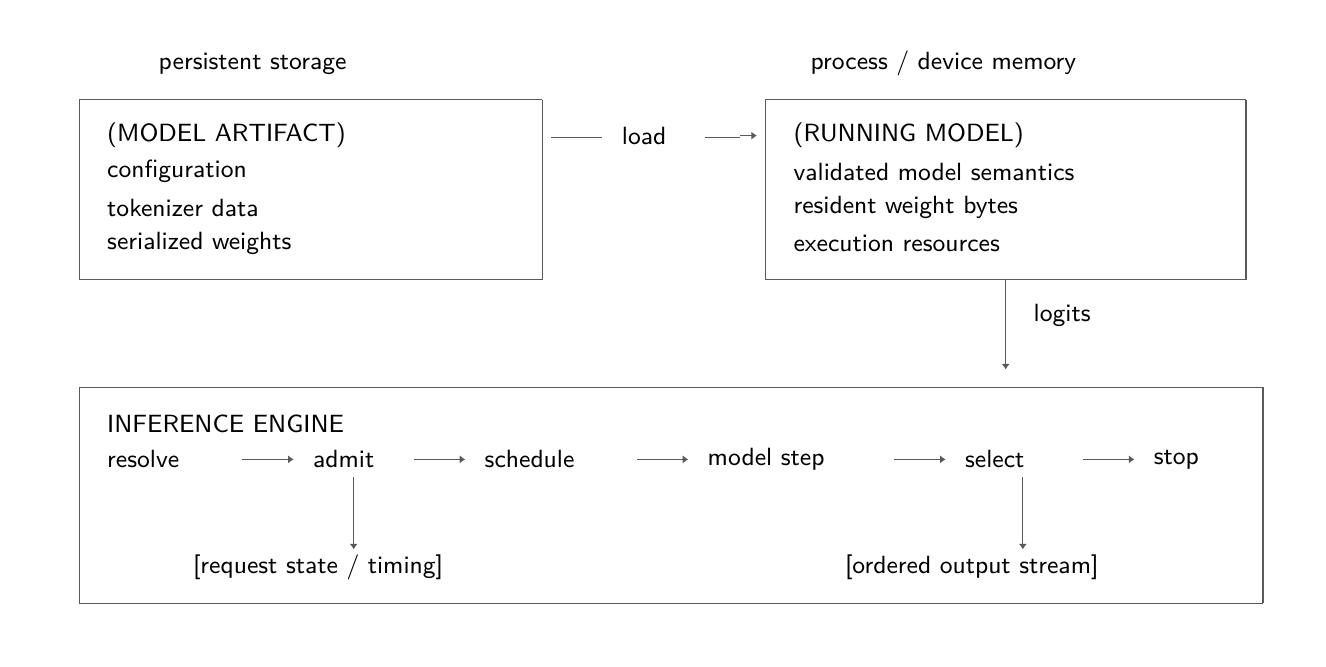
\begin{tikzpicture}[x=6.2pt,y=-13pt,draw=black!65,line width=.45pt]
\path[use as bounding box] (-1,-1) rectangle (73,16);
\node[anchor=west,inner sep=0pt,font=\sffamily\fontsize{9}{11}\selectfont] at (6.6,0) {\begin{adjustbox}{max width=111.60000000000001pt}persistent storage\end{adjustbox}};
\node[anchor=west,inner sep=0pt,font=\sffamily\fontsize{9}{11}\selectfont] at (44.6,0) {\begin{adjustbox}{max width=142.6pt}process / device memory\end{adjustbox}};
\draw (2,1) -- (2.5,1);
\draw (2,1) -- (2,1.5);
\draw (3,1) -- (2.5,1);
\draw (3,1) -- (3.5,1);
\draw (4,1) -- (3.5,1);
\draw (4,1) -- (4.5,1);
\draw (5,1) -- (4.5,1);
\draw (5,1) -- (5.5,1);
\draw (6,1) -- (5.5,1);
\draw (6,1) -- (6.5,1);
\draw (7,1) -- (6.5,1);
\draw (7,1) -- (7.5,1);
\draw (8,1) -- (7.5,1);
\draw (8,1) -- (8.5,1);
\draw (9,1) -- (8.5,1);
\draw (9,1) -- (9.5,1);
\draw (10,1) -- (9.5,1);
\draw (10,1) -- (10.5,1);
\draw (11,1) -- (10.5,1);
\draw (11,1) -- (11.5,1);
\draw (12,1) -- (11.5,1);
\draw (12,1) -- (12.5,1);
\draw (13,1) -- (12.5,1);
\draw (13,1) -- (13.5,1);
\draw (14,1) -- (13.5,1);
\draw (14,1) -- (14.5,1);
\draw (15,1) -- (14.5,1);
\draw (15,1) -- (15.5,1);
\draw (16,1) -- (15.5,1);
\draw (16,1) -- (16.5,1);
\draw (17,1) -- (16.5,1);
\draw (17,1) -- (17.5,1);
\draw (18,1) -- (17.5,1);
\draw (18,1) -- (18.5,1);
\draw (19,1) -- (18.5,1);
\draw (19,1) -- (19.5,1);
\draw (20,1) -- (19.5,1);
\draw (20,1) -- (20.5,1);
\draw (21,1) -- (20.5,1);
\draw (21,1) -- (21.5,1);
\draw (22,1) -- (21.5,1);
\draw (22,1) -- (22.5,1);
\draw (23,1) -- (22.5,1);
\draw (23,1) -- (23.5,1);
\draw (24,1) -- (23.5,1);
\draw (24,1) -- (24.5,1);
\draw (25,1) -- (24.5,1);
\draw (25,1) -- (25.5,1);
\draw (26,1) -- (25.5,1);
\draw (26,1) -- (26.5,1);
\draw (27,1) -- (26.5,1);
\draw (27,1) -- (27.5,1);
\draw (28,1) -- (27.5,1);
\draw (28,1) -- (28.5,1);
\draw (29,1) -- (28.5,1);
\draw (29,1) -- (29,1.5);
\draw (42,1) -- (42.5,1);
\draw (42,1) -- (42,1.5);
\draw (43,1) -- (42.5,1);
\draw (43,1) -- (43.5,1);
\draw (44,1) -- (43.5,1);
\draw (44,1) -- (44.5,1);
\draw (45,1) -- (44.5,1);
\draw (45,1) -- (45.5,1);
\draw (46,1) -- (45.5,1);
\draw (46,1) -- (46.5,1);
\draw (47,1) -- (46.5,1);
\draw (47,1) -- (47.5,1);
\draw (48,1) -- (47.5,1);
\draw (48,1) -- (48.5,1);
\draw (49,1) -- (48.5,1);
\draw (49,1) -- (49.5,1);
\draw (50,1) -- (49.5,1);
\draw (50,1) -- (50.5,1);
\draw (51,1) -- (50.5,1);
\draw (51,1) -- (51.5,1);
\draw (52,1) -- (51.5,1);
\draw (52,1) -- (52.5,1);
\draw (53,1) -- (52.5,1);
\draw (53,1) -- (53.5,1);
\draw (54,1) -- (53.5,1);
\draw (54,1) -- (54.5,1);
\draw (55,1) -- (54.5,1);
\draw (55,1) -- (55.5,1);
\draw (56,1) -- (55.5,1);
\draw (56,1) -- (56.5,1);
\draw (57,1) -- (56.5,1);
\draw (57,1) -- (57.5,1);
\draw (58,1) -- (57.5,1);
\draw (58,1) -- (58.5,1);
\draw (59,1) -- (58.5,1);
\draw (59,1) -- (59.5,1);
\draw (60,1) -- (59.5,1);
\draw (60,1) -- (60.5,1);
\draw (61,1) -- (60.5,1);
\draw (61,1) -- (61.5,1);
\draw (62,1) -- (61.5,1);
\draw (62,1) -- (62.5,1);
\draw (63,1) -- (62.5,1);
\draw (63,1) -- (63.5,1);
\draw (64,1) -- (63.5,1);
\draw (64,1) -- (64.5,1);
\draw (65,1) -- (64.5,1);
\draw (65,1) -- (65.5,1);
\draw (66,1) -- (65.5,1);
\draw (66,1) -- (66.5,1);
\draw (67,1) -- (66.5,1);
\draw (67,1) -- (67.5,1);
\draw (68,1) -- (67.5,1);
\draw (68,1) -- (68.5,1);
\draw (69,1) -- (68.5,1);
\draw (69,1) -- (69.5,1);
\draw (70,1) -- (69.5,1);
\draw (70,1) -- (70,1.5);
\draw (2,2) -- (2,1.5);
\draw (2,2) -- (2,2.5);
\draw (29,2) -- (29,1.5);
\draw (29,2) -- (29,2.5);
\draw[double,double distance=.9pt,line width=.3pt] (30,2) -- (29.5,2);
\draw[double,double distance=.9pt,line width=.3pt] (30,2) -- (30.5,2);
\draw[double,double distance=.9pt,line width=.3pt] (31,2) -- (30.5,2);
\draw[double,double distance=.9pt,line width=.3pt] (31,2) -- (31.5,2);
\draw[double,double distance=.9pt,line width=.3pt] (32,2) -- (31.5,2);
\draw[double,double distance=.9pt,line width=.3pt] (32,2) -- (32.5,2);
\draw[double,double distance=.9pt,line width=.3pt] (39,2) -- (38.5,2);
\draw[double,double distance=.9pt,line width=.3pt] (39,2) -- (39.5,2);
\draw[double,double distance=.9pt,line width=.3pt] (40,2) -- (39.5,2);
\draw[double,double distance=.9pt,line width=.3pt] (40,2) -- (40.5,2);
\draw[-{Latex[length=2pt,width=3pt]}] (40.5,2) -- (41.5,2);
\draw (42,2) -- (42,1.5);
\draw (42,2) -- (42,2.5);
\draw (70,2) -- (70,1.5);
\draw (70,2) -- (70,2.5);
\node[anchor=west,inner sep=0pt,font=\sffamily\fontsize{9}{11}\selectfont] at (3.6,2) {\begin{adjustbox}{max width=99.2pt}(MODEL ARTIFACT)\end{adjustbox}};
\node[anchor=west,inner sep=0pt,font=\sffamily\fontsize{9}{11}\selectfont] at (33.6,2) {\begin{adjustbox}{max width=24.8pt}load\end{adjustbox}};
\node[anchor=west,inner sep=0pt,font=\sffamily\fontsize{9}{11}\selectfont] at (43.6,2) {\begin{adjustbox}{max width=93.0pt}(RUNNING MODEL)\end{adjustbox}};
\draw (2,3) -- (2,2.5);
\draw (2,3) -- (2,3.5);
\draw (29,3) -- (29,2.5);
\draw (29,3) -- (29,3.5);
\draw (42,3) -- (42,2.5);
\draw (42,3) -- (42,3.5);
\draw (70,3) -- (70,2.5);
\draw (70,3) -- (70,3.5);
\node[anchor=west,inner sep=0pt,font=\sffamily\fontsize{9}{11}\selectfont] at (3.6,3) {\begin{adjustbox}{max width=80.60000000000001pt}configuration\end{adjustbox}};
\node[anchor=west,inner sep=0pt,font=\sffamily\fontsize{9}{11}\selectfont] at (43.6,3) {\begin{adjustbox}{max width=155.0pt}validated model semantics\end{adjustbox}};
\draw (2,4) -- (2,3.5);
\draw (2,4) -- (2,4.5);
\draw (29,4) -- (29,3.5);
\draw (29,4) -- (29,4.5);
\draw (42,4) -- (42,3.5);
\draw (42,4) -- (42,4.5);
\draw (70,4) -- (70,3.5);
\draw (70,4) -- (70,4.5);
\node[anchor=west,inner sep=0pt,font=\sffamily\fontsize{9}{11}\selectfont] at (3.6,4) {\begin{adjustbox}{max width=86.8pt}tokenizer data\end{adjustbox}};
\node[anchor=west,inner sep=0pt,font=\sffamily\fontsize{9}{11}\selectfont] at (43.6,4) {\begin{adjustbox}{max width=130.20000000000002pt}resident weight bytes\end{adjustbox}};
\draw (2,5) -- (2,4.5);
\draw (2,5) -- (2,5.5);
\draw (29,5) -- (29,4.5);
\draw (29,5) -- (29,5.5);
\draw (42,5) -- (42,4.5);
\draw (42,5) -- (42,5.5);
\draw (70,5) -- (70,4.5);
\draw (70,5) -- (70,5.5);
\node[anchor=west,inner sep=0pt,font=\sffamily\fontsize{9}{11}\selectfont] at (3.6,5) {\begin{adjustbox}{max width=111.60000000000001pt}serialized weights\end{adjustbox}};
\node[anchor=west,inner sep=0pt,font=\sffamily\fontsize{9}{11}\selectfont] at (43.6,5) {\begin{adjustbox}{max width=117.8pt}execution resources\end{adjustbox}};
\draw (2,6) -- (2.5,6);
\draw (2,6) -- (2,5.5);
\draw (3,6) -- (2.5,6);
\draw (3,6) -- (3.5,6);
\draw (4,6) -- (3.5,6);
\draw (4,6) -- (4.5,6);
\draw (5,6) -- (4.5,6);
\draw (5,6) -- (5.5,6);
\draw (6,6) -- (5.5,6);
\draw (6,6) -- (6.5,6);
\draw (7,6) -- (6.5,6);
\draw (7,6) -- (7.5,6);
\draw (8,6) -- (7.5,6);
\draw (8,6) -- (8.5,6);
\draw (9,6) -- (8.5,6);
\draw (9,6) -- (9.5,6);
\draw (10,6) -- (9.5,6);
\draw (10,6) -- (10.5,6);
\draw (11,6) -- (10.5,6);
\draw (11,6) -- (11.5,6);
\draw (12,6) -- (11.5,6);
\draw (12,6) -- (12.5,6);
\draw (13,6) -- (12.5,6);
\draw (13,6) -- (13.5,6);
\draw (14,6) -- (13.5,6);
\draw (14,6) -- (14.5,6);
\draw (15,6) -- (14.5,6);
\draw (15,6) -- (15.5,6);
\draw (16,6) -- (15.5,6);
\draw (16,6) -- (16.5,6);
\draw (17,6) -- (16.5,6);
\draw (17,6) -- (17.5,6);
\draw (18,6) -- (17.5,6);
\draw (18,6) -- (18.5,6);
\draw (19,6) -- (18.5,6);
\draw (19,6) -- (19.5,6);
\draw (20,6) -- (19.5,6);
\draw (20,6) -- (20.5,6);
\draw (21,6) -- (20.5,6);
\draw (21,6) -- (21.5,6);
\draw (22,6) -- (21.5,6);
\draw (22,6) -- (22.5,6);
\draw (23,6) -- (22.5,6);
\draw (23,6) -- (23.5,6);
\draw (24,6) -- (23.5,6);
\draw (24,6) -- (24.5,6);
\draw (25,6) -- (24.5,6);
\draw (25,6) -- (25.5,6);
\draw (26,6) -- (25.5,6);
\draw (26,6) -- (26.5,6);
\draw (27,6) -- (26.5,6);
\draw (27,6) -- (27.5,6);
\draw (28,6) -- (27.5,6);
\draw (28,6) -- (28.5,6);
\draw (29,6) -- (28.5,6);
\draw (29,6) -- (29,5.5);
\draw (42,6) -- (42.5,6);
\draw (42,6) -- (42,5.5);
\draw (43,6) -- (42.5,6);
\draw (43,6) -- (43.5,6);
\draw (44,6) -- (43.5,6);
\draw (44,6) -- (44.5,6);
\draw (45,6) -- (44.5,6);
\draw (45,6) -- (45.5,6);
\draw (46,6) -- (45.5,6);
\draw (46,6) -- (46.5,6);
\draw (47,6) -- (46.5,6);
\draw (47,6) -- (47.5,6);
\draw (48,6) -- (47.5,6);
\draw (48,6) -- (48.5,6);
\draw (49,6) -- (48.5,6);
\draw (49,6) -- (49.5,6);
\draw (50,6) -- (49.5,6);
\draw (50,6) -- (50.5,6);
\draw (51,6) -- (50.5,6);
\draw (51,6) -- (51.5,6);
\draw (52,6) -- (51.5,6);
\draw (52,6) -- (52.5,6);
\draw (53,6) -- (52.5,6);
\draw (53,6) -- (53.5,6);
\draw (54,6) -- (53.5,6);
\draw (54,6) -- (54.5,6);
\draw (55,6) -- (54.5,6);
\draw (55,6) -- (55.5,6);
\draw (56,6) -- (55.5,6);
\draw (56,6) -- (56.5,6);
\draw (56,6) -- (56,6.5);
\draw (57,6) -- (56.5,6);
\draw (57,6) -- (57.5,6);
\draw (58,6) -- (57.5,6);
\draw (58,6) -- (58.5,6);
\draw (59,6) -- (58.5,6);
\draw (59,6) -- (59.5,6);
\draw (60,6) -- (59.5,6);
\draw (60,6) -- (60.5,6);
\draw (61,6) -- (60.5,6);
\draw (61,6) -- (61.5,6);
\draw (62,6) -- (61.5,6);
\draw (62,6) -- (62.5,6);
\draw (63,6) -- (62.5,6);
\draw (63,6) -- (63.5,6);
\draw (64,6) -- (63.5,6);
\draw (64,6) -- (64.5,6);
\draw (65,6) -- (64.5,6);
\draw (65,6) -- (65.5,6);
\draw (66,6) -- (65.5,6);
\draw (66,6) -- (66.5,6);
\draw (67,6) -- (66.5,6);
\draw (67,6) -- (67.5,6);
\draw (68,6) -- (67.5,6);
\draw (68,6) -- (68.5,6);
\draw (69,6) -- (68.5,6);
\draw (69,6) -- (69.5,6);
\draw (70,6) -- (69.5,6);
\draw (70,6) -- (70,5.5);
\draw (56,7) -- (56,6.5);
\draw (56,7) -- (56,7.5);
\node[anchor=west,inner sep=0pt,font=\sffamily\fontsize{9}{11}\selectfont] at (57.6,7) {\begin{adjustbox}{max width=37.2pt}logits\end{adjustbox}};
\draw[-{Latex[length=2pt,width=3pt]}] (56,7.5) -- (56,8.5);
\draw (2,9) -- (2.5,9);
\draw (2,9) -- (2,9.5);
\draw (3,9) -- (2.5,9);
\draw (3,9) -- (3.5,9);
\draw (4,9) -- (3.5,9);
\draw (4,9) -- (4.5,9);
\draw (5,9) -- (4.5,9);
\draw (5,9) -- (5.5,9);
\draw (6,9) -- (5.5,9);
\draw (6,9) -- (6.5,9);
\draw (7,9) -- (6.5,9);
\draw (7,9) -- (7.5,9);
\draw (8,9) -- (7.5,9);
\draw (8,9) -- (8.5,9);
\draw (9,9) -- (8.5,9);
\draw (9,9) -- (9.5,9);
\draw (10,9) -- (9.5,9);
\draw (10,9) -- (10.5,9);
\draw (11,9) -- (10.5,9);
\draw (11,9) -- (11.5,9);
\draw (12,9) -- (11.5,9);
\draw (12,9) -- (12.5,9);
\draw (13,9) -- (12.5,9);
\draw (13,9) -- (13.5,9);
\draw (14,9) -- (13.5,9);
\draw (14,9) -- (14.5,9);
\draw (15,9) -- (14.5,9);
\draw (15,9) -- (15.5,9);
\draw (16,9) -- (15.5,9);
\draw (16,9) -- (16.5,9);
\draw (17,9) -- (16.5,9);
\draw (17,9) -- (17.5,9);
\draw (18,9) -- (17.5,9);
\draw (18,9) -- (18.5,9);
\draw (19,9) -- (18.5,9);
\draw (19,9) -- (19.5,9);
\draw (20,9) -- (19.5,9);
\draw (20,9) -- (20.5,9);
\draw (21,9) -- (20.5,9);
\draw (21,9) -- (21.5,9);
\draw (22,9) -- (21.5,9);
\draw (22,9) -- (22.5,9);
\draw (23,9) -- (22.5,9);
\draw (23,9) -- (23.5,9);
\draw (24,9) -- (23.5,9);
\draw (24,9) -- (24.5,9);
\draw (25,9) -- (24.5,9);
\draw (25,9) -- (25.5,9);
\draw (26,9) -- (25.5,9);
\draw (26,9) -- (26.5,9);
\draw (27,9) -- (26.5,9);
\draw (27,9) -- (27.5,9);
\draw (28,9) -- (27.5,9);
\draw (28,9) -- (28.5,9);
\draw (29,9) -- (28.5,9);
\draw (29,9) -- (29.5,9);
\draw (30,9) -- (29.5,9);
\draw (30,9) -- (30.5,9);
\draw (31,9) -- (30.5,9);
\draw (31,9) -- (31.5,9);
\draw (32,9) -- (31.5,9);
\draw (32,9) -- (32.5,9);
\draw (33,9) -- (32.5,9);
\draw (33,9) -- (33.5,9);
\draw (34,9) -- (33.5,9);
\draw (34,9) -- (34.5,9);
\draw (35,9) -- (34.5,9);
\draw (35,9) -- (35.5,9);
\draw (36,9) -- (35.5,9);
\draw (36,9) -- (36.5,9);
\draw (37,9) -- (36.5,9);
\draw (37,9) -- (37.5,9);
\draw (38,9) -- (37.5,9);
\draw (38,9) -- (38.5,9);
\draw (39,9) -- (38.5,9);
\draw (39,9) -- (39.5,9);
\draw (40,9) -- (39.5,9);
\draw (40,9) -- (40.5,9);
\draw (41,9) -- (40.5,9);
\draw (41,9) -- (41.5,9);
\draw (42,9) -- (41.5,9);
\draw (42,9) -- (42.5,9);
\draw (43,9) -- (42.5,9);
\draw (43,9) -- (43.5,9);
\draw (44,9) -- (43.5,9);
\draw (44,9) -- (44.5,9);
\draw (45,9) -- (44.5,9);
\draw (45,9) -- (45.5,9);
\draw (46,9) -- (45.5,9);
\draw (46,9) -- (46.5,9);
\draw (47,9) -- (46.5,9);
\draw (47,9) -- (47.5,9);
\draw (48,9) -- (47.5,9);
\draw (48,9) -- (48.5,9);
\draw (49,9) -- (48.5,9);
\draw (49,9) -- (49.5,9);
\draw (50,9) -- (49.5,9);
\draw (50,9) -- (50.5,9);
\draw (51,9) -- (50.5,9);
\draw (51,9) -- (51.5,9);
\draw (52,9) -- (51.5,9);
\draw (52,9) -- (52.5,9);
\draw (53,9) -- (52.5,9);
\draw (53,9) -- (53.5,9);
\draw (54,9) -- (53.5,9);
\draw (54,9) -- (54.5,9);
\draw (55,9) -- (54.5,9);
\draw (55,9) -- (55.5,9);
\draw (56,9) -- (55.5,9);
\draw (56,9) -- (56.5,9);
\draw (57,9) -- (56.5,9);
\draw (57,9) -- (57.5,9);
\draw (58,9) -- (57.5,9);
\draw (58,9) -- (58.5,9);
\draw (59,9) -- (58.5,9);
\draw (59,9) -- (59.5,9);
\draw (60,9) -- (59.5,9);
\draw (60,9) -- (60.5,9);
\draw (61,9) -- (60.5,9);
\draw (61,9) -- (61.5,9);
\draw (62,9) -- (61.5,9);
\draw (62,9) -- (62.5,9);
\draw (63,9) -- (62.5,9);
\draw (63,9) -- (63.5,9);
\draw (64,9) -- (63.5,9);
\draw (64,9) -- (64.5,9);
\draw (65,9) -- (64.5,9);
\draw (65,9) -- (65.5,9);
\draw (66,9) -- (65.5,9);
\draw (66,9) -- (66.5,9);
\draw (67,9) -- (66.5,9);
\draw (67,9) -- (67.5,9);
\draw (68,9) -- (67.5,9);
\draw (68,9) -- (68.5,9);
\draw (69,9) -- (68.5,9);
\draw (69,9) -- (69.5,9);
\draw (70,9) -- (69.5,9);
\draw (70,9) -- (70.5,9);
\draw (71,9) -- (70.5,9);
\draw (71,9) -- (71,9.5);
\draw (2,10) -- (2,9.5);
\draw (2,10) -- (2,10.5);
\draw (71,10) -- (71,9.5);
\draw (71,10) -- (71,10.5);
\node[anchor=west,inner sep=0pt,font=\sffamily\fontsize{9}{11}\selectfont] at (3.6,10) {\begin{adjustbox}{max width=99.2pt}INFERENCE ENGINE\end{adjustbox}};
\draw (2,11) -- (2,10.5);
\draw (2,11) -- (2,11.5);
\draw (12,11) -- (11.5,11);
\draw (12,11) -- (12.5,11);
\draw (13,11) -- (12.5,11);
\draw (13,11) -- (13.5,11);
\draw[-{Latex[length=2pt,width=3pt]}] (13.5,11) -- (14.5,11);
\draw (22,11) -- (21.5,11);
\draw (22,11) -- (22.5,11);
\draw (23,11) -- (22.5,11);
\draw (23,11) -- (23.5,11);
\draw[-{Latex[length=2pt,width=3pt]}] (23.5,11) -- (24.5,11);
\draw (35,11) -- (34.5,11);
\draw (35,11) -- (35.5,11);
\draw (36,11) -- (35.5,11);
\draw (36,11) -- (36.5,11);
\draw[-{Latex[length=2pt,width=3pt]}] (36.5,11) -- (37.5,11);
\draw (50,11) -- (49.5,11);
\draw (50,11) -- (50.5,11);
\draw (51,11) -- (50.5,11);
\draw (51,11) -- (51.5,11);
\draw[-{Latex[length=2pt,width=3pt]}] (51.5,11) -- (52.5,11);
\draw (61,11) -- (60.5,11);
\draw (61,11) -- (61.5,11);
\draw (62,11) -- (61.5,11);
\draw (62,11) -- (62.5,11);
\draw[-{Latex[length=2pt,width=3pt]}] (62.5,11) -- (63.5,11);
\draw (71,11) -- (71,10.5);
\draw (71,11) -- (71,11.5);
\node[anchor=west,inner sep=0pt,font=\sffamily\fontsize{9}{11}\selectfont] at (3.6,11) {\begin{adjustbox}{max width=43.4pt}resolve\end{adjustbox}};
\node[anchor=west,inner sep=0pt,font=\sffamily\fontsize{9}{11}\selectfont] at (15.6,11) {\begin{adjustbox}{max width=31.0pt}admit\end{adjustbox}};
\node[anchor=west,inner sep=0pt,font=\sffamily\fontsize{9}{11}\selectfont] at (25.6,11) {\begin{adjustbox}{max width=49.6pt}schedule\end{adjustbox}};
\node[anchor=west,inner sep=0pt,font=\sffamily\fontsize{9}{11}\selectfont] at (38.6,11) {\begin{adjustbox}{max width=62.0pt}model step\end{adjustbox}};
\node[anchor=west,inner sep=0pt,font=\sffamily\fontsize{9}{11}\selectfont] at (53.6,11) {\begin{adjustbox}{max width=37.2pt}select\end{adjustbox}};
\node[anchor=west,inner sep=0pt,font=\sffamily\fontsize{9}{11}\selectfont] at (64.6,11) {\begin{adjustbox}{max width=24.8pt}stop\end{adjustbox}};
\draw (2,12) -- (2,11.5);
\draw (2,12) -- (2,12.5);
\draw (18,12) -- (18,11.5);
\draw (18,12) -- (18,12.5);
\draw (57,12) -- (57,11.5);
\draw (57,12) -- (57,12.5);
\draw (71,12) -- (71,11.5);
\draw (71,12) -- (71,12.5);
\draw (2,13) -- (2,12.5);
\draw (2,13) -- (2,13.5);
\draw[-{Latex[length=2pt,width=3pt]}] (18,12.5) -- (18,13.5);
\draw[-{Latex[length=2pt,width=3pt]}] (57,12.5) -- (57,13.5);
\draw (71,13) -- (71,12.5);
\draw (71,13) -- (71,13.5);
\draw (2,14) -- (2,13.5);
\draw (2,14) -- (2,14.5);
\draw (71,14) -- (71,13.5);
\draw (71,14) -- (71,14.5);
\node[anchor=west,inner sep=0pt,font=\sffamily\fontsize{9}{11}\selectfont] at (8.6,14) {\begin{adjustbox}{max width=148.8pt}[request state / timing]\end{adjustbox}};
\node[anchor=west,inner sep=0pt,font=\sffamily\fontsize{9}{11}\selectfont] at (46.6,14) {\begin{adjustbox}{max width=142.6pt}[ordered output stream]\end{adjustbox}};
\draw (2,15) -- (2.5,15);
\draw (2,15) -- (2,14.5);
\draw (3,15) -- (2.5,15);
\draw (3,15) -- (3.5,15);
\draw (4,15) -- (3.5,15);
\draw (4,15) -- (4.5,15);
\draw (5,15) -- (4.5,15);
\draw (5,15) -- (5.5,15);
\draw (6,15) -- (5.5,15);
\draw (6,15) -- (6.5,15);
\draw (7,15) -- (6.5,15);
\draw (7,15) -- (7.5,15);
\draw (8,15) -- (7.5,15);
\draw (8,15) -- (8.5,15);
\draw (9,15) -- (8.5,15);
\draw (9,15) -- (9.5,15);
\draw (10,15) -- (9.5,15);
\draw (10,15) -- (10.5,15);
\draw (11,15) -- (10.5,15);
\draw (11,15) -- (11.5,15);
\draw (12,15) -- (11.5,15);
\draw (12,15) -- (12.5,15);
\draw (13,15) -- (12.5,15);
\draw (13,15) -- (13.5,15);
\draw (14,15) -- (13.5,15);
\draw (14,15) -- (14.5,15);
\draw (15,15) -- (14.5,15);
\draw (15,15) -- (15.5,15);
\draw (16,15) -- (15.5,15);
\draw (16,15) -- (16.5,15);
\draw (17,15) -- (16.5,15);
\draw (17,15) -- (17.5,15);
\draw (18,15) -- (17.5,15);
\draw (18,15) -- (18.5,15);
\draw (19,15) -- (18.5,15);
\draw (19,15) -- (19.5,15);
\draw (20,15) -- (19.5,15);
\draw (20,15) -- (20.5,15);
\draw (21,15) -- (20.5,15);
\draw (21,15) -- (21.5,15);
\draw (22,15) -- (21.5,15);
\draw (22,15) -- (22.5,15);
\draw (23,15) -- (22.5,15);
\draw (23,15) -- (23.5,15);
\draw (24,15) -- (23.5,15);
\draw (24,15) -- (24.5,15);
\draw (25,15) -- (24.5,15);
\draw (25,15) -- (25.5,15);
\draw (26,15) -- (25.5,15);
\draw (26,15) -- (26.5,15);
\draw (27,15) -- (26.5,15);
\draw (27,15) -- (27.5,15);
\draw (28,15) -- (27.5,15);
\draw (28,15) -- (28.5,15);
\draw (29,15) -- (28.5,15);
\draw (29,15) -- (29.5,15);
\draw (30,15) -- (29.5,15);
\draw (30,15) -- (30.5,15);
\draw (31,15) -- (30.5,15);
\draw (31,15) -- (31.5,15);
\draw (32,15) -- (31.5,15);
\draw (32,15) -- (32.5,15);
\draw (33,15) -- (32.5,15);
\draw (33,15) -- (33.5,15);
\draw (34,15) -- (33.5,15);
\draw (34,15) -- (34.5,15);
\draw (35,15) -- (34.5,15);
\draw (35,15) -- (35.5,15);
\draw (36,15) -- (35.5,15);
\draw (36,15) -- (36.5,15);
\draw (37,15) -- (36.5,15);
\draw (37,15) -- (37.5,15);
\draw (38,15) -- (37.5,15);
\draw (38,15) -- (38.5,15);
\draw (39,15) -- (38.5,15);
\draw (39,15) -- (39.5,15);
\draw (40,15) -- (39.5,15);
\draw (40,15) -- (40.5,15);
\draw (41,15) -- (40.5,15);
\draw (41,15) -- (41.5,15);
\draw (42,15) -- (41.5,15);
\draw (42,15) -- (42.5,15);
\draw (43,15) -- (42.5,15);
\draw (43,15) -- (43.5,15);
\draw (44,15) -- (43.5,15);
\draw (44,15) -- (44.5,15);
\draw (45,15) -- (44.5,15);
\draw (45,15) -- (45.5,15);
\draw (46,15) -- (45.5,15);
\draw (46,15) -- (46.5,15);
\draw (47,15) -- (46.5,15);
\draw (47,15) -- (47.5,15);
\draw (48,15) -- (47.5,15);
\draw (48,15) -- (48.5,15);
\draw (49,15) -- (48.5,15);
\draw (49,15) -- (49.5,15);
\draw (50,15) -- (49.5,15);
\draw (50,15) -- (50.5,15);
\draw (51,15) -- (50.5,15);
\draw (51,15) -- (51.5,15);
\draw (52,15) -- (51.5,15);
\draw (52,15) -- (52.5,15);
\draw (53,15) -- (52.5,15);
\draw (53,15) -- (53.5,15);
\draw (54,15) -- (53.5,15);
\draw (54,15) -- (54.5,15);
\draw (55,15) -- (54.5,15);
\draw (55,15) -- (55.5,15);
\draw (56,15) -- (55.5,15);
\draw (56,15) -- (56.5,15);
\draw (57,15) -- (56.5,15);
\draw (57,15) -- (57.5,15);
\draw (58,15) -- (57.5,15);
\draw (58,15) -- (58.5,15);
\draw (59,15) -- (58.5,15);
\draw (59,15) -- (59.5,15);
\draw (60,15) -- (59.5,15);
\draw (60,15) -- (60.5,15);
\draw (61,15) -- (60.5,15);
\draw (61,15) -- (61.5,15);
\draw (62,15) -- (61.5,15);
\draw (62,15) -- (62.5,15);
\draw (63,15) -- (62.5,15);
\draw (63,15) -- (63.5,15);
\draw (64,15) -- (63.5,15);
\draw (64,15) -- (64.5,15);
\draw (65,15) -- (64.5,15);
\draw (65,15) -- (65.5,15);
\draw (66,15) -- (65.5,15);
\draw (66,15) -- (66.5,15);
\draw (67,15) -- (66.5,15);
\draw (67,15) -- (67.5,15);
\draw (68,15) -- (67.5,15);
\draw (68,15) -- (68.5,15);
\draw (69,15) -- (68.5,15);
\draw (69,15) -- (69.5,15);
\draw (70,15) -- (69.5,15);
\draw (70,15) -- (70.5,15);
\draw (71,15) -- (70.5,15);
\draw (71,15) -- (71,14.5);
\end{tikzpicture}
\end{adjustbox}\end{center}

Parentheses denote data treated as immutable during a request. Brackets
denote mutable state with an owner. The distinction is logical: an
implementation may map weights from disk, copy them to RAM, mirror them
on a device, or keep more than one packed representation. Whatever the
placement, request code must know which bytes are shared, which bytes
may be mutated, and who releases each resource.

\begin{quote}
\textbf{FIRST PRINCIPLE} A model defines a computation. An inference
engine owns the process of using that computation to advance requests to
observable terminal outcomes.
\end{quote}

This definition is intentionally about responsibility, not process
topology. An engine can live inside a command-line program, a Python
process, a mobile app, or a fleet of services. Moving a boundary across
processes changes communication and failure costs; it does not remove
the responsibility.

\subsection{Training and inference solve different
problems}\label{training-and-inference-solve-different-problems}

Training changes model parameters. Given examples, an objective, and an
optimization procedure, training repeatedly computes predictions and
gradients and updates weights. Its central state includes parameters,
gradients, optimizer statistics, training examples, and checkpoints. A
training system cares deeply about distributed gradient communication,
update correctness, checkpoint recovery, and sample throughput.

Inference uses already-chosen parameters to answer requests. In the
ordinary case, it must not update the model weights. Its central state
is instead the state needed to evaluate inputs and continue sequences:
loaded weights, temporary activations, per-request history, cached
intermediate state, selection state, queues, and streams. An inference
service also has to handle arrival bursts, deadlines, cancellation,
failures, resource limits, and protocol behavior.

The same mathematical model may appear in both systems, and both perform
forward computation, but their ownership and economics differ:

{\def\LTcaptype{none} % do not increment counter
\begin{longtable}[]{@{}
  >{\raggedright\arraybackslash}p{(\linewidth - 4\tabcolsep) * \real{0.3333}}
  >{\raggedright\arraybackslash}p{(\linewidth - 4\tabcolsep) * \real{0.3333}}
  >{\raggedright\arraybackslash}p{(\linewidth - 4\tabcolsep) * \real{0.3333}}@{}}
\toprule\noalign{}
\begin{minipage}[b]{\linewidth}\raggedright
Concern
\end{minipage} & \begin{minipage}[b]{\linewidth}\raggedright
Training
\end{minipage} & \begin{minipage}[b]{\linewidth}\raggedright
Inference
\end{minipage} \\
\midrule\noalign{}
\endhead
\bottomrule\noalign{}
\endlastfoot
Weight state & Deliberately updated & Normally immutable during a
request \\
Primary unit & Optimization step / sample batch & Request / sequence /
emitted token \\
Repeated state & Gradients and optimizer state & Generation history and
reusable inference state \\
Scheduling goal & Efficient, correct parameter updates & Latency,
throughput, fairness, and bounded memory \\
External contract & Checkpoint and training progress & Ordered output
and terminal request behavior \\
Common failure question & Can the update recover? & Which requests fail,
and is their state released? \\
\end{longtable}
}

This book is about inference. Later we may use an engine during
evaluation or post-training workflows, but we will keep the runtime
contract visible. Calling the same model function does not make the
surrounding system the same.

\subsection{Four layers that are often collapsed into ``the
model''}\label{four-layers-that-are-often-collapsed-into-the-model}

The word \emph{model} is overloaded in ordinary conversation. A precise
system map needs at least four layers.

\subsubsection{The mathematical model}\label{the-mathematical-model}

The mathematical model maps inputs and state to outputs. For a causal
language model, a useful future view is that a token history leads to a
score for every possible next token. We will derive that computation
later. In Chapter 1, its contract is only ``produce candidates for the
next token.''

\subsubsection{Model representation and
execution}\label{model-representation-and-execution}

The representation layer interprets artifacts: tensor names, shapes,
dtypes, layouts, tokenizer configuration, and architecture metadata.
Execution implementations perform operations on some substrate. That may
be scalar CPU code, vectorized CPU code, Metal, CUDA, or another
backend. A compiled backend is not proof that it supports this model,
this shape, or this request.

\subsubsection{The inference runtime or
engine}\label{the-inference-runtime-or-engine}

The runtime owns live request progress and resource coordination. It
resolves a running model, admits work, decides when it may execute,
invokes model steps, applies selection and stopping policy, emits
ordered events, accounts for work, and releases state. Some projects use
\emph{runtime} for a narrower execution layer and \emph{engine} for the
full coordinator. We will qualify external names, but our book uses
\textbf{inference engine} for the combined request-to-outcome
responsibility.

\subsubsection{The serving and operational
surface}\label{the-serving-and-operational-surface}

A server accepts requests through a protocol and converts them to the
engine's internal form. It may parse HTTP, authenticate, validate
schemas, format Server-Sent Events, enforce body limits, and map
internal terminal causes to wire finish reasons. A service adds
deployment concerns: replicas, load balancing, quotas, health, rollout,
rollback, observability, and service-level objectives.

The
\href{https://github.com/hermonai/inside-the-llm-engine/blob/astra-visual-rewrite/diagrams/runtime/inference-stack.txt}{canonical
inference-stack diagram} shows the roles:

\begin{verbatim}
application
    |
    v
library API  ---------------- direct/offline generation
    |
    v
inference engine
    +--> provider choice  --> local | remote | managed capability
    +--> hardware backend --> scalar CPU | SIMD CPU | Metal | CUDA | ...
    |
    v
server  - - > protocol validation, HTTP/gRPC/SSE, multi-client boundary
    |
    v
service - - > deployment, replicas, auth, quotas, SLOs, operations
\end{verbatim}

The diagram is not a mandatory call graph. An offline library may embed
the engine without a server. An online system may split API, engine
core, and device workers into separate processes. A managed provider may
hide every layer below an API. The roles remain useful because they
identify contracts and owners.

\subsubsection{Provider is not backend}\label{provider-is-not-backend}

Projects use these words differently, so we need a book convention.

A \textbf{provider} offers or selects an inference capability: for
example, local, remote, or managed execution, possibly associated with
credentials, placement, or a model namespace. A \textbf{backend}
implements model operations on a hardware and runtime substrate. A local
provider might choose a Metal backend on one machine and a CPU backend
on another. A remote provider may hide its backend entirely.

This distinction prevents two common reasoning errors. First, routing a
request to ``local'' does not tell us whether it runs on CPU or GPU.
Second, compiling a CUDA backend does not tell us that a request was
routed to it. We must trace both the provider decision and the backend
selection before making a current execution claim.

\subsection{The engine coordinates compute, memory, and
requests}\label{the-engine-coordinates-compute-memory-and-requests}

An inference engine sits where three systems meet.

\textbf{Compute} asks which operations must run, in what order, with
what shapes, dtypes, and dependencies. A model step eventually produces
candidate scores. Selection policy turns those scores into a token
decision.

\textbf{Memory} asks where artifact bytes, resident weights, temporary
activations, and per-request state live; who may mutate them; whether
they can be shared; and when they can be released. The weight file may
be much larger than one request's state, but mutable request state is
often the harder concurrency problem because a small ownership error can
produce plausible, wrong text.

\textbf{Requests} ask who may enter, when work runs, how progress is
streamed, what cancellation means, which limits stop generation, how
failures are isolated, and when capacity becomes reusable. A
mathematically correct forward pass can still belong to a broken engine
if output is reordered, cancellation leaks state, or two terminals are
reported.

These domains interact. Admitting another request increases memory
demand. Combining work can improve hardware utilization but delay a
particular token. Retaining computed state may reduce future compute
while consuming capacity. Moving work to a device can accelerate a large
operation while adding transfer, launch, and synchronization costs. The
engine is where those tradeoffs become policy rather than slogans.

\subsection{Control plane and data
plane}\label{control-plane-and-data-plane}

We will frequently separate two kinds of work.

The \textbf{control plane} makes decisions and maintains coordination
metadata. It validates and resolves requests, admits them, chooses
models and backends, schedules steps, applies stopping and cancellation,
records metrics, and decides when to release resources.

The \textbf{data plane} moves and transforms the bytes that implement
inference. It loads weight data, reads token and state arrays, runs
tensor operations, produces candidate scores, selects or transfers token
identities, and sends output bytes.

\begin{center}\begin{adjustbox}{max width=\linewidth}% Legacy topology preserved as native vectors and typeset labels.
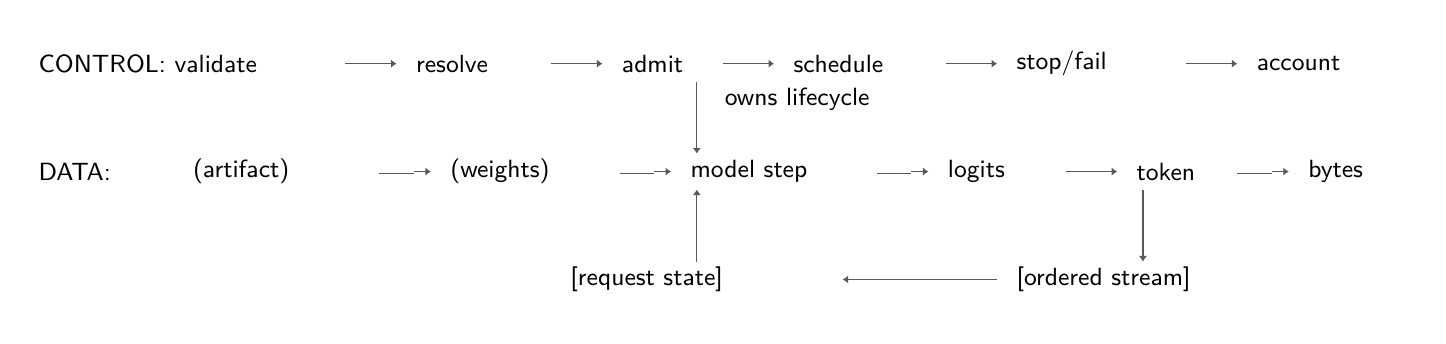
\begin{tikzpicture}[x=6.2pt,y=-13pt,draw=black!65,line width=.45pt]
\path[use as bounding box] (-1,-1) rectangle (80,7);
\draw (18,0) -- (17.5,0);
\draw (18,0) -- (18.5,0);
\draw (19,0) -- (18.5,0);
\draw (19,0) -- (19.5,0);
\draw[-{Latex[length=2pt,width=3pt]}] (19.5,0) -- (20.5,0);
\draw (30,0) -- (29.5,0);
\draw (30,0) -- (30.5,0);
\draw (31,0) -- (30.5,0);
\draw (31,0) -- (31.5,0);
\draw[-{Latex[length=2pt,width=3pt]}] (31.5,0) -- (32.5,0);
\draw (40,0) -- (39.5,0);
\draw (40,0) -- (40.5,0);
\draw (41,0) -- (40.5,0);
\draw (41,0) -- (41.5,0);
\draw[-{Latex[length=2pt,width=3pt]}] (41.5,0) -- (42.5,0);
\draw (53,0) -- (52.5,0);
\draw (53,0) -- (53.5,0);
\draw (54,0) -- (53.5,0);
\draw (54,0) -- (54.5,0);
\draw[-{Latex[length=2pt,width=3pt]}] (54.5,0) -- (55.5,0);
\draw (67,0) -- (66.5,0);
\draw (67,0) -- (67.5,0);
\draw (68,0) -- (67.5,0);
\draw (68,0) -- (68.5,0);
\draw[-{Latex[length=2pt,width=3pt]}] (68.5,0) -- (69.5,0);
\node[anchor=west,inner sep=0pt,font=\sffamily\fontsize{9}{11}\selectfont] at (-0.4,0) {\begin{adjustbox}{max width=105.4pt}CONTROL: validate\end{adjustbox}};
\node[anchor=west,inner sep=0pt,font=\sffamily\fontsize{9}{11}\selectfont] at (21.6,0) {\begin{adjustbox}{max width=43.4pt}resolve\end{adjustbox}};
\node[anchor=west,inner sep=0pt,font=\sffamily\fontsize{9}{11}\selectfont] at (33.6,0) {\begin{adjustbox}{max width=31.0pt}admit\end{adjustbox}};
\node[anchor=west,inner sep=0pt,font=\sffamily\fontsize{9}{11}\selectfont] at (43.6,0) {\begin{adjustbox}{max width=49.6pt}schedule\end{adjustbox}};
\node[anchor=west,inner sep=0pt,font=\sffamily\fontsize{9}{11}\selectfont] at (56.6,0) {\begin{adjustbox}{max width=55.800000000000004pt}stop/fail\end{adjustbox}};
\node[anchor=west,inner sep=0pt,font=\sffamily\fontsize{9}{11}\selectfont] at (70.6,0) {\begin{adjustbox}{max width=43.4pt}account\end{adjustbox}};
\draw (38,1) -- (38,0.5);
\draw (38,1) -- (38,1.5);
\node[anchor=west,inner sep=0pt,font=\sffamily\fontsize{9}{11}\selectfont] at (39.6,1) {\begin{adjustbox}{max width=86.8pt}owns lifecycle\end{adjustbox}};
\draw[-{Latex[length=2pt,width=3pt]}] (38,1.5) -- (38,2.5);
\draw[double,double distance=.9pt,line width=.3pt] (20,3) -- (19.5,3);
\draw[double,double distance=.9pt,line width=.3pt] (20,3) -- (20.5,3);
\draw[double,double distance=.9pt,line width=.3pt] (21,3) -- (20.5,3);
\draw[double,double distance=.9pt,line width=.3pt] (21,3) -- (21.5,3);
\draw[-{Latex[length=2pt,width=3pt]}] (21.5,3) -- (22.5,3);
\draw[double,double distance=.9pt,line width=.3pt] (34,3) -- (33.5,3);
\draw[double,double distance=.9pt,line width=.3pt] (34,3) -- (34.5,3);
\draw[double,double distance=.9pt,line width=.3pt] (35,3) -- (34.5,3);
\draw[double,double distance=.9pt,line width=.3pt] (35,3) -- (35.5,3);
\draw[-{Latex[length=2pt,width=3pt]}] (35.5,3) -- (36.5,3);
\draw[double,double distance=.9pt,line width=.3pt] (49,3) -- (48.5,3);
\draw[double,double distance=.9pt,line width=.3pt] (49,3) -- (49.5,3);
\draw[double,double distance=.9pt,line width=.3pt] (50,3) -- (49.5,3);
\draw[double,double distance=.9pt,line width=.3pt] (50,3) -- (50.5,3);
\draw[-{Latex[length=2pt,width=3pt]}] (50.5,3) -- (51.5,3);
\draw (60,3) -- (59.5,3);
\draw (60,3) -- (60.5,3);
\draw (61,3) -- (60.5,3);
\draw (61,3) -- (61.5,3);
\draw[-{Latex[length=2pt,width=3pt]}] (61.5,3) -- (62.5,3);
\draw[double,double distance=.9pt,line width=.3pt] (70,3) -- (69.5,3);
\draw[double,double distance=.9pt,line width=.3pt] (70,3) -- (70.5,3);
\draw[double,double distance=.9pt,line width=.3pt] (71,3) -- (70.5,3);
\draw[double,double distance=.9pt,line width=.3pt] (71,3) -- (71.5,3);
\draw[-{Latex[length=2pt,width=3pt]}] (71.5,3) -- (72.5,3);
\node[anchor=west,inner sep=0pt,font=\sffamily\fontsize{9}{11}\selectfont] at (-0.4,3) {\begin{adjustbox}{max width=31.0pt}DATA:\end{adjustbox}};
\node[anchor=west,inner sep=0pt,font=\sffamily\fontsize{9}{11}\selectfont] at (8.6,3) {\begin{adjustbox}{max width=62.0pt}(artifact)\end{adjustbox}};
\node[anchor=west,inner sep=0pt,font=\sffamily\fontsize{9}{11}\selectfont] at (23.6,3) {\begin{adjustbox}{max width=55.800000000000004pt}(weights)\end{adjustbox}};
\node[anchor=west,inner sep=0pt,font=\sffamily\fontsize{9}{11}\selectfont] at (37.6,3) {\begin{adjustbox}{max width=62.0pt}model step\end{adjustbox}};
\node[anchor=west,inner sep=0pt,font=\sffamily\fontsize{9}{11}\selectfont] at (52.6,3) {\begin{adjustbox}{max width=37.2pt}logits\end{adjustbox}};
\node[anchor=west,inner sep=0pt,font=\sffamily\fontsize{9}{11}\selectfont] at (63.6,3) {\begin{adjustbox}{max width=31.0pt}token\end{adjustbox}};
\node[anchor=west,inner sep=0pt,font=\sffamily\fontsize{9}{11}\selectfont] at (73.6,3) {\begin{adjustbox}{max width=31.0pt}bytes\end{adjustbox}};
\draw[-{Latex[length=2pt,width=3pt]}] (38,4.5) -- (38,3.5);
\draw (64,4) -- (64,3.5);
\draw (64,4) -- (64,4.5);
\draw (38,5) -- (38,4.5);
\draw (38,5) -- (38,5.5);
\draw[-{Latex[length=2pt,width=3pt]}] (64,4.5) -- (64,5.5);
\draw[-{Latex[length=2pt,width=3pt]}] (47.5,6) -- (46.5,6);
\draw (48,6) -- (47.5,6);
\draw (48,6) -- (48.5,6);
\draw (49,6) -- (48.5,6);
\draw (49,6) -- (49.5,6);
\draw (50,6) -- (49.5,6);
\draw (50,6) -- (50.5,6);
\draw (51,6) -- (50.5,6);
\draw (51,6) -- (51.5,6);
\draw (52,6) -- (51.5,6);
\draw (52,6) -- (52.5,6);
\draw (53,6) -- (52.5,6);
\draw (53,6) -- (53.5,6);
\draw (54,6) -- (53.5,6);
\draw (54,6) -- (54.5,6);
\draw (55,6) -- (54.5,6);
\draw (55,6) -- (55.5,6);
\node[anchor=west,inner sep=0pt,font=\sffamily\fontsize{9}{11}\selectfont] at (30.6,6) {\begin{adjustbox}{max width=93.0pt}[request state]\end{adjustbox}};
\node[anchor=west,inner sep=0pt,font=\sffamily\fontsize{9}{11}\selectfont] at (56.6,6) {\begin{adjustbox}{max width=99.2pt}[ordered stream]\end{adjustbox}};
\end{tikzpicture}
\end{adjustbox}\end{center}

This is a reasoning tool, not a claim that the planes require separate
machines. ENGINE-0 puts both in one synchronous Rust call. vLLM V1, by
contrast, documents an API-server process, an engine-core process, and
worker processes, making some of the split physical as well as
conceptual. The API process performs input processing and streaming; the
engine core schedules and manages KV state; workers perform model
execution on devices
(\href{https://docs.vllm.ai/en/latest/design/arch_overview/}{vLLM
architecture overview}). The canonical
\href{https://github.com/hermonai/inside-the-llm-engine/blob/astra-visual-rewrite/diagrams/runtime/control-plane-data-plane.txt}{control/data-plane
diagram} preserves the distinction independently of process topology.

The distinction helps during failure analysis. If a model step is fast
but admission waits, the bottleneck is not model arithmetic. If a device
finishes but bytes cannot reach a slow client, producing more tokens can
make the system worse. If a provider route is wrong, optimizing a
backend kernel will not fix the request.

\subsection{Follow the token, the byte, and the
owner}\label{follow-the-token-the-byte-and-the-owner}

The rest of this book returns to three journeys. They are three views of
the same generation, and a trustworthy engine makes them agree. The
complete Chapter 1 version is stored in the
\href{https://github.com/hermonai/inside-the-llm-engine/blob/astra-visual-rewrite/diagrams/runtime/token-byte-owner.txt}{token-byte-owner
diagram}.

\subsubsection{Follow the token}\label{follow-the-token}

Input begins as text or some other modality. A tokenizer will turn text
into vocabulary identifiers. The running model will use the current
token history to produce a candidate score for each possible next
identifier. Selection policy will choose one. A decoder will turn
identifiers into output bytes or pieces. The engine will emit those
pieces in order, append the new identity to request history, and repeat
until a stop condition or non-success terminal.

Chapter 1 fakes the tokenizer, decoder, and numerical model. It does not
fake the identity flow: the selected token has a stable ID, is appended
once, is emitted once if it is output text, and is associated with one
request.

\subsubsection{Follow the byte}\label{follow-the-byte}

Artifact bytes begin on persistent storage or arrive through some model
store. Some become metadata; some represent packed weights. The runtime
may map, copy, transform, or mirror them into execution-ready forms.
Model operations read those bytes and request-state bytes to produce
candidate-score bytes. A selected token identity eventually becomes text
bytes delivered to a sink.

Later chapters will make this path physical: GGUF offsets, packed
quantization, RAM and device residency, KV writes, attention reads, and
output buffers. For now, remember that every arrow has a cost and an
owner. ``The GPU has the model'' is incomplete if host code still owns
admission, tokenization, sampling, streaming, or a required copy.

\subsubsection{Follow the owner}\label{follow-the-owner}

The application owns the input before submission. Once accepted, the
runtime owns the mutable lifecycle state or holds an explicit lease for
it. A running model borrows the current inputs and state needed for one
model step. A sink receives immutable event values in order. At
terminal, the runtime releases request state and any capacity exactly
once.

Ownership is broader than language-level memory safety. Rust can prevent
many use-after-free defects, but the program must still choose the right
logical owner. Two \texttt{Arc} values can safely point to state that
should never have been shared. An atomic counter can be race-free and
still count the wrong lifecycle transition. We will therefore write
ownership invariants in prose, types, and tests.

\subsection{A request is a state
machine}\label{a-request-is-a-state-machine}

An API payload is not the whole request. It is the initial intent from
which the runtime constructs a lifecycle.

A useful minimum state machine is:

\begin{center}\begin{adjustbox}{max width=\linewidth}% Legacy topology preserved as native vectors and typeset labels.
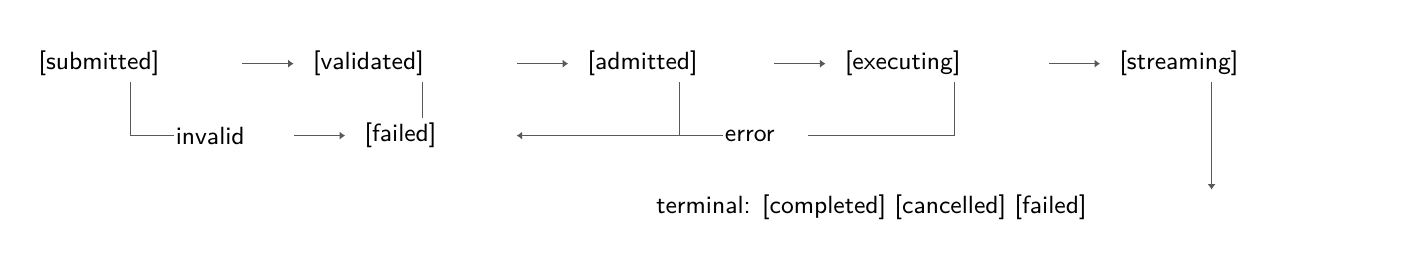
\begin{tikzpicture}[x=6.2pt,y=-13pt,draw=black!65,line width=.45pt]
\path[use as bounding box] (-1,-1) rectangle (79,5);
\draw (12,0) -- (11.5,0);
\draw (12,0) -- (12.5,0);
\draw (13,0) -- (12.5,0);
\draw (13,0) -- (13.5,0);
\draw[-{Latex[length=2pt,width=3pt]}] (13.5,0) -- (14.5,0);
\draw (28,0) -- (27.5,0);
\draw (28,0) -- (28.5,0);
\draw (29,0) -- (28.5,0);
\draw (29,0) -- (29.5,0);
\draw[-{Latex[length=2pt,width=3pt]}] (29.5,0) -- (30.5,0);
\draw (43,0) -- (42.5,0);
\draw (43,0) -- (43.5,0);
\draw (44,0) -- (43.5,0);
\draw (44,0) -- (44.5,0);
\draw[-{Latex[length=2pt,width=3pt]}] (44.5,0) -- (45.5,0);
\draw (59,0) -- (58.5,0);
\draw (59,0) -- (59.5,0);
\draw (60,0) -- (59.5,0);
\draw (60,0) -- (60.5,0);
\draw[-{Latex[length=2pt,width=3pt]}] (60.5,0) -- (61.5,0);
\node[anchor=west,inner sep=0pt,font=\sffamily\fontsize{9}{11}\selectfont] at (-0.4,0) {\begin{adjustbox}{max width=68.2pt}[submitted]\end{adjustbox}};
\node[anchor=west,inner sep=0pt,font=\sffamily\fontsize{9}{11}\selectfont] at (15.6,0) {\begin{adjustbox}{max width=68.2pt}[validated]\end{adjustbox}};
\node[anchor=west,inner sep=0pt,font=\sffamily\fontsize{9}{11}\selectfont] at (31.6,0) {\begin{adjustbox}{max width=62.0pt}[admitted]\end{adjustbox}};
\node[anchor=west,inner sep=0pt,font=\sffamily\fontsize{9}{11}\selectfont] at (46.6,0) {\begin{adjustbox}{max width=68.2pt}[executing]\end{adjustbox}};
\node[anchor=west,inner sep=0pt,font=\sffamily\fontsize{9}{11}\selectfont] at (62.6,0) {\begin{adjustbox}{max width=68.2pt}[streaming]\end{adjustbox}};
\draw (5,1) -- (5,0.5);
\draw (5,1) -- (5,1.5);
\draw (22,1) -- (22,0.5);
\draw (22,1) -- (22,1.5);
\draw (37,1) -- (37,0.5);
\draw (37,1) -- (37,1.5);
\draw (53,1) -- (53,0.5);
\draw (53,1) -- (53,1.5);
\draw (68,1) -- (68,0.5);
\draw (68,1) -- (68,1.5);
\draw (5,2) -- (5.5,2);
\draw (5,2) -- (5,1.5);
\draw (6,2) -- (5.5,2);
\draw (6,2) -- (6.5,2);
\draw (7,2) -- (6.5,2);
\draw (7,2) -- (7.5,2);
\draw (15,2) -- (14.5,2);
\draw (15,2) -- (15.5,2);
\draw (16,2) -- (15.5,2);
\draw (16,2) -- (16.5,2);
\draw[-{Latex[length=2pt,width=3pt]}] (16.5,2) -- (17.5,2);
\draw[-{Latex[length=2pt,width=3pt]}] (28.5,2) -- (27.5,2);
\draw (29,2) -- (28.5,2);
\draw (29,2) -- (29.5,2);
\draw (30,2) -- (29.5,2);
\draw (30,2) -- (30.5,2);
\draw (31,2) -- (30.5,2);
\draw (31,2) -- (31.5,2);
\draw (32,2) -- (31.5,2);
\draw (32,2) -- (32.5,2);
\draw (33,2) -- (32.5,2);
\draw (33,2) -- (33.5,2);
\draw (34,2) -- (33.5,2);
\draw (34,2) -- (34.5,2);
\draw (35,2) -- (34.5,2);
\draw (35,2) -- (35.5,2);
\draw (36,2) -- (35.5,2);
\draw (36,2) -- (36.5,2);
\draw (37,2) -- (36.5,2);
\draw (37,2) -- (37.5,2);
\draw (37,2) -- (37,1.5);
\draw (38,2) -- (37.5,2);
\draw (38,2) -- (38.5,2);
\draw (39,2) -- (38.5,2);
\draw (39,2) -- (39.5,2);
\draw (45,2) -- (44.5,2);
\draw (45,2) -- (45.5,2);
\draw (46,2) -- (45.5,2);
\draw (46,2) -- (46.5,2);
\draw (47,2) -- (46.5,2);
\draw (47,2) -- (47.5,2);
\draw (48,2) -- (47.5,2);
\draw (48,2) -- (48.5,2);
\draw (49,2) -- (48.5,2);
\draw (49,2) -- (49.5,2);
\draw (50,2) -- (49.5,2);
\draw (50,2) -- (50.5,2);
\draw (51,2) -- (50.5,2);
\draw (51,2) -- (51.5,2);
\draw (52,2) -- (51.5,2);
\draw (52,2) -- (52.5,2);
\draw (53,2) -- (52.5,2);
\draw (53,2) -- (53,1.5);
\draw (68,2) -- (68,1.5);
\draw (68,2) -- (68,2.5);
\node[anchor=west,inner sep=0pt,font=\sffamily\fontsize{9}{11}\selectfont] at (7.6,2) {\begin{adjustbox}{max width=43.4pt}invalid\end{adjustbox}};
\node[anchor=west,inner sep=0pt,font=\sffamily\fontsize{9}{11}\selectfont] at (18.6,2) {\begin{adjustbox}{max width=49.6pt}[failed]\end{adjustbox}};
\node[anchor=west,inner sep=0pt,font=\sffamily\fontsize{9}{11}\selectfont] at (39.6,2) {\begin{adjustbox}{max width=31.0pt}error\end{adjustbox}};
\draw[-{Latex[length=2pt,width=3pt]}] (68,2.5) -- (68,3.5);
\node[anchor=west,inner sep=0pt,font=\sffamily\fontsize{9}{11}\selectfont] at (35.6,4) {\begin{adjustbox}{max width=260.40000000000003pt}terminal: [completed] [cancelled] [failed]\end{adjustbox}};
\end{tikzpicture}
\end{adjustbox}\end{center}

Real engines add queued, blocked, preempted, draining, or model-loading
states. The minimum invariant is more important than the exact labels:

\begin{quote}
\textbf{FIRST PRINCIPLE} Every submitted generation reaches one
observable terminal outcome, and an admitted generation releases its
owned state exactly once.
\end{quote}

ENGINE-0 uses three terminal outcomes:

\begin{itemize}
\tightlist
\item
  \texttt{\seqsplit{Completed(StopReason)}} means generation stopped
  according to a successful rule. Its reason is \texttt{EndOfSequence}
  or \texttt{MaxTokens}.
\item
  \texttt{Cancelled} means the caller or control policy withdrew the
  work.
\item
  \texttt{\seqsplit{Failed(GenerationError)}} means invalid input, model
  failure, or an equivalent error prevented successful completion.
\end{itemize}

Cancellation is not successful completion. Failure is not cancellation.
A token limit and a model end marker are both successful stops but have
different causes. Keeping these distinctions internally allows a server
to map them to a wire protocol honestly.

The canonical
\href{https://github.com/hermonai/inside-the-llm-engine/blob/astra-visual-rewrite/diagrams/runtime/request-to-token.txt}{request-to-token
diagram} shows every terminal branch. Its most important line is at the
bottom: after a terminal event, no token or trace event may be emitted.
That sounds small. In a concurrent server it prevents duplicated close
chunks, usage reported twice, state released twice, and tokens arriving
after a client believes the answer is over.

\subsubsection{A stream is an ordered
contract}\label{a-stream-is-an-ordered-contract}

A stream is not ``some callbacks happen.'' It is a sequence of events
with ordering and termination semantics. ENGINE-0's public stream
contains zero or more token events followed by one terminal event. Its
sink is deliberately infallible so Chapter 1 can isolate the producer's
lifecycle. Later we will add bounded queues, backpressure, network
departure, and sink failure.

Token identity and output piece are also different. A tokenizer's
vocabulary token can correspond to a fragment whose bytes do not form a
complete Unicode string alone. Production runtimes may buffer bytes
across token boundaries before emitting valid text. Therefore, a wire
\emph{piece} need not correspond one-to-one with a token. ENGINE-0
prints one teaching piece per text token and states that limitation
explicitly.

\subsection{Latency is a distance between named
events}\label{latency-is-a-distance-between-named-events}

Saying ``latency is 120 milliseconds'' is incomplete. From which event
to which event? Under what concurrency? Does it include queueing, model
load, tokenization, network transfer, or client rendering?

Name lifecycle timestamps first: \(t_0\) when the request enters the
measured runtime boundary, \(t_a\) at admission, \(t_s\) when execution
starts, \(t_r\) when the first token is ready, \(t_e\) when its first
externally visible event is emitted, \(t_i\) for each later output
event, and \(t_T\) for the terminal event. All timestamps use one
monotonic clock.

The named endpoint differences are:

\[
\begin{aligned}
T_{\mathrm{queue}} &= t_s-t_a && [\mathrm{s}],\\
T_{\mathrm{first\ compute}} &= t_r-t_s && [\mathrm{s}],\\
T_{\mathrm{ready\to emit}} &= t_e-t_r && [\mathrm{s}],\\
T_{\mathrm{TTFT}} &= t_e-t_a && [\mathrm{s}],\\
T_{\mathrm{ITL},i} &= t_i-t_{i-1} && [\mathrm{s}],\\
T_{\mathrm{request}} &= t_T-t_0 && [\mathrm{s}].
\end{aligned}
\]

Some systems measure time to first token from client arrival rather than
admission. Some report the first token identity before complete text
bytes are available. Neither choice is universally wrong, but the
endpoints must travel with the number.

A useful conceptual decomposition for \(N_{\mathrm{decode}}\) decode
steps is:

\[
T_{\mathrm{total}}
=T_{\mathrm{network}}+T_{\mathrm{queue}}+T_{\mathrm{prepare}}
+T_{\mathrm{prefill}}
+\sum_{t=1}^{N_{\mathrm{decode}}}T_{\mathrm{decode},t}
+T_{\mathrm{stream}}.
\]

This is a sum of measured categories only if the implementation actually
records compatible boundaries. It is not permission to invent an
end-to-end number by adding unrelated benchmarks. Some terms may overlap
in a pipelined engine; in that case a timeline, not a simple sum, is the
truthful model. The canonical
\href{https://github.com/hermonai/inside-the-llm-engine/blob/astra-visual-rewrite/diagrams/runtime/latency-decomposition.txt}{latency
decomposition} keeps those endpoints visible.

\subsubsection{TTFT, ITL, and request latency answer different
questions}\label{ttft-itl-and-request-latency-answer-different-questions}

\textbf{Time to first token (TTFT)} describes how soon useful output
begins. \textbf{Inter-token latency (ITL)} describes the spacing of
later output. \textbf{Request latency} describes how long until the
request is terminal. A system can improve one and worsen another.
Waiting briefly to combine work may increase TTFT while improving
aggregate throughput. A long prompt can dominate TTFT even when later
decode steps are quick. A slow client can increase terminal latency
after the device has produced tokens.

Report distributions when many requests matter. An average can hide a
long tail caused by queueing, model cold starts, uneven output length,
or scheduling unfairness. Part XII will turn these names into
reproducible production measurement.

\subsubsection{Throughput is not the inverse of one request's
latency}\label{throughput-is-not-the-inverse-of-one-requests-latency}

Throughput is completed work per unit time. For a measurement interval
of \(\Delta t\) seconds:

\[
R_{\mathrm{request}}
=\frac{N_{\mathrm{completed\ requests}}}{\Delta t}
\quad[\mathrm{requests/s}],
\qquad
R_{\mathrm{token}}
=\frac{N_{\mathrm{emitted\ output\ tokens}}}{\Delta t}
\quad[\mathrm{tokens/s}].
\]

Both require a population and a workload definition. Requests with
different prompt and output lengths are not interchangeable work units.
Token throughput can hide poor fairness. Request throughput can hide
enormous differences in token count.

With concurrency greater than one, a system can increase total tokens
per second even if each request's token spacing gets slightly worse.
Conversely, a single request can have excellent latency while leaving
most hardware idle. That is why ``fast'' must be split into latency,
throughput, fairness, memory, and correctness rather than compressed
into one number.

\textbf{Concurrency} is the number of requests simultaneously admitted
or active. It is not automatically the size of one physical execution
batch. A scheduler may have ten admitted requests while executing
positions from only some of them in the next device call.

\subsection{Prefill and decode: a preview, not yet an
explanation}\label{prefill-and-decode-a-preview-not-yet-an-explanation}

Generation work changes shape over a request.

During \textbf{prefill}, the engine evaluates prompt positions and
creates reusable per-position state. There may be many prompt positions
available at once, so the numerical work can have substantial parallel
structure.

During \textbf{decode}, the engine advances active sequences with newly
generated positions. For an ordinary autoregressive sequence, each step
contributes a small number of new query positions while consulting an
expanding history. That changes arithmetic intensity, memory traffic,
batching opportunities, and latency sensitivity.

This distinction will become mathematical in Part IV. For Chapter 1,
retain only three facts:

\begin{enumerate}
\def\labelenumi{\arabic{enumi}.}
\tightlist
\item
  tokenization is not prefill;
\item
  prefill and decode use the same model parameters but present different
  work shapes to the runtime;
\item
  a scheduler may mix prompt and decode work from different requests in
  one physical execution step.
\end{enumerate}

ENGINE-0 has neither phase. Its \texttt{\seqsplit{Model::candidates}}
call is a lifecycle marker, not a claim to implement prefill or decode.

\subsection{``GPU inference'' still has a CPU and a
runtime}\label{gpu-inference-still-has-a-cpu-and-a-runtime}

A GPU can perform large numerical operations very effectively. That does
not mean the request bypasses host software.

Someone must accept and validate the request, tokenize or otherwise
prepare inputs, choose a device and execution plan, allocate or find
state, submit work, handle completion, apply some selection and stopping
policies, convert output to protocol events, and react to cancellation.
Different systems move more of these tasks onto devices or overlap them
with device work, but the control path remains.

NVIDIA's current TensorRT-LLM architecture, for example, documents a
high-level \texttt{LLM} interface that manages tokenization and creates
executor workers. Its \texttt{PyExecutor} coordinates a scheduler, model
engine, and decoder; its overlap scheduler can launch GPU work for one
step while processing previous results on the CPU
(\href{https://nvidia.github.io/TensorRT-LLM/latest/developer-guide/overview.html}{TensorRT-LLM
architecture overview}). The important lesson is not a claim that every
engine should copy that design. It is that CPU orchestration and GPU
execution can overlap and cooperate. The device is a backend
participant, not the owner of the entire request.

A GPU can also lose for a particular operation. Transfers, command
encoding, kernel launch, synchronization, small shapes, unsupported
layouts, and idle gaps can dominate useful arithmetic. We will measure
those crossovers in Part VIII. For now, reject two symmetrical myths:
``GPU means the whole request is on the GPU'' and ``CPU work means GPU
acceleration failed.''

\subsection{Current engines expose different
boundaries}\label{current-engines-expose-different-boundaries}

The system map is not invented from one codebase. Current official
sources show several valid decompositions.

\textbf{llama.cpp} exposes both a library and \texttt{llama-server}. Its
server developer documentation describes HTTP routes, thread-safe
request/response queues, a \texttt{server\_context} that owns primary
inference state, and per-sequence \texttt{server\_slot} objects. The
server advertises parallel decoding and continuous batching
(\href{https://github.com/ggml-org/llama.cpp/blob/3466812d1f06728effe7c0f3c0671117f461672d/tools/server/README-dev.md}{llama-server
developer documentation}).

\textbf{vLLM} offers an offline \texttt{LLM} entry point and online
serving. Its documented V1 topology separates API input/streaming,
engine-core scheduling and KV management, and device workers. This is a
clear example of the same engine role crossing process boundaries rather
than disappearing.

\textbf{SGLang} describes its runtime as combining continuous batching,
paged attention, prefix reuse, chunked prefill, and several parallel
execution forms. Its current scheduler source initializes model workers,
memory pools, request receivers, output streaming, scheduling policy,
and metrics. The safe Chapter 1 conclusion is bounded: a model worker is
one component inside a larger request-and-resource runtime. Feature
support for a particular model or device requires a later, narrower
audit
(\href{https://github.com/sgl-project/sglang/blob/221a6273ce3212c79483df233b4511fdf8fbe6d0/python/sglang/srt/managers/scheduler.py}{SGLang
scheduler at the inspected commit}).

\textbf{Hugging Face Transformers} provides
\texttt{\seqsplit{GenerationMixin.generate}}, generation configuration,
logits processors, stopping criteria, and streamer hooks. That is a
powerful library-level generation surface, but it is not by itself a
multi-client service
(\href{https://huggingface.co/docs/transformers/main_classes/text_generation}{Transformers
generation API}).

\textbf{Text Generation Inference (TGI)} shows a serving decomposition:
a Rust router/webserver receives and batches requests, a launcher starts
components, and one or more model servers perform inference behind gRPC.
Its official docs now mark TGI as maintenance mode and recommend current
engines including vLLM, SGLang, and local options such as llama.cpp. The
architecture is still useful, but the maintenance status belongs beside
any present-day recommendation
(\href{https://huggingface.co/docs/text-generation-inference/architecture}{TGI
architecture},
\href{https://huggingface.co/docs/text-generation-inference/index}{status
notice}).

These projects do not prove one universal class hierarchy. They support
a more durable claim: input processing, request control, model
execution, memory ownership, selection, and output streaming are
separable responsibilities even when a particular implementation
combines them.

\subsection{Inside Hermon: one verified current request
path}\label{inside-hermon-one-verified-current-request-path}

The canonical
\href{https://github.com/hermonai/inside-the-llm-engine/blob/astra-visual-rewrite/diagrams/runtime/hermon-current-request-path.txt}{source-status
path} summarizes the local and provider branches below; its labels apply
to the inspected commit, not to every Hermon revision.

Hermon is this book's recurring production case study. The following
account is \textbf{CURRENT} only for commit
\href{https://github.com/hermonai/hermon/commit/472a44cdb511b2dae6c9569e59543db8f8350b25}{\texttt{472a44c}},
inspected on 2026-09-03. The durable source record is in the
\href{https://github.com/hermonai/inside-the-llm-engine/blob/astra-visual-rewrite/research/part-01/chapter-01-the-missing-half-of-ai.md}{Chapter
1 research note}.

\begin{quote}
\textbf{INSIDE HERMON --- CURRENT} For an OpenAI-compatible request,
\texttt{hermon-api} first resolves the model name through its provider
router. In an engine-enabled binary, if the name also resolves to a
local GGUF and the native engine is linked, the handler calls
\texttt{\seqsplit{engine\_route::stream\_with\_options}}, then
\texttt{\seqsplit{hermon\_runtime::Dispatcher::stream\_with\_options}}.
Otherwise the inspected handler falls through to its Ollama client path.
\end{quote}

This is why provider and backend must remain separate in our vocabulary.
The provider router classifies a destination and connection information.
The local engine gate establishes whether this specific request can use
the in-process execution path. Tracing one without the other would
produce an incomplete claim.

The dispatcher reads \texttt{\seqsplit{HERMON\_RUNTIME\_MODE}} when it
is constructed. Unset and unrecognized values choose \texttt{batched}.
The dispatcher canonicalizes the model path, caches one per-model
runtime, and clones a short-lived \texttt{Arc} without holding the map
lock across inference.

\begin{quote}
\textbf{INSIDE HERMON --- CURRENT} The default \texttt{BatchedRuntime}
owns one shared llama.cpp model, one multi-sequence context, a
submission channel, one dedicated OS worker thread, and atomic metrics.
The worker alone mutates the context, shared batch, active-sequence
table, per-request samplers, and sticky-slot prefix metadata.
\end{quote}

The worker admits normalized sequence requests into logical slots. On
each iteration it assembles prompt chunks or pending decode positions
from active requests into one physical \texttt{llama\_batch}, calls
\texttt{decode\_batch}, samples the correct logit row for each eligible
sequence, buffers token bytes until it can emit valid UTF-8, and either
continues or finalizes. Sticky slots may retain a matching prompt prefix
in the same sequence slot. That is reuse, but it is not cross-request
physical page sharing.

At the lower runtime boundary, a successful stream is zero or more
\texttt{Piece(String)} values followed by exactly one
\texttt{\seqsplit{Done(EngineMetrics)}}, then channel close. An
\texttt{EngineError} receives no \texttt{Done}. The per-request output
channel is bounded, so a slow consumer eventually delays producer sends
instead of creating an unbounded output queue. Runtime metrics count
admissions, completions, failures, prefill/decode work, cache behavior,
speculation, active slots, and warm slots. The dispatcher's snapshot
endpoint includes batched runtimes; it does not pretend pool and paged
modes expose the same current metrics surface.

\begin{quote}
\textbf{INSIDE HERMON --- PREVIEW} Selecting
\texttt{\seqsplit{HERMON\_RUNTIME\_MODE=paged}} is explicit preview
behavior. Real packed-GGUF execution requires the additional
\texttt{\seqsplit{HERMON\_PAGED\_GGUF=1}} gate and remains CPU, greedy,
and serialized per model at the inspected commit.
\end{quote}

\begin{quote}
\textbf{INSIDE HERMON --- LIBRARY} Hermon's native kernel and
expert-storage components exist as usable, tested libraries, but their
existence does not mean they own the default request path. Default
execution still uses the pinned llama.cpp route through
\texttt{BatchedRuntime}.
\end{quote}

This status vocabulary prevents a common documentation failure: finding
a source file named \texttt{paged} or \texttt{cuda} and silently
describing it as the default runtime. Current means reached by the
verified default path. Preview means implemented behind a gate. Library
means a component exists without end-to-end default integration.

The source trace also preserved two caveats. The opening comment in
\texttt{dispatch.rs} still speaks from the older pool-era perspective
even though the executable default is batched. More importantly, the
lower runtime contract distinguishes error from successful
\texttt{Done}, while the inspected OpenAI SSE adapter logs an
engine-stream error, exits its receive loop, and then attempts a generic
\texttt{finish\_reason:\ stop} close and \texttt{{[}DONE{]}}. Chapter 1
does not repair Hermon, and this task did not authorize doing so. It
records the boundary so the later protocol chapter can audit whether
terminal cause survives every adapter.

\subsection{Build ENGINE-0}\label{build-engine-0}

We now need an executable system small enough to understand completely.
A real model would force us to explain tokenization, tensor math, model
files, and sampling before we could test the request lifecycle. Instead,
ENGINE-0 makes the model boundary artificial and the runtime boundary
real.

The workspace lives at
\href{https://github.com/hermonai/inside-the-llm-engine/blob/astra-visual-rewrite/code/mini-engine/README.md}{\texttt{\seqsplit{code/mini-engine}}}.
It is Rust 2021, forbids unsafe code, and has no external dependencies.

\begin{quote}
\textbf{BUILD IT} Run ENGINE-0 with its trace enabled:

\begin{verbatim}
cd code/mini-engine
cargo run -p engine0 -- --trace 'What color is the sky?'
\end{verbatim}
\end{quote}

The model-facing oracle has two tables. At step 0:

\begin{verbatim}
blue=9, green=4, <eos>=1
\end{verbatim}

At step 1:

\begin{verbatim}
<eos>=10, blue=1
\end{verbatim}

The greedy selector chooses the highest score. Therefore the semantic
output is one text token, \texttt{blue}, followed by successful
end-of-sequence. These integers are \textbf{not logits}. They are
candidate scores designed to be checked without neural-network
knowledge. The independent expected result is stored in
\href{https://github.com/hermonai/inside-the-llm-engine/blob/astra-visual-rewrite/code/reference/engine-0-oracle.md}{\texttt{\seqsplit{code/reference/engine-0-oracle.md}}}.

\subsubsection{The public concepts}\label{the-public-concepts}

\texttt{Request} contains a stable ID, opaque prompt text, and a
positive maximum number of new tokens. Validation rejects a blank prompt
or zero token budget. ENGINE-0 treats prompt text as opaque because
Chapter 2 owns tokenization.

\texttt{GenerationState} contains generated tokens and exposes the
current step. The runtime creates and mutates it. The model borrows it
for one candidate call but cannot emit events or finalize the request.

\texttt{Model} is a trait:

\begin{verbatim}
pub trait Model {
    fn candidates(
        &self,
        request: &Request,
        state: &GenerationState,
    ) -> Result<Vec<Candidate>, ModelError>;
}
\end{verbatim}

This is the substitution seam for Chapters 2--3. A later model can
interpret tokenized input and produce genuine numerical output without
owning admission, streaming, or terminal behavior.

\texttt{Selector} chooses one \texttt{Token} from candidates. ENGINE-0's
\texttt{GreedySelector} keeps the highest score and uses the first
candidate as a deterministic tie break. Chapter 4 will replace this
small policy with complete logit transforms, random-number ownership,
stochastic sampling, and stopping rules.

\texttt{TokenSink} receives ordered \texttt{StreamEvent} values:

\begin{verbatim}
pub enum StreamEvent {
    Token { request_id: u64, index: usize, token: Token },
    Terminal { request_id: u64, outcome: TerminalOutcome },
}
\end{verbatim}

The terminal event carries completed, cancelled, or failed.
End-of-sequence is selected but not emitted as text. That keeps a model
control token from appearing in the user-visible answer.

\subsubsection{The runtime loop}\label{the-runtime-loop}

\texttt{\seqsplit{Runtime::generate}} owns the transition order:

\begin{enumerate}
\def\labelenumi{\arabic{enumi}.}
\tightlist
\item
  create lifecycle and generation state;
\item
  validate the request, failing terminally if invalid;
\item
  record admission and execution start;
\item
  check cancellation;
\item
  check the maximum-token limit;
\item
  ask the model for candidates;
\item
  ask the selector for one token;
\item
  complete on end-of-sequence, or append and emit a text token;
\item
  repeat until one terminal outcome;
\item
  return \texttt{\seqsplit{GenerationResult}} with tokens, outcome, and
  timings.
\end{enumerate}

The model never receives the sink. The selector never mutates request
state. The sink never decides whether generation continues. These
restrictions make ownership visible.

An internal \texttt{Lifecycle} object is the only component allowed to
produce the terminal transition. Its \texttt{finish} method rejects a
second finish with \texttt{AlreadyTerminal}. Token and trace emission
check the terminal flag and do nothing after it is set. This is defense
in depth: normal control flow consumes the lifecycle into a result,
while focused unit tests deliberately attempt the forbidden transitions.

\subsubsection{Trace mode is an experiment, not a
benchmark}\label{trace-mode-is-an-experiment-not-a-benchmark}

Trace events include admission, execution start, model invocation, token
selection, token emission, and terminal. Each carries an elapsed
duration from entry to \texttt{generate}. A typical run resembles:

\begin{verbatim}
Admitted
ExecutionStarted
ModelInvoked(step=0)
TokenSelected(step=0, token_id=1)
TokenEmitted(index=0, token_id=1)
ModelInvoked(step=1)
TokenSelected(step=1, token_id=0)
Terminal(Completed(EndOfSequence))
\end{verbatim}

Your microseconds will differ. ENGINE-0 runs synchronously, prints to a
terminal, and performs almost no model work. The values are useful for
identifying boundaries, not comparing machines or engines. A terminal
print can itself dominate the fake computation.

\begin{quote}
\textbf{PERFORMANCE LAB} Use trace mode only to name
\texttt{queue\_delay}, \texttt{\seqsplit{time\_to\_first\_token}},
\texttt{\seqsplit{ready\_to\_emit\_delay}}, and total runtime. Do not
publish the resulting microseconds as an inference benchmark.
\end{quote}

Try the explicit non-success paths:

\begin{verbatim}
cargo run -p engine0 -- --trace --cancel-at 0 'cancel this request'
cargo run -p engine0 -- --trace --fail-at 1 'fail after one token'
\end{verbatim}

The injected failure exits nonzero. Both runs still produce one terminal
event. The cancellation emits no token when checked at step 0. The
step-1 model failure may follow the valid \texttt{blue} token, but it
cannot also report completed.

\subsection{Prove the lifecycle before adding a
model}\label{prove-the-lifecycle-before-adding-a-model}

ENGINE-0 has eleven tests: two focused unit tests for the internal
terminal guard and nine integration tests for public behavior.

The proof obligations are:

\begin{enumerate}
\def\labelenumi{\arabic{enumi}.}
\tightlist
\item
  the hand-computable oracle selects \texttt{blue}, then
  end-of-sequence;
\item
  the trace order matches admission, execution, model, selection,
  emission, and terminal causality;
\item
  a maximum-token stop is explicit;
\item
  cancellation produces one cancelled terminal;
\item
  blank input fails without admission or token emission;
\item
  an injected model failure cannot also complete;
\item
  an empty candidate set fails explicitly;
\item
  repeated identical runs have identical semantic streams;
\item
  a terminal event is last;
\item
  a second internal terminal transition is rejected;
\item
  token and trace emission are blocked after terminal.
\end{enumerate}

Run the full gate:

\begin{verbatim}
cd code/mini-engine
cargo fmt --all -- --check
cargo check --workspace --all-targets
cargo test --workspace
cargo clippy --workspace --all-targets -- -D warnings
\end{verbatim}

\begin{quote}
\textbf{PROVE IT} Correctness is the terminal state machine plus the
candidate oracle. Timing output is not part of semantic equality.
Repeated runs compare stream events, not elapsed durations.
\end{quote}

This separation matters. Determinism does not mean identical wall-clock
time. It means that under identical request, model source, selection
policy, and cancellation configuration, the semantic outcome is stable.

\subsection{Where the naive engine
fails}\label{where-the-naive-engine-fails}

ENGINE-0 is production-shaped in lifecycle but intentionally naive in
scope.

It serves one request synchronously. There is no admission queue,
fairness policy, physical batch, or concurrent mutation. Its queue delay
is only the distance between two local timestamps. A real server must
handle work that arrives while resources are occupied.

Its model source allocates a small vector of integer-scored candidates.
There is no vocabulary-scale score vector, tensor computation,
tokenizer, model artifact, or device. Treating those integers as real
logits would confuse the teaching boundary with the model we have not
built.

Its sink is infallible. A real bounded channel can fill. A network
client can disconnect. A protocol adapter can fail after some pieces
have been delivered. The engine then needs a precise rule for whether
the request is cancelled, failed, drained, or allowed to finish
off-wire.

Its cancellation source is a deterministic step predicate. Production
cancellation races with model execution, device queues, output emission,
and resource release. Exactly-once terminal behavior becomes harder when
several tasks can observe cancellation simultaneously.

It loads no artifact and selects no provider or backend. Those omissions
keep Chapter 1 honest, but they also mean ENGINE-0 cannot answer a real
prompt. The correct response is to extend its seams, not to stuff every
future subsystem into \texttt{\seqsplit{Runtime::generate}}.

\subsection{Common mistakes}\label{common-mistakes}

\subsubsection{``The model answered the
request''}\label{the-model-answered-the-request}

The model contributed candidate computation. The engine owned the
request, selection, stream, stopping, and cleanup. Collapsing those
owners makes failure analysis vague.

\subsubsection{``Inference is the opposite of
training''}\label{inference-is-the-opposite-of-training}

They are different operational regimes, not mirror images. Both can use
forward computation. Their mutable state, scheduling, reliability, and
external contracts differ.

\subsubsection{``A token is the text chunk I
saw''}\label{a-token-is-the-text-chunk-i-saw}

A token is a vocabulary identifier. Output protocols carry bytes or
strings, which may combine or split token boundaries. ENGINE-0 makes
them one-to-one for teaching and labels the simplification.

\subsubsection{``The model is on the GPU, so the CPU is not
involved''}\label{the-model-is-on-the-gpu-so-the-cpu-is-not-involved}

Device kernels are part of a wider control and data path. Host work,
transfer, launch, synchronization, token handling, and protocol work
still need owners.

\subsubsection{``More tokens per second means lower
latency''}\label{more-tokens-per-second-means-lower-latency}

Aggregate throughput and per-request latency are different measurements.
Concurrency can increase one while worsening the other.

\subsubsection{``The stream ended, so it
completed''}\label{the-stream-ended-so-it-completed}

A channel can close after success, cancellation, producer failure,
consumer departure, or process loss. A robust contract carries terminal
cause rather than inferring success from silence.

\subsubsection{``The source file exists, so the feature is
current''}\label{the-source-file-exists-so-the-feature-is-current}

Reachability matters. Hermon's paged and native components are valuable
evidence, but source presence does not make them the default request
path. Gates, runtime selection, fallbacks, and tests determine status.

\begin{quote}
\textbf{ENGINEERING FAILURE} A protocol adapter receives a runtime error
after streaming two pieces. It logs the error, breaks its loop, and
emits its ordinary successful close chunk. The runtime failed correctly,
but the wire contract lied. Terminal cause must be traced through every
boundary, not checked only at the model worker.
\end{quote}

\subsection{Exercises}\label{exercises}

\subsubsection{CHECK}\label{check}

\begin{enumerate}
\def\labelenumi{\arabic{enumi}.}
\tightlist
\item
  For each noun---artifact, running model, request state, provider,
  backend, stream, terminal---write whether it is primarily persistent
  data, immutable runtime data, mutable runtime data, policy, or an
  interface. Explain any noun that spans categories.
\item
  An API reports ``latency: 80 ms.'' List at least five plausible
  endpoint pairs that number might describe. Which one would you call
  TTFT?
\item
  A service completes 20 requests in one second, each with a different
  output length. What can you conclude from ``20 requests/s''? What can
  you not conclude about token throughput, fairness, or tail latency?
\item
  Why can two requests safely share model weights but not necessarily
  sampler or generation state?
\end{enumerate}

\subsubsection{BUILD}\label{build}

Complete
\href{https://github.com/hermonai/inside-the-llm-engine/blob/astra-visual-rewrite/labs/lab-01-generate-one-token-manually.md}{Lab
1 --- Generate One Token Manually}. Predict the token and trace from the
independent oracle before running ENGINE-0. Capture one successful, one
cancelled, and one failed stream.

Add a \texttt{RecordingSink} assertion that every token index is
contiguous from zero. Do not change the fake model to make the test
easy; test the public stream.

\subsubsection{BREAK}\label{break}

Temporarily change the step-0 \texttt{green} score from 4 to 12. Predict
the new token before running. Which test fails, and why is that failure
evidence that the oracle is independent of the implementation?

In a temporary local branch, remove the terminal guard from
\texttt{emit\_token} and make the unit test attempt emission after
\texttt{finish}. Observe the failure, then restore the invariant. Do not
commit the broken state.

\subsubsection{EXTEND}\label{extend}

Implement a second deterministic selector that chooses the lowest token
ID, regardless of score. Use it with the same \texttt{Runtime},
\texttt{Request}, \texttt{Model}, and \texttt{TokenSink}. Explain which
events change and which lifecycle invariants remain unchanged.

Sketch---but do not yet implement---a \texttt{Tokenizer} boundary for
Chapter 2. Identify input bytes, output token IDs, error behavior, and
ownership. Keep selection and terminal behavior out of that interface.

\subsection{What this chapter has not
explained}\label{what-this-chapter-has-not-explained}

We have named stages that remain black boxes.

We have not explained how text becomes token IDs, why token boundaries
can cut across familiar words or Unicode boundaries, or how special
tokens participate in prompts. That is Chapter 2.

We have not explained embeddings, hidden states, tensor shapes, learned
weights, or how a numerical model produces a score for each vocabulary
item. Chapter 3 builds the smallest model that can do so.

We have not defined real logits, probability normalization, temperature,
top-k, top-p, random seeds, stop sequences, or the complete
autoregressive feedback loop. Chapter 4 owns those semantics.

We have only previewed prefill and decode. We have not derived KV
caching, continuous batching, paged memory, prefix reuse, speculative
decoding, quantization, SIMD, accelerators, distributed execution, or
production protocols. Later parts introduce each only after its simpler
predecessor and failure mode are visible.

Finally, we have not claimed that ENGINE-0 is fast. Its trace is
instrumentation for learning event boundaries. Performance claims begin
only after correctness, workload, hardware, and measurement controls are
explicit.

\subsection{Summary}\label{summary}

An LLM answer is not produced by weights alone. A model artifact must
become a running model. An inference engine must turn a request into
owned mutable state, coordinate compute and memory, invoke model work,
select tokens, stream bytes, and produce one terminal outcome. A server
and service add protocol and operational contracts without replacing the
engine's responsibility.

The durable distinctions are:

\begin{itemize}
\tightlist
\item
  training updates model parameters; inference advances requests with
  normally immutable weights;
\item
  an artifact is persistent representation; a running model is ready to
  execute; an engine owns request-to-outcome behavior;
\item
  provider routing and hardware backend execution are separate
  decisions;
\item
  the control plane decides and accounts; the data plane moves and
  transforms inference bytes;
\item
  token identity, byte representation, and lifetime ownership are
  different journeys that must agree;
\item
  completed, cancelled, and failed are distinct terminal outcomes;
\item
  TTFT, ITL, request latency, throughput, and concurrency answer
  different questions;
\item
  prefill and decode are different workload phases, even though we have
  not yet derived them;
\item
  GPU execution remains part of a host-coordinated runtime;
\item
  current, preview, and library status require call-path evidence.
\end{itemize}

ENGINE-0 makes the lifecycle executable. Its fake model chooses
\texttt{blue} from a hand-computable table. Its real contribution is the
contract around that choice: validation, admission, state ownership,
deterministic selection, ordered token emission, cancellation, failure,
named timing points, and exactly one terminal.

\subsection{Next: from text to tokens}\label{next-from-text-to-tokens}

Chapter 2 replaces the first fake boundary. We will begin with bytes,
construct a tokenizer contract, distinguish vocabulary identity from
text display, and prove round trips and failure behavior. The request
state machine remains in place. By the end of that chapter, ENGINE-0
will no longer treat the prompt as opaque, but it will still use the
same runtime, stream, and terminal ownership established here.

\subsection{Primary references}\label{primary-references}

\begin{itemize}
\tightlist
\item
  Hermon source and architecture at commit
  \href{https://github.com/hermonai/hermon/commit/472a44cdb511b2dae6c9569e59543db8f8350b25}{\texttt{472a44c}}:
  \href{https://github.com/hermonai/hermon/blob/472a44cdb511b2dae6c9569e59543db8f8350b25/crates/hermon-runtime/src/dispatch.rs}{\texttt{dispatch.rs}},
  \href{https://github.com/hermonai/hermon/blob/472a44cdb511b2dae6c9569e59543db8f8350b25/crates/hermon-runtime/src/batched.rs}{\texttt{batched.rs}},
  \href{https://github.com/hermonai/hermon/blob/472a44cdb511b2dae6c9569e59543db8f8350b25/crates/hermon-runtime/src/metrics.rs}{\texttt{metrics.rs}},
  and
  \href{https://github.com/hermonai/hermon/blob/472a44cdb511b2dae6c9569e59543db8f8350b25/docs/CORE_ENGINE_ARCHITECTURE.md}{\texttt{\seqsplit{CORE\_ENGINE\_ARCHITECTURE.md}}}.
\item
  llama.cpp,
  \href{https://github.com/ggml-org/llama.cpp/blob/3466812d1f06728effe7c0f3c0671117f461672d/tools/server/README-dev.md}{\texttt{llama-server}
  architecture at \texttt{3466812}}.
\item
  vLLM,
  \href{https://docs.vllm.ai/en/latest/design/arch_overview/}{current
  architecture overview}, source snapshot
  \href{https://github.com/vllm-project/vllm/commit/80389cfedd5040e382d64a64b1782f66de1a38bf}{\texttt{80389cf}}.
\item
  SGLang,
  \href{https://github.com/sgl-project/sglang/blob/221a6273ce3212c79483df233b4511fdf8fbe6d0/python/sglang/srt/managers/scheduler.py}{\texttt{Scheduler}
  at \texttt{221a627}}.
\item
  NVIDIA TensorRT-LLM,
  \href{https://nvidia.github.io/TensorRT-LLM/latest/developer-guide/overview.html}{current
  architecture overview}, source snapshot
  \href{https://github.com/NVIDIA/TensorRT-LLM/commit/fcc84548ee6000530222600b33c4e733eaaf4de1}{\texttt{fcc8454}}.
\item
  Hugging Face Transformers,
  \href{https://huggingface.co/docs/transformers/main_classes/text_generation}{generation
  API} and
  \href{https://huggingface.co/docs/transformers/generation_strategies}{generation
  strategies}, source snapshot
  \href{https://github.com/huggingface/transformers/commit/ac3244569528944b9d5773cafea525cd8a8b63de}{\texttt{ac32445}}.
\item
  Hugging Face Text Generation Inference,
  \href{https://huggingface.co/docs/text-generation-inference/architecture}{architecture}
  and
  \href{https://huggingface.co/docs/text-generation-inference/index}{current
  maintenance notice}, source snapshot
  \href{https://github.com/huggingface/text-generation-inference/commit/b4adbf2f6e2e721280bd0ea5f91d70f7d033f5ed}{\texttt{b4adbf2}}.
\end{itemize}

\clearpage

\section{Chapter 2 --- From Text to
Tokens}\label{chapter-2-from-text-to-tokens}

\subsection{The model does not receive your
sentence}\label{the-model-does-not-receive-your-sentence}

Suppose two people send what appears to be the same request:

\begin{verbatim}
Explain why token boundaries matter.
\end{verbatim}

One client sends a raw completion string. Another sends a chat message
with the role \texttt{user}. One runtime normalizes the text; another
preserves every byte. One uses the vocabulary packaged with the model;
another accidentally loads a tokenizer with the same family name but a
different revision. All four paths produce valid arrays of integers.
Only some of those arrays are the input the model was trained to
interpret.

The model does not receive a sentence, a chat bubble, or a row of
visible characters. It receives \textbf{token IDs}. Each ID refers to
one entry in one finite, configured \textbf{vocabulary}. The conversion
from text to those IDs is \textbf{tokenization}, and it can include
Unicode normalization, whitespace rules, pre-tokenization, a
segmentation algorithm, byte fallback, and explicit insertion of control
identities. On the output side, generated IDs become byte pieces. Those
pieces may cut through a UTF-8 character, so a runtime sometimes has to
wait for several tokens before it can emit valid text.

This boundary is part of model semantics. If it is wrong, the numerical
model can execute every matrix multiplication correctly and still
receive the wrong sequence.

Chapter 1 made request ownership real while treating the prompt as
opaque. This chapter opens that first black box. We will distinguish
text, Unicode scalar values, bytes, and token IDs; derive byte-pair
encoding (BPE) by hand; separate BPE from SentencePiece's Unigram
algorithm; make special-token insertion explicit; serialize a tiny chat
correctly; and stream decoded bytes without producing malformed UTF-8.
Then we will evolve ENGINE-0 so tokenization is real while its model
remains deliberately fake.

Chapter 3 will replace that fake model with numerical inference. We do
not cross that boundary here.

\subsection{Four sequences can describe one visible
input}\label{four-sequences-can-describe-one-visible-input}

Begin with a small piece of text:

\begin{verbatim}
世🚀
\end{verbatim}

It is tempting to count two ``characters'' and move on. An inference
engine needs more precise units. The
\href{https://github.com/hermonai/inside-the-llm-engine/blob/astra-visual-rewrite/diagrams/tokenizer/text-unicode-bytes-tokens.txt}{text/Unicode/bytes/tokens
diagram} shows four:

\begin{verbatim}
visible text       Unicode scalars       UTF-8 bytes           token IDs
"世🚀"         ->  U+4E16 U+1F680   ->  E4 B8 96 F0 9F 9A 80 -> [x, y, z]
                     2 scalars                7 bytes            model-specific
\end{verbatim}

The visible text is what a renderer shows. A \textbf{Unicode code point}
is an integer position in the Unicode codespace. A \textbf{Unicode
scalar value} is a code point excluding the surrogate range reserved for
UTF-16. UTF-8 encodes each scalar value as one to four bytes. A
tokenizer then maps a configured transform of those bytes or text units
to vocabulary identifiers.

None of these boundaries has to match another.

The letter \texttt{é} can be one scalar value, U+00E9. It can also be
represented by the canonically equivalent sequence U+0065 LATIN SMALL
LETTER E followed by U+0301 COMBINING ACUTE ACCENT. A user may perceive
one grapheme in both cases, but the second representation has two scalar
values and three UTF-8 bytes. An emoji such as
\texttwemoji{1f469-1f3fd-200d-1f4bb} contains multiple scalar values: a
person, a skin-tone modifier, a zero-width joiner, and a laptop. A
renderer may present the sequence as one grapheme. A tokenizer may split
it into many IDs, sometimes in the middle of one scalar's UTF-8
encoding.

Use \emph{character} only when its meaning is genuinely unambiguous. At
system boundaries, name the unit: grapheme, scalar value, UTF-8 byte, or
token ID.

\begin{quote}
\textbf{FIRST PRINCIPLE} A token is an identity in a particular model
vocabulary. It is not necessarily a word, character, Unicode scalar
value, byte, or output string.
\end{quote}

This distinction immediately explains why token-count rules cannot be
derived from word count. Punctuation may have its own ID or join a
neighboring piece. A leading space may be part of a token. A common word
may be one ID while a rare spelling becomes many. Chinese text has no
obligation to follow space-delimited English boundaries. An emoji can
require several byte-fragment tokens.

\subsection{UTF-8 is a byte encoding, not
tokenization}\label{utf-8-is-a-byte-encoding-not-tokenization}

Unicode assigns scalar values. UTF-8 specifies how to encode those
values as bytes. Its leading byte determines the expected sequence
length:

\begin{verbatim}
0xxxxxxx                            one byte
110xxxxx 10xxxxxx                  two bytes
1110xxxx 10xxxxxx 10xxxxxx         three bytes
11110xxx 10xxxxxx 10xxxxxx 10xxxxxx four bytes
\end{verbatim}

Those bit shapes are not the whole validity rule. Overlong encodings are
forbidden. UTF-16 surrogate code points are not scalar values and cannot
be encoded as valid UTF-8. Values above U+10FFFF are invalid.
Continuation bytes must appear in the permitted positions. The exact
well-formed ranges are specified by the Unicode Standard and RFC 3629.

Rust's \texttt{str} guarantees valid UTF-8. That is useful for
application text, but a tokenizer/runtime boundary still benefits from
byte-oriented interfaces for three reasons.

First, byte-level vocabularies define pieces in terms of bytes. Second,
generated token pieces may not be valid UTF-8 independently. Third, a
low-level engine needs an explicit policy for arbitrary or malformed
bytes rather than letting a string conversion choose silently.

Our Chapter 2 tokenizer therefore accepts \texttt{\&{[}u8{]}} and
decodes token IDs to \texttt{\&{[}u8{]}}. A separate stream framer
interprets accumulated output as UTF-8. This does not claim that every
tokenizer API should expose raw bytes to every user. It keeps
representation and interpretation separate at the teaching boundary.

\subsubsection{Malformed bytes require
policy}\label{malformed-bytes-require-policy}

When bytes purport to be UTF-8, Unicode conformance treats ill-formed
sequences as an error condition; they cannot be interpreted as
characters. A product may signal an error, substitute U+FFFD REPLACEMENT
CHARACTER according to a documented maximal-subpart policy, or expose a
binary channel instead of a text channel. What it must not do is
accidentally mix policies.

ENGINE-0 uses a strict policy:

\begin{itemize}
\tightlist
\item
  when the buffer is valid or merely incomplete, emit its longest
  complete valid prefix and retain a suffix that later bytes could
  complete;
\item
  on a definitively invalid append, preserve the buffer and fail without
  emitting a new prefix from that append;
\item
  fail a would-be successful terminal if an incomplete suffix remains;
\item
  never perform lossy replacement.
\end{itemize}

This policy is especially useful for teaching because failure is
observable and raw pending bytes remain available for diagnostics.
Hermon's current production path chooses a different terminal behavior,
which we will inspect later.

\subsection{A tokenizer is a configured
pipeline}\label{a-tokenizer-is-a-configured-pipeline}

``The tokenizer uses BPE'' is not a complete tokenizer specification. A
useful pipeline model is:

\begin{verbatim}
input
  -> normalization
  -> pre-tokenization / boundary rules
  -> vocabulary model (BPE, Unigram, WordPiece, ...)
  -> special-token post-processing
  -> token IDs
\end{verbatim}

Decoding has its own configured inverse or cleanup steps. Hugging Face
Tokenizers exposes these responsibilities as normalizer, pre-tokenizer,
model, post-processor, and decoder components. Only the model component
is mandatory. That does not make the others unimportant; it means the
artifact must say which ones exist.

\subsubsection{Normalization}\label{normalization}

Unicode normalization can replace one valid scalar sequence with an
equivalent or compatibility-related sequence. NFC tends to compose; NFD
decomposes. NFKC and NFKD additionally apply compatibility mappings. A
tokenizer can instead choose identity normalization and preserve the
original sequence.

Other configured normalization may lowercase, strip accents, collapse
whitespace, add a dummy leading space, or replace spaces with a marker.
These are semantic transforms before vocabulary lookup. They can change
token IDs and destroy exact byte round trip.

Consider the composed and decomposed forms of \texttt{é}:

\begin{verbatim}
NFC-like input:  C3 A9
NFD-like input:  65 CC 81
\end{verbatim}

An identity tokenizer sees different bytes. An NFC-normalizing tokenizer
may make them equal before segmentation. Neither behavior is universally
correct. The model and tokenizer configuration determine the contract.

\subsubsection{Pre-tokenization}\label{pre-tokenization}

A pre-tokenizer introduces boundaries or transforms a stream into
regions the vocabulary model will process. It might separate
punctuation, isolate whitespace, use a regular expression, or map bytes
to a reversible visible alphabet. A BPE model usually does not merge
across a boundary it never sees.

This is one reason two byte-level BPE tokenizers can segment the same
text differently even if both cover all bytes. Their regular
expressions, byte mappings, vocabularies, and merge ranks can differ.

\subsubsection{Vocabulary model}\label{vocabulary-model}

The model component maps a region into vocabulary pieces and IDs. BPE
applies ranked merge rules. A Unigram model searches segmentations using
learned piece scores. WordPiece uses another greedy vocabulary
procedure. A word-level model may require a pre-tokenizer and map
unknown words to UNK.

The algorithm name still does not give an ID meaning. The exact
vocabulary artifact does.

\subsubsection{Post-processing and
decoding}\label{post-processing-and-decoding}

A post-processor can add BOS, EOS, separator, or classification tokens
after ordinary encoding. A decoder may reverse a byte mapping, turn a
metaspace symbol back into whitespace, remove continuation markers, or
perform cleanup. Exact round trip depends on the whole chain.

\begin{quote}
\textbf{PROVE IT} For every round-trip claim, state the domain and
configuration. ``All byte sequences round-trip through the toy
byte-fallback BPE with no normalization or special removal'' is
testable. ``Tokenization is reversible'' is too broad.
\end{quote}

\subsection{Vocabulary identity is model
identity}\label{vocabulary-identity-is-model-identity}

A vocabulary is a finite table. One direction associates IDs with token
definitions; the encoder uses enough additional structure to choose a
sequence of those IDs for input. Let \(V_{\mathrm{vocab}}\) be
vocabulary size and \(N\) be the number of token IDs in one encoded
input. Then every ordinary ID \(x_i\) must satisfy

\[
x_i\in\{0,1,\ldots,V_{\mathrm{vocab}}-1\},
\qquad 0\le i<N.
\]

This is the half-open code interval \texttt{0..V\_vocab} under the
vocabulary's indexing convention. But \texttt{id\ =\ 42} is not
portable. Vocabulary A may define 42 as bytes for a common word
fragment. Vocabulary B may assign 42 to punctuation, a byte fallback
piece, or a control identity.

The vocabulary also does not guarantee that every ID is ordinary text.
Some entries are controls. Some are unused. Some represent unknown
input. Some byte pieces do not form valid text alone.

This is why model loading eventually has to validate more than tensor
shapes. The artifact's weights learned relationships among positions
carrying these exact identities. Swapping a tokenizer changes the
meaning of the embedding row selected for each input position. We will
build embeddings in Chapter 3; for now, retain the contract: stable IDs
must reach that future lookup.

ENGINE-0 introduces a small \texttt{TokenId(u32)} newtype instead of
passing bare integers everywhere. The type cannot prove which vocabulary
an ID belongs to, but it prevents accidental arithmetic and makes
interfaces say when they carry identity rather than text.

\subsection{Build BPE from first
principles}\label{build-bpe-from-first-principles}

Byte-pair encoding appears in several tokenizer families, but the
essential encoding operation can be understood with five letters. Our
toy vocabulary starts with all 256 byte values, then adds learned merge
results.

The fixed merge table for \texttt{lower} is:

\begin{verbatim}
rank 0: l   + o   -> lo
rank 1: lo  + w   -> low
rank 2: e   + r   -> er
rank 3: low + er  -> lower
\end{verbatim}

The
\href{https://github.com/hermonai/inside-the-llm-engine/blob/astra-visual-rewrite/diagrams/tokenizer/bpe-merge-process.txt}{BPE
merge diagram} applies it:

\begin{verbatim}
bytes:        l | o | w | e | r
rank 0:      [l + o] -> lo       => lo | w | e | r
rank 1:     [lo + w] -> low      => low | e | r
rank 2:                    [e+r] => low | er
rank 3:             [low + er]  => lower
\end{verbatim}

The encoder starts from base symbols. It inspects adjacent pairs that
have merge rules, chooses the available rule with the lowest rank,
replaces that pair with the result symbol, and repeats until no rule
applies.

Two details matter.

First, these rules are fixed before the prompt arrives. BPE
\emph{training} learns a merge vocabulary from a corpus. BPE
\emph{encoding} applies the learned artifact. Counting pairs in a user's
prompt and inventing a merge would change the tokenizer during
inference.

Second, order is semantic. The result symbol of a later merge may
require an earlier result. Greedily choosing a visually large piece
without respecting ranks can produce a different segmentation. If the
same rank could apply at multiple positions, the toy contract chooses
the leftmost occurrence, then scans again. Production formats commonly
assign unique ranks to merge pairs, but occurrence order still needs
deterministic behavior.

\subsubsection{Hand cases}\label{hand-cases}

For \texttt{lolo}, rank 0 applies twice:

\begin{verbatim}
l | o | l | o
[l+o] | l | o -> lo | l | o
lo | [l+o]     -> lo | lo
\end{verbatim}

The result IDs are \texttt{{[}256,\ 256{]}} in our fixture.

For \texttt{xyz}, no merge rule applies. The result remains three base
byte IDs: \texttt{{[}120,\ 121,\ 122{]}}.

For empty input, the result is an empty ID vector. That is a valid
tokenizer result. The generation request layer may independently reject
an empty prompt. Keeping those decisions separate prevents a tokenizer
from owning API policy.

\subsubsection{A clarity-first
implementation}\label{a-clarity-first-implementation}

\texttt{\seqsplit{TinyBpeTokenizer}} stores the fixed rules and decoded
bytes for every merge result. Construction rejects duplicate pairs,
duplicate ranks, reserved result IDs, duplicate result IDs, and
references to symbols not defined by an earlier rule.

Encoding begins with one \texttt{TokenId} per byte. On every iteration
it scans all adjacent pairs, remembers the lowest-rank rule, merges one
occurrence, and repeats. This is deliberately easy to audit and can be
quadratic in input length. The limitation is part of the lesson. A
production tokenizer may use priority queues, linked symbol structures,
caching, vectorized search, or parallel pre-tokenization, but it must
preserve the configured segmentation.

\begin{quote}
\textbf{BUILD IT} Complete
\href{https://github.com/hermonai/inside-the-llm-engine/blob/astra-visual-rewrite/labs/lab-02-tokenize-by-hand.md}{Lab
2 --- Tokenize by Hand} before changing the merge table. Predict the
states for \texttt{lower}, \texttt{lolo}, and \texttt{xyz}, then compare
with the CLI.
\end{quote}

\subsection{Byte fallback is coverage, not
one-token-per-byte}\label{byte-fallback-is-coverage-not-one-token-per-byte}

Our toy starts with every byte, so any input byte sequence can be
represented. Known pairs can still merge into larger pieces.
\texttt{blue}, for example, follows \texttt{b+l\ -\textgreater{}\ bl},
\texttt{bl+u\ -\textgreater{}\ blu}, and
\texttt{blu+e\ -\textgreater{}\ blue}, becoming one ID in the toy
vocabulary. Unknown byte patterns remain base IDs.

This gives complete byte coverage without an ordinary unknown path. It
does not mean every input produces one token per byte. It also does not
mean the output is valid UTF-8. The byte sequence \texttt{C3\ 28} can
round-trip exactly through the tokenizer while remaining malformed as
UTF-8.

SentencePiece can optionally include 256 byte fallback pieces.
GPT-2-style byte-level BPE uses a reversible byte-to-Unicode alphabet
before applying BPE. These are related coverage strategies with
different representations. Neither phrase is sufficient to identify a
tokenizer.

OpenAI's GPT-2 reference encoder makes the layers visible. It encodes
input as UTF-8 bytes, maps all bytes to a reversible Unicode alphabet,
splits with a regular expression, applies ranked BPE, and maps pieces to
IDs. Decode performs the reverse vocabulary and byte mapping before
UTF-8 decoding. A token can therefore represent several original bytes,
and its byte fragment can be invalid UTF-8 alone.

\subsection{SentencePiece names a toolkit, not one
algorithm}\label{sentencepiece-names-a-toolkit-not-one-algorithm}

SentencePiece trains directly from raw sentences and packages
vocabulary, trainer settings, normalization, and other behavior in its
model artifact. It supports several model types. The two important ones
here are BPE and Unigram.

SentencePiece BPE applies a merge-based model. Its surrounding behavior
may use a dummy prefix and a metaspace marker such as \texttt{▁} to
represent word boundaries without assuming that spaces should disappear.

The SentencePiece Unigram model is different. It has a vocabulary of
candidate pieces with learned scores. Encoding searches for a
high-probability segmentation, commonly by dynamic programming. Training
starts with a larger candidate set and prunes pieces according to the
objective. There is no fixed ranked merge trace equivalent to our
\texttt{lower} example.

Calling both ``SentencePiece tokenization'' hides the algorithm
decision. A real engine must inspect the model type stored in the
artifact. It cannot dispatch to BPE merely because a file was produced
by SentencePiece.

\subsubsection{Unknown tokens and byte
fallback}\label{unknown-tokens-and-byte-fallback}

SentencePiece model configuration includes special pieces such as UNK,
BOS, EOS, and optionally PAD. Character coverage can leave rare input
outside the ordinary alphabet. Without byte fallback, such input can map
to UNK. That mapping loses information: decoding UNK cannot reconstruct
the original bytes.

With byte fallback enabled, out-of-vocabulary scalars can decompose into
UTF-8 byte pieces. This avoids ordinary unknown loss at the segmentation
stage. It does not reverse earlier normalization. If the normalizer
collapsed two spaces to one before fallback, the second space is already
gone.

\subsection{When does decode(encode(x)) equal
x?}\label{when-does-decodeencodex-equal-x}

Exact round trip is conditional. It can hold when:

\begin{itemize}
\tightlist
\item
  the input domain is covered without UNK loss;
\item
  normalization is identity or otherwise preserves the exact bytes in
  scope;
\item
  pre-tokenization uses a reversible representation;
\item
  decoding reverses every representation transform;
\item
  no special tokens are inserted, removed, or rendered differently;
\item
  no cleanup step changes spaces or punctuation.
\end{itemize}

It can fail when any of those conditions fails.

Our toy BPE has identity normalization, a complete byte alphabet,
reversible merges, and no implicit special insertion. Therefore, over
the domain \(\mathcal{B}^{*}\) of finite byte strings:

\[
\operatorname{decode}(\operatorname{encode}(\mathbf{x}))=\mathbf{x},
\qquad \mathbf{x}\in\mathcal{B}^{*}.
\]

The equality is over bytes. If \texttt{x} is malformed UTF-8, the result
is still the same malformed byte vector and cannot enter the text stream
successfully.

The real SentencePiece comparison later in this chapter demonstrates a
different configured contract. Its byte fallback covers the normalized
input, but its normalizer collapses or removes some whitespace. The
decoded surface is not the original source string for that fixture.

\subsection{Special tokens are control
identities}\label{special-tokens-are-control-identities}

The canonical
\href{https://github.com/hermonai/inside-the-llm-engine/blob/astra-visual-rewrite/diagrams/tokenizer/special-token-trust-boundary.txt}{special-token
trust boundary} separates untrusted surface text from
template-authorized control identities.

Model vocabularies commonly reserve identities with roles such as:

\begin{itemize}
\tightlist
\item
  \textbf{BOS}: beginning of sequence;
\item
  \textbf{EOS}: end of sequence or one configured end marker;
\item
  \textbf{PAD}: padding used to fill a shape or batch convention;
\item
  \textbf{UNK}: unknown input that could not be represented ordinarily;
\item
  role markers: system, user, assistant, tool, or model-specific roles;
\item
  end-of-turn or separator markers.
\end{itemize}

These names do not define universal IDs. BOS might be automatically
added for one model and forbidden for another. EOS may differ from an
end-of-turn marker. PAD must not automatically be treated as EOS. Some
models have several end-of-generation identities. UNK can be mandatory
even when a modern model rarely reaches it.

Special tokens also cross a trust boundary. Imagine a vocabulary with a
diagnostic spelling
\texttt{\textless{}\textbar{}assistant\textbar{}\textgreater{}}. If the
ordinary encoder automatically recognizes that byte string anywhere,
user content can inject the assistant control identity. The model then
sees a role transition that the structured request did not authorize.

ENGINE-0 prevents that structurally.
\texttt{\seqsplit{Tokenizer::encode(\&[u8])}} encodes ordinary data
only. It has no flag that turns marker-looking text into control IDs.
Trusted template output is a sequence of typed segments:

\begin{verbatim}
pub enum TemplateSegment {
    Text(Vec<u8>),
    Special(SpecialToken),
}
\end{verbatim}

\texttt{Text} goes through ordinary encoding. \texttt{Special} goes
through an explicit special-ID lookup. The string
\texttt{\textless{}\textbar{}assistant\textbar{}\textgreater{}} inside
\texttt{Text} remains its literal bytes. This separation makes the
authority visible in types and tests.

The toy assigns ordinary byte IDs \texttt{0..=255}, merge IDs beginning
at 256, and special IDs beginning at 1000. BOS, EOS, PAD, UNK, SYSTEM,
USER, ASSISTANT, and END\_TURN occupy distinct IDs. An ordinary decode
request for one of those control IDs returns a typed error instead of
pretending the diagnostic name is user text.

\begin{quote}
\textbf{FIRST PRINCIPLE} Ordinary text encoding and special-token
insertion are different operations with different authority.
\end{quote}

\subsection{A chat template is part of model
input}\label{a-chat-template-is-part-of-model-input}

A chat API presents messages as records:

\begin{verbatim}
role=system, content="Be concise."
role=user,   content="Why does this split?"
\end{verbatim}

A causal language model still receives one ID sequence. A \textbf{chat
template} serializes roles, content, separators, end-of-turn markers,
optional tool data, and the beginning of the generation turn according
to the convention used during training.

The
\href{https://github.com/hermonai/inside-the-llm-engine/blob/astra-visual-rewrite/diagrams/tokenizer/chat-template-pipeline.txt}{chat-template
diagram} shows the boundary:

\begin{verbatim}
[messages] --render--> [Text | Special segments] --encode/insert--> [token IDs]
\end{verbatim}

Our \texttt{\seqsplit{TinyChatTemplate}} is intentionally smaller than
production template languages:

\begin{verbatim}
BOS
SYSTEM encode(system content) END_TURN
USER   encode(user content)   END_TURN
ASSISTANT                       # when generation should begin
\end{verbatim}

The implementation accepts typed roles, not arbitrary strings. It
returns typed segments, not a marker-filled string that must later be
reparsed. That is enough to demonstrate the semantic owner without
embedding Jinja in the teaching engine.

\subsubsection{The wrong template can be valid
text}\label{the-wrong-template-can-be-valid-text}

A common fallback is:

\begin{verbatim}
system: Be concise.
user: Why does this split?
\end{verbatim}

Those bytes are valid UTF-8. The tokenizer can encode them. The request
can fit the context. The runtime can execute without error. Yet the IDs
contain no SYSTEM, USER, END\_TURN, or ASSISTANT controls from the tiny
model contract. Validity at the string or array layer does not establish
semantic correctness.

ENGINE-0 cannot measure the effect on answer quality because its model
still returns a fixed candidate table.
\href{https://github.com/hermonai/inside-the-llm-engine/blob/astra-visual-rewrite/labs/lab-04-use-the-wrong-chat-template.md}{Lab
4} therefore compares exact bytes and IDs, not generated quality. A
real-model quality claim would require a pinned model, correct baseline,
workload, and evaluation design.

\subsubsection{Raw completion is not chat
completion}\label{raw-completion-is-not-chat-completion}

A raw completion surface takes ordinary input intended to continue
directly. A chat completion surface first serializes structured
messages. Even when both contain the same visible user sentence, their
model inputs may differ by BOS, role headers, turn terminators,
assistant prefixes, and whitespace.

Do not automatically apply a chat template to raw input. Do not flatten
chat by intuition. The API surface selects a preparation contract.

\subsubsection{Avoid duplicate special
insertion}\label{avoid-duplicate-special-insertion}

Hugging Face's official chat-template guidance notes an important
failure mode. A template may already include BOS, EOS, or other
controls. If a caller renders the template to text and then tokenizes
with automatic special addition enabled, it can duplicate them.
Tokenizing through the template-aware surface is often safer because the
owner knows which controls are already present.

\texttt{\seqsplit{add\_generation\_prompt}} is also model-specific. For
templates that use an assistant-turn opener, it appends the sequence
that tells the model an assistant reply comes next. Some templates do
not need such a prefix. The flag does not define a universal string.

\subsection{Bind model, tokenizer, template, and special
semantics}\label{bind-model-tokenizer-template-and-special-semantics}

A directory containing \texttt{model.gguf}, \texttt{tokenizer.json}, and
a template file is not correct merely because every file parses. The
components must belong to the same model contract.

The
\href{https://github.com/hermonai/inside-the-llm-engine/blob/astra-visual-rewrite/diagrams/tokenizer/model-tokenizer-template-contract.txt}{contract
diagram} makes the dependency visible:

\begin{center}\begin{adjustbox}{max width=\linewidth}% Legacy topology preserved as native vectors and typeset labels.
\begin{tikzpicture}[x=6.2pt,y=-13pt,draw=black!65,line width=.45pt]
\path[use as bounding box] (-1,-1) rectangle (71,6);
\draw[-{Latex[length=2pt,width=3pt]}] (31.5,0) -- (30.5,0);
\draw (32,0) -- (31.5,0);
\draw (32,0) -- (32.5,0);
\draw (33,0) -- (32.5,0);
\draw (33,0) -- (33.5,0);
\draw[-{Latex[length=2pt,width=3pt]}] (33.5,0) -- (34.5,0);
\draw[-{Latex[length=2pt,width=3pt]}] (50.5,0) -- (49.5,0);
\draw (51,0) -- (50.5,0);
\draw (51,0) -- (51.5,0);
\draw (52,0) -- (51.5,0);
\draw (52,0) -- (52.5,0);
\draw[-{Latex[length=2pt,width=3pt]}] (52.5,0) -- (53.5,0);
\node[anchor=west,inner sep=0pt,font=\sffamily\fontsize{9}{11}\selectfont] at (7.6,0) {\begin{adjustbox}{max width=136.4pt}(tokenizer + revision)\end{adjustbox}};
\node[anchor=west,inner sep=0pt,font=\sffamily\fontsize{9}{11}\selectfont] at (35.6,0) {\begin{adjustbox}{max width=80.60000000000001pt}(special IDs)\end{adjustbox}};
\node[anchor=west,inner sep=0pt,font=\sffamily\fontsize{9}{11}\selectfont] at (54.6,0) {\begin{adjustbox}{max width=93.0pt}(chat template)\end{adjustbox}};
\draw (41,1) -- (41,0.5);
\draw (41,1) -- (41,1.5);
\node[anchor=west,inner sep=0pt,font=\sffamily\fontsize{9}{11}\selectfont] at (19.6,1) {\begin{adjustbox}{max width=266.6pt}╲                                         ╱\end{adjustbox}};
\draw (21,2) -- (21.5,2);
\draw (21,2) -- (21,1.5);
\draw (22,2) -- (21.5,2);
\draw (22,2) -- (22.5,2);
\draw (23,2) -- (22.5,2);
\draw (23,2) -- (23.5,2);
\draw (24,2) -- (23.5,2);
\draw (24,2) -- (24.5,2);
\draw (25,2) -- (24.5,2);
\draw (25,2) -- (25.5,2);
\draw (26,2) -- (25.5,2);
\draw (26,2) -- (26.5,2);
\draw (27,2) -- (26.5,2);
\draw (27,2) -- (27.5,2);
\draw (28,2) -- (27.5,2);
\draw (28,2) -- (28.5,2);
\draw (29,2) -- (28.5,2);
\draw (29,2) -- (29.5,2);
\draw (30,2) -- (29.5,2);
\draw (30,2) -- (30.5,2);
\draw (31,2) -- (30.5,2);
\draw (31,2) -- (31.5,2);
\draw (32,2) -- (31.5,2);
\draw (32,2) -- (32.5,2);
\draw (33,2) -- (32.5,2);
\draw (33,2) -- (33.5,2);
\draw (52,2) -- (51.5,2);
\draw (52,2) -- (52.5,2);
\draw (53,2) -- (52.5,2);
\draw (53,2) -- (53.5,2);
\draw (54,2) -- (53.5,2);
\draw (54,2) -- (54.5,2);
\draw (55,2) -- (54.5,2);
\draw (55,2) -- (55.5,2);
\draw (56,2) -- (55.5,2);
\draw (56,2) -- (56.5,2);
\draw (57,2) -- (56.5,2);
\draw (57,2) -- (57.5,2);
\draw (58,2) -- (57.5,2);
\draw (58,2) -- (58.5,2);
\draw (59,2) -- (58.5,2);
\draw (59,2) -- (59.5,2);
\draw (60,2) -- (59.5,2);
\draw (60,2) -- (60,1.5);
\node[anchor=west,inner sep=0pt,font=\sffamily\fontsize{9}{11}\selectfont] at (34.6,2) {\begin{adjustbox}{max width=99.2pt}exact identities\end{adjustbox}};
\draw (42,3) -- (42,2.5);
\draw (42,3) -- (42,3.5);
\draw[-{Latex[length=2pt,width=3pt]}] (42,3.5) -- (42,4.5);
\node[anchor=west,inner sep=0pt,font=\sffamily\fontsize{9}{11}\selectfont] at (33.6,5) {\begin{adjustbox}{max width=142.6pt}(running model weights)\end{adjustbox}};
\end{tikzpicture}
\end{adjustbox}\end{center}

ENGINE-0 introduces a small \texttt{ModelContract} that records:

\begin{itemize}
\tightlist
\item
  model identity;
\item
  tokenizer name and revision;
\item
  chat-template identity;
\item
  the tokenizer-owned special-ID mapping.
\end{itemize}

Before preparing chat input, it compares the concrete tokenizer and
template identities with the contract. This is not a full artifact
loader. It is a conceptual object that makes one failure explicit:
swapping only one semantic component is not a supported configuration.

Real systems need stronger provenance. A model repository revision,
hashes, embedded metadata, tokenizer assets, template revision, and
runtime support matrix may all participate. Part III will inspect model
containers and metadata. The invariant begins here.

\subsection{Generated tokens become bytes before they become
text}\label{generated-tokens-become-bytes-before-they-become-text}

On output, a model selects a token ID. The tokenizer vocabulary maps
that ID to a byte piece. Only the concatenation of pieces is expected to
represent output text.

The
\href{https://github.com/hermonai/inside-the-llm-engine/blob/astra-visual-rewrite/diagrams/tokenizer/token-to-byte-stream.txt}{token-to-stream
diagram} separates events and state:

\begin{center}\begin{adjustbox}{max width=\linewidth}% Legacy topology preserved as native vectors and typeset labels.
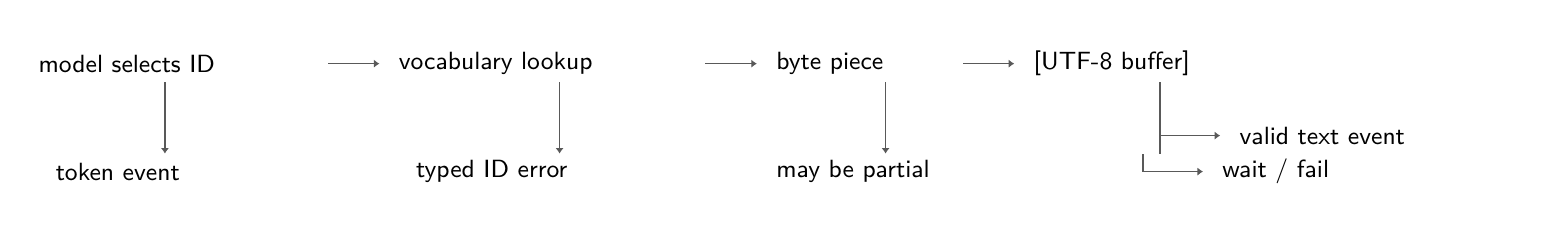
\begin{tikzpicture}[x=6.2pt,y=-13pt,draw=black!65,line width=.45pt]
\path[use as bounding box] (-1,-1) rectangle (87,4);
\draw (17,0) -- (16.5,0);
\draw (17,0) -- (17.5,0);
\draw (18,0) -- (17.5,0);
\draw (18,0) -- (18.5,0);
\draw[-{Latex[length=2pt,width=3pt]}] (18.5,0) -- (19.5,0);
\draw (39,0) -- (38.5,0);
\draw (39,0) -- (39.5,0);
\draw (40,0) -- (39.5,0);
\draw (40,0) -- (40.5,0);
\draw[-{Latex[length=2pt,width=3pt]}] (40.5,0) -- (41.5,0);
\draw (54,0) -- (53.5,0);
\draw (54,0) -- (54.5,0);
\draw (55,0) -- (54.5,0);
\draw (55,0) -- (55.5,0);
\draw[-{Latex[length=2pt,width=3pt]}] (55.5,0) -- (56.5,0);
\node[anchor=west,inner sep=0pt,font=\sffamily\fontsize{9}{11}\selectfont] at (-0.4,0) {\begin{adjustbox}{max width=99.2pt}model selects ID\end{adjustbox}};
\node[anchor=west,inner sep=0pt,font=\sffamily\fontsize{9}{11}\selectfont] at (20.6,0) {\begin{adjustbox}{max width=105.4pt}vocabulary lookup\end{adjustbox}};
\node[anchor=west,inner sep=0pt,font=\sffamily\fontsize{9}{11}\selectfont] at (42.6,0) {\begin{adjustbox}{max width=62.0pt}byte piece\end{adjustbox}};
\node[anchor=west,inner sep=0pt,font=\sffamily\fontsize{9}{11}\selectfont] at (57.6,0) {\begin{adjustbox}{max width=86.8pt}[UTF-8 buffer]\end{adjustbox}};
\draw (7,1) -- (7,0.5);
\draw (7,1) -- (7,1.5);
\draw (30,1) -- (30,0.5);
\draw (30,1) -- (30,1.5);
\draw (49,1) -- (49,0.5);
\draw (49,1) -- (49,1.5);
\draw (65,1) -- (65,0.5);
\draw (65,1) -- (65,1.5);
\draw[-{Latex[length=2pt,width=3pt]}] (7,1.5) -- (7,2.5);
\draw[-{Latex[length=2pt,width=3pt]}] (30,1.5) -- (30,2.5);
\draw[-{Latex[length=2pt,width=3pt]}] (49,1.5) -- (49,2.5);
\draw (65,2) -- (65,1.5);
\draw (65,2) -- (65.5,2);
\draw (65,2) -- (65,2.5);
\draw (66,2) -- (65.5,2);
\draw (66,2) -- (66.5,2);
\draw (67,2) -- (66.5,2);
\draw (67,2) -- (67.5,2);
\draw[-{Latex[length=2pt,width=3pt]}] (67.5,2) -- (68.5,2);
\node[anchor=west,inner sep=0pt,font=\sffamily\fontsize{9}{11}\selectfont] at (69.6,2) {\begin{adjustbox}{max width=99.2pt}valid text event\end{adjustbox}};
\draw (64,3) -- (64.5,3);
\draw (64,3) -- (64,2.5);
\draw (65,3) -- (64.5,3);
\draw (65,3) -- (65.5,3);
\draw (66,3) -- (65.5,3);
\draw (66,3) -- (66.5,3);
\draw[-{Latex[length=2pt,width=3pt]}] (66.5,3) -- (67.5,3);
\node[anchor=west,inner sep=0pt,font=\sffamily\fontsize{9}{11}\selectfont] at (0.6,3) {\begin{adjustbox}{max width=68.2pt}token event\end{adjustbox}};
\node[anchor=west,inner sep=0pt,font=\sffamily\fontsize{9}{11}\selectfont] at (21.6,3) {\begin{adjustbox}{max width=86.8pt}typed ID error\end{adjustbox}};
\node[anchor=west,inner sep=0pt,font=\sffamily\fontsize{9}{11}\selectfont] at (42.6,3) {\begin{adjustbox}{max width=86.8pt}may be partial\end{adjustbox}};
\node[anchor=west,inner sep=0pt,font=\sffamily\fontsize{9}{11}\selectfont] at (68.6,3) {\begin{adjustbox}{max width=68.2pt}wait / fail\end{adjustbox}};
\end{tikzpicture}
\end{adjustbox}\end{center}

Consider \texttt{世}, whose UTF-8 bytes are \texttt{E4\ B8\ 96}. Suppose
one generated ID maps to \texttt{E4\ B8} and the next maps to
\texttt{96}.

The first selection is a real token event. It advances generation
history and token accounting. It cannot produce a valid text event yet.
The buffer owns two pending bytes. The next token completes the scalar,
after which the runtime can emit \texttt{世} and clear the buffer.

The
\href{https://github.com/hermonai/inside-the-llm-engine/blob/astra-visual-rewrite/diagrams/tokenizer/utf8-partial-token-boundary.txt}{partial-boundary
diagram} shows the timeline:

\begin{verbatim}
token x bytes: E4 B8        [pending E4 B8]        text: (nothing)
token y bytes:       96  -> [pending E4 B8 96] -> validate -> text: "世"
\end{verbatim}

\subsubsection{The buffer has a small semantic
bound}\label{the-buffer-has-a-small-semantic-bound}

After every complete valid prefix is emitted, a valid incomplete UTF-8
suffix can contain at most three bytes: the beginning of a four-byte
scalar. That does not bound a network output queue or the number of
model tokens. It bounds this specific framing state.

\texttt{\seqsplit{Utf8StreamDecoder::push}} appends one piece and asks
Rust's UTF-8 validator for the status:

\begin{itemize}
\tightlist
\item
  complete valid buffer: emit it and clear;
\item
  error with no definite error length: emit the valid prefix, retain the
  incomplete suffix;
\item
  error with a definite error length: return \texttt{InvalidSequence}
  with the bytes.
\end{itemize}

\texttt{finish} succeeds only when no suffix remains. It never calls
\texttt{\seqsplit{String::from\_utf8\_lossy}}.

\subsubsection{Token latency and text latency can
differ}\label{token-latency-and-text-latency-can-differ}

Chapter 1 defined time to first token at an observable output boundary.
Now we can name two lower-level events:

\begin{verbatim}
first selected token ready
first valid text piece emitted
\end{verbatim}

They often occur close together for ASCII-heavy output. They can differ
when early token pieces are incomplete UTF-8 or non-rendered controls.
ENGINE-0 records both \texttt{\seqsplit{time\_to\_first\_token}} and
\texttt{\seqsplit{time\_to\_first\_text}}. These trace values remain
instructional, not benchmarks.

\begin{quote}
\textbf{BUILD IT} Complete
\href{https://github.com/hermonai/inside-the-llm-engine/blob/astra-visual-rewrite/labs/lab-03-stream-utf8-across-tokens.md}{Lab
3 --- Stream UTF-8 Across Token Boundaries}. Inject a partial scalar, a
definite malformed sequence, and an incomplete terminal suffix.
\end{quote}

\subsection{Evolve ENGINE-0 without building a second
runtime}\label{evolve-engine-0-without-building-a-second-runtime}

The Chapter 1 lifecycle remains:

\begin{verbatim}
validate -> admit -> execute -> select -> stream -> one terminal outcome
\end{verbatim}

The input and output boundaries become real:

\begin{verbatim}
input bytes -> tokenizer.encode -> Request.input_tokens
                                  |
                                  v
                         fake candidate model
                                  |
generated ID -> tokenizer.decode_token -> UTF-8 framer -> text stream
\end{verbatim}

The complete ownership map is stored in
\href{https://github.com/hermonai/inside-the-llm-engine/blob/astra-visual-rewrite/diagrams/tokenizer/engine0-token-ownership.txt}{\texttt{\seqsplit{engine0-token-ownership.txt}}}.

\texttt{Request} no longer owns an opaque prompt \texttt{String}. It
owns:

\begin{verbatim}
pub struct Request {
    pub id: RequestId,
    pub input_tokens: Vec<TokenId>,
    pub input_bytes: usize,
    pub max_new_tokens: usize,
}
\end{verbatim}

\texttt{input\_bytes} exists for trace/accounting context. The model
consumes IDs. Whitespace-only input is valid data now; an empty encoded
sequence is rejected by request validation. The tokenizer itself can
still encode empty bytes to an empty vector because that is the
mathematically correct transform.

\texttt{Token} now contains identity and kind, not a cached
\texttt{String}. This removes the Chapter 1 defect in which the fake
model effectively owned detokenized text. The tokenizer owns ID-to-byte
meaning.

\texttt{Runtime\textless{}M,\ S,\ T\textgreater{}} owns a model,
selector, and output tokenizer. After an ordinary token is selected, it:

\begin{enumerate}
\def\labelenumi{\arabic{enumi}.}
\tightlist
\item
  appends the identity to runtime-owned generation state;
\item
  emits the token identity event;
\item
  looks up the byte piece;
\item
  pushes the bytes into the request-local UTF-8 framer;
\item
  emits a text event only when a valid non-empty prefix exists;
\item
  continues or reaches one terminal outcome.
\end{enumerate}

EOS remains a control token. It is selected and traced but not decoded
as ordinary output. Before successful EOS or maximum-token completion,
the runtime verifies that the UTF-8 buffer is empty. A pending
incomplete suffix turns the attempted success into
\texttt{\seqsplit{Failed(Utf8Stream(...))}}. Cancellation and an earlier
model failure retain their own terminal causes; pending bytes are not
emitted after a non-success terminal.

\subsubsection{The fake model is still
fake}\label{the-fake-model-is-still-fake}

\texttt{DemoModel} returns the same hand-computable candidate ordering
as Chapter 1:

\begin{verbatim}
step 0: blue=9, green=4, EOS=1
step 1: EOS=10, blue=1
\end{verbatim}

The names now correspond to genuine vocabulary IDs whose byte pieces are
\texttt{blue} and \texttt{green}. The integer candidate scores are still
not logits. No embedding lookup, hidden vector, learned parameter,
output projection, or vocabulary-scale numerical result exists.

This distinction protects Chapter 3. We have made model input and output
representation real without pretending the source of candidate scores is
real.

\subsubsection{CLI probes}\label{cli-probes}

The executable keeps generation and adds two narrow probes:

\begin{verbatim}
cd code/mini-engine
cargo run -p engine0 -- tokenize lower
cargo run -p engine0 -- decode 259
cargo run -p engine0 -- --trace 'What color is the sky?'
\end{verbatim}

\texttt{tokenize} prints tokenizer identity, byte/scalar/token counts,
IDs, and piece bytes. \texttt{decode} accepts numeric ordinary IDs,
prints each byte piece, and runs the strict UTF-8 framer. The generation
trace adds \texttt{InputEncoded}, \texttt{TokenDecoded},
\texttt{Utf8Buffered}, and \texttt{TextEmitted} stages to the Chapter 1
lifecycle events.

The CLI is a teaching surface, not a standard tokenizer file format or
production protocol.

\subsection{Prove tokenization
independently}\label{prove-tokenization-independently}

The implementation is not its own oracle. Chapter 2 has three small
committed fixture groups under
\texttt{\seqsplit{code/mini-engine/fixtures/tokenizer/}} and a prose
oracle under \texttt{code/reference/}:

\begin{itemize}
\tightlist
\item
  the BPE rank table and hand encodings;
\item
  byte fragments for valid, malformed, and incomplete UTF-8;
\item
  the tiny chat-template control order.
\end{itemize}

The byte tokenizer is also an independent executable oracle for raw byte
round trips. It maps each byte directly to the numerically equal ID and
does not share the BPE merge algorithm.

The test suite covers four layers.

\subsubsection{Tokenizer semantics}\label{tokenizer-semantics}

\begin{itemize}
\tightlist
\item
  empty, ASCII, Chinese, emoji, combining, whitespace, repeated, and
  arbitrary malformed byte inputs;
\item
  deterministic encoding and exact byte round trip for the toy BPE;
\item
  merge prerequisites, rank order, leftmost repeat behavior, and
  unmergeable inputs;
\item
  invalid IDs and invalid merge tables;
\item
  ordinary marker-looking text versus explicit special insertion.
\end{itemize}

\subsubsection{Template and binding
semantics}\label{template-and-binding-semantics}

\begin{itemize}
\tightlist
\item
  exact BOS/role/end-turn/assistant control placement;
\item
  optional generation prompt;
\item
  marker-looking user content remains ordinary;
\item
  naive flattening produces different IDs;
\item
  mismatched tokenizer identity fails before preparation.
\end{itemize}

\subsubsection{UTF-8 framing semantics}\label{utf-8-framing-semantics}

\begin{itemize}
\tightlist
\item
  partial scalars across token boundaries;
\item
  several complete scalars in one piece;
\item
  valid prefix plus incomplete suffix;
\item
  definite malformed input;
\item
  incomplete terminal suffix;
\item
  empty pieces never create meaningless empty text events.
\end{itemize}

\subsubsection{Lifecycle integration}\label{lifecycle-integration}

\begin{itemize}
\tightlist
\item
  the \texttt{blue} then EOS oracle remains stable;
\item
  token and text events are separate and ordered;
\item
  cancellation, model failure, tokenizer failure, malformed output, and
  incomplete output each have one terminal;
\item
  no token, text, or trace event follows terminal;
\item
  repeated semantic streams agree with timing excluded.
\end{itemize}

Run the gate:

\begin{verbatim}
cd code/mini-engine
cargo fmt --all -- --check
cargo check --workspace --all-targets
cargo test --workspace
cargo clippy --workspace --all-targets -- -D warnings
\end{verbatim}

\subsection{Compare two real tokenizers without ranking
them}\label{compare-two-real-tokenizers-without-ranking-them}

Toy fixtures establish correctness, but real tokenizers show how much
the configured artifact matters. The durable experiment record is
\href{https://github.com/hermonai/inside-the-llm-engine/blob/astra-visual-rewrite/research/part-01/tokenizer-comparison.md}{\texttt{\seqsplit{research/part-01/tokenizer-comparison.md}}}.

It compares:

\begin{enumerate}
\def\labelenumi{\arabic{enumi}.}
\tightlist
\item
  OpenAI \texttt{tiktoken} 0.14.0, named encoding \texttt{cl100k\_base};
\item
  SentencePiece 0.2.2 with Google's pinned small Japanese BPE
  byte-fallback test model.
\end{enumerate}

The SentencePiece artifact is intentionally labeled as a test fixture,
not a production LLM tokenizer. The comparison observes counts and
pieces. It makes no speed or quality claim.

{\def\LTcaptype{none} % do not increment counter
\begin{longtable}[]{@{}
  >{\raggedright\arraybackslash}p{(\linewidth - 8\tabcolsep) * \real{0.30}}
  >{\raggedleft\arraybackslash}p{(\linewidth - 8\tabcolsep) * \real{0.14}}
  >{\raggedleft\arraybackslash}p{(\linewidth - 8\tabcolsep) * \real{0.12}}
  >{\raggedleft\arraybackslash}p{(\linewidth - 8\tabcolsep) * \real{0.20}}
  >{\raggedleft\arraybackslash}p{(\linewidth - 8\tabcolsep) * \real{0.24}}@{}}
\toprule\noalign{}
\begin{minipage}[b]{\linewidth}\raggedright
Input
\end{minipage} & \begin{minipage}[b]{\linewidth}\raggedleft
UTF-8 bytes
\end{minipage} & \begin{minipage}[b]{\linewidth}\raggedleft
Scalars
\end{minipage} & \begin{minipage}[b]{\linewidth}\raggedleft
\texttt{cl100k\_base}
\end{minipage} & \begin{minipage}[b]{\linewidth}\raggedleft
SentencePiece fixture
\end{minipage} \\
\midrule\noalign{}
\endhead
\bottomrule\noalign{}
\endlastfoot
\texttt{Tokenizers\ count\ spaces.} & 24 & 24 & 5 & 25 \\
two-line C-like loop & 39 & 39 & 21 & 38 \\
\texttt{模型把文本变成编号。} & 30 & 10 & 10 & 19 \\
\texttwemoji{1f469-1f3fd-200d-1f4bb}\texttwemoji{1f680} & 19 & 5 & 13 &
20 \\
whitespace/newline fixture & 34 & 34 & 9 & 30 \\
\end{longtable}
}

The numbers are not a scoreboard. The small SentencePiece vocabulary was
trained on a different corpus and has different normalization. Its
behavior is useful precisely because the setup is unlike
\texttt{cl100k\_base}.

\subsubsection{Pieces can cross scalar
boundaries}\label{pieces-can-cross-scalar-boundaries}

For the Chinese input, \texttt{cl100k\_base} splits the UTF-8 bytes of
\texttt{把} across two tokens: one piece contains \texttt{E6\ 8A}; the
next contains \texttt{8A}. Neither is valid UTF-8 alone. The
SentencePiece model uses byte fallback for several Chinese scalars. Both
reconstruct the input after complete byte concatenation.

For \texttwemoji{1f469-1f3fd-200d-1f4bb}\texttwemoji{1f680},
\texttt{cl100k\_base} produces 13 tokens. Many pieces are fragments such
as \texttt{F0\ 9F}, \texttt{91}, and \texttt{A9}. The SentencePiece
fixture produces a dummy metaspace boundary plus one fallback token per
emoji byte, for 20 tokens. This is the production-shaped reason for the
UTF-8 buffer, not an artificial corner case.

\subsubsection{Normalization can defeat exact surface round
trip}\label{normalization-can-defeat-exact-surface-round-trip}

The whitespace fixture contains leading spaces, a tab, two internal
spaces, a newline, and trailing spaces. \texttt{cl100k\_base} preserves
the exact surface in this experiment. The SentencePiece fixture decodes:

\begin{verbatim}
leading and internal trailing
\end{verbatim}

Its configured normalization removed and collapsed whitespace. Byte
fallback did not restore the original because fallback operated after
normalization. The two-line code input similarly decodes as one
normalized line under this fixture.

This is why a tokenizer contract includes normalization and decoding,
not only the subword algorithm.

\subsection{Token count is a systems
variable}\label{token-count-is-a-systems-variable}

Tokenization is model semantics, but token count also enters system
economics. If an encoded prompt has length \(N\), later stages see \(N\)
positions, not the number of words or bytes the caller expected.

For a model context capacity \(T_{\max}\) and requested generation
budget \(N_{\mathrm{new}}\), admission must at least respect the
dimensional constraint

\[
N+N_{\mathrm{new}}\le T_{\max}\quad[\mathrm{token\ positions}].
\]

Token count affects:

\begin{itemize}
\tightlist
\item
  whether input fits the model's context limit;
\item
  how much prefill work Chapter 20 will analyze;
\item
  how much per-position KV state later chapters allocate;
\item
  prefix/cache matching in token space;
\item
  maximum-generation and stop accounting;
\item
  batching shapes and admission budgets;
\item
  provider billing when tokens are the accounting unit;
\item
  rate limits and observability labels.
\end{itemize}

Do not turn this list into a premature performance formula. Different
model architectures, batching, hardware, and token distributions change
costs. The durable statement is dimensional: the engine schedules token
positions, so the correct tokenizer's \(N\) is an input to later work
and memory models. The canonical
\href{https://github.com/hermonai/inside-the-llm-engine/blob/astra-visual-rewrite/diagrams/tokenizer/token-count-system-impact.txt}{system-impact
map} shows those downstream dependencies without inventing a cost
coefficient.

A tokenizer with fewer tokens for one sentence is not automatically
better. Vocabulary size \texttt{V} also affects future embedding and
output dimensions. A larger vocabulary can reduce sequence length for
some inputs while increasing parameter rows and changing training
behavior. Language coverage and segmentation quality matter. We have not
measured any end-to-end tradeoff here.

\subsubsection{Cache boundaries use IDs, not reconstructed
text}\label{cache-boundaries-use-ids-not-reconstructed-text}

Two text surfaces that render identically after normalization may have
different original bytes. Two tokenizers can produce different ID
sequences for the same bytes. Prefix reuse in a model runtime must
compare the identities used for model state, not a casually re-rendered
string.

Hermon's current batched runtime tokenizes before choosing its best
prefix slot because the reusable state corresponds to token positions.
Its separate \texttt{\seqsplit{hermon-tokenizer}} crate sketches a
tokenizer prefix cache, but that crate does not own the current
real-model route.

\subsection{Inside Hermon: pinned llama.cpp owns the current
path}\label{inside-hermon-pinned-llama.cpp-owns-the-current-path}

The following account is \textbf{CURRENT} for Hermon commit
\href{https://github.com/hermonai/hermon/commit/472a44cdb511b2dae6c9569e59543db8f8350b25}{\texttt{472a44c}},
inspected on 2026-09-02. The detailed evidence is in the
\href{https://github.com/hermonai/inside-the-llm-engine/blob/astra-visual-rewrite/research/part-01/chapter-02-from-text-to-tokens.md}{Chapter
2 research note}.

The Hermon repository pins llama.cpp submodule commit
\href{https://github.com/ggml-org/llama.cpp/commit/389ff61d77b5c71cec0cf92fe4e5d01ace80b797}{\texttt{389ff61}}.
The upstream llama.cpp head observed during the inspection was newer.
Pinned does not mean stale by itself, and CURRENT does not mean ``equal
to upstream HEAD.'' It means that this pinned source owns the reachable
production path we traced.

\begin{quote}
\textbf{INSIDE HERMON --- CURRENT} The default \texttt{BatchedRuntime}
constructs a message view, asks the llama.cpp model wrapper to apply the
model's embedded chat template with an assistant generation prompt, and
uses a naive role flattener only when no embedded template exists. It
then calls context tokenization with special addition and special
parsing enabled.
\end{quote}

The Rust safe wrapper in
\texttt{\seqsplit{hermon-llamacpp/src/linked.rs}} crosses a narrow C
shim. The shim gets the model's llama.cpp vocabulary and calls
\texttt{llama\_tokenize}. The two Boolean controls matter: llama.cpp
documents \texttt{add\_special} as allowing configured BOS/EOS addition
and \texttt{parse\_special} as allowing control-token spellings to be
recognized instead of treated as plaintext.

Hermon's blocking raw stream calls the same tokenizer with
\texttt{\seqsplit{parse\_special=false}}. Its chat path first applies a
trusted template, then uses true. This is the same authority distinction
our typed teaching segments make, expressed through the pinned upstream
API.

\begin{quote}
\textbf{INSIDE HERMON --- LIBRARY}
\texttt{\seqsplit{crates/hermon-tokenizer}} currently defines a
tokenizer-kind enum, a \texttt{Tokenize} trait, and a prefix-cache
skeleton. Its own source labels BPE, SentencePiece, Tiktoken, and
Hugging Face ingestion as future work. Repository search found no
current real-model request route using it.
\end{quote}

Calling that crate ``Hermon's tokenizer'' without the status would be
misleading. The real-model owner today is the pinned llama.cpp
vocabulary path. The crate is a LIBRARY/research surface.

\subsubsection{Hermon's UTF-8 buffer}\label{hermons-utf-8-buffer}

Each active batched sequence owns
\texttt{utf8\_buf:\ Vec\textless{}u8\textgreater{}}. After sampling, the
worker calls \texttt{token\_to\_piece(token,\ false)}, appends the
resulting bytes, finds the longest prefix accepted by Rust's UTF-8
validator, emits that prefix as a
\texttt{\seqsplit{StreamItem::Piece(String)}}, and retains the rest.
This is direct production evidence that piece and token boundaries
differ.

The current implementation has a bounded caveat.

\begin{quote}
\textbf{INSIDE HERMON --- CURRENT CAVEAT} The buffer path uses
\texttt{valid\_up\_to()} without separately testing whether
\texttt{error\_len()} identifies a definite malformed sequence. At
successful finalization it converts leftover bytes with
\texttt{\seqsplit{String::from\_utf8\_lossy}}.
\end{quote}

Therefore Hermon's current policy does not match ENGINE-0's strict error
policy. A malformed suffix can remain buffered, and an incomplete or
invalid terminal suffix is rendered with replacement rather than
becoming an explicit runtime error. The blocking convenience engine has
a similar lossy terminal flush.

This chapter records the behavior; it does not modify Hermon. Later
production streaming and protocol chapters must decide the desired
policy, test it at the runtime boundary, and trace terminal cause to the
wire.

\subsubsection{What tests establish}\label{what-tests-establish}

Hermon's ignored real-model tests exercise tokenization, chat-template
application, token-to-piece concatenation, and next-token differential
behavior when an external model fixture and linked backend are supplied.
They establish useful model-dependent evidence when run. Ordinary CI
without the fixture does not prove every tokenizer/model combination.

The inspected default path has no focused unit test separating
valid-incomplete from definitively malformed UTF-8 fragments. ENGINE-0's
tests are evidence for the teaching contract, not retroactive proof of
Hermon.

\subsection{Common mistakes}\label{common-mistakes-1}

\subsubsection{``A token is a word''}\label{a-token-is-a-word}

Tokens can contain a whole word, a prefix, punctuation, a leading space,
many bytes, or an incomplete scalar fragment. Use vocabulary identity as
the definition.

\subsubsection{``UTF-8 characters are
tokens''}\label{utf-8-characters-are-tokens}

UTF-8 encodes scalar values into bytes. Tokenization is a separate
configured mapping. A tokenizer can split within the byte encoding of
one scalar.

\subsubsection{``SentencePiece means
Unigram''}\label{sentencepiece-means-unigram}

SentencePiece supports Unigram, BPE, word, and character model types.
Inspect the serialized model configuration.

\subsubsection{``Byte fallback guarantees exact input round
trip''}\label{byte-fallback-guarantees-exact-input-round-trip}

It guarantees coverage of bytes presented to the vocabulary model.
Earlier normalization can already have changed whitespace or scalar
sequences.

\subsubsection{``Decode each token as a
string''}\label{decode-each-token-as-a-string}

An individual piece may be invalid UTF-8. Decode to bytes, buffer per
request, and emit only complete valid prefixes under a named
malformed-data policy.

\subsubsection{``The marker string is the special
token''}\label{the-marker-string-is-the-special-token}

The control identity is the token. A printed marker is a diagnostic
surface. Ordinary user bytes that resemble it must not gain control
authority implicitly.

\subsubsection{``Any chat formatting is close
enough''}\label{any-chat-formatting-is-close-enough}

The template defines exact model input. A plausible
\texttt{role:\ content} string can be syntactically valid and
semantically wrong.

\subsubsection{``Add BOS and EOS everywhere for
safety''}\label{add-bos-and-eos-everywhere-for-safety}

Templates and tokenizer post-processors may already insert required
controls. Duplication changes the sequence. Follow the bound model
contract.

\subsubsection{``Fewer tokens is always
better''}\label{fewer-tokens-is-always-better}

Token count affects work, but vocabulary size, language coverage,
learned semantics, model compatibility, and workload also matter. Counts
from unrelated tokenizers are not a quality leaderboard.

\begin{quote}
\textbf{ENGINEERING FAILURE} A service loads weights from revision A and
a tokenizer/template from revision B. Every file parses and all token
IDs are in range. The model emits poor or strangely terminated output.
The defect is not numerical: the same integers select different learned
vocabulary rows and the role controls no longer match training. Artifact
identity must bind the components before execution.
\end{quote}

\subsection{Exercises}\label{exercises-1}

\subsubsection{CHECK}\label{check-1}

\begin{enumerate}
\def\labelenumi{\arabic{enumi}.}
\tightlist
\item
  For \texttt{é} written as U+0065 U+0301, count visible graphemes,
  scalar values, UTF-8 bytes, and tokens under the toy BPE. Repeat after
  NFC composition.
\item
  Explain why byte vectors can round-trip through
  \texttt{\seqsplit{TinyBpeTokenizer}} even when they cannot enter
  \texttt{\seqsplit{Utf8StreamDecoder}} successfully.
\item
  Classify BOS, EOS, PAD, UNK, USER, and END\_TURN as ordinary content,
  controls, or information-loss markers. Which names can share behavior
  only if model metadata says so?
\item
  A prompt has 1,000 Unicode scalar values and 1,600 tokens. Which count
  enters a 1,200-token context limit? What additional model/runtime
  facts are needed to estimate memory or latency?
\end{enumerate}

\subsubsection{BUILD}\label{build-1}

Complete
\href{https://github.com/hermonai/inside-the-llm-engine/blob/astra-visual-rewrite/labs/lab-02-tokenize-by-hand.md}{Lab
2},
\href{https://github.com/hermonai/inside-the-llm-engine/blob/astra-visual-rewrite/labs/lab-03-stream-utf8-across-tokens.md}{Lab
3}, and
\href{https://github.com/hermonai/inside-the-llm-engine/blob/astra-visual-rewrite/labs/lab-04-use-the-wrong-chat-template.md}{Lab
4}. Keep the hand oracle, implementation, and failure injection
separate.

Add a CLI input containing a tab, newline, Chinese text, and an emoji.
Record bytes, scalar values, IDs, and decoded bytes. Do not call the ID
count a word count.

\subsubsection{BREAK}\label{break-1}

In a temporary branch:

\begin{enumerate}
\def\labelenumi{\arabic{enumi}.}
\tightlist
\item
  make ordinary encoding recognize
  \texttt{\textless{}\textbar{}assistant\textbar{}\textgreater{}} as
  control ID 1006;
\item
  feed the marker inside a user message;
\item
  observe the special-insertion test fail;
\item
  restore the typed boundary.
\end{enumerate}

Then replace the strict terminal check with lossy UTF-8 conversion. Run
the malformed and incomplete fixtures and explain which evidence
disappeared.

\subsubsection{EXTEND}\label{extend-1}

Implement an alternative tiny tokenizer configuration that applies one
named normalization rule before the same BPE. Add paired
composed/decomposed and whitespace fixtures. State exactly which byte
round trips no longer hold.

Do not add a third-party dependency merely to hide the transform. The
purpose is to make the semantic difference inspectable.

\subsection{What this chapter has not
built}\label{what-this-chapter-has-not-built}

We still do not have a language model.

\texttt{DemoModel} has no parameters. A token ID does not yet select an
embedding row. There is no hidden vector, output projection,
vocabulary-shaped score array, or logit. The candidate list contains
small hand-ranked integers so the Chapter 1 lifecycle remains executable
while we replace one boundary at a time.

We also have not built a production tokenizer loader, trained a
vocabulary, implemented efficient BPE, benchmarked allocations, or
selected the real model artifact for later parts. The real-tokenizer
experiment uses external packages in a temporary environment and commits
only small textual observations.

We have not implemented stochastic sampling, temperature, softmax,
top-k, top-p, random-number state, stop strings, or the complete
autoregressive feedback loop. Chapter 4 owns those mechanisms after
genuine logits exist.

\subsection{Summary}\label{summary-1}

The visible input to an application passes through several
representations before a model can use it. Graphemes, Unicode scalar
values, UTF-8 bytes, and token IDs are different sequences with
different boundaries. A token is one identity in one configured
vocabulary.

A tokenizer is more than a segmentation algorithm. Normalization,
pre-tokenization, vocabulary/model rules, post-processing, special
tokens, and decoding jointly determine behavior. BPE encoding applies a
fixed ranked merge artifact; it does not learn from the prompt.
SentencePiece can store BPE or Unigram models, and the algorithms are
not interchangeable. Byte fallback provides coverage after configured
preprocessing but cannot recover information already removed by
normalization.

Special tokens are controls with explicit authority. Ordinary text that
looks like a marker must remain ordinary. Chat templates serialize
structured messages into the exact sequence expected by the model,
including role and turn boundaries. Raw completion and chat completion
therefore need different preparation paths. Model, tokenizer revision,
template, and special semantics form one contract.

On output, vocabulary lookup produces bytes. Token pieces can split
UTF-8 scalar values, so a per-request decoder buffers a valid incomplete
suffix and emits only complete text. Token identity events and
text-piece events are not one-to-one. Malformed and incomplete terminal
behavior must be a named policy.

ENGINE-0 now implements these boundaries with no external Rust
dependencies. Its request owns token IDs, its tokenizer owns ID-to-byte
meaning, its template inserts typed controls, its contract rejects
mismatched identities, and its UTF-8 framer rejects malformed output
without lossy replacement. Its request lifecycle and exactly-once
terminal behavior remain intact.

Hermon's current real-model path reaches the pinned llama.cpp tokenizer
and embedded chat-template APIs. The separate
\texttt{\seqsplit{hermon-tokenizer}} crate remains a LIBRARY skeleton.
Hermon's per-sequence UTF-8 buffer demonstrates the real token/piece
mismatch, while its lossy terminal flush documents a policy difference
for later audit.

\subsection{Next: the smallest possible language
model}\label{next-the-smallest-possible-language-model}

Chapter 3 receives stable token IDs. It will replace \texttt{DemoModel}
itself---not wrap it---with the smallest genuine numerical language
model. We will distinguish immutable learned parameters from runtime
activations, look up an embedding row, carry a hidden vector through an
output projection, produce one logit per vocabulary item, account for
every shape, and verify the result with an independent hand-computable
oracle.

\subsection{Primary references}\label{primary-references-1}

\begin{itemize}
\tightlist
\item
  The Unicode Consortium,
  \href{https://www.unicode.org/versions/Unicode17.0.0/core-spec/chapter-3/}{The
  Unicode Standard, Version 17.0.0, Chapter 3} and
  \href{https://www.unicode.org/reports/tr15/}{Unicode Standard Annex
  \#15: Unicode Normalization Forms}.
\item
  IETF, \href{https://www.rfc-editor.org/rfc/rfc3629}{RFC 3629 ---
  UTF-8, a transformation format of ISO 10646}.
\item
  Rico Sennrich, Barry Haddow, and Alexandra Birch, ``Neural Machine
  Translation of Rare Words with Subword Units,'' and the official
  \href{https://github.com/rsennrich/subword-nmt/tree/92d6139d07d30e12735a0af9e7f7f925ebe62c54}{\texttt{subword-nmt}
  implementation at \texttt{92d6139}}.
\item
  OpenAI,
  \href{https://github.com/openai/gpt-2/blob/9b63575ef42771a015060c964af2c3da4cf7c8ab/src/encoder.py}{GPT-2
  \texttt{encoder.py} at \texttt{9b63575}} and
  \href{https://github.com/openai/tiktoken}{\texttt{tiktoken}}.
\item
  Google,
  \href{https://github.com/google/sentencepiece/tree/ac0f71dcbc85f94292266e55bf6cee1b4d6c9dc1}{SentencePiece
  source and documentation at \texttt{ac0f71d}}, including the
  serialized model type and normalization/special-symbol docs.
\item
  Hugging Face,
  \href{https://huggingface.co/docs/tokenizers/components}{Tokenizer
  components} and
  \href{https://huggingface.co/docs/transformers/chat_templating}{chat-template
  guidance}, source snapshots \texttt{d582781} and \texttt{e15d467}
  recorded in the research note.
\item
  llama.cpp,
  \href{https://github.com/ggml-org/llama.cpp/blob/389ff61d77b5c71cec0cf92fe4e5d01ace80b797/include/llama.h}{tokenization
  and chat-template API at Hermon's pinned \texttt{389ff61}}.
\item
  Hermon,
  \href{https://github.com/hermonai/hermon/blob/472a44cdb511b2dae6c9569e59543db8f8350b25/crates/hermon-runtime/src/batched.rs}{\texttt{batched.rs}},
  \href{https://github.com/hermonai/hermon/blob/472a44cdb511b2dae6c9569e59543db8f8350b25/crates/hermon-llamacpp/src/linked.rs}{\texttt{hermon-llamacpp}},
  and
  \href{https://github.com/hermonai/hermon/blob/472a44cdb511b2dae6c9569e59543db8f8350b25/crates/hermon-tokenizer/src/lib.rs}{\texttt{\seqsplit{hermon-tokenizer}}}
  at commit \texttt{472a44c}.
\end{itemize}

\clearpage

\section{Chapter 3 --- The Smallest Possible Language
Model}\label{chapter-3-the-smallest-possible-language-model}

\subsection{A token ID is still not an
answer}\label{a-token-id-is-still-not-an-answer}

Chapter 2 ended at a precise boundary. Human text became UTF-8 bytes. A
model-specific tokenizer turned those bytes into token IDs. The request
owned the resulting sequence, and generated IDs could travel back
through token bytes and a strict UTF-8 framer to become streamed text.

But ENGINE-0 still cheated in the middle. Its ``model'' returned a table
of handwritten candidate scores:

\begin{verbatim}
blue   9
green  4
EOS    1
\end{verbatim}

Those integers were useful in Chapter 1 because they let us study
admission, selection, stopping, streaming, cancellation, failure, and
terminal ownership without pretending that lifecycle code was a neural
network. They have now served their purpose. A real model does not
decide that \texttt{blue} should receive 9 by consulting a source-code
answer table.

What can a model actually do with a token ID?

Suppose the tokenizer emits \texttt{TokenId(2)} for \texttt{like}. The
integer \texttt{2} does not mean ``moderately positive.'' It is not
twice as semantic as token 1. It does not contain a direction toward
\texttt{Rust}, a probability, or a grammatical role. It is an index in
one model vocabulary. The next boundary must turn that discrete identity
into numerical data on which the model can compute.

This chapter builds that boundary with the smallest useful numerical
language model we can inspect completely:

\begin{verbatim}
text -> token IDs -> embedding lookup -> hidden vector
     -> output projection -> vocabulary logits
\end{verbatim}

There is no neural-network framework, general tensor library, BLAS call,
Transformer, attention mechanism, training loop, or model file. The
parameters are 28 visible \texttt{f32} values. The kernel is two nested
Rust loops. We will calculate every multiplication independently and
compare the whole result.

The model will produce \textbf{logits}: one unnormalized score for every
vocabulary token. It will not produce probabilities. A temporary
deterministic argmax selector keeps the existing end-to-end lifecycle
executable, but selection is outside the model. Chapter 4 will ask how
logits become a distribution and how an engine selects and feeds back
the next token. We stop at correct logits.

\begin{quote}
\textbf{FIRST PRINCIPLE} A token ID is a categorical identity, not a
meaningful scalar quantity. Numerical model semantics begin when that
identity selects learned parameters.
\end{quote}

\subsection{What makes this a language
model?}\label{what-makes-this-a-language-model}

A language model assigns scores or probabilities to linguistic
sequences. For next-token inference, we ask for a distribution over the
next vocabulary token given an observed history. For a history
\((x_0,x_1,\ldots,x_t)\), the target is

\[
P\!\left(x_{t+1}\mid x_0,x_1,\ldots,x_t\right).
\]

{\def\LTcaptype{none} % do not increment counter
\begin{longtable}[]{@{}
  >{\raggedright\arraybackslash}p{(\linewidth - 2\tabcolsep) * \real{0.5000}}
  >{\raggedright\arraybackslash}p{(\linewidth - 2\tabcolsep) * \real{0.5000}}@{}}
\toprule\noalign{}
\begin{minipage}[b]{\linewidth}\raggedright
Symbol
\end{minipage} & \begin{minipage}[b]{\linewidth}\raggedright
Meaning
\end{minipage} \\
\midrule\noalign{}
\endhead
\bottomrule\noalign{}
\endlastfoot
\(V_{\mathrm{vocab}}\) & number of token identities in the bound
vocabulary \\
\(D\) & hidden-vector dimension \\
\(x_t\) & token identity at sequence position \(t\) \\
\(\mathbf{E}\) & embedding matrix owned by the model \\
\(\mathbf{W},\mathbf{b}\) & output projection owned by the model \\
\(\mathbf{h}\) & one forward call's hidden activation \\
\(\mathbf{z}\) & one forward call's logit vector \\
\end{longtable}
}

The output space matters: the possible outcomes are all
\(V_{\mathrm{vocab}}\) entries in the model vocabulary. The model must
therefore produce \(V_{\mathrm{vocab}}\) scores before a policy can
choose one token.

Our first numerical model makes a severe approximation:

\[
P\!\left(x_{t+1}\mid x_0,\ldots,x_t\right)
\approx P\!\left(x_{t+1}\mid x_t\right)
\quad\text{(ENGINE-1 approximation).}
\]

It accepts a full sequence but uses only \texttt{x\_t}, the last token.
This is a first-order, neural bigram-like language model. It is still a
language model: its input represents token history, its task is
next-token prediction, and its output has one position per vocabulary
token. It is not a Transformer and cannot represent long-range context.

That simplicity is an advantage for the present question. If we began
with attention, normalization, residual connections, positional
encoding, dozens of layers, and billions of parameters, the first
numerical boundary would disappear inside machinery we could not yet
audit. Here, every output score will have a short arithmetic trail.

Neural language models predate Transformers. Bengio, Ducharme, Vincent,
and Jauvin described a neural probabilistic language model that learned
distributed representations of words along with a probability function
over sequences in 2003. Their model uses richer context and training
machinery than ENGINE-1. The relevant historical point is narrow: a
language model need not be a Transformer, and discrete vocabulary
identities can enter computation through learned vector representations.

\subsection{From a discrete ID to a
vector}\label{from-a-discrete-id-to-a-vector}

Let the vocabulary contain \(V_{\mathrm{vocab}}\) token identities and
let each identity have \(D\) components. Store those vectors as rows of
an \textbf{embedding matrix}:

\[
\mathbf{E}\in\mathbb{R}^{V_{\mathrm{vocab}}\times D}.
\]

\(V_{\mathrm{vocab}}\) is the number of rows. \(D\), the \textbf{hidden
dimension}, is the number of values in each row. ENGINE-1 stores every
value as \texttt{f32} in contiguous row-major order.

If the input token is \(x\), the embedding operation is the row gather

\[
\mathbf{h}=\mathbf{E}_{x,:},
\qquad x\in\{0,\ldots,V_{\mathrm{vocab}}-1\},
\quad \mathbf{h}\in\mathbb{R}^{D}.
\]

\(x\) is a scalar \texttt{TokenId}; \(\mathbf{h}\) is a vector of shape
\texttt{{[}D{]}}. The
\href{https://github.com/hermonai/inside-the-llm-engine/blob/astra-visual-rewrite/diagrams/model/embedding-row-lookup.txt}{embedding
lookup diagram} makes the access concrete:

\begin{center}\begin{adjustbox}{max width=\linewidth}% Legacy topology preserved as native vectors and typeset labels.
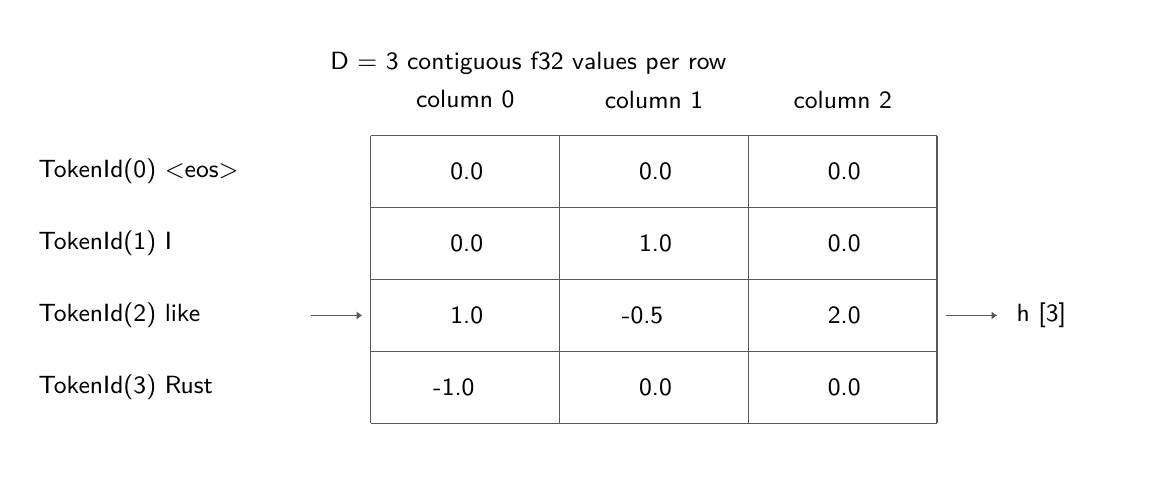
\begin{tikzpicture}[x=6.2pt,y=-13pt,draw=black!65,line width=.45pt]
\path[use as bounding box] (-1,-1) rectangle (63,11);
\node[anchor=west,inner sep=0pt,font=\sffamily\fontsize{9}{11}\selectfont] at (16.6,0) {\begin{adjustbox}{max width=217.0pt}D = 3 contiguous f32 values per row\end{adjustbox}};
\node[anchor=west,inner sep=0pt,font=\sffamily\fontsize{9}{11}\selectfont] at (21.6,1) {\begin{adjustbox}{max width=49.6pt}column 0\end{adjustbox}};
\node[anchor=west,inner sep=0pt,font=\sffamily\fontsize{9}{11}\selectfont] at (32.6,1) {\begin{adjustbox}{max width=49.6pt}column 1\end{adjustbox}};
\node[anchor=west,inner sep=0pt,font=\sffamily\fontsize{9}{11}\selectfont] at (43.6,1) {\begin{adjustbox}{max width=49.6pt}column 2\end{adjustbox}};
\draw (19,2) -- (19.5,2);
\draw (19,2) -- (19,2.5);
\draw (20,2) -- (19.5,2);
\draw (20,2) -- (20.5,2);
\draw (21,2) -- (20.5,2);
\draw (21,2) -- (21.5,2);
\draw (22,2) -- (21.5,2);
\draw (22,2) -- (22.5,2);
\draw (23,2) -- (22.5,2);
\draw (23,2) -- (23.5,2);
\draw (24,2) -- (23.5,2);
\draw (24,2) -- (24.5,2);
\draw (25,2) -- (24.5,2);
\draw (25,2) -- (25.5,2);
\draw (26,2) -- (25.5,2);
\draw (26,2) -- (26.5,2);
\draw (27,2) -- (26.5,2);
\draw (27,2) -- (27.5,2);
\draw (28,2) -- (27.5,2);
\draw (28,2) -- (28.5,2);
\draw (29,2) -- (28.5,2);
\draw (29,2) -- (29.5,2);
\draw (30,2) -- (29.5,2);
\draw (30,2) -- (30.5,2);
\draw (30,2) -- (30,2.5);
\draw (31,2) -- (30.5,2);
\draw (31,2) -- (31.5,2);
\draw (32,2) -- (31.5,2);
\draw (32,2) -- (32.5,2);
\draw (33,2) -- (32.5,2);
\draw (33,2) -- (33.5,2);
\draw (34,2) -- (33.5,2);
\draw (34,2) -- (34.5,2);
\draw (35,2) -- (34.5,2);
\draw (35,2) -- (35.5,2);
\draw (36,2) -- (35.5,2);
\draw (36,2) -- (36.5,2);
\draw (37,2) -- (36.5,2);
\draw (37,2) -- (37.5,2);
\draw (38,2) -- (37.5,2);
\draw (38,2) -- (38.5,2);
\draw (39,2) -- (38.5,2);
\draw (39,2) -- (39.5,2);
\draw (40,2) -- (39.5,2);
\draw (40,2) -- (40.5,2);
\draw (41,2) -- (40.5,2);
\draw (41,2) -- (41.5,2);
\draw (41,2) -- (41,2.5);
\draw (42,2) -- (41.5,2);
\draw (42,2) -- (42.5,2);
\draw (43,2) -- (42.5,2);
\draw (43,2) -- (43.5,2);
\draw (44,2) -- (43.5,2);
\draw (44,2) -- (44.5,2);
\draw (45,2) -- (44.5,2);
\draw (45,2) -- (45.5,2);
\draw (46,2) -- (45.5,2);
\draw (46,2) -- (46.5,2);
\draw (47,2) -- (46.5,2);
\draw (47,2) -- (47.5,2);
\draw (48,2) -- (47.5,2);
\draw (48,2) -- (48.5,2);
\draw (49,2) -- (48.5,2);
\draw (49,2) -- (49.5,2);
\draw (50,2) -- (49.5,2);
\draw (50,2) -- (50.5,2);
\draw (51,2) -- (50.5,2);
\draw (51,2) -- (51.5,2);
\draw (52,2) -- (51.5,2);
\draw (52,2) -- (52,2.5);
\draw (19,3) -- (19,2.5);
\draw (19,3) -- (19,3.5);
\draw (30,3) -- (30,2.5);
\draw (30,3) -- (30,3.5);
\draw (41,3) -- (41,2.5);
\draw (41,3) -- (41,3.5);
\draw (52,3) -- (52,2.5);
\draw (52,3) -- (52,3.5);
\node[anchor=west,inner sep=0pt,font=\sffamily\fontsize{9}{11}\selectfont] at (-0.4,3) {\begin{adjustbox}{max width=99.2pt}TokenId(0) <eos>\end{adjustbox}};
\node[anchor=west,inner sep=0pt,font=\sffamily\fontsize{9}{11}\selectfont] at (23.6,3) {\begin{adjustbox}{max width=18.6pt}0.0\end{adjustbox}};
\node[anchor=west,inner sep=0pt,font=\sffamily\fontsize{9}{11}\selectfont] at (34.6,3) {\begin{adjustbox}{max width=18.6pt}0.0\end{adjustbox}};
\node[anchor=west,inner sep=0pt,font=\sffamily\fontsize{9}{11}\selectfont] at (45.6,3) {\begin{adjustbox}{max width=18.6pt}0.0\end{adjustbox}};
\draw (19,4) -- (19,3.5);
\draw (19,4) -- (19.5,4);
\draw (19,4) -- (19,4.5);
\draw (20,4) -- (19.5,4);
\draw (20,4) -- (20.5,4);
\draw (21,4) -- (20.5,4);
\draw (21,4) -- (21.5,4);
\draw (22,4) -- (21.5,4);
\draw (22,4) -- (22.5,4);
\draw (23,4) -- (22.5,4);
\draw (23,4) -- (23.5,4);
\draw (24,4) -- (23.5,4);
\draw (24,4) -- (24.5,4);
\draw (25,4) -- (24.5,4);
\draw (25,4) -- (25.5,4);
\draw (26,4) -- (25.5,4);
\draw (26,4) -- (26.5,4);
\draw (27,4) -- (26.5,4);
\draw (27,4) -- (27.5,4);
\draw (28,4) -- (27.5,4);
\draw (28,4) -- (28.5,4);
\draw (29,4) -- (28.5,4);
\draw (29,4) -- (29.5,4);
\draw (30,4) -- (29.5,4);
\draw (30,4) -- (30.5,4);
\draw (30,4) -- (30,3.5);
\draw (30,4) -- (30,4.5);
\draw (31,4) -- (30.5,4);
\draw (31,4) -- (31.5,4);
\draw (32,4) -- (31.5,4);
\draw (32,4) -- (32.5,4);
\draw (33,4) -- (32.5,4);
\draw (33,4) -- (33.5,4);
\draw (34,4) -- (33.5,4);
\draw (34,4) -- (34.5,4);
\draw (35,4) -- (34.5,4);
\draw (35,4) -- (35.5,4);
\draw (36,4) -- (35.5,4);
\draw (36,4) -- (36.5,4);
\draw (37,4) -- (36.5,4);
\draw (37,4) -- (37.5,4);
\draw (38,4) -- (37.5,4);
\draw (38,4) -- (38.5,4);
\draw (39,4) -- (38.5,4);
\draw (39,4) -- (39.5,4);
\draw (40,4) -- (39.5,4);
\draw (40,4) -- (40.5,4);
\draw (41,4) -- (40.5,4);
\draw (41,4) -- (41.5,4);
\draw (41,4) -- (41,3.5);
\draw (41,4) -- (41,4.5);
\draw (42,4) -- (41.5,4);
\draw (42,4) -- (42.5,4);
\draw (43,4) -- (42.5,4);
\draw (43,4) -- (43.5,4);
\draw (44,4) -- (43.5,4);
\draw (44,4) -- (44.5,4);
\draw (45,4) -- (44.5,4);
\draw (45,4) -- (45.5,4);
\draw (46,4) -- (45.5,4);
\draw (46,4) -- (46.5,4);
\draw (47,4) -- (46.5,4);
\draw (47,4) -- (47.5,4);
\draw (48,4) -- (47.5,4);
\draw (48,4) -- (48.5,4);
\draw (49,4) -- (48.5,4);
\draw (49,4) -- (49.5,4);
\draw (50,4) -- (49.5,4);
\draw (50,4) -- (50.5,4);
\draw (51,4) -- (50.5,4);
\draw (51,4) -- (51.5,4);
\draw (52,4) -- (52,3.5);
\draw (52,4) -- (51.5,4);
\draw (52,4) -- (52,4.5);
\draw (19,5) -- (19,4.5);
\draw (19,5) -- (19,5.5);
\draw (30,5) -- (30,4.5);
\draw (30,5) -- (30,5.5);
\draw (41,5) -- (41,4.5);
\draw (41,5) -- (41,5.5);
\draw (52,5) -- (52,4.5);
\draw (52,5) -- (52,5.5);
\node[anchor=west,inner sep=0pt,font=\sffamily\fontsize{9}{11}\selectfont] at (-0.4,5) {\begin{adjustbox}{max width=74.4pt}TokenId(1) I\end{adjustbox}};
\node[anchor=west,inner sep=0pt,font=\sffamily\fontsize{9}{11}\selectfont] at (23.6,5) {\begin{adjustbox}{max width=18.6pt}0.0\end{adjustbox}};
\node[anchor=west,inner sep=0pt,font=\sffamily\fontsize{9}{11}\selectfont] at (34.6,5) {\begin{adjustbox}{max width=18.6pt}1.0\end{adjustbox}};
\node[anchor=west,inner sep=0pt,font=\sffamily\fontsize{9}{11}\selectfont] at (45.6,5) {\begin{adjustbox}{max width=18.6pt}0.0\end{adjustbox}};
\draw (19,6) -- (19,5.5);
\draw (19,6) -- (19.5,6);
\draw (19,6) -- (19,6.5);
\draw (20,6) -- (19.5,6);
\draw (20,6) -- (20.5,6);
\draw (21,6) -- (20.5,6);
\draw (21,6) -- (21.5,6);
\draw (22,6) -- (21.5,6);
\draw (22,6) -- (22.5,6);
\draw (23,6) -- (22.5,6);
\draw (23,6) -- (23.5,6);
\draw (24,6) -- (23.5,6);
\draw (24,6) -- (24.5,6);
\draw (25,6) -- (24.5,6);
\draw (25,6) -- (25.5,6);
\draw (26,6) -- (25.5,6);
\draw (26,6) -- (26.5,6);
\draw (27,6) -- (26.5,6);
\draw (27,6) -- (27.5,6);
\draw (28,6) -- (27.5,6);
\draw (28,6) -- (28.5,6);
\draw (29,6) -- (28.5,6);
\draw (29,6) -- (29.5,6);
\draw (30,6) -- (29.5,6);
\draw (30,6) -- (30.5,6);
\draw (30,6) -- (30,5.5);
\draw (30,6) -- (30,6.5);
\draw (31,6) -- (30.5,6);
\draw (31,6) -- (31.5,6);
\draw (32,6) -- (31.5,6);
\draw (32,6) -- (32.5,6);
\draw (33,6) -- (32.5,6);
\draw (33,6) -- (33.5,6);
\draw (34,6) -- (33.5,6);
\draw (34,6) -- (34.5,6);
\draw (35,6) -- (34.5,6);
\draw (35,6) -- (35.5,6);
\draw (36,6) -- (35.5,6);
\draw (36,6) -- (36.5,6);
\draw (37,6) -- (36.5,6);
\draw (37,6) -- (37.5,6);
\draw (38,6) -- (37.5,6);
\draw (38,6) -- (38.5,6);
\draw (39,6) -- (38.5,6);
\draw (39,6) -- (39.5,6);
\draw (40,6) -- (39.5,6);
\draw (40,6) -- (40.5,6);
\draw (41,6) -- (40.5,6);
\draw (41,6) -- (41.5,6);
\draw (41,6) -- (41,5.5);
\draw (41,6) -- (41,6.5);
\draw (42,6) -- (41.5,6);
\draw (42,6) -- (42.5,6);
\draw (43,6) -- (42.5,6);
\draw (43,6) -- (43.5,6);
\draw (44,6) -- (43.5,6);
\draw (44,6) -- (44.5,6);
\draw (45,6) -- (44.5,6);
\draw (45,6) -- (45.5,6);
\draw (46,6) -- (45.5,6);
\draw (46,6) -- (46.5,6);
\draw (47,6) -- (46.5,6);
\draw (47,6) -- (47.5,6);
\draw (48,6) -- (47.5,6);
\draw (48,6) -- (48.5,6);
\draw (49,6) -- (48.5,6);
\draw (49,6) -- (49.5,6);
\draw (50,6) -- (49.5,6);
\draw (50,6) -- (50.5,6);
\draw (51,6) -- (50.5,6);
\draw (51,6) -- (51.5,6);
\draw (52,6) -- (52,5.5);
\draw (52,6) -- (51.5,6);
\draw (52,6) -- (52,6.5);
\draw (16,7) -- (15.5,7);
\draw (16,7) -- (16.5,7);
\draw (17,7) -- (16.5,7);
\draw (17,7) -- (17.5,7);
\draw[-{Latex[length=2pt,width=3pt]}] (17.5,7) -- (18.5,7);
\draw (19,7) -- (19,6.5);
\draw (19,7) -- (19,7.5);
\draw (30,7) -- (30,6.5);
\draw (30,7) -- (30,7.5);
\draw (41,7) -- (41,6.5);
\draw (41,7) -- (41,7.5);
\draw (52,7) -- (52,6.5);
\draw (52,7) -- (52,7.5);
\draw (53,7) -- (52.5,7);
\draw (53,7) -- (53.5,7);
\draw (54,7) -- (53.5,7);
\draw (54,7) -- (54.5,7);
\draw[-{Latex[length=2pt,width=3pt]}] (54.5,7) -- (55.5,7);
\node[anchor=west,inner sep=0pt,font=\sffamily\fontsize{9}{11}\selectfont] at (-0.4,7) {\begin{adjustbox}{max width=93.0pt}TokenId(2) like\end{adjustbox}};
\node[anchor=west,inner sep=0pt,font=\sffamily\fontsize{9}{11}\selectfont] at (23.6,7) {\begin{adjustbox}{max width=18.6pt}1.0\end{adjustbox}};
\node[anchor=west,inner sep=0pt,font=\sffamily\fontsize{9}{11}\selectfont] at (33.6,7) {\begin{adjustbox}{max width=24.8pt}-0.5\end{adjustbox}};
\node[anchor=west,inner sep=0pt,font=\sffamily\fontsize{9}{11}\selectfont] at (45.6,7) {\begin{adjustbox}{max width=18.6pt}2.0\end{adjustbox}};
\node[anchor=west,inner sep=0pt,font=\sffamily\fontsize{9}{11}\selectfont] at (56.6,7) {\begin{adjustbox}{max width=31.0pt}h [3]\end{adjustbox}};
\draw (19,8) -- (19,7.5);
\draw (19,8) -- (19.5,8);
\draw (19,8) -- (19,8.5);
\draw (20,8) -- (19.5,8);
\draw (20,8) -- (20.5,8);
\draw (21,8) -- (20.5,8);
\draw (21,8) -- (21.5,8);
\draw (22,8) -- (21.5,8);
\draw (22,8) -- (22.5,8);
\draw (23,8) -- (22.5,8);
\draw (23,8) -- (23.5,8);
\draw (24,8) -- (23.5,8);
\draw (24,8) -- (24.5,8);
\draw (25,8) -- (24.5,8);
\draw (25,8) -- (25.5,8);
\draw (26,8) -- (25.5,8);
\draw (26,8) -- (26.5,8);
\draw (27,8) -- (26.5,8);
\draw (27,8) -- (27.5,8);
\draw (28,8) -- (27.5,8);
\draw (28,8) -- (28.5,8);
\draw (29,8) -- (28.5,8);
\draw (29,8) -- (29.5,8);
\draw (30,8) -- (29.5,8);
\draw (30,8) -- (30.5,8);
\draw (30,8) -- (30,7.5);
\draw (30,8) -- (30,8.5);
\draw (31,8) -- (30.5,8);
\draw (31,8) -- (31.5,8);
\draw (32,8) -- (31.5,8);
\draw (32,8) -- (32.5,8);
\draw (33,8) -- (32.5,8);
\draw (33,8) -- (33.5,8);
\draw (34,8) -- (33.5,8);
\draw (34,8) -- (34.5,8);
\draw (35,8) -- (34.5,8);
\draw (35,8) -- (35.5,8);
\draw (36,8) -- (35.5,8);
\draw (36,8) -- (36.5,8);
\draw (37,8) -- (36.5,8);
\draw (37,8) -- (37.5,8);
\draw (38,8) -- (37.5,8);
\draw (38,8) -- (38.5,8);
\draw (39,8) -- (38.5,8);
\draw (39,8) -- (39.5,8);
\draw (40,8) -- (39.5,8);
\draw (40,8) -- (40.5,8);
\draw (41,8) -- (40.5,8);
\draw (41,8) -- (41.5,8);
\draw (41,8) -- (41,7.5);
\draw (41,8) -- (41,8.5);
\draw (42,8) -- (41.5,8);
\draw (42,8) -- (42.5,8);
\draw (43,8) -- (42.5,8);
\draw (43,8) -- (43.5,8);
\draw (44,8) -- (43.5,8);
\draw (44,8) -- (44.5,8);
\draw (45,8) -- (44.5,8);
\draw (45,8) -- (45.5,8);
\draw (46,8) -- (45.5,8);
\draw (46,8) -- (46.5,8);
\draw (47,8) -- (46.5,8);
\draw (47,8) -- (47.5,8);
\draw (48,8) -- (47.5,8);
\draw (48,8) -- (48.5,8);
\draw (49,8) -- (48.5,8);
\draw (49,8) -- (49.5,8);
\draw (50,8) -- (49.5,8);
\draw (50,8) -- (50.5,8);
\draw (51,8) -- (50.5,8);
\draw (51,8) -- (51.5,8);
\draw (52,8) -- (52,7.5);
\draw (52,8) -- (51.5,8);
\draw (52,8) -- (52,8.5);
\draw (19,9) -- (19,8.5);
\draw (19,9) -- (19,9.5);
\draw (30,9) -- (30,8.5);
\draw (30,9) -- (30,9.5);
\draw (41,9) -- (41,8.5);
\draw (41,9) -- (41,9.5);
\draw (52,9) -- (52,8.5);
\draw (52,9) -- (52,9.5);
\node[anchor=west,inner sep=0pt,font=\sffamily\fontsize{9}{11}\selectfont] at (-0.4,9) {\begin{adjustbox}{max width=93.0pt}TokenId(3) Rust\end{adjustbox}};
\node[anchor=west,inner sep=0pt,font=\sffamily\fontsize{9}{11}\selectfont] at (22.6,9) {\begin{adjustbox}{max width=24.8pt}-1.0\end{adjustbox}};
\node[anchor=west,inner sep=0pt,font=\sffamily\fontsize{9}{11}\selectfont] at (34.6,9) {\begin{adjustbox}{max width=18.6pt}0.0\end{adjustbox}};
\node[anchor=west,inner sep=0pt,font=\sffamily\fontsize{9}{11}\selectfont] at (45.6,9) {\begin{adjustbox}{max width=18.6pt}0.0\end{adjustbox}};
\draw (19,10) -- (19.5,10);
\draw (19,10) -- (19,9.5);
\draw (20,10) -- (19.5,10);
\draw (20,10) -- (20.5,10);
\draw (21,10) -- (20.5,10);
\draw (21,10) -- (21.5,10);
\draw (22,10) -- (21.5,10);
\draw (22,10) -- (22.5,10);
\draw (23,10) -- (22.5,10);
\draw (23,10) -- (23.5,10);
\draw (24,10) -- (23.5,10);
\draw (24,10) -- (24.5,10);
\draw (25,10) -- (24.5,10);
\draw (25,10) -- (25.5,10);
\draw (26,10) -- (25.5,10);
\draw (26,10) -- (26.5,10);
\draw (27,10) -- (26.5,10);
\draw (27,10) -- (27.5,10);
\draw (28,10) -- (27.5,10);
\draw (28,10) -- (28.5,10);
\draw (29,10) -- (28.5,10);
\draw (29,10) -- (29.5,10);
\draw (30,10) -- (29.5,10);
\draw (30,10) -- (30.5,10);
\draw (30,10) -- (30,9.5);
\draw (31,10) -- (30.5,10);
\draw (31,10) -- (31.5,10);
\draw (32,10) -- (31.5,10);
\draw (32,10) -- (32.5,10);
\draw (33,10) -- (32.5,10);
\draw (33,10) -- (33.5,10);
\draw (34,10) -- (33.5,10);
\draw (34,10) -- (34.5,10);
\draw (35,10) -- (34.5,10);
\draw (35,10) -- (35.5,10);
\draw (36,10) -- (35.5,10);
\draw (36,10) -- (36.5,10);
\draw (37,10) -- (36.5,10);
\draw (37,10) -- (37.5,10);
\draw (38,10) -- (37.5,10);
\draw (38,10) -- (38.5,10);
\draw (39,10) -- (38.5,10);
\draw (39,10) -- (39.5,10);
\draw (40,10) -- (39.5,10);
\draw (40,10) -- (40.5,10);
\draw (41,10) -- (40.5,10);
\draw (41,10) -- (41.5,10);
\draw (41,10) -- (41,9.5);
\draw (42,10) -- (41.5,10);
\draw (42,10) -- (42.5,10);
\draw (43,10) -- (42.5,10);
\draw (43,10) -- (43.5,10);
\draw (44,10) -- (43.5,10);
\draw (44,10) -- (44.5,10);
\draw (45,10) -- (44.5,10);
\draw (45,10) -- (45.5,10);
\draw (46,10) -- (45.5,10);
\draw (46,10) -- (46.5,10);
\draw (47,10) -- (46.5,10);
\draw (47,10) -- (47.5,10);
\draw (48,10) -- (47.5,10);
\draw (48,10) -- (48.5,10);
\draw (49,10) -- (48.5,10);
\draw (49,10) -- (49.5,10);
\draw (50,10) -- (49.5,10);
\draw (50,10) -- (50.5,10);
\draw (51,10) -- (50.5,10);
\draw (51,10) -- (51.5,10);
\draw (52,10) -- (51.5,10);
\draw (52,10) -- (52,9.5);
\end{tikzpicture}
\end{adjustbox}\end{center}

For \(x=2\), the result is

\[
\mathbf{h}=[1.0,-0.5,2.0].
\]

This is a row selection, sometimes called a gather. ENGINE-1 computes
the row start at the element offset

\[
o_{\mathrm{row}}=xD\quad[\mathrm{elements}].
\]

and copies the next \texttt{D} values. The scalar value 2 is used only
in address calculation. We do not multiply the vector by 2.

\subsubsection{Why not feed the integer directly into
arithmetic?}\label{why-not-feed-the-integer-directly-into-arithmetic}

Imagine that vocabulary revision A assigns:

\begin{verbatim}
2 -> like
3 -> Rust
\end{verbatim}

and revision B assigns:

\begin{verbatim}
2 -> Rust
3 -> like
\end{verbatim}

The language meanings swapped while the integers did not. Any rule that
treats 3 as inherently larger or closer to something than 2 would change
meaning when the vocabulary was renumbered. Embedding rows attach
numerical parameters to identities explicitly.

An embedding does not guarantee that each dimension has a clean human
label. We must not say that dimension 0 is ``programming,'' dimension 1
is ``affection,'' or dimension 2 is ``grammar'' merely because a tiny
hand fixture makes a story tempting. In a trained model, useful behavior
can be distributed across many dimensions. For ENGINE-1, \texttt{h} is
exactly this: the numerical representation of the current input token
consumed by the next computation.

\subsubsection{Is lookup secretly matrix
multiplication?}\label{is-lookup-secretly-matrix-multiplication}

We could represent token 2 as a one-hot vector:

\begin{verbatim}
[0, 0, 1, 0]
\end{verbatim}

and multiply it by \texttt{E}. The result would select row 2. That
equivalence can be useful mathematically, but it is a poor description
of ENGINE-1's execution. Materializing \texttt{V} values, almost all
zero, and multiplying through every row would hide the actual access
pattern. The code reads one contiguous row.

\begin{quote}
\textbf{FIRST PRINCIPLE} An embedding lookup reads the row named by a
token ID. It does not assign meaning to the ID's integer magnitude, and
it need not execute as dense matrix multiplication.
\end{quote}

\subsection{One score for every possible next
token}\label{one-score-for-every-possible-next-token}

The hidden vector represents the input. The model now needs one score
for each candidate next token. The result has \(V_{\mathrm{vocab}}\)
components.

Introduce an \textbf{output projection} matrix \(\mathbf{W}\) and bias
vector \(\mathbf{b}\):

\[
\mathbf{W}\in\mathbb{R}^{V_{\mathrm{vocab}}\times D},
\qquad \mathbf{b}\in\mathbb{R}^{V_{\mathrm{vocab}}}.
\]

Each row \(\mathbf{W}_{i,:}\) belongs to candidate token \(i\). Compute

\[
\mathbf{z}=\mathbf{W}\mathbf{h}+\mathbf{b},
\qquad \mathbf{z}\in\mathbb{R}^{V_{\mathrm{vocab}}}.
\]

For one candidate \(i\):

\[
z_i=b_i+\sum_{j=0}^{D-1}W_{ij}h_j,
\qquad 0\le i<V_{\mathrm{vocab}}.
\]

This operation takes the \textbf{dot product} of row \texttt{i} and
\texttt{h}, then adds one bias. The
\href{https://github.com/hermonai/inside-the-llm-engine/blob/astra-visual-rewrite/diagrams/model/one-logit-dot-product.txt}{one-logit
diagram} connects vector notation to scalar arithmetic:

\begin{center}\begin{adjustbox}{max width=\linewidth}% Legacy topology preserved as native vectors and typeset labels.
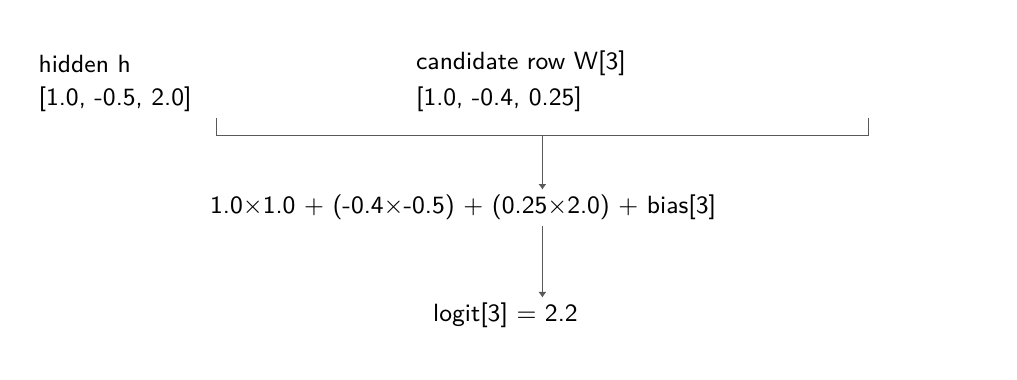
\begin{tikzpicture}[x=6.2pt,y=-13pt,draw=black!65,line width=.45pt]
\path[use as bounding box] (-1,-1) rectangle (55,8);
\node[anchor=west,inner sep=0pt,font=\sffamily\fontsize{9}{11}\selectfont] at (-0.4,0) {\begin{adjustbox}{max width=49.6pt}hidden h\end{adjustbox}};
\node[anchor=west,inner sep=0pt,font=\sffamily\fontsize{9}{11}\selectfont] at (21.6,0) {\begin{adjustbox}{max width=111.60000000000001pt}candidate row W[3]\end{adjustbox}};
\node[anchor=west,inner sep=0pt,font=\sffamily\fontsize{9}{11}\selectfont] at (-0.4,1) {\begin{adjustbox}{max width=99.2pt}[1.0, -0.5, 2.0]\end{adjustbox}};
\node[anchor=west,inner sep=0pt,font=\sffamily\fontsize{9}{11}\selectfont] at (21.6,1) {\begin{adjustbox}{max width=105.4pt}[1.0, -0.4, 0.25]\end{adjustbox}};
\draw (10,2) -- (10.5,2);
\draw (10,2) -- (10,1.5);
\draw (11,2) -- (10.5,2);
\draw (11,2) -- (11.5,2);
\draw (12,2) -- (11.5,2);
\draw (12,2) -- (12.5,2);
\draw (13,2) -- (12.5,2);
\draw (13,2) -- (13.5,2);
\draw (14,2) -- (13.5,2);
\draw (14,2) -- (14.5,2);
\draw (15,2) -- (14.5,2);
\draw (15,2) -- (15.5,2);
\draw (16,2) -- (15.5,2);
\draw (16,2) -- (16.5,2);
\draw (17,2) -- (16.5,2);
\draw (17,2) -- (17.5,2);
\draw (18,2) -- (17.5,2);
\draw (18,2) -- (18.5,2);
\draw (19,2) -- (18.5,2);
\draw (19,2) -- (19.5,2);
\draw (20,2) -- (19.5,2);
\draw (20,2) -- (20.5,2);
\draw (21,2) -- (20.5,2);
\draw (21,2) -- (21.5,2);
\draw (22,2) -- (21.5,2);
\draw (22,2) -- (22.5,2);
\draw (23,2) -- (22.5,2);
\draw (23,2) -- (23.5,2);
\draw (24,2) -- (23.5,2);
\draw (24,2) -- (24.5,2);
\draw (25,2) -- (24.5,2);
\draw (25,2) -- (25.5,2);
\draw (26,2) -- (25.5,2);
\draw (26,2) -- (26.5,2);
\draw (27,2) -- (26.5,2);
\draw (27,2) -- (27.5,2);
\draw (28,2) -- (27.5,2);
\draw (28,2) -- (28.5,2);
\draw (29,2) -- (28.5,2);
\draw (29,2) -- (29.5,2);
\draw (29,2) -- (29,2.5);
\draw (30,2) -- (29.5,2);
\draw (30,2) -- (30.5,2);
\draw (31,2) -- (30.5,2);
\draw (31,2) -- (31.5,2);
\draw (32,2) -- (31.5,2);
\draw (32,2) -- (32.5,2);
\draw (33,2) -- (32.5,2);
\draw (33,2) -- (33.5,2);
\draw (34,2) -- (33.5,2);
\draw (34,2) -- (34.5,2);
\draw (35,2) -- (34.5,2);
\draw (35,2) -- (35.5,2);
\draw (36,2) -- (35.5,2);
\draw (36,2) -- (36.5,2);
\draw (37,2) -- (36.5,2);
\draw (37,2) -- (37.5,2);
\draw (38,2) -- (37.5,2);
\draw (38,2) -- (38.5,2);
\draw (39,2) -- (38.5,2);
\draw (39,2) -- (39.5,2);
\draw (40,2) -- (39.5,2);
\draw (40,2) -- (40.5,2);
\draw (41,2) -- (40.5,2);
\draw (41,2) -- (41.5,2);
\draw (42,2) -- (41.5,2);
\draw (42,2) -- (42.5,2);
\draw (43,2) -- (42.5,2);
\draw (43,2) -- (43.5,2);
\draw (44,2) -- (43.5,2);
\draw (44,2) -- (44.5,2);
\draw (45,2) -- (44.5,2);
\draw (45,2) -- (45.5,2);
\draw (46,2) -- (45.5,2);
\draw (46,2) -- (46.5,2);
\draw (47,2) -- (46.5,2);
\draw (47,2) -- (47.5,2);
\draw (48,2) -- (47.5,2);
\draw (48,2) -- (48,1.5);
\draw[-{Latex[length=2pt,width=3pt]}] (29,2.5) -- (29,3.5);
\node[anchor=west,inner sep=0pt,font=\sffamily\fontsize{9}{11}\selectfont] at (9.6,4) {\begin{adjustbox}{max width=272.8pt}1.0×1.0 + (-0.4×-0.5) + (0.25×2.0) + bias[3]\end{adjustbox}};
\draw (29,5) -- (29,4.5);
\draw (29,5) -- (29,5.5);
\draw[-{Latex[length=2pt,width=3pt]}] (29,5.5) -- (29,6.5);
\node[anchor=west,inner sep=0pt,font=\sffamily\fontsize{9}{11}\selectfont] at (22.6,7) {\begin{adjustbox}{max width=86.8pt}logit[3] = 2.2\end{adjustbox}};
\end{tikzpicture}
\end{adjustbox}\end{center}

Repeat that operation for all \(V_{\mathrm{vocab}}\) rows. Matrix
notation compresses the idea; the implementation exposes the work:

\begin{verbatim}
for output in 0..vocab_size {
    let mut accumulator = output_bias[output];
    let row_start = output * hidden_dim;
    for dimension in 0..hidden_dim {
        accumulator +=
            output_weight[row_start + dimension] * hidden[dimension];
    }
    logits[output] = accumulator;
}
\end{verbatim}

The inner loop calculates one candidate score. The outer loop repeats it
for the vocabulary. There is no answer table in this code: changing an
embedding, projection weight, or bias changes the arithmetic that
produces the vector. The canonical
\href{https://github.com/hermonai/inside-the-llm-engine/blob/astra-visual-rewrite/diagrams/model/engine-1-overview.txt}{ENGINE-1
overview} places those immutable parameters beside request-owned history
and sampler state.

\subsubsection{``Linear'' layers usually include
bias}\label{linear-layers-usually-include-bias}

Strictly, \texttt{W\ h} is a linear map and \texttt{W\ h\ +\ b} is
affine when \texttt{b} is nonzero. Machine-learning libraries commonly
call the combined operation a linear layer. We will use \textbf{output
projection} for the role and write the bias explicitly so neither
terminology nor code can hide it.

\subsection{What a logit is---and is
not}\label{what-a-logit-isand-is-not}

Each \texttt{z\_i} is a \textbf{logit}: an unnormalized numerical score
for candidate token \texttt{i}. ENGINE-1's complete result for
\texttt{like} will be:

\begin{verbatim}
token       logit
<eos>       -0.7
I            0.1
like         0.4
Rust         2.2
\end{verbatim}

The values do not sum to 1. They can be negative. A logit of 2.2 is not
a probability of 2.2, 220 percent, or ``2.2 times likely.'' A difference
of 1.8 is not directly a probability difference. We have not yet defined
the transformation needed for those interpretations.

For a deterministic argmax policy, the larger finite score wins, so
\texttt{Rust} would be selected here. That statement is about ordering
only. It does not make the largest score probability 1, and it does not
make argmax part of the model.

The boundary remains:

\begin{verbatim}
Model::forward(history) -> Logits
Selector::select(logits) -> TokenId
\end{verbatim}

ENGINE-0 blurred this distinction because the fake model returned
candidates already carrying token kinds and integer scores. ENGINE-1
returns a typed \texttt{Logits} vector. The selector scans it. The
runtime uses the model/tokenizer contract to recognize EOS and otherwise
asks the tokenizer for output bytes.

\begin{quote}
\textbf{FIRST PRINCIPLE} The model produces logits. Token selection is a
separate engine policy.
\end{quote}

Chapter 4 owns softmax, numerical stability, temperature, randomness,
seeds, top-k, top-p, and the complete feedback loop. We will not smuggle
those topics into \texttt{forward} merely to make this chapter appear
more complete.

\subsection{The complete hand-calculated forward
pass}\label{the-complete-hand-calculated-forward-pass}

Our vocabulary has four identities:

\begin{verbatim}
0 <eos>
1 I
2 like
3 Rust
\end{verbatim}

The hidden dimension is three. Therefore \(V_{\mathrm{vocab}}=4\) and
\(D=3\). The parameters are:

\begin{verbatim}
E = [
  [ 0.0,  0.0,  0.0],
  [ 0.0,  1.0,  0.0],
  [ 1.0, -0.5,  2.0],
  [-1.0,  0.0,  0.0],
]

W = [
  [-0.5,  0.4,  0.1],
  [ 0.2,  0.2,  0.0],
  [ 0.3,  0.2,  0.1],
  [ 1.0, -0.4,  0.25],
]

b = [-0.2, 0.0, 0.0, 0.5]
\end{verbatim}

These values are supplied directly. In a real neural language model,
training would normally produce parameters by optimizing an objective
over data. This book is about inference, so we hold training outside the
boundary. ``Learned parameters'' names their usual origin; it does not
mean ENGINE-1 trains them.

Input \texttt{like} has ID 2. First select the embedding row:

\[
\mathbf{h}=\mathbf{E}_{2,:}=[1.0,-0.5,2.0].
\]

Now calculate every candidate.

All four candidate rows follow the same contract:

\[
\begin{aligned}
z_0&=-0.2+(-0.5)(1.0)+(0.4)(-0.5)+(0.1)(2.0)=-0.7,\\
z_1&= 0.0+(0.2)(1.0)+(0.2)(-0.5)+(0.0)(2.0)= 0.1,\\
z_2&= 0.0+(0.3)(1.0)+(0.2)(-0.5)+(0.1)(2.0)= 0.4,\\
z_3&= 0.5+(1.0)(1.0)+(-0.4)(-0.5)+(0.25)(2.0)=2.2.
\end{aligned}
\]

Therefore the full oracle is

\[
\mathbf{z}=[-0.7,0.1,0.4,2.2].
\]

Notice what the oracle does not say. It does not say merely ``the answer
is token 3.'' Many wrong vectors can share the same largest index. A
transposed matrix, missing bias, wrong embedding row, or misaligned
vocabulary can still produce argmax 3 by accident.

\begin{quote}
\textbf{FIRST PRINCIPLE} A correct selected token does not prove that
the model produced correct logits.
\end{quote}

\subsection{An independent numerical
oracle}\label{an-independent-numerical-oracle}

The Rust model and its test could share the same indexing bug. Rewriting
the same function under a different name would not provide much
independence. The repository therefore includes a plain-Python oracle in
\texttt{\seqsplit{code/reference/python/chapter03\_oracle.py}}.

The script defines \texttt{E}, \texttt{W}, and \texttt{b} separately,
selects the row, implements the equations with its own loops, and
asserts the full expected vector. It does not import ENGINE-1, call the
Rust binary, or use NumPy. Run it with:

\begin{verbatim}
python3 code/reference/python/chapter03_oracle.py
\end{verbatim}

Expected output includes:

\begin{verbatim}
input=2:like
hidden=[1.0, -0.5, 2.0]
logits=[-0.7, 0.1, 0.4, 2.2]
oracle=PASS
\end{verbatim}

The Rust differential uses a small absolute-plus-relative tolerance:

\[
|a-r|\le \epsilon_{\mathrm{abs}}+
\epsilon_{\mathrm{rel}}|r|,
\]

Why not exact equality? Several fixture values happen to have exact
binary representations, and this short reduction is deterministic on the
current scalar path. But floating-point arithmetic generally rounds, and
later execution providers may change reduction order. An absolute
tolerance covers small values near zero; a relative tolerance scales
with larger expected values. The tolerance must be tight enough to catch
errors and documented instead of chosen after seeing a failure.

The model also rejects non-finite parameters and non-finite output
logits. \texttt{NaN} is especially dangerous because comparisons with it
are false; a naive argmax scan can silently keep an unrelated candidate.
Some future operations may deliberately use infinities to represent
masks. ENGINE-1 has no mask or logits processor, so \texttt{NaN},
positive infinity, and negative infinity indicate invalid numerical
state at this boundary.

\subsection{A tensor, before a tensor
framework}\label{a-tensor-before-a-tensor-framework}

Chapter 5 will treat tensors systematically. We need a smaller working
definition now. A \textbf{tensor} is numerical data interpreted with
metadata and contracts such as:

\begin{itemize}
\tightlist
\item
  shape;
\item
  element type, or \textbf{dtype};
\item
  physical data;
\item
  layout and strides;
\item
  owner and lifetime;
\item
  device or location.
\end{itemize}

ENGINE-1 uses only one location, the CPU, and one storage type,
\texttt{f32}. All arrays are contiguous. Matrices are row-major. There
is no dynamic rank, broadcasting, autograd, GPU abstraction, or general
stride machinery.

The canonical
\href{https://github.com/hermonai/inside-the-llm-engine/blob/astra-visual-rewrite/diagrams/model/tiny-model-tensor-shapes.txt}{shape
table} is:

{\def\LTcaptype{none} % do not increment counter
\begin{longtable}[]{@{}lllll@{}}
\toprule\noalign{}
Name & Symbol & Shape & Lifetime & Inference-mutable? \\
\midrule\noalign{}
\endhead
\bottomrule\noalign{}
\endlastfoot
Embedding & \texttt{E} & \texttt{{[}V,D{]}} & model & no \\
Projection & \texttt{W} & \texttt{{[}V,D{]}} & model & no \\
Bias & \texttt{b} & \texttt{{[}V{]}} & model & no \\
Input token & \texttt{x} & scalar & request/step & new \\
Hidden & \texttt{h} & \texttt{{[}D{]}} & forward & new \\
Logits & \texttt{z} & \texttt{{[}V{]}} & forward/result & new \\
\end{longtable}
}

``Mutable?'' in this table describes inference semantics. A loader may
fill an allocation during construction, and Rust's
\texttt{Vec\textless{}f32\textgreater{}} is mechanically capable of
mutation. After construction, ordinary forward inference does not change
parameters. \texttt{\seqsplit{TinyLanguageModel::forward}} takes
\texttt{\&self}, making that rule visible in the API.

\begin{quote}
\textbf{FIRST PRINCIPLE} Every tensor needs an explicit shape, dtype,
layout, owner, lifetime, and access pattern. Shape is an executable
contract, not decoration.
\end{quote}

\subsection{Logical shape and physical row-major
memory}\label{logical-shape-and-physical-row-major-memory}

\texttt{W} has logical shape \texttt{{[}V,D{]}}. For \texttt{V=4},
\texttt{D=3}, picture four rows and three columns:

\begin{verbatim}
W[0,0] W[0,1] W[0,2]
W[1,0] W[1,1] W[1,2]
W[2,0] W[2,1] W[2,2]
W[3,0] W[3,1] W[3,2]
\end{verbatim}

The contiguous physical vector is:

\begin{verbatim}
[W00, W01, W02, W10, W11, W12, W20, W21, W22, W30, W31, W32]
\end{verbatim}

The offset for logical element \texttt{(row,\ column)} is:

\begin{verbatim}
offset = row * D + column
\end{verbatim}

This convention is not forced by the equation. We could store columns
contiguously, pad rows, tile blocks, quantize groups, or use
provider-specific layouts. Those choices would change access and kernels
without changing the model's mathematical meaning. ENGINE-1 chooses
row-major because one output candidate consumes one complete row, so the
inner loop reads contiguous weights.

Matrix notation alone cannot tell us whether bytes are contiguous,
transposed, padded, packed, resident on a device, or available through a
view. An engine must connect logical indices to physical addresses.

\subsection{Parameters and activations are different
memory}\label{parameters-and-activations-are-different-memory}

The embedding, projection, and bias are \textbf{parameters}: persistent
values that define model behavior. The selected hidden row and logits
are \textbf{activations}: values produced while executing the model for
a particular input.

The
\href{https://github.com/hermonai/inside-the-llm-engine/blob/astra-visual-rewrite/diagrams/model/parameters-vs-activations.txt}{ownership
diagram} shows why the distinction matters:

\begin{center}\begin{adjustbox}{max width=\linewidth}% Legacy topology preserved as native vectors and typeset labels.
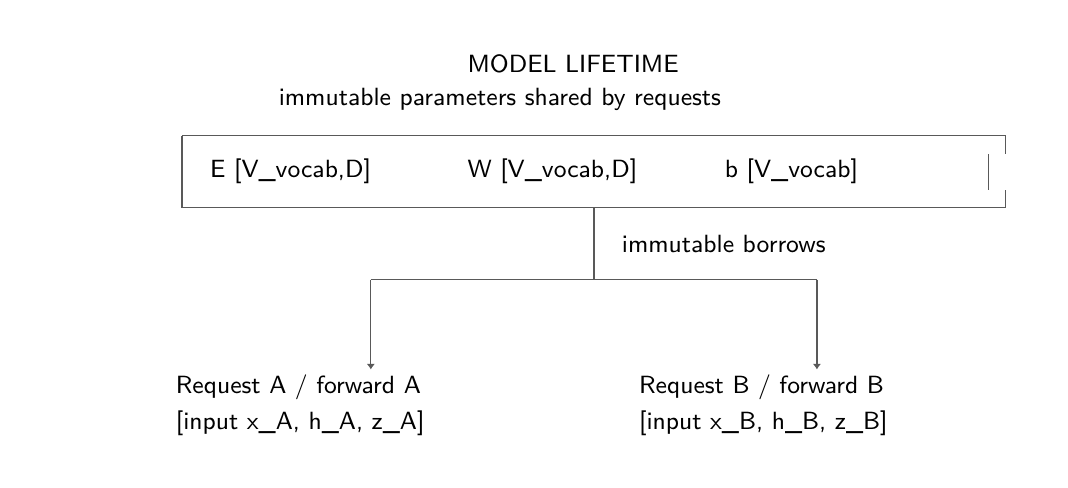
\begin{tikzpicture}[x=6.2pt,y=-13pt,draw=black!65,line width=.45pt]
\path[use as bounding box] (-1,-1) rectangle (58,11);
\node[anchor=west,inner sep=0pt,font=\sffamily\fontsize{9}{11}\selectfont] at (24.6,0) {\begin{adjustbox}{max width=86.8pt}MODEL LIFETIME\end{adjustbox}};
\node[anchor=west,inner sep=0pt,font=\sffamily\fontsize{9}{11}\selectfont] at (13.6,1) {\begin{adjustbox}{max width=241.8pt}immutable parameters shared by requests\end{adjustbox}};
\draw (8,2) -- (8.5,2);
\draw (8,2) -- (8,2.5);
\draw (9,2) -- (8.5,2);
\draw (9,2) -- (9.5,2);
\draw (10,2) -- (9.5,2);
\draw (10,2) -- (10.5,2);
\draw (11,2) -- (10.5,2);
\draw (11,2) -- (11.5,2);
\draw (12,2) -- (11.5,2);
\draw (12,2) -- (12.5,2);
\draw (13,2) -- (12.5,2);
\draw (13,2) -- (13.5,2);
\draw (14,2) -- (13.5,2);
\draw (14,2) -- (14.5,2);
\draw (15,2) -- (14.5,2);
\draw (15,2) -- (15.5,2);
\draw (16,2) -- (15.5,2);
\draw (16,2) -- (16.5,2);
\draw (17,2) -- (16.5,2);
\draw (17,2) -- (17.5,2);
\draw (18,2) -- (17.5,2);
\draw (18,2) -- (18.5,2);
\draw (19,2) -- (18.5,2);
\draw (19,2) -- (19.5,2);
\draw (20,2) -- (19.5,2);
\draw (20,2) -- (20.5,2);
\draw (21,2) -- (20.5,2);
\draw (21,2) -- (21.5,2);
\draw (22,2) -- (21.5,2);
\draw (22,2) -- (22.5,2);
\draw (23,2) -- (22.5,2);
\draw (23,2) -- (23.5,2);
\draw (24,2) -- (23.5,2);
\draw (24,2) -- (24.5,2);
\draw (25,2) -- (24.5,2);
\draw (25,2) -- (25.5,2);
\draw (26,2) -- (25.5,2);
\draw (26,2) -- (26.5,2);
\draw (27,2) -- (26.5,2);
\draw (27,2) -- (27.5,2);
\draw (28,2) -- (27.5,2);
\draw (28,2) -- (28.5,2);
\draw (29,2) -- (28.5,2);
\draw (29,2) -- (29.5,2);
\draw (30,2) -- (29.5,2);
\draw (30,2) -- (30.5,2);
\draw (31,2) -- (30.5,2);
\draw (31,2) -- (31.5,2);
\draw (32,2) -- (31.5,2);
\draw (32,2) -- (32.5,2);
\draw (33,2) -- (32.5,2);
\draw (33,2) -- (33.5,2);
\draw (34,2) -- (33.5,2);
\draw (34,2) -- (34.5,2);
\draw (35,2) -- (34.5,2);
\draw (35,2) -- (35.5,2);
\draw (36,2) -- (35.5,2);
\draw (36,2) -- (36.5,2);
\draw (37,2) -- (36.5,2);
\draw (37,2) -- (37.5,2);
\draw (38,2) -- (37.5,2);
\draw (38,2) -- (38.5,2);
\draw (39,2) -- (38.5,2);
\draw (39,2) -- (39.5,2);
\draw (40,2) -- (39.5,2);
\draw (40,2) -- (40.5,2);
\draw (41,2) -- (40.5,2);
\draw (41,2) -- (41.5,2);
\draw (42,2) -- (41.5,2);
\draw (42,2) -- (42.5,2);
\draw (43,2) -- (42.5,2);
\draw (43,2) -- (43.5,2);
\draw (44,2) -- (43.5,2);
\draw (44,2) -- (44.5,2);
\draw (45,2) -- (44.5,2);
\draw (45,2) -- (45.5,2);
\draw (46,2) -- (45.5,2);
\draw (46,2) -- (46.5,2);
\draw (47,2) -- (46.5,2);
\draw (47,2) -- (47.5,2);
\draw (48,2) -- (47.5,2);
\draw (48,2) -- (48.5,2);
\draw (49,2) -- (48.5,2);
\draw (49,2) -- (49.5,2);
\draw (50,2) -- (49.5,2);
\draw (50,2) -- (50.5,2);
\draw (51,2) -- (50.5,2);
\draw (51,2) -- (51.5,2);
\draw (52,2) -- (51.5,2);
\draw (52,2) -- (52.5,2);
\draw (53,2) -- (52.5,2);
\draw (53,2) -- (53.5,2);
\draw (54,2) -- (53.5,2);
\draw (54,2) -- (54.5,2);
\draw (55,2) -- (54.5,2);
\draw (55,2) -- (55.5,2);
\draw (56,2) -- (55.5,2);
\draw (56,2) -- (56,2.5);
\draw (8,3) -- (8,2.5);
\draw (8,3) -- (8,3.5);
\draw (55,3) -- (55,2.5);
\draw (55,3) -- (55,3.5);
\node[anchor=west,inner sep=0pt,font=\sffamily\fontsize{9}{11}\selectfont] at (9.6,3) {\begin{adjustbox}{max width=80.60000000000001pt}E [V\_vocab,D]\end{adjustbox}};
\node[anchor=west,inner sep=0pt,font=\sffamily\fontsize{9}{11}\selectfont] at (24.6,3) {\begin{adjustbox}{max width=80.60000000000001pt}W [V\_vocab,D]\end{adjustbox}};
\node[anchor=west,inner sep=0pt,font=\sffamily\fontsize{9}{11}\selectfont] at (39.6,3) {\begin{adjustbox}{max width=68.2pt}b [V\_vocab]\end{adjustbox}};
\draw (8,4) -- (8.5,4);
\draw (8,4) -- (8,3.5);
\draw (9,4) -- (8.5,4);
\draw (9,4) -- (9.5,4);
\draw (10,4) -- (9.5,4);
\draw (10,4) -- (10.5,4);
\draw (11,4) -- (10.5,4);
\draw (11,4) -- (11.5,4);
\draw (12,4) -- (11.5,4);
\draw (12,4) -- (12.5,4);
\draw (13,4) -- (12.5,4);
\draw (13,4) -- (13.5,4);
\draw (14,4) -- (13.5,4);
\draw (14,4) -- (14.5,4);
\draw (15,4) -- (14.5,4);
\draw (15,4) -- (15.5,4);
\draw (16,4) -- (15.5,4);
\draw (16,4) -- (16.5,4);
\draw (17,4) -- (16.5,4);
\draw (17,4) -- (17.5,4);
\draw (18,4) -- (17.5,4);
\draw (18,4) -- (18.5,4);
\draw (19,4) -- (18.5,4);
\draw (19,4) -- (19.5,4);
\draw (20,4) -- (19.5,4);
\draw (20,4) -- (20.5,4);
\draw (21,4) -- (20.5,4);
\draw (21,4) -- (21.5,4);
\draw (22,4) -- (21.5,4);
\draw (22,4) -- (22.5,4);
\draw (23,4) -- (22.5,4);
\draw (23,4) -- (23.5,4);
\draw (24,4) -- (23.5,4);
\draw (24,4) -- (24.5,4);
\draw (25,4) -- (24.5,4);
\draw (25,4) -- (25.5,4);
\draw (26,4) -- (25.5,4);
\draw (26,4) -- (26.5,4);
\draw (27,4) -- (26.5,4);
\draw (27,4) -- (27.5,4);
\draw (28,4) -- (27.5,4);
\draw (28,4) -- (28.5,4);
\draw (29,4) -- (28.5,4);
\draw (29,4) -- (29.5,4);
\draw (30,4) -- (29.5,4);
\draw (30,4) -- (30.5,4);
\draw (31,4) -- (30.5,4);
\draw (31,4) -- (31.5,4);
\draw (32,4) -- (31.5,4);
\draw (32,4) -- (32.5,4);
\draw (32,4) -- (32,4.5);
\draw (33,4) -- (32.5,4);
\draw (33,4) -- (33.5,4);
\draw (34,4) -- (33.5,4);
\draw (34,4) -- (34.5,4);
\draw (35,4) -- (34.5,4);
\draw (35,4) -- (35.5,4);
\draw (36,4) -- (35.5,4);
\draw (36,4) -- (36.5,4);
\draw (37,4) -- (36.5,4);
\draw (37,4) -- (37.5,4);
\draw (38,4) -- (37.5,4);
\draw (38,4) -- (38.5,4);
\draw (39,4) -- (38.5,4);
\draw (39,4) -- (39.5,4);
\draw (40,4) -- (39.5,4);
\draw (40,4) -- (40.5,4);
\draw (41,4) -- (40.5,4);
\draw (41,4) -- (41.5,4);
\draw (42,4) -- (41.5,4);
\draw (42,4) -- (42.5,4);
\draw (43,4) -- (42.5,4);
\draw (43,4) -- (43.5,4);
\draw (44,4) -- (43.5,4);
\draw (44,4) -- (44.5,4);
\draw (45,4) -- (44.5,4);
\draw (45,4) -- (45.5,4);
\draw (46,4) -- (45.5,4);
\draw (46,4) -- (46.5,4);
\draw (47,4) -- (46.5,4);
\draw (47,4) -- (47.5,4);
\draw (48,4) -- (47.5,4);
\draw (48,4) -- (48.5,4);
\draw (49,4) -- (48.5,4);
\draw (49,4) -- (49.5,4);
\draw (50,4) -- (49.5,4);
\draw (50,4) -- (50.5,4);
\draw (51,4) -- (50.5,4);
\draw (51,4) -- (51.5,4);
\draw (52,4) -- (51.5,4);
\draw (52,4) -- (52.5,4);
\draw (53,4) -- (52.5,4);
\draw (53,4) -- (53.5,4);
\draw (54,4) -- (53.5,4);
\draw (54,4) -- (54.5,4);
\draw (55,4) -- (54.5,4);
\draw (55,4) -- (55.5,4);
\draw (56,4) -- (55.5,4);
\draw (56,4) -- (56,3.5);
\draw (32,5) -- (32,4.5);
\draw (32,5) -- (32,5.5);
\node[anchor=west,inner sep=0pt,font=\sffamily\fontsize{9}{11}\selectfont] at (33.6,5) {\begin{adjustbox}{max width=105.4pt}immutable borrows\end{adjustbox}};
\draw (19,6) -- (19.5,6);
\draw (19,6) -- (19,6.5);
\draw (20,6) -- (19.5,6);
\draw (20,6) -- (20.5,6);
\draw (21,6) -- (20.5,6);
\draw (21,6) -- (21.5,6);
\draw (22,6) -- (21.5,6);
\draw (22,6) -- (22.5,6);
\draw (23,6) -- (22.5,6);
\draw (23,6) -- (23.5,6);
\draw (24,6) -- (23.5,6);
\draw (24,6) -- (24.5,6);
\draw (25,6) -- (24.5,6);
\draw (25,6) -- (25.5,6);
\draw (26,6) -- (25.5,6);
\draw (26,6) -- (26.5,6);
\draw (27,6) -- (26.5,6);
\draw (27,6) -- (27.5,6);
\draw (28,6) -- (27.5,6);
\draw (28,6) -- (28.5,6);
\draw (29,6) -- (28.5,6);
\draw (29,6) -- (29.5,6);
\draw (30,6) -- (29.5,6);
\draw (30,6) -- (30.5,6);
\draw (31,6) -- (30.5,6);
\draw (31,6) -- (31.5,6);
\draw (32,6) -- (31.5,6);
\draw (32,6) -- (32.5,6);
\draw (32,6) -- (32,5.5);
\draw (33,6) -- (32.5,6);
\draw (33,6) -- (33.5,6);
\draw (34,6) -- (33.5,6);
\draw (34,6) -- (34.5,6);
\draw (35,6) -- (34.5,6);
\draw (35,6) -- (35.5,6);
\draw (36,6) -- (35.5,6);
\draw (36,6) -- (36.5,6);
\draw (37,6) -- (36.5,6);
\draw (37,6) -- (37.5,6);
\draw (38,6) -- (37.5,6);
\draw (38,6) -- (38.5,6);
\draw (39,6) -- (38.5,6);
\draw (39,6) -- (39.5,6);
\draw (40,6) -- (39.5,6);
\draw (40,6) -- (40.5,6);
\draw (41,6) -- (40.5,6);
\draw (41,6) -- (41.5,6);
\draw (42,6) -- (41.5,6);
\draw (42,6) -- (42.5,6);
\draw (43,6) -- (42.5,6);
\draw (43,6) -- (43.5,6);
\draw (44,6) -- (43.5,6);
\draw (44,6) -- (44.5,6);
\draw (45,6) -- (44.5,6);
\draw (45,6) -- (45,6.5);
\draw (19,7) -- (19,6.5);
\draw (19,7) -- (19,7.5);
\draw (45,7) -- (45,6.5);
\draw (45,7) -- (45,7.5);
\draw[-{Latex[length=2pt,width=3pt]}] (19,7.5) -- (19,8.5);
\draw[-{Latex[length=2pt,width=3pt]}] (45,7.5) -- (45,8.5);
\node[anchor=west,inner sep=0pt,font=\sffamily\fontsize{9}{11}\selectfont] at (7.6,9) {\begin{adjustbox}{max width=130.20000000000002pt}Request A / forward A\end{adjustbox}};
\node[anchor=west,inner sep=0pt,font=\sffamily\fontsize{9}{11}\selectfont] at (34.6,9) {\begin{adjustbox}{max width=130.20000000000002pt}Request B / forward B\end{adjustbox}};
\node[anchor=west,inner sep=0pt,font=\sffamily\fontsize{9}{11}\selectfont] at (7.6,10) {\begin{adjustbox}{max width=130.20000000000002pt}[input x\_A, h\_A, z\_A]\end{adjustbox}};
\node[anchor=west,inner sep=0pt,font=\sffamily\fontsize{9}{11}\selectfont] at (34.6,10) {\begin{adjustbox}{max width=130.20000000000002pt}[input x\_B, h\_B, z\_B]\end{adjustbox}};
\end{tikzpicture}
\end{adjustbox}\end{center}

ENGINE-1 does not implement concurrency, but it chooses an ownership
model that can support it later. Multiple requests may read the same
immutable parameters. Each forward call creates its own hidden and logit
vectors. If activations were accidental mutable fields on the shared
model, concurrent requests could overwrite one another even though the
weights were correct.

This distinction will recur in memory planning, GPU execution, batching,
and the KV cache. Parameters often live as long as the loaded model.
Activations may live for one operation, one token step, one request, or
longer if the model needs persistent state.

The
\href{https://github.com/hermonai/inside-the-llm-engine/blob/astra-visual-rewrite/diagrams/model/parameters-vs-activations.txt}{memory
diagram} is small now:

\begin{center}\begin{adjustbox}{max width=\linewidth}% Legacy topology preserved as native vectors and typeset labels.
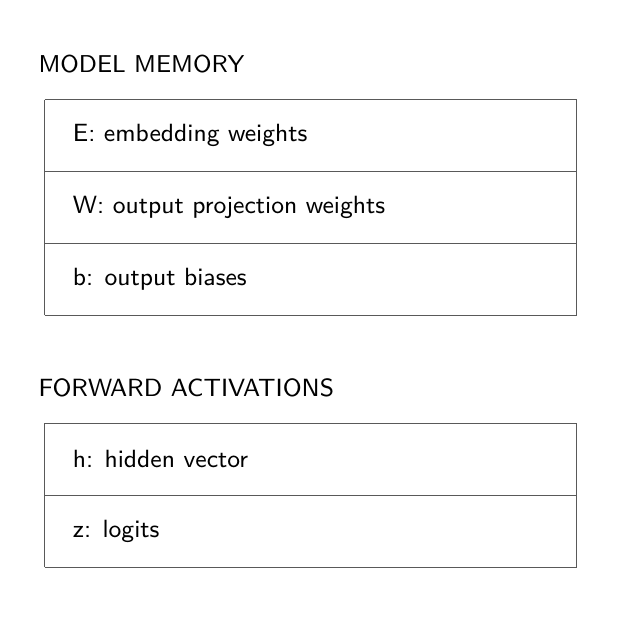
\begin{tikzpicture}[x=6.2pt,y=-13pt,draw=black!65,line width=.45pt]
\path[use as bounding box] (-1,-1) rectangle (33,15);
\node[anchor=west,inner sep=0pt,font=\sffamily\fontsize{9}{11}\selectfont] at (-0.4,0) {\begin{adjustbox}{max width=74.4pt}MODEL MEMORY\end{adjustbox}};
\draw (0,1) -- (0.5,1);
\draw (0,1) -- (0,1.5);
\draw (1,1) -- (0.5,1);
\draw (1,1) -- (1.5,1);
\draw (2,1) -- (1.5,1);
\draw (2,1) -- (2.5,1);
\draw (3,1) -- (2.5,1);
\draw (3,1) -- (3.5,1);
\draw (4,1) -- (3.5,1);
\draw (4,1) -- (4.5,1);
\draw (5,1) -- (4.5,1);
\draw (5,1) -- (5.5,1);
\draw (6,1) -- (5.5,1);
\draw (6,1) -- (6.5,1);
\draw (7,1) -- (6.5,1);
\draw (7,1) -- (7.5,1);
\draw (8,1) -- (7.5,1);
\draw (8,1) -- (8.5,1);
\draw (9,1) -- (8.5,1);
\draw (9,1) -- (9.5,1);
\draw (10,1) -- (9.5,1);
\draw (10,1) -- (10.5,1);
\draw (11,1) -- (10.5,1);
\draw (11,1) -- (11.5,1);
\draw (12,1) -- (11.5,1);
\draw (12,1) -- (12.5,1);
\draw (13,1) -- (12.5,1);
\draw (13,1) -- (13.5,1);
\draw (14,1) -- (13.5,1);
\draw (14,1) -- (14.5,1);
\draw (15,1) -- (14.5,1);
\draw (15,1) -- (15.5,1);
\draw (16,1) -- (15.5,1);
\draw (16,1) -- (16.5,1);
\draw (17,1) -- (16.5,1);
\draw (17,1) -- (17.5,1);
\draw (18,1) -- (17.5,1);
\draw (18,1) -- (18.5,1);
\draw (19,1) -- (18.5,1);
\draw (19,1) -- (19.5,1);
\draw (20,1) -- (19.5,1);
\draw (20,1) -- (20.5,1);
\draw (21,1) -- (20.5,1);
\draw (21,1) -- (21.5,1);
\draw (22,1) -- (21.5,1);
\draw (22,1) -- (22.5,1);
\draw (23,1) -- (22.5,1);
\draw (23,1) -- (23.5,1);
\draw (24,1) -- (23.5,1);
\draw (24,1) -- (24.5,1);
\draw (25,1) -- (24.5,1);
\draw (25,1) -- (25.5,1);
\draw (26,1) -- (25.5,1);
\draw (26,1) -- (26.5,1);
\draw (27,1) -- (26.5,1);
\draw (27,1) -- (27.5,1);
\draw (28,1) -- (27.5,1);
\draw (28,1) -- (28.5,1);
\draw (29,1) -- (28.5,1);
\draw (29,1) -- (29.5,1);
\draw (30,1) -- (29.5,1);
\draw (30,1) -- (30.5,1);
\draw (31,1) -- (30.5,1);
\draw (31,1) -- (31,1.5);
\draw (0,2) -- (0,1.5);
\draw (0,2) -- (0,2.5);
\draw (31,2) -- (31,1.5);
\draw (31,2) -- (31,2.5);
\node[anchor=west,inner sep=0pt,font=\sffamily\fontsize{9}{11}\selectfont] at (1.6,2) {\begin{adjustbox}{max width=124.0pt}E: embedding weights\end{adjustbox}};
\draw (0,3) -- (0,2.5);
\draw (0,3) -- (0.5,3);
\draw (0,3) -- (0,3.5);
\draw (1,3) -- (0.5,3);
\draw (1,3) -- (1.5,3);
\draw (2,3) -- (1.5,3);
\draw (2,3) -- (2.5,3);
\draw (3,3) -- (2.5,3);
\draw (3,3) -- (3.5,3);
\draw (4,3) -- (3.5,3);
\draw (4,3) -- (4.5,3);
\draw (5,3) -- (4.5,3);
\draw (5,3) -- (5.5,3);
\draw (6,3) -- (5.5,3);
\draw (6,3) -- (6.5,3);
\draw (7,3) -- (6.5,3);
\draw (7,3) -- (7.5,3);
\draw (8,3) -- (7.5,3);
\draw (8,3) -- (8.5,3);
\draw (9,3) -- (8.5,3);
\draw (9,3) -- (9.5,3);
\draw (10,3) -- (9.5,3);
\draw (10,3) -- (10.5,3);
\draw (11,3) -- (10.5,3);
\draw (11,3) -- (11.5,3);
\draw (12,3) -- (11.5,3);
\draw (12,3) -- (12.5,3);
\draw (13,3) -- (12.5,3);
\draw (13,3) -- (13.5,3);
\draw (14,3) -- (13.5,3);
\draw (14,3) -- (14.5,3);
\draw (15,3) -- (14.5,3);
\draw (15,3) -- (15.5,3);
\draw (16,3) -- (15.5,3);
\draw (16,3) -- (16.5,3);
\draw (17,3) -- (16.5,3);
\draw (17,3) -- (17.5,3);
\draw (18,3) -- (17.5,3);
\draw (18,3) -- (18.5,3);
\draw (19,3) -- (18.5,3);
\draw (19,3) -- (19.5,3);
\draw (20,3) -- (19.5,3);
\draw (20,3) -- (20.5,3);
\draw (21,3) -- (20.5,3);
\draw (21,3) -- (21.5,3);
\draw (22,3) -- (21.5,3);
\draw (22,3) -- (22.5,3);
\draw (23,3) -- (22.5,3);
\draw (23,3) -- (23.5,3);
\draw (24,3) -- (23.5,3);
\draw (24,3) -- (24.5,3);
\draw (25,3) -- (24.5,3);
\draw (25,3) -- (25.5,3);
\draw (26,3) -- (25.5,3);
\draw (26,3) -- (26.5,3);
\draw (27,3) -- (26.5,3);
\draw (27,3) -- (27.5,3);
\draw (28,3) -- (27.5,3);
\draw (28,3) -- (28.5,3);
\draw (29,3) -- (28.5,3);
\draw (29,3) -- (29.5,3);
\draw (30,3) -- (29.5,3);
\draw (30,3) -- (30.5,3);
\draw (31,3) -- (31,2.5);
\draw (31,3) -- (30.5,3);
\draw (31,3) -- (31,3.5);
\draw (0,4) -- (0,3.5);
\draw (0,4) -- (0,4.5);
\draw (31,4) -- (31,3.5);
\draw (31,4) -- (31,4.5);
\node[anchor=west,inner sep=0pt,font=\sffamily\fontsize{9}{11}\selectfont] at (1.6,4) {\begin{adjustbox}{max width=173.6pt}W: output projection weights\end{adjustbox}};
\draw (0,5) -- (0,4.5);
\draw (0,5) -- (0.5,5);
\draw (0,5) -- (0,5.5);
\draw (1,5) -- (0.5,5);
\draw (1,5) -- (1.5,5);
\draw (2,5) -- (1.5,5);
\draw (2,5) -- (2.5,5);
\draw (3,5) -- (2.5,5);
\draw (3,5) -- (3.5,5);
\draw (4,5) -- (3.5,5);
\draw (4,5) -- (4.5,5);
\draw (5,5) -- (4.5,5);
\draw (5,5) -- (5.5,5);
\draw (6,5) -- (5.5,5);
\draw (6,5) -- (6.5,5);
\draw (7,5) -- (6.5,5);
\draw (7,5) -- (7.5,5);
\draw (8,5) -- (7.5,5);
\draw (8,5) -- (8.5,5);
\draw (9,5) -- (8.5,5);
\draw (9,5) -- (9.5,5);
\draw (10,5) -- (9.5,5);
\draw (10,5) -- (10.5,5);
\draw (11,5) -- (10.5,5);
\draw (11,5) -- (11.5,5);
\draw (12,5) -- (11.5,5);
\draw (12,5) -- (12.5,5);
\draw (13,5) -- (12.5,5);
\draw (13,5) -- (13.5,5);
\draw (14,5) -- (13.5,5);
\draw (14,5) -- (14.5,5);
\draw (15,5) -- (14.5,5);
\draw (15,5) -- (15.5,5);
\draw (16,5) -- (15.5,5);
\draw (16,5) -- (16.5,5);
\draw (17,5) -- (16.5,5);
\draw (17,5) -- (17.5,5);
\draw (18,5) -- (17.5,5);
\draw (18,5) -- (18.5,5);
\draw (19,5) -- (18.5,5);
\draw (19,5) -- (19.5,5);
\draw (20,5) -- (19.5,5);
\draw (20,5) -- (20.5,5);
\draw (21,5) -- (20.5,5);
\draw (21,5) -- (21.5,5);
\draw (22,5) -- (21.5,5);
\draw (22,5) -- (22.5,5);
\draw (23,5) -- (22.5,5);
\draw (23,5) -- (23.5,5);
\draw (24,5) -- (23.5,5);
\draw (24,5) -- (24.5,5);
\draw (25,5) -- (24.5,5);
\draw (25,5) -- (25.5,5);
\draw (26,5) -- (25.5,5);
\draw (26,5) -- (26.5,5);
\draw (27,5) -- (26.5,5);
\draw (27,5) -- (27.5,5);
\draw (28,5) -- (27.5,5);
\draw (28,5) -- (28.5,5);
\draw (29,5) -- (28.5,5);
\draw (29,5) -- (29.5,5);
\draw (30,5) -- (29.5,5);
\draw (30,5) -- (30.5,5);
\draw (31,5) -- (31,4.5);
\draw (31,5) -- (30.5,5);
\draw (31,5) -- (31,5.5);
\draw (0,6) -- (0,5.5);
\draw (0,6) -- (0,6.5);
\draw (31,6) -- (31,5.5);
\draw (31,6) -- (31,6.5);
\node[anchor=west,inner sep=0pt,font=\sffamily\fontsize{9}{11}\selectfont] at (1.6,6) {\begin{adjustbox}{max width=99.2pt}b: output biases\end{adjustbox}};
\draw (0,7) -- (0.5,7);
\draw (0,7) -- (0,6.5);
\draw (1,7) -- (0.5,7);
\draw (1,7) -- (1.5,7);
\draw (2,7) -- (1.5,7);
\draw (2,7) -- (2.5,7);
\draw (3,7) -- (2.5,7);
\draw (3,7) -- (3.5,7);
\draw (4,7) -- (3.5,7);
\draw (4,7) -- (4.5,7);
\draw (5,7) -- (4.5,7);
\draw (5,7) -- (5.5,7);
\draw (6,7) -- (5.5,7);
\draw (6,7) -- (6.5,7);
\draw (7,7) -- (6.5,7);
\draw (7,7) -- (7.5,7);
\draw (8,7) -- (7.5,7);
\draw (8,7) -- (8.5,7);
\draw (9,7) -- (8.5,7);
\draw (9,7) -- (9.5,7);
\draw (10,7) -- (9.5,7);
\draw (10,7) -- (10.5,7);
\draw (11,7) -- (10.5,7);
\draw (11,7) -- (11.5,7);
\draw (12,7) -- (11.5,7);
\draw (12,7) -- (12.5,7);
\draw (13,7) -- (12.5,7);
\draw (13,7) -- (13.5,7);
\draw (14,7) -- (13.5,7);
\draw (14,7) -- (14.5,7);
\draw (15,7) -- (14.5,7);
\draw (15,7) -- (15.5,7);
\draw (16,7) -- (15.5,7);
\draw (16,7) -- (16.5,7);
\draw (17,7) -- (16.5,7);
\draw (17,7) -- (17.5,7);
\draw (18,7) -- (17.5,7);
\draw (18,7) -- (18.5,7);
\draw (19,7) -- (18.5,7);
\draw (19,7) -- (19.5,7);
\draw (20,7) -- (19.5,7);
\draw (20,7) -- (20.5,7);
\draw (21,7) -- (20.5,7);
\draw (21,7) -- (21.5,7);
\draw (22,7) -- (21.5,7);
\draw (22,7) -- (22.5,7);
\draw (23,7) -- (22.5,7);
\draw (23,7) -- (23.5,7);
\draw (24,7) -- (23.5,7);
\draw (24,7) -- (24.5,7);
\draw (25,7) -- (24.5,7);
\draw (25,7) -- (25.5,7);
\draw (26,7) -- (25.5,7);
\draw (26,7) -- (26.5,7);
\draw (27,7) -- (26.5,7);
\draw (27,7) -- (27.5,7);
\draw (28,7) -- (27.5,7);
\draw (28,7) -- (28.5,7);
\draw (29,7) -- (28.5,7);
\draw (29,7) -- (29.5,7);
\draw (30,7) -- (29.5,7);
\draw (30,7) -- (30.5,7);
\draw (31,7) -- (30.5,7);
\draw (31,7) -- (31,6.5);
\node[anchor=west,inner sep=0pt,font=\sffamily\fontsize{9}{11}\selectfont] at (-0.4,9) {\begin{adjustbox}{max width=117.8pt}FORWARD ACTIVATIONS\end{adjustbox}};
\draw (0,10) -- (0.5,10);
\draw (0,10) -- (0,10.5);
\draw (1,10) -- (0.5,10);
\draw (1,10) -- (1.5,10);
\draw (2,10) -- (1.5,10);
\draw (2,10) -- (2.5,10);
\draw (3,10) -- (2.5,10);
\draw (3,10) -- (3.5,10);
\draw (4,10) -- (3.5,10);
\draw (4,10) -- (4.5,10);
\draw (5,10) -- (4.5,10);
\draw (5,10) -- (5.5,10);
\draw (6,10) -- (5.5,10);
\draw (6,10) -- (6.5,10);
\draw (7,10) -- (6.5,10);
\draw (7,10) -- (7.5,10);
\draw (8,10) -- (7.5,10);
\draw (8,10) -- (8.5,10);
\draw (9,10) -- (8.5,10);
\draw (9,10) -- (9.5,10);
\draw (10,10) -- (9.5,10);
\draw (10,10) -- (10.5,10);
\draw (11,10) -- (10.5,10);
\draw (11,10) -- (11.5,10);
\draw (12,10) -- (11.5,10);
\draw (12,10) -- (12.5,10);
\draw (13,10) -- (12.5,10);
\draw (13,10) -- (13.5,10);
\draw (14,10) -- (13.5,10);
\draw (14,10) -- (14.5,10);
\draw (15,10) -- (14.5,10);
\draw (15,10) -- (15.5,10);
\draw (16,10) -- (15.5,10);
\draw (16,10) -- (16.5,10);
\draw (17,10) -- (16.5,10);
\draw (17,10) -- (17.5,10);
\draw (18,10) -- (17.5,10);
\draw (18,10) -- (18.5,10);
\draw (19,10) -- (18.5,10);
\draw (19,10) -- (19.5,10);
\draw (20,10) -- (19.5,10);
\draw (20,10) -- (20.5,10);
\draw (21,10) -- (20.5,10);
\draw (21,10) -- (21.5,10);
\draw (22,10) -- (21.5,10);
\draw (22,10) -- (22.5,10);
\draw (23,10) -- (22.5,10);
\draw (23,10) -- (23.5,10);
\draw (24,10) -- (23.5,10);
\draw (24,10) -- (24.5,10);
\draw (25,10) -- (24.5,10);
\draw (25,10) -- (25.5,10);
\draw (26,10) -- (25.5,10);
\draw (26,10) -- (26.5,10);
\draw (27,10) -- (26.5,10);
\draw (27,10) -- (27.5,10);
\draw (28,10) -- (27.5,10);
\draw (28,10) -- (28.5,10);
\draw (29,10) -- (28.5,10);
\draw (29,10) -- (29.5,10);
\draw (30,10) -- (29.5,10);
\draw (30,10) -- (30.5,10);
\draw (31,10) -- (30.5,10);
\draw (31,10) -- (31,10.5);
\draw (0,11) -- (0,10.5);
\draw (0,11) -- (0,11.5);
\draw (31,11) -- (31,10.5);
\draw (31,11) -- (31,11.5);
\node[anchor=west,inner sep=0pt,font=\sffamily\fontsize{9}{11}\selectfont] at (1.6,11) {\begin{adjustbox}{max width=99.2pt}h: hidden vector\end{adjustbox}};
\draw (0,12) -- (0,11.5);
\draw (0,12) -- (0.5,12);
\draw (0,12) -- (0,12.5);
\draw (1,12) -- (0.5,12);
\draw (1,12) -- (1.5,12);
\draw (2,12) -- (1.5,12);
\draw (2,12) -- (2.5,12);
\draw (3,12) -- (2.5,12);
\draw (3,12) -- (3.5,12);
\draw (4,12) -- (3.5,12);
\draw (4,12) -- (4.5,12);
\draw (5,12) -- (4.5,12);
\draw (5,12) -- (5.5,12);
\draw (6,12) -- (5.5,12);
\draw (6,12) -- (6.5,12);
\draw (7,12) -- (6.5,12);
\draw (7,12) -- (7.5,12);
\draw (8,12) -- (7.5,12);
\draw (8,12) -- (8.5,12);
\draw (9,12) -- (8.5,12);
\draw (9,12) -- (9.5,12);
\draw (10,12) -- (9.5,12);
\draw (10,12) -- (10.5,12);
\draw (11,12) -- (10.5,12);
\draw (11,12) -- (11.5,12);
\draw (12,12) -- (11.5,12);
\draw (12,12) -- (12.5,12);
\draw (13,12) -- (12.5,12);
\draw (13,12) -- (13.5,12);
\draw (14,12) -- (13.5,12);
\draw (14,12) -- (14.5,12);
\draw (15,12) -- (14.5,12);
\draw (15,12) -- (15.5,12);
\draw (16,12) -- (15.5,12);
\draw (16,12) -- (16.5,12);
\draw (17,12) -- (16.5,12);
\draw (17,12) -- (17.5,12);
\draw (18,12) -- (17.5,12);
\draw (18,12) -- (18.5,12);
\draw (19,12) -- (18.5,12);
\draw (19,12) -- (19.5,12);
\draw (20,12) -- (19.5,12);
\draw (20,12) -- (20.5,12);
\draw (21,12) -- (20.5,12);
\draw (21,12) -- (21.5,12);
\draw (22,12) -- (21.5,12);
\draw (22,12) -- (22.5,12);
\draw (23,12) -- (22.5,12);
\draw (23,12) -- (23.5,12);
\draw (24,12) -- (23.5,12);
\draw (24,12) -- (24.5,12);
\draw (25,12) -- (24.5,12);
\draw (25,12) -- (25.5,12);
\draw (26,12) -- (25.5,12);
\draw (26,12) -- (26.5,12);
\draw (27,12) -- (26.5,12);
\draw (27,12) -- (27.5,12);
\draw (28,12) -- (27.5,12);
\draw (28,12) -- (28.5,12);
\draw (29,12) -- (28.5,12);
\draw (29,12) -- (29.5,12);
\draw (30,12) -- (29.5,12);
\draw (30,12) -- (30.5,12);
\draw (31,12) -- (31,11.5);
\draw (31,12) -- (30.5,12);
\draw (31,12) -- (31,12.5);
\draw (0,13) -- (0,12.5);
\draw (0,13) -- (0,13.5);
\draw (31,13) -- (31,12.5);
\draw (31,13) -- (31,13.5);
\node[anchor=west,inner sep=0pt,font=\sffamily\fontsize{9}{11}\selectfont] at (1.6,13) {\begin{adjustbox}{max width=55.800000000000004pt}z: logits\end{adjustbox}};
\draw (0,14) -- (0.5,14);
\draw (0,14) -- (0,13.5);
\draw (1,14) -- (0.5,14);
\draw (1,14) -- (1.5,14);
\draw (2,14) -- (1.5,14);
\draw (2,14) -- (2.5,14);
\draw (3,14) -- (2.5,14);
\draw (3,14) -- (3.5,14);
\draw (4,14) -- (3.5,14);
\draw (4,14) -- (4.5,14);
\draw (5,14) -- (4.5,14);
\draw (5,14) -- (5.5,14);
\draw (6,14) -- (5.5,14);
\draw (6,14) -- (6.5,14);
\draw (7,14) -- (6.5,14);
\draw (7,14) -- (7.5,14);
\draw (8,14) -- (7.5,14);
\draw (8,14) -- (8.5,14);
\draw (9,14) -- (8.5,14);
\draw (9,14) -- (9.5,14);
\draw (10,14) -- (9.5,14);
\draw (10,14) -- (10.5,14);
\draw (11,14) -- (10.5,14);
\draw (11,14) -- (11.5,14);
\draw (12,14) -- (11.5,14);
\draw (12,14) -- (12.5,14);
\draw (13,14) -- (12.5,14);
\draw (13,14) -- (13.5,14);
\draw (14,14) -- (13.5,14);
\draw (14,14) -- (14.5,14);
\draw (15,14) -- (14.5,14);
\draw (15,14) -- (15.5,14);
\draw (16,14) -- (15.5,14);
\draw (16,14) -- (16.5,14);
\draw (17,14) -- (16.5,14);
\draw (17,14) -- (17.5,14);
\draw (18,14) -- (17.5,14);
\draw (18,14) -- (18.5,14);
\draw (19,14) -- (18.5,14);
\draw (19,14) -- (19.5,14);
\draw (20,14) -- (19.5,14);
\draw (20,14) -- (20.5,14);
\draw (21,14) -- (20.5,14);
\draw (21,14) -- (21.5,14);
\draw (22,14) -- (21.5,14);
\draw (22,14) -- (22.5,14);
\draw (23,14) -- (22.5,14);
\draw (23,14) -- (23.5,14);
\draw (24,14) -- (23.5,14);
\draw (24,14) -- (24.5,14);
\draw (25,14) -- (24.5,14);
\draw (25,14) -- (25.5,14);
\draw (26,14) -- (25.5,14);
\draw (26,14) -- (26.5,14);
\draw (27,14) -- (26.5,14);
\draw (27,14) -- (27.5,14);
\draw (28,14) -- (27.5,14);
\draw (28,14) -- (28.5,14);
\draw (29,14) -- (28.5,14);
\draw (29,14) -- (29.5,14);
\draw (30,14) -- (29.5,14);
\draw (30,14) -- (30.5,14);
\draw (31,14) -- (30.5,14);
\draw (31,14) -- (31,13.5);
\end{tikzpicture}
\end{adjustbox}\end{center}

No ``hidden reasoning'' is stored here. The adjective \emph{hidden}
distinguishes an internal representation from observable input and
output. It does not imply a human-readable chain of thought.

\subsection{Follow the token, byte, and
owner}\label{follow-the-token-byte-and-owner}

The
\href{https://github.com/hermonai/inside-the-llm-engine/blob/astra-visual-rewrite/diagrams/model/token-id-to-logits.txt}{complete
Chapter 3 path} extends our first recurring journey:

\begin{center}\begin{adjustbox}{max width=\linewidth}% Legacy topology preserved as native vectors and typeset labels.
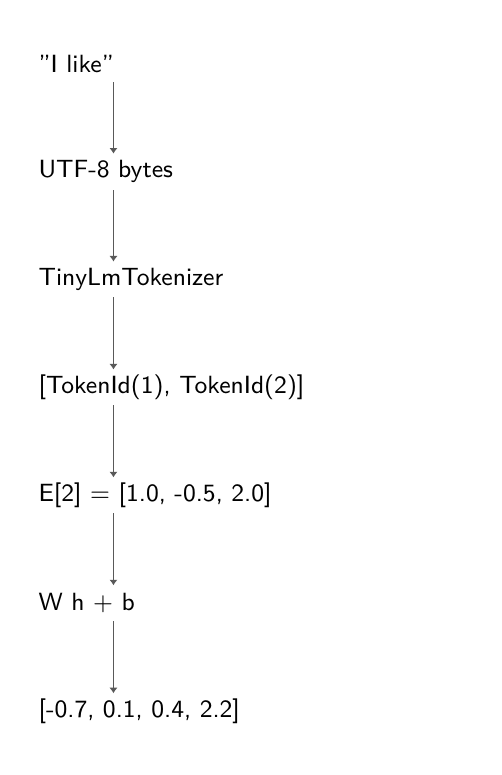
\begin{tikzpicture}[x=6.2pt,y=-13pt,draw=black!65,line width=.45pt]
\path[use as bounding box] (-1,-1) rectangle (25,19);
\node[anchor=west,inner sep=0pt,font=\sffamily\fontsize{9}{11}\selectfont] at (-0.4,0) {\begin{adjustbox}{max width=49.6pt}"I like"\end{adjustbox}};
\draw (4,1) -- (4,0.5);
\draw (4,1) -- (4,1.5);
\draw[-{Latex[length=2pt,width=3pt]}] (4,1.5) -- (4,2.5);
\node[anchor=west,inner sep=0pt,font=\sffamily\fontsize{9}{11}\selectfont] at (-0.4,3) {\begin{adjustbox}{max width=68.2pt}UTF-8 bytes\end{adjustbox}};
\draw (4,4) -- (4,3.5);
\draw (4,4) -- (4,4.5);
\draw[-{Latex[length=2pt,width=3pt]}] (4,4.5) -- (4,5.5);
\node[anchor=west,inner sep=0pt,font=\sffamily\fontsize{9}{11}\selectfont] at (-0.4,6) {\begin{adjustbox}{max width=93.0pt}TinyLmTokenizer\end{adjustbox}};
\draw (4,7) -- (4,6.5);
\draw (4,7) -- (4,7.5);
\draw[-{Latex[length=2pt,width=3pt]}] (4,7.5) -- (4,8.5);
\node[anchor=west,inner sep=0pt,font=\sffamily\fontsize{9}{11}\selectfont] at (-0.4,9) {\begin{adjustbox}{max width=148.8pt}[TokenId(1), TokenId(2)]\end{adjustbox}};
\draw (4,10) -- (4,9.5);
\draw (4,10) -- (4,10.5);
\draw[-{Latex[length=2pt,width=3pt]}] (4,10.5) -- (4,11.5);
\node[anchor=west,inner sep=0pt,font=\sffamily\fontsize{9}{11}\selectfont] at (-0.4,12) {\begin{adjustbox}{max width=142.6pt}E[2] = [1.0, -0.5, 2.0]\end{adjustbox}};
\draw (4,13) -- (4,12.5);
\draw (4,13) -- (4,13.5);
\draw[-{Latex[length=2pt,width=3pt]}] (4,13.5) -- (4,14.5);
\node[anchor=west,inner sep=0pt,font=\sffamily\fontsize{9}{11}\selectfont] at (-0.4,15) {\begin{adjustbox}{max width=43.4pt}W h + b\end{adjustbox}};
\draw (4,16) -- (4,15.5);
\draw (4,16) -- (4,16.5);
\draw[-{Latex[length=2pt,width=3pt]}] (4,16.5) -- (4,17.5);
\node[anchor=west,inner sep=0pt,font=\sffamily\fontsize{9}{11}\selectfont] at (-0.4,18) {\begin{adjustbox}{max width=130.20000000000002pt}[-0.7, 0.1, 0.4, 2.2]\end{adjustbox}};
\end{tikzpicture}
\end{adjustbox}\end{center}

Follow one parameter byte conceptually. It begins as a fixture literal.
Model construction places it in a contiguous
\texttt{Vec\textless{}f32\textgreater{}}. A forward call calculates its
row-major offset, the CPU loads it, multiplies it by one hidden value,
and adds the product to an \texttt{f32} accumulator. Later chapters will
replace source literals with model-file bytes and may replace scalar
loads with packed SIMD or device operations. The ownership and
interpretation trail must remain auditable.

Follow the owner. \texttt{\seqsplit{TinyLanguageModel}} owns \texttt{E},
\texttt{W}, \texttt{b}, \texttt{V}, and \texttt{D}. A \texttt{Request}
owns its input token sequence and generation budget. The forward result
owns \texttt{h} and typed \texttt{Logits}. The runtime owns generated
token history, the UTF-8 buffer, ordered stream emissions, timings, and
the only terminal transition. The selector borrows logits and returns an
identity; it owns neither parameters nor activations.

\subsection{Count the parameters before counting
performance}\label{count-the-parameters-before-counting-performance}

The embedding contains \(V_{\mathrm{vocab}}D\) parameters. The untied
output projection contains another \(V_{\mathrm{vocab}}D\). The bias
contains \(V_{\mathrm{vocab}}\). Therefore:

\[
N_{\mathrm{param}}
=V_{\mathrm{vocab}}D+V_{\mathrm{vocab}}D+V_{\mathrm{vocab}}
=2V_{\mathrm{vocab}}D+V_{\mathrm{vocab}}.
\]

With \texttt{f32}, each parameter occupies four bytes:

\[
B_{\mathrm{param}}
=4\left(2V_{\mathrm{vocab}}D+V_{\mathrm{vocab}}\right)
\quad[\mathrm{bytes}].
\]

For ENGINE-1, \(V_{\mathrm{vocab}}=4\) and \(D=3\):

\[
N_{\mathrm{param}}=2(4)(3)+4=28,
\qquad B_{\mathrm{param}}=28(4)=112\ \mathrm{bytes}.
\]

This count excludes \texttt{Vec} metadata, allocator bookkeeping,
dimensions, code, and forward activations. It describes parameter
payload only. The hidden activation uses \texttt{D*4\ =\ 12} bytes of
\texttt{f32} payload; the logits use \texttt{V*4\ =\ 16}.

The same formulas produce a useful scale table:

{\def\LTcaptype{none} % do not increment counter
\begin{longtable}[]{@{}
  >{\raggedleft\arraybackslash}p{(\linewidth - 10\tabcolsep) * \real{0.1667}}
  >{\raggedleft\arraybackslash}p{(\linewidth - 10\tabcolsep) * \real{0.1667}}
  >{\raggedleft\arraybackslash}p{(\linewidth - 10\tabcolsep) * \real{0.1667}}
  >{\raggedleft\arraybackslash}p{(\linewidth - 10\tabcolsep) * \real{0.1667}}
  >{\raggedleft\arraybackslash}p{(\linewidth - 10\tabcolsep) * \real{0.1667}}
  >{\raggedleft\arraybackslash}p{(\linewidth - 10\tabcolsep) * \real{0.1667}}@{}}
\toprule\noalign{}
\begin{minipage}[b]{\linewidth}\raggedleft
\texttt{V}
\end{minipage} & \begin{minipage}[b]{\linewidth}\raggedleft
\texttt{D}
\end{minipage} & \begin{minipage}[b]{\linewidth}\raggedleft
\texttt{E} parameters
\end{minipage} & \begin{minipage}[b]{\linewidth}\raggedleft
\texttt{W} parameters
\end{minipage} & \begin{minipage}[b]{\linewidth}\raggedleft
Total \texttt{2VD+V}
\end{minipage} & \begin{minipage}[b]{\linewidth}\raggedleft
\texttt{f32} bytes
\end{minipage} \\
\midrule\noalign{}
\endhead
\bottomrule\noalign{}
\endlastfoot
4 & 3 & 12 & 12 & 28 & 112 \\
100 & 16 & 1,600 & 1,600 & 3,300 & 13,200 \\
50,000 & 4,096 & 204,800,000 & 204,800,000 & 409,650,000 &
1,638,600,000 \\
\end{longtable}
}

The formula scales quickly. Consider a hypothetical vocabulary of 50,000
and hidden dimension 4,096 under this same simplified, untied
architecture:

\[
\begin{aligned}
V_{\mathrm{vocab}}D&=50{,}000(4{,}096)=204{,}800{,}000,\\
N_{\mathrm{param}}&=409{,}650{,}000,\\
B_{\mathrm{param}}&=1{,}638{,}600{,}000\ \mathrm{bytes}
\approx1.526\ \mathrm{GiB}.
\end{aligned}
\]

That is not the size of a complete real language model and not a
measurement. It isolates vocabulary embedding and projection under
stated assumptions. It does explain why output heads are not negligible
and why real designs care about lower-precision storage, quantization,
and optimized multiplication.

Some models use \textbf{weight tying}: the input embedding and output
projection reuse the same parameter storage, with the orientation
interpreted according to the chosen convention. That can eliminate one
\texttt{V*D} parameter collection. It is an architectural option, not a
universal law. ENGINE-1 leaves \texttt{E} and \texttt{W} separate
because changing an input representation and changing a candidate
scoring row should be visibly different experiments.

\subsection{Count the work and the bytes
read}\label{count-the-work-and-the-bytes-read}

Embedding lookup performs little arithmetic. It validates \texttt{x},
computes an offset, and reads one row: \texttt{D} parameter values. It
does not scan all \texttt{V} rows.

Output projection is different. For each of \texttt{V} output rows, it
performs \texttt{D} multiplications and approximately \texttt{D}
additions including bias accumulation. The work grows as

\[
\Theta\!\left(V_{\mathrm{vocab}}D\right)
\]

for this exact dense projection: every output row and hidden component
is visited once.

For one forward call, the scalar kernel reads essentially all
\texttt{V*D} projection weights and \texttt{V} biases and writes
\texttt{V} logits. It reuses the small hidden vector across all rows.
Even in this tiny model, two distinct systems patterns appear:

\begin{itemize}
\tightlist
\item
  embedding lookup: sparse row access, little arithmetic;
\item
  output projection: broad weight access plus many dot-product
  operations.
\end{itemize}

Inference performance depends on computation and data movement. A
processor cannot multiply a weight it has not obtained through its
memory hierarchy. Later chapters will ask whether a kernel is limited by
arithmetic, weight bandwidth, cache reuse, conversion, launch cost,
synchronization, or another resource. Chapter 3 establishes the
accounting habit without pretending that a 4-by-3 loop predicts a
production workload.

The repository includes
\texttt{\seqsplit{code/experiments/chapter-03-projection-scaling.py}}.
It varies modest \texttt{V} and \texttt{D}, reports parameter payload
and median time for a plain-Python scalar loop, and prints a checksum.
Its result record is in
\texttt{\seqsplit{research/benchmarks/chapter-03-projection-scaling.md}}.

\begin{quote}
\textbf{PERFORMANCE LAB} The scaling probe is pedagogical. It shows that
larger shapes create more stored values and loop iterations in that
harness. Python interpreter timing does not predict Rust, BLAS, SIMD,
GPU, or real-model throughput, and it must not be compared with Hermon
or llama.cpp.
\end{quote}

\subsection{Model semantics are not one
implementation}\label{model-semantics-are-not-one-implementation}

The equations say what the model computes:

\begin{verbatim}
h = E[x]
z = W h + b
\end{verbatim}

The scalar Rust loops say how ENGINE-1 executes those semantics today.
The
\href{https://github.com/hermonai/inside-the-llm-engine/blob/astra-visual-rewrite/diagrams/model/semantics-vs-execution.txt}{semantics/execution
diagram} keeps that line visible:

\begin{verbatim}
                 MODEL SEMANTICS
TokenId -> embedding -> hidden -> projection -> logits
=======================================================
              EXECUTION IMPLEMENTATION
today: scalar row-major Rust loops
later: CPU SIMD, Metal, CUDA, other native kernels
\end{verbatim}

An optimized implementation may load several weights into vector
registers, tile a matrix, use a quantized packed layout, fuse
operations, or dispatch to a device. It can allocate scratch
differently. None of those choices may change which token owns a row,
transpose the mathematical convention accidentally, drop the bias, or
produce errors outside the declared numerical tolerance.

\begin{quote}
\textbf{FIRST PRINCIPLE} An engine may change execution while preserving
model semantics. The oracle defines what must remain invariant.
\end{quote}

This separation is the foundation of later differential testing. The
clarity path need not be fast. The fast path must agree with an
independent clarity path before its timing is meaningful.

\subsection{BUILD IT: ENGINE-1}\label{build-it-engine-1}

ENGINE-1 evolves the existing Rust crate instead of maintaining parallel
copies of an entire runtime. Git history preserves the exact ENGINE-0
milestone. The current code keeps Chapter 2's tokenizer trait,
chat/template types, request, streaming events, UTF-8 framer,
cancellation contract, timings, and terminal lifecycle. It replaces the
fake numerical center.

\subsubsection{The model structure}\label{the-model-structure}

\texttt{\seqsplit{TinyLanguageModel}} owns:

\begin{verbatim}
pub struct TinyLanguageModel {
    vocab_size: usize,
    hidden_dim: usize,
    embedding: Vec<f32>,
    output_weight: Vec<f32>,
    output_bias: Vec<f32>,
}
\end{verbatim}

The deliberately small structure is not a general tensor framework.
Field names carry the semantic rank and role. Construction checks every
length before the model can execute.

The model trait accepts the full history:

\begin{verbatim}
pub trait Model {
    fn vocabulary_size(&self) -> usize;
    fn forward(&self, input: &[TokenId])
        -> Result<ForwardPass, ModelError>;
}
\end{verbatim}

Why accept a sequence if ENGINE-1 uses only its last element? Passing
only \texttt{last\_token} would be locally narrower, but it would make
the runtime decide which history information matters to the model. The
full borrowed slice keeps next-token history at the model boundary,
introduces no input allocation, and makes the limitation testable.
\texttt{forward} calls \texttt{input.last()} and says so in code. Future
models may consume more positions without changing what a request means.

This is a documented teaching choice, not a claim that every production
model API should use the same signature. Batched engines need shapes,
positions, sequence identifiers, cache handles, and output-row requests
that this method does not express.

\subsubsection{A typed forward result}\label{a-typed-forward-result}

\texttt{ForwardPass} contains:

\begin{verbatim}
input_token: TokenId
hidden:      Vec<f32>
logits:      Logits
\end{verbatim}

Keeping the hidden activation in the teaching result makes trace and
oracle inspection straightforward. A production API might retain it only
in debug mode or place scratch in a reusable context. \texttt{Logits}
wraps its vector and exposes a borrowed slice. This prevents unrelated
code from treating every \texttt{Vec\textless{}f32\textgreater{}} as
interchangeable.

The model owns \texttt{Logits} construction and guarantees finite
values. It returns a typed \texttt{ModelError} for an empty sequence or
out-of-range final token. The selector receives only \texttt{\&Logits},
so it cannot reach into parameters or alter the hidden activation.

\subsubsection{Construction is a correctness
boundary}\label{construction-is-a-correctness-boundary}

\texttt{\seqsplit{TinyLanguageModel::try\_new}} rejects:

\begin{itemize}
\tightlist
\item
  zero vocabulary size;
\item
  zero hidden dimension;
\item
  overflow in \texttt{V*D};
\item
  an embedding length other than \texttt{V*D};
\item
  a projection length other than \texttt{V*D};
\item
  a bias length other than \texttt{V};
\item
  any non-finite parameter.
\end{itemize}

These are load-time properties. Paying once during construction lets the
hot inner loop index validated storage without rechecking every row
length. Forward still checks the request-dependent token ID.

Shape bugs are not cosmetic. If \texttt{W} has 11 values instead of 12,
choosing to truncate would omit a term, choosing to pad would invent a
parameter, and indexing blindly could panic. None preserves the declared
model.

\begin{quote}
\textbf{PROVE IT} Model shape validation is inference correctness.
Malformed parameter counts and vocabulary mismatches must fail before
plausible output can hide them.
\end{quote}

\subsubsection{Vocabulary coupling becomes
numerical}\label{vocabulary-coupling-becomes-numerical}

Chapter 2 established that a tokenizer revision and chat template belong
to a model contract. Chapter 3 adds a numeric equality:

\begin{verbatim}
model vocabulary size
    == tokenizer vocabulary size
    == ModelContract vocabulary size
\end{verbatim}

Embedding row \texttt{i}, logit position \texttt{i}, tokenizer identity
\texttt{i}, and EOS recognition must refer to the same token. A vector
of length four cannot safely consume Chapter 2's sparse byte-BPE IDs,
which extend through 1007.

ENGINE-1 therefore has a deliberately tiny paired tokenizer:

\begin{verbatim}
0 <eos>   special, no ordinary output bytes
1 I       bytes "I"
2 like    bytes " like"
3 Rust    bytes " Rust"
\end{verbatim}

Leading spaces belong to two pieces, allowing \texttt{I\ like\ Rust} to
round-trip. The tokenizer rejects all other text with a byte-offset
error. That narrow domain is honest: four embeddings cannot represent a
thousand-ID vocabulary. Chapter 2's byte tokenizer and BPE remain in the
repository for their own labs; they are not silently remapped into
ENGINE-1.

\texttt{\seqsplit{Runtime::try\_new}} validates the model, tokenizer,
and contract sizes and requires an EOS identity. It cannot admit a
request when the model's fourth logit would mean one token to the model
and another to the decoder.

\subsubsection{The inherited lifecycle}\label{the-inherited-lifecycle}

For prompt \texttt{I\ like}, the tokenizer yields \texttt{{[}1,2{]}}.
The first forward uses the last token 2 and produces the oracle logits.
Temporary argmax selects token 3, which decodes to bytes for
\texttt{Rust}. The runtime emits a token event and then a valid text
event.

The generated token is appended to history. The next forward therefore
ends in token 3. With the fixture's \texttt{Rust} embedding
\texttt{{[}-1.0,0.0,0.0{]}}, the logits are:

\begin{verbatim}
[0.3, -0.2, -0.3, -0.5]
\end{verbatim}

EOS at position 0 is the unique maximum. The runtime recognizes it as a
terminal identity, does not ask for ordinary text bytes, checks that the
UTF-8 buffer is complete, and emits exactly one completed terminal
event.

This two-step behavior is not a disguised step table. Both logit vectors
come from the same immutable \texttt{E}, \texttt{W}, and \texttt{b};
only the input embedding row changes.

The lifecycle retains its earlier failure properties:

\begin{itemize}
\tightlist
\item
  empty input or zero generation budget fails before admission;
\item
  cancellation stops before another model call or token emission;
\item
  model, tokenizer, and UTF-8 failures produce one failed terminal;
\item
  EOS produces no text token event;
\item
  maximum-token termination checks pending UTF-8 bytes;
\item
  no event or trace can occur after terminal;
\item
  one request cannot both complete and fail.
\end{itemize}

Chapter 4 will explain the loop as autoregressive generation. Here it
remains minimal infrastructure needed to prove that the new logit
boundary integrates with established ownership.

\subsubsection{An educational numerical
trace}\label{an-educational-numerical-trace}

Run:

\begin{verbatim}
cd code/mini-engine
cargo run -p engine0 -- --trace 'I like'
\end{verbatim}

The trace names admission and execution, then includes the input token,
hidden shape and values, logit shape and values, selected token, decoded
byte count, streamed text, and terminal reason. ENGINE-1 vectors are
small enough to show completely. This must not become a habit of dumping
future tensors with millions of elements. The trace already names shapes
separately from values; later milestones can retain shapes, dtypes,
selected values, and statistics while bounding payload size.

\subsection{Test the arithmetic, not the
story}\label{test-the-arithmetic-not-the-story}

The Rust suite checks more than one happy result:

\begin{itemize}
\tightlist
\item
  valid construction and exact parameter/byte counts;
\item
  zero \texttt{V}, zero \texttt{D}, and multiplication overflow;
\item
  embedding, projection, and bias count mismatches;
\item
  non-finite parameters;
\item
  empty model input and an ID outside \texttt{0..V};
\item
  exact embedding-row selection;
\item
  the complete oracle logit vector within tolerance;
\item
  bias behavior with a zero embedding;
\item
  negative and zero arithmetic;
\item
  repeatability of the complete forward result;
\item
  identical logits for different histories with the same final token;
\item
  expected different logits for different embedding rows;
\item
  EOS as an ordinary position in the output vector;
\item
  one changed projection weight affecting only its row's logit;
\item
  model/tokenizer/contract vocabulary mismatch;
\item
  runtime cancellation, failure, EOS, max-token, UTF-8, event ordering,
  and exactly-one-terminal behavior.
\end{itemize}

Changing one projection weight is a particularly useful causality test.
For input \texttt{like}, change \texttt{W{[}3,0{]}} from 1.0 to 1.5.
Since \texttt{h\_0=1.0}, only \texttt{z\_3} increases, by 0.5:

\begin{verbatim}
before: [-0.7, 0.1, 0.4, 2.2]
after:  [-0.7, 0.1, 0.4, 2.7]
\end{verbatim}

The embedding does not change. Rows 0 through 2 do not read
\texttt{W{[}3,0{]}}. By contrast, changing one embedding component can
affect every logit because all projection rows consume the shared hidden
component.

Labs 5--8 turn these invariants into exercises: calculate the full pass,
change one weight, prove the context limitation, and break the shape
deliberately.

\subsection{Inside Hermon: the same boundary, industrial
machinery}\label{inside-hermon-the-same-boundary-industrial-machinery}

\begin{quote}
\textbf{INSIDE HERMON --- CURRENT} At inspected commit \texttt{472a44c},
Hermon's default runtime is the continuous- batched path, and real-model
numerical execution is delegated through \texttt{hermon-llamacpp} to
pinned llama.cpp commit \texttt{389ff61}.
\end{quote}

Hermon's default path is not an embedding-plus-one-projection model. It
runs a real model graph with layers, context state, batching, and
hardware backends. The useful comparison is the input/output contract.

\texttt{\seqsplit{crates/hermon-runtime/src/dispatch.rs}} selects
\texttt{\seqsplit{RuntimeMode::Batched}} when
\texttt{\seqsplit{HERMON\_RUNTIME\_MODE}} is absent.
\texttt{\seqsplit{crates/hermon-runtime/src/batched.rs}} owns request
scheduling and assembles token positions from multiple active sequences
into a \texttt{Batch}. Each entry can request that its output logits be
kept. The worker calls one context decode and samples the requested
logit row for each sequence.

The simpler blocking path in
\texttt{\seqsplit{crates/hermon-engine/src/engine.rs}} makes the journey
easy to follow: clear per-request context state, tokenize the prompt,
construct a sampler, call context generation, turn returned token IDs
into pieces, frame UTF-8, and emit text. Inside
\texttt{hermon-llamacpp}, \texttt{Context::decode} passes token IDs
through a C shim to \texttt{llama\_decode}.

The pinned llama.cpp header defines the numerical output contract. After
\texttt{llama\_decode}, logits requested by the batch are stored as
rows; each row has \texttt{n\_vocab} columns.
\texttt{\seqsplit{llama\_get\_logits\_ith}} retrieves one output row.
The context implementation synchronizes pending computation before
returning that result.

Hermon therefore owns substantial systems machinery around the current
forward call---model resolution, runtime choice, batch construction,
scheduling, streaming, and lifecycle---while llama.cpp owns the default
real-model numerical graph and its output-logit storage. A sampler
consumes those logits through the llama.cpp context. ENGINE-1 exposes
\texttt{Logits} directly because the teaching goal is to make that
otherwise industrial boundary visible.

\begin{quote}
\textbf{INSIDE HERMON --- PREVIEW} Hermon's own paged GGUF forward is
present behind \texttt{\seqsplit{HERMON\_RUNTIME\_MODE=paged}} and
\texttt{\seqsplit{HERMON\_PAGED\_GGUF=1}}, with a currently stated
greedy CPU limit. Its real-model differential test compares next-token
behavior with the pinned llama.cpp graph. The gate means this path is
not the default CURRENT numerical engine.
\end{quote}

Hermon also contains tensor, backend, paged-KV, and native-kernel
components. Their existence is \textbf{LIBRARY} evidence unless the
request path selects them. This distinction prevents a common
source-reading error: finding a sophisticated kernel and describing
every production request as if it executes there.

ENGINE-1 resembles none of Hermon's production model architecture. It
does establish the abstract contract both systems need:

\begin{verbatim}
token identities -> model execution -> one vocabulary score per output row
\end{verbatim}

\subsection{The fatal context
limitation}\label{the-fatal-context-limitation}

Return to the approximation:

\begin{verbatim}
P(next | history) is approximated by P(next | final token)
\end{verbatim}

Consider two histories:

\begin{verbatim}
History A: I -> like    -> Rust
History B: I -> dislike -> Rust
\end{verbatim}

Both end in the same \texttt{TokenId} for \texttt{Rust}. ENGINE-1
selects the same \texttt{E{[}Rust{]}}, produces the same hidden vector,
and calculates the same logits. The
\href{https://github.com/hermonai/inside-the-llm-engine/blob/astra-visual-rewrite/diagrams/model/context-limitation.txt}{context
limitation diagram} shows information disappearing at the model
boundary.

This is not merely theoretical. The test
\texttt{\seqsplit{same\_last\_token\_produces\_same\_logits\_despite\_different\_history}}
passes two different-length sequences with different prefixes and the
same final token. It asserts equality of both hidden vectors and the
complete logit vectors. A control with a different final token produces
a different embedding and the expected different logits.

No choice of argmax, softmax, temperature, or sampling can recover
history the model never used. Selection policies operate on the logits
they receive. The missing capability must arise before logits:

\begin{verbatim}
We need a mechanism that makes the representation at the current position
depend on context.
\end{verbatim}

Then stop. Part II will build that mechanism progressively. Jumping
directly to attention here would skip the tensor, multiplication,
normalization, projection, position, and ownership foundations needed to
implement it correctly.

\subsection{Common mistakes}\label{common-mistakes-2}

\textbf{Treating token IDs as ordinal measurements.} IDs are vocabulary
identities. Only their mapping to parameter rows supplies numerical
semantics.

\textbf{Calling embedding lookup a required dense multiplication.}
One-hot multiplication is an equivalent equation, not ENGINE-1's
physical execution. The implementation reads one row.

\textbf{Giving hidden dimensions human definitions.} A hidden vector is
a learned activation consumed by later computation. Individual
coordinates need not have isolated, stable meanings.

\textbf{Calling the hidden vector a probability distribution.} Its
values can be arbitrary finite model activations. They need not be
positive or sum to one.

\textbf{Calling logits probabilities.} Logits are unnormalized scores.
Negative values and totals other than one are normal.

\textbf{Assuming the largest logit has probability one.} Argmax returns
an index. It does not define probability or uncertainty.

\textbf{Calling argmax the model.} The model produces the score vector.
Argmax is one selection policy consuming it.

\textbf{Putting selection inside \texttt{forward}.} Doing so prevents
independent testing of logits and entangles immutable model semantics
with generation policy.

\textbf{Confusing parameters and activations.} \texttt{E}, \texttt{W},
and \texttt{b} persist across requests. \texttt{h} and \texttt{z} belong
to a forward execution.

\textbf{Mutating weights during inference.} Ordinary forward execution
reads the loaded model. Training or adaptation is a separate operation
and ownership contract.

\textbf{Testing only the selected token.} Wrong logit values can
preserve the same argmax. Compare the whole vector with an independent
oracle.

\textbf{Passing anonymous vectors without shape meaning.}
\texttt{Vec\textless{}f32\textgreater{}} says neither whether values are
hidden activations or logits nor which vocabulary owns their positions.
Lightweight types and construction checks carry the contract.

\textbf{Treating shape as prose.} A dimension mismatch changes or
invalidates the computation. Reject it before indexing.

\textbf{Assuming matrix notation specifies memory.}
\texttt{z\ =\ W\ h\ +\ b} does not tell us row-major versus column-major
storage, padding, dtype, location, or ownership.

\subsection{Exercises}\label{exercises-2}

\subsubsection{CHECK}\label{check-2}

\begin{enumerate}
\def\labelenumi{\arabic{enumi}.}
\tightlist
\item
  For \texttt{V=8}, \texttt{D=5}, give the shapes of \texttt{E},
  \texttt{W}, \texttt{b}, \texttt{h}, and \texttt{z}.
\item
  Calculate the untied parameter count and \texttt{f32} payload bytes.
\item
  If input token 6 is valid, how many embedding values does lookup read?
\item
  Explain why logit position 6 and embedding row 6 must share vocabulary
  identity even though they serve different computations.
\end{enumerate}

\subsubsection{BUILD}\label{build-2}

Complete
\href{https://github.com/hermonai/inside-the-llm-engine/blob/astra-visual-rewrite/labs/lab-05-forward-pass-by-hand.md}{Lab
5}. Write all four dot products before running either oracle. Then add a
hand oracle for input \texttt{Rust} and verify
\texttt{\seqsplit{[0.3,-0.2,-0.3,-0.5]}}.

\subsubsection{BREAK}\label{break-2}

Complete
\href{https://github.com/hermonai/inside-the-llm-engine/blob/astra-visual-rewrite/labs/lab-08-break-the-shape.md}{Lab
8}. Try malformed lengths, zero dimensions, a non-finite parameter, an
out-of-range ID, and a vocabulary mismatch. Identify which checks occur
once at model construction and which remain request-dependent.

\subsubsection{EXTEND}\label{extend-2}

Complete
\href{https://github.com/hermonai/inside-the-llm-engine/blob/astra-visual-rewrite/labs/lab-06-change-one-weight.md}{Lab
6} and
\href{https://github.com/hermonai/inside-the-llm-engine/blob/astra-visual-rewrite/labs/lab-07-same-last-token-same-output.md}{Lab
7}. Then add a second small valid fixture with \texttt{V=3},
\texttt{D=2}. Keep all values hand-computable and write the expected
full vector independently before implementing the Rust case.

\subsection{Summary}\label{summary-2}

A token ID contains identity, not geometry. An embedding matrix gives
that identity a \texttt{D}-component numerical representation by
selecting one row. An output projection compares the hidden vector with
one row per vocabulary candidate and adds a bias:

\begin{verbatim}
h = E[x]
z = W h + b
\end{verbatim}

ENGINE-1 makes each shape, dtype, layout, owner, lifetime, and scalar
operation explicit. Its \texttt{V=4}, \texttt{D=3} fixture has 28
parameters occupying 112 bytes of \texttt{f32} payload. For input
\texttt{like}, it produces the independently verified vector:

\begin{verbatim}
[-0.7, 0.1, 0.4, 2.2]
\end{verbatim}

The fake candidate table is gone from the current model path. Model
execution returns typed finite logits; a separate temporary selector
chooses an ID. The request lifecycle, EOS handling, byte decoding,
strict UTF-8 framing, cancellation, failure, and exactly-one-terminal
invariant remain executable.

The model is intentionally inadequate. It uses only the final token, so
any two histories ending in that token produce identical logits. That
failure creates the need for context-dependent representations without
hiding the first numerical inference step behind Transformer complexity.

\subsection{What comes next}\label{what-comes-next}

We now have arbitrary-looking but correct scores:

\begin{verbatim}
[-0.7, 0.1, 0.4, 2.2]
\end{verbatim}

How should an engine turn them into the next token? Chapter
4---\textbf{Logits, Sampling, and the Autoregressive Loop}---will derive
numerically stable softmax, distinguish greedy and categorical
selection, introduce temperature, seeds, top-k and top-p, append the
selected identity to history, execute the model again, and reconcile EOS
and token limits with terminal ownership.

The separation established here must survive:

\begin{verbatim}
model semantics -> logits -> logits processing -> sampler -> runtime stopping
\end{verbatim}

Chapter 4 will not have to invent logits or guess what they mean. It can
begin at a typed, oracle-verified full vocabulary vector.

\subsection{References}\label{references}

\begin{itemize}
\tightlist
\item
  Yoshua Bengio, Réjean Ducharme, Pascal Vincent, and Christian Jauvin,
  \href{https://jmlr.org/papers/v3/bengio03a.html}{``A Neural
  Probabilistic Language Model''}, \emph{Journal of Machine Learning
  Research} 3, 2003.
\item
  PyTorch,
  \href{https://docs.pytorch.org/docs/stable/generated/torch.nn.Embedding}{\texttt{\seqsplit{torch.nn.Embedding}}},
  official lookup-table contract, inspected 2026-09-02.
\item
  PyTorch,
  \href{https://docs.pytorch.org/docs/stable/generated/torch.nn.Linear.html}{\texttt{torch.nn.Linear}},
  official affine-layer contract, inspected 2026-09-02.
\item
  Hermon source at commit
  \texttt{\seqsplit{472a44cdb511b2dae6c9569e59543db8f8350b25}},
  especially \texttt{\seqsplit{crates/hermon-engine/src/engine.rs}},
  \texttt{\seqsplit{crates/hermon-runtime/src/dispatch.rs}},
  \texttt{\seqsplit{crates/hermon-runtime/src/batched.rs}}, and
  \texttt{\seqsplit{crates/hermon-llamacpp/src/linked.rs}}.
\item
  llama.cpp source pinned by Hermon at commit
  \texttt{\seqsplit{389ff61d77b5c71cec0cf92fe4e5d01ace80b797}},
  especially \texttt{include/llama.h},
  \texttt{\seqsplit{src/llama-context.cpp}}, and
  \texttt{\seqsplit{src/llama-sampler.cpp}}.
\end{itemize}

\clearpage

\section{Chapter 4 --- Logits, Sampling, and the Autoregressive
Loop}\label{chapter-4-logits-sampling-and-the-autoregressive-loop}

Chapter 3 ended with a vector:

\begin{verbatim}
[-0.7, 0.1, 0.4, 2.2]
\end{verbatim}

Those four numbers are the complete output of one ENGINE-1 model forward
for the token \texttt{like}. They say that candidate token 3,
\texttt{Rust}, has the largest raw score. They do not themselves say
whether the runtime must choose \texttt{Rust}, how randomness enters,
what temperature changes, or what happens after a token is chosen.

That missing machinery is the subject of this chapter.

We will turn one forward result into a complete generation loop:

\begin{center}\begin{adjustbox}{max width=\linewidth}% Legacy topology preserved as native vectors and typeset labels.
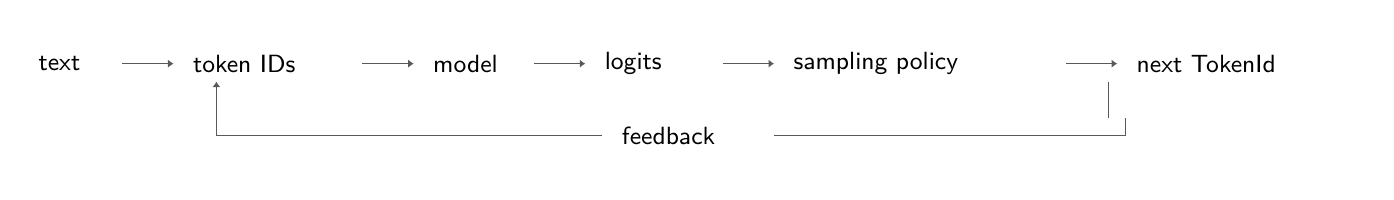
\begin{tikzpicture}[x=6.2pt,y=-13pt,draw=black!65,line width=.45pt]
\path[use as bounding box] (-1,-1) rectangle (77,3);
\draw (5,0) -- (4.5,0);
\draw (5,0) -- (5.5,0);
\draw (6,0) -- (5.5,0);
\draw (6,0) -- (6.5,0);
\draw[-{Latex[length=2pt,width=3pt]}] (6.5,0) -- (7.5,0);
\draw (19,0) -- (18.5,0);
\draw (19,0) -- (19.5,0);
\draw (20,0) -- (19.5,0);
\draw (20,0) -- (20.5,0);
\draw[-{Latex[length=2pt,width=3pt]}] (20.5,0) -- (21.5,0);
\draw (29,0) -- (28.5,0);
\draw (29,0) -- (29.5,0);
\draw (30,0) -- (29.5,0);
\draw (30,0) -- (30.5,0);
\draw[-{Latex[length=2pt,width=3pt]}] (30.5,0) -- (31.5,0);
\draw (40,0) -- (39.5,0);
\draw (40,0) -- (40.5,0);
\draw (41,0) -- (40.5,0);
\draw (41,0) -- (41.5,0);
\draw[-{Latex[length=2pt,width=3pt]}] (41.5,0) -- (42.5,0);
\draw (60,0) -- (59.5,0);
\draw (60,0) -- (60.5,0);
\draw (61,0) -- (60.5,0);
\draw (61,0) -- (61.5,0);
\draw[-{Latex[length=2pt,width=3pt]}] (61.5,0) -- (62.5,0);
\node[anchor=west,inner sep=0pt,font=\sffamily\fontsize{9}{11}\selectfont] at (-0.4,0) {\begin{adjustbox}{max width=24.8pt}text\end{adjustbox}};
\node[anchor=west,inner sep=0pt,font=\sffamily\fontsize{9}{11}\selectfont] at (8.6,0) {\begin{adjustbox}{max width=55.800000000000004pt}token IDs\end{adjustbox}};
\node[anchor=west,inner sep=0pt,font=\sffamily\fontsize{9}{11}\selectfont] at (22.6,0) {\begin{adjustbox}{max width=31.0pt}model\end{adjustbox}};
\node[anchor=west,inner sep=0pt,font=\sffamily\fontsize{9}{11}\selectfont] at (32.6,0) {\begin{adjustbox}{max width=37.2pt}logits\end{adjustbox}};
\node[anchor=west,inner sep=0pt,font=\sffamily\fontsize{9}{11}\selectfont] at (43.6,0) {\begin{adjustbox}{max width=93.0pt}sampling policy\end{adjustbox}};
\node[anchor=west,inner sep=0pt,font=\sffamily\fontsize{9}{11}\selectfont] at (63.6,0) {\begin{adjustbox}{max width=74.4pt}next TokenId\end{adjustbox}};
\draw[-{Latex[length=2pt,width=3pt]}] (10,1.5) -- (10,0.5);
\draw (62,1) -- (62,0.5);
\draw (62,1) -- (62,1.5);
\draw (10,2) -- (10.5,2);
\draw (10,2) -- (10,1.5);
\draw (11,2) -- (10.5,2);
\draw (11,2) -- (11.5,2);
\draw (12,2) -- (11.5,2);
\draw (12,2) -- (12.5,2);
\draw (13,2) -- (12.5,2);
\draw (13,2) -- (13.5,2);
\draw (14,2) -- (13.5,2);
\draw (14,2) -- (14.5,2);
\draw (15,2) -- (14.5,2);
\draw (15,2) -- (15.5,2);
\draw (16,2) -- (15.5,2);
\draw (16,2) -- (16.5,2);
\draw (17,2) -- (16.5,2);
\draw (17,2) -- (17.5,2);
\draw (18,2) -- (17.5,2);
\draw (18,2) -- (18.5,2);
\draw (19,2) -- (18.5,2);
\draw (19,2) -- (19.5,2);
\draw (20,2) -- (19.5,2);
\draw (20,2) -- (20.5,2);
\draw (21,2) -- (20.5,2);
\draw (21,2) -- (21.5,2);
\draw (22,2) -- (21.5,2);
\draw (22,2) -- (22.5,2);
\draw (23,2) -- (22.5,2);
\draw (23,2) -- (23.5,2);
\draw (24,2) -- (23.5,2);
\draw (24,2) -- (24.5,2);
\draw (25,2) -- (24.5,2);
\draw (25,2) -- (25.5,2);
\draw (26,2) -- (25.5,2);
\draw (26,2) -- (26.5,2);
\draw (27,2) -- (26.5,2);
\draw (27,2) -- (27.5,2);
\draw (28,2) -- (27.5,2);
\draw (28,2) -- (28.5,2);
\draw (29,2) -- (28.5,2);
\draw (29,2) -- (29.5,2);
\draw (30,2) -- (29.5,2);
\draw (30,2) -- (30.5,2);
\draw (31,2) -- (30.5,2);
\draw (31,2) -- (31.5,2);
\draw (32,2) -- (31.5,2);
\draw (32,2) -- (32.5,2);
\draw (43,2) -- (42.5,2);
\draw (43,2) -- (43.5,2);
\draw (44,2) -- (43.5,2);
\draw (44,2) -- (44.5,2);
\draw (45,2) -- (44.5,2);
\draw (45,2) -- (45.5,2);
\draw (46,2) -- (45.5,2);
\draw (46,2) -- (46.5,2);
\draw (47,2) -- (46.5,2);
\draw (47,2) -- (47.5,2);
\draw (48,2) -- (47.5,2);
\draw (48,2) -- (48.5,2);
\draw (49,2) -- (48.5,2);
\draw (49,2) -- (49.5,2);
\draw (50,2) -- (49.5,2);
\draw (50,2) -- (50.5,2);
\draw (51,2) -- (50.5,2);
\draw (51,2) -- (51.5,2);
\draw (52,2) -- (51.5,2);
\draw (52,2) -- (52.5,2);
\draw (53,2) -- (52.5,2);
\draw (53,2) -- (53.5,2);
\draw (54,2) -- (53.5,2);
\draw (54,2) -- (54.5,2);
\draw (55,2) -- (54.5,2);
\draw (55,2) -- (55.5,2);
\draw (56,2) -- (55.5,2);
\draw (56,2) -- (56.5,2);
\draw (57,2) -- (56.5,2);
\draw (57,2) -- (57.5,2);
\draw (58,2) -- (57.5,2);
\draw (58,2) -- (58.5,2);
\draw (59,2) -- (58.5,2);
\draw (59,2) -- (59.5,2);
\draw (60,2) -- (59.5,2);
\draw (60,2) -- (60.5,2);
\draw (61,2) -- (60.5,2);
\draw (61,2) -- (61.5,2);
\draw (62,2) -- (61.5,2);
\draw (62,2) -- (62.5,2);
\draw (63,2) -- (62.5,2);
\draw (63,2) -- (63,1.5);
\node[anchor=west,inner sep=0pt,font=\sffamily\fontsize{9}{11}\selectfont] at (33.6,2) {\begin{adjustbox}{max width=49.6pt}feedback\end{adjustbox}};
\end{tikzpicture}
\end{adjustbox}\end{center}

The result is small, but it is real. ENGINE-1 will support a separate
greedy path, numerically stable softmax, categorical sampling,
temperature, top-k, top-p, seeded request-local randomness, EOS,
output-token budgets, cancellation, failure, byte-safe streaming, and
exactly one terminal outcome. Nothing outside the model will manufacture
a candidate table. Every generated token will come from actual model
logits.

\subsection{The model has spoken---only in
numbers}\label{the-model-has-spokenonly-in-numbers}

A language model and an inference engine have different
responsibilities. The model maps token history to scores. The engine
decides how to use those scores, owns mutable generation state, returns
bytes, and stops the request.

\begin{quote}
\textbf{FIRST PRINCIPLE} The model predicts scores; the sampler chooses
an output token.
\end{quote}

Keeping this separation seems fussy in a four-token engine. It becomes
vital when one model serves concurrent requests with different sampling
policies, when a grammar masks candidates, when speculative decoding
verifies proposed tokens, or when an operator needs to compare raw model
output with the policy that transformed it.

ENGINE-1 therefore keeps this boundary:

\begin{verbatim}
Model::forward(&history) -> ForwardPass { logits, ... }
SamplerState::sample(&logits) -> SamplingStep { token_id, ... }
\end{verbatim}

\texttt{Logits} is evidence about what the model predicted. It is
finite, typed, and unchanged by sampling. A separate workspace holds
temperature-adjusted and filtered candidates.

\subsection{What autoregressive generation
means}\label{what-autoregressive-generation-means}

Suppose a token sequence contains random variables \(x_0,\ldots,x_T\).
The chain rule factors its joint probability:

\[
P(x_0,\ldots,x_T)
=\prod_{t=0}^{T}P\!\left(x_t\mid x_0,\ldots,x_{t-1}\right),
\]

where the \(t=0\) factor is the unconditional \(P(x_0)\).

An autoregressive language model repeatedly predicts the next token
given the tokens already visible. At step \texttt{t}, it produces scores
for \texttt{x\_(t+1)}. The engine chooses one candidate, appends that
token to the sequence, and runs the model again. Bengio and colleagues'
early \href{https://jmlr.org/papers/v3/bengio03a.html}{neural
probabilistic language model} is one primary source for this conditional
sequence framing.

The general statement is about full visible history. ENGINE-1 has a
deliberate limitation: its \texttt{\seqsplit{TinyLanguageModel}} reads
only \texttt{history.last()}. Two histories with the same final token
therefore produce identical logits, even if every earlier token differs.
ENGINE-1 implements genuine autoregressive feedback; its representation
is not yet context-sensitive.

That distinction matters. ``Autoregressive'' describes how outputs
become future inputs. It does not guarantee that a particular model uses
all history well---or at all.

\subsection{From logits to a probability
distribution}\label{from-logits-to-a-probability-distribution}

A logit is an unnormalized score. It may be negative, zero, or positive.
Its absolute value is not a probability, and the vector does not need to
sum to anything meaningful.

For a finite score vector
\(\mathbf{z}\in\mathbb{R}^{V_{\mathrm{vocab}}}\), softmax defines

\[
p_i=\frac{e^{z_i}}
{\sum_{j=0}^{V_{\mathrm{vocab}}-1}e^{z_j}},
\qquad
\mathbf{p}\in[0,1]^{V_{\mathrm{vocab}}},
\quad \sum_i p_i=1.
\]

Here:

\begin{itemize}
\tightlist
\item
  \(V_{\mathrm{vocab}}\) is vocabulary size;
\item
  \texttt{z\_i} is the raw score for token ID \texttt{i};
\item
  \texttt{p\_i} is that token's normalized probability;
\item
  \texttt{z} is \texttt{{[}V{]}} model output;
\item
  \texttt{p} is a \texttt{{[}V{]}} request-local distribution.
\end{itemize}

Every exponential is positive. The denominator is the sum of all
numerators. Therefore every \texttt{p\_i} is non-negative and the
probabilities sum to one in exact arithmetic. PyTorch's official
\href{https://docs.pytorch.org/docs/stable/generated/torch.nn.Softmax.html}{\texttt{Softmax}
documentation} states the same mathematical contract.

For logits \texttt{{[}1,2,3{]}}, the direct calculation is
approximately:

\begin{verbatim}
exp values = [2.718282, 7.389056, 20.085537]
sum        = 30.192875
p          = [0.090031, 0.244728, 0.665241]
\end{verbatim}

Token 2 remains the largest, but now the values describe a distribution
from which a categorical outcome can be drawn.

\subsubsection{Why naive softmax fails}\label{why-naive-softmax-fails}

Try logits \texttt{{[}1000,999,998{]}}. The ordering and gaps are
harmless. The direct implementation is not: \texttt{exp(1000)} overflows
ordinary floating-point storage. An infinite numerator can produce
infinite sums and undefined divisions.

The mathematical formula needs an equivalent numerical form. Let

\[
m=\max_{0\le j<V_{\mathrm{vocab}}}z_j,
\qquad
p_i=\frac{e^{z_i-m}}
{\sum_{j=0}^{V_{\mathrm{vocab}}-1}e^{z_j-m}}.
\]

Subtracting one constant from every score does not alter softmax. For
any finite constant \(c\):

\[
\frac{e^{z_i+c}}{\sum_j e^{z_j+c}}
=\frac{e^{z_i}e^c}{e^c\sum_j e^{z_j}}
=\frac{e^{z_i}}{\sum_j e^{z_j}}.
\]

With \texttt{c=-m}, every exponential argument is at most zero. At least
one is exactly zero, whose exponential is one. Numerators cannot
overflow, and the denominator cannot be zero.

This is \textbf{stable softmax}. Blanchard, Higham, and Higham analyze
shifted formulas in
\href{https://doi.org/10.1093/imanum/draa038}{Accurately computing the
log-sum-exp and softmax functions}. ENGINE-1 uses the clarity-first
maximum, exponential, sum, and normalization passes in \texttt{f64} for
the sampling workspace while preserving the model's raw \texttt{f32}
logits.

For \(\mathbf{z}=[1000,999,998]\), \(m=1000\) and

\[
\mathbf{z}-m=[0,-1,-2],\qquad
\mathbf{p}\approx[0.6652409558,0.2447284711,0.0900305732].
\]

The canonical
\href{https://github.com/hermonai/inside-the-llm-engine/blob/astra-visual-rewrite/diagrams/sampling/stable-softmax.txt}{stable-softmax
flow} connects these equations to the implementation passes.

All results are finite.

\begin{quote}
\textbf{ENGINEERING FAILURE --- NAIVE SOFTMAX} A mathematically
recognizable expression can still be an invalid numerical program.
Algebraic equivalence does not imply equal floating-point behavior.
\end{quote}

\subsection{Greedy decoding needs no
softmax}\label{greedy-decoding-needs-no-softmax}

Softmax preserves ordering because exponentiation is strictly increasing
and every candidate shares the same positive denominator:

\[
\operatorname*{arg\,max}_i z_i
=\operatorname*{arg\,max}_i \operatorname{softmax}(\mathbf{z})_i.
\]

Greedy decoding can scan raw logits and choose the maximum. It does not
need exponentials or normalized probabilities.

ENGINE-1 treats greedy as a separate
\texttt{\seqsplit{SamplingConfig::Greedy}} mode. It never divides by
temperature zero and does not approximate greedy with a tiny positive
temperature. A strict \texttt{\textgreater{}} comparison replaces the
current winner; iteration proceeds in token-ID order. Equal maxima
therefore choose the lowest token ID, deliberately and reproducibly.

Greedy is deterministic and inexpensive: one \texttt{O(V)} scan. It is
not globally optimal sequence search. Choosing the locally highest
next-token score does not prove that the resulting complete sequence has
the greatest joint probability. Greedy can also produce dull or
repetitive text. Those are policy tradeoffs, not reasons to hide its
simple semantics.

\subsection{Randomness is request
state}\label{randomness-is-request-state}

Random sampling is not a command sent to the model. It is stateful
computation in the engine.

\begin{verbatim}
REQUEST
  prompt and generated history
  immutable sampler configuration
  mutable PRNG state
  successful sample count
  remaining output budget
  terminal state
\end{verbatim}

A pseudorandom number generator, or PRNG, advances deterministic
internal state. A seed chooses its starting state. Give the same
algorithm the same seed and consume values in the same order, and it
produces the same number sequence.

ENGINE-1 implements SplitMix64, derived from the design described by
Steele, Lea, and Flood in
\href{https://doi.org/10.1145/2660193.2660195}{Fast Splittable
Pseudorandom Number Generators}. It uses wrapping \texttt{u64}
arithmetic and converts the high 53 output bits into a binary64 draw in
\texttt{{[}0,1)}.

This generator is compact, deterministic, and testable. It is not
cryptographically secure, and the engine never describes it that way.

Each admitted request constructs a fresh \texttt{SamplerState}. Two
concurrent requests do not share one mutable RNG. Otherwise scheduling
would change which request consumes which draw:

\begin{verbatim}
global draws: r0 r1 r2 r3 ...

schedule A,B,A,B -> A gets r0,r2; B gets r1,r3
schedule A,A,B,B -> A gets r0,r1; B gets r2,r3
\end{verbatim}

The model and seeds could be identical while outputs changed with
scheduling. Per-request state removes that coupling.

\begin{quote}
\textbf{FIRST PRINCIPLE} Randomness is mutable request state, not a
hidden global service.
\end{quote}

\subsubsection{What a seed guarantees}\label{what-a-seed-guarantees}

ENGINE-1's promise is intentionally bounded:

\begin{quote}
For the same ENGINE-1 commit, executable/toolchain/target, model
parameters, tokenizer, prompt tokens, sampling configuration, and seed,
the scalar path repeats the same token sequence.
\end{quote}

A fixed seed alone does not guarantee identical output across engine
versions, models, providers, quantizations, RNG algorithms,
floating-point libraries, or sampler orders. Even tiny logit or
cumulative-boundary changes can map a draw to another token.

``Seed equals determinism everywhere'' is therefore false. A seed is one
member of a reproduction contract.

\subsection{Categorical sampling, one interval at a
time}\label{categorical-sampling-one-interval-at-a-time}

Suppose \(\mathbf{p}=[0.20,0.30,0.50]\). Define cumulative boundaries
\(c_i=\sum_{j=0}^{i}p_j\) and \(c_{-1}=0\). For a draw \(r\sim U[0,1)\),
select

\[
i=\min\{k:r<c_k\},
\qquad\text{equivalently}\qquad c_{i-1}\le r<c_i.
\]

Their cumulative boundaries divide \texttt{{[}0,1)}:

\begin{verbatim}
0.0                 0.2                         0.5                    1.0
 |------ token 0 -----|----------- token 1 -------|------- token 2 -----|
\end{verbatim}

Draw \texttt{r} uniformly in \texttt{{[}0,1)}. Select the first
cumulative boundary strictly greater than \texttt{r}:

\begin{verbatim}
r=0.19 -> token 0
r=0.20 -> token 1
r=0.49 -> token 1
r=0.50 -> token 2
r=0.99 -> token 2
\end{verbatim}

ENGINE-1 exposes the pure boundary as:

\begin{verbatim}
categorical_select(probabilities, draw) -> Result<TokenId, SamplingError>
\end{verbatim}

The RNG is only one producer of \texttt{draw}. Tests and the independent
Python oracle can supply an artificial value. This separation prevents
one failing test from becoming an unsolved mixture of softmax,
filtering, PRNG, and cumulative-selection bugs.

The function validates finite, non-negative probabilities and a sum
within tolerance of one. Floating-point rounding can leave the last
cumulative sum a few ulps below one. If a valid draw survives every
earlier interval, the implementation returns the final
positive-probability candidate. It never uses that fallback to rescue an
invalid or empty distribution.

\subsection{Temperature changes shape, not
randomness}\label{temperature-changes-shape-not-randomness}

For stochastic mode, ENGINE-1 requires a finite temperature \(\tau>0\)
and transforms scores:

\[
z'_i=\frac{z_i}{\tau}.
\]

Then it computes the distribution. Temperature affects score gaps:

\begin{itemize}
\tightlist
\item
  \(\tau<1\) magnifies gaps and sharpens the distribution;
\item
  \(\tau=1\) leaves scores unchanged;
\item
  \(\tau>1\) shrinks gaps and flattens the distribution.
\end{itemize}

Positive division preserves ordering. For logits \texttt{{[}1,2,3{]}}:

{\def\LTcaptype{none} % do not increment counter
\begin{longtable}[]{@{}rl@{}}
\toprule\noalign{}
Temperature & Probabilities \\
\midrule\noalign{}
\endhead
\bottomrule\noalign{}
\endlastfoot
0.5 & \texttt{\seqsplit{[0.015876,0.117310,0.866813]}} \\
1.0 & \texttt{\seqsplit{[0.090031,0.244728,0.665241]}} \\
2.0 & \texttt{\seqsplit{[0.186324,0.307196,0.506480]}} \\
\end{longtable}
}

Token 2 stays highest. The cold distribution concentrates more mass on
it; the hot distribution spreads more mass to alternatives.

Temperature does not produce a draw. If selection remains greedy,
changing a positive temperature cannot change the winner. Randomness
comes from categorical sampling.

ENGINE-1 rejects zero, negative, NaN, and infinite stochastic
temperatures. Greedy remains a different mode. This makes the API say
what it means.

\subsection{Top-k: a fixed candidate
count}\label{top-k-a-fixed-candidate-count}

A production vocabulary may contain tens of thousands of candidates.
Many receive tiny probability. Top-k keeps the \texttt{k} highest scores
and removes the rest before sampling:

\begin{verbatim}
scores -> order/select highest k -> mask others -> normalize -> sample
\end{verbatim}

Because softmax preserves ordering, ENGINE-1 applies top-k in logit
space. Its simple teaching implementation sorts indexes by score
descending and token ID ascending. It stores removed entries as
\texttt{None} in a workspace rather than putting negative infinity into
raw \texttt{Logits}.

The edge contract is explicit:

\begin{itemize}
\tightlist
\item
  \texttt{None}: disabled;
\item
  \texttt{k=0}: invalid;
\item
  \texttt{k=1}: one survivor, hence probability one;
\item
  \texttt{k\textgreater{}=V}: no filtering.
\end{itemize}

Sorting costs \texttt{O(V\ log\ V)} in this implementation. A production
sampler may use partial selection, but optimization would not change the
survivor semantics or deterministic tie rule.

\subsection{Top-p: an adaptive probability
mass}\label{top-p-an-adaptive-probability-mass}

Top-p, or nucleus sampling, keeps a variable-size set. Sort candidates
by probability descending and retain the smallest prefix whose
cumulative mass reaches threshold \texttt{p}. Holtzman and colleagues
introduced and evaluated this policy in
\href{https://arxiv.org/abs/1904.09751}{The Curious Case of Neural Text
Degeneration}.

Consider:

{\def\LTcaptype{none} % do not increment counter
\begin{longtable}[]{@{}lr@{}}
\toprule\noalign{}
Token & Probability \\
\midrule\noalign{}
\endhead
\bottomrule\noalign{}
\endlastfoot
A & 0.40 \\
B & 0.30 \\
C & 0.15 \\
D & 0.10 \\
E & 0.05 \\
\end{longtable}
}

For threshold \(\tau_p=0.80\), A and B provide only \(0.70\). C crosses
the threshold, so C is included. The nucleus is A/B/C with mass
\texttt{0.85}. ENGINE-1 renormalizes:

\begin{verbatim}
[0.470588,0.352941,0.176471,0,0]
\end{verbatim}

Top-k retains a fixed count. Top-p retains an adaptive count determined
by the distribution's concentration. Neither is universally superior.

Formally, after sorting
\(p_{(0)}\ge\cdots\ge p_{(V_{\mathrm{vocab}}-1)}\), the retained prefix
ends at

\[
m=\min\left\{k:\sum_{j=0}^{k}p_{(j)}\ge\tau_p\right\}.
\]

ENGINE-1 accepts \(\tau_p\) only in \((0,1]\); \(\tau_p=1\) is a
deliberate no-op. Equal probabilities use token ID ascending as the
secondary order.

\subsection{Filter order is inference
behavior}\label{filter-order-is-inference-behavior}

Temperature, top-k, and top-p are not a bag of commutative options.
Their order can change the candidate set and final probabilities.

ENGINE-1 fixes this pipeline:

\begin{verbatim}
raw finite logits
  -> copy and divide by temperature
  -> top-k mask in logit space
  -> stable softmax over survivors
  -> top-p filter in probability space
  -> renormalize
  -> categorical draw
\end{verbatim}

The implementation and prose use this exact order. Configuration fields
do not silently determine order.

Other engines can choose differently. In particular, the current Hermon
shim examined later builds a llama.cpp-backed chain with a different
order. That is not a contradiction. Sampling order is policy, and
reproducibility requires identifying the policy.

\href{https://github.com/hermonai/inside-the-llm-engine/blob/astra-visual-rewrite/diagrams/sampling/sampling-pipeline.txt}{The
canonical sampling pipeline} keeps raw logits separate from processed
candidates.

\begin{quote}
\textbf{ENGINEERING FAILURE --- DESTROYED EVIDENCE} If top-k mutates raw
logits in place, a later debugger sees masks rather than model output.
Keep the model prediction and the sampler decision as separate
artifacts.
\end{quote}

\subsection{The complete ENGINE-1
loop}\label{the-complete-engine-1-loop}

The runtime's operation order now has a precise commit point:

\begin{enumerate}
\def\labelenumi{\arabic{enumi}.}
\tightlist
\item
  Validate input tokens, \texttt{max\_new\_tokens}, and sampling
  configuration.
\item
  Construct a fresh request-owned \texttt{SamplerState}.
\item
  Admit the request and begin execution.
\item
  Check cancellation and output budget.
\item
  Build history from prompt plus committed output tokens.
\item
  Run \texttt{Model::forward} and validate exactly \texttt{V} logits.
\item
  Preserve and optionally trace the raw forward result.
\item
  Check cancellation again before sampling.
\item
  Select a \texttt{TokenId}; trace probabilities and draw for stochastic
  mode.
\item
  If it is EOS, stop without decoding or streaming it.
\item
  Otherwise append it to \texttt{GenerationState}. This is the commit
  point.
\item
  Emit token identity, decode bytes, frame strict UTF-8, and emit text.
\item
  Repeat or transition exactly once to terminal state.
\end{enumerate}

The
\href{https://github.com/hermonai/inside-the-llm-engine/blob/astra-visual-rewrite/diagrams/sampling/autoregressive-state.txt}{autoregressive
state diagram} distinguishes data movement from stop checks.

\subsubsection{A complete greedy trace}\label{a-complete-greedy-trace}

Prompt text:

\begin{verbatim}
I like
\end{verbatim}

Tokenizer output:

\begin{verbatim}
[1,2]
\end{verbatim}

The last token is \texttt{like}. Chapter 3 computed:

\begin{verbatim}
hidden = [1,-0.5,2]
logits = [-0.7,0.1,0.4,2.2]
argmax = 3 = Rust
\end{verbatim}

The runtime appends token 3:

\begin{verbatim}
[1,2,3]
\end{verbatim}

It decodes token 3 to the byte piece for \texttt{Rust}, emits valid
text, and runs the model again. ENGINE-1 reads the final \texttt{Rust}
token:

\begin{verbatim}
hidden = [-1,0,0]
logits = [0.3,-0.2,-0.3,-0.5]
argmax = 0 = <eos>
\end{verbatim}

EOS completes the request. It is not added to visible output, decoded,
or streamed. The complete model-derived path is:

\begin{verbatim}
"I like" -> [1,2] -> Rust -> [1,2,3] -> <eos> -> completed
\end{verbatim}

No fake candidate table produces \texttt{Rust}.

\subsubsection{A seeded stochastic
trace}\label{a-seeded-stochastic-trace}

Run:

\begin{verbatim}
cd code/mini-engine
cargo run -p engine0 -- --trace --sample --temperature 1 \
  --top-k 3 --top-p .9 --seed 42 --max-tokens 3 'I like'
\end{verbatim}

At the first step, ENGINE-1 records raw logits, then:

\begin{verbatim}
probabilities = [0,0,0.1418510634,0.8581489366]
draw          = 0.7415648788
selected      = 3
\end{verbatim}

At the next step:

\begin{verbatim}
probabilities = [0.4639634327,0.2814080427,0.2546285245,0]
draw          = 0.1599103929
selected      = 0 = <eos>
\end{verbatim}

The same bounded reproduction environment repeats those draws and
tokens. Timing fields are not part of semantic equality.

\subsection{EOS, budgets, and visible
output}\label{eos-budgets-and-visible-output}

EOS is a vocabulary token with a model score. It is also semantic
control. ENGINE-1 chooses this policy:

\begin{itemize}
\tightlist
\item
  sampled EOS ends generation;
\item
  EOS is not committed to the visible generated-token list;
\item
  EOS is not decoded to bytes;
\item
  EOS is not streamed as ordinary text;
\item
  terminal reason is \texttt{EndOfSequence}.
\end{itemize}

\texttt{max\_new\_tokens} counts committed non-EOS output tokens. A
prompt of ten tokens and \texttt{\seqsplit{max\_new\_tokens=5}} allows
at most five new visible tokens; it does not cap the total sequence at
five.

Application stop strings are more complicated. A string can span tokens
and UTF-8 pieces, and policy must decide whether matching bytes are
included or removed. Chapter 4 defers that design. Its core stop set is
EOS, output budget, cancellation, and failure.

\subsection{Cancellation and failure without partial
ambiguity}\label{cancellation-and-failure-without-partial-ambiguity}

Cancellation is checked before a forward and again after forward before
sampling. If cancellation is observed at either point, no later token is
committed. The current engine is synchronous, but this placement
establishes the invariant an asynchronous runtime must preserve.

Sampling can fail. Invalid temperature, top-k, or top-p does not
silently fall back to greedy. Empty logits, non-finite processed values,
negative probabilities, invalid sums, invalid draws, and empty candidate
sets have typed errors.

For a non-EOS token, ENGINE-1 commits it before tokenizer/UTF-8
processing. If decoding fails afterward, the generation result contains
the committed token and a failed terminal outcome. This is more truthful
than pretending the model never selected it. Stream consumers may
already have received token identity, so rollback would be dishonest
without a richer transactional protocol.

Terminal delivery still has one owner:
\texttt{\seqsplit{Lifecycle::finish}}. Every successful, cancelled, or
failed branch returns an outcome to that owner. It emits one terminal
stream event, records one terminal trace event, and closes future
emission. A second transition returns \texttt{AlreadyTerminal}.

\begin{quote}
\textbf{ENGINEERING FAILURE --- DOUBLE TERMINATION} If the EOS branch
emits \texttt{Done} and loop cleanup emits another \texttt{Done}, the
client sees two endings. Terminal success is a state transition, not an
informal callback.
\end{quote}

\begin{quote}
\textbf{ENGINEERING FAILURE --- POST-EOS OUTPUT} If the loop appends or
decodes another token before checking EOS, its sequence and stream
disagree with model control. Stop ordering must be explicit.
\end{quote}

\subsection{Follow the token, byte, and
owner}\label{follow-the-token-byte-and-owner-1}

Part I can now complete all three recurring journeys.

\subsubsection{Follow the token}\label{follow-the-token-1}

\begin{verbatim}
human text
 -> tokenizer
 -> TokenId history
 -> embedding row
 -> hidden activation
 -> output projection
 -> raw logits
 -> temperature/filtering
 -> greedy or categorical selection
 -> new TokenId
 -> append
 -> model again
\end{verbatim}

The reusable
\href{https://github.com/hermonai/inside-the-llm-engine/blob/astra-visual-rewrite/diagrams/sampling/part1-follow-token.txt}{Part
I token diagram} also shows the decode and stream branch.

\subsubsection{Follow the byte}\label{follow-the-byte-1}

Model parameter bytes are read by scalar \texttt{f32} arithmetic. The
result is a finite raw \texttt{f32} logit vector. Stochastic processing
copies values to a request-local \texttt{f64} workspace. Selection
yields an integer token ID. The tokenizer maps that ID to bytes, the
UTF-8 decoder holds incomplete suffixes, and only valid complete text
reaches the stream.

See
\href{https://github.com/hermonai/inside-the-llm-engine/blob/astra-visual-rewrite/diagrams/sampling/part1-follow-byte.txt}{Part
I follow the byte}.

\subsubsection{Follow the owner}\label{follow-the-owner-1}

The model lifetime owns immutable parameters and the tokenizer/model
contract. A request owns prompt tokens, committed output, sampling
configuration, RNG state, budget, UTF-8 buffer, and terminal state. A
forward step owns temporary hidden values, raw logits, processed
candidates, and one selection.

See
\href{https://github.com/hermonai/inside-the-llm-engine/blob/astra-visual-rewrite/diagrams/sampling/part1-follow-owner.txt}{Part
I follow the owner}.

This separation prepares the engine for concurrency:

\begin{verbatim}
                         shared MODEL
                      immutable weights
                       /             \
              Request A               Request B
             history/RNG A           history/RNG B
\end{verbatim}

The model can be shared. Mutable sequence and sampler state cannot. A
future continuous batch may evaluate several sequences together, but
sampling remains logically per sequence. The
\href{https://github.com/hermonai/inside-the-llm-engine/blob/astra-visual-rewrite/diagrams/sampling/model-two-requests.txt}{two-request
ownership diagram} makes that future constraint visible.

\subsection{Build it: the sampler and
runtime}\label{build-it-the-sampler-and-runtime}

The Chapter 4 implementation lives in:

\begin{verbatim}
code/mini-engine/crates/engine0/src/sampling.rs
code/mini-engine/crates/engine0/src/lib.rs
\end{verbatim}

The public design separates immutable and mutable pieces:

\begin{verbatim}
SamplingConfig       // mode and parameters, carried by Request
SamplerState         // one RNG and sample count per generate call
ProbabilityDistribution
SamplingStep         // token, optional probabilities/draw, sample index
SamplingError        // typed validation and numerical failures
\end{verbatim}

The model still returns \texttt{Logits}. It has no RNG, no temperature,
and no stop policy. The runtime no longer carries the old temporary
\texttt{GreedySelector}. Instead it creates a sampler from each
request's configuration.

Trace mode exposes tiny educational fixtures:

\begin{verbatim}
[model] raw logits
[sampler] immutable configuration
[sampler] processed probabilities, when stochastic
[sampler] request-local draw, when stochastic
[sampler] selected TokenId
[sequence] commit non-EOS token
[tokenizer/stream] bytes and valid text
\end{verbatim}

Production tracing should not log sensitive prompts or huge tensors by
default. ENGINE-1's \texttt{TraceSink} already requires an explicit
opt-in for full values.

\subsection{Prove it: an independent
oracle}\label{prove-it-an-independent-oracle}

\texttt{\seqsplit{code/reference/python/chapter04\_sampling\_oracle.py}}
independently implements stable softmax, temperature, top-k, top-p,
renormalization, and fixed-draw categorical selection. It imports no
Rust engine code.

Run:

\begin{verbatim}
python3 code/reference/python/chapter04_sampling_oracle.py \
  --logits -0.7 0.1 0.4 2.2 \
  --temperature 1 --top-k 3 --top-p .9 --draw .63
\end{verbatim}

Expected core output:

\begin{verbatim}
probabilities = [0,0,0.1418510649,0.8581489351]
retained      = [2,3]
selected      = 3
PASS
\end{verbatim}

The fixed draw is important. A numerical oracle should not need to
duplicate ENGINE-1's PRNG before it can prove the cumulative boundary.
RNG output vectors are tested separately.

Rust tests cover 83 cases across the workspace. Twenty dedicated
sampling tests cover numerical values, large-logit stability, shift
invariance, probability invariants, greedy ties, temperature,
top-k/top-p edges and order, fixed draws, pinned SplitMix64 output,
same/different seeds, raw-logit preservation, and a deterministic
property grid. Lifecycle tests cover EOS, budget, cancellation at both
checkpoints, model/sampler/tokenizer/UTF-8 failure, per-request seed
isolation, no post-terminal output, and exactly one terminal event.

\begin{quote}
\textbf{PROVE IT} A sampler is correct only when its stages can be
checked independently and its full loop preserves lifecycle invariants.
\end{quote}

\subsection{Performance lab: sampling is
work}\label{performance-lab-sampling-is-work}

Sampling over vocabulary size \texttt{V} can require:

\begin{itemize}
\tightlist
\item
  a maximum scan;
\item
  temperature scaling;
\item
  exponentiation and summation;
\item
  sorting or selection for filters;
\item
  renormalization;
\item
  a cumulative scan.
\end{itemize}

Greedy needs only the maximum scan. ENGINE-1's teaching top-k and top-p
use straightforward sorting for clarity. Their asymptotic and constant
costs are visible.

The reproducible probe in
\texttt{\seqsplit{code/mini-engine/crates/engine0/examples/chapter04\_sampling\_cost.rs}}
measures sampling separately from model forward on an Apple M1. The full
record is
\href{https://github.com/hermonai/inside-the-llm-engine/blob/astra-visual-rewrite/research/benchmarks/chapter-04-sampling-cost.md}{\texttt{\seqsplit{research/benchmarks/chapter-04-sampling-cost.md}}}.

Exploratory medians in nanoseconds per call were:

{\def\LTcaptype{none} % do not increment counter
\begin{longtable}[]{@{}rrrrr@{}}
\toprule\noalign{}
V & Greedy & Softmax + categorical & Top-k 40 & Top-p .9 \\
\midrule\noalign{}
\endhead
\bottomrule\noalign{}
\endlastfoot
16 & 26 & 341 & 472 & 597 \\
256 & 284 & 2,832 & 5,295 & 6,817 \\
4,096 & 5,137 & 41,467 & 107,582 & 127,452 \\
\end{longtable}
}

These numbers are not end-to-end token latency and cannot be
extrapolated to production models. They exclude the model entirely. They
show only that the extra passes and clarity-first sorting have
measurable cost in ENGINE-1. For large language models, forward
execution is often much more expensive, but that proportion depends on
model, hardware, provider, vocabulary, batching, and implementation.
Measure the actual system before making a latency claim.

\subsection{Inside Hermon}\label{inside-hermon}

Hermon is the production case study, not the teaching implementation.
The following behavior was inspected at commit
\texttt{\seqsplit{472a44cdb511b2dae6c9569e59543db8f8350b25}}; its
llama.cpp submodule was pinned at
\texttt{\seqsplit{389ff61d77b5c71cec0cf92fe4e5d01ace80b797}}.

\begin{quote}
\textbf{INSIDE HERMON --- CURRENT} The default batched runtime carries
sampler configuration in each submitted request and constructs one
mutable llama.cpp sampler for each \texttt{ActiveSeq}. Model work may be
batched, but eligible logit rows are sampled through their owning
sequences' sampler objects.
\end{quote}

\texttt{\seqsplit{crates/hermon-runtime/src/batched.rs}} stores prompt
tokens, pending token, completion count, maximum completion count, UTF-8
buffer, generated history, and concrete sampler in \texttt{ActiveSeq}.
Admission constructs that sampler. The worker requests logits for
eligible sequence positions, samples per sequence, checks
end-of-generation and budget, updates pending state, streams pieces, and
eventually sends \texttt{\seqsplit{StreamItem::Done(EngineMetrics)}}.
Error branches send an error rather than \texttt{Done}.

The linked facade in
\texttt{\seqsplit{crates/hermon-llamacpp/src/linked.rs}} owns a native
\texttt{llama\_sampler*}. Sampling takes mutable sampler and context
references plus the relevant logit-row index. The simpler iterator path
makes the feedback loop visible: sample from the previous decode, stop
on EOG, feed the selected token through decode so KV state advances,
decrement remaining budget, and return the token.

Hermon's C shim at this commit chooses a greedy llama.cpp sampler when
\texttt{temperature\textless{}=0}. Otherwise it constructs top-k → top-p
→ min-p → temperature → distribution. Seed zero becomes time-derived in
the shim. That chain is Hermon's current wrapper policy; it is not
ENGINE-1's order.

\begin{quote}
\textbf{INSIDE HERMON --- PREVIEW} The gated Hermon-owned paged GGUF
runtime is still CPU and greedy-only. Its source uses local argmax in
the paged loop, and the documented 1,000-prompt temperature-zero
equivalence corpus remains a release gate.
\end{quote}

This status distinction prevents two misleading claims: the existence of
stochastic sampling on Hermon's default llama.cpp-backed path does not
mean the Hermon-owned paged path supports it, and an implemented paged
path does not mean it is the default release path.

\subsubsection{The pinned llama.cpp
library}\label{the-pinned-llama.cpp-library}

The pinned public \texttt{llama.h} documents sampler chains ending in a
selection stage such as greedy or distribution. Its current CPU greedy
implementation uses a strict greater-than scan. Its distribution sampler
owns seeded \texttt{std::mt19937} state, performs a maximum-shifted
exponential computation, and draws cumulatively. Top-k truncates
score-ordered candidates; top-p computes probabilities, orders them, and
includes the threshold-crossing candidate.

ENGINE-1 borrows none of that code and promises no RNG identity with it.
The comparison validates boundaries: logits exist before selection,
sampler state is mutable, chain order matters, and end-of-generation
belongs to the runtime.

\subsection{Why raw logits are durable
evidence}\label{why-raw-logits-are-durable-evidence}

It is tempting to treat a logit vector as disposable scratch. After all,
the request needs only one token. That shortcut destroys information at
exactly the boundary where inference behavior is hardest to debug.

Suppose a user reports that token 17 appeared unexpectedly. Several
different causes can lead there:

\begin{itemize}
\tightlist
\item
  the model genuinely assigned token 17 a large raw score;
\item
  temperature flattened a concentrated distribution;
\item
  top-k removed a token that would otherwise dominate;
\item
  top-p's retained set changed at a cumulative boundary;
\item
  a grammar or future constraint masked alternatives;
\item
  the RNG draw landed in token 17's interval;
\item
  token IDs and tokenizer bytes did not match the intended model
  revision.
\end{itemize}

If the sampler overwrote raw logits, these explanations collapse into
one processed vector. If trace data retains raw logits, processed
probabilities, configuration, draw, and selected ID as distinct
artifacts, each stage can be audited.

This is also a correctness requirement for future speculative decoding.
A draft model may propose several tokens, but a target model must verify
them under the target sampling semantics. Constrained generation may add
grammar, JSON-schema, tool-syntax, repetition, or forbidden-token masks.
Those processors answer ``which outputs are currently allowed?'' Raw
logits answer ``what did the model predict before policy?'' The
questions are related but not identical.

ENGINE-1 does not implement those future processors. It establishes the
seam they require:

\begin{verbatim}
raw model evidence -> ordered logit processors -> candidate distribution
                   -> stateful selection -> committed token
\end{verbatim}

\begin{quote}
\textbf{FIRST PRINCIPLE} Sampling policy is inference behavior, not
model weights. Preserve the evidence on both sides of that policy
boundary.
\end{quote}

\subsection{Renormalization is not
optional}\label{renormalization-is-not-optional}

Softmax initially distributes one unit of mass over active candidates.
Top-p then removes some candidates. If the retained probabilities sum to
\texttt{0.85}, sampling directly against intervals ending at
\texttt{0.85} leaves \texttt{{[}0.85,1)} without a mathematically owned
token.

One could scale a random draw by retained mass, but that is
renormalization in another form. ENGINE-1 performs it explicitly:

\[
q_i=
\begin{cases}
\displaystyle\frac{p_i}{\sum_{j\in S}p_j}, & i\in S,\\[6pt]
0, & i\notin S,
\end{cases}
\]

where \(S\) is the retained candidate set.

Now retained \texttt{q\_i} values sum approximately to one. The
categorical selector has one contract regardless of which filters ran.
Stage tests compose cleanly: distribution construction proves
normalization, and categorical selection assumes normalized input.

The distinction clarifies the all-filtered failure. If candidate mass is
zero, there is no denominator and no distribution. ENGINE-1 returns
\texttt{\seqsplit{AllCandidatesFiltered}}; it does not unmask a
convenient token or switch to greedy. A future policy may require
``always keep at least one,'' but that rule must be explicit in the
processor that owns it.

\subsection{A lifecycle matrix for the real
loop}\label{a-lifecycle-matrix-for-the-real-loop}

The canonical
\href{https://github.com/hermonai/inside-the-llm-engine/blob/astra-visual-rewrite/diagrams/sampling/generation-terminal-state-machine.txt}{generation
state machine} makes the transition events and three terminal states
explicit.

The happy path alone cannot establish runtime correctness. Consider what
has been committed and what may be emitted at each terminal cause:

{\def\LTcaptype{none} % do not increment counter
\begin{longtable}[]{@{}
  >{\raggedright\arraybackslash}p{(\linewidth - 8\tabcolsep) * \real{0.2000}}
  >{\raggedright\arraybackslash}p{(\linewidth - 8\tabcolsep) * \real{0.2000}}
  >{\raggedright\arraybackslash}p{(\linewidth - 8\tabcolsep) * \real{0.2000}}
  >{\raggedright\arraybackslash}p{(\linewidth - 8\tabcolsep) * \real{0.2000}}
  >{\raggedright\arraybackslash}p{(\linewidth - 8\tabcolsep) * \real{0.2000}}@{}}
\toprule\noalign{}
\begin{minipage}[b]{\linewidth}\raggedright
Cause
\end{minipage} & \begin{minipage}[b]{\linewidth}\raggedright
Token selected?
\end{minipage} & \begin{minipage}[b]{\linewidth}\raggedright
Token committed?
\end{minipage} & \begin{minipage}[b]{\linewidth}\raggedright
Text emitted?
\end{minipage} & \begin{minipage}[b]{\linewidth}\raggedright
Terminal
\end{minipage} \\
\midrule\noalign{}
\endhead
\bottomrule\noalign{}
\endlastfoot
EOS & yes, EOS & no & no EOS text & completed: EOS \\
Budget before next step & previous only & previous only & previous text
& completed: max tokens \\
Cancel before forward & no new token & no & no & cancelled \\
Cancel after forward & no new sample & no & no & cancelled \\
Model failure & no & no & no new text & failed: model \\
Sampling failure & no token & no & no new text & failed: sampling \\
Tokenizer failure & yes, non-EOS & yes & token event may exist & failed:
tokenizer \\
UTF-8 failure & yes, non-EOS & yes & only prior valid text & failed:
UTF-8 \\
\end{longtable}
}

The table exposes why ``stop the loop'' is insufficient as a design. A
stop has a point in the state transition. An EOS decision occurs before
commit. Tokenizer failure occurs after commit. Cancellation can occur on
either side of expensive model work but before selection. The result
must reflect those facts.

ENGINE-1's stream is ordered:

\begin{verbatim}
zero or more token/text events -> exactly one Terminal event -> nothing
\end{verbatim}

Text events need not correspond one-to-one with token events because a
token piece may end in an incomplete UTF-8 scalar. The decoder buffers
bytes until a valid prefix exists. Sampling is token-level; user-visible
streaming is byte/text-level. Chapter 2's boundary remains active inside
Chapter 4's loop.

\subsection{Selection state under future
batching}\label{selection-state-under-future-batching}

Continuous batching will eventually assemble model work from several
sequences:

\begin{verbatim}
Request A tokens --+
Request B tokens ---+--> model batch --> logits A, logits B, logits C
Request C tokens --+
\end{verbatim}

That physical batch does not merge logical sequences. Row A must be
processed with A's configuration, RNG state, token history, and
remaining budget. A worker may change the order in which sequences enter
batches without changing which RNG stream each sequence consumes.

This is why request-owned randomness is a systems rule, not a detail of
random number generation. State ownership makes scheduling freedom
possible. A global RNG would turn an optimization---reordering batch
work---into a semantic change.

Speculative decoding creates another version of the same constraint. A
draft path may propose multiple candidates in one step, but accepted
output still has to obey the target model and chosen sampling contract.
Rollback must restore model/KV state and stateful processors
consistently. Chapter 4 does not implement speculation; it supplies the
raw-logit, sampler-state, and commit boundaries later chapters will
need.

\subsection{Seven first principles,
connected}\label{seven-first-principles-connected}

The chapter's individual rules form one chain:

\begin{enumerate}
\def\labelenumi{\arabic{enumi}.}
\tightlist
\item
  \textbf{The model predicts scores; the sampler chooses a token.} This
  separates learned model semantics from request policy.
\item
  \textbf{Equivalent mathematics can have different numerical safety.}
  Stable softmax preserves semantics while preventing exponential
  overflow.
\item
  \textbf{Randomness is owned mutable state.} Seeds and consumption
  order belong to one request.
\item
  \textbf{Sampling policy is part of inference behavior.} Temperature,
  filters, tie rules, order, and RNG algorithm belong in a reproduction
  record.
\item
  \textbf{Raw and processed scores are different artifacts.} Debugging
  and future constraints need both.
\item
  \textbf{Selected output becomes future input.} Feedback is the
  operational heart of autoregressive generation.
\item
  \textbf{Termination has one owner and defined commit points.} EOS,
  budget, cancellation, and failure must produce one coherent final
  outcome.
\end{enumerate}

Remove any one rule and the tiny engine develops a production-shaped
bug. Put softmax inside the model, and sampling policy contaminates
model semantics. Use naive exponentials, and ordinary logits can yield
NaNs. Share an RNG, and scheduling changes text. Mutate raw scores, and
debugging loses evidence. Append before checking EOS, and sequence state
lies. Emit terminal events in several branches, and clients can receive
contradictory endings.

That is why ENGINE-1 spends more code on contracts and tests than on the
few lines of exponential arithmetic. The arithmetic chooses a token; the
contracts make that choice meaningful inside a system.

\subsection{Common mistakes}\label{common-mistakes-3}

\subsubsection{``Logits are
probabilities''}\label{logits-are-probabilities}

Logits are unnormalized scores. They can be negative and do not sum to
one. Softmax creates probabilities when a policy needs them.

\subsubsection{``Softmax belongs in every
forward''}\label{softmax-belongs-in-every-forward}

The model boundary returns logits. Greedy can consume them directly;
other processors may need raw scores. Making softmax mandatory would
conflate model semantics with selection policy.

\subsubsection{``The highest logit must be
selected''}\label{the-highest-logit-must-be-selected}

Greedy selects it. Categorical sampling can choose any
positive-probability candidate retained by policy.

\subsubsection{``Temperature adds
randomness''}\label{temperature-adds-randomness}

Temperature changes distribution shape. The RNG draw supplies
randomness.

\subsubsection{``Temperature changes
ordering''}\label{temperature-changes-ordering}

Positive temperature divides every score by the same positive number, so
ordering stays fixed.

\subsubsection{``Top-p keeps p percent of
tokens''}\label{top-p-keeps-p-percent-of-tokens}

Top-p keeps the smallest probability-ordered prefix whose mass reaches
\texttt{p}. Its candidate count varies.

\subsubsection{``Top-k and top-p are the
same''}\label{top-k-and-top-p-are-the-same}

Top-k fixes a count. Top-p fixes retained mass. They can keep different
sets.

\subsubsection{``A fixed seed guarantees the same text
everywhere''}\label{a-fixed-seed-guarantees-the-same-text-everywhere}

Seed controls one PRNG start. Model logits, engine version, sampler
order, numeric behavior, and tokenization also affect output.

\subsubsection{``Sampling is stateless''}\label{sampling-is-stateless}

Every draw advances RNG state. Future repetition and grammar processors
add more mutable state.

\subsubsection{``EOS is visible text''}\label{eos-is-visible-text}

ENGINE-1 treats EOS as control. It is neither decoded nor streamed.

\subsubsection{``max\_new\_tokens includes the
prompt''}\label{max_new_tokens-includes-the-prompt}

It counts committed output tokens. Prompt length is a different
quantity.

\subsubsection{``Random sampling means random
noise''}\label{random-sampling-means-random-noise}

The model determines probability mass. Sampling chooses from that
structured distribution after explicit filtering.

\subsection{Labs}\label{labs}

Chapter 4 completes the following progression:

\begin{itemize}
\tightlist
\item
  \href{https://github.com/hermonai/inside-the-llm-engine/blob/astra-visual-rewrite/labs/lab-09-stable-softmax-by-hand.md}{Lab
  9 --- Stable Softmax by Hand}
\item
  \href{https://github.com/hermonai/inside-the-llm-engine/blob/astra-visual-rewrite/labs/lab-10-temperature.md}{Lab
  10 --- Change Temperature}
\item
  \href{https://github.com/hermonai/inside-the-llm-engine/blob/astra-visual-rewrite/labs/lab-11-fixed-categorical-draw.md}{Lab
  11 --- Select With a Fixed Random Draw}
\item
  \href{https://github.com/hermonai/inside-the-llm-engine/blob/astra-visual-rewrite/labs/lab-12-top-k-vs-top-p.md}{Lab
  12 --- Top-k Versus Top-p}
\item
  \href{https://github.com/hermonai/inside-the-llm-engine/blob/astra-visual-rewrite/labs/lab-13-build-the-autoregressive-loop.md}{Lab
  13 --- Trace the Autoregressive Loop}
\item
  \href{https://github.com/hermonai/inside-the-llm-engine/blob/astra-visual-rewrite/labs/lab-14-change-the-seed.md}{Lab
  14 --- Change the Seed}
\item
  \href{https://github.com/hermonai/inside-the-llm-engine/blob/astra-visual-rewrite/labs/lab-15-break-the-sampler.md}{Lab
  15 --- Break the Sampler}
\end{itemize}

Each moves through CHECK, BUILD, BREAK, and EXTEND. The numerical labs
compare independent Python and Rust boundaries. The lifecycle labs
deliberately inject failure rather than proving only the happy path.

\subsection{Exercises}\label{exercises-3}

\begin{enumerate}
\def\labelenumi{\arabic{enumi}.}
\tightlist
\item
  Prove algebraically that adding any constant to all logits preserves
  softmax. Then explain why subtracting the maximum improves
  floating-point behavior.
\item
  For logits \texttt{{[}2,2,1{]}}, state ENGINE-1's greedy result and
  its top-k order for \texttt{k=2}. Identify the tie rule.
\item
  Compute the temperature-one softmax of \texttt{{[}0,1{]}}. Without
  recomputing exact exponentials, predict how \texttt{T=.5} and
  \texttt{T=2} change the gap.
\item
  Draw cumulative intervals for \texttt{{[}.1,.2,.3,.4{]}}. Select
  tokens for draws \texttt{0}, \texttt{.1}, \texttt{.2999}, \texttt{.3},
  and the largest value below one.
\item
  For \texttt{\seqsplit{[.40,.30,.15,.10,.05]}}, compare top-k 2 with
  top-p .8. Renormalize both survivor sets.
\item
  Give an example where applying top-p before top-k could differ from
  ENGINE-1's order. Explain why a sampler version belongs in a
  reproduction record.
\item
  Trace \texttt{I\ like} through both model forwards, including hidden
  vectors, logits, selected IDs, history, byte piece, and terminal
  reason.
\item
  Explain what happens if token decoding fails after ENGINE-1's commit
  point. Which state and events are truthful, and why is there still one
  terminal?
\item
  Design a test that would expose shared global RNG state between two
  requests.
\item
  Explain why a future batched model forward may combine several
  sequences while their sampler states remain separate.
\end{enumerate}

\subsection{What Part I has built}\label{what-part-i-has-built}

Chapter 1 defined the machine and its request-to-terminal lifecycle.
Chapter 2 crossed the text/token/byte boundary. Chapter 3 replaced fake
candidates with a real numerical model. Chapter 4 turns numerical
prediction into generation.

\begin{center}\begin{adjustbox}{max width=\linewidth}% Legacy topology preserved as native vectors and typeset labels.
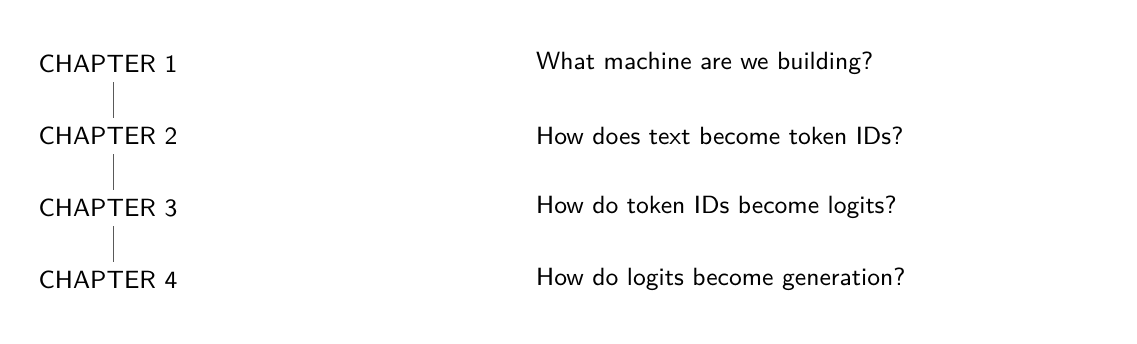
\begin{tikzpicture}[x=6.2pt,y=-13pt,draw=black!65,line width=.45pt]
\path[use as bounding box] (-1,-1) rectangle (62,7);
\node[anchor=west,inner sep=0pt,font=\sffamily\fontsize{9}{11}\selectfont] at (-0.4,0) {\begin{adjustbox}{max width=55.800000000000004pt}CHAPTER 1\end{adjustbox}};
\node[anchor=west,inner sep=0pt,font=\sffamily\fontsize{9}{11}\selectfont] at (28.6,0) {\begin{adjustbox}{max width=179.8pt}What machine are we building?\end{adjustbox}};
\draw (4,1) -- (4,0.5);
\draw (4,1) -- (4,1.5);
\node[anchor=west,inner sep=0pt,font=\sffamily\fontsize{9}{11}\selectfont] at (-0.4,2) {\begin{adjustbox}{max width=55.800000000000004pt}CHAPTER 2\end{adjustbox}};
\node[anchor=west,inner sep=0pt,font=\sffamily\fontsize{9}{11}\selectfont] at (28.6,2) {\begin{adjustbox}{max width=192.20000000000002pt}How does text become token IDs?\end{adjustbox}};
\draw (4,3) -- (4,2.5);
\draw (4,3) -- (4,3.5);
\node[anchor=west,inner sep=0pt,font=\sffamily\fontsize{9}{11}\selectfont] at (-0.4,4) {\begin{adjustbox}{max width=55.800000000000004pt}CHAPTER 3\end{adjustbox}};
\node[anchor=west,inner sep=0pt,font=\sffamily\fontsize{9}{11}\selectfont] at (28.6,4) {\begin{adjustbox}{max width=192.20000000000002pt}How do token IDs become logits?\end{adjustbox}};
\draw (4,5) -- (4,4.5);
\draw (4,5) -- (4,5.5);
\node[anchor=west,inner sep=0pt,font=\sffamily\fontsize{9}{11}\selectfont] at (-0.4,6) {\begin{adjustbox}{max width=55.800000000000004pt}CHAPTER 4\end{adjustbox}};
\node[anchor=west,inner sep=0pt,font=\sffamily\fontsize{9}{11}\selectfont] at (28.6,6) {\begin{adjustbox}{max width=198.4pt}How do logits become generation?\end{adjustbox}};
\end{tikzpicture}
\end{adjustbox}\end{center}

The Part I engine is now:

\begin{center}\begin{adjustbox}{max width=\linewidth}% Legacy topology preserved as native vectors and typeset labels.
\begin{tikzpicture}[x=6.2pt,y=-13pt,draw=black!65,line width=.45pt]
\path[use as bounding box] (-1,-1) rectangle (37,33);
\node[anchor=west,inner sep=0pt,font=\sffamily\fontsize{9}{11}\selectfont] at (-0.4,0) {\begin{adjustbox}{max width=62.0pt}Human text\end{adjustbox}};
\draw (4,1) -- (4,0.5);
\draw (4,1) -- (4,1.5);
\draw[-{Latex[length=2pt,width=3pt]}] (4,1.5) -- (4,2.5);
\node[anchor=west,inner sep=0pt,font=\sffamily\fontsize{9}{11}\selectfont] at (-0.4,3) {\begin{adjustbox}{max width=55.800000000000004pt}Tokenizer\end{adjustbox}};
\draw (4,4) -- (4,3.5);
\draw (4,4) -- (4,4.5);
\draw[-{Latex[length=2pt,width=3pt]}] (4,4.5) -- (4,5.5);
\node[anchor=west,inner sep=0pt,font=\sffamily\fontsize{9}{11}\selectfont] at (-0.4,6) {\begin{adjustbox}{max width=55.800000000000004pt}Token IDs\end{adjustbox}};
\draw (4,7) -- (4,6.5);
\draw (4,7) -- (4,7.5);
\draw[-{Latex[length=2pt,width=3pt]}] (4,7.5) -- (4,8.5);
\node[anchor=west,inner sep=0pt,font=\sffamily\fontsize{9}{11}\selectfont] at (-0.4,9) {\begin{adjustbox}{max width=179.8pt}Tiny numerical language model\end{adjustbox}};
\draw (4,10) -- (4,9.5);
\draw (4,10) -- (4,10.5);
\draw[-{Latex[length=2pt,width=3pt]}] (4,10.5) -- (4,11.5);
\node[anchor=west,inner sep=0pt,font=\sffamily\fontsize{9}{11}\selectfont] at (-0.4,12) {\begin{adjustbox}{max width=223.20000000000002pt}Embedding lookup + output projection\end{adjustbox}};
\draw (4,13) -- (4,12.5);
\draw (4,13) -- (4,13.5);
\draw[-{Latex[length=2pt,width=3pt]}] (4,13.5) -- (4,14.5);
\node[anchor=west,inner sep=0pt,font=\sffamily\fontsize{9}{11}\selectfont] at (-0.4,15) {\begin{adjustbox}{max width=62.0pt}Raw logits\end{adjustbox}};
\draw (4,16) -- (4,15.5);
\draw (4,16) -- (4,16.5);
\draw[-{Latex[length=2pt,width=3pt]}] (4,16.5) -- (4,17.5);
\node[anchor=west,inner sep=0pt,font=\sffamily\fontsize{9}{11}\selectfont] at (-0.4,18) {\begin{adjustbox}{max width=93.0pt}Sampling policy\end{adjustbox}};
\draw (4,19) -- (4,18.5);
\draw (4,19) -- (4,19.5);
\draw[-{Latex[length=2pt,width=3pt]}] (4,19.5) -- (4,20.5);
\draw (13,21) -- (12.5,21);
\draw (13,21) -- (13.5,21);
\draw (14,21) -- (13.5,21);
\draw (14,21) -- (14.5,21);
\draw (15,21) -- (14.5,21);
\draw (15,21) -- (15.5,21);
\draw (16,21) -- (15.5,21);
\draw (16,21) -- (16.5,21);
\draw (17,21) -- (16.5,21);
\draw (17,21) -- (17.5,21);
\draw (18,21) -- (17.5,21);
\draw (18,21) -- (18.5,21);
\draw (19,21) -- (18.5,21);
\draw (19,21) -- (19.5,21);
\draw (20,21) -- (19.5,21);
\draw (20,21) -- (20.5,21);
\draw (21,21) -- (20.5,21);
\draw (21,21) -- (21.5,21);
\draw (22,21) -- (21.5,21);
\draw (22,21) -- (22,21.5);
\node[anchor=west,inner sep=0pt,font=\sffamily\fontsize{9}{11}\selectfont] at (-0.4,21) {\begin{adjustbox}{max width=74.4pt}Next TokenId\end{adjustbox}};
\draw (4,22) -- (4,21.5);
\draw (4,22) -- (4,22.5);
\draw (22,22) -- (22,21.5);
\draw (22,22) -- (22,22.5);
\draw[-{Latex[length=2pt,width=3pt]}] (4,22.5) -- (4,23.5);
\draw (22,23) -- (22,22.5);
\draw (22,23) -- (22,23.5);
\draw (22,24) -- (22,23.5);
\draw (22,24) -- (22,24.5);
\node[anchor=west,inner sep=0pt,font=\sffamily\fontsize{9}{11}\selectfont] at (-0.4,24) {\begin{adjustbox}{max width=74.4pt}Decode bytes\end{adjustbox}};
\draw (4,25) -- (4,24.5);
\draw (4,25) -- (4,25.5);
\draw (22,25) -- (22,24.5);
\draw (22,25) -- (22,25.5);
\draw[-{Latex[length=2pt,width=3pt]}] (4,25.5) -- (4,26.5);
\draw (22,26) -- (22,25.5);
\draw (22,26) -- (22,26.5);
\draw (22,27) -- (22,26.5);
\draw (22,27) -- (22,27.5);
\node[anchor=west,inner sep=0pt,font=\sffamily\fontsize{9}{11}\selectfont] at (-0.4,27) {\begin{adjustbox}{max width=74.4pt}UTF-8 stream\end{adjustbox}};
\draw (4,28) -- (4,27.5);
\draw (4,28) -- (4,28.5);
\draw (22,28) -- (22,27.5);
\draw (22,28) -- (22,28.5);
\draw[-{Latex[length=2pt,width=3pt]}] (4,28.5) -- (4,29.5);
\draw (22,29) -- (22,28.5);
\draw (22,29) -- (22,29.5);
\draw (22,30) -- (22,29.5);
\draw (22,30) -- (22,30.5);
\node[anchor=west,inner sep=0pt,font=\sffamily\fontsize{9}{11}\selectfont] at (-0.4,30) {\begin{adjustbox}{max width=74.4pt}Human output\end{adjustbox}};
\draw (22,31) -- (22,30.5);
\draw (22,31) -- (22,31.5);
\draw[-{Latex[length=2pt,width=3pt]}] (18.5,32) -- (17.5,32);
\draw (19,32) -- (18.5,32);
\draw (19,32) -- (19.5,32);
\draw (20,32) -- (19.5,32);
\draw (20,32) -- (20.5,32);
\draw (21,32) -- (20.5,32);
\draw (21,32) -- (21.5,32);
\draw (22,32) -- (21.5,32);
\draw (22,32) -- (22,31.5);
\node[anchor=west,inner sep=0pt,font=\sffamily\fontsize{9}{11}\selectfont] at (-0.4,32) {\begin{adjustbox}{max width=105.4pt}append to history\end{adjustbox}};
\end{tikzpicture}
\end{adjustbox}\end{center}

It is tiny. It is scalar. It has only four tokens. It depends only on
the final token. It does no training, attention, position handling, KV
caching, GGUF loading, quantization, batching, paging, native kernels,
or acceleration.

Those limitations do not make it fake. Every parameter is visible. Every
forward score is real. Every selection follows a stated policy. Every
random draw has an owner. Every output token feeds back. Every request
terminates once. A reader can inspect and run the entire path.

\begin{quote}
\textbf{FIRST PRINCIPLE} Autoregressive generation feeds selected
outputs back into future model inputs, and every such loop needs
explicit state and termination ownership.
\end{quote}

\subsection{Summary}\label{summary-3}

\begin{itemize}
\tightlist
\item
  A model produces raw logits; a sampler chooses a token.
\item
  Softmax converts finite scores to non-negative probability mass
  summing approximately to one.
\item
  Subtracting the maximum preserves softmax and prevents exponential
  overflow.
\item
  Greedy selection uses one argmax scan and needs no softmax.
\item
  Categorical selection maps a draw in \texttt{{[}0,1)} through
  cumulative intervals.
\item
  Temperature changes distribution sharpness; it does not add randomness
  or change ordering when positive.
\item
  Top-k keeps a fixed number of high scores; top-p keeps adaptive
  probability mass and includes the threshold-crossing candidate.
\item
  Operation order is part of inference behavior.
\item
  Raw logits and processed candidates are separate artifacts.
\item
  RNG state belongs to one request. A seed has a bounded reproduction
  contract, not a universal guarantee.
\item
  ENGINE-1 checks EOS before commit, counts only new visible tokens
  against the output budget, and checks cancellation at defined
  boundaries.
\item
  One lifecycle owner emits exactly one completed, cancelled, or failed
  terminal outcome.
\item
  Part I now contains the smallest complete inference engine.
\end{itemize}

\subsection{Part II preview: tensors without
magic}\label{part-ii-preview-tensors-without-magic}

ENGINE-1's remaining intellectual defect is now impossible to miss. It
feeds tokens back, but its model still reads only the final token. A
modern decoder needs internal representations spanning positions and
hidden dimensions.

Before attention, queries, keys, values, or Transformer layers, we need
to know how those numbers occupy memory. Chapter 5 begins Part II with
scalars, vectors, matrices, tensors, rank, shape, dtype, row-major
layout, stride, contiguity, offset calculation, views, copies, aliases,
ownership, bounds, and overflow-safe element counts.

Attention comes later. First we build a tensor substrate whose semantics
can survive it.

\subsection{References}\label{references-1}

\begin{itemize}
\tightlist
\item
  Yoshua Bengio, Réjean Ducharme, Pascal Vincent, and Christian Jauvin.
  \href{https://jmlr.org/papers/v3/bengio03a.html}{A Neural
  Probabilistic Language Model}. \emph{Journal of Machine Learning
  Research} 3, 2003.
\item
  Ari Holtzman, Jan Buys, Li Du, Maxwell Forbes, and Yejin Choi.
  \href{https://arxiv.org/abs/1904.09751}{The Curious Case of Neural
  Text Degeneration}. ICLR

  \begin{enumerate}
  \def\labelenumi{\arabic{enumi}.}
  \setcounter{enumi}{2019}
  \tightlist
  \item
  \end{enumerate}
\item
  Pierre Blanchard, Desmond J. Higham, and Nicholas J. Higham.
  \href{https://doi.org/10.1093/imanum/draa038}{Accurately computing the
  log-sum-exp and softmax functions}. \emph{IMA Journal of Numerical
  Analysis} 41(4), 2021.
\item
  Guy L. Steele Jr., Doug Lea, and Christine H. Flood.
  \href{https://doi.org/10.1145/2660193.2660195}{Fast Splittable
  Pseudorandom Number Generators}. OOPSLA 2014.
\item
  PyTorch.
  \href{https://docs.pytorch.org/docs/stable/generated/torch.nn.Softmax.html}{\texttt{\seqsplit{torch.nn.Softmax}}
  documentation}.
\item
  Hermon source at
  \texttt{\seqsplit{472a44cdb511b2dae6c9569e59543db8f8350b25}}.
\item
  llama.cpp source at
  \texttt{\seqsplit{389ff61d77b5c71cec0cf92fe4e5d01ace80b797}}.
\end{itemize}

\clearpage

\section{Chapter 5 --- Tensors Without
Magic}\label{chapter-5-tensors-without-magic}

Part I ended with a complete loop. Text became token IDs. A tiny
language model turned the last ID into an embedding, multiplied that
activation by an output projection, produced logits, and fed a selected
token back into the next step. Every number was small enough to print.
Every array was short enough to count.

That convenience hid a systems problem. The model stored its embedding
in a \texttt{Vec\textless{}f32\textgreater{}}, yet the vector itself did
not say that its logical shape was \texttt{{[}vocabulary,\ hidden{]}}.
The projection used another \texttt{Vec\textless{}f32\textgreater{}}. A
comment and a pair of loop bounds carried the missing meaning. If those
facts ever disagreed, the bytes could remain finite and the program
could still compute the wrong answer.

This chapter gives those bytes a contract. It does not build a tensor
framework or perform matrix multiplication. It builds the smallest
substrate on which the rest of Part II can reason honestly about memory.

\begin{quote}
\textbf{FIRST PRINCIPLE} Mathematics tells us \emph{what} value we need.
Tensor layout tells the machine \emph{where} that value lives.
\end{quote}

\subsection{Where we are: from a model equation to six stored
values}\label{where-we-are-from-a-model-equation-to-six-stored-values}

Follow the engine downward: a request invokes a model; the model asks an
operator to read tensors; the operator must find the right bytes. This
chapter works at that final representation boundary. Chapter 6 will put
arithmetic on top of it. The current repository already contains later
chapters, but this chapter's executable contract remains Tensor
Substrate v1.

\begin{figure}[H]\centering\resizebox{\linewidth}{!}{% Generated from figures/generated/tensor.svg; do not hand edit.
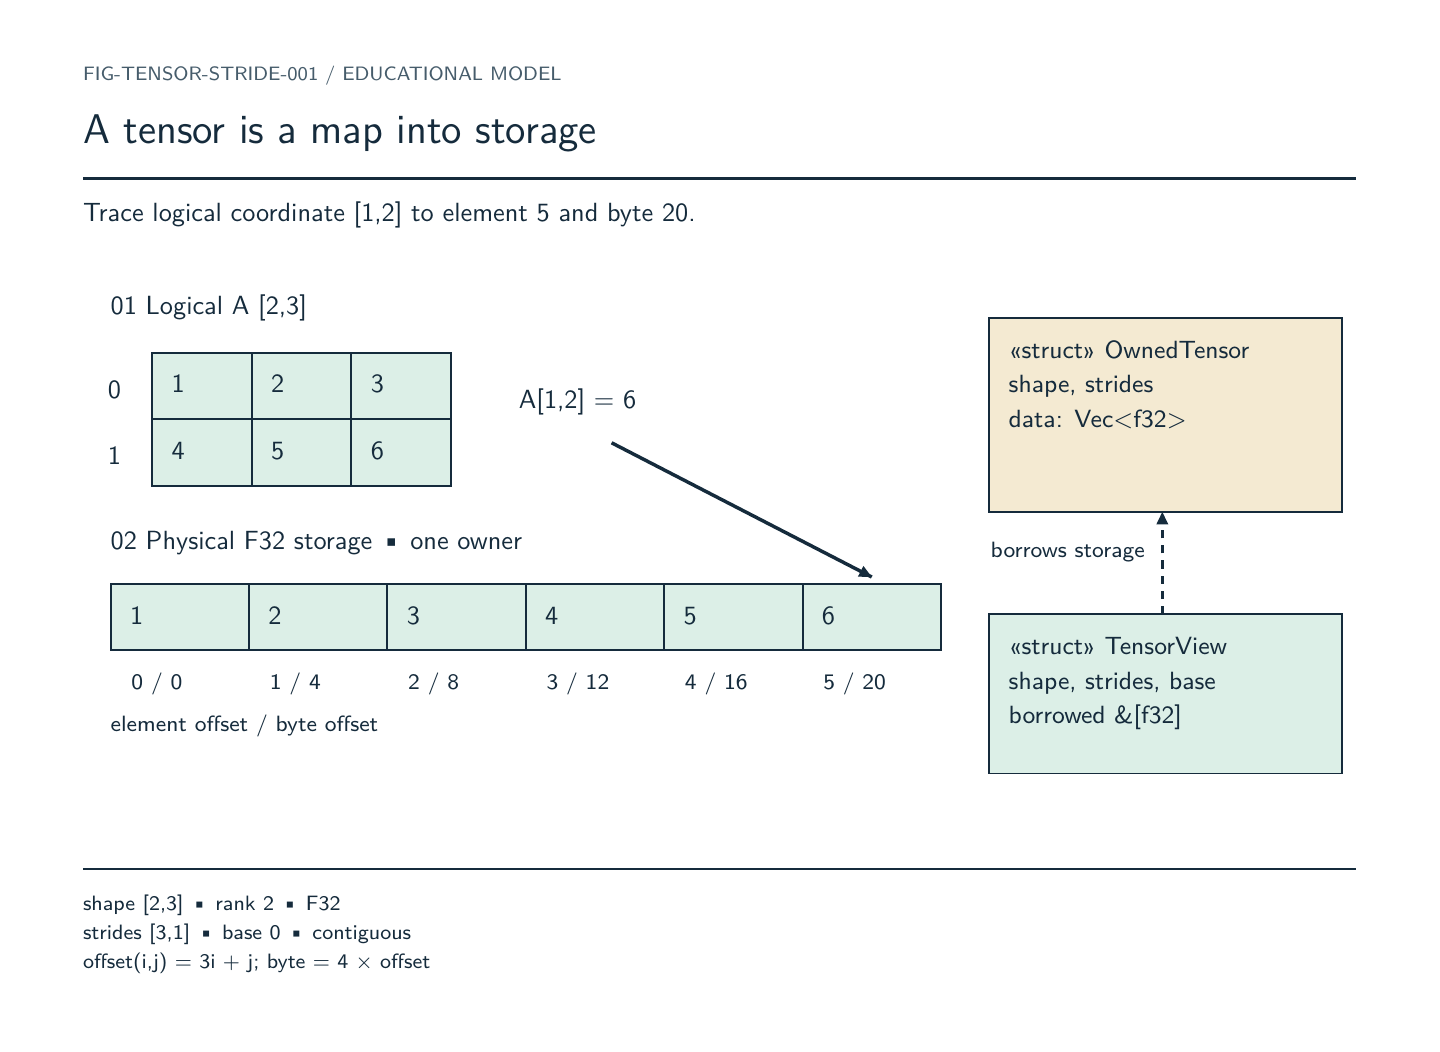
\begin{tikzpicture}[x=.5pt,y=-.5pt]
\path[use as bounding box] (0,0) rectangle (1000,720);
\path[fill=white,draw=none,line width=0.5pt] (0.0,0.0) rectangle (1000.0,720.0);
\node[inner sep=0pt,outer sep=0pt,anchor=base west,text={rgb,255:red,70;green,92;blue,107},font=\sffamily\fontsize{7.0}{8.4}\selectfont] at (40,38) {FIG-TENSOR-STRIDE-001  /  EDUCATIONAL MODEL};
\node[inner sep=0pt,outer sep=0pt,anchor=base west,text={rgb,255:red,21;green,43;blue,60},font=\sffamily\fontsize{15.0}{18.0}\selectfont] at (40,84) {A tensor is a map into storage};
\draw[fill=none,draw={rgb,255:red,21;green,43;blue,60},line width=0.75pt] (40,109) -- (960,109);
\node[inner sep=0pt,outer sep=0pt,anchor=base west,text={rgb,255:red,21;green,43;blue,60},font=\sffamily\fontsize{9.5}{11.4}\selectfont] at (40,140) {Trace logical coordinate [1,2] to element 5 and byte 20.};
\node[inner sep=0pt,outer sep=0pt,anchor=base west,text={rgb,255:red,21;green,43;blue,60},font=\sffamily\fontsize{9.5}{11.4}\selectfont] at (60,207) {01  Logical A [2,3]};
\path[fill={rgb,255:red,220;green,239;blue,231},draw={rgb,255:red,21;green,43;blue,60},line width=0.7pt] (90.0,235.0) rectangle (162.0,283.0);
\node[inner sep=0pt,outer sep=0pt,anchor=base west,text={rgb,255:red,21;green,43;blue,60},font=\sffamily\fontsize{9.5}{11.4}\selectfont] at (104,264) {1};
\path[fill={rgb,255:red,220;green,239;blue,231},draw={rgb,255:red,21;green,43;blue,60},line width=0.7pt] (162.0,235.0) rectangle (234.0,283.0);
\node[inner sep=0pt,outer sep=0pt,anchor=base west,text={rgb,255:red,21;green,43;blue,60},font=\sffamily\fontsize{9.5}{11.4}\selectfont] at (176,264) {2};
\path[fill={rgb,255:red,220;green,239;blue,231},draw={rgb,255:red,21;green,43;blue,60},line width=0.7pt] (234.0,235.0) rectangle (306.0,283.0);
\node[inner sep=0pt,outer sep=0pt,anchor=base west,text={rgb,255:red,21;green,43;blue,60},font=\sffamily\fontsize{9.5}{11.4}\selectfont] at (248,264) {3};
\path[fill={rgb,255:red,220;green,239;blue,231},draw={rgb,255:red,21;green,43;blue,60},line width=0.7pt] (90.0,283.0) rectangle (162.0,331.0);
\node[inner sep=0pt,outer sep=0pt,anchor=base west,text={rgb,255:red,21;green,43;blue,60},font=\sffamily\fontsize{9.5}{11.4}\selectfont] at (104,312) {4};
\path[fill={rgb,255:red,220;green,239;blue,231},draw={rgb,255:red,21;green,43;blue,60},line width=0.7pt] (162.0,283.0) rectangle (234.0,331.0);
\node[inner sep=0pt,outer sep=0pt,anchor=base west,text={rgb,255:red,21;green,43;blue,60},font=\sffamily\fontsize{9.5}{11.4}\selectfont] at (176,312) {5};
\path[fill={rgb,255:red,220;green,239;blue,231},draw={rgb,255:red,21;green,43;blue,60},line width=0.7pt] (234.0,283.0) rectangle (306.0,331.0);
\node[inner sep=0pt,outer sep=0pt,anchor=base west,text={rgb,255:red,21;green,43;blue,60},font=\sffamily\fontsize{9.5}{11.4}\selectfont] at (248,312) {6};
\node[inner sep=0pt,outer sep=0pt,anchor=base west,text={rgb,255:red,21;green,43;blue,60},font=\sffamily\fontsize{9.5}{11.4}\selectfont] at (58,268) {0};
\node[inner sep=0pt,outer sep=0pt,anchor=base west,text={rgb,255:red,21;green,43;blue,60},font=\sffamily\fontsize{9.5}{11.4}\selectfont] at (58,316) {1};
\node[inner sep=0pt,outer sep=0pt,anchor=base west,text={rgb,255:red,21;green,43;blue,60},font=\sffamily\fontsize{9.5}{11.4}\selectfont] at (355,275) {A[1,2] = 6};
\draw[fill=none,draw={rgb,255:red,21;green,43;blue,60},line width=1.25pt] (422,300) -- (610,397);
\path[fill={rgb,255:red,21;green,43;blue,60},draw=none,line width=0.5pt] (610.00,397.00) -- (600.00,396.74) -- (603.99,389.01) -- cycle;
\node[inner sep=0pt,outer sep=0pt,anchor=base west,text={rgb,255:red,21;green,43;blue,60},font=\sffamily\fontsize{9.5}{11.4}\selectfont] at (60,377) {02  Physical F32 storage • one owner};
\path[fill={rgb,255:red,220;green,239;blue,231},draw={rgb,255:red,21;green,43;blue,60},line width=0.7pt] (60.0,402.0) rectangle (160.0,450.0);
\node[inner sep=0pt,outer sep=0pt,anchor=base west,text={rgb,255:red,21;green,43;blue,60},font=\sffamily\fontsize{9.5}{11.4}\selectfont] at (74,431) {1};
\path[fill={rgb,255:red,220;green,239;blue,231},draw={rgb,255:red,21;green,43;blue,60},line width=0.7pt] (160.0,402.0) rectangle (260.0,450.0);
\node[inner sep=0pt,outer sep=0pt,anchor=base west,text={rgb,255:red,21;green,43;blue,60},font=\sffamily\fontsize{9.5}{11.4}\selectfont] at (174,431) {2};
\path[fill={rgb,255:red,220;green,239;blue,231},draw={rgb,255:red,21;green,43;blue,60},line width=0.7pt] (260.0,402.0) rectangle (360.0,450.0);
\node[inner sep=0pt,outer sep=0pt,anchor=base west,text={rgb,255:red,21;green,43;blue,60},font=\sffamily\fontsize{9.5}{11.4}\selectfont] at (274,431) {3};
\path[fill={rgb,255:red,220;green,239;blue,231},draw={rgb,255:red,21;green,43;blue,60},line width=0.7pt] (360.0,402.0) rectangle (460.0,450.0);
\node[inner sep=0pt,outer sep=0pt,anchor=base west,text={rgb,255:red,21;green,43;blue,60},font=\sffamily\fontsize{9.5}{11.4}\selectfont] at (374,431) {4};
\path[fill={rgb,255:red,220;green,239;blue,231},draw={rgb,255:red,21;green,43;blue,60},line width=0.7pt] (460.0,402.0) rectangle (560.0,450.0);
\node[inner sep=0pt,outer sep=0pt,anchor=base west,text={rgb,255:red,21;green,43;blue,60},font=\sffamily\fontsize{9.5}{11.4}\selectfont] at (474,431) {5};
\path[fill={rgb,255:red,220;green,239;blue,231},draw={rgb,255:red,21;green,43;blue,60},line width=0.7pt] (560.0,402.0) rectangle (660.0,450.0);
\node[inner sep=0pt,outer sep=0pt,anchor=base west,text={rgb,255:red,21;green,43;blue,60},font=\sffamily\fontsize{9.5}{11.4}\selectfont] at (574,431) {6};
\node[inner sep=0pt,outer sep=0pt,anchor=base west,text={rgb,255:red,21;green,43;blue,60},font=\sffamily\fontsize{8.0}{9.6}\selectfont] at (75,478) {0 / 0};
\node[inner sep=0pt,outer sep=0pt,anchor=base west,text={rgb,255:red,21;green,43;blue,60},font=\sffamily\fontsize{8.0}{9.6}\selectfont] at (175,478) {1 / 4};
\node[inner sep=0pt,outer sep=0pt,anchor=base west,text={rgb,255:red,21;green,43;blue,60},font=\sffamily\fontsize{8.0}{9.6}\selectfont] at (275,478) {2 / 8};
\node[inner sep=0pt,outer sep=0pt,anchor=base west,text={rgb,255:red,21;green,43;blue,60},font=\sffamily\fontsize{8.0}{9.6}\selectfont] at (375,478) {3 / 12};
\node[inner sep=0pt,outer sep=0pt,anchor=base west,text={rgb,255:red,21;green,43;blue,60},font=\sffamily\fontsize{8.0}{9.6}\selectfont] at (475,478) {4 / 16};
\node[inner sep=0pt,outer sep=0pt,anchor=base west,text={rgb,255:red,21;green,43;blue,60},font=\sffamily\fontsize{8.0}{9.6}\selectfont] at (575,478) {5 / 20};
\node[inner sep=0pt,outer sep=0pt,anchor=base west,text={rgb,255:red,21;green,43;blue,60},font=\sffamily\fontsize{8.0}{9.6}\selectfont] at (60,509) {element offset / byte offset};
\path[fill={rgb,255:red,244;green,234;blue,210},draw={rgb,255:red,21;green,43;blue,60},line width=0.7pt] (695.0,210.0) rectangle (950.0,350.0);
\node[inner sep=0pt,outer sep=0pt,anchor=base west,text={rgb,255:red,21;green,43;blue,60},font=\sffamily\fontsize{9.0}{10.799999999999999}\selectfont] at (709,239) {«struct» OwnedTensor};
\node[inner sep=0pt,outer sep=0pt,anchor=base west,text={rgb,255:red,21;green,43;blue,60},font=\sffamily\fontsize{9.0}{10.799999999999999}\selectfont] at (709,264) {shape, strides};
\node[inner sep=0pt,outer sep=0pt,anchor=base west,text={rgb,255:red,21;green,43;blue,60},font=\sffamily\fontsize{9.0}{10.799999999999999}\selectfont] at (709,289) {data: Vec<f32>};
\path[fill={rgb,255:red,220;green,239;blue,231},draw={rgb,255:red,21;green,43;blue,60},line width=0.7pt] (695.0,424.0) rectangle (950.0,539.0);
\node[inner sep=0pt,outer sep=0pt,anchor=base west,text={rgb,255:red,21;green,43;blue,60},font=\sffamily\fontsize{9.0}{10.799999999999999}\selectfont] at (709,453) {«struct» TensorView};
\node[inner sep=0pt,outer sep=0pt,anchor=base west,text={rgb,255:red,21;green,43;blue,60},font=\sffamily\fontsize{9.0}{10.799999999999999}\selectfont] at (709,478) {shape, strides, base};
\node[inner sep=0pt,outer sep=0pt,anchor=base west,text={rgb,255:red,21;green,43;blue,60},font=\sffamily\fontsize{9.0}{10.799999999999999}\selectfont] at (709,503) {borrowed \&[f32]};
\draw[fill=none,draw={rgb,255:red,21;green,43;blue,60},line width=1.25pt,dash pattern=on 3.0pt off 2.5pt] (820,424) -- (820,350);
\path[fill={rgb,255:red,21;green,43;blue,60},draw=none,line width=0.5pt] (820.00,350.00) -- (824.35,359.00) -- (815.65,359.00) -- cycle;
\node[inner sep=0pt,outer sep=0pt,anchor=base west,text={rgb,255:red,21;green,43;blue,60},font=\sffamily\fontsize{8.0}{9.6}\selectfont] at (696,383) {borrows storage};
\draw[fill=none,draw={rgb,255:red,21;green,43;blue,60},line width=0.75pt] (40,608) -- (960,608);
\node[inner sep=0pt,outer sep=0pt,anchor=base west,text={rgb,255:red,21;green,43;blue,60},font=\sffamily\fontsize{7.5}{9.0}\selectfont] at (40,638) {shape [2,3] • rank 2 • F32};
\node[inner sep=0pt,outer sep=0pt,anchor=base west,text={rgb,255:red,21;green,43;blue,60},font=\sffamily\fontsize{7.5}{9.0}\selectfont] at (40,659) {strides [3,1] • base 0 • contiguous};
\node[inner sep=0pt,outer sep=0pt,anchor=base west,text={rgb,255:red,21;green,43;blue,60},font=\sffamily\fontsize{7.5}{9.0}\selectfont] at (40,680) {offset(i,j) = 3i + j; byte = 4 × offset};
\end{tikzpicture}
}\caption{Logical coordinates reach physical storage through explicit strides and a base offset.}\end{figure}

Our recurring matrix is \(\mathbf{A}\in\mathbb{R}^{2\times3}\), with
first row \texttt{{[}1,2,3{]}} and second row \texttt{{[}4,5,6{]}}. Its
owner holds six F32 elements, or 24 payload bytes. The first plate
connects the logical coordinate \texttt{{[}1,2{]}} to element offset 5
and byte displacement 20. Neither number is an allocator address. The
actual allocation may live anywhere suitable for \texttt{f32}.

Watch three things separately as the chapter proceeds: which logical
value a coordinate selects, which storage slot supplies it, and which
object owns that slot. Transpose changes the first relationship without
moving the payload. Materialization creates a second owner. Reshape can
have the same output shape as transpose while selecting different
values. Those differences are the mechanism, not details to hide under a
framework method name.

The plates have
\href{https://github.com/hermonai/inside-the-llm-engine/blob/astra-visual-rewrite/figures/chapter05-atlas.md}{plain-text
equivalents} and a
\href{https://github.com/hermonai/inside-the-llm-engine/blob/astra-visual-rewrite/code/reference/fixtures/chapter05-visual.json}{shared
executable fixture}. The original letter-valued and higher-rank
exercises remain useful independent checks. The main visual journey now
uses the same six numbers throughout.

\subsection{The vector that could not tell the
truth}\label{the-vector-that-could-not-tell-the-truth}

Suppose a loader hands us twelve \texttt{f32} values. What tensor did it
load?

\begin{verbatim}
[12]       [3, 4]       [4, 3]       [2, 2, 3]       [1, 3, 4]
\end{verbatim}

Every listed shape has twelve elements. They do not have the same axes
or indexing semantics. Even shape \texttt{{[}3,4{]}} does not tell us
whether adjacent bytes move across a row, down a column, or through some
strided view of a larger allocation. Twelve scalar payloads are evidence
about storage length, not a complete tensor description.

For every tensor in this book, ask five questions:

\begin{enumerate}
\def\labelenumi{\arabic{enumi}.}
\tightlist
\item
  What is its shape?
\item
  What is its dtype?
\item
  What is its physical layout?
\item
  Who owns the underlying bytes?
\item
  How long may a view reference those bytes?
\end{enumerate}

Later we will add location---CPU memory, device memory, mapped file, or
another tier. Chapter 5 stays in local CPU memory so we can settle the
first five without hiding them behind a device abstraction.

\subsection{From scalar to tensor}\label{from-scalar-to-tensor}

A \textbf{scalar} is one value and has rank 0. A \textbf{vector} has one
logical axis and rank 1. A \textbf{matrix} has two axes and rank 2. We
use \textbf{tensor} for the general case: a typed multidimensional array
with explicit shape and layout semantics.

{\def\LTcaptype{none} % do not increment counter
\begin{longtable}[]{@{}
  >{\raggedright\arraybackslash}p{(\linewidth - 6\tabcolsep) * \real{0.2308}}
  >{\raggedright\arraybackslash}p{(\linewidth - 6\tabcolsep) * \real{0.2308}}
  >{\raggedright\arraybackslash}p{(\linewidth - 6\tabcolsep) * \real{0.2308}}
  >{\raggedleft\arraybackslash}p{(\linewidth - 6\tabcolsep) * \real{0.3077}}@{}}
\toprule\noalign{}
\begin{minipage}[b]{\linewidth}\raggedright
Object
\end{minipage} & \begin{minipage}[b]{\linewidth}\raggedright
Example
\end{minipage} & \begin{minipage}[b]{\linewidth}\raggedright
Shape
\end{minipage} & \begin{minipage}[b]{\linewidth}\raggedleft
Tensor rank
\end{minipage} \\
\midrule\noalign{}
\endhead
\bottomrule\noalign{}
\endlastfoot
Scalar & \texttt{42.0} & \texttt{{[}{]}} & 0 \\
Vector & \texttt{{[}1,2,3{]}} & \texttt{{[}3{]}} & 1 \\
Matrix & three rows, two columns & \texttt{{[}3,2{]}} & 2 \\
Higher-rank tensor & two batches of three-by-four values &
\texttt{{[}2,3,4{]}} & 3 \\
\end{longtable}
}

Here \textbf{rank} means number of logical axes. Linear algebra also
uses \emph{matrix rank} for the dimension of a matrix's row or column
space. These are different concepts. A shape \texttt{{[}3,2{]}} tensor
always has tensor rank 2, even if all its rows are linearly dependent.

If a rank-\(r\) tensor has shape

\[
\mathbf{d} = [d_0,d_1,\ldots,d_{r-1}],
\]

then \(d_a\) is the length of axis \(a\). A later activation might use
named axes such as \texttt{{[}batch,\ token,\ hidden{]}}; the names
explain model meaning while the integer dimensions define valid indices.

\subsection{Element count is checked
arithmetic}\label{element-count-is-checked-arithmetic}

The number of logical elements is the product of all dimensions:

\[
N(\mathbf{d}) = \prod_{a=0}^{r-1} d_a.
\]

For shape \texttt{{[}3,4{]}}, \(N=12\). For rank 0, the empty product is
one, so shape \texttt{{[}{]}} describes one scalar. This definition is
mathematically compact, but a systems implementation must ask whether
the product fits its integer type.

\begin{verbatim}
shape.iter().try_fold(1_usize, |count, &dimension| {
    count.checked_mul(dimension).ok_or(TensorError::ShapeOverflow)
})
\end{verbatim}

The real implementation handles zero dimensions first, then uses checked
multiplication. It also checks the byte count:

\[
B=N(\mathbf{d})\,w_{\mathrm{dtype}}\quad[\mathrm{bytes}],
\]

where \(w_{\mathrm{dtype}}\) is bytes per stored element.

Here \(B\) is bytes, not elements. For \texttt{{[}2,3,4{]}} in
\texttt{f32}, \(N=24\) elements and \(B=24\times4=96\) bytes. Both
products can overflow independently.

\begin{quote}
\textbf{ENGINEERING FAILURE --- WRAPPED SIZE} External metadata claims
shape \texttt{{[}usize::MAX,2{]}}. Unchecked multiplication wraps to a
small value, code allocates too little storage, and later address
arithmetic trusts the original dimensions. Checked size arithmetic is
not defensive decoration; it is part of model-loading security.
\end{quote}

\subsection{Zero-sized dimensions are
deliberate}\label{zero-sized-dimensions-are-deliberate}

Tensor Substrate v1 permits zero-sized dimensions. Shape
\texttt{{[}0,4{]}} has zero elements and owns an empty vector. It has
rank 2, canonical strides \texttt{{[}4,1{]}}, and no valid logical index
because index 0 is already outside axis 0.

This decision keeps shape algebra honest. Empty batches and empty slices
can be represented without a sentinel. A zero-element view may have its
base offset at the end of storage, because it reaches no element. It may
reshape only to a shape whose checked element count is also zero.

Allowing empty tensors does not disable all validation. Canonical stride
products still have to fit \texttt{usize}; malformed metadata cannot
smuggle an unrepresentable layout through a zero dimension.

\subsection{Dtype is interpretation, not
width}\label{dtype-is-interpretation-not-width}

A \textbf{dtype} specifies how stored bits represent values and
participate in arithmetic. Tensor Substrate v1 implements only
\texttt{F32}. Each element is one IEEE-754 binary32 value and occupies
four bytes, while reductions in later operators may choose a different
accumulation type.

Other systems use \texttt{f16}, \texttt{bf16}, integers, and packed
quantized formats. Two types can occupy the same byte width yet
interpret bits differently. A packed quantized block may represent many
logical weights with shared scale metadata, so ``one scalar equals one
fixed byte range'' eventually stops being a useful model. Chapter 16
will face that complexity. Adding a generic dtype hierarchy now would
create machinery without a chapter requirement.

\texttt{DType::F32} is still explicit in v1. That apparently redundant
name prevents future code from treating
\texttt{\seqsplit{size\_of::<f32>()}} as the whole semantic contract.

\subsection{Logical values and physical
storage}\label{logical-values-and-physical-storage}

Consider this logical matrix:

\[
\mathbf{A} =
\begin{bmatrix}
1 & 2 & 3 \\
4 & 5 & 6
\end{bmatrix},
\qquad \mathbf{A}\in\mathbb{R}^{2\times3}.
\]

A canonical row-major representation places each row consecutively:

\begin{center}\begin{adjustbox}{max width=\linewidth}% Legacy topology preserved as native vectors and typeset labels.
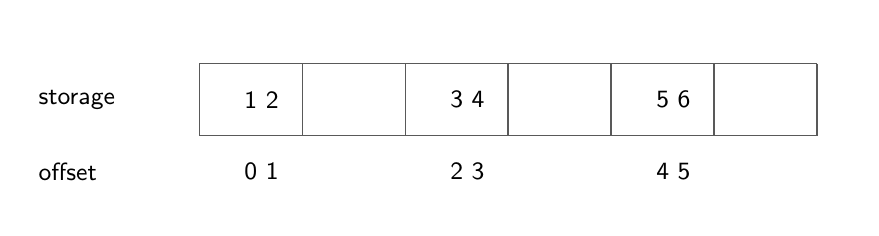
\begin{tikzpicture}[x=6.2pt,y=-13pt,draw=black!65,line width=.45pt]
\path[use as bounding box] (-1,-1) rectangle (47,4);
\draw (9,0) -- (9.5,0);
\draw (9,0) -- (9,0.5);
\draw (10,0) -- (9.5,0);
\draw (10,0) -- (10.5,0);
\draw (11,0) -- (10.5,0);
\draw (11,0) -- (11.5,0);
\draw (12,0) -- (11.5,0);
\draw (12,0) -- (12.5,0);
\draw (13,0) -- (12.5,0);
\draw (13,0) -- (13.5,0);
\draw (14,0) -- (13.5,0);
\draw (14,0) -- (14.5,0);
\draw (15,0) -- (14.5,0);
\draw (15,0) -- (15.5,0);
\draw (15,0) -- (15,0.5);
\draw (16,0) -- (15.5,0);
\draw (16,0) -- (16.5,0);
\draw (17,0) -- (16.5,0);
\draw (17,0) -- (17.5,0);
\draw (18,0) -- (17.5,0);
\draw (18,0) -- (18.5,0);
\draw (19,0) -- (18.5,0);
\draw (19,0) -- (19.5,0);
\draw (20,0) -- (19.5,0);
\draw (20,0) -- (20.5,0);
\draw (21,0) -- (20.5,0);
\draw (21,0) -- (21.5,0);
\draw (21,0) -- (21,0.5);
\draw (22,0) -- (21.5,0);
\draw (22,0) -- (22.5,0);
\draw (23,0) -- (22.5,0);
\draw (23,0) -- (23.5,0);
\draw (24,0) -- (23.5,0);
\draw (24,0) -- (24.5,0);
\draw (25,0) -- (24.5,0);
\draw (25,0) -- (25.5,0);
\draw (26,0) -- (25.5,0);
\draw (26,0) -- (26.5,0);
\draw (27,0) -- (26.5,0);
\draw (27,0) -- (27.5,0);
\draw (27,0) -- (27,0.5);
\draw (28,0) -- (27.5,0);
\draw (28,0) -- (28.5,0);
\draw (29,0) -- (28.5,0);
\draw (29,0) -- (29.5,0);
\draw (30,0) -- (29.5,0);
\draw (30,0) -- (30.5,0);
\draw (31,0) -- (30.5,0);
\draw (31,0) -- (31.5,0);
\draw (32,0) -- (31.5,0);
\draw (32,0) -- (32.5,0);
\draw (33,0) -- (32.5,0);
\draw (33,0) -- (33.5,0);
\draw (33,0) -- (33,0.5);
\draw (34,0) -- (33.5,0);
\draw (34,0) -- (34.5,0);
\draw (35,0) -- (34.5,0);
\draw (35,0) -- (35.5,0);
\draw (36,0) -- (35.5,0);
\draw (36,0) -- (36.5,0);
\draw (37,0) -- (36.5,0);
\draw (37,0) -- (37.5,0);
\draw (38,0) -- (37.5,0);
\draw (38,0) -- (38.5,0);
\draw (39,0) -- (38.5,0);
\draw (39,0) -- (39.5,0);
\draw (39,0) -- (39,0.5);
\draw (40,0) -- (39.5,0);
\draw (40,0) -- (40.5,0);
\draw (41,0) -- (40.5,0);
\draw (41,0) -- (41.5,0);
\draw (42,0) -- (41.5,0);
\draw (42,0) -- (42.5,0);
\draw (43,0) -- (42.5,0);
\draw (43,0) -- (43.5,0);
\draw (44,0) -- (43.5,0);
\draw (44,0) -- (44.5,0);
\draw (45,0) -- (44.5,0);
\draw (45,0) -- (45,0.5);
\draw (9,1) -- (9,0.5);
\draw (9,1) -- (9,1.5);
\draw (15,1) -- (15,0.5);
\draw (15,1) -- (15,1.5);
\draw (21,1) -- (21,0.5);
\draw (21,1) -- (21,1.5);
\draw (27,1) -- (27,0.5);
\draw (27,1) -- (27,1.5);
\draw (33,1) -- (33,0.5);
\draw (33,1) -- (33,1.5);
\draw (39,1) -- (39,0.5);
\draw (39,1) -- (39,1.5);
\draw (45,1) -- (45,0.5);
\draw (45,1) -- (45,1.5);
\node[anchor=west,inner sep=0pt,font=\sffamily\fontsize{9}{11}\selectfont] at (-0.4,1) {\begin{adjustbox}{max width=43.4pt}storage\end{adjustbox}};
\node[anchor=west,inner sep=0pt,font=\sffamily\fontsize{9}{11}\selectfont] at (11.6,1) {\begin{adjustbox}{max width=43.4pt}1     2\end{adjustbox}};
\node[anchor=west,inner sep=0pt,font=\sffamily\fontsize{9}{11}\selectfont] at (23.6,1) {\begin{adjustbox}{max width=43.4pt}3     4\end{adjustbox}};
\node[anchor=west,inner sep=0pt,font=\sffamily\fontsize{9}{11}\selectfont] at (35.6,1) {\begin{adjustbox}{max width=43.4pt}5     6\end{adjustbox}};
\draw (9,2) -- (9.5,2);
\draw (9,2) -- (9,1.5);
\draw (10,2) -- (9.5,2);
\draw (10,2) -- (10.5,2);
\draw (11,2) -- (10.5,2);
\draw (11,2) -- (11.5,2);
\draw (12,2) -- (11.5,2);
\draw (12,2) -- (12.5,2);
\draw (13,2) -- (12.5,2);
\draw (13,2) -- (13.5,2);
\draw (14,2) -- (13.5,2);
\draw (14,2) -- (14.5,2);
\draw (15,2) -- (14.5,2);
\draw (15,2) -- (15.5,2);
\draw (15,2) -- (15,1.5);
\draw (16,2) -- (15.5,2);
\draw (16,2) -- (16.5,2);
\draw (17,2) -- (16.5,2);
\draw (17,2) -- (17.5,2);
\draw (18,2) -- (17.5,2);
\draw (18,2) -- (18.5,2);
\draw (19,2) -- (18.5,2);
\draw (19,2) -- (19.5,2);
\draw (20,2) -- (19.5,2);
\draw (20,2) -- (20.5,2);
\draw (21,2) -- (20.5,2);
\draw (21,2) -- (21.5,2);
\draw (21,2) -- (21,1.5);
\draw (22,2) -- (21.5,2);
\draw (22,2) -- (22.5,2);
\draw (23,2) -- (22.5,2);
\draw (23,2) -- (23.5,2);
\draw (24,2) -- (23.5,2);
\draw (24,2) -- (24.5,2);
\draw (25,2) -- (24.5,2);
\draw (25,2) -- (25.5,2);
\draw (26,2) -- (25.5,2);
\draw (26,2) -- (26.5,2);
\draw (27,2) -- (26.5,2);
\draw (27,2) -- (27.5,2);
\draw (27,2) -- (27,1.5);
\draw (28,2) -- (27.5,2);
\draw (28,2) -- (28.5,2);
\draw (29,2) -- (28.5,2);
\draw (29,2) -- (29.5,2);
\draw (30,2) -- (29.5,2);
\draw (30,2) -- (30.5,2);
\draw (31,2) -- (30.5,2);
\draw (31,2) -- (31.5,2);
\draw (32,2) -- (31.5,2);
\draw (32,2) -- (32.5,2);
\draw (33,2) -- (32.5,2);
\draw (33,2) -- (33.5,2);
\draw (33,2) -- (33,1.5);
\draw (34,2) -- (33.5,2);
\draw (34,2) -- (34.5,2);
\draw (35,2) -- (34.5,2);
\draw (35,2) -- (35.5,2);
\draw (36,2) -- (35.5,2);
\draw (36,2) -- (36.5,2);
\draw (37,2) -- (36.5,2);
\draw (37,2) -- (37.5,2);
\draw (38,2) -- (37.5,2);
\draw (38,2) -- (38.5,2);
\draw (39,2) -- (38.5,2);
\draw (39,2) -- (39.5,2);
\draw (39,2) -- (39,1.5);
\draw (40,2) -- (39.5,2);
\draw (40,2) -- (40.5,2);
\draw (41,2) -- (40.5,2);
\draw (41,2) -- (41.5,2);
\draw (42,2) -- (41.5,2);
\draw (42,2) -- (42.5,2);
\draw (43,2) -- (42.5,2);
\draw (43,2) -- (43.5,2);
\draw (44,2) -- (43.5,2);
\draw (44,2) -- (44.5,2);
\draw (45,2) -- (44.5,2);
\draw (45,2) -- (45,1.5);
\node[anchor=west,inner sep=0pt,font=\sffamily\fontsize{9}{11}\selectfont] at (-0.4,3) {\begin{adjustbox}{max width=37.2pt}offset\end{adjustbox}};
\node[anchor=west,inner sep=0pt,font=\sffamily\fontsize{9}{11}\selectfont] at (11.6,3) {\begin{adjustbox}{max width=43.4pt}0     1\end{adjustbox}};
\node[anchor=west,inner sep=0pt,font=\sffamily\fontsize{9}{11}\selectfont] at (23.6,3) {\begin{adjustbox}{max width=43.4pt}2     3\end{adjustbox}};
\node[anchor=west,inner sep=0pt,font=\sffamily\fontsize{9}{11}\selectfont] at (35.6,3) {\begin{adjustbox}{max width=43.4pt}4     5\end{adjustbox}};
\end{tikzpicture}
\end{adjustbox}\end{center}

The complete canonical diagram is
\href{https://github.com/hermonai/inside-the-llm-engine/blob/astra-visual-rewrite/diagrams/tensor/logical-vs-physical.txt}{logical
tensor versus physical storage}. The logical coordinate
\texttt{{[}1,1{]}} names value 5; the layout maps it to physical offset
4. \textbf{Shape} determines whether \texttt{{[}1,1{]}} is a legal
coordinate. \textbf{Strides} determine how that coordinate moves through
storage.

Column-major storage is another valid convention. It would place
\texttt{1,4,2,5,3,6} consecutively for the same logical matrix.
Row-major is v1's chosen owner layout, not a claim that one convention
is universally faster.

\subsection{Strides turn indices into
offsets}\label{strides-turn-indices-into-offsets}

A stride is the distance in storage caused by incrementing one logical
axis by one. Tensor Substrate v1 measures strides in \textbf{elements}.
NumPy and GGML expose byte strides, so source code crossing those
boundaries must convert units explicitly.

Let a view have shape \(\mathbf d\), strides \(\mathbf s\), base element
offset \(b\), and logical index \(\mathbf i\). Its physical element
offset is

\[
\operatorname{offset}(\mathbf i)
= b + \sum_{a=0}^{r-1} i_a s_a,
\qquad 0 \le i_a < d_a.
\]

Every symbol has a physical interpretation:

\begin{itemize}
\tightlist
\item
  \(b\) is an element index into the borrowed slice;
\item
  \(i_a\) is a logical coordinate with no byte unit;
\item
  \(s_a\) is elements per one-axis step;
\item
  the result is an element offset, not a pointer and not a byte address.
\end{itemize}

For contiguous row-major shape \texttt{{[}2,3,4{]}}, calculate strides
from right to left:

\[
s_{r-1}=1,
\qquad
s_a=\prod_{k=a+1}^{r-1}d_k.
\]

The result is \texttt{{[}12,4,1{]}}. Index \texttt{{[}1,2,3{]}} maps to

\[
1\times12 + 2\times4 + 3\times1 = 23\text{ elements}.
\]

Because the dtype is \texttt{f32}, the illustrative byte displacement is
\(23\times4=92\) bytes. See the full
\href{https://github.com/hermonai/inside-the-llm-engine/blob/astra-visual-rewrite/diagrams/tensor/row-major-offsets.txt}{offset
derivation}.

\subsection{One authoritative checked
offset}\label{one-authoritative-checked-offset}

V1 sends every checked read through \texttt{checked\_offset}. The
operation follows a fixed order:

\begin{enumerate}
\def\labelenumi{\arabic{enumi}.}
\tightlist
\item
  Validate that shape and stride ranks match.
\item
  Validate that the metadata's reachable extent fits storage.
\item
  Validate that index rank equals tensor rank.
\item
  Validate each index against its dimension.
\item
  Multiply index by stride with \texttt{checked\_mul}.
\item
  Add each contribution and the base with \texttt{checked\_add}.
\item
  Perform the final safe slice lookup.
\end{enumerate}

Validating indices before accepting their contribution matters.
Computing an offset first and checking only the final number can let a
malformed coordinate alias an apparently valid physical location.
Logical bounds and physical bounds are separate invariants.

The public API returns
\texttt{Result\textless{}\&f32,\ TensorError\textgreater{}} rather than
implementing Rust's \texttt{Index} trait. \texttt{Index} conventionally
panics on failure; a typed result makes model-derived metadata and
indices inspectable without a process-level surprise.
\texttt{\seqsplit{get2(row,column)}} is a convenience that calls the
same general path.

\subsection{Storage extent is not element
count}\label{storage-extent-is-not-element-count}

An arbitrary strided view can touch more storage than its logical
element count suggests. Shape \texttt{{[}2,2{]}} has four logical
values. With strides \texttt{{[}100,1{]}}, the view reaches offsets 0,
1, 100, and 101. Four backing elements are nowhere near enough.

For nonempty v1 views with non-negative strides, the largest reachable
offset and required storage length are

\[
\begin{aligned}
o_{\max}&=b+\sum_{a=0}^{r-1}(d_a-1)s_a,\\
L_{\min}&=o_{\max}+1
=1+b+\sum_{a=0}^{r-1}(d_a-1)s_a
\quad[\mathrm{elements}].
\end{aligned}
\]

Every multiply and add is checked. The constructor requires
\(L_{\min}\le L_{\text{storage}}\). For a zero-element view there is no
reachable offset, so the rule becomes \(b\le L_{\text{storage}}\). The
\href{https://github.com/hermonai/inside-the-llm-engine/blob/astra-visual-rewrite/diagrams/tensor/storage-extent.txt}{storage-extent
diagram} shows the smallest counterexample to validating a view by
element count alone.

This formula relies on non-negative strides. V1 uses \texttt{usize} and
does not support reverse traversal through negative strides. It accepts
zero strides for immutable views: several logical indices may then read
the same physical value. That is safe for reading but not canonical
contiguous storage.

\subsection{Contiguous means one strict thing
here}\label{contiguous-means-one-strict-thing-here}

A tensor is often called contiguous when logical iteration visits a
dense region in an expected order. Mature frameworks account for memory
formats and size-one dimensions in more flexible ways. Tensor Substrate
v1 intentionally uses a narrower definition:

\begin{quote}
A view is canonical row-major contiguous exactly when its stride vector
equals \texttt{\seqsplit{canonical\_row\_major\_strides(shape)}}.
\end{quote}

Thus \texttt{{[}2,3{]}\ /\ {[}3,1{]}} is contiguous. Its transpose
\texttt{{[}3,2{]}\ /\ {[}1,3{]}} is not. Shape \texttt{{[}1,3,1{]}} has
canonical strides \texttt{{[}3,1,1{]}}; a different stride on a
length-one axis is non-canonical even if it reaches the same values.
This strict rule gives Chapter 6 a simple kernel precondition. We
describe it as \emph{v1 canonical contiguity}, not universal framework
semantics.

The
\href{https://github.com/hermonai/inside-the-llm-engine/blob/astra-visual-rewrite/diagrams/tensor/contiguous-vs-strided.txt}{contiguous
versus strided} diagram shows why a valid logical walk need not be
physical-order traversal.

\subsection{A view owns metadata, not
elements}\label{a-view-owns-metadata-not-elements}

\texttt{OwnedTensor} owns \texttt{Vec\textless{}f32\textgreater{}},
shape, and validated canonical strides.
\texttt{TensorView\textless{}\textquotesingle{}a\textgreater{}} owns
shape/stride/base metadata but borrows
\texttt{\&\textquotesingle{}a\ {[}f32{]}}. Creating a view may allocate
those small metadata vectors; it never allocates or copies the element
payload.

\begin{verbatim}
pub struct TensorView<'a> {
    storage: &'a [f32],
    shape: Vec<usize>,
    strides: Vec<usize>,
    base_offset: usize,
}
\end{verbatim}

The lifetime \texttt{\textquotesingle{}a} ties the view to valid
storage. It cannot outlive its owner. The compiler rejects returning a
view after a locally created owner has been dropped. This is not merely
a language lesson: a dangling model-weight view is a use-after-free at
the heart of numerical execution.

Multiple immutable views may overlap. A source view, transpose, and row
slice can all read some of the same values. They \textbf{alias} because
their reachable storage regions overlap. The
\href{https://github.com/hermonai/inside-the-llm-engine/blob/astra-visual-rewrite/diagrams/tensor/tensor-ownership.txt}{ownership}
and
\href{https://github.com/hermonai/inside-the-llm-engine/blob/astra-visual-rewrite/diagrams/tensor/tensor-memory-lifetime.txt}{lifetime}
diagrams make those relationships explicit.

\begin{figure}[H]\centering\resizebox{\linewidth}{!}{% Generated from figures/generated/tensor-ownership.svg; do not hand edit.
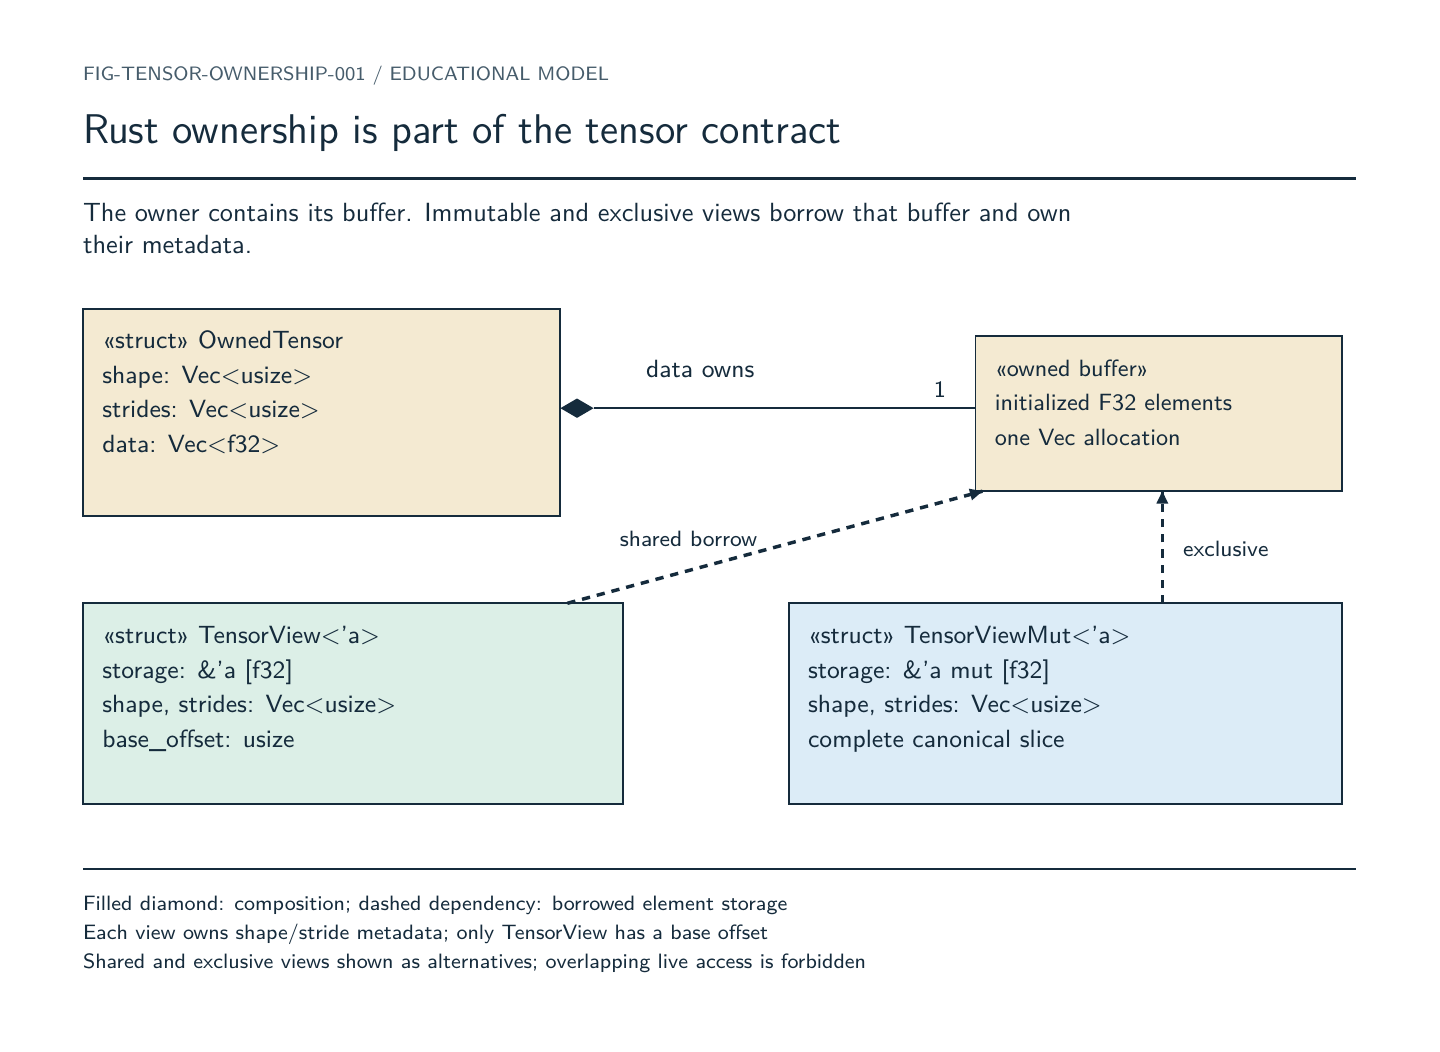
\begin{tikzpicture}[x=.5pt,y=-.5pt]
\path[use as bounding box] (0,0) rectangle (1000,720);
\path[fill=white,draw=none,line width=0.5pt] (0.0,0.0) rectangle (1000.0,720.0);
\node[inner sep=0pt,outer sep=0pt,anchor=base west,text={rgb,255:red,70;green,92;blue,107},font=\sffamily\fontsize{7.0}{8.4}\selectfont] at (40,38) {FIG-TENSOR-OWNERSHIP-001  /  EDUCATIONAL MODEL};
\node[inner sep=0pt,outer sep=0pt,anchor=base west,text={rgb,255:red,21;green,43;blue,60},font=\sffamily\fontsize{15.0}{18.0}\selectfont] at (40,84) {Rust ownership is part of the tensor contract};
\draw[fill=none,draw={rgb,255:red,21;green,43;blue,60},line width=0.75pt] (40,109) -- (960,109);
\node[inner sep=0pt,outer sep=0pt,anchor=base west,text={rgb,255:red,21;green,43;blue,60},font=\sffamily\fontsize{9.5}{11.4}\selectfont] at (40,140) {The owner contains its buffer. Immutable and exclusive views borrow that buffer and own};
\node[inner sep=0pt,outer sep=0pt,anchor=base west,text={rgb,255:red,21;green,43;blue,60},font=\sffamily\fontsize{9.5}{11.4}\selectfont] at (40,163) {their metadata.};
\path[fill={rgb,255:red,244;green,234;blue,210},draw={rgb,255:red,21;green,43;blue,60},line width=0.7pt] (40.0,203.0) rectangle (385.0,353.0);
\node[inner sep=0pt,outer sep=0pt,anchor=base west,text={rgb,255:red,21;green,43;blue,60},font=\sffamily\fontsize{9.0}{10.799999999999999}\selectfont] at (54,232) {«struct» OwnedTensor};
\node[inner sep=0pt,outer sep=0pt,anchor=base west,text={rgb,255:red,21;green,43;blue,60},font=\sffamily\fontsize{9.0}{10.799999999999999}\selectfont] at (54,257) {shape: Vec<usize>};
\node[inner sep=0pt,outer sep=0pt,anchor=base west,text={rgb,255:red,21;green,43;blue,60},font=\sffamily\fontsize{9.0}{10.799999999999999}\selectfont] at (54,282) {strides: Vec<usize>};
\node[inner sep=0pt,outer sep=0pt,anchor=base west,text={rgb,255:red,21;green,43;blue,60},font=\sffamily\fontsize{9.0}{10.799999999999999}\selectfont] at (54,307) {data: Vec<f32>};
\path[fill={rgb,255:red,244;green,234;blue,210},draw={rgb,255:red,21;green,43;blue,60},line width=0.7pt] (685.0,223.0) rectangle (950.0,335.0);
\node[inner sep=0pt,outer sep=0pt,anchor=base west,text={rgb,255:red,21;green,43;blue,60},font=\sffamily\fontsize{8.5}{10.2}\selectfont] at (699,252) {«owned buffer»};
\node[inner sep=0pt,outer sep=0pt,anchor=base west,text={rgb,255:red,21;green,43;blue,60},font=\sffamily\fontsize{8.5}{10.2}\selectfont] at (699,277) {initialized F32 elements};
\node[inner sep=0pt,outer sep=0pt,anchor=base west,text={rgb,255:red,21;green,43;blue,60},font=\sffamily\fontsize{8.5}{10.2}\selectfont] at (699,302) {one Vec allocation};
\path[fill={rgb,255:red,21;green,43;blue,60},draw=none,line width=0.5pt] (385,275) -- (397,268) -- (409,275) -- (397,282) -- cycle;
\draw[fill=none,draw={rgb,255:red,21;green,43;blue,60},line width=0.75pt] (409,275) -- (685,275);
\node[inner sep=0pt,outer sep=0pt,anchor=base west,text={rgb,255:red,21;green,43;blue,60},font=\sffamily\fontsize{9.0}{10.799999999999999}\selectfont] at (447,253) {data owns};
\node[inner sep=0pt,outer sep=0pt,anchor=base west,text={rgb,255:red,21;green,43;blue,60},font=\sffamily\fontsize{8.5}{10.2}\selectfont] at (655,267) {1};
\path[fill={rgb,255:red,220;green,239;blue,231},draw={rgb,255:red,21;green,43;blue,60},line width=0.7pt] (40.0,416.0) rectangle (430.0,561.0);
\node[inner sep=0pt,outer sep=0pt,anchor=base west,text={rgb,255:red,21;green,43;blue,60},font=\sffamily\fontsize{9.0}{10.799999999999999}\selectfont] at (54,445) {«struct» TensorView<'a>};
\node[inner sep=0pt,outer sep=0pt,anchor=base west,text={rgb,255:red,21;green,43;blue,60},font=\sffamily\fontsize{9.0}{10.799999999999999}\selectfont] at (54,470) {storage: \&'a [f32]};
\node[inner sep=0pt,outer sep=0pt,anchor=base west,text={rgb,255:red,21;green,43;blue,60},font=\sffamily\fontsize{9.0}{10.799999999999999}\selectfont] at (54,495) {shape, strides: Vec<usize>};
\node[inner sep=0pt,outer sep=0pt,anchor=base west,text={rgb,255:red,21;green,43;blue,60},font=\sffamily\fontsize{9.0}{10.799999999999999}\selectfont] at (54,520) {base\_offset: usize};
\path[fill={rgb,255:red,220;green,236;blue,247},draw={rgb,255:red,21;green,43;blue,60},line width=0.7pt] (550.0,416.0) rectangle (950.0,561.0);
\node[inner sep=0pt,outer sep=0pt,anchor=base west,text={rgb,255:red,21;green,43;blue,60},font=\sffamily\fontsize{9.0}{10.799999999999999}\selectfont] at (564,445) {«struct» TensorViewMut<'a>};
\node[inner sep=0pt,outer sep=0pt,anchor=base west,text={rgb,255:red,21;green,43;blue,60},font=\sffamily\fontsize{9.0}{10.799999999999999}\selectfont] at (564,470) {storage: \&'a mut [f32]};
\node[inner sep=0pt,outer sep=0pt,anchor=base west,text={rgb,255:red,21;green,43;blue,60},font=\sffamily\fontsize{9.0}{10.799999999999999}\selectfont] at (564,495) {shape, strides: Vec<usize>};
\node[inner sep=0pt,outer sep=0pt,anchor=base west,text={rgb,255:red,21;green,43;blue,60},font=\sffamily\fontsize{9.0}{10.799999999999999}\selectfont] at (564,520) {complete canonical slice};
\draw[fill=none,draw={rgb,255:red,21;green,43;blue,60},line width=1.25pt,dash pattern=on 3.0pt off 2.5pt] (390,416) -- (690,335);
\path[fill={rgb,255:red,21;green,43;blue,60},draw=none,line width=0.5pt] (690.00,335.00) -- (682.44,341.55) -- (680.17,333.15) -- cycle;
\node[inner sep=0pt,outer sep=0pt,anchor=base west,text={rgb,255:red,21;green,43;blue,60},font=\sffamily\fontsize{8.0}{9.6}\selectfont] at (428,375) {shared borrow};
\draw[fill=none,draw={rgb,255:red,21;green,43;blue,60},line width=1.25pt,dash pattern=on 3.0pt off 2.5pt] (820,416) -- (820,335);
\path[fill={rgb,255:red,21;green,43;blue,60},draw=none,line width=0.5pt] (820.00,335.00) -- (824.35,344.00) -- (815.65,344.00) -- cycle;
\node[inner sep=0pt,outer sep=0pt,anchor=base west,text={rgb,255:red,21;green,43;blue,60},font=\sffamily\fontsize{8.0}{9.6}\selectfont] at (835,382) {exclusive};
\draw[fill=none,draw={rgb,255:red,21;green,43;blue,60},line width=0.75pt] (40,608) -- (960,608);
\node[inner sep=0pt,outer sep=0pt,anchor=base west,text={rgb,255:red,21;green,43;blue,60},font=\sffamily\fontsize{7.5}{9.0}\selectfont] at (40,638) {Filled diamond: composition; dashed dependency: borrowed element storage};
\node[inner sep=0pt,outer sep=0pt,anchor=base west,text={rgb,255:red,21;green,43;blue,60},font=\sffamily\fontsize{7.5}{9.0}\selectfont] at (40,659) {Each view owns shape/stride metadata; only TensorView has a base offset};
\node[inner sep=0pt,outer sep=0pt,anchor=base west,text={rgb,255:red,21;green,43;blue,60},font=\sffamily\fontsize{7.5}{9.0}\selectfont] at (40,680) {Shared and exclusive views shown as alternatives; overlapping live access is forbidden};
\end{tikzpicture}
}\caption{Owned fields and borrowed slices have different relationships in the actual Rust structs.}\end{figure}

The filled diamond is UML composition: \texttt{OwnedTensor} contains a
\texttt{Vec\textless{}f32\textgreater{}} that owns initialized element
storage. The dashed dependencies are borrows of that storage, not
inheritance. Each view also owns its shape and stride vectors;
\texttt{TensorView} additionally stores a base offset.
\texttt{TensorViewMut} has no arbitrary-stride constructor and no
base-offset field because v1 limits it to the complete canonical slice.
The drawing shows the two borrowing alternatives, not permission to use
an overlapping shared view during exclusive access.

Rust lifetimes describe permitted use, not an obligation to keep a
borrow active until the end of a lexical block. The last use of a shared
view can precede a mutable borrow even when its variable remains in
scope. A surviving reference to one of its elements still counts as a
use of the same borrow. Ownership is therefore about the whole reference
chain, not merely the name of the view object.
\href{https://github.com/hermonai/inside-the-llm-engine/blob/astra-visual-rewrite/figures/generated/tensor-ownership.txt}{Text/UML
source}.

\subsection{Copy means a new owner}\label{copy-means-a-new-owner}

A copy creates new element storage. It has a separate lifetime, separate
mutation behavior, and a memory-traffic cost proportional to copied
payload. V1 names that boundary \texttt{to\_contiguous}.

{\def\LTcaptype{none} % do not increment counter
\begin{longtable}[]{@{}
  >{\raggedright\arraybackslash}p{(\linewidth - 4\tabcolsep) * \real{0.3333}}
  >{\raggedright\arraybackslash}p{(\linewidth - 4\tabcolsep) * \real{0.3333}}
  >{\raggedright\arraybackslash}p{(\linewidth - 4\tabcolsep) * \real{0.3333}}@{}}
\toprule\noalign{}
\begin{minipage}[b]{\linewidth}\raggedright
Operation
\end{minipage} & \begin{minipage}[b]{\linewidth}\raggedright
Element allocation
\end{minipage} & \begin{minipage}[b]{\linewidth}\raggedright
Element copy
\end{minipage} \\
\midrule\noalign{}
\endhead
\bottomrule\noalign{}
\endlastfoot
\texttt{from\_vec} & performed by caller; ownership moves & no \\
\texttt{zeros} & yes & zero initialization \\
\texttt{view} / \texttt{view\_mut} & no & no \\
\texttt{reshape\_view} & no & no \\
\texttt{transpose} & no & no \\
\texttt{slice\_axis} & no & no \\
\texttt{to\_contiguous} & yes & yes \\
\texttt{\seqsplit{OwnedTensor::clone}} & yes for nonempty payload & yes;
clones the owned vector \\
\texttt{\seqsplit{TensorView::clone}} & no & no; retains the storage
borrow \\
\end{longtable}
}

The distinction is shown in
\href{https://github.com/hermonai/inside-the-llm-engine/blob/astra-visual-rewrite/diagrams/tensor/view-vs-copy.txt}{view
versus copy}. Metadata allocation is intentionally separated from
element allocation in this table because model payload dominates later
memory costs.

The derived \texttt{Clone} implementation deserves explicit attention.
Cloning an owner duplicates its vectors, including the element payload;
it does not create a cheap shared handle. Cloning a view duplicates
metadata and the immutable reference, so both views still read the same
allocation. The operation's type determines which contract applies. A
review that searches only for calls named \texttt{copy} would miss the
owner's clone cost.

\begin{figure}[H]\centering\resizebox{\linewidth}{!}{% Generated from figures/generated/tensor-copy.svg; do not hand edit.
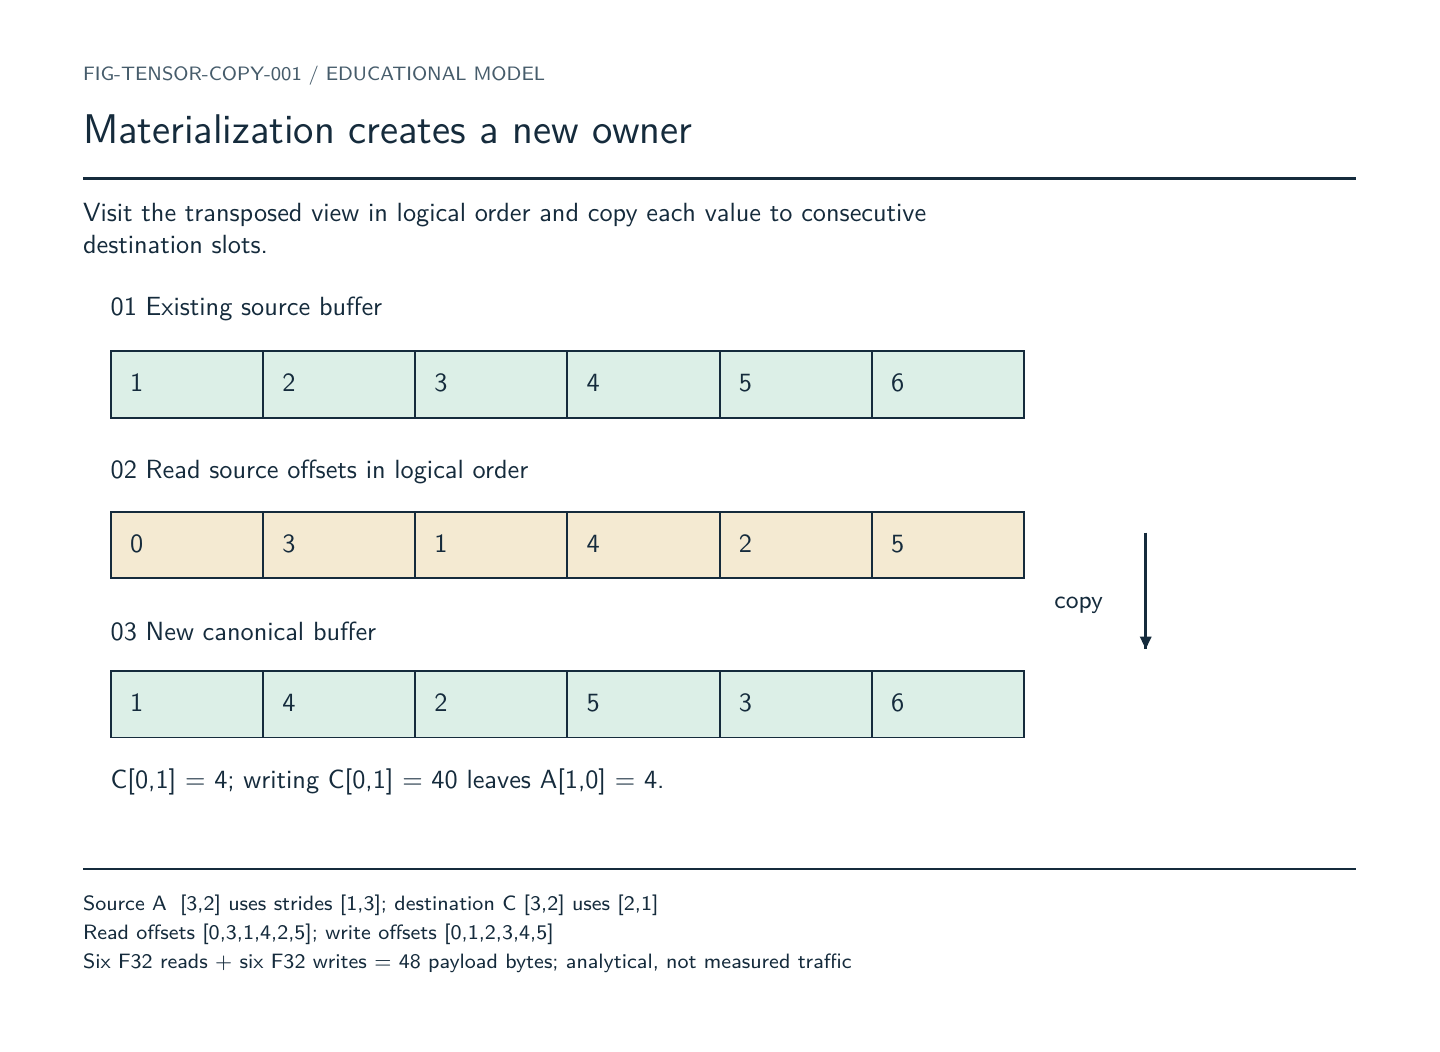
\begin{tikzpicture}[x=.5pt,y=-.5pt]
\path[use as bounding box] (0,0) rectangle (1000,720);
\path[fill=white,draw=none,line width=0.5pt] (0.0,0.0) rectangle (1000.0,720.0);
\node[inner sep=0pt,outer sep=0pt,anchor=base west,text={rgb,255:red,70;green,92;blue,107},font=\sffamily\fontsize{7.0}{8.4}\selectfont] at (40,38) {FIG-TENSOR-COPY-001  /  EDUCATIONAL MODEL};
\node[inner sep=0pt,outer sep=0pt,anchor=base west,text={rgb,255:red,21;green,43;blue,60},font=\sffamily\fontsize{15.0}{18.0}\selectfont] at (40,84) {Materialization creates a new owner};
\draw[fill=none,draw={rgb,255:red,21;green,43;blue,60},line width=0.75pt] (40,109) -- (960,109);
\node[inner sep=0pt,outer sep=0pt,anchor=base west,text={rgb,255:red,21;green,43;blue,60},font=\sffamily\fontsize{9.5}{11.4}\selectfont] at (40,140) {Visit the transposed view in logical order and copy each value to consecutive};
\node[inner sep=0pt,outer sep=0pt,anchor=base west,text={rgb,255:red,21;green,43;blue,60},font=\sffamily\fontsize{9.5}{11.4}\selectfont] at (40,163) {destination slots.};
\node[inner sep=0pt,outer sep=0pt,anchor=base west,text={rgb,255:red,21;green,43;blue,60},font=\sffamily\fontsize{9.5}{11.4}\selectfont] at (60,208) {01  Existing source buffer};
\path[fill={rgb,255:red,220;green,239;blue,231},draw={rgb,255:red,21;green,43;blue,60},line width=0.7pt] (60.0,234.0) rectangle (170.0,282.0);
\node[inner sep=0pt,outer sep=0pt,anchor=base west,text={rgb,255:red,21;green,43;blue,60},font=\sffamily\fontsize{9.5}{11.4}\selectfont] at (74,263) {1};
\path[fill={rgb,255:red,220;green,239;blue,231},draw={rgb,255:red,21;green,43;blue,60},line width=0.7pt] (170.0,234.0) rectangle (280.0,282.0);
\node[inner sep=0pt,outer sep=0pt,anchor=base west,text={rgb,255:red,21;green,43;blue,60},font=\sffamily\fontsize{9.5}{11.4}\selectfont] at (184,263) {2};
\path[fill={rgb,255:red,220;green,239;blue,231},draw={rgb,255:red,21;green,43;blue,60},line width=0.7pt] (280.0,234.0) rectangle (390.0,282.0);
\node[inner sep=0pt,outer sep=0pt,anchor=base west,text={rgb,255:red,21;green,43;blue,60},font=\sffamily\fontsize{9.5}{11.4}\selectfont] at (294,263) {3};
\path[fill={rgb,255:red,220;green,239;blue,231},draw={rgb,255:red,21;green,43;blue,60},line width=0.7pt] (390.0,234.0) rectangle (500.0,282.0);
\node[inner sep=0pt,outer sep=0pt,anchor=base west,text={rgb,255:red,21;green,43;blue,60},font=\sffamily\fontsize{9.5}{11.4}\selectfont] at (404,263) {4};
\path[fill={rgb,255:red,220;green,239;blue,231},draw={rgb,255:red,21;green,43;blue,60},line width=0.7pt] (500.0,234.0) rectangle (610.0,282.0);
\node[inner sep=0pt,outer sep=0pt,anchor=base west,text={rgb,255:red,21;green,43;blue,60},font=\sffamily\fontsize{9.5}{11.4}\selectfont] at (514,263) {5};
\path[fill={rgb,255:red,220;green,239;blue,231},draw={rgb,255:red,21;green,43;blue,60},line width=0.7pt] (610.0,234.0) rectangle (720.0,282.0);
\node[inner sep=0pt,outer sep=0pt,anchor=base west,text={rgb,255:red,21;green,43;blue,60},font=\sffamily\fontsize{9.5}{11.4}\selectfont] at (624,263) {6};
\node[inner sep=0pt,outer sep=0pt,anchor=base west,text={rgb,255:red,21;green,43;blue,60},font=\sffamily\fontsize{9.5}{11.4}\selectfont] at (60,326) {02  Read source offsets in logical order};
\path[fill={rgb,255:red,244;green,234;blue,210},draw={rgb,255:red,21;green,43;blue,60},line width=0.7pt] (60.0,350.0) rectangle (170.0,398.0);
\node[inner sep=0pt,outer sep=0pt,anchor=base west,text={rgb,255:red,21;green,43;blue,60},font=\sffamily\fontsize{9.5}{11.4}\selectfont] at (74,379) {0};
\path[fill={rgb,255:red,244;green,234;blue,210},draw={rgb,255:red,21;green,43;blue,60},line width=0.7pt] (170.0,350.0) rectangle (280.0,398.0);
\node[inner sep=0pt,outer sep=0pt,anchor=base west,text={rgb,255:red,21;green,43;blue,60},font=\sffamily\fontsize{9.5}{11.4}\selectfont] at (184,379) {3};
\path[fill={rgb,255:red,244;green,234;blue,210},draw={rgb,255:red,21;green,43;blue,60},line width=0.7pt] (280.0,350.0) rectangle (390.0,398.0);
\node[inner sep=0pt,outer sep=0pt,anchor=base west,text={rgb,255:red,21;green,43;blue,60},font=\sffamily\fontsize{9.5}{11.4}\selectfont] at (294,379) {1};
\path[fill={rgb,255:red,244;green,234;blue,210},draw={rgb,255:red,21;green,43;blue,60},line width=0.7pt] (390.0,350.0) rectangle (500.0,398.0);
\node[inner sep=0pt,outer sep=0pt,anchor=base west,text={rgb,255:red,21;green,43;blue,60},font=\sffamily\fontsize{9.5}{11.4}\selectfont] at (404,379) {4};
\path[fill={rgb,255:red,244;green,234;blue,210},draw={rgb,255:red,21;green,43;blue,60},line width=0.7pt] (500.0,350.0) rectangle (610.0,398.0);
\node[inner sep=0pt,outer sep=0pt,anchor=base west,text={rgb,255:red,21;green,43;blue,60},font=\sffamily\fontsize{9.5}{11.4}\selectfont] at (514,379) {2};
\path[fill={rgb,255:red,244;green,234;blue,210},draw={rgb,255:red,21;green,43;blue,60},line width=0.7pt] (610.0,350.0) rectangle (720.0,398.0);
\node[inner sep=0pt,outer sep=0pt,anchor=base west,text={rgb,255:red,21;green,43;blue,60},font=\sffamily\fontsize{9.5}{11.4}\selectfont] at (624,379) {5};
\draw[fill=none,draw={rgb,255:red,21;green,43;blue,60},line width=1.25pt] (808,365) -- (808,449);
\path[fill={rgb,255:red,21;green,43;blue,60},draw=none,line width=0.5pt] (808.00,449.00) -- (803.65,440.00) -- (812.35,440.00) -- cycle;
\node[inner sep=0pt,outer sep=0pt,anchor=base west,text={rgb,255:red,21;green,43;blue,60},font=\sffamily\fontsize{9.0}{10.799999999999999}\selectfont] at (742,420) {copy};
\node[inner sep=0pt,outer sep=0pt,anchor=base west,text={rgb,255:red,21;green,43;blue,60},font=\sffamily\fontsize{9.5}{11.4}\selectfont] at (60,443) {03  New canonical buffer};
\path[fill={rgb,255:red,220;green,239;blue,231},draw={rgb,255:red,21;green,43;blue,60},line width=0.7pt] (60.0,465.0) rectangle (170.0,513.0);
\node[inner sep=0pt,outer sep=0pt,anchor=base west,text={rgb,255:red,21;green,43;blue,60},font=\sffamily\fontsize{9.5}{11.4}\selectfont] at (74,494) {1};
\path[fill={rgb,255:red,220;green,239;blue,231},draw={rgb,255:red,21;green,43;blue,60},line width=0.7pt] (170.0,465.0) rectangle (280.0,513.0);
\node[inner sep=0pt,outer sep=0pt,anchor=base west,text={rgb,255:red,21;green,43;blue,60},font=\sffamily\fontsize{9.5}{11.4}\selectfont] at (184,494) {4};
\path[fill={rgb,255:red,220;green,239;blue,231},draw={rgb,255:red,21;green,43;blue,60},line width=0.7pt] (280.0,465.0) rectangle (390.0,513.0);
\node[inner sep=0pt,outer sep=0pt,anchor=base west,text={rgb,255:red,21;green,43;blue,60},font=\sffamily\fontsize{9.5}{11.4}\selectfont] at (294,494) {2};
\path[fill={rgb,255:red,220;green,239;blue,231},draw={rgb,255:red,21;green,43;blue,60},line width=0.7pt] (390.0,465.0) rectangle (500.0,513.0);
\node[inner sep=0pt,outer sep=0pt,anchor=base west,text={rgb,255:red,21;green,43;blue,60},font=\sffamily\fontsize{9.5}{11.4}\selectfont] at (404,494) {5};
\path[fill={rgb,255:red,220;green,239;blue,231},draw={rgb,255:red,21;green,43;blue,60},line width=0.7pt] (500.0,465.0) rectangle (610.0,513.0);
\node[inner sep=0pt,outer sep=0pt,anchor=base west,text={rgb,255:red,21;green,43;blue,60},font=\sffamily\fontsize{9.5}{11.4}\selectfont] at (514,494) {3};
\path[fill={rgb,255:red,220;green,239;blue,231},draw={rgb,255:red,21;green,43;blue,60},line width=0.7pt] (610.0,465.0) rectangle (720.0,513.0);
\node[inner sep=0pt,outer sep=0pt,anchor=base west,text={rgb,255:red,21;green,43;blue,60},font=\sffamily\fontsize{9.5}{11.4}\selectfont] at (624,494) {6};
\node[inner sep=0pt,outer sep=0pt,anchor=base west,text={rgb,255:red,21;green,43;blue,60},font=\sffamily\fontsize{9.5}{11.4}\selectfont] at (60,550) {C[0,1] = 4; writing C[0,1] = 40 leaves A[1,0] = 4.};
\draw[fill=none,draw={rgb,255:red,21;green,43;blue,60},line width=0.75pt] (40,608) -- (960,608);
\node[inner sep=0pt,outer sep=0pt,anchor=base west,text={rgb,255:red,21;green,43;blue,60},font=\sffamily\fontsize{7.5}{9.0}\selectfont] at (40,638) {Source Aᵀ [3,2] uses strides [1,3]; destination C [3,2] uses [2,1]};
\node[inner sep=0pt,outer sep=0pt,anchor=base west,text={rgb,255:red,21;green,43;blue,60},font=\sffamily\fontsize{7.5}{9.0}\selectfont] at (40,659) {Read offsets [0,3,1,4,2,5]; write offsets [0,1,2,3,4,5]};
\node[inner sep=0pt,outer sep=0pt,anchor=base west,text={rgb,255:red,21;green,43;blue,60},font=\sffamily\fontsize{7.5}{9.0}\selectfont] at (40,680) {Six F32 reads + six F32 writes = 48 payload bytes; analytical, not measured traffic};
\end{tikzpicture}
}\caption{Materialization reads a strided logical sequence and writes a new canonical allocation.}\end{figure}

For the transposed six-value view, \texttt{to\_contiguous} reads source
offsets \texttt{{[}0,3,1,4,2,5{]}} and writes destination offsets
\texttt{{[}0,1,2,3,4,5{]}}. The new physical buffer is
\texttt{{[}1,4,2,5,3,6{]}}. Its logical values equal the transposed
source even though its physical order and owner differ. Changing the
copy's \texttt{{[}0,1{]}} from 4 to 40 must leave the original matrix's
\texttt{{[}1,0{]}} equal to 4.

For \(N\) F32 elements, the analytical payload movement of this explicit
copy is

\[
Q_{\mathrm{copy,payload}}=N\times4+N\times4=8N\quad[\mathrm{bytes}].
\]

Here the two terms count logical element reads and writes. For our
example, \(N=6\) gives 48 payload bytes. This is not a measurement of
DRAM traffic: cache lines, write allocation, metadata, allocator
bookkeeping and validation are outside the count. The function also
allocates coordinate vectors while enumerating logical indices. Its
clarity-first implementation is not a promise of a production memcpy
cost.
\href{https://github.com/hermonai/inside-the-llm-engine/blob/astra-visual-rewrite/figures/generated/tensor-copy.txt}{Text
sequence}.

\begin{quote}
\textbf{FIRST PRINCIPLE} Allocation and copying must be visible
operations. A convenient-looking metadata transform must not secretly
materialize a model-sized payload.
\end{quote}

\subsection{Reshape changes grouping}\label{reshape-changes-grouping}

A no-copy reshape changes how one contiguous sequence is grouped into
axes. The six physical values \texttt{1,2,3,4,5,6} can be viewed as
\texttt{{[}2,3{]}}, \texttt{{[}3,2{]}}, \texttt{{[}6{]}}, or
\texttt{{[}1,6{]}}. Logical row-major iteration remains physical offsets
\texttt{0,1,2,3,4,5}.

V1's \texttt{reshape\_view} requires two proofs:

\begin{enumerate}
\def\labelenumi{\arabic{enumi}.}
\tightlist
\item
  The source has exact canonical row-major strides.
\item
  The requested checked element count equals the current count.
\end{enumerate}

It then derives canonical strides for the new shape and borrows the same
storage. Shape \texttt{{[}4,2{]}} fails because it asks six values to
become eight. A non-contiguous transpose fails with
\texttt{NonContiguous}; v1 does not copy as a fallback. The canonical
\href{https://github.com/hermonai/inside-the-llm-engine/blob/astra-visual-rewrite/diagrams/tensor/reshape-view.txt}{reshape
view} makes the shared owner and changed grouping explicit.

\begin{figure}[H]\centering\resizebox{\linewidth}{!}{% Generated from figures/generated/tensor-reshape.svg; do not hand edit.
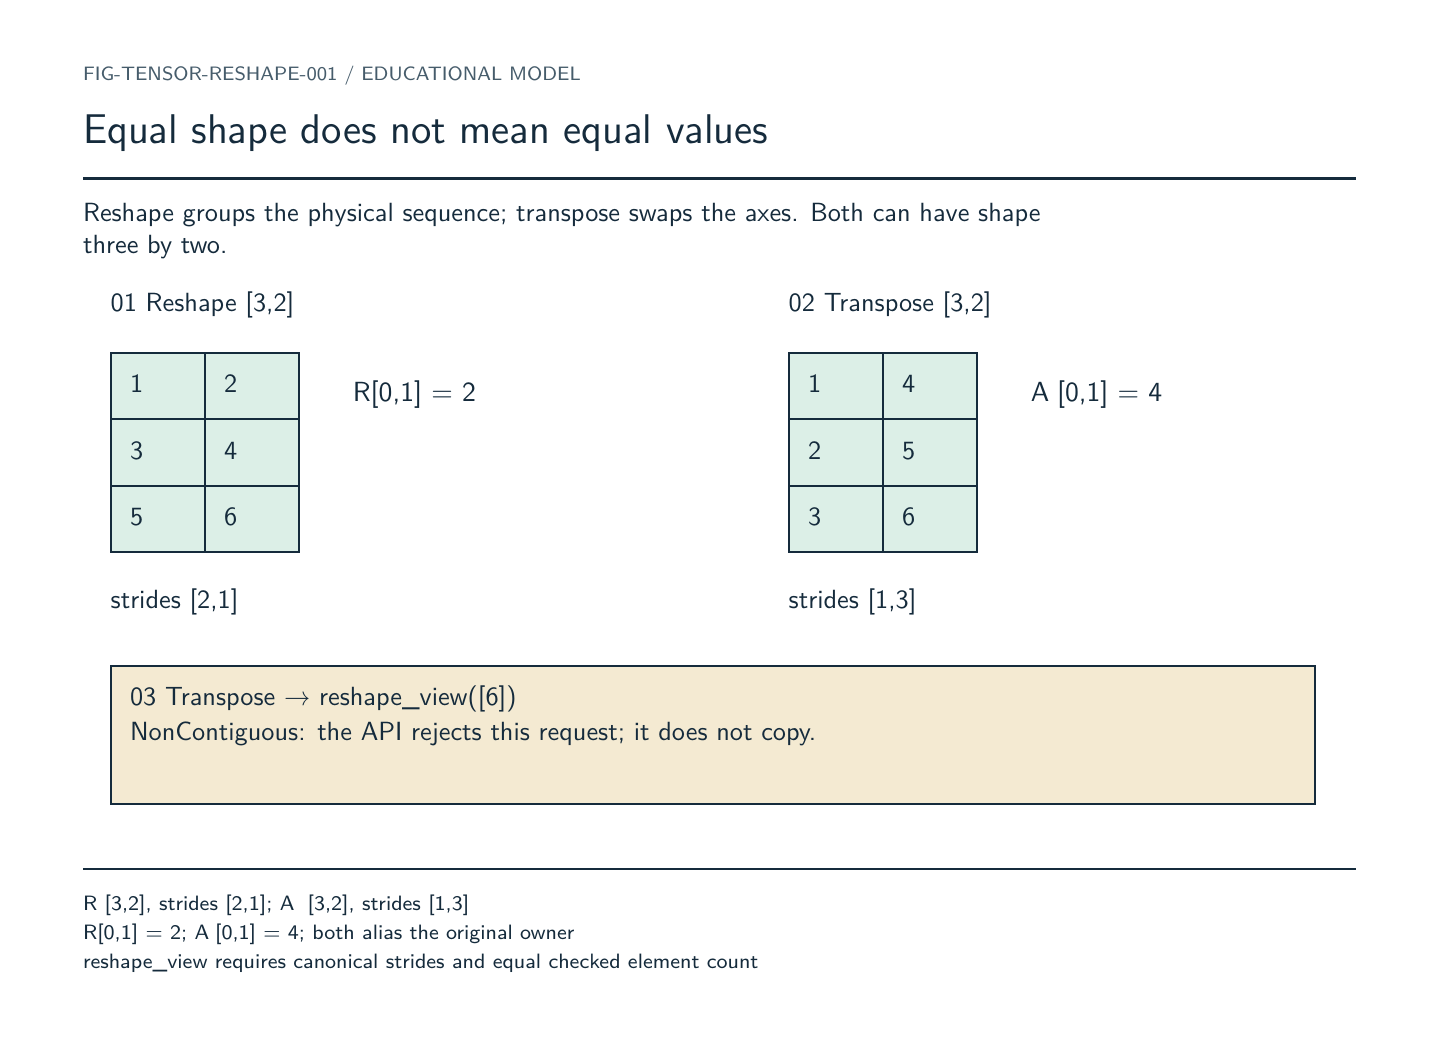
\begin{tikzpicture}[x=.5pt,y=-.5pt]
\path[use as bounding box] (0,0) rectangle (1000,720);
\path[fill=white,draw=none,line width=0.5pt] (0.0,0.0) rectangle (1000.0,720.0);
\node[inner sep=0pt,outer sep=0pt,anchor=base west,text={rgb,255:red,70;green,92;blue,107},font=\sffamily\fontsize{7.0}{8.4}\selectfont] at (40,38) {FIG-TENSOR-RESHAPE-001  /  EDUCATIONAL MODEL};
\node[inner sep=0pt,outer sep=0pt,anchor=base west,text={rgb,255:red,21;green,43;blue,60},font=\sffamily\fontsize{15.0}{18.0}\selectfont] at (40,84) {Equal shape does not mean equal values};
\draw[fill=none,draw={rgb,255:red,21;green,43;blue,60},line width=0.75pt] (40,109) -- (960,109);
\node[inner sep=0pt,outer sep=0pt,anchor=base west,text={rgb,255:red,21;green,43;blue,60},font=\sffamily\fontsize{9.5}{11.4}\selectfont] at (40,140) {Reshape groups the physical sequence; transpose swaps the axes. Both can have shape};
\node[inner sep=0pt,outer sep=0pt,anchor=base west,text={rgb,255:red,21;green,43;blue,60},font=\sffamily\fontsize{9.5}{11.4}\selectfont] at (40,163) {three by two.};
\node[inner sep=0pt,outer sep=0pt,anchor=base west,text={rgb,255:red,21;green,43;blue,60},font=\sffamily\fontsize{9.5}{11.4}\selectfont] at (60,205) {01  Reshape [3,2]};
\path[fill={rgb,255:red,220;green,239;blue,231},draw={rgb,255:red,21;green,43;blue,60},line width=0.7pt] (60.0,235.0) rectangle (128.0,283.0);
\node[inner sep=0pt,outer sep=0pt,anchor=base west,text={rgb,255:red,21;green,43;blue,60},font=\sffamily\fontsize{9.5}{11.4}\selectfont] at (74,264) {1};
\path[fill={rgb,255:red,220;green,239;blue,231},draw={rgb,255:red,21;green,43;blue,60},line width=0.7pt] (128.0,235.0) rectangle (196.0,283.0);
\node[inner sep=0pt,outer sep=0pt,anchor=base west,text={rgb,255:red,21;green,43;blue,60},font=\sffamily\fontsize{9.5}{11.4}\selectfont] at (142,264) {2};
\path[fill={rgb,255:red,220;green,239;blue,231},draw={rgb,255:red,21;green,43;blue,60},line width=0.7pt] (60.0,283.0) rectangle (128.0,331.0);
\node[inner sep=0pt,outer sep=0pt,anchor=base west,text={rgb,255:red,21;green,43;blue,60},font=\sffamily\fontsize{9.5}{11.4}\selectfont] at (74,312) {3};
\path[fill={rgb,255:red,220;green,239;blue,231},draw={rgb,255:red,21;green,43;blue,60},line width=0.7pt] (128.0,283.0) rectangle (196.0,331.0);
\node[inner sep=0pt,outer sep=0pt,anchor=base west,text={rgb,255:red,21;green,43;blue,60},font=\sffamily\fontsize{9.5}{11.4}\selectfont] at (142,312) {4};
\path[fill={rgb,255:red,220;green,239;blue,231},draw={rgb,255:red,21;green,43;blue,60},line width=0.7pt] (60.0,331.0) rectangle (128.0,379.0);
\node[inner sep=0pt,outer sep=0pt,anchor=base west,text={rgb,255:red,21;green,43;blue,60},font=\sffamily\fontsize{9.5}{11.4}\selectfont] at (74,360) {5};
\path[fill={rgb,255:red,220;green,239;blue,231},draw={rgb,255:red,21;green,43;blue,60},line width=0.7pt] (128.0,331.0) rectangle (196.0,379.0);
\node[inner sep=0pt,outer sep=0pt,anchor=base west,text={rgb,255:red,21;green,43;blue,60},font=\sffamily\fontsize{9.5}{11.4}\selectfont] at (142,360) {6};
\node[inner sep=0pt,outer sep=0pt,anchor=base west,text={rgb,255:red,21;green,43;blue,60},font=\sffamily\fontsize{9.5}{11.4}\selectfont] at (550,205) {02  Transpose [3,2]};
\path[fill={rgb,255:red,220;green,239;blue,231},draw={rgb,255:red,21;green,43;blue,60},line width=0.7pt] (550.0,235.0) rectangle (618.0,283.0);
\node[inner sep=0pt,outer sep=0pt,anchor=base west,text={rgb,255:red,21;green,43;blue,60},font=\sffamily\fontsize{9.5}{11.4}\selectfont] at (564,264) {1};
\path[fill={rgb,255:red,220;green,239;blue,231},draw={rgb,255:red,21;green,43;blue,60},line width=0.7pt] (618.0,235.0) rectangle (686.0,283.0);
\node[inner sep=0pt,outer sep=0pt,anchor=base west,text={rgb,255:red,21;green,43;blue,60},font=\sffamily\fontsize{9.5}{11.4}\selectfont] at (632,264) {4};
\path[fill={rgb,255:red,220;green,239;blue,231},draw={rgb,255:red,21;green,43;blue,60},line width=0.7pt] (550.0,283.0) rectangle (618.0,331.0);
\node[inner sep=0pt,outer sep=0pt,anchor=base west,text={rgb,255:red,21;green,43;blue,60},font=\sffamily\fontsize{9.5}{11.4}\selectfont] at (564,312) {2};
\path[fill={rgb,255:red,220;green,239;blue,231},draw={rgb,255:red,21;green,43;blue,60},line width=0.7pt] (618.0,283.0) rectangle (686.0,331.0);
\node[inner sep=0pt,outer sep=0pt,anchor=base west,text={rgb,255:red,21;green,43;blue,60},font=\sffamily\fontsize{9.5}{11.4}\selectfont] at (632,312) {5};
\path[fill={rgb,255:red,220;green,239;blue,231},draw={rgb,255:red,21;green,43;blue,60},line width=0.7pt] (550.0,331.0) rectangle (618.0,379.0);
\node[inner sep=0pt,outer sep=0pt,anchor=base west,text={rgb,255:red,21;green,43;blue,60},font=\sffamily\fontsize{9.5}{11.4}\selectfont] at (564,360) {3};
\path[fill={rgb,255:red,220;green,239;blue,231},draw={rgb,255:red,21;green,43;blue,60},line width=0.7pt] (618.0,331.0) rectangle (686.0,379.0);
\node[inner sep=0pt,outer sep=0pt,anchor=base west,text={rgb,255:red,21;green,43;blue,60},font=\sffamily\fontsize{9.5}{11.4}\selectfont] at (632,360) {6};
\node[inner sep=0pt,outer sep=0pt,anchor=base west,text={rgb,255:red,21;green,43;blue,60},font=\sffamily\fontsize{10.0}{12.0}\selectfont] at (235,270) {R[0,1] = 2};
\node[inner sep=0pt,outer sep=0pt,anchor=base west,text={rgb,255:red,21;green,43;blue,60},font=\sffamily\fontsize{10.0}{12.0}\selectfont] at (725,270) {Aᵀ[0,1] = 4};
\node[inner sep=0pt,outer sep=0pt,anchor=base west,text={rgb,255:red,21;green,43;blue,60},font=\sffamily\fontsize{9.5}{11.4}\selectfont] at (60,420) {strides [2,1]};
\node[inner sep=0pt,outer sep=0pt,anchor=base west,text={rgb,255:red,21;green,43;blue,60},font=\sffamily\fontsize{9.5}{11.4}\selectfont] at (550,420) {strides [1,3]};
\path[fill={rgb,255:red,244;green,234;blue,210},draw={rgb,255:red,21;green,43;blue,60},line width=0.7pt] (60.0,461.0) rectangle (930.0,561.0);
\node[inner sep=0pt,outer sep=0pt,anchor=base west,text={rgb,255:red,21;green,43;blue,60},font=\sffamily\fontsize{9.5}{11.4}\selectfont] at (74,490) {03  Transpose → reshape\_view([6])};
\node[inner sep=0pt,outer sep=0pt,anchor=base west,text={rgb,255:red,21;green,43;blue,60},font=\sffamily\fontsize{9.5}{11.4}\selectfont] at (74,515) {NonContiguous: the API rejects this request; it does not copy.};
\draw[fill=none,draw={rgb,255:red,21;green,43;blue,60},line width=0.75pt] (40,608) -- (960,608);
\node[inner sep=0pt,outer sep=0pt,anchor=base west,text={rgb,255:red,21;green,43;blue,60},font=\sffamily\fontsize{7.5}{9.0}\selectfont] at (40,638) {R [3,2], strides [2,1]; Aᵀ [3,2], strides [1,3]};
\node[inner sep=0pt,outer sep=0pt,anchor=base west,text={rgb,255:red,21;green,43;blue,60},font=\sffamily\fontsize{7.5}{9.0}\selectfont] at (40,659) {R[0,1] = 2; Aᵀ[0,1] = 4; both alias the original owner};
\node[inner sep=0pt,outer sep=0pt,anchor=base west,text={rgb,255:red,21;green,43;blue,60},font=\sffamily\fontsize{7.5}{9.0}\selectfont] at (40,680) {reshape\_view requires canonical strides and equal checked element count};
\end{tikzpicture}
}\caption{Reshape and transpose both produce three-by-two views but disagree at the same coordinate.}\end{figure}

Let \(\mathbf{R}\) be the \texttt{{[}3,2{]}} reshape of our original
owner. Its strides are \texttt{{[}2,1{]}}, and \(R_{0,1}=2\). The
transpose has shape \texttt{{[}3,2{]}} too, but its strides are
\texttt{{[}1,3{]}}, so \((A^{\mathsf T})_{0,1}=4\). Both results are
valid aliases. Checking only the shape would not reveal their different
mathematical values. An operator contract must therefore state whether
it honors general strides, requires canonical input, or performs an
explicit conversion.

PyTorch's \texttt{view} supports a broader compatibility condition based
on adjacent stride relationships, while \texttt{reshape} may choose a
view or copy. That is useful framework behavior. It is too implicit for
our first substrate, where the method name itself should reveal
allocation.

\subsection{Transpose changes logical
movement}\label{transpose-changes-logical-movement}

Transpose is not reshape. For the original \texttt{{[}2,3{]}} matrix:

\begin{center}\begin{adjustbox}{max width=\linewidth}% Legacy topology preserved as native vectors and typeset labels.
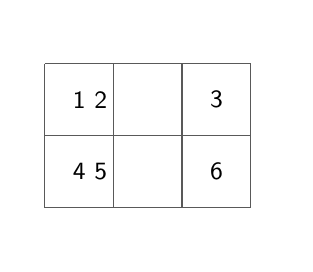
\begin{tikzpicture}[x=6.2pt,y=-13pt,draw=black!65,line width=.45pt]
\path[use as bounding box] (-1,-1) rectangle (14,5);
\draw (0,0) -- (0.5,0);
\draw (0,0) -- (0,0.5);
\draw (1,0) -- (0.5,0);
\draw (1,0) -- (1.5,0);
\draw (2,0) -- (1.5,0);
\draw (2,0) -- (2.5,0);
\draw (3,0) -- (2.5,0);
\draw (3,0) -- (3.5,0);
\draw (4,0) -- (3.5,0);
\draw (4,0) -- (4.5,0);
\draw (4,0) -- (4,0.5);
\draw (5,0) -- (4.5,0);
\draw (5,0) -- (5.5,0);
\draw (6,0) -- (5.5,0);
\draw (6,0) -- (6.5,0);
\draw (7,0) -- (6.5,0);
\draw (7,0) -- (7.5,0);
\draw (8,0) -- (7.5,0);
\draw (8,0) -- (8.5,0);
\draw (8,0) -- (8,0.5);
\draw (9,0) -- (8.5,0);
\draw (9,0) -- (9.5,0);
\draw (10,0) -- (9.5,0);
\draw (10,0) -- (10.5,0);
\draw (11,0) -- (10.5,0);
\draw (11,0) -- (11.5,0);
\draw (12,0) -- (11.5,0);
\draw (12,0) -- (12,0.5);
\draw (0,1) -- (0,0.5);
\draw (0,1) -- (0,1.5);
\draw (4,1) -- (4,0.5);
\draw (4,1) -- (4,1.5);
\draw (8,1) -- (8,0.5);
\draw (8,1) -- (8,1.5);
\draw (12,1) -- (12,0.5);
\draw (12,1) -- (12,1.5);
\node[anchor=west,inner sep=0pt,font=\sffamily\fontsize{9}{11}\selectfont] at (1.6,1) {\begin{adjustbox}{max width=31.0pt}1   2\end{adjustbox}};
\node[anchor=west,inner sep=0pt,font=\sffamily\fontsize{9}{11}\selectfont] at (9.6,1) {\begin{adjustbox}{max width=6.2pt}3\end{adjustbox}};
\draw (0,2) -- (0,1.5);
\draw (0,2) -- (0.5,2);
\draw (0,2) -- (0,2.5);
\draw (1,2) -- (0.5,2);
\draw (1,2) -- (1.5,2);
\draw (2,2) -- (1.5,2);
\draw (2,2) -- (2.5,2);
\draw (3,2) -- (2.5,2);
\draw (3,2) -- (3.5,2);
\draw (4,2) -- (3.5,2);
\draw (4,2) -- (4.5,2);
\draw (4,2) -- (4,1.5);
\draw (4,2) -- (4,2.5);
\draw (5,2) -- (4.5,2);
\draw (5,2) -- (5.5,2);
\draw (6,2) -- (5.5,2);
\draw (6,2) -- (6.5,2);
\draw (7,2) -- (6.5,2);
\draw (7,2) -- (7.5,2);
\draw (8,2) -- (7.5,2);
\draw (8,2) -- (8.5,2);
\draw (8,2) -- (8,1.5);
\draw (8,2) -- (8,2.5);
\draw (9,2) -- (8.5,2);
\draw (9,2) -- (9.5,2);
\draw (10,2) -- (9.5,2);
\draw (10,2) -- (10.5,2);
\draw (11,2) -- (10.5,2);
\draw (11,2) -- (11.5,2);
\draw (12,2) -- (12,1.5);
\draw (12,2) -- (11.5,2);
\draw (12,2) -- (12,2.5);
\draw (0,3) -- (0,2.5);
\draw (0,3) -- (0,3.5);
\draw (4,3) -- (4,2.5);
\draw (4,3) -- (4,3.5);
\draw (8,3) -- (8,2.5);
\draw (8,3) -- (8,3.5);
\draw (12,3) -- (12,2.5);
\draw (12,3) -- (12,3.5);
\node[anchor=west,inner sep=0pt,font=\sffamily\fontsize{9}{11}\selectfont] at (1.6,3) {\begin{adjustbox}{max width=31.0pt}4   5\end{adjustbox}};
\node[anchor=west,inner sep=0pt,font=\sffamily\fontsize{9}{11}\selectfont] at (9.6,3) {\begin{adjustbox}{max width=6.2pt}6\end{adjustbox}};
\draw (0,4) -- (0.5,4);
\draw (0,4) -- (0,3.5);
\draw (1,4) -- (0.5,4);
\draw (1,4) -- (1.5,4);
\draw (2,4) -- (1.5,4);
\draw (2,4) -- (2.5,4);
\draw (3,4) -- (2.5,4);
\draw (3,4) -- (3.5,4);
\draw (4,4) -- (3.5,4);
\draw (4,4) -- (4.5,4);
\draw (4,4) -- (4,3.5);
\draw (5,4) -- (4.5,4);
\draw (5,4) -- (5.5,4);
\draw (6,4) -- (5.5,4);
\draw (6,4) -- (6.5,4);
\draw (7,4) -- (6.5,4);
\draw (7,4) -- (7.5,4);
\draw (8,4) -- (7.5,4);
\draw (8,4) -- (8.5,4);
\draw (8,4) -- (8,3.5);
\draw (9,4) -- (8.5,4);
\draw (9,4) -- (9.5,4);
\draw (10,4) -- (9.5,4);
\draw (10,4) -- (10.5,4);
\draw (11,4) -- (10.5,4);
\draw (11,4) -- (11.5,4);
\draw (12,4) -- (11.5,4);
\draw (12,4) -- (12,3.5);
\end{tikzpicture}
\end{adjustbox}\end{center}

the rank-2 transpose is logically:

\begin{center}\begin{adjustbox}{max width=\linewidth}% Legacy topology preserved as native vectors and typeset labels.
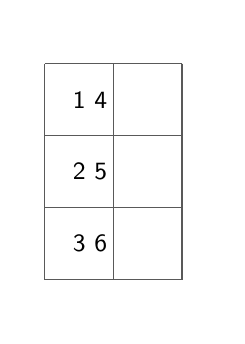
\begin{tikzpicture}[x=6.2pt,y=-13pt,draw=black!65,line width=.45pt]
\path[use as bounding box] (-1,-1) rectangle (10,7);
\draw (0,0) -- (0.5,0);
\draw (0,0) -- (0,0.5);
\draw (1,0) -- (0.5,0);
\draw (1,0) -- (1.5,0);
\draw (2,0) -- (1.5,0);
\draw (2,0) -- (2.5,0);
\draw (3,0) -- (2.5,0);
\draw (3,0) -- (3.5,0);
\draw (4,0) -- (3.5,0);
\draw (4,0) -- (4.5,0);
\draw (4,0) -- (4,0.5);
\draw (5,0) -- (4.5,0);
\draw (5,0) -- (5.5,0);
\draw (6,0) -- (5.5,0);
\draw (6,0) -- (6.5,0);
\draw (7,0) -- (6.5,0);
\draw (7,0) -- (7.5,0);
\draw (8,0) -- (7.5,0);
\draw (8,0) -- (8,0.5);
\draw (0,1) -- (0,0.5);
\draw (0,1) -- (0,1.5);
\draw (4,1) -- (4,0.5);
\draw (4,1) -- (4,1.5);
\draw (8,1) -- (8,0.5);
\draw (8,1) -- (8,1.5);
\node[anchor=west,inner sep=0pt,font=\sffamily\fontsize{9}{11}\selectfont] at (1.6,1) {\begin{adjustbox}{max width=31.0pt}1   4\end{adjustbox}};
\draw (0,2) -- (0,1.5);
\draw (0,2) -- (0.5,2);
\draw (0,2) -- (0,2.5);
\draw (1,2) -- (0.5,2);
\draw (1,2) -- (1.5,2);
\draw (2,2) -- (1.5,2);
\draw (2,2) -- (2.5,2);
\draw (3,2) -- (2.5,2);
\draw (3,2) -- (3.5,2);
\draw (4,2) -- (3.5,2);
\draw (4,2) -- (4.5,2);
\draw (4,2) -- (4,1.5);
\draw (4,2) -- (4,2.5);
\draw (5,2) -- (4.5,2);
\draw (5,2) -- (5.5,2);
\draw (6,2) -- (5.5,2);
\draw (6,2) -- (6.5,2);
\draw (7,2) -- (6.5,2);
\draw (7,2) -- (7.5,2);
\draw (8,2) -- (8,1.5);
\draw (8,2) -- (7.5,2);
\draw (8,2) -- (8,2.5);
\draw (0,3) -- (0,2.5);
\draw (0,3) -- (0,3.5);
\draw (4,3) -- (4,2.5);
\draw (4,3) -- (4,3.5);
\draw (8,3) -- (8,2.5);
\draw (8,3) -- (8,3.5);
\node[anchor=west,inner sep=0pt,font=\sffamily\fontsize{9}{11}\selectfont] at (1.6,3) {\begin{adjustbox}{max width=31.0pt}2   5\end{adjustbox}};
\draw (0,4) -- (0,3.5);
\draw (0,4) -- (0.5,4);
\draw (0,4) -- (0,4.5);
\draw (1,4) -- (0.5,4);
\draw (1,4) -- (1.5,4);
\draw (2,4) -- (1.5,4);
\draw (2,4) -- (2.5,4);
\draw (3,4) -- (2.5,4);
\draw (3,4) -- (3.5,4);
\draw (4,4) -- (3.5,4);
\draw (4,4) -- (4.5,4);
\draw (4,4) -- (4,3.5);
\draw (4,4) -- (4,4.5);
\draw (5,4) -- (4.5,4);
\draw (5,4) -- (5.5,4);
\draw (6,4) -- (5.5,4);
\draw (6,4) -- (6.5,4);
\draw (7,4) -- (6.5,4);
\draw (7,4) -- (7.5,4);
\draw (8,4) -- (8,3.5);
\draw (8,4) -- (7.5,4);
\draw (8,4) -- (8,4.5);
\draw (0,5) -- (0,4.5);
\draw (0,5) -- (0,5.5);
\draw (4,5) -- (4,4.5);
\draw (4,5) -- (4,5.5);
\draw (8,5) -- (8,4.5);
\draw (8,5) -- (8,5.5);
\node[anchor=west,inner sep=0pt,font=\sffamily\fontsize{9}{11}\selectfont] at (1.6,5) {\begin{adjustbox}{max width=31.0pt}3   6\end{adjustbox}};
\draw (0,6) -- (0.5,6);
\draw (0,6) -- (0,5.5);
\draw (1,6) -- (0.5,6);
\draw (1,6) -- (1.5,6);
\draw (2,6) -- (1.5,6);
\draw (2,6) -- (2.5,6);
\draw (3,6) -- (2.5,6);
\draw (3,6) -- (3.5,6);
\draw (4,6) -- (3.5,6);
\draw (4,6) -- (4.5,6);
\draw (4,6) -- (4,5.5);
\draw (5,6) -- (4.5,6);
\draw (5,6) -- (5.5,6);
\draw (6,6) -- (5.5,6);
\draw (6,6) -- (6.5,6);
\draw (7,6) -- (6.5,6);
\draw (7,6) -- (7.5,6);
\draw (8,6) -- (7.5,6);
\draw (8,6) -- (8,5.5);
\end{tikzpicture}
\end{adjustbox}\end{center}

No bytes move. Shape \texttt{{[}2,3{]}} becomes \texttt{{[}3,2{]}};
strides \texttt{{[}3,1{]}} become \texttt{{[}1,3{]}}. Logical row-major
traversal now visits physical offsets \texttt{{[}0,3,1,4,2,5{]}}. The
canonical
\href{https://github.com/hermonai/inside-the-llm-engine/blob/astra-visual-rewrite/diagrams/tensor/transpose-view.txt}{transpose
view} shows both interpretations over one owner.

\begin{figure}[H]\centering\resizebox{\linewidth}{!}{% Generated from figures/generated/tensor-transpose.svg; do not hand edit.
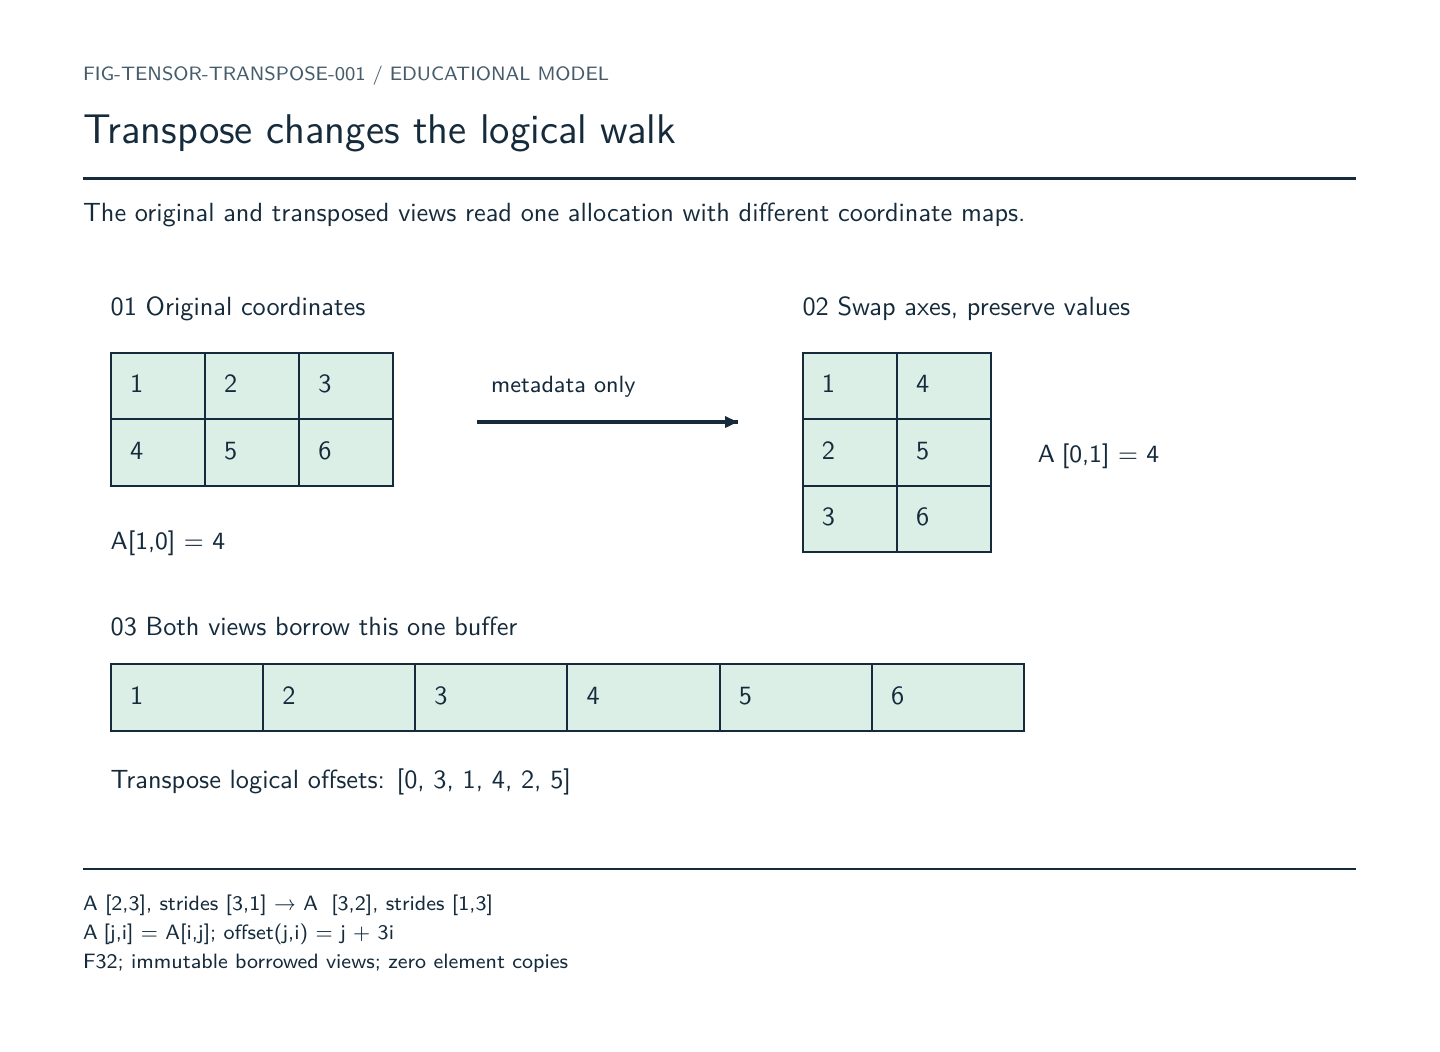
\begin{tikzpicture}[x=.5pt,y=-.5pt]
\path[use as bounding box] (0,0) rectangle (1000,720);
\path[fill=white,draw=none,line width=0.5pt] (0.0,0.0) rectangle (1000.0,720.0);
\node[inner sep=0pt,outer sep=0pt,anchor=base west,text={rgb,255:red,70;green,92;blue,107},font=\sffamily\fontsize{7.0}{8.4}\selectfont] at (40,38) {FIG-TENSOR-TRANSPOSE-001  /  EDUCATIONAL MODEL};
\node[inner sep=0pt,outer sep=0pt,anchor=base west,text={rgb,255:red,21;green,43;blue,60},font=\sffamily\fontsize{15.0}{18.0}\selectfont] at (40,84) {Transpose changes the logical walk};
\draw[fill=none,draw={rgb,255:red,21;green,43;blue,60},line width=0.75pt] (40,109) -- (960,109);
\node[inner sep=0pt,outer sep=0pt,anchor=base west,text={rgb,255:red,21;green,43;blue,60},font=\sffamily\fontsize{9.5}{11.4}\selectfont] at (40,140) {The original and transposed views read one allocation with different coordinate maps.};
\node[inner sep=0pt,outer sep=0pt,anchor=base west,text={rgb,255:red,21;green,43;blue,60},font=\sffamily\fontsize{9.5}{11.4}\selectfont] at (60,208) {01  Original coordinates};
\path[fill={rgb,255:red,220;green,239;blue,231},draw={rgb,255:red,21;green,43;blue,60},line width=0.7pt] (60.0,235.0) rectangle (128.0,283.0);
\node[inner sep=0pt,outer sep=0pt,anchor=base west,text={rgb,255:red,21;green,43;blue,60},font=\sffamily\fontsize{9.5}{11.4}\selectfont] at (74,264) {1};
\path[fill={rgb,255:red,220;green,239;blue,231},draw={rgb,255:red,21;green,43;blue,60},line width=0.7pt] (128.0,235.0) rectangle (196.0,283.0);
\node[inner sep=0pt,outer sep=0pt,anchor=base west,text={rgb,255:red,21;green,43;blue,60},font=\sffamily\fontsize{9.5}{11.4}\selectfont] at (142,264) {2};
\path[fill={rgb,255:red,220;green,239;blue,231},draw={rgb,255:red,21;green,43;blue,60},line width=0.7pt] (196.0,235.0) rectangle (264.0,283.0);
\node[inner sep=0pt,outer sep=0pt,anchor=base west,text={rgb,255:red,21;green,43;blue,60},font=\sffamily\fontsize{9.5}{11.4}\selectfont] at (210,264) {3};
\path[fill={rgb,255:red,220;green,239;blue,231},draw={rgb,255:red,21;green,43;blue,60},line width=0.7pt] (60.0,283.0) rectangle (128.0,331.0);
\node[inner sep=0pt,outer sep=0pt,anchor=base west,text={rgb,255:red,21;green,43;blue,60},font=\sffamily\fontsize{9.5}{11.4}\selectfont] at (74,312) {4};
\path[fill={rgb,255:red,220;green,239;blue,231},draw={rgb,255:red,21;green,43;blue,60},line width=0.7pt] (128.0,283.0) rectangle (196.0,331.0);
\node[inner sep=0pt,outer sep=0pt,anchor=base west,text={rgb,255:red,21;green,43;blue,60},font=\sffamily\fontsize{9.5}{11.4}\selectfont] at (142,312) {5};
\path[fill={rgb,255:red,220;green,239;blue,231},draw={rgb,255:red,21;green,43;blue,60},line width=0.7pt] (196.0,283.0) rectangle (264.0,331.0);
\node[inner sep=0pt,outer sep=0pt,anchor=base west,text={rgb,255:red,21;green,43;blue,60},font=\sffamily\fontsize{9.5}{11.4}\selectfont] at (210,312) {6};
\node[inner sep=0pt,outer sep=0pt,anchor=base west,text={rgb,255:red,21;green,43;blue,60},font=\sffamily\fontsize{9.5}{11.4}\selectfont] at (560,208) {02  Swap axes, preserve values};
\path[fill={rgb,255:red,220;green,239;blue,231},draw={rgb,255:red,21;green,43;blue,60},line width=0.7pt] (560.0,235.0) rectangle (628.0,283.0);
\node[inner sep=0pt,outer sep=0pt,anchor=base west,text={rgb,255:red,21;green,43;blue,60},font=\sffamily\fontsize{9.5}{11.4}\selectfont] at (574,264) {1};
\path[fill={rgb,255:red,220;green,239;blue,231},draw={rgb,255:red,21;green,43;blue,60},line width=0.7pt] (628.0,235.0) rectangle (696.0,283.0);
\node[inner sep=0pt,outer sep=0pt,anchor=base west,text={rgb,255:red,21;green,43;blue,60},font=\sffamily\fontsize{9.5}{11.4}\selectfont] at (642,264) {4};
\path[fill={rgb,255:red,220;green,239;blue,231},draw={rgb,255:red,21;green,43;blue,60},line width=0.7pt] (560.0,283.0) rectangle (628.0,331.0);
\node[inner sep=0pt,outer sep=0pt,anchor=base west,text={rgb,255:red,21;green,43;blue,60},font=\sffamily\fontsize{9.5}{11.4}\selectfont] at (574,312) {2};
\path[fill={rgb,255:red,220;green,239;blue,231},draw={rgb,255:red,21;green,43;blue,60},line width=0.7pt] (628.0,283.0) rectangle (696.0,331.0);
\node[inner sep=0pt,outer sep=0pt,anchor=base west,text={rgb,255:red,21;green,43;blue,60},font=\sffamily\fontsize{9.5}{11.4}\selectfont] at (642,312) {5};
\path[fill={rgb,255:red,220;green,239;blue,231},draw={rgb,255:red,21;green,43;blue,60},line width=0.7pt] (560.0,331.0) rectangle (628.0,379.0);
\node[inner sep=0pt,outer sep=0pt,anchor=base west,text={rgb,255:red,21;green,43;blue,60},font=\sffamily\fontsize{9.5}{11.4}\selectfont] at (574,360) {3};
\path[fill={rgb,255:red,220;green,239;blue,231},draw={rgb,255:red,21;green,43;blue,60},line width=0.7pt] (628.0,331.0) rectangle (696.0,379.0);
\node[inner sep=0pt,outer sep=0pt,anchor=base west,text={rgb,255:red,21;green,43;blue,60},font=\sffamily\fontsize{9.5}{11.4}\selectfont] at (642,360) {6};
\draw[fill=none,draw={rgb,255:red,21;green,43;blue,60},line width=1.25pt] (325,285) -- (513,285);
\path[fill={rgb,255:red,21;green,43;blue,60},draw=none,line width=0.5pt] (513.00,285.00) -- (504.00,289.35) -- (504.00,280.65) -- cycle;
\node[inner sep=0pt,outer sep=0pt,anchor=base west,text={rgb,255:red,21;green,43;blue,60},font=\sffamily\fontsize{8.5}{10.2}\selectfont] at (335,264) {metadata only};
\node[inner sep=0pt,outer sep=0pt,anchor=base west,text={rgb,255:red,21;green,43;blue,60},font=\sffamily\fontsize{9.0}{10.799999999999999}\selectfont] at (60,377) {A[1,0] = 4};
\node[inner sep=0pt,outer sep=0pt,anchor=base west,text={rgb,255:red,21;green,43;blue,60},font=\sffamily\fontsize{9.0}{10.799999999999999}\selectfont] at (730,314) {Aᵀ[0,1] = 4};
\node[inner sep=0pt,outer sep=0pt,anchor=base west,text={rgb,255:red,21;green,43;blue,60},font=\sffamily\fontsize{9.5}{11.4}\selectfont] at (60,439) {03  Both views borrow this one buffer};
\path[fill={rgb,255:red,220;green,239;blue,231},draw={rgb,255:red,21;green,43;blue,60},line width=0.7pt] (60.0,460.0) rectangle (170.0,508.0);
\node[inner sep=0pt,outer sep=0pt,anchor=base west,text={rgb,255:red,21;green,43;blue,60},font=\sffamily\fontsize{9.5}{11.4}\selectfont] at (74,489) {1};
\path[fill={rgb,255:red,220;green,239;blue,231},draw={rgb,255:red,21;green,43;blue,60},line width=0.7pt] (170.0,460.0) rectangle (280.0,508.0);
\node[inner sep=0pt,outer sep=0pt,anchor=base west,text={rgb,255:red,21;green,43;blue,60},font=\sffamily\fontsize{9.5}{11.4}\selectfont] at (184,489) {2};
\path[fill={rgb,255:red,220;green,239;blue,231},draw={rgb,255:red,21;green,43;blue,60},line width=0.7pt] (280.0,460.0) rectangle (390.0,508.0);
\node[inner sep=0pt,outer sep=0pt,anchor=base west,text={rgb,255:red,21;green,43;blue,60},font=\sffamily\fontsize{9.5}{11.4}\selectfont] at (294,489) {3};
\path[fill={rgb,255:red,220;green,239;blue,231},draw={rgb,255:red,21;green,43;blue,60},line width=0.7pt] (390.0,460.0) rectangle (500.0,508.0);
\node[inner sep=0pt,outer sep=0pt,anchor=base west,text={rgb,255:red,21;green,43;blue,60},font=\sffamily\fontsize{9.5}{11.4}\selectfont] at (404,489) {4};
\path[fill={rgb,255:red,220;green,239;blue,231},draw={rgb,255:red,21;green,43;blue,60},line width=0.7pt] (500.0,460.0) rectangle (610.0,508.0);
\node[inner sep=0pt,outer sep=0pt,anchor=base west,text={rgb,255:red,21;green,43;blue,60},font=\sffamily\fontsize{9.5}{11.4}\selectfont] at (514,489) {5};
\path[fill={rgb,255:red,220;green,239;blue,231},draw={rgb,255:red,21;green,43;blue,60},line width=0.7pt] (610.0,460.0) rectangle (720.0,508.0);
\node[inner sep=0pt,outer sep=0pt,anchor=base west,text={rgb,255:red,21;green,43;blue,60},font=\sffamily\fontsize{9.5}{11.4}\selectfont] at (624,489) {6};
\node[inner sep=0pt,outer sep=0pt,anchor=base west,text={rgb,255:red,21;green,43;blue,60},font=\sffamily\fontsize{9.5}{11.4}\selectfont] at (60,550) {Transpose logical offsets: [0, 3, 1, 4, 2, 5]};
\draw[fill=none,draw={rgb,255:red,21;green,43;blue,60},line width=0.75pt] (40,608) -- (960,608);
\node[inner sep=0pt,outer sep=0pt,anchor=base west,text={rgb,255:red,21;green,43;blue,60},font=\sffamily\fontsize{7.5}{9.0}\selectfont] at (40,638) {A [2,3], strides [3,1] → Aᵀ [3,2], strides [1,3]};
\node[inner sep=0pt,outer sep=0pt,anchor=base west,text={rgb,255:red,21;green,43;blue,60},font=\sffamily\fontsize{7.5}{9.0}\selectfont] at (40,659) {Aᵀ[j,i] = A[i,j]; offset(j,i) = j + 3i};
\node[inner sep=0pt,outer sep=0pt,anchor=base west,text={rgb,255:red,21;green,43;blue,60},font=\sffamily\fontsize{7.5}{9.0}\selectfont] at (40,680) {F32; immutable borrowed views; zero element copies};
\end{tikzpicture}
}\caption{Transpose swaps shape and stride axes while both views borrow the original six values.}\end{figure}

The coordinate identity is

\[
(A^{\mathsf T})_{j,i}=A_{i,j},\qquad
\operatorname{offset}_{A^{\mathsf T}}(j,i)=j+3i
=\operatorname{offset}_A(i,j).
\]

For example, the transposed coordinate \texttt{{[}0,1{]}} and original
coordinate \texttt{{[}1,0{]}} both reach element 3, whose value is 4.
The Rust visual-contract test compares the returned references, not only
the numbers. Value equality could survive an accidental copy; reference
identity proves this particular view aliases the owner.
\href{https://github.com/hermonai/inside-the-llm-engine/blob/astra-visual-rewrite/figures/generated/tensor-transpose.txt}{Text
sequence}.

\begin{quote}
\textbf{ENGINEERING FAILURE --- TRANSPOSE ASSUMED CONTIGUOUS} A kernel
receives the transposed shape but ignores its strides. It reads physical
offsets \texttt{{[}0,1,2,3,4,5{]}}, producing finite, plausible, wrong
output. Layout is part of the kernel's semantics, not an optional
optimization hint.
\end{quote}

\subsection{Slices introduce a base
offset}\label{slices-introduce-a-base-offset}

Take rows \texttt{1..3} from a canonical \texttt{{[}4,3{]}} tensor. The
new shape is \texttt{{[}2,3{]}} and the strides remain
\texttt{{[}3,1{]}}, but the first view element is three elements into
the owner. Its base offset is 3.

\texttt{\seqsplit{slice\_axis(axis,start,end)}} implements only bounded
half-open ranges. It does not implement Python slicing syntax, steps,
reverse views, new axes, or fancy indices. The new base is

\[
b' = b + \text{start}\times s_{\text{axis}},
\]

computed with checked arithmetic. The constructor then validates the
complete new extent. A zero-length slice may begin at the end of an axis
and reach no storage.

The representation keeps the full borrowed storage plus
\texttt{base\_offset} rather than slicing the Rust reference itself.
That makes the address formula and diagnostics explicit for later
model-file views. A subslice representation could encode part of the
bound in Rust's slice length, but would hide the original
storage-relative offset we want to teach.

\begin{figure}[H]\centering\resizebox{\linewidth}{!}{% Generated from figures/generated/tensor-slice.svg; do not hand edit.
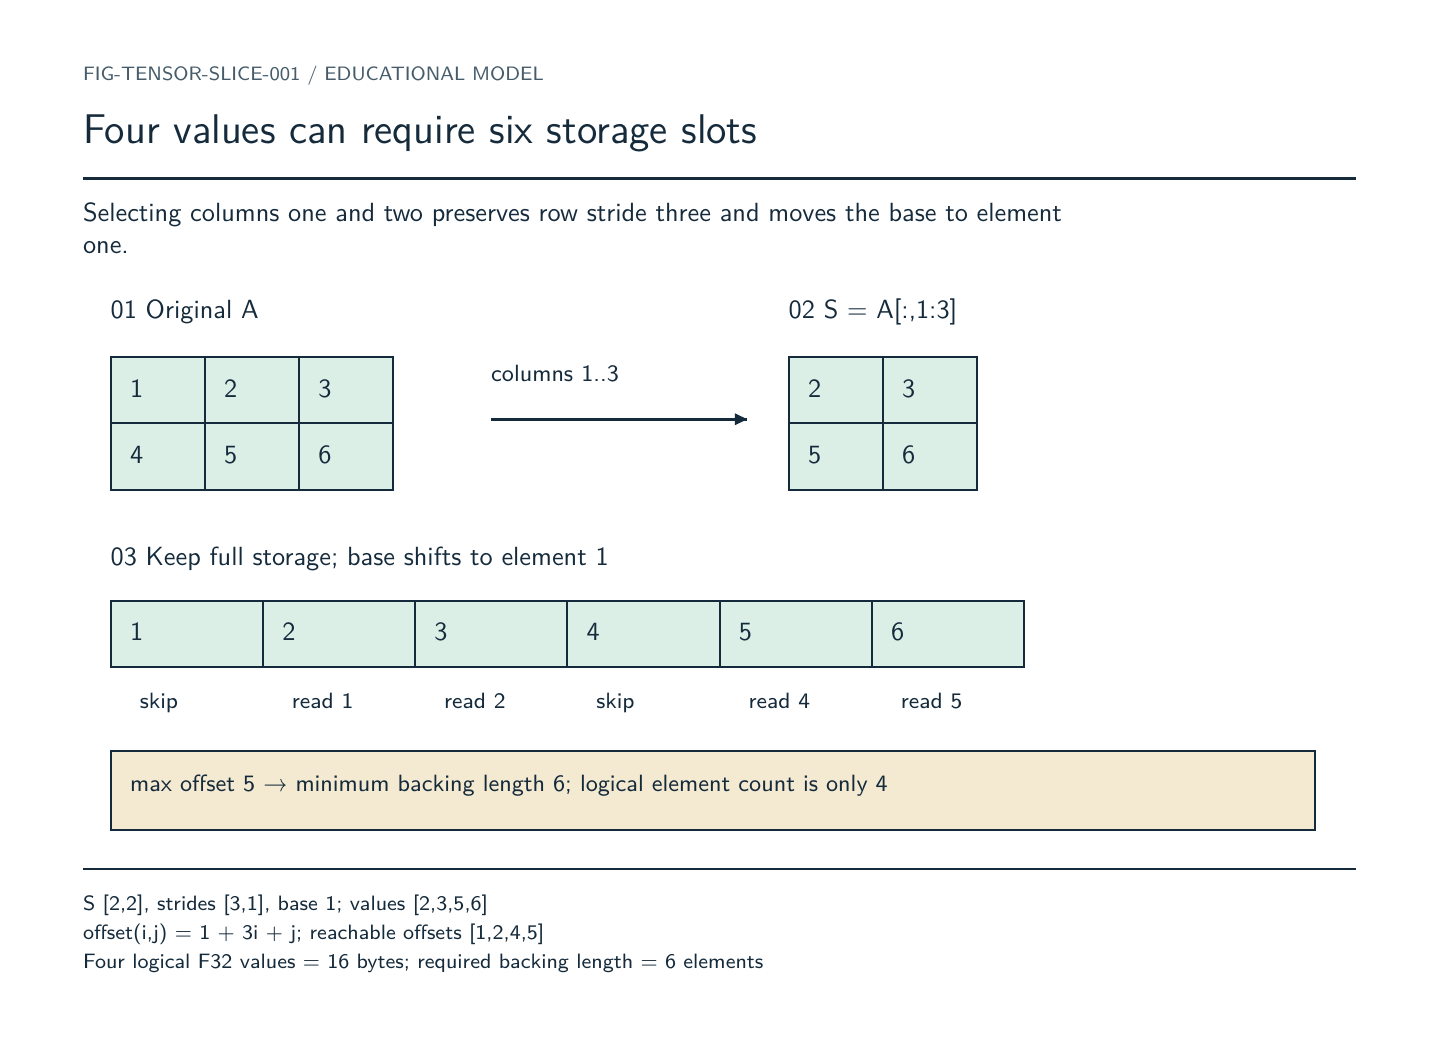
\begin{tikzpicture}[x=.5pt,y=-.5pt]
\path[use as bounding box] (0,0) rectangle (1000,720);
\path[fill=white,draw=none,line width=0.5pt] (0.0,0.0) rectangle (1000.0,720.0);
\node[inner sep=0pt,outer sep=0pt,anchor=base west,text={rgb,255:red,70;green,92;blue,107},font=\sffamily\fontsize{7.0}{8.4}\selectfont] at (40,38) {FIG-TENSOR-SLICE-001  /  EDUCATIONAL MODEL};
\node[inner sep=0pt,outer sep=0pt,anchor=base west,text={rgb,255:red,21;green,43;blue,60},font=\sffamily\fontsize{15.0}{18.0}\selectfont] at (40,84) {Four values can require six storage slots};
\draw[fill=none,draw={rgb,255:red,21;green,43;blue,60},line width=0.75pt] (40,109) -- (960,109);
\node[inner sep=0pt,outer sep=0pt,anchor=base west,text={rgb,255:red,21;green,43;blue,60},font=\sffamily\fontsize{9.5}{11.4}\selectfont] at (40,140) {Selecting columns one and two preserves row stride three and moves the base to element};
\node[inner sep=0pt,outer sep=0pt,anchor=base west,text={rgb,255:red,21;green,43;blue,60},font=\sffamily\fontsize{9.5}{11.4}\selectfont] at (40,163) {one.};
\node[inner sep=0pt,outer sep=0pt,anchor=base west,text={rgb,255:red,21;green,43;blue,60},font=\sffamily\fontsize{9.5}{11.4}\selectfont] at (60,210) {01  Original A};
\path[fill={rgb,255:red,220;green,239;blue,231},draw={rgb,255:red,21;green,43;blue,60},line width=0.7pt] (60.0,238.0) rectangle (128.0,286.0);
\node[inner sep=0pt,outer sep=0pt,anchor=base west,text={rgb,255:red,21;green,43;blue,60},font=\sffamily\fontsize{9.5}{11.4}\selectfont] at (74,267) {1};
\path[fill={rgb,255:red,220;green,239;blue,231},draw={rgb,255:red,21;green,43;blue,60},line width=0.7pt] (128.0,238.0) rectangle (196.0,286.0);
\node[inner sep=0pt,outer sep=0pt,anchor=base west,text={rgb,255:red,21;green,43;blue,60},font=\sffamily\fontsize{9.5}{11.4}\selectfont] at (142,267) {2};
\path[fill={rgb,255:red,220;green,239;blue,231},draw={rgb,255:red,21;green,43;blue,60},line width=0.7pt] (196.0,238.0) rectangle (264.0,286.0);
\node[inner sep=0pt,outer sep=0pt,anchor=base west,text={rgb,255:red,21;green,43;blue,60},font=\sffamily\fontsize{9.5}{11.4}\selectfont] at (210,267) {3};
\path[fill={rgb,255:red,220;green,239;blue,231},draw={rgb,255:red,21;green,43;blue,60},line width=0.7pt] (60.0,286.0) rectangle (128.0,334.0);
\node[inner sep=0pt,outer sep=0pt,anchor=base west,text={rgb,255:red,21;green,43;blue,60},font=\sffamily\fontsize{9.5}{11.4}\selectfont] at (74,315) {4};
\path[fill={rgb,255:red,220;green,239;blue,231},draw={rgb,255:red,21;green,43;blue,60},line width=0.7pt] (128.0,286.0) rectangle (196.0,334.0);
\node[inner sep=0pt,outer sep=0pt,anchor=base west,text={rgb,255:red,21;green,43;blue,60},font=\sffamily\fontsize{9.5}{11.4}\selectfont] at (142,315) {5};
\path[fill={rgb,255:red,220;green,239;blue,231},draw={rgb,255:red,21;green,43;blue,60},line width=0.7pt] (196.0,286.0) rectangle (264.0,334.0);
\node[inner sep=0pt,outer sep=0pt,anchor=base west,text={rgb,255:red,21;green,43;blue,60},font=\sffamily\fontsize{9.5}{11.4}\selectfont] at (210,315) {6};
\draw[fill=none,draw={rgb,255:red,21;green,43;blue,60},line width=1.25pt] (335,283) -- (520,283);
\path[fill={rgb,255:red,21;green,43;blue,60},draw=none,line width=0.5pt] (520.00,283.00) -- (511.00,287.35) -- (511.00,278.65) -- cycle;
\node[inner sep=0pt,outer sep=0pt,anchor=base west,text={rgb,255:red,21;green,43;blue,60},font=\sffamily\fontsize{8.5}{10.2}\selectfont] at (335,256) {columns 1..3};
\node[inner sep=0pt,outer sep=0pt,anchor=base west,text={rgb,255:red,21;green,43;blue,60},font=\sffamily\fontsize{9.5}{11.4}\selectfont] at (550,210) {02  S = A[:,1:3]};
\path[fill={rgb,255:red,220;green,239;blue,231},draw={rgb,255:red,21;green,43;blue,60},line width=0.7pt] (550.0,238.0) rectangle (618.0,286.0);
\node[inner sep=0pt,outer sep=0pt,anchor=base west,text={rgb,255:red,21;green,43;blue,60},font=\sffamily\fontsize{9.5}{11.4}\selectfont] at (564,267) {2};
\path[fill={rgb,255:red,220;green,239;blue,231},draw={rgb,255:red,21;green,43;blue,60},line width=0.7pt] (618.0,238.0) rectangle (686.0,286.0);
\node[inner sep=0pt,outer sep=0pt,anchor=base west,text={rgb,255:red,21;green,43;blue,60},font=\sffamily\fontsize{9.5}{11.4}\selectfont] at (632,267) {3};
\path[fill={rgb,255:red,220;green,239;blue,231},draw={rgb,255:red,21;green,43;blue,60},line width=0.7pt] (550.0,286.0) rectangle (618.0,334.0);
\node[inner sep=0pt,outer sep=0pt,anchor=base west,text={rgb,255:red,21;green,43;blue,60},font=\sffamily\fontsize{9.5}{11.4}\selectfont] at (564,315) {5};
\path[fill={rgb,255:red,220;green,239;blue,231},draw={rgb,255:red,21;green,43;blue,60},line width=0.7pt] (618.0,286.0) rectangle (686.0,334.0);
\node[inner sep=0pt,outer sep=0pt,anchor=base west,text={rgb,255:red,21;green,43;blue,60},font=\sffamily\fontsize{9.5}{11.4}\selectfont] at (632,315) {6};
\node[inner sep=0pt,outer sep=0pt,anchor=base west,text={rgb,255:red,21;green,43;blue,60},font=\sffamily\fontsize{9.5}{11.4}\selectfont] at (60,389) {03  Keep full storage; base shifts to element 1};
\path[fill={rgb,255:red,220;green,239;blue,231},draw={rgb,255:red,21;green,43;blue,60},line width=0.7pt] (60.0,414.0) rectangle (170.0,462.0);
\node[inner sep=0pt,outer sep=0pt,anchor=base west,text={rgb,255:red,21;green,43;blue,60},font=\sffamily\fontsize{9.5}{11.4}\selectfont] at (74,443) {1};
\path[fill={rgb,255:red,220;green,239;blue,231},draw={rgb,255:red,21;green,43;blue,60},line width=0.7pt] (170.0,414.0) rectangle (280.0,462.0);
\node[inner sep=0pt,outer sep=0pt,anchor=base west,text={rgb,255:red,21;green,43;blue,60},font=\sffamily\fontsize{9.5}{11.4}\selectfont] at (184,443) {2};
\path[fill={rgb,255:red,220;green,239;blue,231},draw={rgb,255:red,21;green,43;blue,60},line width=0.7pt] (280.0,414.0) rectangle (390.0,462.0);
\node[inner sep=0pt,outer sep=0pt,anchor=base west,text={rgb,255:red,21;green,43;blue,60},font=\sffamily\fontsize{9.5}{11.4}\selectfont] at (294,443) {3};
\path[fill={rgb,255:red,220;green,239;blue,231},draw={rgb,255:red,21;green,43;blue,60},line width=0.7pt] (390.0,414.0) rectangle (500.0,462.0);
\node[inner sep=0pt,outer sep=0pt,anchor=base west,text={rgb,255:red,21;green,43;blue,60},font=\sffamily\fontsize{9.5}{11.4}\selectfont] at (404,443) {4};
\path[fill={rgb,255:red,220;green,239;blue,231},draw={rgb,255:red,21;green,43;blue,60},line width=0.7pt] (500.0,414.0) rectangle (610.0,462.0);
\node[inner sep=0pt,outer sep=0pt,anchor=base west,text={rgb,255:red,21;green,43;blue,60},font=\sffamily\fontsize{9.5}{11.4}\selectfont] at (514,443) {5};
\path[fill={rgb,255:red,220;green,239;blue,231},draw={rgb,255:red,21;green,43;blue,60},line width=0.7pt] (610.0,414.0) rectangle (720.0,462.0);
\node[inner sep=0pt,outer sep=0pt,anchor=base west,text={rgb,255:red,21;green,43;blue,60},font=\sffamily\fontsize{9.5}{11.4}\selectfont] at (624,443) {6};
\node[inner sep=0pt,outer sep=0pt,anchor=base west,text={rgb,255:red,21;green,43;blue,60},font=\sffamily\fontsize{8.0}{9.6}\selectfont] at (81,492) {skip};
\node[inner sep=0pt,outer sep=0pt,anchor=base west,text={rgb,255:red,21;green,43;blue,60},font=\sffamily\fontsize{8.0}{9.6}\selectfont] at (191,492) {read 1};
\node[inner sep=0pt,outer sep=0pt,anchor=base west,text={rgb,255:red,21;green,43;blue,60},font=\sffamily\fontsize{8.0}{9.6}\selectfont] at (301,492) {read 2};
\node[inner sep=0pt,outer sep=0pt,anchor=base west,text={rgb,255:red,21;green,43;blue,60},font=\sffamily\fontsize{8.0}{9.6}\selectfont] at (411,492) {skip};
\node[inner sep=0pt,outer sep=0pt,anchor=base west,text={rgb,255:red,21;green,43;blue,60},font=\sffamily\fontsize{8.0}{9.6}\selectfont] at (521,492) {read 4};
\node[inner sep=0pt,outer sep=0pt,anchor=base west,text={rgb,255:red,21;green,43;blue,60},font=\sffamily\fontsize{8.0}{9.6}\selectfont] at (631,492) {read 5};
\path[fill={rgb,255:red,244;green,234;blue,210},draw={rgb,255:red,21;green,43;blue,60},line width=0.7pt] (60.0,523.0) rectangle (930.0,580.0);
\node[inner sep=0pt,outer sep=0pt,anchor=base west,text={rgb,255:red,21;green,43;blue,60},font=\sffamily\fontsize{8.5}{10.2}\selectfont] at (74,552) {max offset 5 → minimum backing length 6; logical element count is only 4};
\draw[fill=none,draw={rgb,255:red,21;green,43;blue,60},line width=0.75pt] (40,608) -- (960,608);
\node[inner sep=0pt,outer sep=0pt,anchor=base west,text={rgb,255:red,21;green,43;blue,60},font=\sffamily\fontsize{7.5}{9.0}\selectfont] at (40,638) {S [2,2], strides [3,1], base 1; values [2,3,5,6]};
\node[inner sep=0pt,outer sep=0pt,anchor=base west,text={rgb,255:red,21;green,43;blue,60},font=\sffamily\fontsize{7.5}{9.0}\selectfont] at (40,659) {offset(i,j) = 1 + 3i + j; reachable offsets [1,2,4,5]};
\node[inner sep=0pt,outer sep=0pt,anchor=base west,text={rgb,255:red,21;green,43;blue,60},font=\sffamily\fontsize{7.5}{9.0}\selectfont] at (40,680) {Four logical F32 values = 16 bytes; required backing length = 6 elements};
\end{tikzpicture}
}\caption{A column slice retains gaps in storage and needs a larger backing range than its logical element count.}\end{figure}

Return to the six-value matrix and select columns \texttt{1..3} using
\texttt{\seqsplit{slice\_axis(1,1,3)}}. The result is
\texttt{{[}{[}2,3{]},{[}5,6{]}{]}}. Its shape is \texttt{{[}2,2{]}}, its
strides remain \texttt{{[}3,1{]}}, and its base is 1. The offset formula
becomes

\[
o_S(i,j)=1+3i+j,\qquad 0\le i<2,\quad 0\le j<2.
\]

The four coordinates reach offsets \texttt{{[}1,2,4,5{]}}. The logical
payload is four F32 values, or 16 bytes, but a borrowed storage slice
addressed from its own index zero must have length at least 6. It must
include the preceding element and the gap, even though those elements
are never logically read by this view. This is why ``four values'' and
``six backing slots'' are compatible facts. The test passes a
five-element backing slice with the same metadata and requires
\texttt{\seqsplit{InvalidViewExtent}} before any value can be read.

\subsection{Mutable aliasing is a numerical
hazard}\label{mutable-aliasing-is-a-numerical-hazard}

Two overlapping immutable views are safe. Two overlapping writable views
can race or make one operation observe another's partial output. The
result may be nondeterministic without ever becoming NaN or crashing.
Ownership is therefore a numerical correctness concern.

V1 does not offer a constructor for arbitrary mutable strides. An owner
can produce one \texttt{TensorViewMut} over its complete canonical
storage. That operation borrows the owner exclusively. While the mutable
view is live, Rust prevents another shared or mutable view from
coexisting.

\begin{verbatim}
let mut tensor = OwnedTensor::zeros(vec![2, 3])?;
{
    let mut writable = tensor.view_mut();
    *writable.get_mut(&[1, 2])? = 7.0;
}
assert_eq!(*tensor.view().get(&[1, 2])?, 7.0);
\end{verbatim}

\begin{figure}[H]\centering\resizebox{\linewidth}{!}{% Generated from figures/generated/tensor-lifetime.svg; do not hand edit.
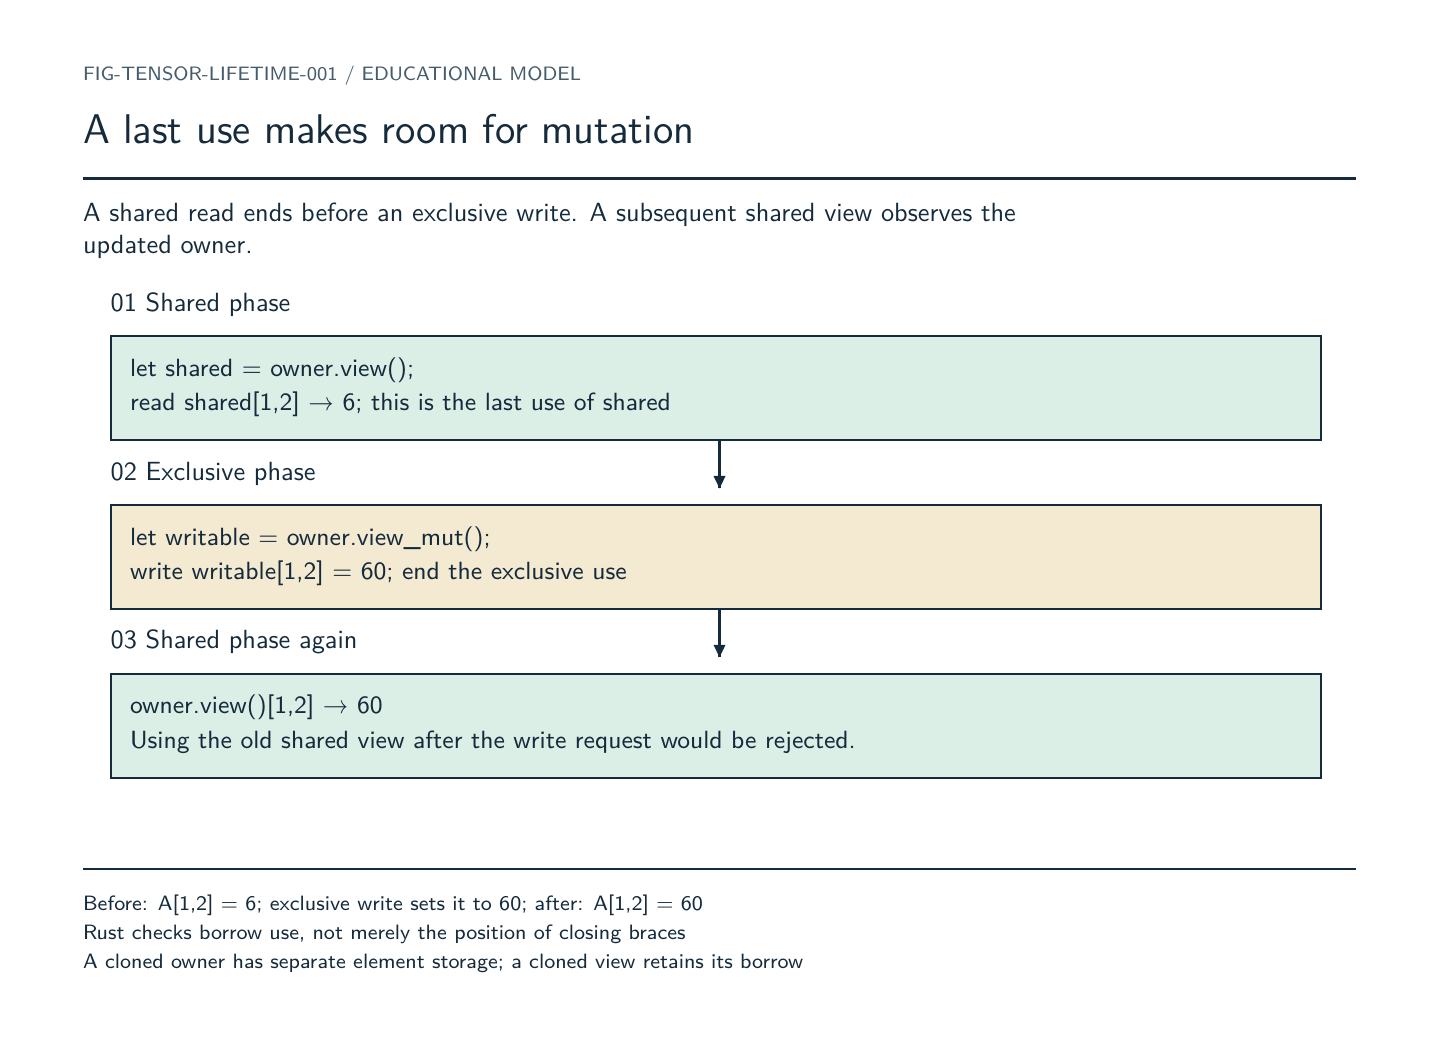
\begin{tikzpicture}[x=.5pt,y=-.5pt]
\path[use as bounding box] (0,0) rectangle (1000,720);
\path[fill=white,draw=none,line width=0.5pt] (0.0,0.0) rectangle (1000.0,720.0);
\node[inner sep=0pt,outer sep=0pt,anchor=base west,text={rgb,255:red,70;green,92;blue,107},font=\sffamily\fontsize{7.0}{8.4}\selectfont] at (40,38) {FIG-TENSOR-LIFETIME-001  /  EDUCATIONAL MODEL};
\node[inner sep=0pt,outer sep=0pt,anchor=base west,text={rgb,255:red,21;green,43;blue,60},font=\sffamily\fontsize{15.0}{18.0}\selectfont] at (40,84) {A last use makes room for mutation};
\draw[fill=none,draw={rgb,255:red,21;green,43;blue,60},line width=0.75pt] (40,109) -- (960,109);
\node[inner sep=0pt,outer sep=0pt,anchor=base west,text={rgb,255:red,21;green,43;blue,60},font=\sffamily\fontsize{9.5}{11.4}\selectfont] at (40,140) {A shared read ends before an exclusive write. A subsequent shared view observes the};
\node[inner sep=0pt,outer sep=0pt,anchor=base west,text={rgb,255:red,21;green,43;blue,60},font=\sffamily\fontsize{9.5}{11.4}\selectfont] at (40,163) {updated owner.};
\node[inner sep=0pt,outer sep=0pt,anchor=base west,text={rgb,255:red,21;green,43;blue,60},font=\sffamily\fontsize{9.5}{11.4}\selectfont] at (60,205) {01  Shared phase};
\path[fill={rgb,255:red,220;green,239;blue,231},draw={rgb,255:red,21;green,43;blue,60},line width=0.7pt] (60.0,223.0) rectangle (935.0,298.0);
\node[inner sep=0pt,outer sep=0pt,anchor=base west,text={rgb,255:red,21;green,43;blue,60},font=\sffamily\fontsize{9.0}{10.799999999999999}\selectfont] at (74,252) {let shared = owner.view();};
\node[inner sep=0pt,outer sep=0pt,anchor=base west,text={rgb,255:red,21;green,43;blue,60},font=\sffamily\fontsize{9.0}{10.799999999999999}\selectfont] at (74,277) {read shared[1,2] → 6; this is the last use of shared};
\node[inner sep=0pt,outer sep=0pt,anchor=base west,text={rgb,255:red,21;green,43;blue,60},font=\sffamily\fontsize{9.5}{11.4}\selectfont] at (60,327) {02  Exclusive phase};
\path[fill={rgb,255:red,244;green,234;blue,210},draw={rgb,255:red,21;green,43;blue,60},line width=0.7pt] (60.0,345.0) rectangle (935.0,420.0);
\node[inner sep=0pt,outer sep=0pt,anchor=base west,text={rgb,255:red,21;green,43;blue,60},font=\sffamily\fontsize{9.0}{10.799999999999999}\selectfont] at (74,374) {let writable = owner.view\_mut();};
\node[inner sep=0pt,outer sep=0pt,anchor=base west,text={rgb,255:red,21;green,43;blue,60},font=\sffamily\fontsize{9.0}{10.799999999999999}\selectfont] at (74,399) {write writable[1,2] = 60; end the exclusive use};
\node[inner sep=0pt,outer sep=0pt,anchor=base west,text={rgb,255:red,21;green,43;blue,60},font=\sffamily\fontsize{9.5}{11.4}\selectfont] at (60,449) {03  Shared phase again};
\path[fill={rgb,255:red,220;green,239;blue,231},draw={rgb,255:red,21;green,43;blue,60},line width=0.7pt] (60.0,467.0) rectangle (935.0,542.0);
\node[inner sep=0pt,outer sep=0pt,anchor=base west,text={rgb,255:red,21;green,43;blue,60},font=\sffamily\fontsize{9.0}{10.799999999999999}\selectfont] at (74,496) {owner.view()[1,2] → 60};
\node[inner sep=0pt,outer sep=0pt,anchor=base west,text={rgb,255:red,21;green,43;blue,60},font=\sffamily\fontsize{9.0}{10.799999999999999}\selectfont] at (74,521) {Using the old shared view after the write request would be rejected.};
\draw[fill=none,draw={rgb,255:red,21;green,43;blue,60},line width=1.25pt] (500,298) -- (500,333);
\path[fill={rgb,255:red,21;green,43;blue,60},draw=none,line width=0.5pt] (500.00,333.00) -- (495.65,324.00) -- (504.35,324.00) -- cycle;
\draw[fill=none,draw={rgb,255:red,21;green,43;blue,60},line width=1.25pt] (500,420) -- (500,455);
\path[fill={rgb,255:red,21;green,43;blue,60},draw=none,line width=0.5pt] (500.00,455.00) -- (495.65,446.00) -- (504.35,446.00) -- cycle;
\draw[fill=none,draw={rgb,255:red,21;green,43;blue,60},line width=0.75pt] (40,608) -- (960,608);
\node[inner sep=0pt,outer sep=0pt,anchor=base west,text={rgb,255:red,21;green,43;blue,60},font=\sffamily\fontsize{7.5}{9.0}\selectfont] at (40,638) {Before: A[1,2] = 6; exclusive write sets it to 60; after: A[1,2] = 60};
\node[inner sep=0pt,outer sep=0pt,anchor=base west,text={rgb,255:red,21;green,43;blue,60},font=\sffamily\fontsize{7.5}{9.0}\selectfont] at (40,659) {Rust checks borrow use, not merely the position of closing braces};
\node[inner sep=0pt,outer sep=0pt,anchor=base west,text={rgb,255:red,21;green,43;blue,60},font=\sffamily\fontsize{7.5}{9.0}\selectfont] at (40,680) {A cloned owner has separate element storage; a cloned view retains its borrow};
\end{tikzpicture}
}\caption{Shared reads end before exclusive mutation, and a later shared view observes the new value.}\end{figure}

In the recurring fixture, a shared read sees 6, its last use ends, an
exclusive view writes 60, and a later shared view sees 60. The
successful transition is covered by a normal Rust test. Two
\texttt{compile\_fail} documentation tests verify the forbidden cases:
using a shared view after requesting overlapping mutable access, and
returning a view of a local owner. These failures are checked by the
compiler as part of \texttt{cargo\ test\ -\/-doc}; no intentionally
broken file is placed in a normal test target.
\href{https://github.com/hermonai/inside-the-llm-engine/blob/astra-visual-rewrite/figures/generated/tensor-lifetime.txt}{Text
lifetime trace}.

A future safe split operation could prove that two canonical ranges do
not overlap before returning two mutable borrows. Chapter 5 does not
need it. It also needs no unsafe code: \texttt{engine0} retains
\texttt{\seqsplit{\#![forbid(unsafe\_code)]}}.

\subsection{Physical addresses, alignment, and
locality}\label{physical-addresses-alignment-and-locality}

\texttt{Vec\textless{}f32\textgreater{}} stores initialized \texttt{f32}
elements contiguously. If an illustrative base address were
\texttt{0x1000}, consecutive elements would begin at \texttt{0x1000},
\texttt{0x1004}, \texttt{0x1008}, and so on. Real allocator addresses
vary; the point is the four-byte displacement, not those invented
addresses.

The allocation is aligned suitably for \texttt{f32}. That does not
promise alignment for a future SIMD instruction, GPU buffer, stable C
ABI, or direct I/O request. Part VII will make arena and native
alignment explicit.

Layout also affects locality. CPU caches fetch regions larger than one
scalar, so visiting neighboring physical elements often benefits from
already-fetched data. For a row-major \texttt{{[}N,N{]}} matrix,
row-then-column iteration visits offsets \texttt{0,1,2,...}.
Column-then-row iteration visits \texttt{0,N,2N,...}, then
\texttt{1,N+1,2N+1,...}. The mathematical checksum can be identical
while the memory access pattern differs.

This is a preview, not a cache-architecture chapter. Associativity,
cache levels, hardware prefetching, NUMA, and kernel tiling remain
ahead.

\subsection{Build Tensor Substrate v1}\label{build-tensor-substrate-v1}

The implementation lives in \texttt{engine0::tensor}. A module is
enough: a separate crate would add a dependency boundary before another
consumer exists.

\begin{verbatim}
pub struct OwnedTensor {
    shape: Vec<usize>,
    strides: Vec<usize>,
    data: Vec<f32>,
}
\end{verbatim}

The owner stores canonical strides although they are derivable.
Constructors validate that redundancy once; repeated indexing and debug
output can then use the complete layout without recomputing metadata.
Dynamic rank was chosen over const generics because later operations
naturally move among vectors, matrices, and higher-rank activations. Our
purpose is to inspect runtime tensor metadata, not encode every rank
into a different Rust type.

The v1 public surface fits on one conceptual page:

\begin{itemize}
\tightlist
\item
  construct with \texttt{from\_vec} or \texttt{zeros};
\item
  inspect dtype, rank, shape, strides, length, and physical slice;
\item
  create canonical immutable or exclusive mutable views;
\item
  create a validated general immutable view from parts;
\item
  read through \texttt{get} or \texttt{get2};
\item
  create rank-2 transpose, bounded slice, or canonical reshape views;
\item
  explicitly materialize with \texttt{to\_contiguous};
\item
  call checked count, byte-count, stride, and offset helpers.
\end{itemize}

There is no broadcasting, autograd, device method, negative stride,
fancy indexing, generic operator graph, quantized dtype, BLAS dispatch,
SIMD, or GPU path. A tensor describes data. It does not own execution.

\subsection{Migrate ENGINE-1 without changing
it}\label{migrate-engine-1-without-changing-it}

Before this chapter, \texttt{\seqsplit{TinyLanguageModel}} stored
embedding and projection as bare vectors and indexed both manually. They
are now immutable \texttt{OwnedTensor} values with shape
\texttt{{[}V,D{]}} and strides \texttt{{[}D,1{]}}. The scalar forward
loop remains visible:

\[
z_i=b_i+\sum_{j=0}^{D-1}W_{i,j}h_j,
\qquad
\mathbf{W}\in\mathbb{R}^{V_{\mathrm{vocab}}\times D},
\quad \mathbf{h}\in\mathbb{R}^{D},
\quad \mathbf{z}\in\mathbb{R}^{V_{\mathrm{vocab}}}.
\]

The model owns \(W\) with shape \texttt{{[}V,D{]}}, the request owns
\(h\) with shape \texttt{{[}D{]}}, and the forward result owns logits
\(z\) with shape \texttt{{[}V{]}}. Storage and accumulation are
\texttt{f32} in this tiny implementation. Each \texttt{W{[}i,j{]}} and
embedding element is now reached through checked \texttt{get2}; no
matrix multiplication operator has been smuggled into \texttt{Tensor}.

Bias, hidden activation, and \texttt{Logits} remain specialized
one-dimensional vectors. Wrapping every vector would increase
abstraction without eliminating an ambiguous multi-axis indexing
assumption. Chapter 6 can revisit activation representations when
operators need common tensor inputs.

This refactor is our first internal substitution gate. The
representation changed; model semantics did not. The full hand oracle
still gives \texttt{\seqsplit{[-0.7,0.1,0.4,2.2]}} for token
\texttt{like}, and greedy generation still emits \texttt{Rust} followed
by EOS.

\subsection{Prove the memory model
independently}\label{prove-the-memory-model-independently}

The plain-Python oracle does not import Rust code. It derives
\texttt{{[}12,4,1{]}} for shape \texttt{{[}2,3,4{]}}, maps
\texttt{{[}1,2,3{]}} to 23, enumerates the \texttt{{[}2,3{]}} matrix at
physical offsets \texttt{{[}0,1,2,3,4,5{]}}, and proves two different
\texttt{{[}3,2{]}} interpretations:

\begin{itemize}
\tightlist
\item
  reshape offsets: \texttt{{[}0,1,2,3,4,5{]}};
\item
  transpose offsets: \texttt{{[}0,3,1,4,2,5{]}}.
\end{itemize}

The transposed logical copy is exactly \texttt{{[}A,D,B,E,C,F{]}}. These
are integer and symbolic results, so no floating-point tolerance is
needed.

Run it from the repository root:

\begin{verbatim}
python3 code/reference/python/chapter05_tensor_oracle.py
\end{verbatim}

The Rust suite adds deterministic generated shapes of ranks one through
four. Every canonical logical index must map to its flat row-major
index, and the largest index must map to \texttt{element\_count\ -\ 1}.
Boundary tests exercise shape, byte, stride, offset, and extent overflow
without attempting giant allocations.

\subsection{Performance lab: same sum, different
walk}\label{performance-lab-same-sum-different-walk}

The Chapter 5 harness allocates one canonical \texttt{{[}2048,2048{]}}
tensor---4,194,304 \texttt{f32} values, or 16 MiB---and accumulates
every value as \texttt{f64}. It alternates row-major and column-wise
traversal across seven warmed release repetitions. Both orders produce
the exact checksum \texttt{524280621.0}.

On the recorded Apple M1 system, medians were:

{\def\LTcaptype{none} % do not increment counter
\begin{longtable}[]{@{}lr@{}}
\toprule\noalign{}
Order & Median \\
\midrule\noalign{}
\endhead
\bottomrule\noalign{}
\endlastfoot
Physical row-major & 4,163,875 ns \\
Column-wise logical & 13,692,583 ns \\
\end{longtable}
}

The durable
\href{https://github.com/hermonai/inside-the-llm-engine/blob/astra-visual-rewrite/research/benchmarks/chapter-05-traversal-order.md}{benchmark
record} contains the commit, command, hardware, software, shape,
repetitions, checksum, and raw result. It supports one narrow
observation: on that run, different access order had different cost. It
does not establish a universal ratio, isolate a cache level, or measure
matrix multiplication or inference.

\subsection{Follow the element, byte, and
owner}\label{follow-the-element-byte-and-owner}

One logical element now has a complete route:

\begin{center}\begin{adjustbox}{max width=\linewidth}% Legacy topology preserved as native vectors and typeset labels.
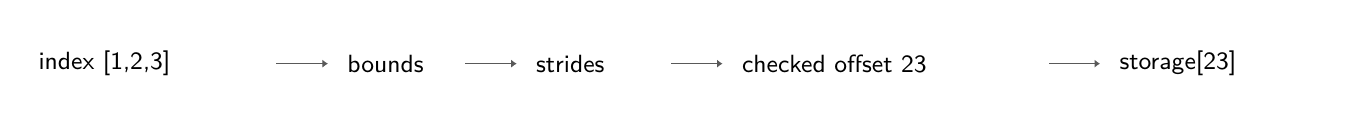
\begin{tikzpicture}[x=6.2pt,y=-13pt,draw=black!65,line width=.45pt]
\path[use as bounding box] (-1,-1) rectangle (75,1);
\draw (14,0) -- (13.5,0);
\draw (14,0) -- (14.5,0);
\draw (15,0) -- (14.5,0);
\draw (15,0) -- (15.5,0);
\draw[-{Latex[length=2pt,width=3pt]}] (15.5,0) -- (16.5,0);
\draw (25,0) -- (24.5,0);
\draw (25,0) -- (25.5,0);
\draw (26,0) -- (25.5,0);
\draw (26,0) -- (26.5,0);
\draw[-{Latex[length=2pt,width=3pt]}] (26.5,0) -- (27.5,0);
\draw (37,0) -- (36.5,0);
\draw (37,0) -- (37.5,0);
\draw (38,0) -- (37.5,0);
\draw (38,0) -- (38.5,0);
\draw[-{Latex[length=2pt,width=3pt]}] (38.5,0) -- (39.5,0);
\draw (59,0) -- (58.5,0);
\draw (59,0) -- (59.5,0);
\draw (60,0) -- (59.5,0);
\draw (60,0) -- (60.5,0);
\draw[-{Latex[length=2pt,width=3pt]}] (60.5,0) -- (61.5,0);
\node[anchor=west,inner sep=0pt,font=\sffamily\fontsize{9}{11}\selectfont] at (-0.4,0) {\begin{adjustbox}{max width=80.60000000000001pt}index [1,2,3]\end{adjustbox}};
\node[anchor=west,inner sep=0pt,font=\sffamily\fontsize{9}{11}\selectfont] at (17.6,0) {\begin{adjustbox}{max width=37.2pt}bounds\end{adjustbox}};
\node[anchor=west,inner sep=0pt,font=\sffamily\fontsize{9}{11}\selectfont] at (28.6,0) {\begin{adjustbox}{max width=43.4pt}strides\end{adjustbox}};
\node[anchor=west,inner sep=0pt,font=\sffamily\fontsize{9}{11}\selectfont] at (40.6,0) {\begin{adjustbox}{max width=105.4pt}checked offset 23\end{adjustbox}};
\node[anchor=west,inner sep=0pt,font=\sffamily\fontsize{9}{11}\selectfont] at (62.6,0) {\begin{adjustbox}{max width=68.2pt}storage[23]\end{adjustbox}};
\end{tikzpicture}
\end{adjustbox}\end{center}

See
\href{https://github.com/hermonai/inside-the-llm-engine/blob/astra-visual-rewrite/diagrams/tensor/follow-the-element.txt}{Follow
the Element}. The route is where mathematical coordinates meet
memory-safe code.

The byte journey begins at an owned
\texttt{Vec\textless{}f32\textgreater{}}. Views, slices, reshapes, and
transposes change metadata while borrowing the same payload. Only
\texttt{to\_contiguous} creates a new allocation and moves logical
values into canonical order.
\href{https://github.com/hermonai/inside-the-llm-engine/blob/astra-visual-rewrite/diagrams/tensor/follow-the-byte.txt}{Follow
the Byte} records that fork.

The ownership journey begins with \texttt{OwnedTensor}, fans out into
immutable borrowed interpretations, and either ends those views before
the owner or creates an explicit independent copy.
\href{https://github.com/hermonai/inside-the-llm-engine/blob/astra-visual-rewrite/diagrams/tensor/follow-the-owner.txt}{Follow
the Owner} shows the lifetime boundary.

\subsection{A complete worked view}\label{a-complete-worked-view}

Let us run one allocation through every v1 metadata operation. Begin
with twelve values in canonical shape \texttt{{[}4,3{]}}:

\[
X=
\begin{bmatrix}
0&1&2\\
3&4&5\\
6&7&8\\
9&10&11
\end{bmatrix}.
\]

\texttt{OwnedTensor::from\_vec({[}4,3{]},\ data)} calculates 12
elements, checks the data length, derives strides \texttt{{[}3,1{]}},
and takes ownership of the caller's vector. The separate
\texttt{\seqsplit{checked\_byte\_count}} helper establishes the 48-byte
payload; \texttt{from\_vec} does not call that helper. Its input is
already an initialized Rust vector, not an unchecked external byte
range. The logical coordinate \texttt{{[}2,1{]}} passes bounds \(2<4\)
and \(1<3\), then maps to

\[
0 + 2\times3 + 1\times1 = 7.
\]

Storage element 7 contains value 7. No pointer arithmetic is exposed to
the caller.

Now take rows \texttt{1..3}. The slice has shape \texttt{{[}2,3{]}},
preserves strides \texttt{{[}3,1{]}}, and moves the base to

\[
b'=0+1\times3=3.
\]

Its logical \texttt{{[}0,0{]}} reaches owner offset 3;
\texttt{{[}1,2{]}} reaches \(3+1\times3+2\times1=8\). The largest
reachable offset is 8, so a storage length of at least 9 is sufficient
for this view even though its owner contains 12 values. The view remains
canonical under v1's stride definition: shape \texttt{{[}2,3{]}} expects
\texttt{{[}3,1{]}}. It occupies one dense subregion from offsets 3
through 8.

Transpose that slice. Shape becomes \texttt{{[}3,2{]}}, strides become
\texttt{{[}1,3{]}}, and base remains 3. Logical \texttt{{[}2,1{]}} still
reaches offset

\[
3+2\times1+1\times3=8,
\]

but logical iteration visits offsets \texttt{{[}3,6,4,7,5,8{]}}. This is
valid and non-contiguous. \texttt{\seqsplit{reshape\_view([6])}} refuses
it because v1 cannot reinterpret that logical walk as canonical physical
order without moving values.

Finally, \texttt{to\_contiguous} enumerates those six logical
coordinates, reads \texttt{{[}3,6,4,7,5,8{]}}, and creates a new
\texttt{{[}3,2{]}} owner whose physical storage holds exactly that
sequence with strides \texttt{{[}2,1{]}}. Source and destination have
equal logical values but different ownership and physical order.
Mutating the new owner cannot affect \(X\).

This worked path separates four statements that are easy to collapse:

\begin{itemize}
\tightlist
\item
  the original owner is contiguous;
\item
  the row slice is also contiguous but begins at a nonzero base;
\item
  the transpose is a valid non-contiguous alias;
\item
  the materialized result is a separate contiguous owner.
\end{itemize}

No single \texttt{shape} or \texttt{element\_count} field can prove all
four.

\subsection{Error taxonomy is part of the
API}\label{error-taxonomy-is-part-of-the-api}

A checked tensor API needs errors precise enough to identify which
invariant failed. V1 keeps the list small while preserving that
distinction.

{\def\LTcaptype{none} % do not increment counter
\begin{longtable}[]{@{}
  >{\raggedright\arraybackslash}p{(\linewidth - 4\tabcolsep) * \real{0.3333}}
  >{\raggedright\arraybackslash}p{(\linewidth - 4\tabcolsep) * \real{0.3333}}
  >{\raggedright\arraybackslash}p{(\linewidth - 4\tabcolsep) * \real{0.3333}}@{}}
\toprule\noalign{}
\begin{minipage}[b]{\linewidth}\raggedright
Error
\end{minipage} & \begin{minipage}[b]{\linewidth}\raggedright
Rejected condition
\end{minipage} & \begin{minipage}[b]{\linewidth}\raggedright
Why it is separate
\end{minipage} \\
\midrule\noalign{}
\endhead
\bottomrule\noalign{}
\endlastfoot
\texttt{ShapeOverflow} & element or canonical-stride product does not
fit & prevents undersized or unrepresentable owners \\
\texttt{\seqsplit{ByteCountOverflow}} & elements times dtype width does
not fit & element count can fit while bytes do not \\
\texttt{\seqsplit{StorageLengthMismatch}} & owner shape and supplied
vector length disagree & owner construction requires exact storage \\
\texttt{\seqsplit{ShapeStrideRankMismatch}} & view metadata vectors have
different lengths & no axis-to-stride mapping exists \\
\texttt{RankMismatch} & an index has too few or too many axes & logical
coordinate is malformed \\
\texttt{\seqsplit{IndexOutOfBounds}} & one coordinate is outside its
dimension & logical bounds failed before addressing \\
\texttt{OffsetOverflow} & extent or index arithmetic cannot be
represented & prevents wrapped physical addresses \\
\texttt{\seqsplit{InvalidViewExtent}} & reachable offsets exceed
borrowed storage & arbitrary strides need more than count validation \\
\texttt{NonContiguous} & reshape source lacks canonical strides &
no-copy contract cannot be met \\
\texttt{\seqsplit{ReshapeElementMismatch}} & requested count changes &
reshape cannot create or discard values \\
\texttt{ExpectedMatrix} & transpose source is not rank 2 & v1 implements
only the promised operation \\
\texttt{InvalidSlice} & axis or half-open range is malformed & slicing
stays bounded and explicit \\
\end{longtable}
}

The display text helps a human; callers can match the typed variant. No
checked operation converts a malformed request into a default tensor or
clamps an index. Silent recovery would turn structural corruption into
plausible numbers.

There are still internal invariants. An \texttt{OwnedTensor} has already
proven that its strides are canonical and its storage count is exact.
Methods may rely on that fact, but public inputs pass through checked
construction. This boundary lets code remain readable without repeating
an entire model-file parser's threat model at every loop iteration.

\subsection{Why the type system stops
here}\label{why-the-type-system-stops-here}

It is tempting to encode every fact in Rust types:

\begin{verbatim}
Tensor<Element, Device, Layout, Rank, Shape, Allocator, Mutability, ...>
\end{verbatim}

Such a design can be valuable in a specialized library. It would be
harmful at this point in the book. Transformer intermediates change rank
and shape at runtime. Model metadata eventually arrives from files. If
the reader spends the chapter decoding const-generic machinery, the
physical memory model has again disappeared behind an abstraction.

Dynamic \texttt{Vec\textless{}usize\textgreater{}} metadata makes each
runtime check visible. \texttt{F32} makes one dtype concrete. An
immutable general view demonstrates real striding. A narrow mutable view
demonstrates exclusivity. This is enough structure to prevent the
current errors and enough simplicity to audit on one page.

The substrate is also intentionally not an operator object. Adding
methods such as \texttt{\seqsplit{tensor.matmul(other)}} would couple
data representation to arithmetic, temporary allocation, provider
choice, and error policy before those contracts have been derived.
Chapter 6 will accept tensor views as inputs to separately named
kernels. Later a planner may choose a scalar CPU, SIMD, Metal, or CUDA
implementation while the input tensor remains data plus metadata.

\subsection{Correctness matrix}\label{correctness-matrix}

The test suite does more than exercise happy-path indexing. Each group
protects a later inference-engine boundary.

\textbf{Construction tests} cover rank 0 through rank 4, exact shape
retrieval, canonical strides, dtype width, storage mismatch, zero
dimensions, element overflow, byte overflow, and canonical-stride
overflow. The overflow cases call helpers directly near
\texttt{usize::MAX}; they never attempt dangerous allocations.

\textbf{Indexing tests} cover first, middle, and final elements, the
hand-computed \texttt{{[}1,2,3{]}\ →\ 23} case, wrong-rank coordinates,
per-axis bounds, base offsets, extent overflow, and strides that require
more storage than logical count. A generated loop enumerates every
coordinate for small ranks one through four and requires the canonical
physical offset sequence exactly.

\textbf{View tests} prove rank-2 transpose shape, strides, and values;
compatible reshape shapes; rejection of incompatible and non-contiguous
reshape; bounded axis slicing; zero-length slices; zero-stride immutable
aliasing; and explicit logical-order materialization. Reference identity
proves a view reaches the owner's element rather than a copied value.

\textbf{Ownership tests} mutate one complete canonical owner through
\texttt{TensorViewMut}, end the exclusive borrow, and read the new value
through a later immutable view. A separately materialized owner is
mutated and the source is proven unchanged. Compile-time borrow failures
belong in Lab 21 rather than normal test sources, because committed test
targets must compile.

\textbf{Regression tests} retain every Part I contract: tokenizer
boundaries, strict UTF-8 streaming, full numerical logits, sampling
distributions, seeded state, token feedback, cancellation, EOS, budgets,
failure paths, and exactly one terminal outcome. The tensor refactor is
invalid if any of those observable semantics changes.

Together these are stronger evidence than testing one printed matrix.
Shape, layout, storage, and lifetime are orthogonal enough that each
deserves its own failure injection.

\subsection{Review from four engineering
perspectives}\label{review-from-four-engineering-perspectives}

A systems programmer should now be able to locate every allocation and
copy. The model owns parameter vectors. Views borrow them. Metadata
transforms do not move elements. \texttt{to\_contiguous} does. Size,
extent, and offset arithmetic are checked at public boundaries.

An ML engineer should recognize standard rank, shape, stride, transpose,
and view concepts while seeing the declared differences from NumPy and
PyTorch. Model equations retain their shapes. No layout detail changes
the mathematical meaning of \(z=Wh+b\).

A Rust engineer should find no dangling reference escape and no safe
path to arbitrary overlapping mutable strided views. Shared borrows can
coexist; exclusive mutation cannot overlap them. There is no
\texttt{unsafe}, and malformed public indexing returns typed errors.

A beginner should be able to answer the concrete question ``where is
\texttt{{[}1,2{]}}?'': check two bounds, multiply each coordinate by its
element stride, add the base, then read that physical element. The term
\emph{tensor} now expands into inspectable data instead of shrinking
into framework vocabulary.

\subsection{Inside Hermon}\label{inside-hermon-1}

The following findings were re-verified on 2026-09-06 at Hermon commit
\texttt{5e908d7} and its llama.cpp submodule \texttt{389ff61d}; they are
not claims about an uninspected future revision.

\begin{quote}
\textbf{INSIDE HERMON --- LIBRARY CONTRACT} \texttt{hermon-llamacpp}
contains one of the project's unsafe FFI boundaries;
\texttt{hermon-kernels} also contains native FFI code. The bridge's safe
\texttt{\seqsplit{Model::tensor\_info}} copies a tensor's GGML
dimensions, rank, and type across the FFI boundary.
\texttt{tensor\_row\_f32} borrows the model handle for the call and
returns one newly owned decoded row. The shim validates tensor
existence, shape, host residency, layout, conversion support, and caller
output length.
\end{quote}

The loaded model owns packed tensor lifetime; Rust callers do not
receive a raw borrow that can outlive it. Unsafe handle access is
localized and each wrapper block states its invariant.
\texttt{TensorSession} similarly owns reusable mutable GGML scratch
state, is movable between threads, but is deliberately not
\texttt{Sync}; entry points require exclusive \texttt{\&mut} access.

\begin{quote}
\textbf{INSIDE HERMON --- LIBRARY} \texttt{hermon-gguf} exposes names,
dimensions, per-tensor serialized type, offsets, and checked byte
lengths. It can open an exactly bounded reader or read a checked
subrange without materializing the whole tensor. That proves parser
behavior, not that the default inference path uses Hermon-native
tensors.
\end{quote}

\begin{quote}
\textbf{INSIDE HERMON --- PREVIEW} The gated paged GGUF runtime combines
validated metadata with the llama.cpp packed tensor bridge. It keeps a
\texttt{TensorSession} behind a mutex for exclusive graph/scratch use.
The default production batched path remains llama.cpp managed, so
PREVIEW tensor plumbing must not be flattened into a CURRENT end-to-end
claim.
\end{quote}

Pinned GGML reinforces the same lesson. Its \texttt{ggml\_tensor}
records type, dimensions \texttt{ne}, byte strides \texttt{nb},
storage/buffer information, and view/source metadata because operations
cannot assume contiguity. GGML fixes a maximum rank and has packed dtype
concerns that v1 excludes. The shared principle is not API identity:
kernels need shape, layout, type, and lifetime facts together.

\begin{figure}[H]\centering\resizebox{\linewidth}{!}{% Generated from figures/generated/tensor-production.svg; do not hand edit.
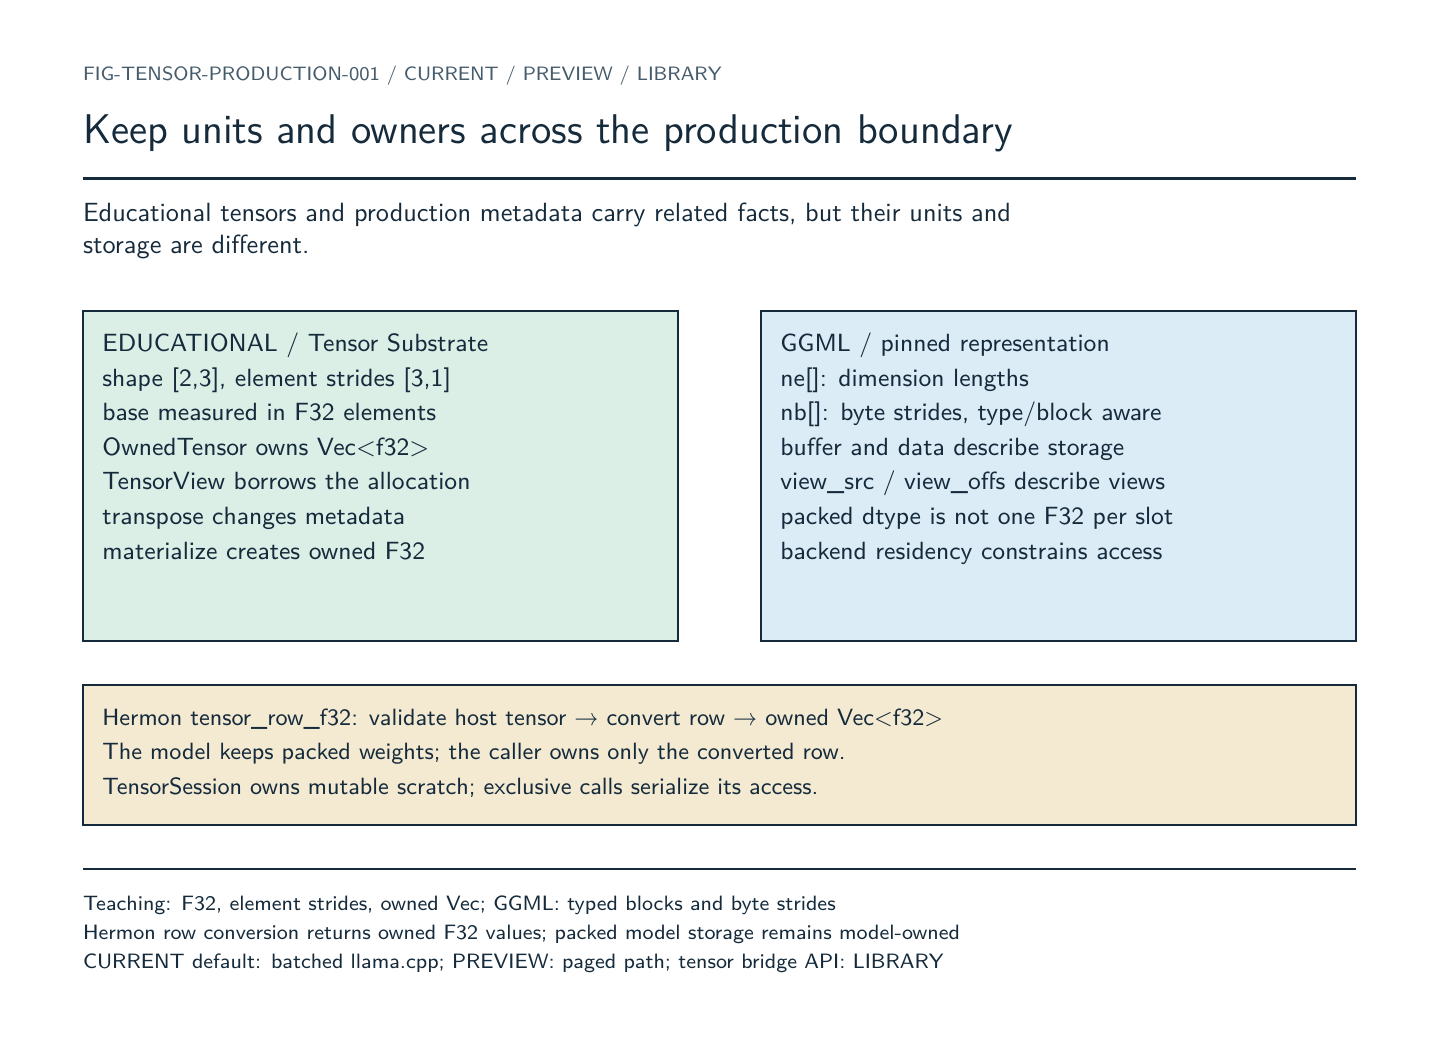
\begin{tikzpicture}[x=.5pt,y=-.5pt]
\path[use as bounding box] (0,0) rectangle (1000,720);
\path[fill=white,draw=none,line width=0.5pt] (0.0,0.0) rectangle (1000.0,720.0);
\node[inner sep=0pt,outer sep=0pt,anchor=base west,text={rgb,255:red,70;green,92;blue,107},font=\sffamily\fontsize{7.0}{8.4}\selectfont] at (40,38) {FIG-TENSOR-PRODUCTION-001  /  CURRENT / PREVIEW / LIBRARY};
\node[inner sep=0pt,outer sep=0pt,anchor=base west,text={rgb,255:red,21;green,43;blue,60},font=\sffamily\fontsize{15.0}{18.0}\selectfont] at (40,84) {Keep units and owners across the production boundary};
\draw[fill=none,draw={rgb,255:red,21;green,43;blue,60},line width=0.75pt] (40,109) -- (960,109);
\node[inner sep=0pt,outer sep=0pt,anchor=base west,text={rgb,255:red,21;green,43;blue,60},font=\sffamily\fontsize{9.5}{11.4}\selectfont] at (40,140) {Educational tensors and production metadata carry related facts, but their units and};
\node[inner sep=0pt,outer sep=0pt,anchor=base west,text={rgb,255:red,21;green,43;blue,60},font=\sffamily\fontsize{9.5}{11.4}\selectfont] at (40,163) {storage are different.};
\path[fill={rgb,255:red,220;green,239;blue,231},draw={rgb,255:red,21;green,43;blue,60},line width=0.7pt] (40.0,205.0) rectangle (470.0,443.0);
\node[inner sep=0pt,outer sep=0pt,anchor=base west,text={rgb,255:red,21;green,43;blue,60},font=\sffamily\fontsize{9.0}{10.799999999999999}\selectfont] at (54,234) {EDUCATIONAL / Tensor Substrate};
\node[inner sep=0pt,outer sep=0pt,anchor=base west,text={rgb,255:red,21;green,43;blue,60},font=\sffamily\fontsize{9.0}{10.799999999999999}\selectfont] at (54,259) {shape [2,3], element strides [3,1]};
\node[inner sep=0pt,outer sep=0pt,anchor=base west,text={rgb,255:red,21;green,43;blue,60},font=\sffamily\fontsize{9.0}{10.799999999999999}\selectfont] at (54,284) {base measured in F32 elements};
\node[inner sep=0pt,outer sep=0pt,anchor=base west,text={rgb,255:red,21;green,43;blue,60},font=\sffamily\fontsize{9.0}{10.799999999999999}\selectfont] at (54,309) {OwnedTensor owns Vec<f32>};
\node[inner sep=0pt,outer sep=0pt,anchor=base west,text={rgb,255:red,21;green,43;blue,60},font=\sffamily\fontsize{9.0}{10.799999999999999}\selectfont] at (54,334) {TensorView borrows the allocation};
\node[inner sep=0pt,outer sep=0pt,anchor=base west,text={rgb,255:red,21;green,43;blue,60},font=\sffamily\fontsize{9.0}{10.799999999999999}\selectfont] at (54,359) {transpose changes metadata};
\node[inner sep=0pt,outer sep=0pt,anchor=base west,text={rgb,255:red,21;green,43;blue,60},font=\sffamily\fontsize{9.0}{10.799999999999999}\selectfont] at (54,384) {materialize creates owned F32};
\path[fill={rgb,255:red,220;green,236;blue,247},draw={rgb,255:red,21;green,43;blue,60},line width=0.7pt] (530.0,205.0) rectangle (960.0,443.0);
\node[inner sep=0pt,outer sep=0pt,anchor=base west,text={rgb,255:red,21;green,43;blue,60},font=\sffamily\fontsize{9.0}{10.799999999999999}\selectfont] at (544,234) {GGML / pinned representation};
\node[inner sep=0pt,outer sep=0pt,anchor=base west,text={rgb,255:red,21;green,43;blue,60},font=\sffamily\fontsize{9.0}{10.799999999999999}\selectfont] at (544,259) {ne[]: dimension lengths};
\node[inner sep=0pt,outer sep=0pt,anchor=base west,text={rgb,255:red,21;green,43;blue,60},font=\sffamily\fontsize{9.0}{10.799999999999999}\selectfont] at (544,284) {nb[]: byte strides, type/block aware};
\node[inner sep=0pt,outer sep=0pt,anchor=base west,text={rgb,255:red,21;green,43;blue,60},font=\sffamily\fontsize{9.0}{10.799999999999999}\selectfont] at (544,309) {buffer and data describe storage};
\node[inner sep=0pt,outer sep=0pt,anchor=base west,text={rgb,255:red,21;green,43;blue,60},font=\sffamily\fontsize{9.0}{10.799999999999999}\selectfont] at (544,334) {view\_src / view\_offs describe views};
\node[inner sep=0pt,outer sep=0pt,anchor=base west,text={rgb,255:red,21;green,43;blue,60},font=\sffamily\fontsize{9.0}{10.799999999999999}\selectfont] at (544,359) {packed dtype is not one F32 per slot};
\node[inner sep=0pt,outer sep=0pt,anchor=base west,text={rgb,255:red,21;green,43;blue,60},font=\sffamily\fontsize{9.0}{10.799999999999999}\selectfont] at (544,384) {backend residency constrains access};
\path[fill={rgb,255:red,244;green,234;blue,210},draw={rgb,255:red,21;green,43;blue,60},line width=0.7pt] (40.0,475.0) rectangle (960.0,576.0);
\node[inner sep=0pt,outer sep=0pt,anchor=base west,text={rgb,255:red,21;green,43;blue,60},font=\sffamily\fontsize{8.5}{10.2}\selectfont] at (54,504) {Hermon tensor\_row\_f32: validate host tensor → convert row → owned Vec<f32>};
\node[inner sep=0pt,outer sep=0pt,anchor=base west,text={rgb,255:red,21;green,43;blue,60},font=\sffamily\fontsize{8.5}{10.2}\selectfont] at (54,529) {The model keeps packed weights; the caller owns only the converted row.};
\node[inner sep=0pt,outer sep=0pt,anchor=base west,text={rgb,255:red,21;green,43;blue,60},font=\sffamily\fontsize{8.5}{10.2}\selectfont] at (54,554) {TensorSession owns mutable scratch; exclusive calls serialize its access.};
\draw[fill=none,draw={rgb,255:red,21;green,43;blue,60},line width=0.75pt] (40,608) -- (960,608);
\node[inner sep=0pt,outer sep=0pt,anchor=base west,text={rgb,255:red,21;green,43;blue,60},font=\sffamily\fontsize{7.5}{9.0}\selectfont] at (40,638) {Teaching: F32, element strides, owned Vec; GGML: typed blocks and byte strides};
\node[inner sep=0pt,outer sep=0pt,anchor=base west,text={rgb,255:red,21;green,43;blue,60},font=\sffamily\fontsize{7.5}{9.0}\selectfont] at (40,659) {Hermon row conversion returns owned F32 values; packed model storage remains model-owned};
\node[inner sep=0pt,outer sep=0pt,anchor=base west,text={rgb,255:red,21;green,43;blue,60},font=\sffamily\fontsize{7.5}{9.0}\selectfont] at (40,680) {CURRENT default: batched llama.cpp; PREVIEW: paged path; tensor bridge API: LIBRARY};
\end{tikzpicture}
}\caption{Educational element strides and production byte-stride metadata require an explicit representation boundary.}\end{figure}

This comparison preserves the useful commonality without implying
identical APIs. Multiplying an F32 element stride by four gives a byte
displacement, but the same shortcut cannot describe arbitrary packed
quantized blocks. Similarly, a returned F32 row is a caller-owned
conversion result, not a Rust slice into packed model storage. The
\href{https://github.com/hermonai/inside-the-llm-engine/blob/astra-visual-rewrite/research/astra/chapter05-regeneration.md}{dated
source review} records the exact wrapper and runtime gates. Source
availability establishes these contracts; it does not establish a new
hardware benchmark or real-model equivalence result.

\subsection{Run the same tensor through every
representation}\label{run-the-same-tensor-through-every-representation}

The chapter's visual fixture is a contract that can fail independently
of the renderer. From the repository root, run:

\begin{verbatim}
python3 scripts/check-tensor-visual-parity.py
cd code/mini-engine
cargo test -p engine0 --test tensor_visual_contract
cargo test -p engine0 --doc
\end{verbatim}

The parity script asks a Rust example to construct the real owner and
call \texttt{transpose}, \texttt{to\_contiguous}, \texttt{reshape\_view}
and \texttt{slice\_axis}. It compares their reported shapes, strides,
bases, logical values and offsets with independent Python row/column
enumeration and the shared figure fixture. A hand-edited caption cannot
make an incorrect trace pass. Pointer and mutation tests then verify
what numbers alone cannot: aliases remain aliases, and copied/cloned
owners remain independent.

\Needspace{12\baselineskip}

{\def\LTcaptype{none} % do not increment counter
\begin{longtable}[]{@{}
  >{\raggedright\arraybackslash}p{(\linewidth - 8\tabcolsep) * \real{0.2000}}
  >{\raggedright\arraybackslash}p{(\linewidth - 8\tabcolsep) * \real{0.2000}}
  >{\raggedright\arraybackslash}p{(\linewidth - 8\tabcolsep) * \real{0.2000}}
  >{\raggedright\arraybackslash}p{(\linewidth - 8\tabcolsep) * \real{0.2000}}
  >{\raggedright\arraybackslash}p{(\linewidth - 8\tabcolsep) * \real{0.2000}}@{}}
\toprule\noalign{}
\begin{minipage}[b]{\linewidth}\raggedright
Representation
\end{minipage} & \begin{minipage}[b]{\linewidth}\raggedright
Shape
\end{minipage} & \begin{minipage}[b]{\linewidth}\raggedright
Element strides
\end{minipage} & \begin{minipage}[b]{\linewidth}\raggedright
Logical values
\end{minipage} & \begin{minipage}[b]{\linewidth}\raggedright
Owner
\end{minipage} \\
\midrule\noalign{}
\endhead
\bottomrule\noalign{}
\endlastfoot
Original A & \texttt{{[}2,3{]}} & \texttt{{[}3,1{]}} &
\texttt{{[}1,2,3,4,5,6{]}} & original \\
Transpose & \texttt{{[}3,2{]}} & \texttt{{[}1,3{]}} &
\texttt{{[}1,4,2,5,3,6{]}} & borrows original \\
Reshape & \texttt{{[}3,2{]}} & \texttt{{[}2,1{]}} &
\texttt{{[}1,2,3,4,5,6{]}} & borrows original \\
Materialized transpose & \texttt{{[}3,2{]}} & \texttt{{[}2,1{]}} &
\texttt{{[}1,4,2,5,3,6{]}} & new independent owner \\
Column slice, base 1 & \texttt{{[}2,2{]}} & \texttt{{[}3,1{]}} &
\texttt{{[}2,3,5,6{]}} & borrows original \\
\end{longtable}
}

This table is the chapter's synthesis: what entered was one allocation;
what we built was several checked interpretations and one explicit copy.
The next operator can now receive a truthful description of every input
it reads.

\subsection{Common mistakes}\label{common-mistakes-4}

\subsubsection{``A tensor is a GPU
object''}\label{a-tensor-is-a-gpu-object}

A tensor is a data/layout abstraction. V1 is entirely CPU-local. A later
provider may place tensor storage on a GPU, but device placement is not
the definition.

\subsubsection{``Tensor means matrix''}\label{tensor-means-matrix}

A matrix is the rank-2 case. Scalars, vectors, and higher-rank arrays
are also tensors under this book's definition.

\subsubsection{``Rank tells me linear
independence''}\label{rank-tells-me-linear-independence}

Tensor rank counts axes. Matrix rank measures a different algebraic
property.

\subsubsection{``Shape defines layout''}\label{shape-defines-layout}

Shape defines logical dimensions. Strides and base offset map those
dimensions to storage. Equal shape does not imply equal storage order.

\subsubsection{``The element count validates a
view''}\label{the-element-count-validates-a-view}

Four strided elements can reach offset 101. Required extent, not count
alone, must fit storage.

\subsubsection{``Strides are always
bytes''}\label{strides-are-always-bytes}

Their unit is an API contract. V1 uses elements; NumPy and GGML expose
bytes. Mixing the two multiplies every address error by dtype width.

\subsubsection{``Reshape and transpose are the
same''}\label{reshape-and-transpose-are-the-same}

Reshape regroups canonical order. Transpose changes which axis step
moves where and often becomes non-contiguous.

\subsubsection{``Transpose always
copies''}\label{transpose-always-copies}

V1 transpose only swaps metadata. An explicit \texttt{to\_contiguous}
performs a copy.

\subsubsection{``Views own their data''}\label{views-own-their-data}

A \texttt{TensorView\textless{}\textquotesingle{}a\textgreater{}} owns
metadata and borrows storage. It cannot outlive the owner. Two views may
alias.

\subsubsection{``A tensor should perform its own
matmul''}\label{a-tensor-should-perform-its-own-matmul}

Tensor is data plus metadata. A matrix multiplication kernel is an
operation with layout, arithmetic, and execution contracts. Chapter 6
keeps them separate.

\subsection{Labs}\label{labs-1}

Labs 16--21 turn each contract into evidence:

\begin{itemize}
\tightlist
\item
  \href{https://github.com/hermonai/inside-the-llm-engine/blob/astra-visual-rewrite/labs/lab-16-offset-by-hand.md}{Lab
  16} derives offsets by hand.
\item
  \href{https://github.com/hermonai/inside-the-llm-engine/blob/astra-visual-rewrite/labs/lab-17-transpose-without-copy.md}{Lab
  17} proves transpose aliases.
\item
  \href{https://github.com/hermonai/inside-the-llm-engine/blob/astra-visual-rewrite/labs/lab-18-reshape-view.md}{Lab
  18} checks no-copy reshape gates.
\item
  \href{https://github.com/hermonai/inside-the-llm-engine/blob/astra-visual-rewrite/labs/lab-19-non-contiguous-copy.md}{Lab
  19} materializes logical order.
\item
  \href{https://github.com/hermonai/inside-the-llm-engine/blob/astra-visual-rewrite/labs/lab-20-break-shape-arithmetic.md}{Lab
  20} attacks size and extent arithmetic.
\item
  \href{https://github.com/hermonai/inside-the-llm-engine/blob/astra-visual-rewrite/labs/lab-21-mutation-and-aliasing.md}{Lab
  21} uses exclusive mutation.
\end{itemize}

Each moves through CHECK, BUILD, BREAK, or EXTEND without adding later
Transformer operators.

\subsection{Exercises}\label{exercises-4}

\begin{enumerate}
\def\labelenumi{\arabic{enumi}.}
\tightlist
\item
  Derive strides for \texttt{{[}5{]}}, \texttt{{[}2,5{]}},
  \texttt{{[}3,2,5{]}}, and \texttt{{[}1,3,1{]}}. State units.
\item
  For shape \texttt{{[}4,3{]}}, slice rows \texttt{1..3}. Derive shape,
  strides, base, and largest reachable offset.
\item
  Give two different stride vectors for shape \texttt{{[}2,2{]}} over
  six storage values. List the logical visit order of each.
\item
  Explain why a zero-stride immutable view is safe to read but cannot be
  the basis of an arbitrary overlapping mutable API.
\item
  Calculate the minimum storage length for shape \texttt{{[}2,2{]}},
  strides \texttt{{[}100,1{]}}, base 7. Identify every overflow check
  the implementation needs.
\item
  Compare \texttt{{[}3,2{]}} reshape and transpose views of
  \texttt{{[}A,B,C,D,E,F{]}}. Which logical index first reveals that
  they differ?
\item
  Explain why \texttt{from\_vec} moves an allocation while
  \texttt{to\_contiguous} copies elements, even though both return an
  owner.
\item
  Design a typed error for a kernel that accepts only canonical rank-2
  input. Which checks belong to the tensor, and which belong to the
  kernel?
\item
  Sketch a safe API that splits a canonical matrix into two
  non-overlapping mutable row ranges. State the proof required before
  returning borrows.
\item
  Predict how element-stride APIs must adapt at an FFI boundary exposing
  byte strides and a packed quantized dtype.
\end{enumerate}

\subsection{What we still have not
built}\label{what-we-still-have-not-built}

Tensor Substrate v1 can describe and safely access data. It cannot
multiply two matrices, normalize an activation, form Q/K/V, encode
position, apply causal attention, run a feed-forward network, or stack
decoder layers. It has no broadcasting, training graph, packed dtype,
model loader, SIMD kernel, or accelerator provider.

Those exclusions are the point. A small substrate lets us audit every
invariant before performance work raises the stakes. We can now
distinguish a data structure error from an operator error and a
mathematical result from its physical traversal cost.

\subsection{Summary}\label{summary-4}

A tensor is not a vector with a suggestive variable name. It is storage
plus shape, layout, dtype, ownership, and lifetime. Rank counts logical
axes. Shape defines their dimensions. Checked products establish element
and byte counts. Strides and a base offset map bounded logical indices
to physical elements.

Owned tensors are canonical row-major \texttt{f32} storage in v1.
Immutable views may carry general non-negative strides and alias their
owner. Reshape borrows only canonical layouts with equal element counts.
Transpose swaps rank-2 metadata. Slices adjust one dimension and base.
\texttt{to\_contiguous} is the visible allocation and copy boundary.
Rust lifetimes prevent dangling views; exclusive borrowing keeps
arbitrary mutable aliasing out of the API. Every external size and
offset operation is checked.

ENGINE-1 now stores its embedding and projection as tensors, yet
produces the same logits and tokens. Representation changed without
changing model semantics. That is the substitution discipline the rest
of the book will need.

Return to the five opening questions. For ENGINE-1's embedding, the
answers are now executable facts: shape \texttt{{[}V,D{]}}; dtype
\texttt{F32}; canonical row-major strides \texttt{{[}D,1{]}}; storage
owned immutably by \texttt{\seqsplit{TinyLanguageModel}}; and views
bounded by a borrow of that model. For a transposed temporary, the shape
and strides change, the owner does not, and the borrow cannot escape.
For a contiguous copy, the logical values remain equal while ownership
and physical ordering change.

That checklist scales. When later chapters introduce activations, packed
model weights, KV blocks, and device buffers, each new representation
must answer the same questions before a kernel touches it. A familiar
equation is not a waiver. Neither is a familiar framework name. Correct
inference begins by making the data contract complete enough that wrong
layout, wrong lifetime, or wrong size cannot masquerade as valid
arithmetic.

\subsection{Chapter 6 preview: matrix
multiplication}\label{chapter-6-preview-matrix-multiplication}

We can represent matrices correctly. We still need to compute

\[
\mathbf{C}=\mathbf{A}\mathbf{B}
\]

without treating the equation as an execution plan. It does not say
where \(A\), \(B\), and \(C\) live, which dimensions agree, which index
changes fastest, how many floating-point operations occur, how many
bytes move, or whether reuse fits a cache.

Chapter 6---\emph{Matrix Multiplication: The Engine Room}---will derive
dot product, matrix-vector multiplication, matrix-matrix multiplication,
loop ordering, operation count, memory traffic, arithmetic intensity,
tiling, reference kernels, and blocked scalar kernels on top of Tensor
Substrate v1. It will be the first chapter that deliberately thinks like
a performance engineer.

\subsection{References}\label{references-2}

\begin{itemize}
\tightlist
\item
  NumPy developers.
  \href{https://numpy.org/doc/stable/reference/generated/numpy.ndarray.html}{\texttt{ndarray}}
  and
  \href{https://numpy.org/doc/stable/reference/generated/numpy.ndarray.strides.html}{\texttt{ndarray.strides}}.
\item
  PyTorch contributors.
  \href{https://docs.pytorch.org/docs/stable/tensor_view.html}{Tensor
  Views},
  \href{https://docs.pytorch.org/docs/stable/generated/torch.Tensor.view.html}{\texttt{Tensor.view}},
  and
  \href{https://docs.pytorch.org/docs/stable/tensor_attributes.html}{Tensor
  Attributes}.
\item
  The Rust Project.
  \href{https://doc.rust-lang.org/stable/reference/types/slice.html}{Slice
  types} and
  \href{https://doc.rust-lang.org/stable/book/ch04-02-references-and-borrowing.html}{References
  and Borrowing}.
\item
  The Rust Project.
  \href{https://doc.rust-lang.org/std/primitive.usize.html\#method.checked_mul}{\texttt{\seqsplit{usize::checked\_mul}}}.
\item
  ggml-org. Pinned
  \href{https://github.com/ggml-org/llama.cpp/blob/389ff61d77b5c71cec0cf92fe4e5d01ace80b797/ggml/include/ggml.h}{\texttt{ggml.h}}.
\item
  Hermon source at commit
  \href{https://github.com/hermonai/hermon/commit/5e908d75e4d5ee102f97f6a880ed4d0968d949df}{\texttt{5e908d7}},
  especially \texttt{hermon-llamacpp}, \texttt{hermon-gguf}, and the
  paged runtime boundary.
\end{itemize}

\clearpage

\section{Chapter 6 --- Matrix Multiplication: The Engine
Room}\label{chapter-6-matrix-multiplication-the-engine-room}

Chapter 5 gave tensor values addresses. Shape said which logical indices
were legal, strides mapped those indices to storage, and ownership said
how long the bytes remained alive. Yet an inference engine exists to
\emph{compute} with those values. Its most familiar numerical operation
is also one of its most consequential systems problems: matrix
multiplication.

A mathematical line such as \(C=AB\) looks atomic. A processor does not
receive that line. It receives loads, multiplications, additions,
stores, branches, and addresses. The same mathematical products can be
visited in different orders. Those orders can move very different
amounts of data through a memory hierarchy, even when their operation
counts are identical.

This chapter builds the book's first optimization cycle:

\begin{center}\begin{adjustbox}{max width=\linewidth}% Legacy topology preserved as native vectors and typeset labels.
\begin{tikzpicture}[x=6.2pt,y=-13pt,draw=black!65,line width=.45pt]
\path[use as bounding box] (-1,-1) rectangle (62,6);
\draw (14,0) -- (13.5,0);
\draw (14,0) -- (14.5,0);
\draw (15,0) -- (14.5,0);
\draw (15,0) -- (15.5,0);
\draw[-{Latex[length=2pt,width=3pt]}] (15.5,0) -- (16.5,0);
\draw (35,0) -- (34.5,0);
\draw (35,0) -- (35.5,0);
\draw (36,0) -- (35.5,0);
\draw (36,0) -- (36.5,0);
\draw[-{Latex[length=2pt,width=3pt]}] (36.5,0) -- (37.5,0);
\node[anchor=west,inner sep=0pt,font=\sffamily\fontsize{9}{11}\selectfont] at (-0.4,0) {\begin{adjustbox}{max width=80.60000000000001pt}specification\end{adjustbox}};
\node[anchor=west,inner sep=0pt,font=\sffamily\fontsize{9}{11}\selectfont] at (17.6,0) {\begin{adjustbox}{max width=99.2pt}reference kernel\end{adjustbox}};
\node[anchor=west,inner sep=0pt,font=\sffamily\fontsize{9}{11}\selectfont] at (38.6,0) {\begin{adjustbox}{max width=136.4pt}optimized substitution\end{adjustbox}};
\draw[-{Latex[length=2pt,width=3pt]}] (6,1.5) -- (6,0.5);
\draw (48,1) -- (48,0.5);
\draw (48,1) -- (48,1.5);
\draw (6,2) -- (6.5,2);
\draw (6,2) -- (6,1.5);
\draw (7,2) -- (6.5,2);
\draw (7,2) -- (7.5,2);
\draw (8,2) -- (7.5,2);
\draw (8,2) -- (8.5,2);
\draw (9,2) -- (8.5,2);
\draw (9,2) -- (9.5,2);
\draw (10,2) -- (9.5,2);
\draw (10,2) -- (10.5,2);
\draw (11,2) -- (10.5,2);
\draw (11,2) -- (11.5,2);
\draw (12,2) -- (11.5,2);
\draw (12,2) -- (12.5,2);
\draw (13,2) -- (12.5,2);
\draw (13,2) -- (13.5,2);
\draw (14,2) -- (13.5,2);
\draw (14,2) -- (14.5,2);
\draw[-{Latex[length=2pt,width=3pt]}] (34.5,2) -- (33.5,2);
\draw (35,2) -- (34.5,2);
\draw (35,2) -- (35.5,2);
\draw (36,2) -- (35.5,2);
\draw (36,2) -- (36.5,2);
\draw (37,2) -- (36.5,2);
\draw (37,2) -- (37.5,2);
\draw (38,2) -- (37.5,2);
\draw (38,2) -- (38.5,2);
\draw (39,2) -- (38.5,2);
\draw (39,2) -- (39.5,2);
\draw (40,2) -- (39.5,2);
\draw (40,2) -- (40.5,2);
\draw (41,2) -- (40.5,2);
\draw (41,2) -- (41.5,2);
\draw (42,2) -- (41.5,2);
\draw (42,2) -- (42.5,2);
\draw (43,2) -- (42.5,2);
\draw (43,2) -- (43.5,2);
\draw (44,2) -- (43.5,2);
\draw (44,2) -- (44.5,2);
\draw (45,2) -- (44.5,2);
\draw (45,2) -- (45.5,2);
\draw (46,2) -- (45.5,2);
\draw (46,2) -- (46.5,2);
\draw (47,2) -- (46.5,2);
\draw (47,2) -- (47.5,2);
\draw (48,2) -- (47.5,2);
\draw (48,2) -- (48,1.5);
\node[anchor=west,inner sep=0pt,font=\sffamily\fontsize{9}{11}\selectfont] at (15.6,2) {\begin{adjustbox}{max width=105.4pt}equivalence proof\end{adjustbox}};
\draw (30,3) -- (30,2.5);
\draw (30,3) -- (30,3.5);
\draw[-{Latex[length=2pt,width=3pt]}] (30,3.5) -- (30,4.5);
\node[anchor=west,inner sep=0pt,font=\sffamily\fontsize{9}{11}\selectfont] at (24.6,5) {\begin{adjustbox}{max width=68.2pt}measurement\end{adjustbox}};
\end{tikzpicture}
\end{adjustbox}\end{center}

The cycle matters more than the particular optimization. ENGINE-2 will
contain an obviously inspectable scalar reference path and a
cache-blocked scalar CPU path. It will keep both. The reference defines
behavior for general valid views; the blocked path accepts a narrower
layout contract and must earn its place with correctness gates and
measurements.

\begin{quote}
\textbf{FIRST PRINCIPLE} Matrix multiplication specifies which values
contribute to an answer. A kernel specifies the order in which
arithmetic and byte movement realize that answer.
\end{quote}

\begin{figure}[H]\centering\resizebox{\linewidth}{!}{% Generated from figures/generated/ch06-engine.svg; do not hand edit.
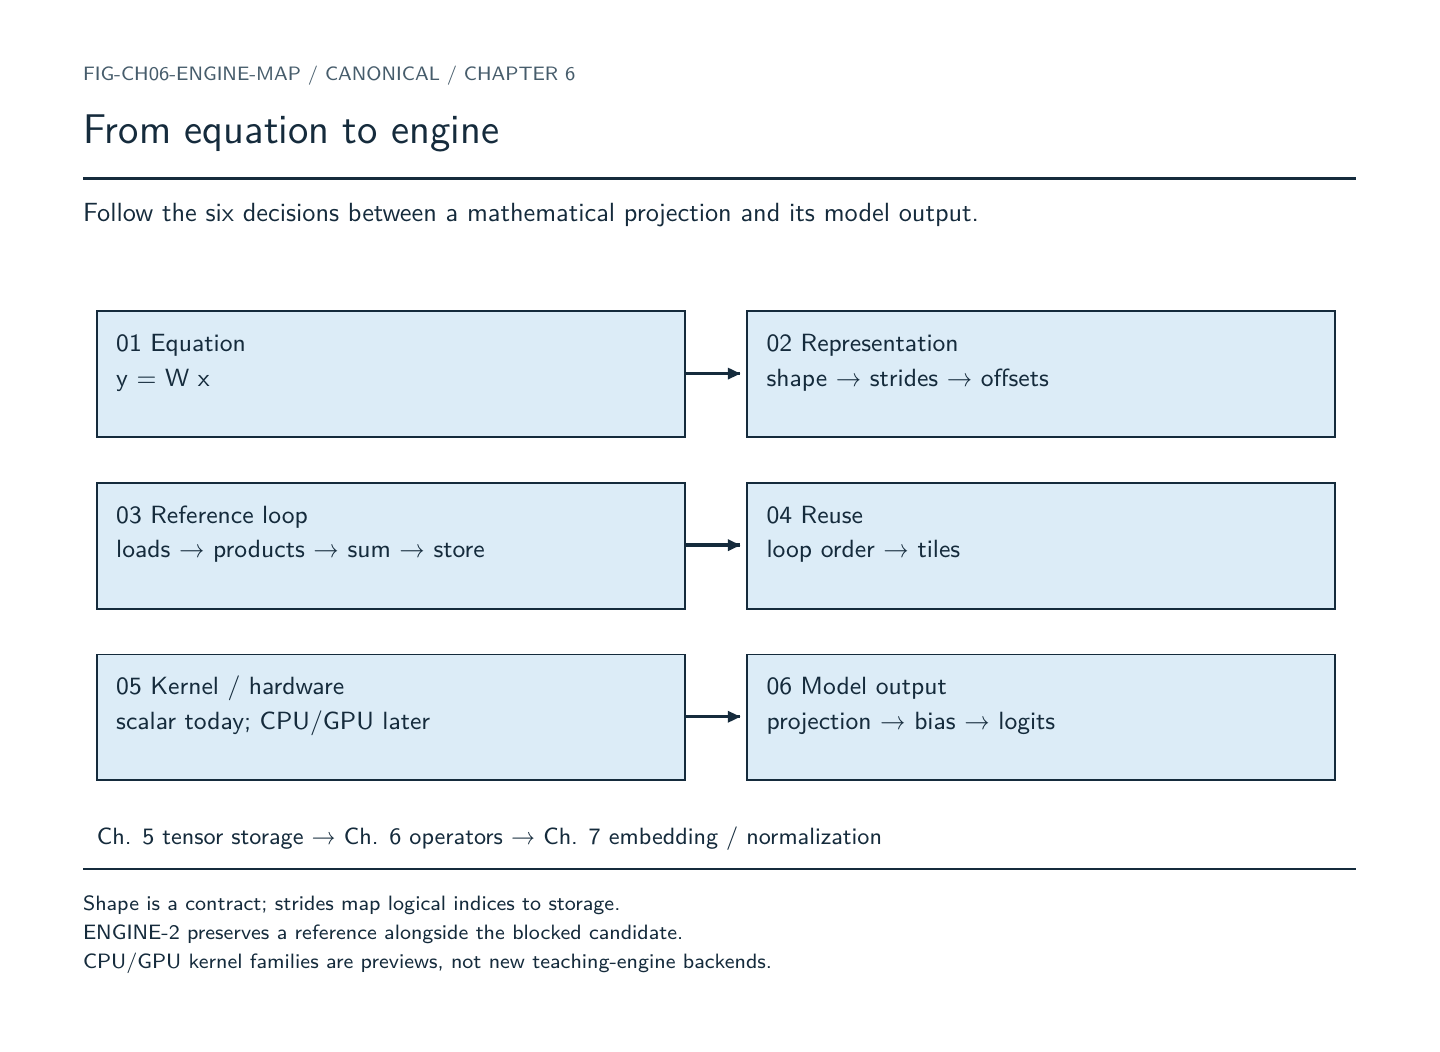
\begin{tikzpicture}[x=.5pt,y=-.5pt]
\path[use as bounding box] (0,0) rectangle (1000,720);
\path[fill=white,draw=none,line width=0.5pt] (0.0,0.0) rectangle (1000.0,720.0);
\node[inner sep=0pt,outer sep=0pt,anchor=base west,text={rgb,255:red,70;green,92;blue,107},font=\sffamily\fontsize{7.0}{8.4}\selectfont] at (40,38) {FIG-CH06-ENGINE-MAP  /  CANONICAL / CHAPTER 6};
\node[inner sep=0pt,outer sep=0pt,anchor=base west,text={rgb,255:red,21;green,43;blue,60},font=\sffamily\fontsize{15.0}{18.0}\selectfont] at (40,84) {From equation to engine};
\draw[fill=none,draw={rgb,255:red,21;green,43;blue,60},line width=0.75pt] (40,109) -- (960,109);
\node[inner sep=0pt,outer sep=0pt,anchor=base west,text={rgb,255:red,21;green,43;blue,60},font=\sffamily\fontsize{9.5}{11.4}\selectfont] at (40,140) {Follow the six decisions between a mathematical projection and its model output.};
\path[fill={rgb,255:red,220;green,236;blue,247},draw={rgb,255:red,21;green,43;blue,60},line width=0.7pt] (50.0,205.0) rectangle (475.0,296.0);
\node[inner sep=0pt,outer sep=0pt,anchor=base west,text={rgb,255:red,21;green,43;blue,60},font=\sffamily\fontsize{9.0}{10.799999999999999}\selectfont] at (64,234) {01  Equation};
\node[inner sep=0pt,outer sep=0pt,anchor=base west,text={rgb,255:red,21;green,43;blue,60},font=\sffamily\fontsize{9.0}{10.799999999999999}\selectfont] at (64,259) {y = W x};
\draw[fill=none,draw={rgb,255:red,21;green,43;blue,60},line width=1.25pt] (475,250) -- (515,250);
\path[fill={rgb,255:red,21;green,43;blue,60},draw=none,line width=0.5pt] (515.00,250.00) -- (506.00,254.35) -- (506.00,245.65) -- cycle;
\path[fill={rgb,255:red,220;green,236;blue,247},draw={rgb,255:red,21;green,43;blue,60},line width=0.7pt] (520.0,205.0) rectangle (945.0,296.0);
\node[inner sep=0pt,outer sep=0pt,anchor=base west,text={rgb,255:red,21;green,43;blue,60},font=\sffamily\fontsize{9.0}{10.799999999999999}\selectfont] at (534,234) {02  Representation};
\node[inner sep=0pt,outer sep=0pt,anchor=base west,text={rgb,255:red,21;green,43;blue,60},font=\sffamily\fontsize{9.0}{10.799999999999999}\selectfont] at (534,259) {shape → strides → offsets};
\path[fill={rgb,255:red,220;green,236;blue,247},draw={rgb,255:red,21;green,43;blue,60},line width=0.7pt] (50.0,329.0) rectangle (475.0,420.0);
\node[inner sep=0pt,outer sep=0pt,anchor=base west,text={rgb,255:red,21;green,43;blue,60},font=\sffamily\fontsize{9.0}{10.799999999999999}\selectfont] at (64,358) {03  Reference loop};
\node[inner sep=0pt,outer sep=0pt,anchor=base west,text={rgb,255:red,21;green,43;blue,60},font=\sffamily\fontsize{9.0}{10.799999999999999}\selectfont] at (64,383) {loads → products → sum → store};
\draw[fill=none,draw={rgb,255:red,21;green,43;blue,60},line width=1.25pt] (475,374) -- (515,374);
\path[fill={rgb,255:red,21;green,43;blue,60},draw=none,line width=0.5pt] (515.00,374.00) -- (506.00,378.35) -- (506.00,369.65) -- cycle;
\path[fill={rgb,255:red,220;green,236;blue,247},draw={rgb,255:red,21;green,43;blue,60},line width=0.7pt] (520.0,329.0) rectangle (945.0,420.0);
\node[inner sep=0pt,outer sep=0pt,anchor=base west,text={rgb,255:red,21;green,43;blue,60},font=\sffamily\fontsize{9.0}{10.799999999999999}\selectfont] at (534,358) {04  Reuse};
\node[inner sep=0pt,outer sep=0pt,anchor=base west,text={rgb,255:red,21;green,43;blue,60},font=\sffamily\fontsize{9.0}{10.799999999999999}\selectfont] at (534,383) {loop order → tiles};
\path[fill={rgb,255:red,220;green,236;blue,247},draw={rgb,255:red,21;green,43;blue,60},line width=0.7pt] (50.0,453.0) rectangle (475.0,544.0);
\node[inner sep=0pt,outer sep=0pt,anchor=base west,text={rgb,255:red,21;green,43;blue,60},font=\sffamily\fontsize{9.0}{10.799999999999999}\selectfont] at (64,482) {05  Kernel / hardware};
\node[inner sep=0pt,outer sep=0pt,anchor=base west,text={rgb,255:red,21;green,43;blue,60},font=\sffamily\fontsize{9.0}{10.799999999999999}\selectfont] at (64,507) {scalar today; CPU/GPU later};
\draw[fill=none,draw={rgb,255:red,21;green,43;blue,60},line width=1.25pt] (475,498) -- (515,498);
\path[fill={rgb,255:red,21;green,43;blue,60},draw=none,line width=0.5pt] (515.00,498.00) -- (506.00,502.35) -- (506.00,493.65) -- cycle;
\path[fill={rgb,255:red,220;green,236;blue,247},draw={rgb,255:red,21;green,43;blue,60},line width=0.7pt] (520.0,453.0) rectangle (945.0,544.0);
\node[inner sep=0pt,outer sep=0pt,anchor=base west,text={rgb,255:red,21;green,43;blue,60},font=\sffamily\fontsize{9.0}{10.799999999999999}\selectfont] at (534,482) {06  Model output};
\node[inner sep=0pt,outer sep=0pt,anchor=base west,text={rgb,255:red,21;green,43;blue,60},font=\sffamily\fontsize{9.0}{10.799999999999999}\selectfont] at (534,507) {projection → bias → logits};
\node[inner sep=0pt,outer sep=0pt,anchor=base west,text={rgb,255:red,21;green,43;blue,60},font=\sffamily\fontsize{8.5}{10.2}\selectfont] at (50,590) {Ch. 5 tensor storage → Ch. 6 operators → Ch. 7 embedding / normalization};
\draw[fill=none,draw={rgb,255:red,21;green,43;blue,60},line width=0.75pt] (40,608) -- (960,608);
\node[inner sep=0pt,outer sep=0pt,anchor=base west,text={rgb,255:red,21;green,43;blue,60},font=\sffamily\fontsize{7.5}{9.0}\selectfont] at (40,638) {Shape is a contract; strides map logical indices to storage.};
\node[inner sep=0pt,outer sep=0pt,anchor=base west,text={rgb,255:red,21;green,43;blue,60},font=\sffamily\fontsize{7.5}{9.0}\selectfont] at (40,659) {ENGINE-2 preserves a reference alongside the blocked candidate.};
\node[inner sep=0pt,outer sep=0pt,anchor=base west,text={rgb,255:red,21;green,43;blue,60},font=\sffamily\fontsize{7.5}{9.0}\selectfont] at (40,680) {CPU/GPU kernel families are previews, not new teaching-engine backends.};
\end{tikzpicture}
}\caption{From equation through addresses, reference loops, reuse, and hardware to model output.}\end{figure}

Read this chapter in three passes: first determine \textbf{which values}
contribute; then trace \textbf{which addresses} the implementation
visits; finally ask \textbf{what the measurements justify}. A fast wrong
answer fails the first pass. A plausible cache story without timing
evidence fails the third. The production comparison at the end
translates these same questions into Hermon and GGML, without adding a
production backend to the teaching engine.

\subsection{The most important loop in
AI}\label{the-most-important-loop-in-ai}

Language-model inference repeatedly applies learned linear
transformations. Later chapters will add normalization, position
handling, attention, and feed-forward networks. Under many of those
operators sit matrix-vector or matrix-matrix products. They project
activations from one feature space into another; they also dominate
large regions of weight storage and execution.

That importance does not make every product the same. During one-token
decode, a weight matrix may multiply one activation vector. During work
over several tokens or requests, the same weights may multiply several
columns or rows of activations. The equations are closely related, but
their opportunity to reuse each weight after loading it is different.
Shape is therefore part of the performance problem, not merely a type
check.

ENGINE-1 already contained a linear projection:

\[
\mathbf{z}=\mathbf{W}\mathbf{h}+\mathbf{b},
\]

where \(\mathbf{W}\in\mathbb{R}^{V_{\mathrm{vocab}}\times D}\),
\(\mathbf{h}\in\mathbb{R}^{D}\),
\(\mathbf{b}\in\mathbb{R}^{V_{\mathrm{vocab}}}\), and
\(\mathbf{z}\in\mathbb{R}^{V_{\mathrm{vocab}}}\). The old implementation
spelled the matrix-vector product as loops inside the model. That was
appropriate when the loop first made logits real. It is now duplication.
Chapter 6 extracts the numerical operation into a kernel layer while
leaving embedding lookup and bias addition as explicit model operations.

\subsection{From multiply to
multiply-accumulate}\label{from-multiply-to-multiply-accumulate}

Begin with one multiplication. Given two \texttt{f32} values \(a\) and
\(b\), their product contributes \(ab\) to some destination. A linear
algebra kernel rarely needs that product alone. It adds many products
into an accumulator:

\[
s \leftarrow s + ab.
\]

This is a multiply-accumulate step. Hardware may later implement the
expression with a fused multiply-add instruction, which rounds once
rather than rounding the product and sum separately. ENGINE-2 does not
select intrinsics or promise fused behavior. Its source uses
\texttt{f32} operands and an \texttt{f32} accumulator. The independent
oracle models separate \texttt{f32} rounding, while cross-path tests use
an explicit tolerance so compiler and architecture choices cannot
masquerade as semantic failure.

Follow one contribution in the canonical
\href{https://github.com/hermonai/inside-the-llm-engine/blob/astra-visual-rewrite/diagrams/linear/follow-the-flop.txt}{FLOP
diagram}:

\begin{center}\begin{adjustbox}{max width=\linewidth}% Legacy topology preserved as native vectors and typeset labels.
\begin{tikzpicture}[x=6.2pt,y=-13pt,draw=black!65,line width=.45pt]
\path[use as bounding box] (-1,-1) rectangle (39,8);
\node[anchor=west,inner sep=0pt,font=\sffamily\fontsize{9}{11}\selectfont] at (0.6,0) {\begin{adjustbox}{max width=18.6pt}Aᵢₖ\end{adjustbox}};
\node[anchor=west,inner sep=0pt,font=\sffamily\fontsize{9}{11}\selectfont] at (21.6,0) {\begin{adjustbox}{max width=18.6pt}Bₖⱼ\end{adjustbox}};
\draw (2,1) -- (2,0.5);
\draw (2,1) -- (2,1.5);
\draw (23,1) -- (23,0.5);
\draw (23,1) -- (23,1.5);
\draw (2,2) -- (2.5,2);
\draw (2,2) -- (2,1.5);
\draw (3,2) -- (2.5,2);
\draw (3,2) -- (3.5,2);
\draw (4,2) -- (3.5,2);
\draw (4,2) -- (4.5,2);
\draw (5,2) -- (4.5,2);
\draw (5,2) -- (5.5,2);
\draw (6,2) -- (5.5,2);
\draw (6,2) -- (6.5,2);
\draw (7,2) -- (6.5,2);
\draw (7,2) -- (7.5,2);
\draw (8,2) -- (7.5,2);
\draw (8,2) -- (8.5,2);
\draw (9,2) -- (8.5,2);
\draw (9,2) -- (9.5,2);
\draw (10,2) -- (9.5,2);
\draw (10,2) -- (10.5,2);
\draw (11,2) -- (10.5,2);
\draw (11,2) -- (11.5,2);
\draw (12,2) -- (11.5,2);
\draw (12,2) -- (12.5,2);
\draw (13,2) -- (12.5,2);
\draw (13,2) -- (13.5,2);
\draw (13,2) -- (13,2.5);
\draw (14,2) -- (13.5,2);
\draw (14,2) -- (14.5,2);
\draw (15,2) -- (14.5,2);
\draw (15,2) -- (15.5,2);
\draw (16,2) -- (15.5,2);
\draw (16,2) -- (16.5,2);
\draw (17,2) -- (16.5,2);
\draw (17,2) -- (17.5,2);
\draw (18,2) -- (17.5,2);
\draw (18,2) -- (18.5,2);
\draw (19,2) -- (18.5,2);
\draw (19,2) -- (19.5,2);
\draw (20,2) -- (19.5,2);
\draw (20,2) -- (20.5,2);
\draw (21,2) -- (20.5,2);
\draw (21,2) -- (21.5,2);
\draw (22,2) -- (21.5,2);
\draw (22,2) -- (22.5,2);
\draw (23,2) -- (22.5,2);
\draw (23,2) -- (23,1.5);
\draw[-{Latex[length=2pt,width=3pt]}] (13,2.5) -- (13,3.5);
\node[anchor=west,inner sep=0pt,font=\sffamily\fontsize{9}{11}\selectfont] at (7.6,4) {\begin{adjustbox}{max width=74.4pt}f32 multiply\end{adjustbox}};
\draw (13,5) -- (13,4.5);
\draw (13,5) -- (13,5.5);
\draw[-{Latex[length=2pt,width=3pt]}] (13,5.5) -- (13,6.5);
\draw (14,7) -- (13.5,7);
\draw (14,7) -- (14.5,7);
\draw (15,7) -- (14.5,7);
\draw (15,7) -- (15.5,7);
\draw[-{Latex[length=2pt,width=3pt]}] (15.5,7) -- (16.5,7);
\draw (26,7) -- (25.5,7);
\draw (26,7) -- (26.5,7);
\draw (27,7) -- (26.5,7);
\draw (27,7) -- (27.5,7);
\draw[-{Latex[length=2pt,width=3pt]}] (27.5,7) -- (28.5,7);
\node[anchor=west,inner sep=0pt,font=\sffamily\fontsize{9}{11}\selectfont] at (0.6,7) {\begin{adjustbox}{max width=74.4pt}previous Cᵢⱼ\end{adjustbox}};
\node[anchor=west,inner sep=0pt,font=\sffamily\fontsize{9}{11}\selectfont] at (17.6,7) {\begin{adjustbox}{max width=43.4pt}f32 add\end{adjustbox}};
\node[anchor=west,inner sep=0pt,font=\sffamily\fontsize{9}{11}\selectfont] at (29.6,7) {\begin{adjustbox}{max width=49.6pt}next Cᵢⱼ\end{adjustbox}};
\end{tikzpicture}
\end{adjustbox}\end{center}

The floating-point representation makes the update bounded in precision,
not exact over real numbers; overflow can produce infinity. If large
positive and negative contributions nearly cancel, rounding error can be
visible. If an optimized kernel changes the reduction order, its final
low bits may change as well.

\subsection{Dot product}\label{dot-product}

For two vectors \(\mathbf{a},\mathbf{b}\in\mathbb{R}^{K}\), the dot
product is

\[
\mathbf{a}\cdot\mathbf{b}
=\sum_{k=0}^{K-1}a_kb_k.
\]

For the chapter's canonical example, take \(\mathbf{a}=[1,-2,3,0]\) and
\(\mathbf{x}=[2,1,-1,0.5]\):

\[
\mathbf{a}\cdot\mathbf{x}
=1(2)+(-2)(1)+3(-1)+0(0.5)
=2-2-3+0=-3.
\]

\begin{figure}[H]\centering\resizebox{\linewidth}{!}{% Generated from figures/generated/ch06-dot.svg; do not hand edit.
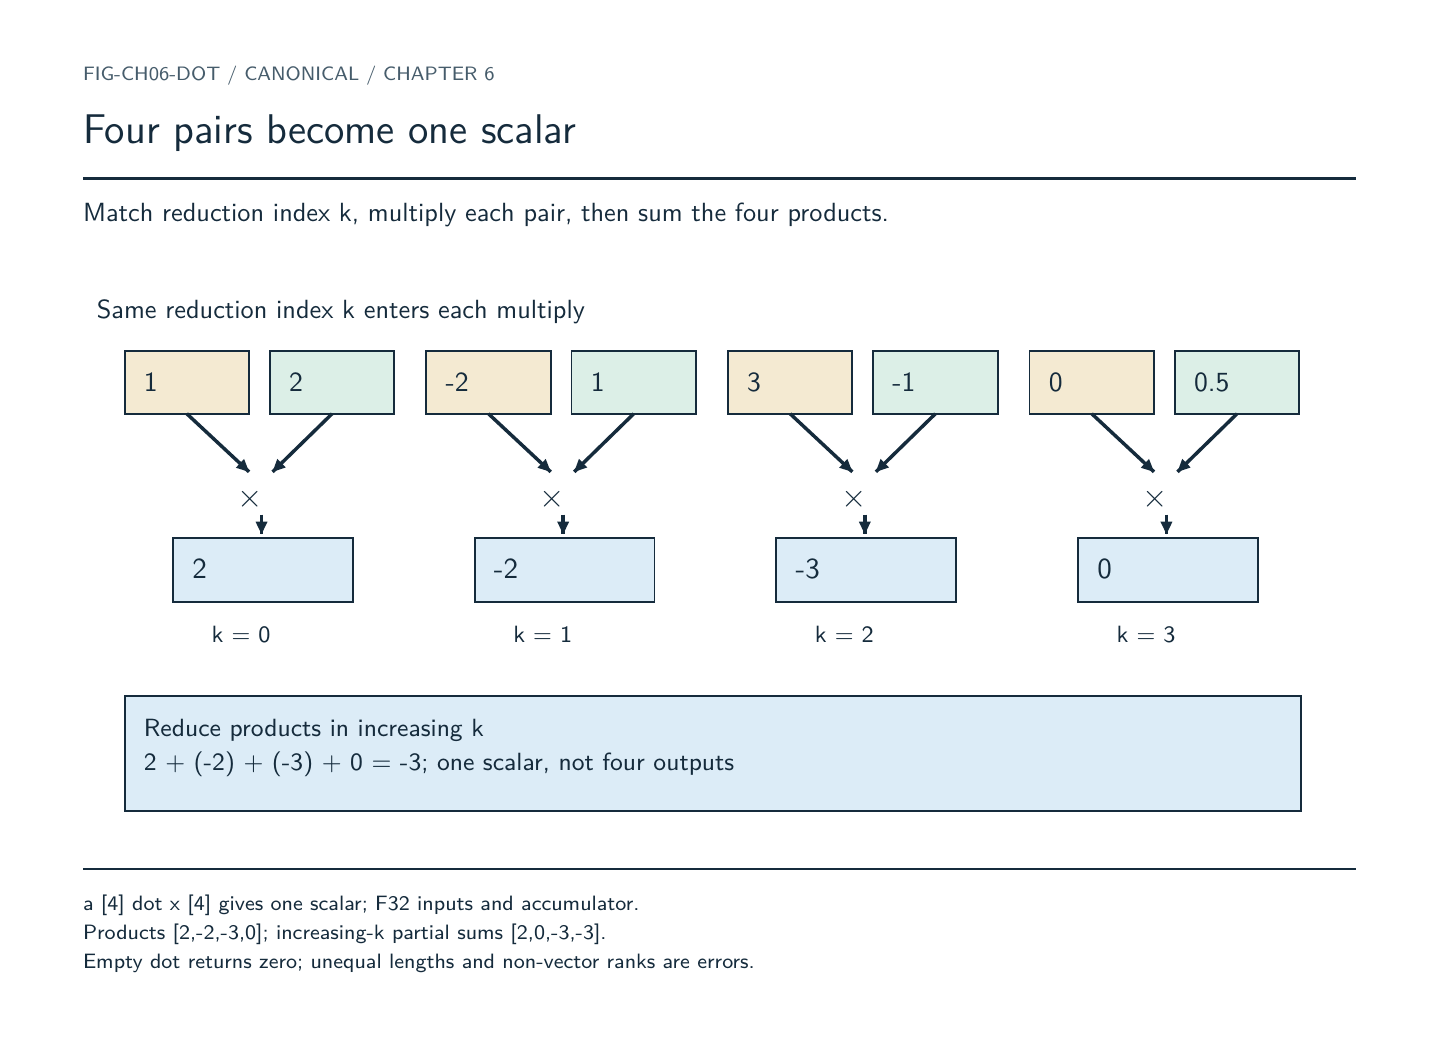
\begin{tikzpicture}[x=.5pt,y=-.5pt]
\path[use as bounding box] (0,0) rectangle (1000,720);
\path[fill=white,draw=none,line width=0.5pt] (0.0,0.0) rectangle (1000.0,720.0);
\node[inner sep=0pt,outer sep=0pt,anchor=base west,text={rgb,255:red,70;green,92;blue,107},font=\sffamily\fontsize{7.0}{8.4}\selectfont] at (40,38) {FIG-CH06-DOT  /  CANONICAL / CHAPTER 6};
\node[inner sep=0pt,outer sep=0pt,anchor=base west,text={rgb,255:red,21;green,43;blue,60},font=\sffamily\fontsize{15.0}{18.0}\selectfont] at (40,84) {Four pairs become one scalar};
\draw[fill=none,draw={rgb,255:red,21;green,43;blue,60},line width=0.75pt] (40,109) -- (960,109);
\node[inner sep=0pt,outer sep=0pt,anchor=base west,text={rgb,255:red,21;green,43;blue,60},font=\sffamily\fontsize{9.5}{11.4}\selectfont] at (40,140) {Match reduction index k, multiply each pair, then sum the four products.};
\node[inner sep=0pt,outer sep=0pt,anchor=base west,text={rgb,255:red,21;green,43;blue,60},font=\sffamily\fontsize{9.5}{11.4}\selectfont] at (50,210) {Same reduction index k enters each multiply};
\path[fill={rgb,255:red,244;green,234;blue,210},draw={rgb,255:red,21;green,43;blue,60},line width=0.7pt] (70.0,234.0) rectangle (160.0,279.0);
\node[inner sep=0pt,outer sep=0pt,anchor=base west,text={rgb,255:red,21;green,43;blue,60},font=\sffamily\fontsize{10.0}{12.0}\selectfont] at (84,263) {1};
\path[fill={rgb,255:red,220;green,239;blue,231},draw={rgb,255:red,21;green,43;blue,60},line width=0.7pt] (175.0,234.0) rectangle (265.0,279.0);
\node[inner sep=0pt,outer sep=0pt,anchor=base west,text={rgb,255:red,21;green,43;blue,60},font=\sffamily\fontsize{10.0}{12.0}\selectfont] at (189,263) {2};
\draw[fill=none,draw={rgb,255:red,21;green,43;blue,60},line width=1.25pt] (115,279) -- (160,321);
\path[fill={rgb,255:red,21;green,43;blue,60},draw=none,line width=0.5pt] (160.00,321.00) -- (150.45,318.04) -- (156.39,311.68) -- cycle;
\draw[fill=none,draw={rgb,255:red,21;green,43;blue,60},line width=1.25pt] (220,279) -- (177,321);
\path[fill={rgb,255:red,21;green,43;blue,60},draw=none,line width=0.5pt] (177.00,321.00) -- (180.40,311.60) -- (186.48,317.82) -- cycle;
\node[inner sep=0pt,outer sep=0pt,anchor=base west,text={rgb,255:red,21;green,43;blue,60},font=\sffamily\fontsize{12.0}{14.399999999999999}\selectfont] at (152,347) {×};
\draw[fill=none,draw={rgb,255:red,21;green,43;blue,60},line width=1.25pt] (169,352) -- (169,366);
\path[fill={rgb,255:red,21;green,43;blue,60},draw=none,line width=0.5pt] (169.00,366.00) -- (164.65,357.00) -- (173.35,357.00) -- cycle;
\path[fill={rgb,255:red,220;green,236;blue,247},draw={rgb,255:red,21;green,43;blue,60},line width=0.7pt] (105.0,369.0) rectangle (235.0,415.0);
\node[inner sep=0pt,outer sep=0pt,anchor=base west,text={rgb,255:red,21;green,43;blue,60},font=\sffamily\fontsize{10.5}{12.6}\selectfont] at (119,398) {2};
\node[inner sep=0pt,outer sep=0pt,anchor=base west,text={rgb,255:red,21;green,43;blue,60},font=\sffamily\fontsize{8.5}{10.2}\selectfont] at (133,444) {k = 0};
\path[fill={rgb,255:red,244;green,234;blue,210},draw={rgb,255:red,21;green,43;blue,60},line width=0.7pt] (288.0,234.0) rectangle (378.0,279.0);
\node[inner sep=0pt,outer sep=0pt,anchor=base west,text={rgb,255:red,21;green,43;blue,60},font=\sffamily\fontsize{10.0}{12.0}\selectfont] at (302,263) {-2};
\path[fill={rgb,255:red,220;green,239;blue,231},draw={rgb,255:red,21;green,43;blue,60},line width=0.7pt] (393.0,234.0) rectangle (483.0,279.0);
\node[inner sep=0pt,outer sep=0pt,anchor=base west,text={rgb,255:red,21;green,43;blue,60},font=\sffamily\fontsize{10.0}{12.0}\selectfont] at (407,263) {1};
\draw[fill=none,draw={rgb,255:red,21;green,43;blue,60},line width=1.25pt] (333,279) -- (378,321);
\path[fill={rgb,255:red,21;green,43;blue,60},draw=none,line width=0.5pt] (378.00,321.00) -- (368.45,318.04) -- (374.39,311.68) -- cycle;
\draw[fill=none,draw={rgb,255:red,21;green,43;blue,60},line width=1.25pt] (438,279) -- (395,321);
\path[fill={rgb,255:red,21;green,43;blue,60},draw=none,line width=0.5pt] (395.00,321.00) -- (398.40,311.60) -- (404.48,317.82) -- cycle;
\node[inner sep=0pt,outer sep=0pt,anchor=base west,text={rgb,255:red,21;green,43;blue,60},font=\sffamily\fontsize{12.0}{14.399999999999999}\selectfont] at (370,347) {×};
\draw[fill=none,draw={rgb,255:red,21;green,43;blue,60},line width=1.25pt] (387,352) -- (387,366);
\path[fill={rgb,255:red,21;green,43;blue,60},draw=none,line width=0.5pt] (387.00,366.00) -- (382.65,357.00) -- (391.35,357.00) -- cycle;
\path[fill={rgb,255:red,220;green,236;blue,247},draw={rgb,255:red,21;green,43;blue,60},line width=0.7pt] (323.0,369.0) rectangle (453.0,415.0);
\node[inner sep=0pt,outer sep=0pt,anchor=base west,text={rgb,255:red,21;green,43;blue,60},font=\sffamily\fontsize{10.5}{12.6}\selectfont] at (337,398) {-2};
\node[inner sep=0pt,outer sep=0pt,anchor=base west,text={rgb,255:red,21;green,43;blue,60},font=\sffamily\fontsize{8.5}{10.2}\selectfont] at (351,444) {k = 1};
\path[fill={rgb,255:red,244;green,234;blue,210},draw={rgb,255:red,21;green,43;blue,60},line width=0.7pt] (506.0,234.0) rectangle (596.0,279.0);
\node[inner sep=0pt,outer sep=0pt,anchor=base west,text={rgb,255:red,21;green,43;blue,60},font=\sffamily\fontsize{10.0}{12.0}\selectfont] at (520,263) {3};
\path[fill={rgb,255:red,220;green,239;blue,231},draw={rgb,255:red,21;green,43;blue,60},line width=0.7pt] (611.0,234.0) rectangle (701.0,279.0);
\node[inner sep=0pt,outer sep=0pt,anchor=base west,text={rgb,255:red,21;green,43;blue,60},font=\sffamily\fontsize{10.0}{12.0}\selectfont] at (625,263) {-1};
\draw[fill=none,draw={rgb,255:red,21;green,43;blue,60},line width=1.25pt] (551,279) -- (596,321);
\path[fill={rgb,255:red,21;green,43;blue,60},draw=none,line width=0.5pt] (596.00,321.00) -- (586.45,318.04) -- (592.39,311.68) -- cycle;
\draw[fill=none,draw={rgb,255:red,21;green,43;blue,60},line width=1.25pt] (656,279) -- (613,321);
\path[fill={rgb,255:red,21;green,43;blue,60},draw=none,line width=0.5pt] (613.00,321.00) -- (616.40,311.60) -- (622.48,317.82) -- cycle;
\node[inner sep=0pt,outer sep=0pt,anchor=base west,text={rgb,255:red,21;green,43;blue,60},font=\sffamily\fontsize{12.0}{14.399999999999999}\selectfont] at (588,347) {×};
\draw[fill=none,draw={rgb,255:red,21;green,43;blue,60},line width=1.25pt] (605,352) -- (605,366);
\path[fill={rgb,255:red,21;green,43;blue,60},draw=none,line width=0.5pt] (605.00,366.00) -- (600.65,357.00) -- (609.35,357.00) -- cycle;
\path[fill={rgb,255:red,220;green,236;blue,247},draw={rgb,255:red,21;green,43;blue,60},line width=0.7pt] (541.0,369.0) rectangle (671.0,415.0);
\node[inner sep=0pt,outer sep=0pt,anchor=base west,text={rgb,255:red,21;green,43;blue,60},font=\sffamily\fontsize{10.5}{12.6}\selectfont] at (555,398) {-3};
\node[inner sep=0pt,outer sep=0pt,anchor=base west,text={rgb,255:red,21;green,43;blue,60},font=\sffamily\fontsize{8.5}{10.2}\selectfont] at (569,444) {k = 2};
\path[fill={rgb,255:red,244;green,234;blue,210},draw={rgb,255:red,21;green,43;blue,60},line width=0.7pt] (724.0,234.0) rectangle (814.0,279.0);
\node[inner sep=0pt,outer sep=0pt,anchor=base west,text={rgb,255:red,21;green,43;blue,60},font=\sffamily\fontsize{10.0}{12.0}\selectfont] at (738,263) {0};
\path[fill={rgb,255:red,220;green,239;blue,231},draw={rgb,255:red,21;green,43;blue,60},line width=0.7pt] (829.0,234.0) rectangle (919.0,279.0);
\node[inner sep=0pt,outer sep=0pt,anchor=base west,text={rgb,255:red,21;green,43;blue,60},font=\sffamily\fontsize{10.0}{12.0}\selectfont] at (843,263) {0.5};
\draw[fill=none,draw={rgb,255:red,21;green,43;blue,60},line width=1.25pt] (769,279) -- (814,321);
\path[fill={rgb,255:red,21;green,43;blue,60},draw=none,line width=0.5pt] (814.00,321.00) -- (804.45,318.04) -- (810.39,311.68) -- cycle;
\draw[fill=none,draw={rgb,255:red,21;green,43;blue,60},line width=1.25pt] (874,279) -- (831,321);
\path[fill={rgb,255:red,21;green,43;blue,60},draw=none,line width=0.5pt] (831.00,321.00) -- (834.40,311.60) -- (840.48,317.82) -- cycle;
\node[inner sep=0pt,outer sep=0pt,anchor=base west,text={rgb,255:red,21;green,43;blue,60},font=\sffamily\fontsize{12.0}{14.399999999999999}\selectfont] at (806,347) {×};
\draw[fill=none,draw={rgb,255:red,21;green,43;blue,60},line width=1.25pt] (823,352) -- (823,366);
\path[fill={rgb,255:red,21;green,43;blue,60},draw=none,line width=0.5pt] (823.00,366.00) -- (818.65,357.00) -- (827.35,357.00) -- cycle;
\path[fill={rgb,255:red,220;green,236;blue,247},draw={rgb,255:red,21;green,43;blue,60},line width=0.7pt] (759.0,369.0) rectangle (889.0,415.0);
\node[inner sep=0pt,outer sep=0pt,anchor=base west,text={rgb,255:red,21;green,43;blue,60},font=\sffamily\fontsize{10.5}{12.6}\selectfont] at (773,398) {0};
\node[inner sep=0pt,outer sep=0pt,anchor=base west,text={rgb,255:red,21;green,43;blue,60},font=\sffamily\fontsize{8.5}{10.2}\selectfont] at (787,444) {k = 3};
\path[fill={rgb,255:red,220;green,236;blue,247},draw={rgb,255:red,21;green,43;blue,60},line width=0.7pt] (70.0,483.0) rectangle (920.0,566.0);
\node[inner sep=0pt,outer sep=0pt,anchor=base west,text={rgb,255:red,21;green,43;blue,60},font=\sffamily\fontsize{9.0}{10.799999999999999}\selectfont] at (84,512) {Reduce products in increasing k};
\node[inner sep=0pt,outer sep=0pt,anchor=base west,text={rgb,255:red,21;green,43;blue,60},font=\sffamily\fontsize{9.0}{10.799999999999999}\selectfont] at (84,537) {2 + (-2) + (-3) + 0 = -3; one scalar, not four outputs};
\draw[fill=none,draw={rgb,255:red,21;green,43;blue,60},line width=0.75pt] (40,608) -- (960,608);
\node[inner sep=0pt,outer sep=0pt,anchor=base west,text={rgb,255:red,21;green,43;blue,60},font=\sffamily\fontsize{7.5}{9.0}\selectfont] at (40,638) {a [4] dot x [4] gives one scalar; F32 inputs and accumulator.};
\node[inner sep=0pt,outer sep=0pt,anchor=base west,text={rgb,255:red,21;green,43;blue,60},font=\sffamily\fontsize{7.5}{9.0}\selectfont] at (40,659) {Products [2,-2,-3,0]; increasing-k partial sums [2,0,-3,-3].};
\node[inner sep=0pt,outer sep=0pt,anchor=base west,text={rgb,255:red,21;green,43;blue,60},font=\sffamily\fontsize{7.5}{9.0}\selectfont] at (40,680) {Empty dot returns zero; unequal lengths and non-vector ranks are errors.};
\end{tikzpicture}
}\caption{Four matched-index products reduce to one scalar, minus three.}\end{figure}

The two operands enter each multiplication independently. The product at
index 2 is \(3(-1)\), never \(3(0.5)\): matching the reduction index is
the operation's identity. A visually pleasing crossing arrow that pairs
the wrong indices would teach a different computation.

The
\href{https://github.com/hermonai/inside-the-llm-engine/blob/astra-visual-rewrite/diagrams/linear/dot-product-multiply-accumulate.txt}{multiply-accumulate
diagram} shows the reduction visually. The shape contract is strict:
both operands have tensor rank 1 and the same length \(K\). ENGINE-2
does not silently truncate to the shorter length or broadcast one
element.

When \(K=0\), the loop has no terms. The sum is the additive identity,
zero. This is not a special numerical trick; it is the standard
empty-sum convention and makes zero-dimensional matrix products
composable.

\subsection{Build it: scalar dot}\label{build-it-scalar-dot}

The reference implementation is deliberately direct:

\begin{verbatim}
let mut sum = 0.0_f32;
for index in 0..left_len {
    sum += *left.get(&[index])? * *right.get(&[index])?;
}
\end{verbatim}

Validation happens before the loop. \texttt{TensorView::get} then
follows each operand's logical indexing contract. A stride-2 vector and
a zero-stride read-only broadcast view are therefore valid. The kernel
is not assuming that logical neighbors occupy adjacent storage.

\begin{quote}
\textbf{BUILD IT} Complete
\href{https://github.com/hermonai/inside-the-llm-engine/blob/astra-visual-rewrite/labs/lab-22-dot-product.md}{Lab
22}. Expand the arithmetic, run \texttt{dot\_reference}, then demand
typed failures for bad rank and length.
\end{quote}

This function is not meant to beat a tuned vector library. It gives
later kernels a legible semantic anchor: one reduction, ordered from
index 0 through \(K-1\), into \texttt{f32}.

\subsection{Matrix times vector}\label{matrix-times-vector}

Let \(\mathbf{A}\in\mathbb{R}^{M\times K}\) and
\(\mathbf{x}\in\mathbb{R}^{K}\). Their matrix-vector product
\(\mathbf{y}=\mathbf{A}\mathbf{x}\in\mathbb{R}^{M}\) has one dot product
per matrix row:

\[
y_i=\sum_{k=0}^{K-1}A_{ik}x_k,
\qquad 0\le i<M.
\]

The shared \(K\) dimension is contracted. The \(M\) row dimension
survives into the output. The complete
\href{https://github.com/hermonai/inside-the-llm-engine/blob/astra-visual-rewrite/diagrams/linear/gemv-shape-contract.txt}{GEMV
shape diagram} makes that flow explicit.

Use one rectangular fixture throughout the numerical plates. We call the
weight matrix \(W\) here and use \(A=W\) when discussing generic GEMM:

\[
W=
\begin{bmatrix}
1&-2&3&0\\
0&1&-1&2\\
2&0&1&-1
\end{bmatrix},
\qquad
\mathbf{x}=
\begin{bmatrix}
2\\1\\-1\\0.5
\end{bmatrix},
\]

the first row produces

\[
y_0=1(2)+(-2)(1)+3(-1)+0(0.5)=-3,
\]

while the remaining rows produce

\[
\begin{aligned}
y_1&=0(2)+1(1)+(-1)(-1)+2(0.5)=3,\\
y_2&=2(2)+0(1)+1(-1)+(-1)(0.5)=2.5.
\end{aligned}
\]

Thus \(\mathbf{y}=[-3,3,2.5]\). The rectangular matrix and mixed signs
help expose orientation errors that square, all-positive fixtures can
conceal.

\begin{figure}[H]\centering\resizebox{\linewidth}{!}{% Generated from figures/generated/ch06-row.svg; do not hand edit.
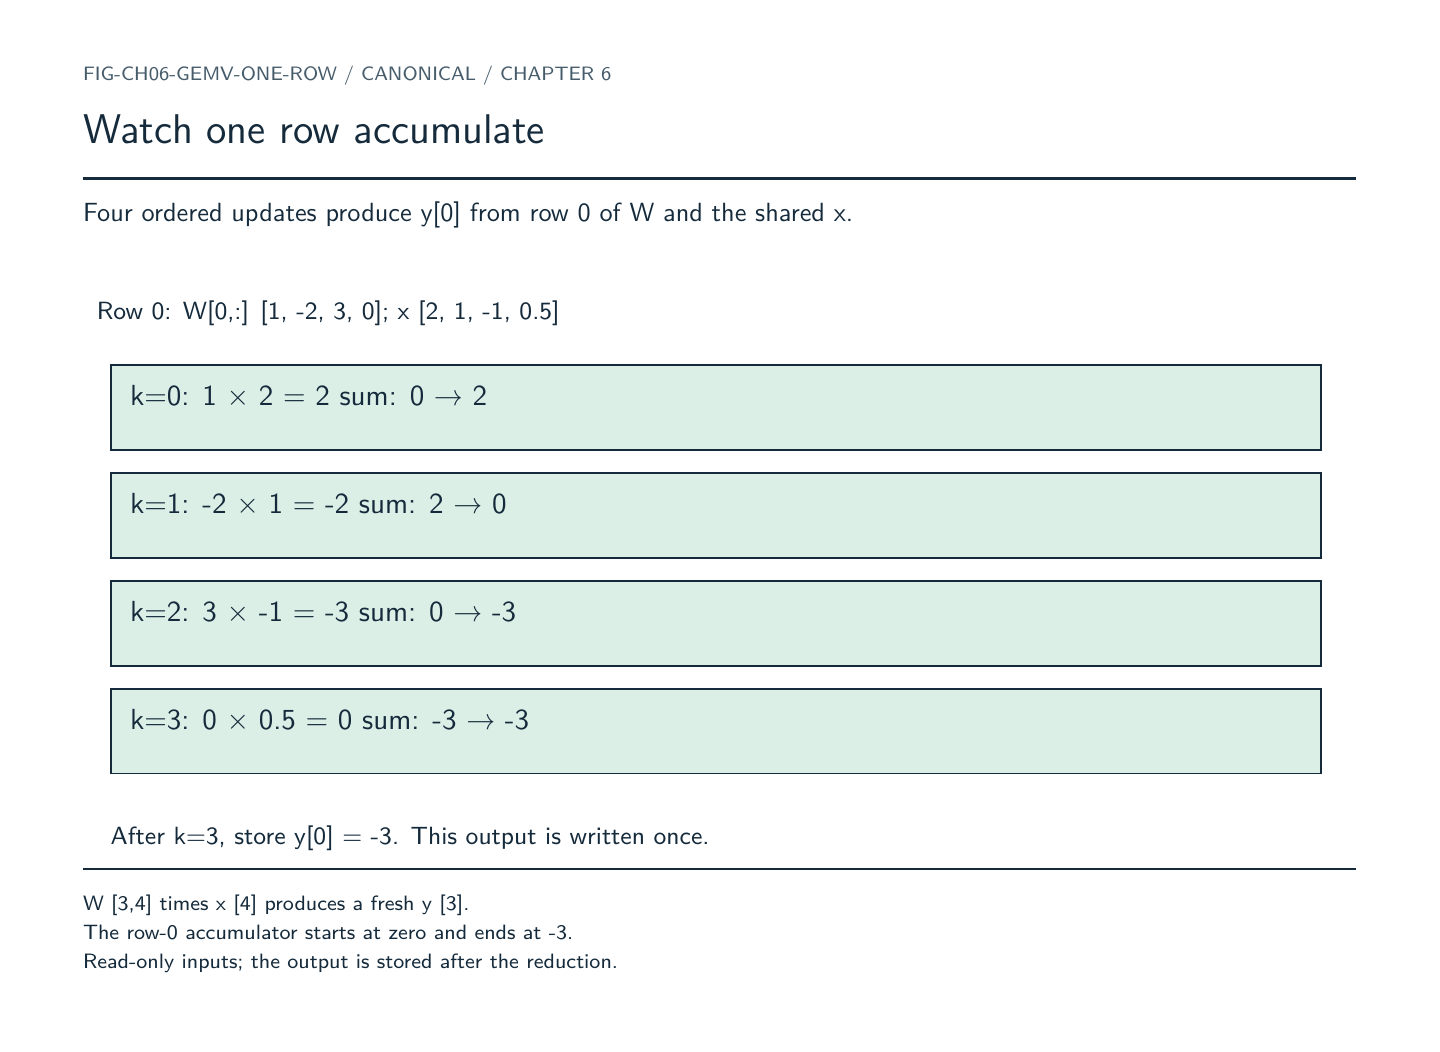
\begin{tikzpicture}[x=.5pt,y=-.5pt]
\path[use as bounding box] (0,0) rectangle (1000,720);
\path[fill=white,draw=none,line width=0.5pt] (0.0,0.0) rectangle (1000.0,720.0);
\node[inner sep=0pt,outer sep=0pt,anchor=base west,text={rgb,255:red,70;green,92;blue,107},font=\sffamily\fontsize{7.0}{8.4}\selectfont] at (40,38) {FIG-CH06-GEMV-ONE-ROW  /  CANONICAL / CHAPTER 6};
\node[inner sep=0pt,outer sep=0pt,anchor=base west,text={rgb,255:red,21;green,43;blue,60},font=\sffamily\fontsize{15.0}{18.0}\selectfont] at (40,84) {Watch one row accumulate};
\draw[fill=none,draw={rgb,255:red,21;green,43;blue,60},line width=0.75pt] (40,109) -- (960,109);
\node[inner sep=0pt,outer sep=0pt,anchor=base west,text={rgb,255:red,21;green,43;blue,60},font=\sffamily\fontsize{9.5}{11.4}\selectfont] at (40,140) {Four ordered updates produce y[0] from row 0 of W and the shared x.};
\node[inner sep=0pt,outer sep=0pt,anchor=base west,text={rgb,255:red,21;green,43;blue,60},font=\sffamily\fontsize{9.0}{10.799999999999999}\selectfont] at (50,211) {Row 0: W[0,:] [1, -2, 3, 0]; x [2, 1, -1, 0.5]};
\path[fill={rgb,255:red,220;green,239;blue,231},draw={rgb,255:red,21;green,43;blue,60},line width=0.7pt] (60.0,244.0) rectangle (935.0,305.0);
\node[inner sep=0pt,outer sep=0pt,anchor=base west,text={rgb,255:red,21;green,43;blue,60},font=\sffamily\fontsize{10.5}{12.6}\selectfont] at (74,273) {k=0:  1 × 2 = 2     sum: 0 → 2};
\path[fill={rgb,255:red,220;green,239;blue,231},draw={rgb,255:red,21;green,43;blue,60},line width=0.7pt] (60.0,322.0) rectangle (935.0,383.0);
\node[inner sep=0pt,outer sep=0pt,anchor=base west,text={rgb,255:red,21;green,43;blue,60},font=\sffamily\fontsize{10.5}{12.6}\selectfont] at (74,351) {k=1:  -2 × 1 = -2     sum: 2 → 0};
\path[fill={rgb,255:red,220;green,239;blue,231},draw={rgb,255:red,21;green,43;blue,60},line width=0.7pt] (60.0,400.0) rectangle (935.0,461.0);
\node[inner sep=0pt,outer sep=0pt,anchor=base west,text={rgb,255:red,21;green,43;blue,60},font=\sffamily\fontsize{10.5}{12.6}\selectfont] at (74,429) {k=2:  3 × -1 = -3     sum: 0 → -3};
\path[fill={rgb,255:red,220;green,239;blue,231},draw={rgb,255:red,21;green,43;blue,60},line width=0.7pt] (60.0,478.0) rectangle (935.0,539.0);
\node[inner sep=0pt,outer sep=0pt,anchor=base west,text={rgb,255:red,21;green,43;blue,60},font=\sffamily\fontsize{10.5}{12.6}\selectfont] at (74,507) {k=3:  0 × 0.5 = 0     sum: -3 → -3};
\node[inner sep=0pt,outer sep=0pt,anchor=base west,text={rgb,255:red,21;green,43;blue,60},font=\sffamily\fontsize{9.0}{10.799999999999999}\selectfont] at (60,590) {After k=3, store y[0] = -3. This output is written once.};
\draw[fill=none,draw={rgb,255:red,21;green,43;blue,60},line width=0.75pt] (40,608) -- (960,608);
\node[inner sep=0pt,outer sep=0pt,anchor=base west,text={rgb,255:red,21;green,43;blue,60},font=\sffamily\fontsize{7.5}{9.0}\selectfont] at (40,638) {W [3,4] times x [4] produces a fresh y [3].};
\node[inner sep=0pt,outer sep=0pt,anchor=base west,text={rgb,255:red,21;green,43;blue,60},font=\sffamily\fontsize{7.5}{9.0}\selectfont] at (40,659) {The row-0 accumulator starts at zero and ends at -3.};
\node[inner sep=0pt,outer sep=0pt,anchor=base west,text={rgb,255:red,21;green,43;blue,60},font=\sffamily\fontsize{7.5}{9.0}\selectfont] at (40,680) {Read-only inputs; the output is stored after the reduction.};
\end{tikzpicture}
}\caption{Four increasing-k accumulator states end at y zero equals minus three.}\end{figure}

The partial sums are \(2,0,-3,-3\), starting from zero before the first
product. The final zero product still occupies a legitimate reduction
index. The
\href{https://github.com/hermonai/inside-the-llm-engine/blob/astra-visual-rewrite/figures/generated/ch06-row.html}{step-through
row animation} highlights each update; this static plate contains every
state and loses no information in print. Nothing starts moving
automatically.

\begin{figure}[H]\centering\resizebox{\linewidth}{!}{% Generated from figures/generated/ch06-gemv.svg; do not hand edit.
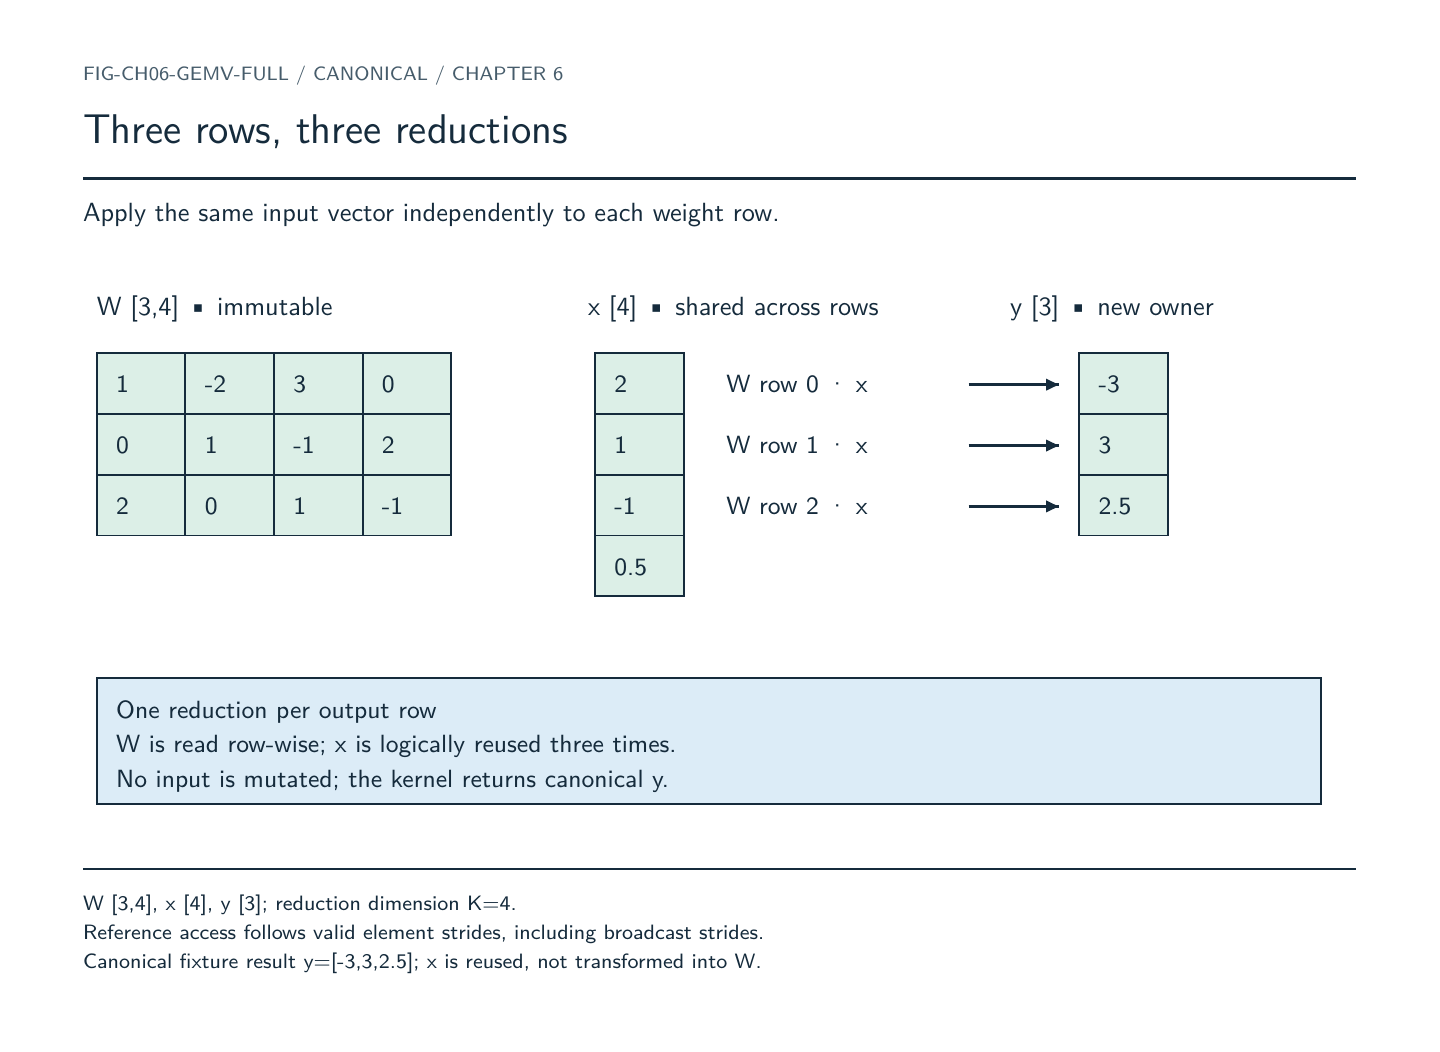
\begin{tikzpicture}[x=.5pt,y=-.5pt]
\path[use as bounding box] (0,0) rectangle (1000,720);
\path[fill=white,draw=none,line width=0.5pt] (0.0,0.0) rectangle (1000.0,720.0);
\node[inner sep=0pt,outer sep=0pt,anchor=base west,text={rgb,255:red,70;green,92;blue,107},font=\sffamily\fontsize{7.0}{8.4}\selectfont] at (40,38) {FIG-CH06-GEMV-FULL  /  CANONICAL / CHAPTER 6};
\node[inner sep=0pt,outer sep=0pt,anchor=base west,text={rgb,255:red,21;green,43;blue,60},font=\sffamily\fontsize{15.0}{18.0}\selectfont] at (40,84) {Three rows, three reductions};
\draw[fill=none,draw={rgb,255:red,21;green,43;blue,60},line width=0.75pt] (40,109) -- (960,109);
\node[inner sep=0pt,outer sep=0pt,anchor=base west,text={rgb,255:red,21;green,43;blue,60},font=\sffamily\fontsize{9.5}{11.4}\selectfont] at (40,140) {Apply the same input vector independently to each weight row.};
\node[inner sep=0pt,outer sep=0pt,anchor=base west,text={rgb,255:red,21;green,43;blue,60},font=\sffamily\fontsize{9.5}{11.4}\selectfont] at (50,208) {W [3,4] • immutable};
\path[fill={rgb,255:red,220;green,239;blue,231},draw={rgb,255:red,21;green,43;blue,60},line width=0.7pt] (50.0,235.0) rectangle (114.0,279.0);
\node[inner sep=0pt,outer sep=0pt,anchor=base west,text={rgb,255:red,21;green,43;blue,60},font=\sffamily\fontsize{9.0}{10.799999999999999}\selectfont] at (64,264) {1};
\path[fill={rgb,255:red,220;green,239;blue,231},draw={rgb,255:red,21;green,43;blue,60},line width=0.7pt] (114.0,235.0) rectangle (178.0,279.0);
\node[inner sep=0pt,outer sep=0pt,anchor=base west,text={rgb,255:red,21;green,43;blue,60},font=\sffamily\fontsize{9.0}{10.799999999999999}\selectfont] at (128,264) {-2};
\path[fill={rgb,255:red,220;green,239;blue,231},draw={rgb,255:red,21;green,43;blue,60},line width=0.7pt] (178.0,235.0) rectangle (242.0,279.0);
\node[inner sep=0pt,outer sep=0pt,anchor=base west,text={rgb,255:red,21;green,43;blue,60},font=\sffamily\fontsize{9.0}{10.799999999999999}\selectfont] at (192,264) {3};
\path[fill={rgb,255:red,220;green,239;blue,231},draw={rgb,255:red,21;green,43;blue,60},line width=0.7pt] (242.0,235.0) rectangle (306.0,279.0);
\node[inner sep=0pt,outer sep=0pt,anchor=base west,text={rgb,255:red,21;green,43;blue,60},font=\sffamily\fontsize{9.0}{10.799999999999999}\selectfont] at (256,264) {0};
\path[fill={rgb,255:red,220;green,239;blue,231},draw={rgb,255:red,21;green,43;blue,60},line width=0.7pt] (50.0,279.0) rectangle (114.0,323.0);
\node[inner sep=0pt,outer sep=0pt,anchor=base west,text={rgb,255:red,21;green,43;blue,60},font=\sffamily\fontsize{9.0}{10.799999999999999}\selectfont] at (64,308) {0};
\path[fill={rgb,255:red,220;green,239;blue,231},draw={rgb,255:red,21;green,43;blue,60},line width=0.7pt] (114.0,279.0) rectangle (178.0,323.0);
\node[inner sep=0pt,outer sep=0pt,anchor=base west,text={rgb,255:red,21;green,43;blue,60},font=\sffamily\fontsize{9.0}{10.799999999999999}\selectfont] at (128,308) {1};
\path[fill={rgb,255:red,220;green,239;blue,231},draw={rgb,255:red,21;green,43;blue,60},line width=0.7pt] (178.0,279.0) rectangle (242.0,323.0);
\node[inner sep=0pt,outer sep=0pt,anchor=base west,text={rgb,255:red,21;green,43;blue,60},font=\sffamily\fontsize{9.0}{10.799999999999999}\selectfont] at (192,308) {-1};
\path[fill={rgb,255:red,220;green,239;blue,231},draw={rgb,255:red,21;green,43;blue,60},line width=0.7pt] (242.0,279.0) rectangle (306.0,323.0);
\node[inner sep=0pt,outer sep=0pt,anchor=base west,text={rgb,255:red,21;green,43;blue,60},font=\sffamily\fontsize{9.0}{10.799999999999999}\selectfont] at (256,308) {2};
\path[fill={rgb,255:red,220;green,239;blue,231},draw={rgb,255:red,21;green,43;blue,60},line width=0.7pt] (50.0,323.0) rectangle (114.0,367.0);
\node[inner sep=0pt,outer sep=0pt,anchor=base west,text={rgb,255:red,21;green,43;blue,60},font=\sffamily\fontsize{9.0}{10.799999999999999}\selectfont] at (64,352) {2};
\path[fill={rgb,255:red,220;green,239;blue,231},draw={rgb,255:red,21;green,43;blue,60},line width=0.7pt] (114.0,323.0) rectangle (178.0,367.0);
\node[inner sep=0pt,outer sep=0pt,anchor=base west,text={rgb,255:red,21;green,43;blue,60},font=\sffamily\fontsize{9.0}{10.799999999999999}\selectfont] at (128,352) {0};
\path[fill={rgb,255:red,220;green,239;blue,231},draw={rgb,255:red,21;green,43;blue,60},line width=0.7pt] (178.0,323.0) rectangle (242.0,367.0);
\node[inner sep=0pt,outer sep=0pt,anchor=base west,text={rgb,255:red,21;green,43;blue,60},font=\sffamily\fontsize{9.0}{10.799999999999999}\selectfont] at (192,352) {1};
\path[fill={rgb,255:red,220;green,239;blue,231},draw={rgb,255:red,21;green,43;blue,60},line width=0.7pt] (242.0,323.0) rectangle (306.0,367.0);
\node[inner sep=0pt,outer sep=0pt,anchor=base west,text={rgb,255:red,21;green,43;blue,60},font=\sffamily\fontsize{9.0}{10.799999999999999}\selectfont] at (256,352) {-1};
\node[inner sep=0pt,outer sep=0pt,anchor=base west,text={rgb,255:red,21;green,43;blue,60},font=\sffamily\fontsize{9.5}{11.4}\selectfont] at (405,208) {x [4] • shared across rows};
\path[fill={rgb,255:red,220;green,239;blue,231},draw={rgb,255:red,21;green,43;blue,60},line width=0.7pt] (410.0,235.0) rectangle (474.0,279.0);
\node[inner sep=0pt,outer sep=0pt,anchor=base west,text={rgb,255:red,21;green,43;blue,60},font=\sffamily\fontsize{9.0}{10.799999999999999}\selectfont] at (424,264) {2};
\path[fill={rgb,255:red,220;green,239;blue,231},draw={rgb,255:red,21;green,43;blue,60},line width=0.7pt] (410.0,279.0) rectangle (474.0,323.0);
\node[inner sep=0pt,outer sep=0pt,anchor=base west,text={rgb,255:red,21;green,43;blue,60},font=\sffamily\fontsize{9.0}{10.799999999999999}\selectfont] at (424,308) {1};
\path[fill={rgb,255:red,220;green,239;blue,231},draw={rgb,255:red,21;green,43;blue,60},line width=0.7pt] (410.0,323.0) rectangle (474.0,367.0);
\node[inner sep=0pt,outer sep=0pt,anchor=base west,text={rgb,255:red,21;green,43;blue,60},font=\sffamily\fontsize{9.0}{10.799999999999999}\selectfont] at (424,352) {-1};
\path[fill={rgb,255:red,220;green,239;blue,231},draw={rgb,255:red,21;green,43;blue,60},line width=0.7pt] (410.0,367.0) rectangle (474.0,411.0);
\node[inner sep=0pt,outer sep=0pt,anchor=base west,text={rgb,255:red,21;green,43;blue,60},font=\sffamily\fontsize{9.0}{10.799999999999999}\selectfont] at (424,396) {0.5};
\node[inner sep=0pt,outer sep=0pt,anchor=base west,text={rgb,255:red,21;green,43;blue,60},font=\sffamily\fontsize{9.5}{11.4}\selectfont] at (710,208) {y [3] • new owner};
\path[fill={rgb,255:red,220;green,239;blue,231},draw={rgb,255:red,21;green,43;blue,60},line width=0.7pt] (760.0,235.0) rectangle (824.0,279.0);
\node[inner sep=0pt,outer sep=0pt,anchor=base west,text={rgb,255:red,21;green,43;blue,60},font=\sffamily\fontsize{9.0}{10.799999999999999}\selectfont] at (774,264) {-3};
\path[fill={rgb,255:red,220;green,239;blue,231},draw={rgb,255:red,21;green,43;blue,60},line width=0.7pt] (760.0,279.0) rectangle (824.0,323.0);
\node[inner sep=0pt,outer sep=0pt,anchor=base west,text={rgb,255:red,21;green,43;blue,60},font=\sffamily\fontsize{9.0}{10.799999999999999}\selectfont] at (774,308) {3};
\path[fill={rgb,255:red,220;green,239;blue,231},draw={rgb,255:red,21;green,43;blue,60},line width=0.7pt] (760.0,323.0) rectangle (824.0,367.0);
\node[inner sep=0pt,outer sep=0pt,anchor=base west,text={rgb,255:red,21;green,43;blue,60},font=\sffamily\fontsize{9.0}{10.799999999999999}\selectfont] at (774,352) {2.5};
\node[inner sep=0pt,outer sep=0pt,anchor=base west,text={rgb,255:red,21;green,43;blue,60},font=\sffamily\fontsize{9.0}{10.799999999999999}\selectfont] at (505,264) {W row 0 · x};
\draw[fill=none,draw={rgb,255:red,21;green,43;blue,60},line width=1.25pt] (680,258) -- (745,258);
\path[fill={rgb,255:red,21;green,43;blue,60},draw=none,line width=0.5pt] (745.00,258.00) -- (736.00,262.35) -- (736.00,253.65) -- cycle;
\node[inner sep=0pt,outer sep=0pt,anchor=base west,text={rgb,255:red,21;green,43;blue,60},font=\sffamily\fontsize{9.0}{10.799999999999999}\selectfont] at (505,308) {W row 1 · x};
\draw[fill=none,draw={rgb,255:red,21;green,43;blue,60},line width=1.25pt] (680,302) -- (745,302);
\path[fill={rgb,255:red,21;green,43;blue,60},draw=none,line width=0.5pt] (745.00,302.00) -- (736.00,306.35) -- (736.00,297.65) -- cycle;
\node[inner sep=0pt,outer sep=0pt,anchor=base west,text={rgb,255:red,21;green,43;blue,60},font=\sffamily\fontsize{9.0}{10.799999999999999}\selectfont] at (505,352) {W row 2 · x};
\draw[fill=none,draw={rgb,255:red,21;green,43;blue,60},line width=1.25pt] (680,346) -- (745,346);
\path[fill={rgb,255:red,21;green,43;blue,60},draw=none,line width=0.5pt] (745.00,346.00) -- (736.00,350.35) -- (736.00,341.65) -- cycle;
\path[fill={rgb,255:red,220;green,236;blue,247},draw={rgb,255:red,21;green,43;blue,60},line width=0.7pt] (50.0,470.0) rectangle (935.0,561.0);
\node[inner sep=0pt,outer sep=0pt,anchor=base west,text={rgb,255:red,21;green,43;blue,60},font=\sffamily\fontsize{9.0}{10.799999999999999}\selectfont] at (64,499) {One reduction per output row};
\node[inner sep=0pt,outer sep=0pt,anchor=base west,text={rgb,255:red,21;green,43;blue,60},font=\sffamily\fontsize{9.0}{10.799999999999999}\selectfont] at (64,524) {W is read row-wise; x is logically reused three times.};
\node[inner sep=0pt,outer sep=0pt,anchor=base west,text={rgb,255:red,21;green,43;blue,60},font=\sffamily\fontsize{9.0}{10.799999999999999}\selectfont] at (64,549) {No input is mutated; the kernel returns canonical y.};
\draw[fill=none,draw={rgb,255:red,21;green,43;blue,60},line width=0.75pt] (40,608) -- (960,608);
\node[inner sep=0pt,outer sep=0pt,anchor=base west,text={rgb,255:red,21;green,43;blue,60},font=\sffamily\fontsize{7.5}{9.0}\selectfont] at (40,638) {W [3,4], x [4], y [3]; reduction dimension K=4.};
\node[inner sep=0pt,outer sep=0pt,anchor=base west,text={rgb,255:red,21;green,43;blue,60},font=\sffamily\fontsize{7.5}{9.0}\selectfont] at (40,659) {Reference access follows valid element strides, including broadcast strides.};
\node[inner sep=0pt,outer sep=0pt,anchor=base west,text={rgb,255:red,21;green,43;blue,60},font=\sffamily\fontsize{7.5}{9.0}\selectfont] at (40,680) {Canonical fixture result y=[-3,3,2.5]; x is reused, not transformed into W.};
\end{tikzpicture}
}\caption{The same x contributes independently to three row dot products and three output values.}\end{figure}

\subsection{Build it: GEMV}\label{build-it-gemv}

\texttt{gemv\_reference} accepts a rank-2 matrix view and a rank-1
vector view. It validates \(A.shape[1]=x.shape[0]\), allocates a new
canonical \texttt{{[}M{]}} \texttt{OwnedTensor}, and fills it with row
dot products. Inputs remain immutable and borrowed; output storage
belongs to the caller.

The ownership choice is important. Returning a view into a temporary
work buffer would entangle result lifetime with kernel internals.
Mutating an input as an output would introduce aliasing questions. A
fresh owner makes the v1 contract simple:

\begin{center}\begin{adjustbox}{max width=\linewidth}% Legacy topology preserved as native vectors and typeset labels.
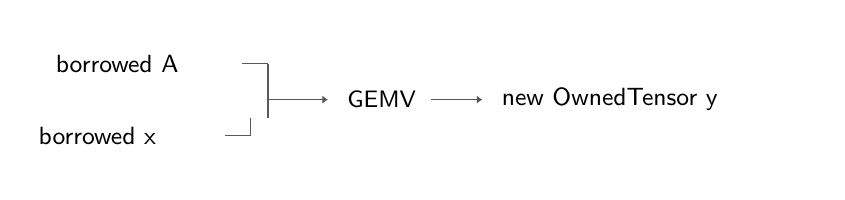
\begin{tikzpicture}[x=6.2pt,y=-13pt,draw=black!65,line width=.45pt]
\path[use as bounding box] (-1,-1) rectangle (45,3);
\draw (12,0) -- (11.5,0);
\draw (12,0) -- (12.5,0);
\draw (13,0) -- (12.5,0);
\draw (13,0) -- (13,0.5);
\node[anchor=west,inner sep=0pt,font=\sffamily\fontsize{9}{11}\selectfont] at (0.6,0) {\begin{adjustbox}{max width=62.0pt}borrowed A\end{adjustbox}};
\draw (13,1) -- (13,0.5);
\draw (13,1) -- (13.5,1);
\draw (13,1) -- (13,1.5);
\draw (14,1) -- (13.5,1);
\draw (14,1) -- (14.5,1);
\draw (15,1) -- (14.5,1);
\draw (15,1) -- (15.5,1);
\draw[-{Latex[length=2pt,width=3pt]}] (15.5,1) -- (16.5,1);
\draw (23,1) -- (22.5,1);
\draw (23,1) -- (23.5,1);
\draw (24,1) -- (23.5,1);
\draw (24,1) -- (24.5,1);
\draw[-{Latex[length=2pt,width=3pt]}] (24.5,1) -- (25.5,1);
\node[anchor=west,inner sep=0pt,font=\sffamily\fontsize{9}{11}\selectfont] at (17.6,1) {\begin{adjustbox}{max width=24.8pt}GEMV\end{adjustbox}};
\node[anchor=west,inner sep=0pt,font=\sffamily\fontsize{9}{11}\selectfont] at (26.6,1) {\begin{adjustbox}{max width=105.4pt}new OwnedTensor y\end{adjustbox}};
\draw (11,2) -- (10.5,2);
\draw (11,2) -- (11.5,2);
\draw (12,2) -- (11.5,2);
\draw (12,2) -- (12,1.5);
\node[anchor=west,inner sep=0pt,font=\sffamily\fontsize{9}{11}\selectfont] at (-0.4,2) {\begin{adjustbox}{max width=62.0pt}borrowed x\end{adjustbox}};
\end{tikzpicture}
\end{adjustbox}\end{center}

The numerical body is the existing kernel, not a diagram-only
implementation:

\begin{verbatim}
for (row, value) in output.iter_mut().enumerate() {
    let mut sum = 0.0_f32;
    for k in 0..inner {
        sum += *matrix.get2(row, k)? * *vector.get(&[k])?;
    }
    *value = sum;
}
\end{verbatim}

For shape \texttt{{[}M,0{]}\ ×\ {[}0{]}}, the result is an owned
\texttt{{[}M{]}} vector of zeros. For \texttt{{[}0,K{]}\ ×\ {[}K{]}}, it
is an empty owner with shape \texttt{{[}0{]}}. No sentinel or fallback
path is needed.

\begin{quote}
\textbf{BUILD IT} Complete
\href{https://github.com/hermonai/inside-the-llm-engine/blob/astra-visual-rewrite/labs/lab-23-gemv-by-hand.md}{Lab
23}, including the strided fixture. Physical padding must not affect the
logical result.
\end{quote}

\subsection{From a weight coordinate to a loaded
F32}\label{from-a-weight-coordinate-to-a-loaded-f32}

Chapter 5's address contract remains active inside every multiply. For a
valid rank-2 view with element strides \(s_0,s_1\) and base offset
\(o\),

\[
\operatorname{offset}_W(i,k)=o+i s_0+k s_1.
\]

Our canonical \(W:[3,4]\) has strides \texttt{{[}4,1{]}} and base zero.
Therefore \(W_{1,2}\) lives at element \(1(4)+2=6\), whose displacement
from the allocation's start is \(4(6)=24\) bytes for F32. The loaded
value is \(-1\). An element index, a byte displacement, and the value at
that location are three different things.

\begin{figure}[H]\centering\resizebox{\linewidth}{!}{% Generated from figures/generated/ch06-memory.svg; do not hand edit.
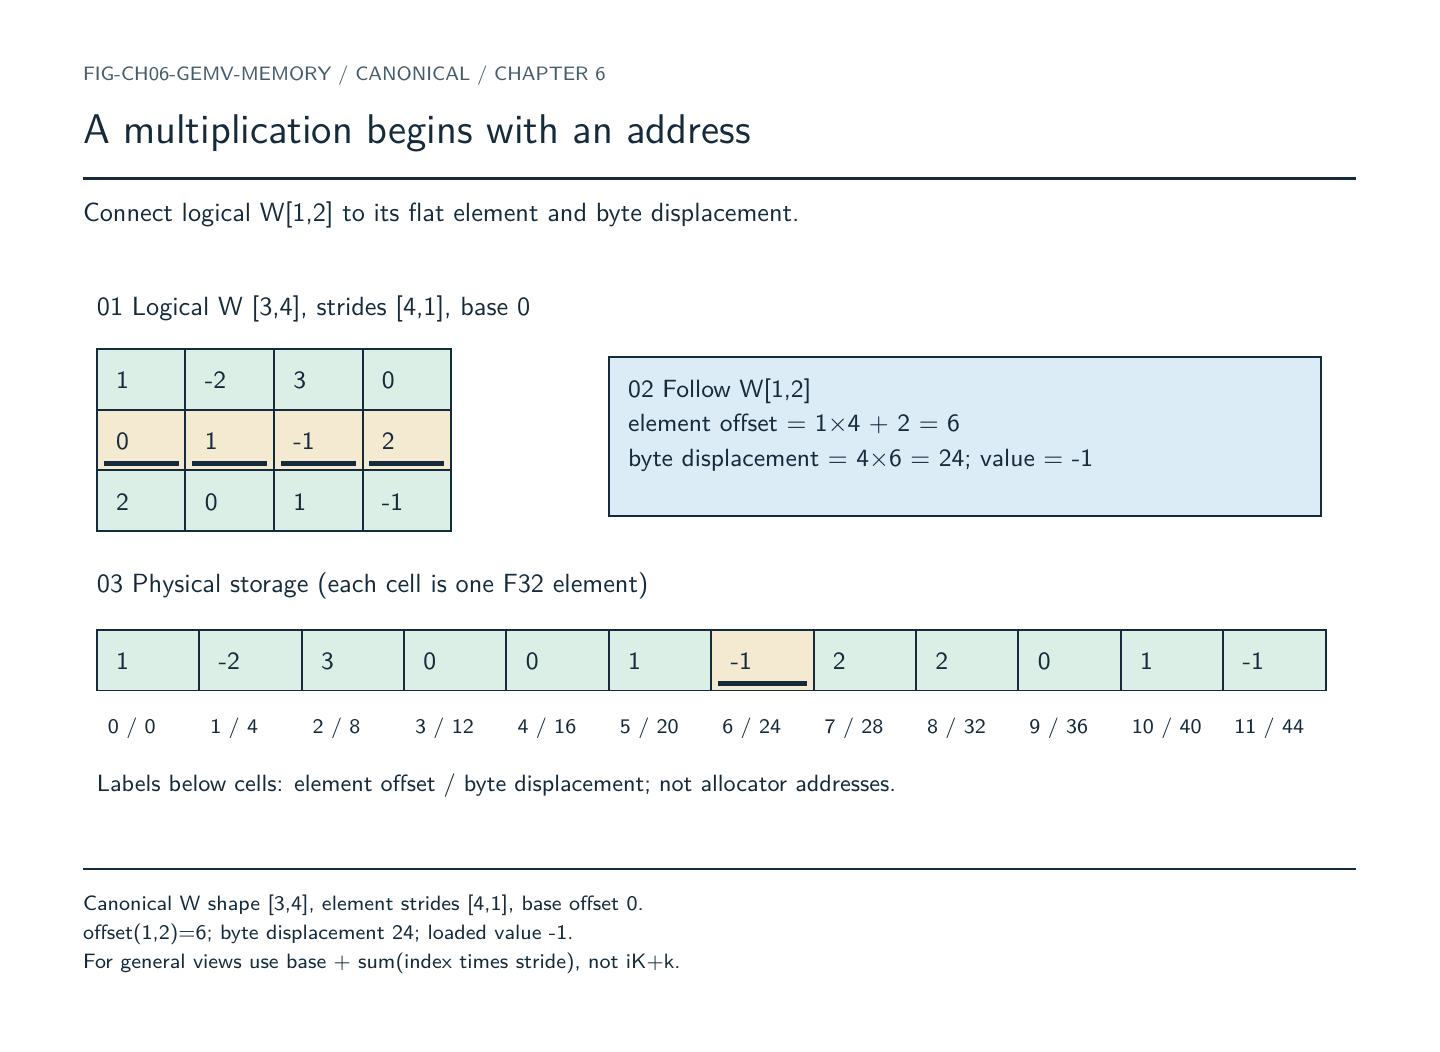
\begin{tikzpicture}[x=.5pt,y=-.5pt]
\path[use as bounding box] (0,0) rectangle (1000,720);
\path[fill=white,draw=none,line width=0.5pt] (0.0,0.0) rectangle (1000.0,720.0);
\node[inner sep=0pt,outer sep=0pt,anchor=base west,text={rgb,255:red,70;green,92;blue,107},font=\sffamily\fontsize{7.0}{8.4}\selectfont] at (40,38) {FIG-CH06-GEMV-MEMORY  /  CANONICAL / CHAPTER 6};
\node[inner sep=0pt,outer sep=0pt,anchor=base west,text={rgb,255:red,21;green,43;blue,60},font=\sffamily\fontsize{15.0}{18.0}\selectfont] at (40,84) {A multiplication begins with an address};
\draw[fill=none,draw={rgb,255:red,21;green,43;blue,60},line width=0.75pt] (40,109) -- (960,109);
\node[inner sep=0pt,outer sep=0pt,anchor=base west,text={rgb,255:red,21;green,43;blue,60},font=\sffamily\fontsize{9.5}{11.4}\selectfont] at (40,140) {Connect logical W[1,2] to its flat element and byte displacement.};
\node[inner sep=0pt,outer sep=0pt,anchor=base west,text={rgb,255:red,21;green,43;blue,60},font=\sffamily\fontsize{9.5}{11.4}\selectfont] at (50,208) {01  Logical W [3,4], strides [4,1], base 0};
\path[fill={rgb,255:red,220;green,239;blue,231},draw={rgb,255:red,21;green,43;blue,60},line width=0.7pt] (50.0,232.0) rectangle (114.0,276.0);
\node[inner sep=0pt,outer sep=0pt,anchor=base west,text={rgb,255:red,21;green,43;blue,60},font=\sffamily\fontsize{9.0}{10.799999999999999}\selectfont] at (64,261) {1};
\path[fill={rgb,255:red,220;green,239;blue,231},draw={rgb,255:red,21;green,43;blue,60},line width=0.7pt] (114.0,232.0) rectangle (178.0,276.0);
\node[inner sep=0pt,outer sep=0pt,anchor=base west,text={rgb,255:red,21;green,43;blue,60},font=\sffamily\fontsize{9.0}{10.799999999999999}\selectfont] at (128,261) {-2};
\path[fill={rgb,255:red,220;green,239;blue,231},draw={rgb,255:red,21;green,43;blue,60},line width=0.7pt] (178.0,232.0) rectangle (242.0,276.0);
\node[inner sep=0pt,outer sep=0pt,anchor=base west,text={rgb,255:red,21;green,43;blue,60},font=\sffamily\fontsize{9.0}{10.799999999999999}\selectfont] at (192,261) {3};
\path[fill={rgb,255:red,220;green,239;blue,231},draw={rgb,255:red,21;green,43;blue,60},line width=0.7pt] (242.0,232.0) rectangle (306.0,276.0);
\node[inner sep=0pt,outer sep=0pt,anchor=base west,text={rgb,255:red,21;green,43;blue,60},font=\sffamily\fontsize{9.0}{10.799999999999999}\selectfont] at (256,261) {0};
\path[fill={rgb,255:red,244;green,234;blue,210},draw={rgb,255:red,21;green,43;blue,60},line width=0.7pt] (50.0,276.0) rectangle (114.0,320.0);
\node[inner sep=0pt,outer sep=0pt,anchor=base west,text={rgb,255:red,21;green,43;blue,60},font=\sffamily\fontsize{9.0}{10.799999999999999}\selectfont] at (64,305) {0};
\draw[fill=none,draw={rgb,255:red,21;green,43;blue,60},line width=1.5pt] (55,315) -- (109,315);
\path[fill={rgb,255:red,244;green,234;blue,210},draw={rgb,255:red,21;green,43;blue,60},line width=0.7pt] (114.0,276.0) rectangle (178.0,320.0);
\node[inner sep=0pt,outer sep=0pt,anchor=base west,text={rgb,255:red,21;green,43;blue,60},font=\sffamily\fontsize{9.0}{10.799999999999999}\selectfont] at (128,305) {1};
\draw[fill=none,draw={rgb,255:red,21;green,43;blue,60},line width=1.5pt] (119,315) -- (173,315);
\path[fill={rgb,255:red,244;green,234;blue,210},draw={rgb,255:red,21;green,43;blue,60},line width=0.7pt] (178.0,276.0) rectangle (242.0,320.0);
\node[inner sep=0pt,outer sep=0pt,anchor=base west,text={rgb,255:red,21;green,43;blue,60},font=\sffamily\fontsize{9.0}{10.799999999999999}\selectfont] at (192,305) {-1};
\draw[fill=none,draw={rgb,255:red,21;green,43;blue,60},line width=1.5pt] (183,315) -- (237,315);
\path[fill={rgb,255:red,244;green,234;blue,210},draw={rgb,255:red,21;green,43;blue,60},line width=0.7pt] (242.0,276.0) rectangle (306.0,320.0);
\node[inner sep=0pt,outer sep=0pt,anchor=base west,text={rgb,255:red,21;green,43;blue,60},font=\sffamily\fontsize{9.0}{10.799999999999999}\selectfont] at (256,305) {2};
\draw[fill=none,draw={rgb,255:red,21;green,43;blue,60},line width=1.5pt] (247,315) -- (301,315);
\path[fill={rgb,255:red,220;green,239;blue,231},draw={rgb,255:red,21;green,43;blue,60},line width=0.7pt] (50.0,320.0) rectangle (114.0,364.0);
\node[inner sep=0pt,outer sep=0pt,anchor=base west,text={rgb,255:red,21;green,43;blue,60},font=\sffamily\fontsize{9.0}{10.799999999999999}\selectfont] at (64,349) {2};
\path[fill={rgb,255:red,220;green,239;blue,231},draw={rgb,255:red,21;green,43;blue,60},line width=0.7pt] (114.0,320.0) rectangle (178.0,364.0);
\node[inner sep=0pt,outer sep=0pt,anchor=base west,text={rgb,255:red,21;green,43;blue,60},font=\sffamily\fontsize{9.0}{10.799999999999999}\selectfont] at (128,349) {0};
\path[fill={rgb,255:red,220;green,239;blue,231},draw={rgb,255:red,21;green,43;blue,60},line width=0.7pt] (178.0,320.0) rectangle (242.0,364.0);
\node[inner sep=0pt,outer sep=0pt,anchor=base west,text={rgb,255:red,21;green,43;blue,60},font=\sffamily\fontsize{9.0}{10.799999999999999}\selectfont] at (192,349) {1};
\path[fill={rgb,255:red,220;green,239;blue,231},draw={rgb,255:red,21;green,43;blue,60},line width=0.7pt] (242.0,320.0) rectangle (306.0,364.0);
\node[inner sep=0pt,outer sep=0pt,anchor=base west,text={rgb,255:red,21;green,43;blue,60},font=\sffamily\fontsize{9.0}{10.799999999999999}\selectfont] at (256,349) {-1};
\path[fill={rgb,255:red,220;green,236;blue,247},draw={rgb,255:red,21;green,43;blue,60},line width=0.7pt] (420.0,238.0) rectangle (935.0,353.0);
\node[inner sep=0pt,outer sep=0pt,anchor=base west,text={rgb,255:red,21;green,43;blue,60},font=\sffamily\fontsize{9.0}{10.799999999999999}\selectfont] at (434,267) {02  Follow W[1,2]};
\node[inner sep=0pt,outer sep=0pt,anchor=base west,text={rgb,255:red,21;green,43;blue,60},font=\sffamily\fontsize{9.0}{10.799999999999999}\selectfont] at (434,292) {element offset = 1×4 + 2 = 6};
\node[inner sep=0pt,outer sep=0pt,anchor=base west,text={rgb,255:red,21;green,43;blue,60},font=\sffamily\fontsize{9.0}{10.799999999999999}\selectfont] at (434,317) {byte displacement = 4×6 = 24; value = -1};
\node[inner sep=0pt,outer sep=0pt,anchor=base west,text={rgb,255:red,21;green,43;blue,60},font=\sffamily\fontsize{9.5}{11.4}\selectfont] at (50,408) {03  Physical storage (each cell is one F32 element)};
\path[fill={rgb,255:red,220;green,239;blue,231},draw={rgb,255:red,21;green,43;blue,60},line width=0.7pt] (50.0,435.0) rectangle (124.0,479.0);
\node[inner sep=0pt,outer sep=0pt,anchor=base west,text={rgb,255:red,21;green,43;blue,60},font=\sffamily\fontsize{9.0}{10.799999999999999}\selectfont] at (64,464) {1};
\path[fill={rgb,255:red,220;green,239;blue,231},draw={rgb,255:red,21;green,43;blue,60},line width=0.7pt] (124.0,435.0) rectangle (198.0,479.0);
\node[inner sep=0pt,outer sep=0pt,anchor=base west,text={rgb,255:red,21;green,43;blue,60},font=\sffamily\fontsize{9.0}{10.799999999999999}\selectfont] at (138,464) {-2};
\path[fill={rgb,255:red,220;green,239;blue,231},draw={rgb,255:red,21;green,43;blue,60},line width=0.7pt] (198.0,435.0) rectangle (272.0,479.0);
\node[inner sep=0pt,outer sep=0pt,anchor=base west,text={rgb,255:red,21;green,43;blue,60},font=\sffamily\fontsize{9.0}{10.799999999999999}\selectfont] at (212,464) {3};
\path[fill={rgb,255:red,220;green,239;blue,231},draw={rgb,255:red,21;green,43;blue,60},line width=0.7pt] (272.0,435.0) rectangle (346.0,479.0);
\node[inner sep=0pt,outer sep=0pt,anchor=base west,text={rgb,255:red,21;green,43;blue,60},font=\sffamily\fontsize{9.0}{10.799999999999999}\selectfont] at (286,464) {0};
\path[fill={rgb,255:red,220;green,239;blue,231},draw={rgb,255:red,21;green,43;blue,60},line width=0.7pt] (346.0,435.0) rectangle (420.0,479.0);
\node[inner sep=0pt,outer sep=0pt,anchor=base west,text={rgb,255:red,21;green,43;blue,60},font=\sffamily\fontsize{9.0}{10.799999999999999}\selectfont] at (360,464) {0};
\path[fill={rgb,255:red,220;green,239;blue,231},draw={rgb,255:red,21;green,43;blue,60},line width=0.7pt] (420.0,435.0) rectangle (494.0,479.0);
\node[inner sep=0pt,outer sep=0pt,anchor=base west,text={rgb,255:red,21;green,43;blue,60},font=\sffamily\fontsize{9.0}{10.799999999999999}\selectfont] at (434,464) {1};
\path[fill={rgb,255:red,244;green,234;blue,210},draw={rgb,255:red,21;green,43;blue,60},line width=0.7pt] (494.0,435.0) rectangle (568.0,479.0);
\node[inner sep=0pt,outer sep=0pt,anchor=base west,text={rgb,255:red,21;green,43;blue,60},font=\sffamily\fontsize{9.0}{10.799999999999999}\selectfont] at (508,464) {-1};
\draw[fill=none,draw={rgb,255:red,21;green,43;blue,60},line width=1.5pt] (499,474) -- (563,474);
\path[fill={rgb,255:red,220;green,239;blue,231},draw={rgb,255:red,21;green,43;blue,60},line width=0.7pt] (568.0,435.0) rectangle (642.0,479.0);
\node[inner sep=0pt,outer sep=0pt,anchor=base west,text={rgb,255:red,21;green,43;blue,60},font=\sffamily\fontsize{9.0}{10.799999999999999}\selectfont] at (582,464) {2};
\path[fill={rgb,255:red,220;green,239;blue,231},draw={rgb,255:red,21;green,43;blue,60},line width=0.7pt] (642.0,435.0) rectangle (716.0,479.0);
\node[inner sep=0pt,outer sep=0pt,anchor=base west,text={rgb,255:red,21;green,43;blue,60},font=\sffamily\fontsize{9.0}{10.799999999999999}\selectfont] at (656,464) {2};
\path[fill={rgb,255:red,220;green,239;blue,231},draw={rgb,255:red,21;green,43;blue,60},line width=0.7pt] (716.0,435.0) rectangle (790.0,479.0);
\node[inner sep=0pt,outer sep=0pt,anchor=base west,text={rgb,255:red,21;green,43;blue,60},font=\sffamily\fontsize{9.0}{10.799999999999999}\selectfont] at (730,464) {0};
\path[fill={rgb,255:red,220;green,239;blue,231},draw={rgb,255:red,21;green,43;blue,60},line width=0.7pt] (790.0,435.0) rectangle (864.0,479.0);
\node[inner sep=0pt,outer sep=0pt,anchor=base west,text={rgb,255:red,21;green,43;blue,60},font=\sffamily\fontsize{9.0}{10.799999999999999}\selectfont] at (804,464) {1};
\path[fill={rgb,255:red,220;green,239;blue,231},draw={rgb,255:red,21;green,43;blue,60},line width=0.7pt] (864.0,435.0) rectangle (938.0,479.0);
\node[inner sep=0pt,outer sep=0pt,anchor=base west,text={rgb,255:red,21;green,43;blue,60},font=\sffamily\fontsize{9.0}{10.799999999999999}\selectfont] at (878,464) {-1};
\node[inner sep=0pt,outer sep=0pt,anchor=base west,text={rgb,255:red,21;green,43;blue,60},font=\sffamily\fontsize{7.5}{9.0}\selectfont] at (58,510) {0 / 0};
\node[inner sep=0pt,outer sep=0pt,anchor=base west,text={rgb,255:red,21;green,43;blue,60},font=\sffamily\fontsize{7.5}{9.0}\selectfont] at (132,510) {1 / 4};
\node[inner sep=0pt,outer sep=0pt,anchor=base west,text={rgb,255:red,21;green,43;blue,60},font=\sffamily\fontsize{7.5}{9.0}\selectfont] at (206,510) {2 / 8};
\node[inner sep=0pt,outer sep=0pt,anchor=base west,text={rgb,255:red,21;green,43;blue,60},font=\sffamily\fontsize{7.5}{9.0}\selectfont] at (280,510) {3 / 12};
\node[inner sep=0pt,outer sep=0pt,anchor=base west,text={rgb,255:red,21;green,43;blue,60},font=\sffamily\fontsize{7.5}{9.0}\selectfont] at (354,510) {4 / 16};
\node[inner sep=0pt,outer sep=0pt,anchor=base west,text={rgb,255:red,21;green,43;blue,60},font=\sffamily\fontsize{7.5}{9.0}\selectfont] at (428,510) {5 / 20};
\node[inner sep=0pt,outer sep=0pt,anchor=base west,text={rgb,255:red,21;green,43;blue,60},font=\sffamily\fontsize{7.5}{9.0}\selectfont] at (502,510) {6 / 24};
\node[inner sep=0pt,outer sep=0pt,anchor=base west,text={rgb,255:red,21;green,43;blue,60},font=\sffamily\fontsize{7.5}{9.0}\selectfont] at (576,510) {7 / 28};
\node[inner sep=0pt,outer sep=0pt,anchor=base west,text={rgb,255:red,21;green,43;blue,60},font=\sffamily\fontsize{7.5}{9.0}\selectfont] at (650,510) {8 / 32};
\node[inner sep=0pt,outer sep=0pt,anchor=base west,text={rgb,255:red,21;green,43;blue,60},font=\sffamily\fontsize{7.5}{9.0}\selectfont] at (724,510) {9 / 36};
\node[inner sep=0pt,outer sep=0pt,anchor=base west,text={rgb,255:red,21;green,43;blue,60},font=\sffamily\fontsize{7.5}{9.0}\selectfont] at (798,510) {10 / 40};
\node[inner sep=0pt,outer sep=0pt,anchor=base west,text={rgb,255:red,21;green,43;blue,60},font=\sffamily\fontsize{7.5}{9.0}\selectfont] at (872,510) {11 / 44};
\node[inner sep=0pt,outer sep=0pt,anchor=base west,text={rgb,255:red,21;green,43;blue,60},font=\sffamily\fontsize{8.5}{10.2}\selectfont] at (50,552) {Labels below cells: element offset / byte displacement; not allocator addresses.};
\draw[fill=none,draw={rgb,255:red,21;green,43;blue,60},line width=0.75pt] (40,608) -- (960,608);
\node[inner sep=0pt,outer sep=0pt,anchor=base west,text={rgb,255:red,21;green,43;blue,60},font=\sffamily\fontsize{7.5}{9.0}\selectfont] at (40,638) {Canonical W shape [3,4], element strides [4,1], base offset 0.};
\node[inner sep=0pt,outer sep=0pt,anchor=base west,text={rgb,255:red,21;green,43;blue,60},font=\sffamily\fontsize{7.5}{9.0}\selectfont] at (40,659) {offset(1,2)=6; byte displacement 24; loaded value -1.};
\node[inner sep=0pt,outer sep=0pt,anchor=base west,text={rgb,255:red,21;green,43;blue,60},font=\sffamily\fontsize{7.5}{9.0}\selectfont] at (40,680) {For general views use base + sum(index times stride), not iK+k.};
\end{tikzpicture}
}\caption{Logical W maps to twelve F32 storage cells; index one comma two is offset six and byte twenty-four.}\end{figure}

The reference calls checked view access; it does not replace that
mapping with \texttt{i*K+k} for arbitrary inputs. A transposed view
changes strides without moving values. A zero-stride immutable view may
reuse one storage cell at several logical positions. Both can be valid
reference operands. The blocked kernel later requires canonical
row-major slices so its simplified arithmetic is justified by an
explicit boundary check, not by an assumption hidden in a loop.

The canonical
\href{https://github.com/hermonai/inside-the-llm-engine/blob/astra-visual-rewrite/code/reference/fixtures/chapter06-visual.json}{fixture}
stores inputs only. The independent
\href{https://github.com/hermonai/inside-the-llm-engine/blob/astra-visual-rewrite/code/reference/python/chapter06_visual_oracle.py}{Python
visual oracle} derives outputs, addresses, contribution traces, and tile
ranges. The
\href{https://github.com/hermonai/inside-the-llm-engine/blob/astra-visual-rewrite/code/mini-engine/crates/engine0/examples/chapter06_visual_trace.rs}{Rust
visual example} uses the real tensor and linear APIs. A parity script
compares the results; neither a manually typed answer nor the artwork
alone is the specification.

\subsection{Matrix times matrix}\label{matrix-times-matrix}

Let \(\mathbf{A}\in\mathbb{R}^{M\times K}\) and
\(\mathbf{B}\in\mathbb{R}^{K\times N}\). Their matrix product
\(\mathbf{C}=\mathbf{A}\mathbf{B}\in\mathbb{R}^{M\times N}\) has
elements

\[
C_{ij}=\sum_{k=0}^{K-1}A_{ik}B_{kj},
\qquad 0\le i<M,\quad 0\le j<N.
\]

Every output cell is the dot product of row \(i\) from \(A\) and column
\(j\) from \(B\). The inner dimensions must agree. There is no
requirement that \(M\), \(K\), and \(N\) equal one another.

The two matrices are independent inputs to one contraction. An arrow
from \(A\) into \(B\) would incorrectly suggest that the first produces
the second.

See the canonical
\href{https://github.com/hermonai/inside-the-llm-engine/blob/astra-visual-rewrite/diagrams/linear/gemm-shape-contract.txt}{GEMM
shape contract} and
\href{https://github.com/hermonai/inside-the-llm-engine/blob/astra-visual-rewrite/diagrams/linear/gemm-one-output-cell.txt}{one-output-cell
diagram}. The common acronym \textbf{GEMM} comes from the BLAS general
matrix-matrix family; \textbf{GEMV} names the corresponding
matrix-vector family. ENGINE-2 implements a much smaller contract than
full BLAS: no transpose flags, scaling parameters, mixed layouts, or
in-place accumulation into caller storage.

\subsection{Shape contracts are execution
contracts}\label{shape-contracts-are-execution-contracts}

The symbols \(M\), \(K\), and \(N\) are not decorative labels. They
control loop bounds, allocation size, and address arithmetic. Each
dimension has a role:

\begin{itemize}
\tightlist
\item
  \(M\) counts independent rows of the left operand and output;
\item
  \(K\) counts contributions reduced into each output value;
\item
  \(N\) counts columns of the right operand and output.
\end{itemize}

The agreement rule is positional. For \(A:[M,K]\) and \(B:[K,N]\), the
last axis of \(A\) equals the first axis of \(B\). Equal total element
counts are irrelevant. Shapes \texttt{{[}2,6{]}} and \texttt{{[}3,4{]}}
both contain twelve values, but they cannot occupy the two sides of this
product because 6 does not equal 3. Reshaping one operand would change
the mathematical problem and must be an explicit caller action.

The dimension roles also explain orientation. ENGINE-1 stores projection
weights as \texttt{{[}vocabulary,\ hidden{]}}. Vocabulary candidates are
output rows, so \(M=V\) and \(K=D\). Multiplying by hidden
\texttt{{[}D{]}} naturally returns \texttt{{[}V{]}}. If the weights were
stored \texttt{{[}D,V{]}}, the call would require a transpose view or a
different contract. A kernel must never guess orientation from equal
numbers.

Shape validation precedes output allocation for two reasons. First, it
avoids spending memory on a computation that has no defined result.
Second, it keeps failure deterministic: an inner-dimension mismatch
remains that typed error rather than sometimes becoming allocation
failure first. Output element count \(MN\) is checked independently
because valid input views with empty K can still describe an
unrepresentably large prospective output.

Ranks are checked before individual axes are read.
\texttt{gemv\_reference} cannot interpret a rank-2 shape as a vector
merely because it contains one column;
\texttt{\seqsplit{matmul\_reference}} cannot flatten a higher-rank
tensor. Later engines will define batching explicitly. Treating extra
axes as implicit batches here would create a second, undocumented
operator.

This strictness makes error messages part of the kernel API.
\texttt{RankMismatch} names the operation and operand.
\texttt{\seqsplit{InnerDimensionMismatch}} reports both K values.
\texttt{\seqsplit{OutputShapeOverflow}} reports M and N. Callers can
diagnose which contract failed without reconstructing it from a generic
bounds error.

\subsection{One output cell by hand}\label{one-output-cell-by-hand}

Keep \(A=W\) from GEMV, and place two input vectors into the columns of
\(B\):

\[
B=
\begin{bmatrix}
2&1\\
1&-1\\
-1&2\\
0.5&0
\end{bmatrix}.
\]

The selected output cell follows row 0 and column 1, matching the same
\(k\):

\[
C_{01}=1(1)+(-2)(-1)+3(2)+0(0)=9.
\]

Therefore

\[
C=
\begin{bmatrix}
-3&9\\
3&-3\\
2.5&4
\end{bmatrix}.
\]

\begin{figure}[H]\centering\resizebox{\linewidth}{!}{% Generated from figures/generated/ch06-gemm.svg; do not hand edit.
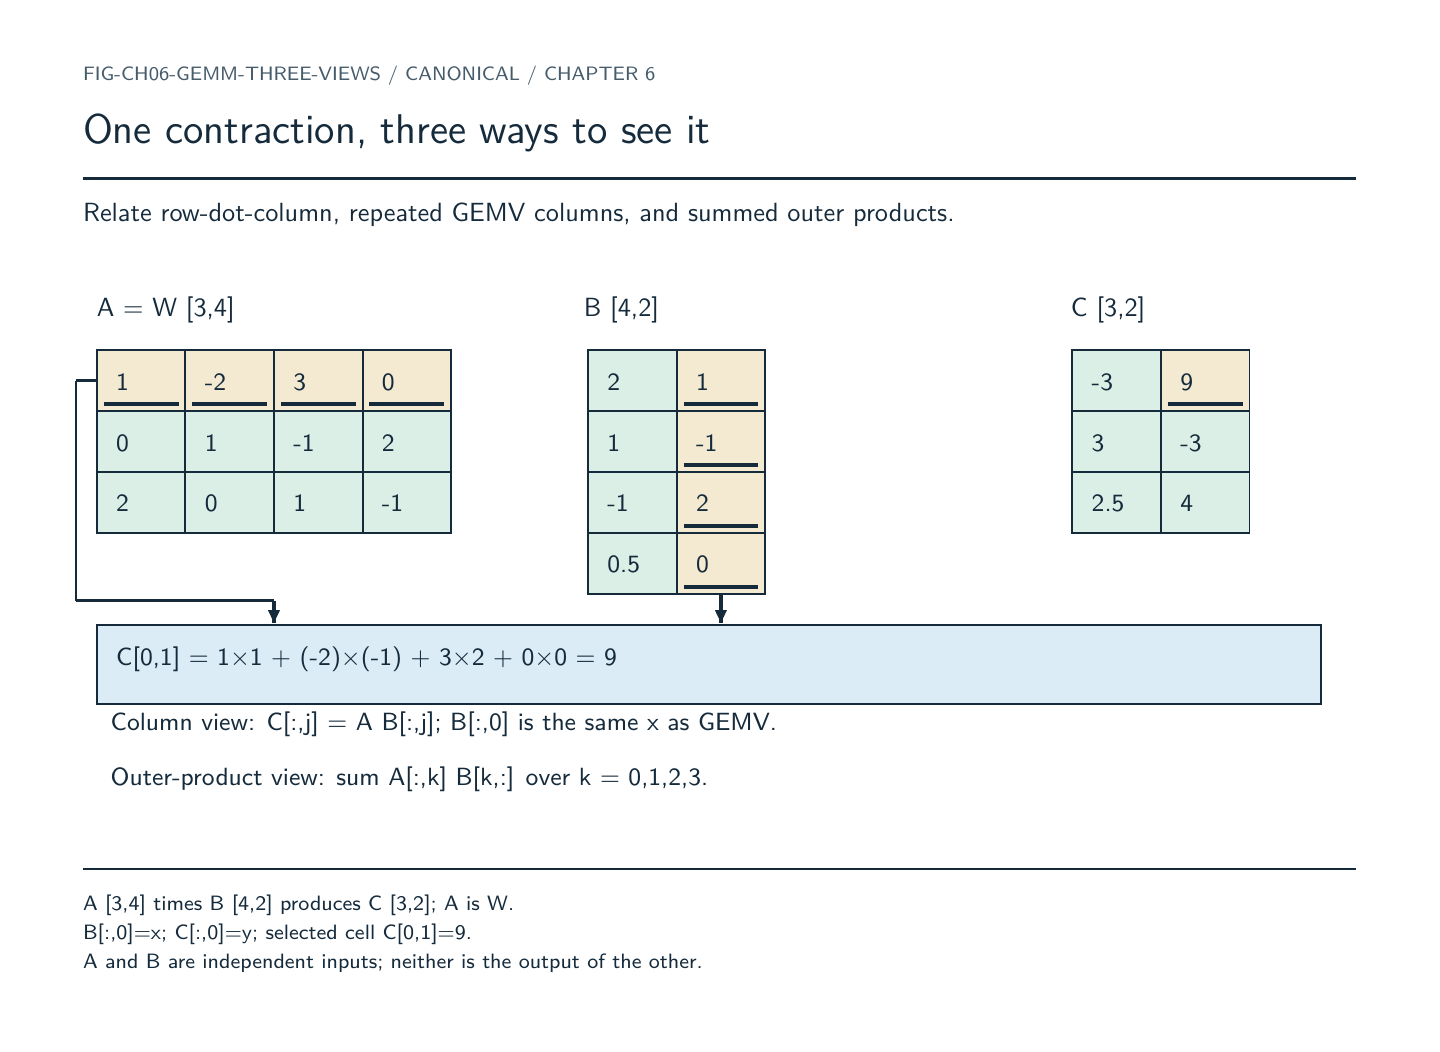
\begin{tikzpicture}[x=.5pt,y=-.5pt]
\path[use as bounding box] (0,0) rectangle (1000,720);
\path[fill=white,draw=none,line width=0.5pt] (0.0,0.0) rectangle (1000.0,720.0);
\node[inner sep=0pt,outer sep=0pt,anchor=base west,text={rgb,255:red,70;green,92;blue,107},font=\sffamily\fontsize{7.0}{8.4}\selectfont] at (40,38) {FIG-CH06-GEMM-THREE-VIEWS  /  CANONICAL / CHAPTER 6};
\node[inner sep=0pt,outer sep=0pt,anchor=base west,text={rgb,255:red,21;green,43;blue,60},font=\sffamily\fontsize{15.0}{18.0}\selectfont] at (40,84) {One contraction, three ways to see it};
\draw[fill=none,draw={rgb,255:red,21;green,43;blue,60},line width=0.75pt] (40,109) -- (960,109);
\node[inner sep=0pt,outer sep=0pt,anchor=base west,text={rgb,255:red,21;green,43;blue,60},font=\sffamily\fontsize{9.5}{11.4}\selectfont] at (40,140) {Relate row-dot-column, repeated GEMV columns, and summed outer products.};
\node[inner sep=0pt,outer sep=0pt,anchor=base west,text={rgb,255:red,21;green,43;blue,60},font=\sffamily\fontsize{9.5}{11.4}\selectfont] at (50,209) {A = W [3,4]};
\path[fill={rgb,255:red,244;green,234;blue,210},draw={rgb,255:red,21;green,43;blue,60},line width=0.7pt] (50.0,233.0) rectangle (114.0,277.0);
\node[inner sep=0pt,outer sep=0pt,anchor=base west,text={rgb,255:red,21;green,43;blue,60},font=\sffamily\fontsize{9.0}{10.799999999999999}\selectfont] at (64,262) {1};
\draw[fill=none,draw={rgb,255:red,21;green,43;blue,60},line width=1.5pt] (55,272) -- (109,272);
\path[fill={rgb,255:red,244;green,234;blue,210},draw={rgb,255:red,21;green,43;blue,60},line width=0.7pt] (114.0,233.0) rectangle (178.0,277.0);
\node[inner sep=0pt,outer sep=0pt,anchor=base west,text={rgb,255:red,21;green,43;blue,60},font=\sffamily\fontsize{9.0}{10.799999999999999}\selectfont] at (128,262) {-2};
\draw[fill=none,draw={rgb,255:red,21;green,43;blue,60},line width=1.5pt] (119,272) -- (173,272);
\path[fill={rgb,255:red,244;green,234;blue,210},draw={rgb,255:red,21;green,43;blue,60},line width=0.7pt] (178.0,233.0) rectangle (242.0,277.0);
\node[inner sep=0pt,outer sep=0pt,anchor=base west,text={rgb,255:red,21;green,43;blue,60},font=\sffamily\fontsize{9.0}{10.799999999999999}\selectfont] at (192,262) {3};
\draw[fill=none,draw={rgb,255:red,21;green,43;blue,60},line width=1.5pt] (183,272) -- (237,272);
\path[fill={rgb,255:red,244;green,234;blue,210},draw={rgb,255:red,21;green,43;blue,60},line width=0.7pt] (242.0,233.0) rectangle (306.0,277.0);
\node[inner sep=0pt,outer sep=0pt,anchor=base west,text={rgb,255:red,21;green,43;blue,60},font=\sffamily\fontsize{9.0}{10.799999999999999}\selectfont] at (256,262) {0};
\draw[fill=none,draw={rgb,255:red,21;green,43;blue,60},line width=1.5pt] (247,272) -- (301,272);
\path[fill={rgb,255:red,220;green,239;blue,231},draw={rgb,255:red,21;green,43;blue,60},line width=0.7pt] (50.0,277.0) rectangle (114.0,321.0);
\node[inner sep=0pt,outer sep=0pt,anchor=base west,text={rgb,255:red,21;green,43;blue,60},font=\sffamily\fontsize{9.0}{10.799999999999999}\selectfont] at (64,306) {0};
\path[fill={rgb,255:red,220;green,239;blue,231},draw={rgb,255:red,21;green,43;blue,60},line width=0.7pt] (114.0,277.0) rectangle (178.0,321.0);
\node[inner sep=0pt,outer sep=0pt,anchor=base west,text={rgb,255:red,21;green,43;blue,60},font=\sffamily\fontsize{9.0}{10.799999999999999}\selectfont] at (128,306) {1};
\path[fill={rgb,255:red,220;green,239;blue,231},draw={rgb,255:red,21;green,43;blue,60},line width=0.7pt] (178.0,277.0) rectangle (242.0,321.0);
\node[inner sep=0pt,outer sep=0pt,anchor=base west,text={rgb,255:red,21;green,43;blue,60},font=\sffamily\fontsize{9.0}{10.799999999999999}\selectfont] at (192,306) {-1};
\path[fill={rgb,255:red,220;green,239;blue,231},draw={rgb,255:red,21;green,43;blue,60},line width=0.7pt] (242.0,277.0) rectangle (306.0,321.0);
\node[inner sep=0pt,outer sep=0pt,anchor=base west,text={rgb,255:red,21;green,43;blue,60},font=\sffamily\fontsize{9.0}{10.799999999999999}\selectfont] at (256,306) {2};
\path[fill={rgb,255:red,220;green,239;blue,231},draw={rgb,255:red,21;green,43;blue,60},line width=0.7pt] (50.0,321.0) rectangle (114.0,365.0);
\node[inner sep=0pt,outer sep=0pt,anchor=base west,text={rgb,255:red,21;green,43;blue,60},font=\sffamily\fontsize{9.0}{10.799999999999999}\selectfont] at (64,350) {2};
\path[fill={rgb,255:red,220;green,239;blue,231},draw={rgb,255:red,21;green,43;blue,60},line width=0.7pt] (114.0,321.0) rectangle (178.0,365.0);
\node[inner sep=0pt,outer sep=0pt,anchor=base west,text={rgb,255:red,21;green,43;blue,60},font=\sffamily\fontsize{9.0}{10.799999999999999}\selectfont] at (128,350) {0};
\path[fill={rgb,255:red,220;green,239;blue,231},draw={rgb,255:red,21;green,43;blue,60},line width=0.7pt] (178.0,321.0) rectangle (242.0,365.0);
\node[inner sep=0pt,outer sep=0pt,anchor=base west,text={rgb,255:red,21;green,43;blue,60},font=\sffamily\fontsize{9.0}{10.799999999999999}\selectfont] at (192,350) {1};
\path[fill={rgb,255:red,220;green,239;blue,231},draw={rgb,255:red,21;green,43;blue,60},line width=0.7pt] (242.0,321.0) rectangle (306.0,365.0);
\node[inner sep=0pt,outer sep=0pt,anchor=base west,text={rgb,255:red,21;green,43;blue,60},font=\sffamily\fontsize{9.0}{10.799999999999999}\selectfont] at (256,350) {-1};
\node[inner sep=0pt,outer sep=0pt,anchor=base west,text={rgb,255:red,21;green,43;blue,60},font=\sffamily\fontsize{9.5}{11.4}\selectfont] at (402,209) {B [4,2]};
\path[fill={rgb,255:red,220;green,239;blue,231},draw={rgb,255:red,21;green,43;blue,60},line width=0.7pt] (405.0,233.0) rectangle (469.0,277.0);
\node[inner sep=0pt,outer sep=0pt,anchor=base west,text={rgb,255:red,21;green,43;blue,60},font=\sffamily\fontsize{9.0}{10.799999999999999}\selectfont] at (419,262) {2};
\path[fill={rgb,255:red,244;green,234;blue,210},draw={rgb,255:red,21;green,43;blue,60},line width=0.7pt] (469.0,233.0) rectangle (533.0,277.0);
\node[inner sep=0pt,outer sep=0pt,anchor=base west,text={rgb,255:red,21;green,43;blue,60},font=\sffamily\fontsize{9.0}{10.799999999999999}\selectfont] at (483,262) {1};
\draw[fill=none,draw={rgb,255:red,21;green,43;blue,60},line width=1.5pt] (474,272) -- (528,272);
\path[fill={rgb,255:red,220;green,239;blue,231},draw={rgb,255:red,21;green,43;blue,60},line width=0.7pt] (405.0,277.0) rectangle (469.0,321.0);
\node[inner sep=0pt,outer sep=0pt,anchor=base west,text={rgb,255:red,21;green,43;blue,60},font=\sffamily\fontsize{9.0}{10.799999999999999}\selectfont] at (419,306) {1};
\path[fill={rgb,255:red,244;green,234;blue,210},draw={rgb,255:red,21;green,43;blue,60},line width=0.7pt] (469.0,277.0) rectangle (533.0,321.0);
\node[inner sep=0pt,outer sep=0pt,anchor=base west,text={rgb,255:red,21;green,43;blue,60},font=\sffamily\fontsize{9.0}{10.799999999999999}\selectfont] at (483,306) {-1};
\draw[fill=none,draw={rgb,255:red,21;green,43;blue,60},line width=1.5pt] (474,316) -- (528,316);
\path[fill={rgb,255:red,220;green,239;blue,231},draw={rgb,255:red,21;green,43;blue,60},line width=0.7pt] (405.0,321.0) rectangle (469.0,365.0);
\node[inner sep=0pt,outer sep=0pt,anchor=base west,text={rgb,255:red,21;green,43;blue,60},font=\sffamily\fontsize{9.0}{10.799999999999999}\selectfont] at (419,350) {-1};
\path[fill={rgb,255:red,244;green,234;blue,210},draw={rgb,255:red,21;green,43;blue,60},line width=0.7pt] (469.0,321.0) rectangle (533.0,365.0);
\node[inner sep=0pt,outer sep=0pt,anchor=base west,text={rgb,255:red,21;green,43;blue,60},font=\sffamily\fontsize{9.0}{10.799999999999999}\selectfont] at (483,350) {2};
\draw[fill=none,draw={rgb,255:red,21;green,43;blue,60},line width=1.5pt] (474,360) -- (528,360);
\path[fill={rgb,255:red,220;green,239;blue,231},draw={rgb,255:red,21;green,43;blue,60},line width=0.7pt] (405.0,365.0) rectangle (469.0,409.0);
\node[inner sep=0pt,outer sep=0pt,anchor=base west,text={rgb,255:red,21;green,43;blue,60},font=\sffamily\fontsize{9.0}{10.799999999999999}\selectfont] at (419,394) {0.5};
\path[fill={rgb,255:red,244;green,234;blue,210},draw={rgb,255:red,21;green,43;blue,60},line width=0.7pt] (469.0,365.0) rectangle (533.0,409.0);
\node[inner sep=0pt,outer sep=0pt,anchor=base west,text={rgb,255:red,21;green,43;blue,60},font=\sffamily\fontsize{9.0}{10.799999999999999}\selectfont] at (483,394) {0};
\draw[fill=none,draw={rgb,255:red,21;green,43;blue,60},line width=1.5pt] (474,404) -- (528,404);
\node[inner sep=0pt,outer sep=0pt,anchor=base west,text={rgb,255:red,21;green,43;blue,60},font=\sffamily\fontsize{9.5}{11.4}\selectfont] at (754,209) {C [3,2]};
\path[fill={rgb,255:red,220;green,239;blue,231},draw={rgb,255:red,21;green,43;blue,60},line width=0.7pt] (755.0,233.0) rectangle (819.0,277.0);
\node[inner sep=0pt,outer sep=0pt,anchor=base west,text={rgb,255:red,21;green,43;blue,60},font=\sffamily\fontsize{9.0}{10.799999999999999}\selectfont] at (769,262) {-3};
\path[fill={rgb,255:red,244;green,234;blue,210},draw={rgb,255:red,21;green,43;blue,60},line width=0.7pt] (819.0,233.0) rectangle (883.0,277.0);
\node[inner sep=0pt,outer sep=0pt,anchor=base west,text={rgb,255:red,21;green,43;blue,60},font=\sffamily\fontsize{9.0}{10.799999999999999}\selectfont] at (833,262) {9};
\draw[fill=none,draw={rgb,255:red,21;green,43;blue,60},line width=1.5pt] (824,272) -- (878,272);
\path[fill={rgb,255:red,220;green,239;blue,231},draw={rgb,255:red,21;green,43;blue,60},line width=0.7pt] (755.0,277.0) rectangle (819.0,321.0);
\node[inner sep=0pt,outer sep=0pt,anchor=base west,text={rgb,255:red,21;green,43;blue,60},font=\sffamily\fontsize{9.0}{10.799999999999999}\selectfont] at (769,306) {3};
\path[fill={rgb,255:red,220;green,239;blue,231},draw={rgb,255:red,21;green,43;blue,60},line width=0.7pt] (819.0,277.0) rectangle (883.0,321.0);
\node[inner sep=0pt,outer sep=0pt,anchor=base west,text={rgb,255:red,21;green,43;blue,60},font=\sffamily\fontsize{9.0}{10.799999999999999}\selectfont] at (833,306) {-3};
\path[fill={rgb,255:red,220;green,239;blue,231},draw={rgb,255:red,21;green,43;blue,60},line width=0.7pt] (755.0,321.0) rectangle (819.0,365.0);
\node[inner sep=0pt,outer sep=0pt,anchor=base west,text={rgb,255:red,21;green,43;blue,60},font=\sffamily\fontsize{9.0}{10.799999999999999}\selectfont] at (769,350) {2.5};
\path[fill={rgb,255:red,220;green,239;blue,231},draw={rgb,255:red,21;green,43;blue,60},line width=0.7pt] (819.0,321.0) rectangle (883.0,365.0);
\node[inner sep=0pt,outer sep=0pt,anchor=base west,text={rgb,255:red,21;green,43;blue,60},font=\sffamily\fontsize{9.0}{10.799999999999999}\selectfont] at (833,350) {4};
\draw[fill=none,draw={rgb,255:red,21;green,43;blue,60},line width=0.75pt] (50,255) -- (35,255);
\draw[fill=none,draw={rgb,255:red,21;green,43;blue,60},line width=0.75pt] (35,255) -- (35,414);
\draw[fill=none,draw={rgb,255:red,21;green,43;blue,60},line width=0.75pt] (35,414) -- (178,414);
\draw[fill=none,draw={rgb,255:red,21;green,43;blue,60},line width=1.25pt] (178,414) -- (178,430);
\path[fill={rgb,255:red,21;green,43;blue,60},draw=none,line width=0.5pt] (178.00,430.00) -- (173.65,421.00) -- (182.35,421.00) -- cycle;
\draw[fill=none,draw={rgb,255:red,21;green,43;blue,60},line width=1.25pt] (501,410) -- (501,430);
\path[fill={rgb,255:red,21;green,43;blue,60},draw=none,line width=0.5pt] (501.00,430.00) -- (496.65,421.00) -- (505.35,421.00) -- cycle;
\path[fill={rgb,255:red,220;green,236;blue,247},draw={rgb,255:red,21;green,43;blue,60},line width=0.7pt] (50.0,432.0) rectangle (935.0,489.0);
\node[inner sep=0pt,outer sep=0pt,anchor=base west,text={rgb,255:red,21;green,43;blue,60},font=\sffamily\fontsize{9.0}{10.799999999999999}\selectfont] at (64,461) {C[0,1] = 1×1 + (-2)×(-1) + 3×2 + 0×0 = 9};
\node[inner sep=0pt,outer sep=0pt,anchor=base west,text={rgb,255:red,21;green,43;blue,60},font=\sffamily\fontsize{9.0}{10.799999999999999}\selectfont] at (64,486) {};
\node[inner sep=0pt,outer sep=0pt,anchor=base west,text={rgb,255:red,21;green,43;blue,60},font=\sffamily\fontsize{9.0}{10.799999999999999}\selectfont] at (60,508) {Column view: C[:,j] = A B[:,j]; B[:,0] is the same x as GEMV.};
\node[inner sep=0pt,outer sep=0pt,anchor=base west,text={rgb,255:red,21;green,43;blue,60},font=\sffamily\fontsize{9.0}{10.799999999999999}\selectfont] at (60,548) {Outer-product view: sum A[:,k] B[k,:] over k = 0,1,2,3.};
\draw[fill=none,draw={rgb,255:red,21;green,43;blue,60},line width=0.75pt] (40,608) -- (960,608);
\node[inner sep=0pt,outer sep=0pt,anchor=base west,text={rgb,255:red,21;green,43;blue,60},font=\sffamily\fontsize{7.5}{9.0}\selectfont] at (40,638) {A [3,4] times B [4,2] produces C [3,2]; A is W.};
\node[inner sep=0pt,outer sep=0pt,anchor=base west,text={rgb,255:red,21;green,43;blue,60},font=\sffamily\fontsize{7.5}{9.0}\selectfont] at (40,659) {B[:,0]=x; C[:,0]=y; selected cell C[0,1]=9.};
\node[inner sep=0pt,outer sep=0pt,anchor=base west,text={rgb,255:red,21;green,43;blue,60},font=\sffamily\fontsize{7.5}{9.0}\selectfont] at (40,680) {A and B are independent inputs; neither is the output of the other.};
\end{tikzpicture}
}\caption{Selected row and column independently feed the dot product for C zero comma one, with column and outer-product interpretations.}\end{figure}

The same contraction has two other useful interpretations. First, each
column of \(B\) is a GEMV input:

\[
C_{:,j}=A B_{:,j},\qquad B_{:,0}=\mathbf{x},\qquad C_{:,0}=\mathbf{y}.
\]

Second, one reduction index contributes a whole rank-one matrix:

\[
C=\sum_{k=0}^{K-1} A_{:,k}B_{k,:}.
\]

Here \(A_{:,k}\) is a column of length \(M\) and \(B_{k,:}\) a row of
length \(N\); their outer product has shape \texttt{{[}M,N{]}}. For
\(k=0\), the contribution is \([1,0,2]^{\mathsf T}[2,1]\), giving rows
\texttt{{[}2,1{]}}, \texttt{{[}0,0{]}}, \texttt{{[}4,2{]}}. Adding all
four outer products yields the same \(C\). Row-dot-column explains a
cell, repeated GEMV explains columns, and outer products explain reuse
across cells. None changes the mathematical result over real numbers.

Tracing all six cells matters. A test that checks only \(C_{00}\) can
miss a wrong output-row stride. A square-only test can let code confuse
\(K\) with \(N\) without crossing a bound. ENGINE-2 includes asymmetric
fixtures and a grid of rectangular shapes for exactly this reason.

\subsection{Build it: reference GEMM}\label{build-it-reference-gemm}

The reference algorithm mirrors the equation:

\begin{verbatim}
for i in 0..rows {
    for j in 0..columns {
        let mut sum = 0.0_f32;
        for k in 0..inner {
            sum += *left.get2(i, k)? * *right.get2(k, j)?;
        }
        output[i * columns + j] = sum;
    }
}
\end{verbatim}

Calling this loop \emph{reference} is more precise than dismissing it as
merely naive. It prioritizes correspondence with the mathematical
specification and uses checked logical access. That makes it useful for
review, unusual strides, and differential testing. It is intentionally
not the performance endpoint.

The output allocation is checked before numerical work. A result shape
\texttt{{[}M,N{]}} whose element count overflows \texttt{usize} returns
\texttt{\seqsplit{OutputShapeOverflow}}. Valid zero cases remain
defined:

\begin{itemize}
\tightlist
\item
  \texttt{{[}M,0{]}\ ×\ {[}0,N{]}} returns \texttt{{[}M,N{]}} filled
  with zeros;
\item
  \texttt{{[}0,K{]}\ ×\ {[}K,N{]}} returns an empty \texttt{{[}0,N{]}}
  owner;
\item
  \texttt{{[}M,K{]}\ ×\ {[}K,0{]}} returns an empty \texttt{{[}M,0{]}}
  owner.
\end{itemize}

The implementation checks representability, but ordinary \texttt{Vec}
allocation can still fail under genuine memory exhaustion. Rust's
standard global allocator behavior is outside this small API's
recoverable error model; the distinction between arithmetic overflow and
resource exhaustion must remain explicit.

\begin{quote}
\textbf{BUILD IT} Complete
\href{https://github.com/hermonai/inside-the-llm-engine/blob/astra-visual-rewrite/labs/lab-24-gemm-by-hand.md}{Lab
24}. Check every cell and then use a transpose view to prove the
reference path follows strides.
\end{quote}

\subsection{How much arithmetic?}\label{how-much-arithmetic}

There are \(MN\) output cells and \(K\) multiply-accumulate
contributions per cell. Counting one multiplication and one addition as
two floating-point operations gives approximately

\[
F_{\mathrm{GEMM}}\approx2MKN\quad[\mathrm{FLOPs}].
\]

If one counts the first assignment differently, the exact addition count
is \(MN(K-1)\) for nonempty \(K\), while the multiply count is \(MNK\).
The conventional \(2MKN\) expression is a useful performance model, not
a statement that every compiler emits exactly that many instructions.

For GEMV,

\[
F_{\mathrm{GEMV}}\approx2MK\quad[\mathrm{FLOPs}].
\]

\textbf{FLOP} names an amount of floating-point work. \textbf{FLOP/s}
names a rate. An observed effective rate based on elapsed time \(t\)
seconds is

\[
P_{\mathrm{effective}}
\approx\frac{2MKN}{t}\quad[\mathrm{FLOP/s}].
\]

The benchmark reports GFLOP/s by dividing that rate by \(10^9\). It does
not claim those operations correspond one-for-one to retired hardware
instructions.

\subsection{Why equal FLOPs do not mean equal
time}\label{why-equal-flops-do-not-mean-equal-time}

Two loop nests can compute the same \(2MKN\) model and take different
times. The processor must obtain operands before multiplying them and
retain or reload partial outputs before adding. Arithmetic units are
only one resource among caches, load/store units, memory channels,
address-generation machinery, and front-end control.

Chapter 5 measured a simpler clue on this same Apple M1. Traversing one
\texttt{{[}2048,2048{]}} allocation in row-major order had a 4,163,875
ns median; visiting the same values column-wise had a 13,692,583 ns
median. That experiment was not GEMM and cannot prove a matrix-kernel
ratio. It established a narrower fact: access order can matter even when
the values and arithmetic are held constant. Chapter 6 therefore
measures the matrix loops directly.

\subsection{Follow the operand}\label{follow-the-operand}

In canonical row-major storage, flat offsets are

\[
\operatorname{offset}_A(i,k)=iK+k,
\]

\[
\operatorname{offset}_B(k,j)=kN+j,
\]

and

\[
\operatorname{offset}_C(i,j)=iN+j.
\]

For fixed \(i\) and \(j\), the reference \texttt{i,j,k} loop increments
\(k\). Consecutive \(A_{ik}\) values have adjacent offsets. Consecutive
\(B_{kj}\) values are \(N\) elements apart because the loop walks down
one logical column of row-major \(B\). The
\href{https://github.com/hermonai/inside-the-llm-engine/blob/astra-visual-rewrite/diagrams/linear/row-major-access.txt}{row-major
access diagram} contrasts those movements.

The arithmetic is symmetric in the pair of operands; their memory walks
are not. When \(N\) is large, asking the innermost loop to step by \(N\)
can underuse each fetched cache line. The machine may retrieve
neighboring \(B\) values that this particular inner loop does not
immediately consume.

\subsection{Spatial and temporal
locality}\label{spatial-and-temporal-locality}

\textbf{Spatial locality} means accessing nearby addresses close
together in time. A cache line normally transfers several adjacent
values, so a stride-1 walk can use more of the transferred line.
\textbf{Temporal locality} means reusing the same value or region before
it leaves a fast level of the memory hierarchy.

These are tendencies, not commands to hardware. Prefetchers, cache
mapping, compiler transformations, matrix dimensions, and competing work
affect the outcome. Still, they give us a productive question: can a
legal loop permutation make the intended reuse easier to realize?

\subsection{Working set and the memory
hierarchy}\label{working-set-and-the-memory-hierarchy}

\begin{figure}[H]\centering\resizebox{\linewidth}{!}{% Generated from figures/generated/ch06-hierarchy.svg; do not hand edit.
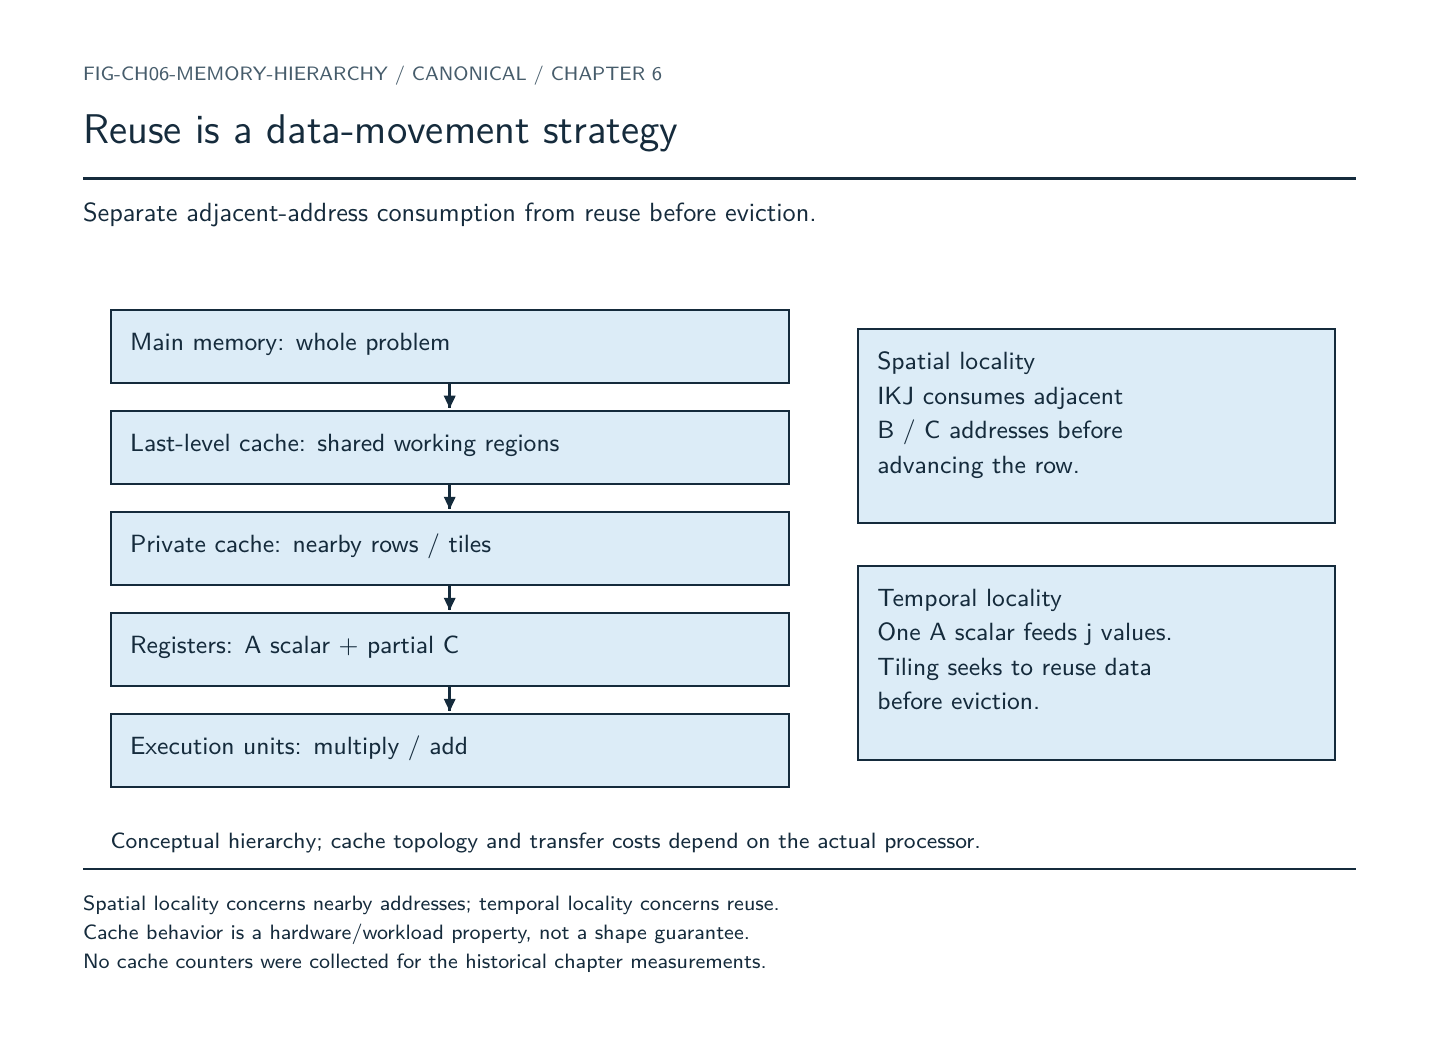
\begin{tikzpicture}[x=.5pt,y=-.5pt]
\path[use as bounding box] (0,0) rectangle (1000,720);
\path[fill=white,draw=none,line width=0.5pt] (0.0,0.0) rectangle (1000.0,720.0);
\node[inner sep=0pt,outer sep=0pt,anchor=base west,text={rgb,255:red,70;green,92;blue,107},font=\sffamily\fontsize{7.0}{8.4}\selectfont] at (40,38) {FIG-CH06-MEMORY-HIERARCHY  /  CANONICAL / CHAPTER 6};
\node[inner sep=0pt,outer sep=0pt,anchor=base west,text={rgb,255:red,21;green,43;blue,60},font=\sffamily\fontsize{15.0}{18.0}\selectfont] at (40,84) {Reuse is a data-movement strategy};
\draw[fill=none,draw={rgb,255:red,21;green,43;blue,60},line width=0.75pt] (40,109) -- (960,109);
\node[inner sep=0pt,outer sep=0pt,anchor=base west,text={rgb,255:red,21;green,43;blue,60},font=\sffamily\fontsize{9.5}{11.4}\selectfont] at (40,140) {Separate adjacent-address consumption from reuse before eviction.};
\path[fill={rgb,255:red,220;green,236;blue,247},draw={rgb,255:red,21;green,43;blue,60},line width=0.7pt] (60.0,204.0) rectangle (550.0,257.0);
\node[inner sep=0pt,outer sep=0pt,anchor=base west,text={rgb,255:red,21;green,43;blue,60},font=\sffamily\fontsize{9.0}{10.799999999999999}\selectfont] at (74,233) {Main memory: whole problem};
\node[inner sep=0pt,outer sep=0pt,anchor=base west,text={rgb,255:red,21;green,43;blue,60},font=\sffamily\fontsize{9.0}{10.799999999999999}\selectfont] at (74,258) {};
\draw[fill=none,draw={rgb,255:red,21;green,43;blue,60},line width=1.25pt] (305,257) -- (305,275);
\path[fill={rgb,255:red,21;green,43;blue,60},draw=none,line width=0.5pt] (305.00,275.00) -- (300.65,266.00) -- (309.35,266.00) -- cycle;
\path[fill={rgb,255:red,220;green,236;blue,247},draw={rgb,255:red,21;green,43;blue,60},line width=0.7pt] (60.0,277.0) rectangle (550.0,330.0);
\node[inner sep=0pt,outer sep=0pt,anchor=base west,text={rgb,255:red,21;green,43;blue,60},font=\sffamily\fontsize{9.0}{10.799999999999999}\selectfont] at (74,306) {Last-level cache: shared working regions};
\node[inner sep=0pt,outer sep=0pt,anchor=base west,text={rgb,255:red,21;green,43;blue,60},font=\sffamily\fontsize{9.0}{10.799999999999999}\selectfont] at (74,331) {};
\draw[fill=none,draw={rgb,255:red,21;green,43;blue,60},line width=1.25pt] (305,330) -- (305,348);
\path[fill={rgb,255:red,21;green,43;blue,60},draw=none,line width=0.5pt] (305.00,348.00) -- (300.65,339.00) -- (309.35,339.00) -- cycle;
\path[fill={rgb,255:red,220;green,236;blue,247},draw={rgb,255:red,21;green,43;blue,60},line width=0.7pt] (60.0,350.0) rectangle (550.0,403.0);
\node[inner sep=0pt,outer sep=0pt,anchor=base west,text={rgb,255:red,21;green,43;blue,60},font=\sffamily\fontsize{9.0}{10.799999999999999}\selectfont] at (74,379) {Private cache: nearby rows / tiles};
\node[inner sep=0pt,outer sep=0pt,anchor=base west,text={rgb,255:red,21;green,43;blue,60},font=\sffamily\fontsize{9.0}{10.799999999999999}\selectfont] at (74,404) {};
\draw[fill=none,draw={rgb,255:red,21;green,43;blue,60},line width=1.25pt] (305,403) -- (305,421);
\path[fill={rgb,255:red,21;green,43;blue,60},draw=none,line width=0.5pt] (305.00,421.00) -- (300.65,412.00) -- (309.35,412.00) -- cycle;
\path[fill={rgb,255:red,220;green,236;blue,247},draw={rgb,255:red,21;green,43;blue,60},line width=0.7pt] (60.0,423.0) rectangle (550.0,476.0);
\node[inner sep=0pt,outer sep=0pt,anchor=base west,text={rgb,255:red,21;green,43;blue,60},font=\sffamily\fontsize{9.0}{10.799999999999999}\selectfont] at (74,452) {Registers: A scalar + partial C};
\node[inner sep=0pt,outer sep=0pt,anchor=base west,text={rgb,255:red,21;green,43;blue,60},font=\sffamily\fontsize{9.0}{10.799999999999999}\selectfont] at (74,477) {};
\draw[fill=none,draw={rgb,255:red,21;green,43;blue,60},line width=1.25pt] (305,476) -- (305,494);
\path[fill={rgb,255:red,21;green,43;blue,60},draw=none,line width=0.5pt] (305.00,494.00) -- (300.65,485.00) -- (309.35,485.00) -- cycle;
\path[fill={rgb,255:red,220;green,236;blue,247},draw={rgb,255:red,21;green,43;blue,60},line width=0.7pt] (60.0,496.0) rectangle (550.0,549.0);
\node[inner sep=0pt,outer sep=0pt,anchor=base west,text={rgb,255:red,21;green,43;blue,60},font=\sffamily\fontsize{9.0}{10.799999999999999}\selectfont] at (74,525) {Execution units: multiply / add};
\node[inner sep=0pt,outer sep=0pt,anchor=base west,text={rgb,255:red,21;green,43;blue,60},font=\sffamily\fontsize{9.0}{10.799999999999999}\selectfont] at (74,550) {};
\path[fill={rgb,255:red,220;green,236;blue,247},draw={rgb,255:red,21;green,43;blue,60},line width=0.7pt] (600.0,218.0) rectangle (945.0,358.0);
\node[inner sep=0pt,outer sep=0pt,anchor=base west,text={rgb,255:red,21;green,43;blue,60},font=\sffamily\fontsize{9.0}{10.799999999999999}\selectfont] at (614,247) {Spatial locality};
\node[inner sep=0pt,outer sep=0pt,anchor=base west,text={rgb,255:red,21;green,43;blue,60},font=\sffamily\fontsize{9.0}{10.799999999999999}\selectfont] at (614,272) {IKJ consumes adjacent};
\node[inner sep=0pt,outer sep=0pt,anchor=base west,text={rgb,255:red,21;green,43;blue,60},font=\sffamily\fontsize{9.0}{10.799999999999999}\selectfont] at (614,297) {B / C addresses before};
\node[inner sep=0pt,outer sep=0pt,anchor=base west,text={rgb,255:red,21;green,43;blue,60},font=\sffamily\fontsize{9.0}{10.799999999999999}\selectfont] at (614,322) {advancing the row.};
\path[fill={rgb,255:red,220;green,236;blue,247},draw={rgb,255:red,21;green,43;blue,60},line width=0.7pt] (600.0,389.0) rectangle (945.0,529.0);
\node[inner sep=0pt,outer sep=0pt,anchor=base west,text={rgb,255:red,21;green,43;blue,60},font=\sffamily\fontsize{9.0}{10.799999999999999}\selectfont] at (614,418) {Temporal locality};
\node[inner sep=0pt,outer sep=0pt,anchor=base west,text={rgb,255:red,21;green,43;blue,60},font=\sffamily\fontsize{9.0}{10.799999999999999}\selectfont] at (614,443) {One A scalar feeds j values.};
\node[inner sep=0pt,outer sep=0pt,anchor=base west,text={rgb,255:red,21;green,43;blue,60},font=\sffamily\fontsize{9.0}{10.799999999999999}\selectfont] at (614,468) {Tiling seeks to reuse data};
\node[inner sep=0pt,outer sep=0pt,anchor=base west,text={rgb,255:red,21;green,43;blue,60},font=\sffamily\fontsize{9.0}{10.799999999999999}\selectfont] at (614,493) {before eviction.};
\node[inner sep=0pt,outer sep=0pt,anchor=base west,text={rgb,255:red,21;green,43;blue,60},font=\sffamily\fontsize{8.0}{9.6}\selectfont] at (60,593) {Conceptual hierarchy; cache topology and transfer costs depend on the actual processor.};
\draw[fill=none,draw={rgb,255:red,21;green,43;blue,60},line width=0.75pt] (40,608) -- (960,608);
\node[inner sep=0pt,outer sep=0pt,anchor=base west,text={rgb,255:red,21;green,43;blue,60},font=\sffamily\fontsize{7.5}{9.0}\selectfont] at (40,638) {Spatial locality concerns nearby addresses; temporal locality concerns reuse.};
\node[inner sep=0pt,outer sep=0pt,anchor=base west,text={rgb,255:red,21;green,43;blue,60},font=\sffamily\fontsize{7.5}{9.0}\selectfont] at (40,659) {Cache behavior is a hardware/workload property, not a shape guarantee.};
\node[inner sep=0pt,outer sep=0pt,anchor=base west,text={rgb,255:red,21;green,43;blue,60},font=\sffamily\fontsize{7.5}{9.0}\selectfont] at (40,680) {No cache counters were collected for the historical chapter measurements.};
\end{tikzpicture}
}\caption{Conceptual memory-to-execution hierarchy with spatial and temporal locality distinguished.}\end{figure}

A processor does not generally load every scalar directly from main
memory on every use. Registers sit closest to arithmetic. Several cache
levels retain recently accessed lines. Main memory is larger and usually
more expensive to reach. Exact capacities, policies, and latencies are
architecture-specific, but the hierarchy creates a general objective:
arrange work so values are reused while they remain in a faster level.

The \textbf{working set} is the data actively needed during a region of
execution. For one output cell in \texttt{ijk}, the conceptual set
includes an A row, a B column, and one accumulator. The A row has a
contiguous walk, but the B column touches many separated cache lines
when N is large. Across adjacent output columns, the algorithm revisits
the same A row, yet whether it remains resident depends on the rest of
the active footprint.

In \texttt{ikj}, one \(A_{ik}\) scalar is loaded into a local variable
and reused across an output row. The active B row and C row are
contiguous. This does not ensure that an entire long row fits a
particular cache, but it exposes short-range spatial reuse to the
hardware and compiler.

Blocking shrinks that focus again. Instead of streaming complete rows
while other operands compete for capacity, it asks the machine to
revisit bounded A, B, and C regions. A useful tile lets multiple
arithmetic contributions occur per line fetched from a lower level. A
bad tile can be too large to retain, too small to amortize control, or
poorly shaped for the matrix.

Cache lines also explain why counting logical scalar loads in source is
not a traffic measurement. Loading one \texttt{f32} can bring
neighboring values. A later access may hit that line without another
main-memory transfer, or the line may have been evicted and fetched
again. The minimum-byte equations describe data that must logically
participate; only appropriate performance counters and a defined
hierarchy boundary could establish physical bytes.

This distinction prevents a common reasoning error. We may say
\texttt{ikj} presents contiguous B access and that blocking is designed
to increase temporal reuse. We may not say exactly how many cache misses
it removes on the recorded host, because the current benchmark records
elapsed time rather than cache events.

There are six permutations of three distinct loop indices:

\begin{verbatim}
ijk   ikj   jik   jki   kij   kji
\end{verbatim}

Not all can use a single scalar accumulator in the same way, and their
access patterns differ under row-major layout. ENGINE-2 studies
\texttt{ijk} and \texttt{ikj} rather than pretending to rank all six
universally.

\subsection{\texorpdfstring{The \texttt{ikj}
rewrite}{The ikj rewrite}}\label{the-ikj-rewrite}

The update equation can be written as

\[
C_{ij}\mathrel{+}=A_{ik}B_{kj}.
\]

For a fixed \(i\) and \(k\), let \(j\) vary through a row segment:

\begin{verbatim}
for i in 0..m {
    for k in 0..inner {
        let left_value = left[i * inner + k];
        for j in 0..n {
            output[i * n + j] += left_value * right[k * n + j];
        }
    }
}
\end{verbatim}

Now the innermost loop walks adjacent \(B_{kj}\) and \(C_{ij}\)
positions. One loaded \(A_{ik}\) scalar feeds an entire output-row
segment. The canonical
\href{https://github.com/hermonai/inside-the-llm-engine/blob/astra-visual-rewrite/diagrams/linear/loop-order-ijk-vs-ikj.txt}{loop-order
diagram} and
\href{https://github.com/hermonai/inside-the-llm-engine/blob/astra-visual-rewrite/diagrams/linear/follow-the-reuse.txt}{reuse
diagram} show this change.

Initialization moved too. \texttt{ijk} can compute one local sum and
assign a cell. \texttt{ikj} accumulates into many cells across K
iterations, so the output must be zero-initialized before the loop.
Forgetting that step produces dependence on old storage rather than
matrix multiplication.

\begin{quote}
\textbf{PERFORMANCE LAB}
\href{https://github.com/hermonai/inside-the-llm-engine/blob/astra-visual-rewrite/labs/lab-25-loop-order.md}{Lab
25} begins with physical offset sequences, not a stopwatch. Correctness
is the admission ticket to timing.
\end{quote}

\subsection{Performance lab: loop
order}\label{performance-lab-loop-order}

\begin{figure}[H]\centering\resizebox{\linewidth}{!}{% Generated from figures/generated/ch06-loops.svg; do not hand edit.
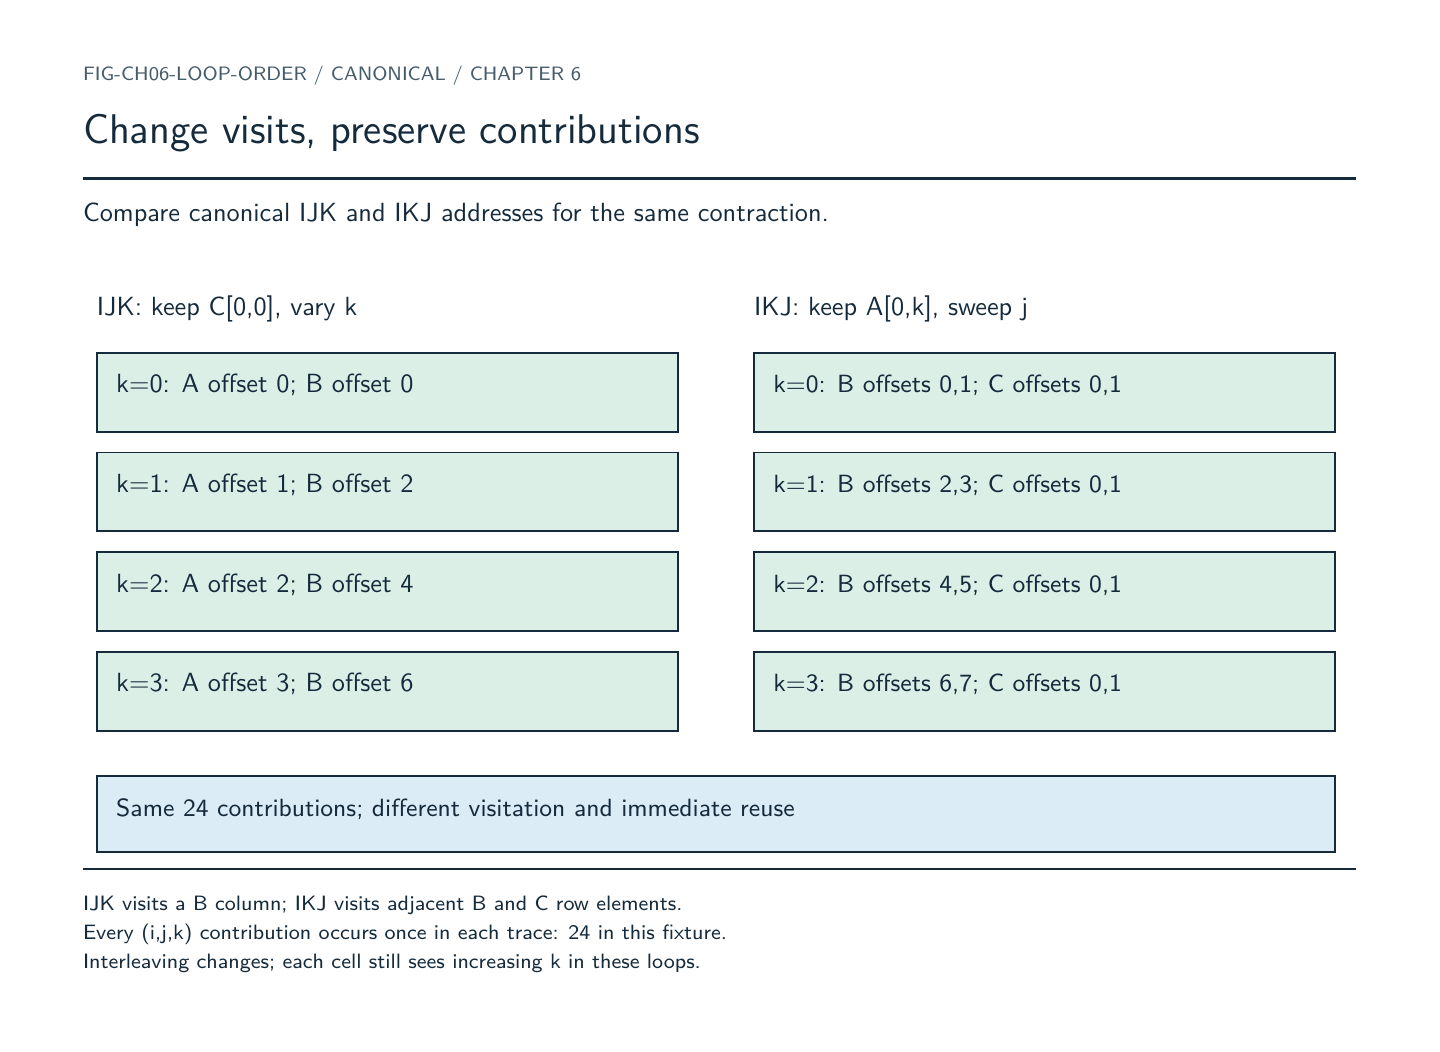
\begin{tikzpicture}[x=.5pt,y=-.5pt]
\path[use as bounding box] (0,0) rectangle (1000,720);
\path[fill=white,draw=none,line width=0.5pt] (0.0,0.0) rectangle (1000.0,720.0);
\node[inner sep=0pt,outer sep=0pt,anchor=base west,text={rgb,255:red,70;green,92;blue,107},font=\sffamily\fontsize{7.0}{8.4}\selectfont] at (40,38) {FIG-CH06-LOOP-ORDER  /  CANONICAL / CHAPTER 6};
\node[inner sep=0pt,outer sep=0pt,anchor=base west,text={rgb,255:red,21;green,43;blue,60},font=\sffamily\fontsize{15.0}{18.0}\selectfont] at (40,84) {Change visits, preserve contributions};
\draw[fill=none,draw={rgb,255:red,21;green,43;blue,60},line width=0.75pt] (40,109) -- (960,109);
\node[inner sep=0pt,outer sep=0pt,anchor=base west,text={rgb,255:red,21;green,43;blue,60},font=\sffamily\fontsize{9.5}{11.4}\selectfont] at (40,140) {Compare canonical IJK and IKJ addresses for the same contraction.};
\node[inner sep=0pt,outer sep=0pt,anchor=base west,text={rgb,255:red,21;green,43;blue,60},font=\sffamily\fontsize{9.5}{11.4}\selectfont] at (50,208) {IJK: keep C[0,0], vary k};
\node[inner sep=0pt,outer sep=0pt,anchor=base west,text={rgb,255:red,21;green,43;blue,60},font=\sffamily\fontsize{9.5}{11.4}\selectfont] at (525,208) {IKJ: keep A[0,k], sweep j};
\path[fill={rgb,255:red,220;green,239;blue,231},draw={rgb,255:red,21;green,43;blue,60},line width=0.7pt] (50.0,235.0) rectangle (470.0,292.0);
\node[inner sep=0pt,outer sep=0pt,anchor=base west,text={rgb,255:red,21;green,43;blue,60},font=\sffamily\fontsize{9.5}{11.4}\selectfont] at (64,264) {k=0: A offset 0; B offset 0};
\path[fill={rgb,255:red,220;green,239;blue,231},draw={rgb,255:red,21;green,43;blue,60},line width=0.7pt] (525.0,235.0) rectangle (945.0,292.0);
\node[inner sep=0pt,outer sep=0pt,anchor=base west,text={rgb,255:red,21;green,43;blue,60},font=\sffamily\fontsize{9.0}{10.799999999999999}\selectfont] at (539,264) {k=0: B offsets 0,1; C offsets 0,1};
\path[fill={rgb,255:red,220;green,239;blue,231},draw={rgb,255:red,21;green,43;blue,60},line width=0.7pt] (50.0,307.0) rectangle (470.0,364.0);
\node[inner sep=0pt,outer sep=0pt,anchor=base west,text={rgb,255:red,21;green,43;blue,60},font=\sffamily\fontsize{9.5}{11.4}\selectfont] at (64,336) {k=1: A offset 1; B offset 2};
\path[fill={rgb,255:red,220;green,239;blue,231},draw={rgb,255:red,21;green,43;blue,60},line width=0.7pt] (525.0,307.0) rectangle (945.0,364.0);
\node[inner sep=0pt,outer sep=0pt,anchor=base west,text={rgb,255:red,21;green,43;blue,60},font=\sffamily\fontsize{9.0}{10.799999999999999}\selectfont] at (539,336) {k=1: B offsets 2,3; C offsets 0,1};
\path[fill={rgb,255:red,220;green,239;blue,231},draw={rgb,255:red,21;green,43;blue,60},line width=0.7pt] (50.0,379.0) rectangle (470.0,436.0);
\node[inner sep=0pt,outer sep=0pt,anchor=base west,text={rgb,255:red,21;green,43;blue,60},font=\sffamily\fontsize{9.5}{11.4}\selectfont] at (64,408) {k=2: A offset 2; B offset 4};
\path[fill={rgb,255:red,220;green,239;blue,231},draw={rgb,255:red,21;green,43;blue,60},line width=0.7pt] (525.0,379.0) rectangle (945.0,436.0);
\node[inner sep=0pt,outer sep=0pt,anchor=base west,text={rgb,255:red,21;green,43;blue,60},font=\sffamily\fontsize{9.0}{10.799999999999999}\selectfont] at (539,408) {k=2: B offsets 4,5; C offsets 0,1};
\path[fill={rgb,255:red,220;green,239;blue,231},draw={rgb,255:red,21;green,43;blue,60},line width=0.7pt] (50.0,451.0) rectangle (470.0,508.0);
\node[inner sep=0pt,outer sep=0pt,anchor=base west,text={rgb,255:red,21;green,43;blue,60},font=\sffamily\fontsize{9.5}{11.4}\selectfont] at (64,480) {k=3: A offset 3; B offset 6};
\path[fill={rgb,255:red,220;green,239;blue,231},draw={rgb,255:red,21;green,43;blue,60},line width=0.7pt] (525.0,451.0) rectangle (945.0,508.0);
\node[inner sep=0pt,outer sep=0pt,anchor=base west,text={rgb,255:red,21;green,43;blue,60},font=\sffamily\fontsize{9.0}{10.799999999999999}\selectfont] at (539,480) {k=3: B offsets 6,7; C offsets 0,1};
\path[fill={rgb,255:red,220;green,236;blue,247},draw={rgb,255:red,21;green,43;blue,60},line width=0.7pt] (50.0,541.0) rectangle (945.0,596.0);
\node[inner sep=0pt,outer sep=0pt,anchor=base west,text={rgb,255:red,21;green,43;blue,60},font=\sffamily\fontsize{9.0}{10.799999999999999}\selectfont] at (64,570) {Same 24 contributions; different visitation and immediate reuse};
\node[inner sep=0pt,outer sep=0pt,anchor=base west,text={rgb,255:red,21;green,43;blue,60},font=\sffamily\fontsize{9.0}{10.799999999999999}\selectfont] at (64,595) {};
\draw[fill=none,draw={rgb,255:red,21;green,43;blue,60},line width=0.75pt] (40,608) -- (960,608);
\node[inner sep=0pt,outer sep=0pt,anchor=base west,text={rgb,255:red,21;green,43;blue,60},font=\sffamily\fontsize{7.5}{9.0}\selectfont] at (40,638) {IJK visits a B column; IKJ visits adjacent B and C row elements.};
\node[inner sep=0pt,outer sep=0pt,anchor=base west,text={rgb,255:red,21;green,43;blue,60},font=\sffamily\fontsize{7.5}{9.0}\selectfont] at (40,659) {Every (i,j,k) contribution occurs once in each trace: 24 in this fixture.};
\node[inner sep=0pt,outer sep=0pt,anchor=base west,text={rgb,255:red,21;green,43;blue,60},font=\sffamily\fontsize{7.5}{9.0}\selectfont] at (40,680) {Interleaving changes; each cell still sees increasing k in these loops.};
\end{tikzpicture}
}\caption{IJK strides down B while IKJ sweeps adjacent B and C elements, preserving all contributions.}\end{figure}

For the fixture, canonical strides are \texttt{A:{[}4,1{]}},
\texttt{B:{[}2,1{]}}, \texttt{C:{[}2,1{]}}. At \texttt{i=0,j=0}, IJK
reads B offsets \texttt{0,2,4,6}; IKJ at \texttt{i=0,k=0} reads offsets
\texttt{0,1} and updates C offsets \texttt{0,1} using the same A scalar.
The
\href{https://github.com/hermonai/inside-the-llm-engine/blob/astra-visual-rewrite/figures/generated/ch06-loops.html}{loop-order
animation} advances \(k\); its static plate shows all four states. The
parity gate verifies that the full IJK and IKJ traces contain the
identical set of 24 \texttt{(i,j,k)} contributions. This proves
traversal coverage, not a cache-hit count or a speedup.

The release harness compares direct scalar row-major \texttt{ijk} and
\texttt{ikj} loops. Both allocate and zero their result, use
deterministic \texttt{f32} inputs, and pass a per-element correctness
gate. On the recorded Apple M1 run at code commit \texttt{03e08a87}
(full pin in the record), median results were:

{\def\LTcaptype{none} % do not increment counter
\begin{longtable}[]{@{}rrrrr@{}}
\toprule\noalign{}
Square size & Repetitions & \texttt{ijk} & \texttt{ikj} & Observed
ratio \\
\midrule\noalign{}
\endhead
\bottomrule\noalign{}
\endlastfoot
64 & 15 & 185,375 ns & 54,791 ns & 3.38× \\
128 & 9 & 1,645,000 ns & 286,375 ns & 5.74× \\
256 & 5 & 15,638,708 ns & 1,709,000 ns & 9.15× \\
\end{longtable}
}

The exact environment, command, raw checksums, compiler, and limitations
live in the
\href{https://github.com/hermonai/inside-the-llm-engine/blob/astra-visual-rewrite/research/benchmarks/chapter-06-loop-order.md}{loop-order
benchmark record}. For these tested shapes, \texttt{ikj} had the lower
median. The widening ratio is consistent with its contiguous inner
walks; it is not a portable law or a substitute for hardware-counter
evidence.

\subsection{What the benchmark does---and does
not---measure}\label{what-the-benchmark-doesand-does-notmeasure}

The Chapter 6 harness uses \texttt{\seqsplit{std::time::Instant}} in a
Cargo release build. Inputs are deterministically generated before
timing. Every candidate is executed once for correctness before samples
are accepted. Timed output is consumed through a checksum and
\texttt{black\_box}, reducing the chance that an optimizing compiler
discards the work. Samples are sorted and the median is reported.

Median is a defensible summary for this bounded, exploratory
microbenchmark, but it does not describe tail latency or serving
variability. Repetition counts appear beside every result. Small shapes
use more repetitions because each sample is short; larger shapes use
fewer to keep the exercise practical. The process is warm, but cache
contents are not flushed or controlled between samples. Candidate order
is stable rather than randomized. Frequency, temperature,
operating-system activity, and compiler-generated instructions are not
independently measured.

Allocation and zero-initialization are included. That matches the
current public API, which returns a fresh \texttt{OwnedTensor}, and
prevents a prepared-output control from receiving a hidden advantage. It
also means the record cannot attribute every nanosecond to arithmetic or
cache traversal. A future reusable output API would require a separate
experiment with equivalent initialization policy.

The harness's direct \texttt{ijk} and \texttt{ikj} functions use
canonical flat slices after their deterministic construction. Timing
\texttt{\seqsplit{matmul\_reference}} itself would also include a
checked logical view lookup for every operand access, confounding the
loop-order question with repeated boundary validation. Correctness still
uses the public contracts; the loop-order experiment isolates the two
flat scalar traversals. The blocked experiments time the actual public
blocked kernel, including its metadata views and layout checks.

Effective GFLOP/s divides the conventional work estimate by elapsed
time. It is useful for comparing shapes inside this record, but it is
not measured peak hardware throughput. The ideal FLOP/byte column
divides work by compulsory logical payload, not hardware counters.
Publishing both without these labels would create precision without
accuracy.

Finally, the benchmark is not an inference benchmark. It has no
tokenizer, request queue, model file, KV cache, sampling, streaming,
concurrency, or token latency. Its purpose is narrower: make one kernel
hypothesis reproducible. End- to-end claims require end-to-end workloads
and cannot be obtained by multiplying independent microbenchmark ratios.

\subsection{Memory movement}\label{memory-movement}

A simplistic implementation might reload \(A_{ik}\) and \(B_{kj}\) for
every mathematical contribution, then repeatedly read and write
\(C_{ij}\). Caches can remove some transfers to lower memory levels, but
only if the active data stays resident and the access order exposes
reuse.

The smallest compulsory payload model for canonical \texttt{f32} GEMM
reads each input once and writes each output once:

\[
Q_{\min}=4(MK+KN+MN)\quad[\mathrm{bytes}].
\]

This is a lower-bound model, not measured traffic. Write allocation,
eviction, cache-line granularity, repeated loads, and metadata can
increase physical movement. The
\href{https://github.com/hermonai/inside-the-llm-engine/blob/astra-visual-rewrite/diagrams/linear/follow-the-byte.txt}{byte-flow
diagram} keeps the ownership and transfer story separate from the
formula.

\subsection{Arithmetic intensity}\label{arithmetic-intensity}

\textbf{Arithmetic intensity} is floating-point work divided by bytes
moved at a chosen memory boundary:

\[
I=\frac{F}{Q}\quad[\mathrm{FLOP/byte}].
\]

Using the compulsory-payload model for GEMM gives

\[
I_{\mathrm{ideal}}
\approx\frac{2MKN}{4(MK+KN+MN)}\quad[\mathrm{FLOP/byte}].
\]

The word \emph{ideal} is essential. Without hardware counters, ENGINE-2
does not know actual cache or DRAM traffic.

For GEMV with \(A:[M,K]\), \(x:[K]\), and \(y:[M]\), the analogous model
is

\[
I_{\mathrm{GEMV,ideal}}
\approx\frac{2MK}{4(MK+K+M)}\quad[\mathrm{FLOP/byte}].
\]

For large \(M\) and \(K\), the \(MK\) weight term dominates, so
intensity approaches approximately \(0.5\) FLOP/byte. One weight
contributes to one output vector. In GEMM, a weight can contribute
across \(N\) columns, so potential reuse and ideal intensity grow with
\(N\).

\subsubsection{Future connection: prefill and
decode}\label{future-connection-prefill-and-decode}

Later chapters will distinguish two inference workload phases.
\textbf{Prefill} processes many prompt positions and can present
matrix-like collections of activations. \textbf{Decode} advances one or
a few new positions per active sequence and can present vector-like or
skinny-matrix work. That suggests a useful first intuition:

\begin{center}\begin{adjustbox}{max width=\linewidth}% Legacy topology preserved as native vectors and typeset labels.
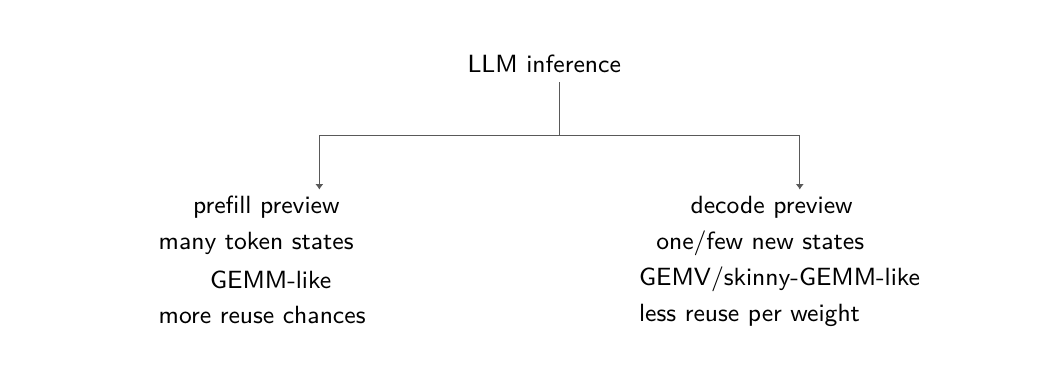
\begin{tikzpicture}[x=6.2pt,y=-13pt,draw=black!65,line width=.45pt]
\path[use as bounding box] (-1,-1) rectangle (57,8);
\node[anchor=west,inner sep=0pt,font=\sffamily\fontsize{9}{11}\selectfont] at (24.6,0) {\begin{adjustbox}{max width=80.60000000000001pt}LLM inference\end{adjustbox}};
\draw (30,1) -- (30,0.5);
\draw (30,1) -- (30,1.5);
\draw (16,2) -- (16.5,2);
\draw (16,2) -- (16,2.5);
\draw (17,2) -- (16.5,2);
\draw (17,2) -- (17.5,2);
\draw (18,2) -- (17.5,2);
\draw (18,2) -- (18.5,2);
\draw (19,2) -- (18.5,2);
\draw (19,2) -- (19.5,2);
\draw (20,2) -- (19.5,2);
\draw (20,2) -- (20.5,2);
\draw (21,2) -- (20.5,2);
\draw (21,2) -- (21.5,2);
\draw (22,2) -- (21.5,2);
\draw (22,2) -- (22.5,2);
\draw (23,2) -- (22.5,2);
\draw (23,2) -- (23.5,2);
\draw (24,2) -- (23.5,2);
\draw (24,2) -- (24.5,2);
\draw (25,2) -- (24.5,2);
\draw (25,2) -- (25.5,2);
\draw (26,2) -- (25.5,2);
\draw (26,2) -- (26.5,2);
\draw (27,2) -- (26.5,2);
\draw (27,2) -- (27.5,2);
\draw (28,2) -- (27.5,2);
\draw (28,2) -- (28.5,2);
\draw (29,2) -- (28.5,2);
\draw (29,2) -- (29.5,2);
\draw (30,2) -- (29.5,2);
\draw (30,2) -- (30.5,2);
\draw (30,2) -- (30,1.5);
\draw (31,2) -- (30.5,2);
\draw (31,2) -- (31.5,2);
\draw (32,2) -- (31.5,2);
\draw (32,2) -- (32.5,2);
\draw (33,2) -- (32.5,2);
\draw (33,2) -- (33.5,2);
\draw (34,2) -- (33.5,2);
\draw (34,2) -- (34.5,2);
\draw (35,2) -- (34.5,2);
\draw (35,2) -- (35.5,2);
\draw (36,2) -- (35.5,2);
\draw (36,2) -- (36.5,2);
\draw (37,2) -- (36.5,2);
\draw (37,2) -- (37.5,2);
\draw (38,2) -- (37.5,2);
\draw (38,2) -- (38.5,2);
\draw (39,2) -- (38.5,2);
\draw (39,2) -- (39.5,2);
\draw (40,2) -- (39.5,2);
\draw (40,2) -- (40.5,2);
\draw (41,2) -- (40.5,2);
\draw (41,2) -- (41.5,2);
\draw (42,2) -- (41.5,2);
\draw (42,2) -- (42.5,2);
\draw (43,2) -- (42.5,2);
\draw (43,2) -- (43.5,2);
\draw (44,2) -- (43.5,2);
\draw (44,2) -- (44,2.5);
\draw[-{Latex[length=2pt,width=3pt]}] (16,2.5) -- (16,3.5);
\draw[-{Latex[length=2pt,width=3pt]}] (44,2.5) -- (44,3.5);
\node[anchor=west,inner sep=0pt,font=\sffamily\fontsize{9}{11}\selectfont] at (8.6,4) {\begin{adjustbox}{max width=93.0pt}prefill preview\end{adjustbox}};
\node[anchor=west,inner sep=0pt,font=\sffamily\fontsize{9}{11}\selectfont] at (37.6,4) {\begin{adjustbox}{max width=86.8pt}decode preview\end{adjustbox}};
\node[anchor=west,inner sep=0pt,font=\sffamily\fontsize{9}{11}\selectfont] at (6.6,5) {\begin{adjustbox}{max width=105.4pt}many token states\end{adjustbox}};
\node[anchor=west,inner sep=0pt,font=\sffamily\fontsize{9}{11}\selectfont] at (35.6,5) {\begin{adjustbox}{max width=111.60000000000001pt}one/few new states\end{adjustbox}};
\node[anchor=west,inner sep=0pt,font=\sffamily\fontsize{9}{11}\selectfont] at (9.6,6) {\begin{adjustbox}{max width=55.800000000000004pt}GEMM-like\end{adjustbox}};
\node[anchor=west,inner sep=0pt,font=\sffamily\fontsize{9}{11}\selectfont] at (34.6,6) {\begin{adjustbox}{max width=130.20000000000002pt}GEMV/skinny-GEMM-like\end{adjustbox}};
\node[anchor=west,inner sep=0pt,font=\sffamily\fontsize{9}{11}\selectfont] at (6.6,7) {\begin{adjustbox}{max width=111.60000000000001pt}more reuse chances\end{adjustbox}};
\node[anchor=west,inner sep=0pt,font=\sffamily\fontsize{9}{11}\selectfont] at (34.6,7) {\begin{adjustbox}{max width=130.20000000000002pt}less reuse per weight\end{adjustbox}};
\end{tikzpicture}
\end{adjustbox}\end{center}

This is explicitly a conceptual preview, not a complete workload model.
Attention shapes, batching, KV state, quantization, providers, and
scheduling will refine it. A production runtime may also batch decode
work from several requests into a matrix. Chapter 6 establishes only the
numerical reason that the number of activation columns can change
weight-reuse opportunity.

\subsection{The Roofline mental model}\label{the-roofline-mental-model}

The Roofline model relates attainable performance to peak compute,
memory bandwidth, and arithmetic intensity:

\[
P\le\min\left(P_{\mathrm{peak}},\ B_{\mathrm{memory}}I\right).
\]

At low intensity, the sloped bandwidth term can be the tighter ceiling.
At high intensity, the horizontal compute ceiling can dominate. The
canonical
\href{https://github.com/hermonai/inside-the-llm-engine/blob/astra-visual-rewrite/diagrams/linear/roofline-concept.txt}{Roofline
concept diagram} is a mental model, not a calibrated roofline for this
laptop. We have not measured peak bandwidth, peak arithmetic throughput,
or per-level traffic.

This preview answers the chapter's central question: multiplication may
be cheap relative to repeatedly delivering its operands. An optimization
can improve performance without changing FLOPs if it improves realized
data reuse. Conversely, a theoretically higher-intensity workload can
remain slow when a poor scalar kernel fails to exploit that opportunity.

\subsection{Why blocking exists}\label{why-blocking-exists}

Loop interchange improves the immediate access direction, but whole rows
or matrices can still exceed a fast cache. \textbf{Blocking}, also
called \textbf{tiling}, partitions M, K, and N into bounded ranges. The
kernel works on an \(A\) tile, a \(B\) tile, and an accumulating \(C\)
tile before moving on.

The
\href{https://github.com/hermonai/inside-the-llm-engine/blob/astra-visual-rewrite/diagrams/linear/cache-reuse-and-tiling.txt}{tiling
diagram} shows the intended active set. For block extents
\((B_M,B_K,B_N)\), one rough \texttt{f32} payload is

\[
Q_{\mathrm{tile}}=4(B_MB_K+B_KB_N+B_MB_N)\quad[\mathrm{bytes}].
\]

That formula does not select a universally correct tile. Cache capacity
is not the only constraint: associativity, cache lines, register
pressure, loop overhead, compiler decisions, and matrix shape all
matter. ENGINE-2 makes the three extents explicit and offers
\texttt{{[}32,32,32{]}} as a teaching default, not a machine truth.

\subsection{Build it: blocked scalar
GEMM}\label{build-it-blocked-scalar-gemm}

The blocked path uses outer tile loops \texttt{ii,kk,jj} and inner
scalar loops \texttt{i,k,j}. This is the actual loop body from
\texttt{linear.rs}, after validation and zero-initialized output
allocation:

\begin{verbatim}
for ii in (0..rows).step_by(block.m) {
    let i_end = ii.saturating_add(block.m).min(rows);
    for kk in (0..inner).step_by(block.k) {
        let k_end = kk.saturating_add(block.k).min(inner);
        for jj in (0..columns).step_by(block.n) {
            let j_end = jj.saturating_add(block.n).min(columns);
            for i in ii..i_end {
                let output_row = i * columns;
                let left_row = i * inner;
                for k in kk..k_end {
                    let left_value = left_data[left_row + k];
                    let right_row = k * columns;
                    for j in jj..j_end {
                        output[output_row + j] += left_value * right_data[right_row + j];
                    }
                }
            }
        }
    }
}
\end{verbatim}

The real implementation uses saturating addition before \texttt{min} so
even endpoint arithmetic cannot wrap. Each block extent must be
positive; otherwise \texttt{step\_by(0)} would be invalid and the
intended partition would be meaningless.

Tail tiles are mandatory. For \texttt{{[}5,7{]}\ ×\ {[}7,3{]}} with
blocks \texttt{{[}4,4,2{]}}, all three axes have a partial final tile. A
benchmark that tests only dimensions evenly divisible by the block size
can report a fast but incomplete kernel.

\begin{quote}
\textbf{BUILD IT}
\href{https://github.com/hermonai/inside-the-llm-engine/blob/astra-visual-rewrite/labs/lab-26-blocked-gemm.md}{Lab
26} traces those three tails and compares every result cell with the
reference path.
\end{quote}

\subsection{Separate checked boundary from hot
loop}\label{separate-checked-boundary-from-hot-loop}

\begin{figure}[H]\centering\resizebox{\linewidth}{!}{% Generated from figures/generated/ch06-tiles.svg; do not hand edit.
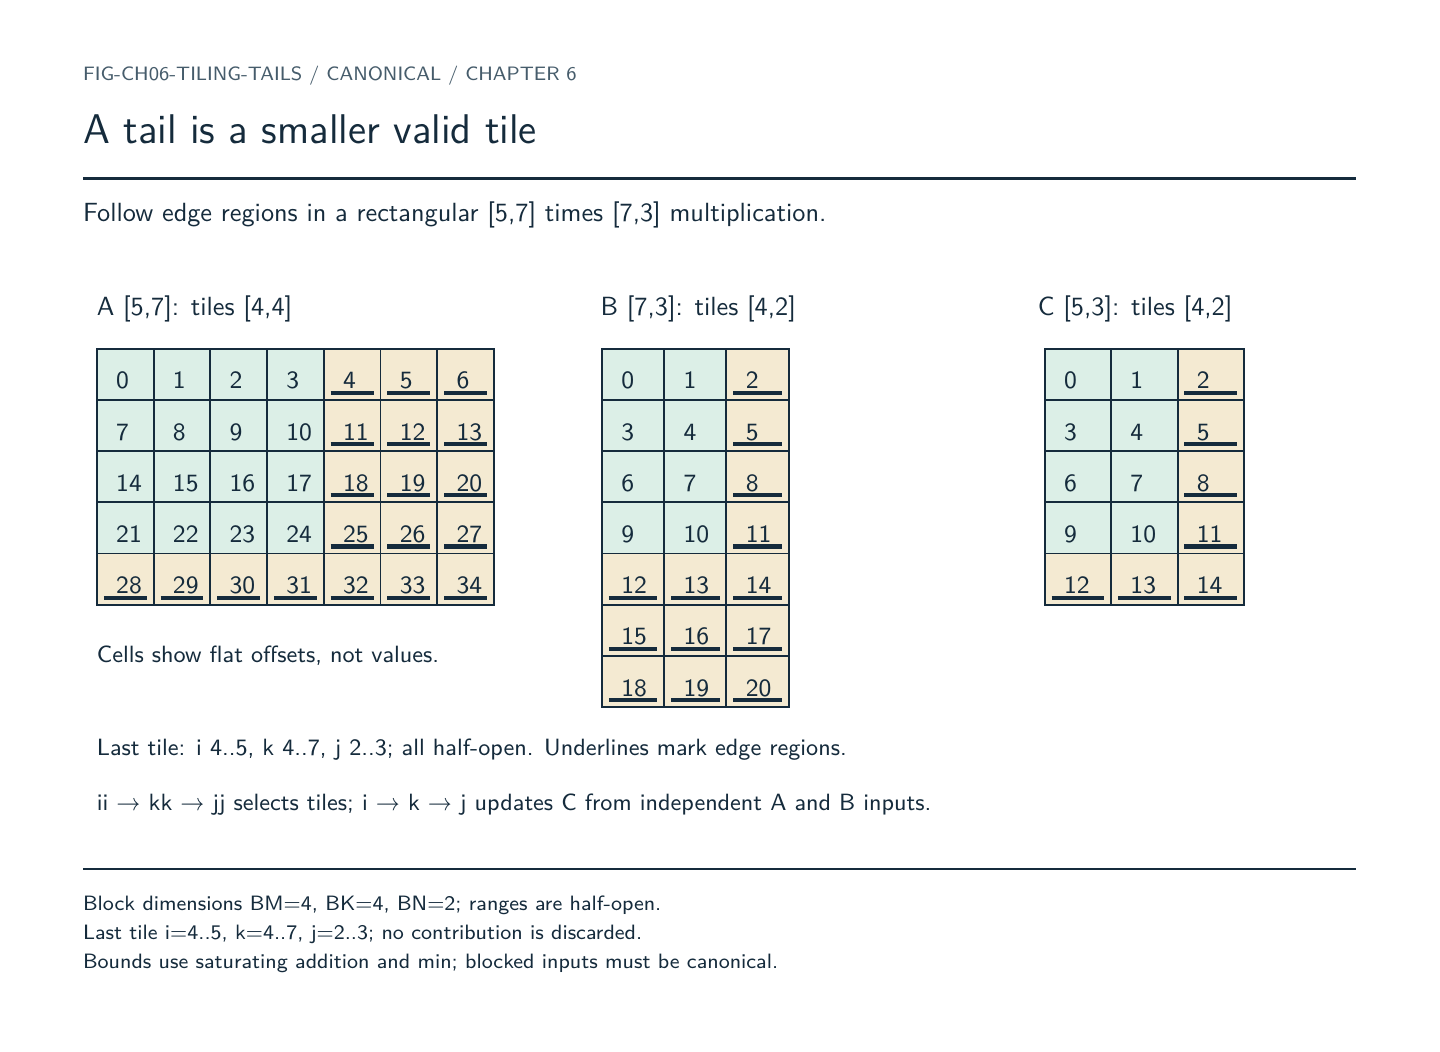
\begin{tikzpicture}[x=.5pt,y=-.5pt]
\path[use as bounding box] (0,0) rectangle (1000,720);
\path[fill=white,draw=none,line width=0.5pt] (0.0,0.0) rectangle (1000.0,720.0);
\node[inner sep=0pt,outer sep=0pt,anchor=base west,text={rgb,255:red,70;green,92;blue,107},font=\sffamily\fontsize{7.0}{8.4}\selectfont] at (40,38) {FIG-CH06-TILING-TAILS  /  CANONICAL / CHAPTER 6};
\node[inner sep=0pt,outer sep=0pt,anchor=base west,text={rgb,255:red,21;green,43;blue,60},font=\sffamily\fontsize{15.0}{18.0}\selectfont] at (40,84) {A tail is a smaller valid tile};
\draw[fill=none,draw={rgb,255:red,21;green,43;blue,60},line width=0.75pt] (40,109) -- (960,109);
\node[inner sep=0pt,outer sep=0pt,anchor=base west,text={rgb,255:red,21;green,43;blue,60},font=\sffamily\fontsize{9.5}{11.4}\selectfont] at (40,140) {Follow edge regions in a rectangular [5,7] times [7,3] multiplication.};
\node[inner sep=0pt,outer sep=0pt,anchor=base west,text={rgb,255:red,21;green,43;blue,60},font=\sffamily\fontsize{9.5}{11.4}\selectfont] at (50,208) {A [5,7]: tiles [4,4]};
\path[fill={rgb,255:red,220;green,239;blue,231},draw={rgb,255:red,21;green,43;blue,60},line width=0.7pt] (50.0,232.0) rectangle (91.0,269.0);
\node[inner sep=0pt,outer sep=0pt,anchor=base west,text={rgb,255:red,21;green,43;blue,60},font=\sffamily\fontsize{9.0}{10.799999999999999}\selectfont] at (64,261) {0};
\path[fill={rgb,255:red,220;green,239;blue,231},draw={rgb,255:red,21;green,43;blue,60},line width=0.7pt] (91.0,232.0) rectangle (132.0,269.0);
\node[inner sep=0pt,outer sep=0pt,anchor=base west,text={rgb,255:red,21;green,43;blue,60},font=\sffamily\fontsize{9.0}{10.799999999999999}\selectfont] at (105,261) {1};
\path[fill={rgb,255:red,220;green,239;blue,231},draw={rgb,255:red,21;green,43;blue,60},line width=0.7pt] (132.0,232.0) rectangle (173.0,269.0);
\node[inner sep=0pt,outer sep=0pt,anchor=base west,text={rgb,255:red,21;green,43;blue,60},font=\sffamily\fontsize{9.0}{10.799999999999999}\selectfont] at (146,261) {2};
\path[fill={rgb,255:red,220;green,239;blue,231},draw={rgb,255:red,21;green,43;blue,60},line width=0.7pt] (173.0,232.0) rectangle (214.0,269.0);
\node[inner sep=0pt,outer sep=0pt,anchor=base west,text={rgb,255:red,21;green,43;blue,60},font=\sffamily\fontsize{9.0}{10.799999999999999}\selectfont] at (187,261) {3};
\path[fill={rgb,255:red,244;green,234;blue,210},draw={rgb,255:red,21;green,43;blue,60},line width=0.7pt] (214.0,232.0) rectangle (255.0,269.0);
\node[inner sep=0pt,outer sep=0pt,anchor=base west,text={rgb,255:red,21;green,43;blue,60},font=\sffamily\fontsize{9.0}{10.799999999999999}\selectfont] at (228,261) {4};
\draw[fill=none,draw={rgb,255:red,21;green,43;blue,60},line width=1.5pt] (219,264) -- (250,264);
\path[fill={rgb,255:red,244;green,234;blue,210},draw={rgb,255:red,21;green,43;blue,60},line width=0.7pt] (255.0,232.0) rectangle (296.0,269.0);
\node[inner sep=0pt,outer sep=0pt,anchor=base west,text={rgb,255:red,21;green,43;blue,60},font=\sffamily\fontsize{9.0}{10.799999999999999}\selectfont] at (269,261) {5};
\draw[fill=none,draw={rgb,255:red,21;green,43;blue,60},line width=1.5pt] (260,264) -- (291,264);
\path[fill={rgb,255:red,244;green,234;blue,210},draw={rgb,255:red,21;green,43;blue,60},line width=0.7pt] (296.0,232.0) rectangle (337.0,269.0);
\node[inner sep=0pt,outer sep=0pt,anchor=base west,text={rgb,255:red,21;green,43;blue,60},font=\sffamily\fontsize{9.0}{10.799999999999999}\selectfont] at (310,261) {6};
\draw[fill=none,draw={rgb,255:red,21;green,43;blue,60},line width=1.5pt] (301,264) -- (332,264);
\path[fill={rgb,255:red,220;green,239;blue,231},draw={rgb,255:red,21;green,43;blue,60},line width=0.7pt] (50.0,269.0) rectangle (91.0,306.0);
\node[inner sep=0pt,outer sep=0pt,anchor=base west,text={rgb,255:red,21;green,43;blue,60},font=\sffamily\fontsize{9.0}{10.799999999999999}\selectfont] at (64,298) {7};
\path[fill={rgb,255:red,220;green,239;blue,231},draw={rgb,255:red,21;green,43;blue,60},line width=0.7pt] (91.0,269.0) rectangle (132.0,306.0);
\node[inner sep=0pt,outer sep=0pt,anchor=base west,text={rgb,255:red,21;green,43;blue,60},font=\sffamily\fontsize{9.0}{10.799999999999999}\selectfont] at (105,298) {8};
\path[fill={rgb,255:red,220;green,239;blue,231},draw={rgb,255:red,21;green,43;blue,60},line width=0.7pt] (132.0,269.0) rectangle (173.0,306.0);
\node[inner sep=0pt,outer sep=0pt,anchor=base west,text={rgb,255:red,21;green,43;blue,60},font=\sffamily\fontsize{9.0}{10.799999999999999}\selectfont] at (146,298) {9};
\path[fill={rgb,255:red,220;green,239;blue,231},draw={rgb,255:red,21;green,43;blue,60},line width=0.7pt] (173.0,269.0) rectangle (214.0,306.0);
\node[inner sep=0pt,outer sep=0pt,anchor=base west,text={rgb,255:red,21;green,43;blue,60},font=\sffamily\fontsize{9.0}{10.799999999999999}\selectfont] at (187,298) {10};
\path[fill={rgb,255:red,244;green,234;blue,210},draw={rgb,255:red,21;green,43;blue,60},line width=0.7pt] (214.0,269.0) rectangle (255.0,306.0);
\node[inner sep=0pt,outer sep=0pt,anchor=base west,text={rgb,255:red,21;green,43;blue,60},font=\sffamily\fontsize{9.0}{10.799999999999999}\selectfont] at (228,298) {11};
\draw[fill=none,draw={rgb,255:red,21;green,43;blue,60},line width=1.5pt] (219,301) -- (250,301);
\path[fill={rgb,255:red,244;green,234;blue,210},draw={rgb,255:red,21;green,43;blue,60},line width=0.7pt] (255.0,269.0) rectangle (296.0,306.0);
\node[inner sep=0pt,outer sep=0pt,anchor=base west,text={rgb,255:red,21;green,43;blue,60},font=\sffamily\fontsize{9.0}{10.799999999999999}\selectfont] at (269,298) {12};
\draw[fill=none,draw={rgb,255:red,21;green,43;blue,60},line width=1.5pt] (260,301) -- (291,301);
\path[fill={rgb,255:red,244;green,234;blue,210},draw={rgb,255:red,21;green,43;blue,60},line width=0.7pt] (296.0,269.0) rectangle (337.0,306.0);
\node[inner sep=0pt,outer sep=0pt,anchor=base west,text={rgb,255:red,21;green,43;blue,60},font=\sffamily\fontsize{9.0}{10.799999999999999}\selectfont] at (310,298) {13};
\draw[fill=none,draw={rgb,255:red,21;green,43;blue,60},line width=1.5pt] (301,301) -- (332,301);
\path[fill={rgb,255:red,220;green,239;blue,231},draw={rgb,255:red,21;green,43;blue,60},line width=0.7pt] (50.0,306.0) rectangle (91.0,343.0);
\node[inner sep=0pt,outer sep=0pt,anchor=base west,text={rgb,255:red,21;green,43;blue,60},font=\sffamily\fontsize{9.0}{10.799999999999999}\selectfont] at (64,335) {14};
\path[fill={rgb,255:red,220;green,239;blue,231},draw={rgb,255:red,21;green,43;blue,60},line width=0.7pt] (91.0,306.0) rectangle (132.0,343.0);
\node[inner sep=0pt,outer sep=0pt,anchor=base west,text={rgb,255:red,21;green,43;blue,60},font=\sffamily\fontsize{9.0}{10.799999999999999}\selectfont] at (105,335) {15};
\path[fill={rgb,255:red,220;green,239;blue,231},draw={rgb,255:red,21;green,43;blue,60},line width=0.7pt] (132.0,306.0) rectangle (173.0,343.0);
\node[inner sep=0pt,outer sep=0pt,anchor=base west,text={rgb,255:red,21;green,43;blue,60},font=\sffamily\fontsize{9.0}{10.799999999999999}\selectfont] at (146,335) {16};
\path[fill={rgb,255:red,220;green,239;blue,231},draw={rgb,255:red,21;green,43;blue,60},line width=0.7pt] (173.0,306.0) rectangle (214.0,343.0);
\node[inner sep=0pt,outer sep=0pt,anchor=base west,text={rgb,255:red,21;green,43;blue,60},font=\sffamily\fontsize{9.0}{10.799999999999999}\selectfont] at (187,335) {17};
\path[fill={rgb,255:red,244;green,234;blue,210},draw={rgb,255:red,21;green,43;blue,60},line width=0.7pt] (214.0,306.0) rectangle (255.0,343.0);
\node[inner sep=0pt,outer sep=0pt,anchor=base west,text={rgb,255:red,21;green,43;blue,60},font=\sffamily\fontsize{9.0}{10.799999999999999}\selectfont] at (228,335) {18};
\draw[fill=none,draw={rgb,255:red,21;green,43;blue,60},line width=1.5pt] (219,338) -- (250,338);
\path[fill={rgb,255:red,244;green,234;blue,210},draw={rgb,255:red,21;green,43;blue,60},line width=0.7pt] (255.0,306.0) rectangle (296.0,343.0);
\node[inner sep=0pt,outer sep=0pt,anchor=base west,text={rgb,255:red,21;green,43;blue,60},font=\sffamily\fontsize{9.0}{10.799999999999999}\selectfont] at (269,335) {19};
\draw[fill=none,draw={rgb,255:red,21;green,43;blue,60},line width=1.5pt] (260,338) -- (291,338);
\path[fill={rgb,255:red,244;green,234;blue,210},draw={rgb,255:red,21;green,43;blue,60},line width=0.7pt] (296.0,306.0) rectangle (337.0,343.0);
\node[inner sep=0pt,outer sep=0pt,anchor=base west,text={rgb,255:red,21;green,43;blue,60},font=\sffamily\fontsize{9.0}{10.799999999999999}\selectfont] at (310,335) {20};
\draw[fill=none,draw={rgb,255:red,21;green,43;blue,60},line width=1.5pt] (301,338) -- (332,338);
\path[fill={rgb,255:red,220;green,239;blue,231},draw={rgb,255:red,21;green,43;blue,60},line width=0.7pt] (50.0,343.0) rectangle (91.0,380.0);
\node[inner sep=0pt,outer sep=0pt,anchor=base west,text={rgb,255:red,21;green,43;blue,60},font=\sffamily\fontsize{9.0}{10.799999999999999}\selectfont] at (64,372) {21};
\path[fill={rgb,255:red,220;green,239;blue,231},draw={rgb,255:red,21;green,43;blue,60},line width=0.7pt] (91.0,343.0) rectangle (132.0,380.0);
\node[inner sep=0pt,outer sep=0pt,anchor=base west,text={rgb,255:red,21;green,43;blue,60},font=\sffamily\fontsize{9.0}{10.799999999999999}\selectfont] at (105,372) {22};
\path[fill={rgb,255:red,220;green,239;blue,231},draw={rgb,255:red,21;green,43;blue,60},line width=0.7pt] (132.0,343.0) rectangle (173.0,380.0);
\node[inner sep=0pt,outer sep=0pt,anchor=base west,text={rgb,255:red,21;green,43;blue,60},font=\sffamily\fontsize{9.0}{10.799999999999999}\selectfont] at (146,372) {23};
\path[fill={rgb,255:red,220;green,239;blue,231},draw={rgb,255:red,21;green,43;blue,60},line width=0.7pt] (173.0,343.0) rectangle (214.0,380.0);
\node[inner sep=0pt,outer sep=0pt,anchor=base west,text={rgb,255:red,21;green,43;blue,60},font=\sffamily\fontsize{9.0}{10.799999999999999}\selectfont] at (187,372) {24};
\path[fill={rgb,255:red,244;green,234;blue,210},draw={rgb,255:red,21;green,43;blue,60},line width=0.7pt] (214.0,343.0) rectangle (255.0,380.0);
\node[inner sep=0pt,outer sep=0pt,anchor=base west,text={rgb,255:red,21;green,43;blue,60},font=\sffamily\fontsize{9.0}{10.799999999999999}\selectfont] at (228,372) {25};
\draw[fill=none,draw={rgb,255:red,21;green,43;blue,60},line width=1.5pt] (219,375) -- (250,375);
\path[fill={rgb,255:red,244;green,234;blue,210},draw={rgb,255:red,21;green,43;blue,60},line width=0.7pt] (255.0,343.0) rectangle (296.0,380.0);
\node[inner sep=0pt,outer sep=0pt,anchor=base west,text={rgb,255:red,21;green,43;blue,60},font=\sffamily\fontsize{9.0}{10.799999999999999}\selectfont] at (269,372) {26};
\draw[fill=none,draw={rgb,255:red,21;green,43;blue,60},line width=1.5pt] (260,375) -- (291,375);
\path[fill={rgb,255:red,244;green,234;blue,210},draw={rgb,255:red,21;green,43;blue,60},line width=0.7pt] (296.0,343.0) rectangle (337.0,380.0);
\node[inner sep=0pt,outer sep=0pt,anchor=base west,text={rgb,255:red,21;green,43;blue,60},font=\sffamily\fontsize{9.0}{10.799999999999999}\selectfont] at (310,372) {27};
\draw[fill=none,draw={rgb,255:red,21;green,43;blue,60},line width=1.5pt] (301,375) -- (332,375);
\path[fill={rgb,255:red,244;green,234;blue,210},draw={rgb,255:red,21;green,43;blue,60},line width=0.7pt] (50.0,380.0) rectangle (91.0,417.0);
\node[inner sep=0pt,outer sep=0pt,anchor=base west,text={rgb,255:red,21;green,43;blue,60},font=\sffamily\fontsize{9.0}{10.799999999999999}\selectfont] at (64,409) {28};
\draw[fill=none,draw={rgb,255:red,21;green,43;blue,60},line width=1.5pt] (55,412) -- (86,412);
\path[fill={rgb,255:red,244;green,234;blue,210},draw={rgb,255:red,21;green,43;blue,60},line width=0.7pt] (91.0,380.0) rectangle (132.0,417.0);
\node[inner sep=0pt,outer sep=0pt,anchor=base west,text={rgb,255:red,21;green,43;blue,60},font=\sffamily\fontsize{9.0}{10.799999999999999}\selectfont] at (105,409) {29};
\draw[fill=none,draw={rgb,255:red,21;green,43;blue,60},line width=1.5pt] (96,412) -- (127,412);
\path[fill={rgb,255:red,244;green,234;blue,210},draw={rgb,255:red,21;green,43;blue,60},line width=0.7pt] (132.0,380.0) rectangle (173.0,417.0);
\node[inner sep=0pt,outer sep=0pt,anchor=base west,text={rgb,255:red,21;green,43;blue,60},font=\sffamily\fontsize{9.0}{10.799999999999999}\selectfont] at (146,409) {30};
\draw[fill=none,draw={rgb,255:red,21;green,43;blue,60},line width=1.5pt] (137,412) -- (168,412);
\path[fill={rgb,255:red,244;green,234;blue,210},draw={rgb,255:red,21;green,43;blue,60},line width=0.7pt] (173.0,380.0) rectangle (214.0,417.0);
\node[inner sep=0pt,outer sep=0pt,anchor=base west,text={rgb,255:red,21;green,43;blue,60},font=\sffamily\fontsize{9.0}{10.799999999999999}\selectfont] at (187,409) {31};
\draw[fill=none,draw={rgb,255:red,21;green,43;blue,60},line width=1.5pt] (178,412) -- (209,412);
\path[fill={rgb,255:red,244;green,234;blue,210},draw={rgb,255:red,21;green,43;blue,60},line width=0.7pt] (214.0,380.0) rectangle (255.0,417.0);
\node[inner sep=0pt,outer sep=0pt,anchor=base west,text={rgb,255:red,21;green,43;blue,60},font=\sffamily\fontsize{9.0}{10.799999999999999}\selectfont] at (228,409) {32};
\draw[fill=none,draw={rgb,255:red,21;green,43;blue,60},line width=1.5pt] (219,412) -- (250,412);
\path[fill={rgb,255:red,244;green,234;blue,210},draw={rgb,255:red,21;green,43;blue,60},line width=0.7pt] (255.0,380.0) rectangle (296.0,417.0);
\node[inner sep=0pt,outer sep=0pt,anchor=base west,text={rgb,255:red,21;green,43;blue,60},font=\sffamily\fontsize{9.0}{10.799999999999999}\selectfont] at (269,409) {33};
\draw[fill=none,draw={rgb,255:red,21;green,43;blue,60},line width=1.5pt] (260,412) -- (291,412);
\path[fill={rgb,255:red,244;green,234;blue,210},draw={rgb,255:red,21;green,43;blue,60},line width=0.7pt] (296.0,380.0) rectangle (337.0,417.0);
\node[inner sep=0pt,outer sep=0pt,anchor=base west,text={rgb,255:red,21;green,43;blue,60},font=\sffamily\fontsize{9.0}{10.799999999999999}\selectfont] at (310,409) {34};
\draw[fill=none,draw={rgb,255:red,21;green,43;blue,60},line width=1.5pt] (301,412) -- (332,412);
\node[inner sep=0pt,outer sep=0pt,anchor=base west,text={rgb,255:red,21;green,43;blue,60},font=\sffamily\fontsize{9.5}{11.4}\selectfont] at (414,208) {B [7,3]: tiles [4,2]};
\path[fill={rgb,255:red,220;green,239;blue,231},draw={rgb,255:red,21;green,43;blue,60},line width=0.7pt] (415.0,232.0) rectangle (460.0,269.0);
\node[inner sep=0pt,outer sep=0pt,anchor=base west,text={rgb,255:red,21;green,43;blue,60},font=\sffamily\fontsize{9.0}{10.799999999999999}\selectfont] at (429,261) {0};
\path[fill={rgb,255:red,220;green,239;blue,231},draw={rgb,255:red,21;green,43;blue,60},line width=0.7pt] (460.0,232.0) rectangle (505.0,269.0);
\node[inner sep=0pt,outer sep=0pt,anchor=base west,text={rgb,255:red,21;green,43;blue,60},font=\sffamily\fontsize{9.0}{10.799999999999999}\selectfont] at (474,261) {1};
\path[fill={rgb,255:red,244;green,234;blue,210},draw={rgb,255:red,21;green,43;blue,60},line width=0.7pt] (505.0,232.0) rectangle (550.0,269.0);
\node[inner sep=0pt,outer sep=0pt,anchor=base west,text={rgb,255:red,21;green,43;blue,60},font=\sffamily\fontsize{9.0}{10.799999999999999}\selectfont] at (519,261) {2};
\draw[fill=none,draw={rgb,255:red,21;green,43;blue,60},line width=1.5pt] (510,264) -- (545,264);
\path[fill={rgb,255:red,220;green,239;blue,231},draw={rgb,255:red,21;green,43;blue,60},line width=0.7pt] (415.0,269.0) rectangle (460.0,306.0);
\node[inner sep=0pt,outer sep=0pt,anchor=base west,text={rgb,255:red,21;green,43;blue,60},font=\sffamily\fontsize{9.0}{10.799999999999999}\selectfont] at (429,298) {3};
\path[fill={rgb,255:red,220;green,239;blue,231},draw={rgb,255:red,21;green,43;blue,60},line width=0.7pt] (460.0,269.0) rectangle (505.0,306.0);
\node[inner sep=0pt,outer sep=0pt,anchor=base west,text={rgb,255:red,21;green,43;blue,60},font=\sffamily\fontsize{9.0}{10.799999999999999}\selectfont] at (474,298) {4};
\path[fill={rgb,255:red,244;green,234;blue,210},draw={rgb,255:red,21;green,43;blue,60},line width=0.7pt] (505.0,269.0) rectangle (550.0,306.0);
\node[inner sep=0pt,outer sep=0pt,anchor=base west,text={rgb,255:red,21;green,43;blue,60},font=\sffamily\fontsize{9.0}{10.799999999999999}\selectfont] at (519,298) {5};
\draw[fill=none,draw={rgb,255:red,21;green,43;blue,60},line width=1.5pt] (510,301) -- (545,301);
\path[fill={rgb,255:red,220;green,239;blue,231},draw={rgb,255:red,21;green,43;blue,60},line width=0.7pt] (415.0,306.0) rectangle (460.0,343.0);
\node[inner sep=0pt,outer sep=0pt,anchor=base west,text={rgb,255:red,21;green,43;blue,60},font=\sffamily\fontsize{9.0}{10.799999999999999}\selectfont] at (429,335) {6};
\path[fill={rgb,255:red,220;green,239;blue,231},draw={rgb,255:red,21;green,43;blue,60},line width=0.7pt] (460.0,306.0) rectangle (505.0,343.0);
\node[inner sep=0pt,outer sep=0pt,anchor=base west,text={rgb,255:red,21;green,43;blue,60},font=\sffamily\fontsize{9.0}{10.799999999999999}\selectfont] at (474,335) {7};
\path[fill={rgb,255:red,244;green,234;blue,210},draw={rgb,255:red,21;green,43;blue,60},line width=0.7pt] (505.0,306.0) rectangle (550.0,343.0);
\node[inner sep=0pt,outer sep=0pt,anchor=base west,text={rgb,255:red,21;green,43;blue,60},font=\sffamily\fontsize{9.0}{10.799999999999999}\selectfont] at (519,335) {8};
\draw[fill=none,draw={rgb,255:red,21;green,43;blue,60},line width=1.5pt] (510,338) -- (545,338);
\path[fill={rgb,255:red,220;green,239;blue,231},draw={rgb,255:red,21;green,43;blue,60},line width=0.7pt] (415.0,343.0) rectangle (460.0,380.0);
\node[inner sep=0pt,outer sep=0pt,anchor=base west,text={rgb,255:red,21;green,43;blue,60},font=\sffamily\fontsize{9.0}{10.799999999999999}\selectfont] at (429,372) {9};
\path[fill={rgb,255:red,220;green,239;blue,231},draw={rgb,255:red,21;green,43;blue,60},line width=0.7pt] (460.0,343.0) rectangle (505.0,380.0);
\node[inner sep=0pt,outer sep=0pt,anchor=base west,text={rgb,255:red,21;green,43;blue,60},font=\sffamily\fontsize{9.0}{10.799999999999999}\selectfont] at (474,372) {10};
\path[fill={rgb,255:red,244;green,234;blue,210},draw={rgb,255:red,21;green,43;blue,60},line width=0.7pt] (505.0,343.0) rectangle (550.0,380.0);
\node[inner sep=0pt,outer sep=0pt,anchor=base west,text={rgb,255:red,21;green,43;blue,60},font=\sffamily\fontsize{9.0}{10.799999999999999}\selectfont] at (519,372) {11};
\draw[fill=none,draw={rgb,255:red,21;green,43;blue,60},line width=1.5pt] (510,375) -- (545,375);
\path[fill={rgb,255:red,244;green,234;blue,210},draw={rgb,255:red,21;green,43;blue,60},line width=0.7pt] (415.0,380.0) rectangle (460.0,417.0);
\node[inner sep=0pt,outer sep=0pt,anchor=base west,text={rgb,255:red,21;green,43;blue,60},font=\sffamily\fontsize{9.0}{10.799999999999999}\selectfont] at (429,409) {12};
\draw[fill=none,draw={rgb,255:red,21;green,43;blue,60},line width=1.5pt] (420,412) -- (455,412);
\path[fill={rgb,255:red,244;green,234;blue,210},draw={rgb,255:red,21;green,43;blue,60},line width=0.7pt] (460.0,380.0) rectangle (505.0,417.0);
\node[inner sep=0pt,outer sep=0pt,anchor=base west,text={rgb,255:red,21;green,43;blue,60},font=\sffamily\fontsize{9.0}{10.799999999999999}\selectfont] at (474,409) {13};
\draw[fill=none,draw={rgb,255:red,21;green,43;blue,60},line width=1.5pt] (465,412) -- (500,412);
\path[fill={rgb,255:red,244;green,234;blue,210},draw={rgb,255:red,21;green,43;blue,60},line width=0.7pt] (505.0,380.0) rectangle (550.0,417.0);
\node[inner sep=0pt,outer sep=0pt,anchor=base west,text={rgb,255:red,21;green,43;blue,60},font=\sffamily\fontsize{9.0}{10.799999999999999}\selectfont] at (519,409) {14};
\draw[fill=none,draw={rgb,255:red,21;green,43;blue,60},line width=1.5pt] (510,412) -- (545,412);
\path[fill={rgb,255:red,244;green,234;blue,210},draw={rgb,255:red,21;green,43;blue,60},line width=0.7pt] (415.0,417.0) rectangle (460.0,454.0);
\node[inner sep=0pt,outer sep=0pt,anchor=base west,text={rgb,255:red,21;green,43;blue,60},font=\sffamily\fontsize{9.0}{10.799999999999999}\selectfont] at (429,446) {15};
\draw[fill=none,draw={rgb,255:red,21;green,43;blue,60},line width=1.5pt] (420,449) -- (455,449);
\path[fill={rgb,255:red,244;green,234;blue,210},draw={rgb,255:red,21;green,43;blue,60},line width=0.7pt] (460.0,417.0) rectangle (505.0,454.0);
\node[inner sep=0pt,outer sep=0pt,anchor=base west,text={rgb,255:red,21;green,43;blue,60},font=\sffamily\fontsize{9.0}{10.799999999999999}\selectfont] at (474,446) {16};
\draw[fill=none,draw={rgb,255:red,21;green,43;blue,60},line width=1.5pt] (465,449) -- (500,449);
\path[fill={rgb,255:red,244;green,234;blue,210},draw={rgb,255:red,21;green,43;blue,60},line width=0.7pt] (505.0,417.0) rectangle (550.0,454.0);
\node[inner sep=0pt,outer sep=0pt,anchor=base west,text={rgb,255:red,21;green,43;blue,60},font=\sffamily\fontsize{9.0}{10.799999999999999}\selectfont] at (519,446) {17};
\draw[fill=none,draw={rgb,255:red,21;green,43;blue,60},line width=1.5pt] (510,449) -- (545,449);
\path[fill={rgb,255:red,244;green,234;blue,210},draw={rgb,255:red,21;green,43;blue,60},line width=0.7pt] (415.0,454.0) rectangle (460.0,491.0);
\node[inner sep=0pt,outer sep=0pt,anchor=base west,text={rgb,255:red,21;green,43;blue,60},font=\sffamily\fontsize{9.0}{10.799999999999999}\selectfont] at (429,483) {18};
\draw[fill=none,draw={rgb,255:red,21;green,43;blue,60},line width=1.5pt] (420,486) -- (455,486);
\path[fill={rgb,255:red,244;green,234;blue,210},draw={rgb,255:red,21;green,43;blue,60},line width=0.7pt] (460.0,454.0) rectangle (505.0,491.0);
\node[inner sep=0pt,outer sep=0pt,anchor=base west,text={rgb,255:red,21;green,43;blue,60},font=\sffamily\fontsize{9.0}{10.799999999999999}\selectfont] at (474,483) {19};
\draw[fill=none,draw={rgb,255:red,21;green,43;blue,60},line width=1.5pt] (465,486) -- (500,486);
\path[fill={rgb,255:red,244;green,234;blue,210},draw={rgb,255:red,21;green,43;blue,60},line width=0.7pt] (505.0,454.0) rectangle (550.0,491.0);
\node[inner sep=0pt,outer sep=0pt,anchor=base west,text={rgb,255:red,21;green,43;blue,60},font=\sffamily\fontsize{9.0}{10.799999999999999}\selectfont] at (519,483) {20};
\draw[fill=none,draw={rgb,255:red,21;green,43;blue,60},line width=1.5pt] (510,486) -- (545,486);
\node[inner sep=0pt,outer sep=0pt,anchor=base west,text={rgb,255:red,21;green,43;blue,60},font=\sffamily\fontsize{9.5}{11.4}\selectfont] at (730,208) {C [5,3]: tiles [4,2]};
\path[fill={rgb,255:red,220;green,239;blue,231},draw={rgb,255:red,21;green,43;blue,60},line width=0.7pt] (735.0,232.0) rectangle (783.0,269.0);
\node[inner sep=0pt,outer sep=0pt,anchor=base west,text={rgb,255:red,21;green,43;blue,60},font=\sffamily\fontsize{9.0}{10.799999999999999}\selectfont] at (749,261) {0};
\path[fill={rgb,255:red,220;green,239;blue,231},draw={rgb,255:red,21;green,43;blue,60},line width=0.7pt] (783.0,232.0) rectangle (831.0,269.0);
\node[inner sep=0pt,outer sep=0pt,anchor=base west,text={rgb,255:red,21;green,43;blue,60},font=\sffamily\fontsize{9.0}{10.799999999999999}\selectfont] at (797,261) {1};
\path[fill={rgb,255:red,244;green,234;blue,210},draw={rgb,255:red,21;green,43;blue,60},line width=0.7pt] (831.0,232.0) rectangle (879.0,269.0);
\node[inner sep=0pt,outer sep=0pt,anchor=base west,text={rgb,255:red,21;green,43;blue,60},font=\sffamily\fontsize{9.0}{10.799999999999999}\selectfont] at (845,261) {2};
\draw[fill=none,draw={rgb,255:red,21;green,43;blue,60},line width=1.5pt] (836,264) -- (874,264);
\path[fill={rgb,255:red,220;green,239;blue,231},draw={rgb,255:red,21;green,43;blue,60},line width=0.7pt] (735.0,269.0) rectangle (783.0,306.0);
\node[inner sep=0pt,outer sep=0pt,anchor=base west,text={rgb,255:red,21;green,43;blue,60},font=\sffamily\fontsize{9.0}{10.799999999999999}\selectfont] at (749,298) {3};
\path[fill={rgb,255:red,220;green,239;blue,231},draw={rgb,255:red,21;green,43;blue,60},line width=0.7pt] (783.0,269.0) rectangle (831.0,306.0);
\node[inner sep=0pt,outer sep=0pt,anchor=base west,text={rgb,255:red,21;green,43;blue,60},font=\sffamily\fontsize{9.0}{10.799999999999999}\selectfont] at (797,298) {4};
\path[fill={rgb,255:red,244;green,234;blue,210},draw={rgb,255:red,21;green,43;blue,60},line width=0.7pt] (831.0,269.0) rectangle (879.0,306.0);
\node[inner sep=0pt,outer sep=0pt,anchor=base west,text={rgb,255:red,21;green,43;blue,60},font=\sffamily\fontsize{9.0}{10.799999999999999}\selectfont] at (845,298) {5};
\draw[fill=none,draw={rgb,255:red,21;green,43;blue,60},line width=1.5pt] (836,301) -- (874,301);
\path[fill={rgb,255:red,220;green,239;blue,231},draw={rgb,255:red,21;green,43;blue,60},line width=0.7pt] (735.0,306.0) rectangle (783.0,343.0);
\node[inner sep=0pt,outer sep=0pt,anchor=base west,text={rgb,255:red,21;green,43;blue,60},font=\sffamily\fontsize{9.0}{10.799999999999999}\selectfont] at (749,335) {6};
\path[fill={rgb,255:red,220;green,239;blue,231},draw={rgb,255:red,21;green,43;blue,60},line width=0.7pt] (783.0,306.0) rectangle (831.0,343.0);
\node[inner sep=0pt,outer sep=0pt,anchor=base west,text={rgb,255:red,21;green,43;blue,60},font=\sffamily\fontsize{9.0}{10.799999999999999}\selectfont] at (797,335) {7};
\path[fill={rgb,255:red,244;green,234;blue,210},draw={rgb,255:red,21;green,43;blue,60},line width=0.7pt] (831.0,306.0) rectangle (879.0,343.0);
\node[inner sep=0pt,outer sep=0pt,anchor=base west,text={rgb,255:red,21;green,43;blue,60},font=\sffamily\fontsize{9.0}{10.799999999999999}\selectfont] at (845,335) {8};
\draw[fill=none,draw={rgb,255:red,21;green,43;blue,60},line width=1.5pt] (836,338) -- (874,338);
\path[fill={rgb,255:red,220;green,239;blue,231},draw={rgb,255:red,21;green,43;blue,60},line width=0.7pt] (735.0,343.0) rectangle (783.0,380.0);
\node[inner sep=0pt,outer sep=0pt,anchor=base west,text={rgb,255:red,21;green,43;blue,60},font=\sffamily\fontsize{9.0}{10.799999999999999}\selectfont] at (749,372) {9};
\path[fill={rgb,255:red,220;green,239;blue,231},draw={rgb,255:red,21;green,43;blue,60},line width=0.7pt] (783.0,343.0) rectangle (831.0,380.0);
\node[inner sep=0pt,outer sep=0pt,anchor=base west,text={rgb,255:red,21;green,43;blue,60},font=\sffamily\fontsize{9.0}{10.799999999999999}\selectfont] at (797,372) {10};
\path[fill={rgb,255:red,244;green,234;blue,210},draw={rgb,255:red,21;green,43;blue,60},line width=0.7pt] (831.0,343.0) rectangle (879.0,380.0);
\node[inner sep=0pt,outer sep=0pt,anchor=base west,text={rgb,255:red,21;green,43;blue,60},font=\sffamily\fontsize{9.0}{10.799999999999999}\selectfont] at (845,372) {11};
\draw[fill=none,draw={rgb,255:red,21;green,43;blue,60},line width=1.5pt] (836,375) -- (874,375);
\path[fill={rgb,255:red,244;green,234;blue,210},draw={rgb,255:red,21;green,43;blue,60},line width=0.7pt] (735.0,380.0) rectangle (783.0,417.0);
\node[inner sep=0pt,outer sep=0pt,anchor=base west,text={rgb,255:red,21;green,43;blue,60},font=\sffamily\fontsize{9.0}{10.799999999999999}\selectfont] at (749,409) {12};
\draw[fill=none,draw={rgb,255:red,21;green,43;blue,60},line width=1.5pt] (740,412) -- (778,412);
\path[fill={rgb,255:red,244;green,234;blue,210},draw={rgb,255:red,21;green,43;blue,60},line width=0.7pt] (783.0,380.0) rectangle (831.0,417.0);
\node[inner sep=0pt,outer sep=0pt,anchor=base west,text={rgb,255:red,21;green,43;blue,60},font=\sffamily\fontsize{9.0}{10.799999999999999}\selectfont] at (797,409) {13};
\draw[fill=none,draw={rgb,255:red,21;green,43;blue,60},line width=1.5pt] (788,412) -- (826,412);
\path[fill={rgb,255:red,244;green,234;blue,210},draw={rgb,255:red,21;green,43;blue,60},line width=0.7pt] (831.0,380.0) rectangle (879.0,417.0);
\node[inner sep=0pt,outer sep=0pt,anchor=base west,text={rgb,255:red,21;green,43;blue,60},font=\sffamily\fontsize{9.0}{10.799999999999999}\selectfont] at (845,409) {14};
\draw[fill=none,draw={rgb,255:red,21;green,43;blue,60},line width=1.5pt] (836,412) -- (874,412);
\node[inner sep=0pt,outer sep=0pt,anchor=base west,text={rgb,255:red,21;green,43;blue,60},font=\sffamily\fontsize{8.5}{10.2}\selectfont] at (50,459) {Cells show flat offsets, not values.};
\node[inner sep=0pt,outer sep=0pt,anchor=base west,text={rgb,255:red,21;green,43;blue,60},font=\sffamily\fontsize{8.5}{10.2}\selectfont] at (50,526) {Last tile: i 4..5, k 4..7, j 2..3; all half-open. Underlines mark edge regions.};
\node[inner sep=0pt,outer sep=0pt,anchor=base west,text={rgb,255:red,21;green,43;blue,60},font=\sffamily\fontsize{8.5}{10.2}\selectfont] at (50,566) {ii → kk → jj selects tiles; i → k → j updates C from independent A and B inputs.};
\draw[fill=none,draw={rgb,255:red,21;green,43;blue,60},line width=0.75pt] (40,608) -- (960,608);
\node[inner sep=0pt,outer sep=0pt,anchor=base west,text={rgb,255:red,21;green,43;blue,60},font=\sffamily\fontsize{7.5}{9.0}\selectfont] at (40,638) {Block dimensions BM=4, BK=4, BN=2; ranges are half-open.};
\node[inner sep=0pt,outer sep=0pt,anchor=base west,text={rgb,255:red,21;green,43;blue,60},font=\sffamily\fontsize{7.5}{9.0}\selectfont] at (40,659) {Last tile i=4..5, k=4..7, j=2..3; no contribution is discarded.};
\node[inner sep=0pt,outer sep=0pt,anchor=base west,text={rgb,255:red,21;green,43;blue,60},font=\sffamily\fontsize{7.5}{9.0}\selectfont] at (40,680) {Bounds use saturating addition and min; blocked inputs must be canonical.};
\end{tikzpicture}
}\caption{Rectangular tile offsets and clipped edge regions in a five-by-seven times seven-by-three product.}\end{figure}

The tail fixture deliberately uses a different shape from the small
numerical spine: \texttt{{[}5,7{]}\ ×\ {[}7,3{]}} with blocks
\texttt{{[}4,4,2{]}}. The last tile covers \texttt{i=4..5},
\texttt{k=4..7}, \texttt{j=2..3}, all half-open. Its three scalar
contributions are as real as those in a full tile. There are eight tile
combinations; clipping bounds avoids padding requirements and dropping
remainders. The test compares every output against the general
reference. Tile diagrams show flat offsets here, not invented matrix
values.

The blocked kernel does not call checked multidimensional indexing for
each multiply. It validates rank, inner dimensions, output size, block
size, and layout once.
\texttt{\seqsplit{TensorView::as\_contiguous\_slice}} then returns the
exact logical range only when strides equal canonical row-major strides.
Inside the loop, flat indices operate on safe Rust slices.

This is not the removal of safety. It is the movement of repeated
validation to a boundary whose proof applies to the whole loop. The
crate retains \texttt{\seqsplit{\#![forbid(unsafe\_code)]}}; slice
indexing remains bounds checked by Rust, and shape construction has
already proved representable storage extents.

Reference and blocked policies are intentionally different:

\Needspace{14\baselineskip}

{\def\LTcaptype{none} % do not increment counter
\begin{longtable}[]{@{}
  >{\raggedright\arraybackslash}p{(\linewidth - 4\tabcolsep) * \real{0.3333}}
  >{\raggedright\arraybackslash}p{(\linewidth - 4\tabcolsep) * \real{0.3333}}
  >{\raggedright\arraybackslash}p{(\linewidth - 4\tabcolsep) * \real{0.3333}}@{}}
\toprule\noalign{}
\begin{minipage}[b]{\linewidth}\raggedright
Property
\end{minipage} & \begin{minipage}[b]{\linewidth}\raggedright
Reference
\end{minipage} & \begin{minipage}[b]{\linewidth}\raggedright
Blocked
\end{minipage} \\
\midrule\noalign{}
\endhead
\bottomrule\noalign{}
\endlastfoot
Accepted rank & matrices only & matrices only \\
Valid layouts & any checked read-only strides & strict canonical
row-major \\
Inner order & \texttt{i,j,k} & tiled \texttt{i,k,j} \\
Input mutation & never & never \\
Output & new canonical owner & new canonical owner \\
Hidden materialization & never & never \\
\end{longtable}
}

The
\href{https://github.com/hermonai/inside-the-llm-engine/blob/astra-visual-rewrite/diagrams/linear/reference-vs-blocked-kernel.txt}{kernel-contract
diagram} captures the boundary. If a caller wants to multiply a
transpose view with the blocked path, it must call
\texttt{to\_contiguous()} explicitly. The copy is then visible in code,
cost accounting, and ownership.

\begin{quote}
\textbf{ENGINEERING FAILURE --- THE INVISIBLE COPY} An optimized API
receives a strided transpose, silently packs it, runs a fast kernel, and
reports only kernel time. The result is correct but the system paid
allocation and copy costs that its call site cannot see. ENGINE-2
returns \texttt{\seqsplit{UnsupportedLayout}} instead.
\end{quote}

\subsection{Reference versus
optimized}\label{reference-versus-optimized}

An optimized substitution is valid only if it preserves the selected
contract. It need not preserve internal iteration order. For each
accepted input it must produce the same output shape and numerically
equivalent values, leave inputs unchanged, return independent owned
storage, handle empty dimensions, and return documented errors before
invalid execution.

Keeping the reference path makes those claims testable. It also leaves a
fallback for valid strided views and a small implementation that
reviewers can compare directly with the equation. Production libraries
keep analogous fallbacks and differential oracles because optimized code
has more edge paths, not fewer.

The
\href{https://github.com/hermonai/inside-the-llm-engine/blob/astra-visual-rewrite/diagrams/linear/optimization-ladder.txt}{optimization
ladder} places blocking in context. Packing, register blocking, SIMD
microkernels, threading, NUMA placement, accelerators, and fusion remain
later rungs. ENGINE-2 stops at scalar cache blocking so the first
optimization remains inspectable. The
\href{https://github.com/hermonai/inside-the-llm-engine/blob/astra-visual-rewrite/diagrams/linear/reference-candidate-gates.txt}{reference/candidate
gate} states the contract, equivalence, and performance-evidence
sequence required before a candidate can replace the oracle path.

\subsection{Prove it: independent
oracle}\label{prove-it-independent-oracle}

\texttt{\seqsplit{code/reference/python/chapter06\_matmul\_oracle.py}}
imports no Rust or mini-engine code. It implements dot, GEMV, and GEMM
with Python lists and uses \texttt{struct.pack}/\texttt{unpack} to round
each multiplication and addition to binary32. Its fixtures include:

\begin{itemize}
\tightlist
\item
  the exact dot result 12 for \texttt{{[}1,2,3{]}\ ·\ {[}4,-5,6{]}};
\item
  the asymmetric GEMV result \texttt{{[}1.5,6{]}};
\item
  the complete hand GEMM result \texttt{\seqsplit{[[58,64],[139,154]]}};
\item
  fractional values and negative terms;
\item
  a logical transpose product;
\item
  the empty-dot identity.
\end{itemize}

An independent oracle can share a mistaken specification, but it is less
likely to share the same indexing defect than a second call through the
Rust kernel. Hand expansion supplies another line of evidence.

\subsection{Prove it: equivalence gate}\label{prove-it-equivalence-gate}

ENGINE-2 uses

\[
|a-r|\le \epsilon_{abs}+\epsilon_{rel}|r|,
\]

with \(\epsilon_{abs}=10^{-5}\) and \(\epsilon_{rel}=10^{-5}\) for
chapter fixtures. Absolute tolerance protects values near zero; relative
tolerance scales with result magnitude. The tolerance is narrow enough
for these bounded fixtures and is not declared universal for arbitrary
reduction lengths or value distributions.

The deterministic property-style test spans every \(M,K,N\) from 0
through 6 and three distinct block shapes. It includes empty products,
tiny matrices, exact tiles, and tails without introducing a random-test
dependency. Additional tests cover strided reference inputs, zero-stride
views, invalid ranks, mismatched inner dimensions, non-canonical blocked
operands, zero block dimensions, output overflow, and independent output
ownership.

\subsection{Floating-point order is
observable}\label{floating-point-order-is-observable}

Real-number addition is associative:

\[
(a+b)+c=a+(b+c).
\]

Finite floating-point addition need not be. Rounding after an
intermediate sum can discard information that a different grouping
preserves. A simple reduction order is therefore part of a
reproducibility story even when it is not part of the abstract linear
algebra.

An executable binary32 example uses \(a=2^{24}\), \(b=1\),
\(c=-2^{24}\):

\[
\operatorname{fl}(\operatorname{fl}(a+b)+c)=0,
\qquad
\operatorname{fl}(a+\operatorname{fl}(b+c))=1.
\]

At that positive magnitude, the first grouping loses the unit before
cancellation; the second preserves it. The new test evaluates both
groupings as \texttt{f32}, with black-box inputs. This is rounding, not
an indexing defect.

Fusing also changes the rounding points. Set \(u=1+2^{-13}\) and
\(v=1-2^{-13}\). Both are exactly representable binary32 inputs. Their
exact product is \(1-2^{-26}\), which rounds to 1 when stored as F32:

\[
\operatorname{fl}(\operatorname{fl}(uv)-1)=0,
\qquad \operatorname{fma}(u,v,-1)=-2^{-26}.
\]

The test uses explicit \texttt{mul\_add} only to demonstrate this
distinction. The teaching kernels do not call it. A vector reduction may
create several partial sums and combine them later, adding another
reason to state numerical policy separately from the real-number
equation.

The reference kernel visits K in ascending order for each cell. The
blocked kernel visits K tiles in ascending order and K within each tile
in ascending order. Its interleaving across different output cells
changes, but the sequence of contributions to an individual cell remains
ordered. That makes the current paths especially close. The API still
specifies tolerance rather than bitwise equivalence because compiler
contraction, target instructions, and future legal kernel
transformations can affect rounding.

Using \texttt{f64} accumulation would reduce error for many \texttt{f32}
inputs, but it would also define a different kernel cost and numerical
contract. ENGINE-2 chooses \texttt{f32} input, accumulator, and output
because it keeps the scalar teaching path aligned with its stored dtype.
The choice is explicit, not asserted optimal. Later low-precision or
quantized kernels will have to state storage, product, and accumulator
types separately.

NaN and infinity policy also deserves precision. Model construction
rejects non-finite parameters, and \texttt{Logits} rejects non-finite
results. The generic linear kernels themselves perform ordinary
\texttt{f32} arithmetic and do not scan all inputs for finiteness. That
keeps them mathematical primitives rather than silently embedding the
model's parameter policy. A caller that needs a finite- input contract
must validate at its own boundary.

Determinism is correspondingly bounded. For the same build, target,
inputs, and selected scalar path, iteration order is fixed. ENGINE-2
does not promise bit-identical output across all compilers and
architectures. It promises shape and ownership semantics plus numerical
equivalence under the documented test tolerance.

\begin{quote}
\textbf{PROVE IT} Run
\href{https://github.com/hermonai/inside-the-llm-engine/blob/astra-visual-rewrite/labs/lab-28-kernel-equivalence.md}{Lab
28}. Record maximum error; never widen a tolerance until the discrepancy
has an explanation.
\end{quote}

Floating-point tolerance cannot excuse a structural bug. A wrong offset
may occasionally produce a close number. That is why shape checks, exact
integer fixtures, full-output comparisons, tails, and error variants
surround the numerical metric.

\subsection{Performance lab: blocking}\label{performance-lab-blocking}

The blocked benchmark sweeps cubic tile sizes 8, 16, 24, 32, 48, and 64
at shape \texttt{192³}. On the recorded Apple M1 run, tile 64 had the
lowest median among those candidates, while tile 8 was slower than the
direct \texttt{ijk} control. The teaching default of 32 was not the
measured winner.

A second experiment held the 32 tile fixed and varied square size:

{\def\LTcaptype{none} % do not increment counter
\begin{longtable}[]{@{}
  >{\raggedleft\arraybackslash}p{(\linewidth - 6\tabcolsep) * \real{0.2500}}
  >{\raggedleft\arraybackslash}p{(\linewidth - 6\tabcolsep) * \real{0.2500}}
  >{\raggedleft\arraybackslash}p{(\linewidth - 6\tabcolsep) * \real{0.2500}}
  >{\raggedleft\arraybackslash}p{(\linewidth - 6\tabcolsep) * \real{0.2500}}@{}}
\toprule\noalign{}
\begin{minipage}[b]{\linewidth}\raggedleft
Size
\end{minipage} & \begin{minipage}[b]{\linewidth}\raggedleft
Direct \texttt{ijk}
\end{minipage} & \begin{minipage}[b]{\linewidth}\raggedleft
Blocked 32
\end{minipage} & \begin{minipage}[b]{\linewidth}\raggedleft
Speedup: direct time / blocked time
\end{minipage} \\
\midrule\noalign{}
\endhead
\bottomrule\noalign{}
\endlastfoot
8 & 333 ns & 1,000 ns & 0.33× \\
16 & 2,459 ns & 2,834 ns & 0.87× \\
32 & 19,375 ns & 12,500 ns & 1.55× \\
64 & 178,333 ns & 93,125 ns & 1.91× \\
128 & 1,668,500 ns & 755,625 ns & 2.21× \\
\end{longtable}
}

\begin{figure}[H]\centering\resizebox{\linewidth}{!}{% Generated from figures/generated/ch06-crossover.svg; do not hand edit.
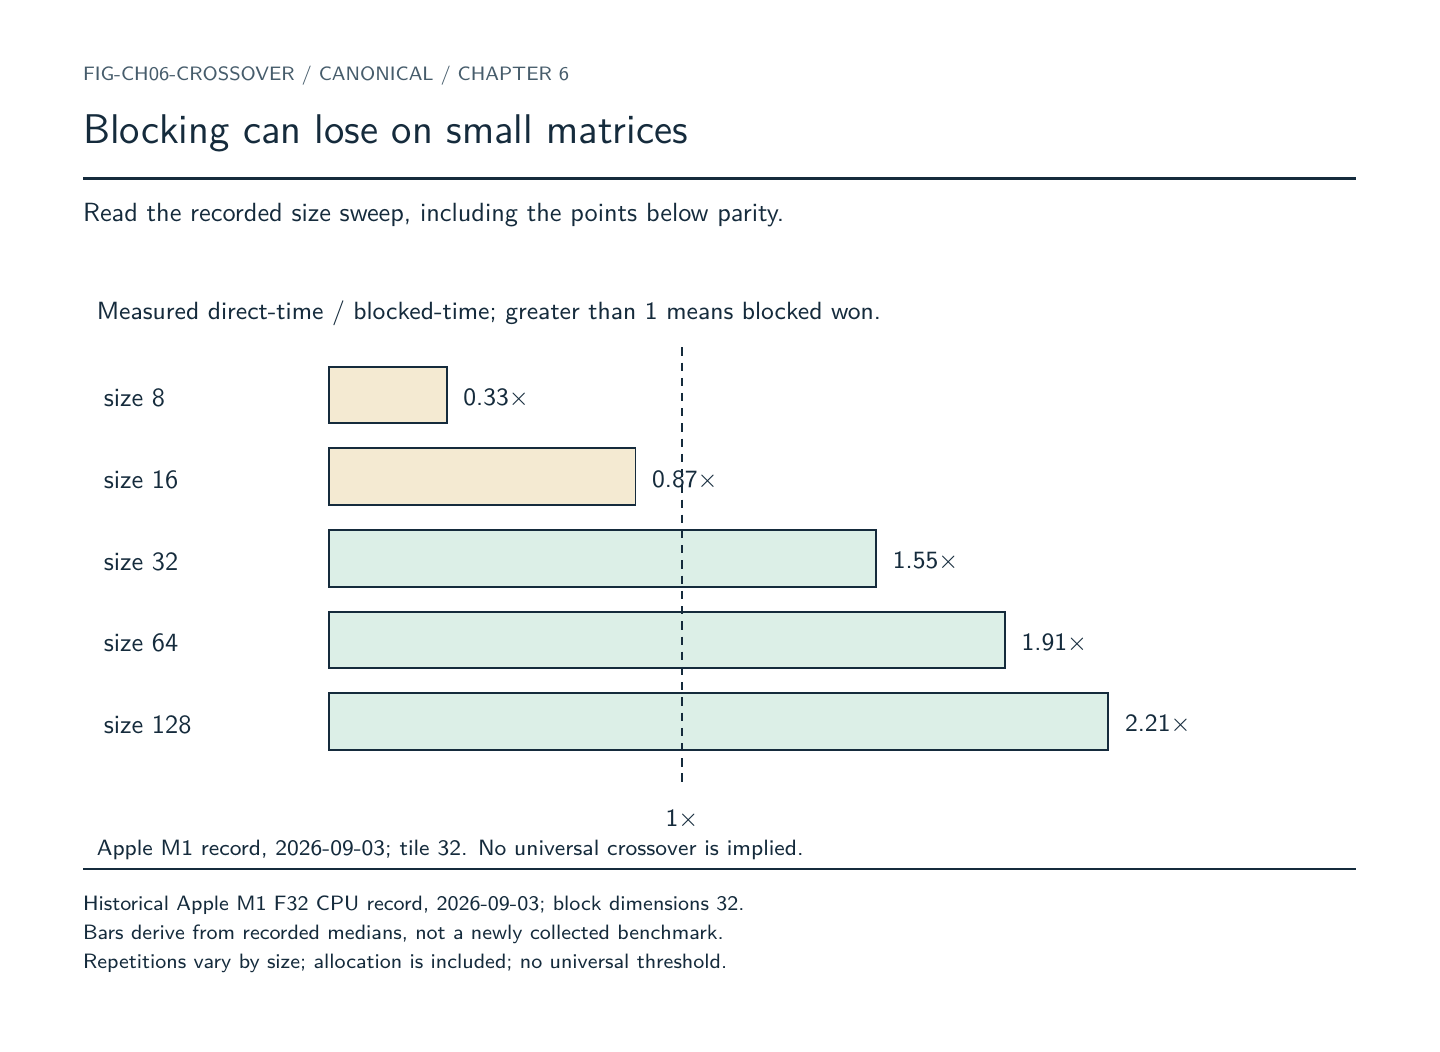
\begin{tikzpicture}[x=.5pt,y=-.5pt]
\path[use as bounding box] (0,0) rectangle (1000,720);
\path[fill=white,draw=none,line width=0.5pt] (0.0,0.0) rectangle (1000.0,720.0);
\node[inner sep=0pt,outer sep=0pt,anchor=base west,text={rgb,255:red,70;green,92;blue,107},font=\sffamily\fontsize{7.0}{8.4}\selectfont] at (40,38) {FIG-CH06-CROSSOVER  /  CANONICAL / CHAPTER 6};
\node[inner sep=0pt,outer sep=0pt,anchor=base west,text={rgb,255:red,21;green,43;blue,60},font=\sffamily\fontsize{15.0}{18.0}\selectfont] at (40,84) {Blocking can lose on small matrices};
\draw[fill=none,draw={rgb,255:red,21;green,43;blue,60},line width=0.75pt] (40,109) -- (960,109);
\node[inner sep=0pt,outer sep=0pt,anchor=base west,text={rgb,255:red,21;green,43;blue,60},font=\sffamily\fontsize{9.5}{11.4}\selectfont] at (40,140) {Read the recorded size sweep, including the points below parity.};
\node[inner sep=0pt,outer sep=0pt,anchor=base west,text={rgb,255:red,21;green,43;blue,60},font=\sffamily\fontsize{9.0}{10.799999999999999}\selectfont] at (50,211) {Measured direct-time / blocked-time; greater than 1 means blocked won.};
\node[inner sep=0pt,outer sep=0pt,anchor=base west,text={rgb,255:red,21;green,43;blue,60},font=\sffamily\fontsize{9.5}{11.4}\selectfont] at (55,274) {size 8};
\path[fill={rgb,255:red,244;green,234;blue,210},draw={rgb,255:red,21;green,43;blue,60},line width=0.7pt] (218.0,245.0) rectangle (302.915,286.0);
\node[inner sep=0pt,outer sep=0pt,anchor=base west,text={rgb,255:red,21;green,43;blue,60},font=\sffamily\fontsize{9.5}{11.4}\selectfont] at (232,274) {};
\node[inner sep=0pt,outer sep=0pt,anchor=base west,text={rgb,255:red,21;green,43;blue,60},font=\sffamily\fontsize{9.0}{10.799999999999999}\selectfont] at (314.915,273) {0.33×};
\node[inner sep=0pt,outer sep=0pt,anchor=base west,text={rgb,255:red,21;green,43;blue,60},font=\sffamily\fontsize{9.5}{11.4}\selectfont] at (55,333) {size 16};
\path[fill={rgb,255:red,244;green,234;blue,210},draw={rgb,255:red,21;green,43;blue,60},line width=0.7pt] (218.0,304.0) rectangle (439.257939308398,345.0);
\node[inner sep=0pt,outer sep=0pt,anchor=base west,text={rgb,255:red,21;green,43;blue,60},font=\sffamily\fontsize{9.5}{11.4}\selectfont] at (232,333) {};
\node[inner sep=0pt,outer sep=0pt,anchor=base west,text={rgb,255:red,21;green,43;blue,60},font=\sffamily\fontsize{9.0}{10.799999999999999}\selectfont] at (451.257939308398,332) {0.87×};
\node[inner sep=0pt,outer sep=0pt,anchor=base west,text={rgb,255:red,21;green,43;blue,60},font=\sffamily\fontsize{9.5}{11.4}\selectfont] at (55,392) {size 32};
\path[fill={rgb,255:red,220;green,239;blue,231},draw={rgb,255:red,21;green,43;blue,60},line width=0.7pt] (218.0,363.0) rectangle (613.25,404.0);
\node[inner sep=0pt,outer sep=0pt,anchor=base west,text={rgb,255:red,21;green,43;blue,60},font=\sffamily\fontsize{9.5}{11.4}\selectfont] at (232,392) {};
\node[inner sep=0pt,outer sep=0pt,anchor=base west,text={rgb,255:red,21;green,43;blue,60},font=\sffamily\fontsize{9.0}{10.799999999999999}\selectfont] at (625.25,391) {1.55×};
\node[inner sep=0pt,outer sep=0pt,anchor=base west,text={rgb,255:red,21;green,43;blue,60},font=\sffamily\fontsize{9.5}{11.4}\selectfont] at (55,451) {size 64};
\path[fill={rgb,255:red,220;green,239;blue,231},draw={rgb,255:red,21;green,43;blue,60},line width=0.7pt] (218.0,422.0) rectangle (706.3212348993288,463.0);
\node[inner sep=0pt,outer sep=0pt,anchor=base west,text={rgb,255:red,21;green,43;blue,60},font=\sffamily\fontsize{9.5}{11.4}\selectfont] at (232,451) {};
\node[inner sep=0pt,outer sep=0pt,anchor=base west,text={rgb,255:red,21;green,43;blue,60},font=\sffamily\fontsize{9.0}{10.799999999999999}\selectfont] at (718.3212348993288,450) {1.91×};
\node[inner sep=0pt,outer sep=0pt,anchor=base west,text={rgb,255:red,21;green,43;blue,60},font=\sffamily\fontsize{9.5}{11.4}\selectfont] at (55,510) {size 128};
\path[fill={rgb,255:red,220;green,239;blue,231},draw={rgb,255:red,21;green,43;blue,60},line width=0.7pt] (218.0,481.0) rectangle (781.0669975186104,522.0);
\node[inner sep=0pt,outer sep=0pt,anchor=base west,text={rgb,255:red,21;green,43;blue,60},font=\sffamily\fontsize{9.5}{11.4}\selectfont] at (232,510) {};
\node[inner sep=0pt,outer sep=0pt,anchor=base west,text={rgb,255:red,21;green,43;blue,60},font=\sffamily\fontsize{9.0}{10.799999999999999}\selectfont] at (793.0669975186104,509) {2.21×};
\draw[fill=none,draw={rgb,255:red,21;green,43;blue,60},line width=0.75pt,dash pattern=on 3.0pt off 2.5pt] (473,231) -- (473,548);
\node[inner sep=0pt,outer sep=0pt,anchor=base west,text={rgb,255:red,21;green,43;blue,60},font=\sffamily\fontsize{9.0}{10.799999999999999}\selectfont] at (461,577) {1×};
\node[inner sep=0pt,outer sep=0pt,anchor=base west,text={rgb,255:red,21;green,43;blue,60},font=\sffamily\fontsize{8.0}{9.6}\selectfont] at (50,598) {Apple M1 record, 2026-09-03; tile 32. No universal crossover is implied.};
\draw[fill=none,draw={rgb,255:red,21;green,43;blue,60},line width=0.75pt] (40,608) -- (960,608);
\node[inner sep=0pt,outer sep=0pt,anchor=base west,text={rgb,255:red,21;green,43;blue,60},font=\sffamily\fontsize{7.5}{9.0}\selectfont] at (40,638) {Historical Apple M1 F32 CPU record, 2026-09-03; block dimensions 32.};
\node[inner sep=0pt,outer sep=0pt,anchor=base west,text={rgb,255:red,21;green,43;blue,60},font=\sffamily\fontsize{7.5}{9.0}\selectfont] at (40,659) {Bars derive from recorded medians, not a newly collected benchmark.};
\node[inner sep=0pt,outer sep=0pt,anchor=base west,text={rgb,255:red,21;green,43;blue,60},font=\sffamily\fontsize{7.5}{9.0}\selectfont] at (40,680) {Repetitions vary by size; allocation is included; no universal threshold.};
\end{tikzpicture}
}\caption{Historical direct-time over blocked-time ratios retain the two losses below parity.}\end{figure}

For sizes 8 and 16, the blocked call lost on this run. Extra
tile/control work is a plausible explanation, but no experiment isolated
that cause. Blocking began winning somewhere between the tested sizes 16
and 32; that bracket is workload- and machine-specific. See the
\href{https://github.com/hermonai/inside-the-llm-engine/blob/astra-visual-rewrite/research/benchmarks/chapter-06-blocked-matmul.md}{blocked-matmul
record} for raw results and full limitations.

This is what an honest optimization result looks like: it contains
losing cases. ``Blocked'' is not a synonym for ``fast.'' Optimization
has a workload.

\subsection{Performance lab: GEMV versus
GEMM}\label{performance-lab-gemv-versus-gemm}

The third experiment holds a \texttt{{[}512,512{]}} weight matrix
constant while changing the right-hand column count. One column uses
scalar GEMV; 8 and 64 columns use blocked GEMM.

{\def\LTcaptype{none} % do not increment counter
\begin{longtable}[]{@{}rlrrr@{}}
\toprule\noalign{}
Columns \(N\) & Kernel & Median & Effective GFLOP/s & Ideal FLOP/byte \\
\midrule\noalign{}
\endhead
\bottomrule\noalign{}
\endlastfoot
1 & GEMV & 191,416 ns & 2.739 & 0.498 \\
8 & blocked GEMM & 3,294,459 ns & 1.273 & 3.879 \\
64 & blocked GEMM & 6,217,167 ns & 5.397 & 25.600 \\
\end{longtable}
}

\begin{figure}[H]\centering\resizebox{\linewidth}{!}{% Generated from figures/generated/ch06-throughput.svg; do not hand edit.
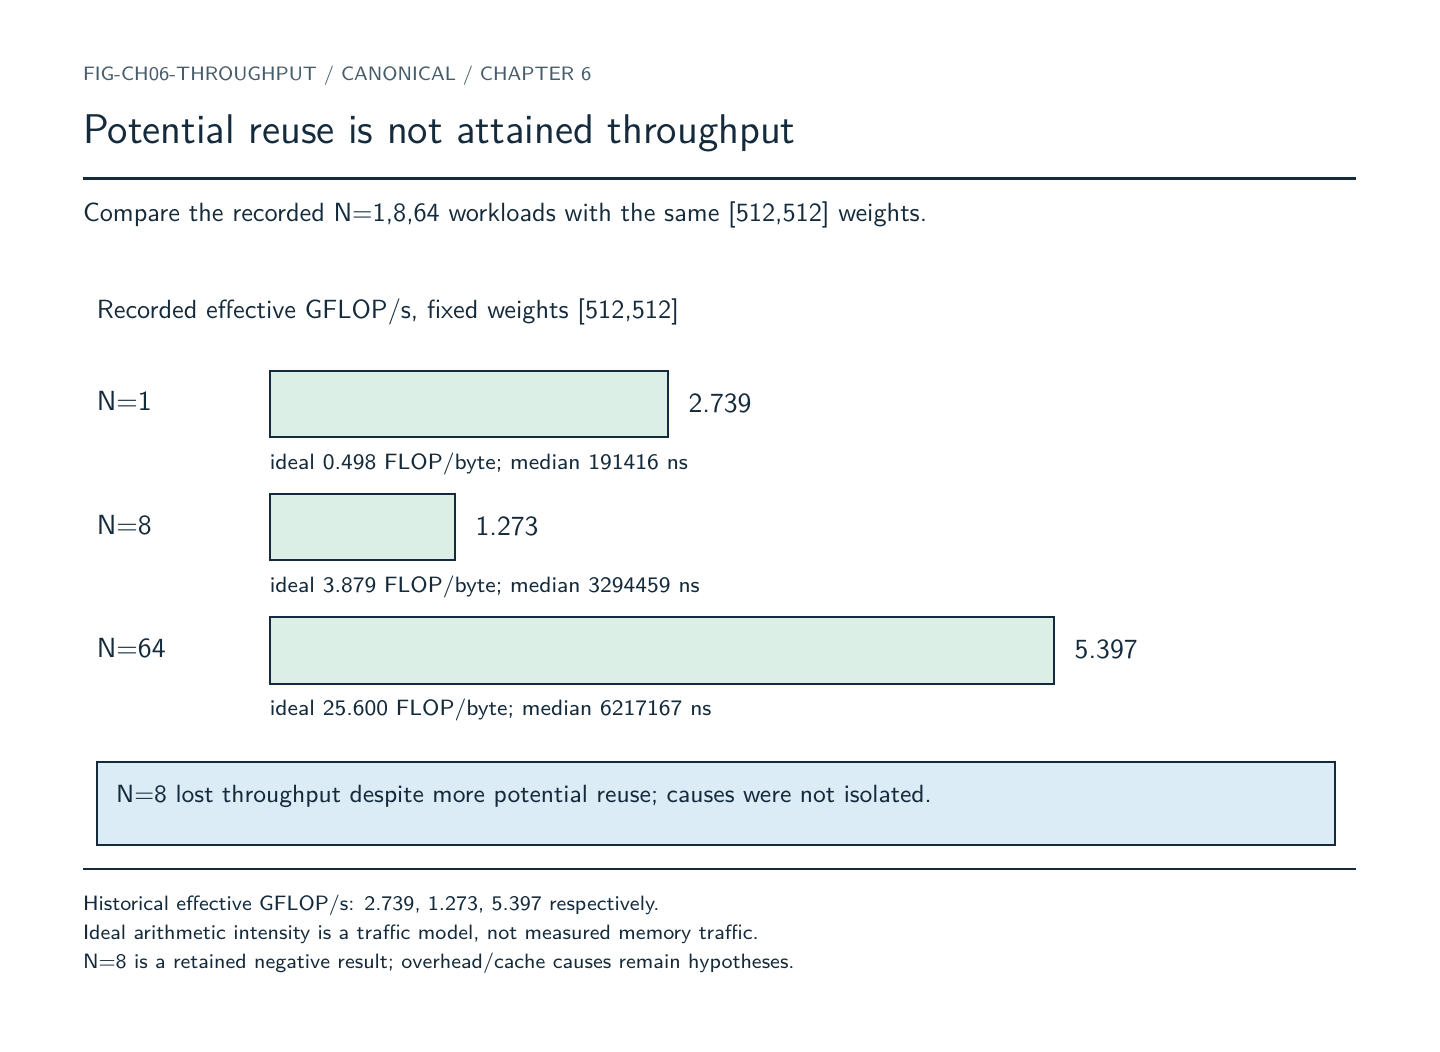
\begin{tikzpicture}[x=.5pt,y=-.5pt]
\path[use as bounding box] (0,0) rectangle (1000,720);
\path[fill=white,draw=none,line width=0.5pt] (0.0,0.0) rectangle (1000.0,720.0);
\node[inner sep=0pt,outer sep=0pt,anchor=base west,text={rgb,255:red,70;green,92;blue,107},font=\sffamily\fontsize{7.0}{8.4}\selectfont] at (40,38) {FIG-CH06-THROUGHPUT  /  CANONICAL / CHAPTER 6};
\node[inner sep=0pt,outer sep=0pt,anchor=base west,text={rgb,255:red,21;green,43;blue,60},font=\sffamily\fontsize{15.0}{18.0}\selectfont] at (40,84) {Potential reuse is not attained throughput};
\draw[fill=none,draw={rgb,255:red,21;green,43;blue,60},line width=0.75pt] (40,109) -- (960,109);
\node[inner sep=0pt,outer sep=0pt,anchor=base west,text={rgb,255:red,21;green,43;blue,60},font=\sffamily\fontsize{9.5}{11.4}\selectfont] at (40,140) {Compare the recorded N=1,8,64 workloads with the same [512,512] weights.};
\node[inner sep=0pt,outer sep=0pt,anchor=base west,text={rgb,255:red,21;green,43;blue,60},font=\sffamily\fontsize{9.5}{11.4}\selectfont] at (50,210) {Recorded effective GFLOP/s, fixed weights [512,512]};
\node[inner sep=0pt,outer sep=0pt,anchor=base west,text={rgb,255:red,21;green,43;blue,60},font=\sffamily\fontsize{10.0}{12.0}\selectfont] at (50,277) {N=1};
\path[fill={rgb,255:red,220;green,239;blue,231},draw={rgb,255:red,21;green,43;blue,60},line width=0.7pt] (175.0,248.0) rectangle (462.59499999999997,296.0);
\node[inner sep=0pt,outer sep=0pt,anchor=base west,text={rgb,255:red,21;green,43;blue,60},font=\sffamily\fontsize{9.5}{11.4}\selectfont] at (189,277) {};
\node[inner sep=0pt,outer sep=0pt,anchor=base west,text={rgb,255:red,21;green,43;blue,60},font=\sffamily\fontsize{10.0}{12.0}\selectfont] at (477.59499999999997,278) {2.739};
\node[inner sep=0pt,outer sep=0pt,anchor=base west,text={rgb,255:red,21;green,43;blue,60},font=\sffamily\fontsize{8.0}{9.6}\selectfont] at (175,319) {ideal 0.498 FLOP/byte; median 191416 ns};
\node[inner sep=0pt,outer sep=0pt,anchor=base west,text={rgb,255:red,21;green,43;blue,60},font=\sffamily\fontsize{10.0}{12.0}\selectfont] at (50,366) {N=8};
\path[fill={rgb,255:red,220;green,239;blue,231},draw={rgb,255:red,21;green,43;blue,60},line width=0.7pt] (175.0,337.0) rectangle (308.66499999999996,385.0);
\node[inner sep=0pt,outer sep=0pt,anchor=base west,text={rgb,255:red,21;green,43;blue,60},font=\sffamily\fontsize{9.5}{11.4}\selectfont] at (189,366) {};
\node[inner sep=0pt,outer sep=0pt,anchor=base west,text={rgb,255:red,21;green,43;blue,60},font=\sffamily\fontsize{10.0}{12.0}\selectfont] at (323.66499999999996,367) {1.273};
\node[inner sep=0pt,outer sep=0pt,anchor=base west,text={rgb,255:red,21;green,43;blue,60},font=\sffamily\fontsize{8.0}{9.6}\selectfont] at (175,408) {ideal 3.879 FLOP/byte; median 3294459 ns};
\node[inner sep=0pt,outer sep=0pt,anchor=base west,text={rgb,255:red,21;green,43;blue,60},font=\sffamily\fontsize{10.0}{12.0}\selectfont] at (50,455) {N=64};
\path[fill={rgb,255:red,220;green,239;blue,231},draw={rgb,255:red,21;green,43;blue,60},line width=0.7pt] (175.0,426.0) rectangle (741.6850000000001,474.0);
\node[inner sep=0pt,outer sep=0pt,anchor=base west,text={rgb,255:red,21;green,43;blue,60},font=\sffamily\fontsize{9.5}{11.4}\selectfont] at (189,455) {};
\node[inner sep=0pt,outer sep=0pt,anchor=base west,text={rgb,255:red,21;green,43;blue,60},font=\sffamily\fontsize{10.0}{12.0}\selectfont] at (756.6850000000001,456) {5.397};
\node[inner sep=0pt,outer sep=0pt,anchor=base west,text={rgb,255:red,21;green,43;blue,60},font=\sffamily\fontsize{8.0}{9.6}\selectfont] at (175,497) {ideal 25.600 FLOP/byte; median 6217167 ns};
\path[fill={rgb,255:red,220;green,236;blue,247},draw={rgb,255:red,21;green,43;blue,60},line width=0.7pt] (50.0,531.0) rectangle (945.0,591.0);
\node[inner sep=0pt,outer sep=0pt,anchor=base west,text={rgb,255:red,21;green,43;blue,60},font=\sffamily\fontsize{9.0}{10.799999999999999}\selectfont] at (64,560) {N=8 lost throughput despite more potential reuse; causes were not isolated.};
\node[inner sep=0pt,outer sep=0pt,anchor=base west,text={rgb,255:red,21;green,43;blue,60},font=\sffamily\fontsize{9.0}{10.799999999999999}\selectfont] at (64,585) {};
\draw[fill=none,draw={rgb,255:red,21;green,43;blue,60},line width=0.75pt] (40,608) -- (960,608);
\node[inner sep=0pt,outer sep=0pt,anchor=base west,text={rgb,255:red,21;green,43;blue,60},font=\sffamily\fontsize{7.5}{9.0}\selectfont] at (40,638) {Historical effective GFLOP/s: 2.739, 1.273, 5.397 respectively.};
\node[inner sep=0pt,outer sep=0pt,anchor=base west,text={rgb,255:red,21;green,43;blue,60},font=\sffamily\fontsize{7.5}{9.0}\selectfont] at (40,659) {Ideal arithmetic intensity is a traffic model, not measured memory traffic.};
\node[inner sep=0pt,outer sep=0pt,anchor=base west,text={rgb,255:red,21;green,43;blue,60},font=\sffamily\fontsize{7.5}{9.0}\selectfont] at (40,680) {N=8 is a retained negative result; overhead/cache causes remain hypotheses.};
\end{tikzpicture}
}\caption{Measured GEMV and blocked GEMM throughput beside separately modeled ideal intensity.}\end{figure}

The analytic reuse opportunity rises monotonically. The observed scalar
rate did not. The narrow \texttt{N=8} blocked workload achieved less
effective throughput than the GEMV case, while \texttt{N=64} exceeded
both. Short inner row segments, tile overhead, and cache behavior are
hypotheses for this untuned kernel, not measured causes. The
\href{https://github.com/hermonai/inside-the-llm-engine/blob/astra-visual-rewrite/research/benchmarks/chapter-06-gemv-vs-gemm.md}{GEMV/GEMM
record} contains the reproducer and caveats; the
\href{https://github.com/hermonai/inside-the-llm-engine/blob/astra-visual-rewrite/diagrams/linear/gemv-vs-gemm-reuse.txt}{reuse
comparison diagram} shows only opportunity, not guaranteed performance.

\begin{quote}
\textbf{PERFORMANCE LAB} In
\href{https://github.com/hermonai/inside-the-llm-engine/blob/astra-visual-rewrite/labs/lab-29-gemv-vs-gemm.md}{Lab
29}, keep total latency, effective throughput, ideal bytes, and measured
bytes conceptually separate.
\end{quote}

\subsection{ENGINE-2: replace the projection
loop}\label{engine-2-replace-the-projection-loop}

All three performance sections above retain the \textbf{2026-09-03
historical record}, pinned to \texttt{03e08a87} (full hash in each
linked record). The regenerated charts parse those records directly.
Running the examples during this edition's verification does not replace
the published medians. The historical benchmark helper accepts
absolute/relative tolerances \texttt{1e-4/1e-5}; the bounded unit
fixtures use \texttt{1e-5/1e-5}. They are deliberately reported as
separate gates. Neither permits NaN to pass by a comparison trick.

The ENGINE-1 model now creates a rank-1 borrowed view over its
request-owned hidden activation and calls

\begin{verbatim}
gemv_reference(&self.output_weight.view(), &hidden_view)
\end{verbatim}

The kernel returns \(W\mathbf{h}\) as a new owned vector. The model then
adds its bias explicitly and constructs finite \texttt{Logits}. The
\href{https://github.com/hermonai/inside-the-llm-engine/blob/astra-visual-rewrite/diagrams/linear/weight-orientation.txt}{weight-orientation
diagram} shows that each \texttt{{[}V,D{]}} row belongs to one candidate
token. No transpose is implied or materialized.

Embedding remains a row lookup:

\[
\mathbf{h}=E[x].
\]

Selecting row \(x\) from \(E:[V,D]\) is not matrix multiplication.
Recasting it as a one-hot GEMV would add \(VD\) mostly useless
arithmetic and obscure the actual operation. Kernel reuse should clarify
the model, not force every operation through one abstraction.

The Chapter 3 fixture remains the numerical regression gate. Input
\texttt{like} still produces logits

\[
[-0.7,\ 0.1,\ 0.4,\ 2.2],
\]

and the autoregressive sequence remains \texttt{Rust} followed by EOS.
This proves that extracting GEMV changed architecture without changing
observable model semantics.

The
\href{https://github.com/hermonai/inside-the-llm-engine/blob/astra-visual-rewrite/diagrams/linear/engine-2-kernel-stack.txt}{ENGINE-2
stack diagram} shows the new boundary. Tensors describe storage; the
\texttt{linear} module performs operators; the model composes an
embedding lookup, GEMV, and bias addition. Putting \texttt{matmul}
methods directly on \texttt{OwnedTensor} would blur those layers and
make policy---reference versus blocked, layout requirements, future
provider selection---look like an intrinsic property of storage.

\subsection{The public kernel
contract}\label{the-public-kernel-contract}

ENGINE-2 exposes four free functions:

\begin{verbatim}
dot_reference(left, right) -> Result<f32, KernelError>
gemv_reference(matrix, vector) -> Result<OwnedTensor, KernelError>
matmul_reference(left, right) -> Result<OwnedTensor, KernelError>
matmul_blocked(left, right, block) -> Result<OwnedTensor, KernelError>
\end{verbatim}

\texttt{KernelError} distinguishes wrong rank, vector length mismatch,
matrix inner dimension mismatch, unsupported optimized layout, invalid
block size, output shape overflow, and lower-level tensor failure. The
error variants preserve operation and operand context where that context
helps diagnosis.

The contract has no output aliasing. Both inputs are immutable views.
Every tensor output is a fresh canonical owner. Reference calls accept
any view whose non-negative strides and extent pass Tensor Substrate v1.
Blocked calls require strict canonical row-major strides, including axes
of length one. Neither path silently changes shape or layout.

\begin{quote}
\textbf{BREAK IT}
\href{https://github.com/hermonai/inside-the-llm-engine/blob/astra-visual-rewrite/labs/lab-27-break-the-kernel.md}{Lab
27} turns every contract clause into a typed failure. A valid transpose
is accepted by reference GEMM and rejected by blocked GEMM until the
caller explicitly materializes it.
\end{quote}

\subsection{Inside Hermon}\label{inside-hermon-2}

Hermon is the book's industrial reference, not the source of ENGINE-2's
API. At freshly inspected commit \texttt{2a3fd521} (full pin in the
source ledger), its safe Rust surface validates matrix/vector and
matrix/matrix dimensions before crossing a foreign-function boundary.
The linked runtime routes packed weights into a native tensor bridge.
That bridge constructs GGML tensors and an operation graph around
\texttt{ggml\_mul\_mat}; a tensor session owns execution state across
the unsafe boundary.

Status matters. Hermon's default execution remains its batched llama.cpp
path. Its Hermon-owned paged path is PREVIEW and gated rather than
silently selected. The \texttt{paged.rs} row-major \texttt{f32}
multiplication is test/oracle support, not proof that the production
runtime uses a Rust scalar GEMM for normal inference. The GGUF packed
path validates layout and shapes before native graph construction.

\begin{quote}
\textbf{INSIDE HERMON --- CURRENT/LIBRARY/PREVIEW} CURRENT Hermon checks
contracts and dispatches its default batched runtime. LIBRARY code in
pinned GGML performs the industrial matrix operation. PREVIEW
Hermon-owned paging remains explicitly gated. These layers must not be
blended into one performance claim.
\end{quote}

The comparison is useful because it exposes how much ENGINE-2 postpones:
packed weight formats, native graph lifetime, backend dispatch,
architecture specialization, threads, and accelerators. It also
validates the architectural lesson that layout and shape checks belong
before the hot native execution boundary.

The current default route is concrete: \texttt{dispatch.rs} selects the
batched runtime; \texttt{batched.rs} calls
\texttt{\seqsplit{Context::decode\_batch}}; \texttt{linked.rs} crosses
\texttt{\seqsplit{hermon\_llama\_decode\_batch}}; \texttt{shim.c}
invokes \texttt{llama\_decode}. The model graph then reaches GGML
operations and configured backends. This is not the same route as the
optional packed tensor bundle API.

For that separate API, \texttt{matvec\_f32} delegates to
\texttt{matmul\_f32} with one input row. The bundle call validates one
through eight weight names, positive input rows, compatible
rank/dimensions and shared width, checked element counts and native
integer conversions. A mutable \texttt{TensorSession} supplies exclusive
access to reusable context/threadpool state. The C++ bridge checks host
weight residency, copies the F32 input into a GGML tensor, creates one
\texttt{ggml\_mul\_mat} node per weight, computes the graph, and copies
results into Rust-owned output vectors. It is a \textbf{host CPU
bridge}, not evidence that this helper dispatches to the default model's
GPU backend. \texttt{paged.rs} uses the bundle interface on the gated
PREVIEW path; library availability alone does not make it the default.

\begin{figure}[H]\centering\resizebox{\linewidth}{!}{% Generated from figures/generated/ch06-source.svg; do not hand edit.
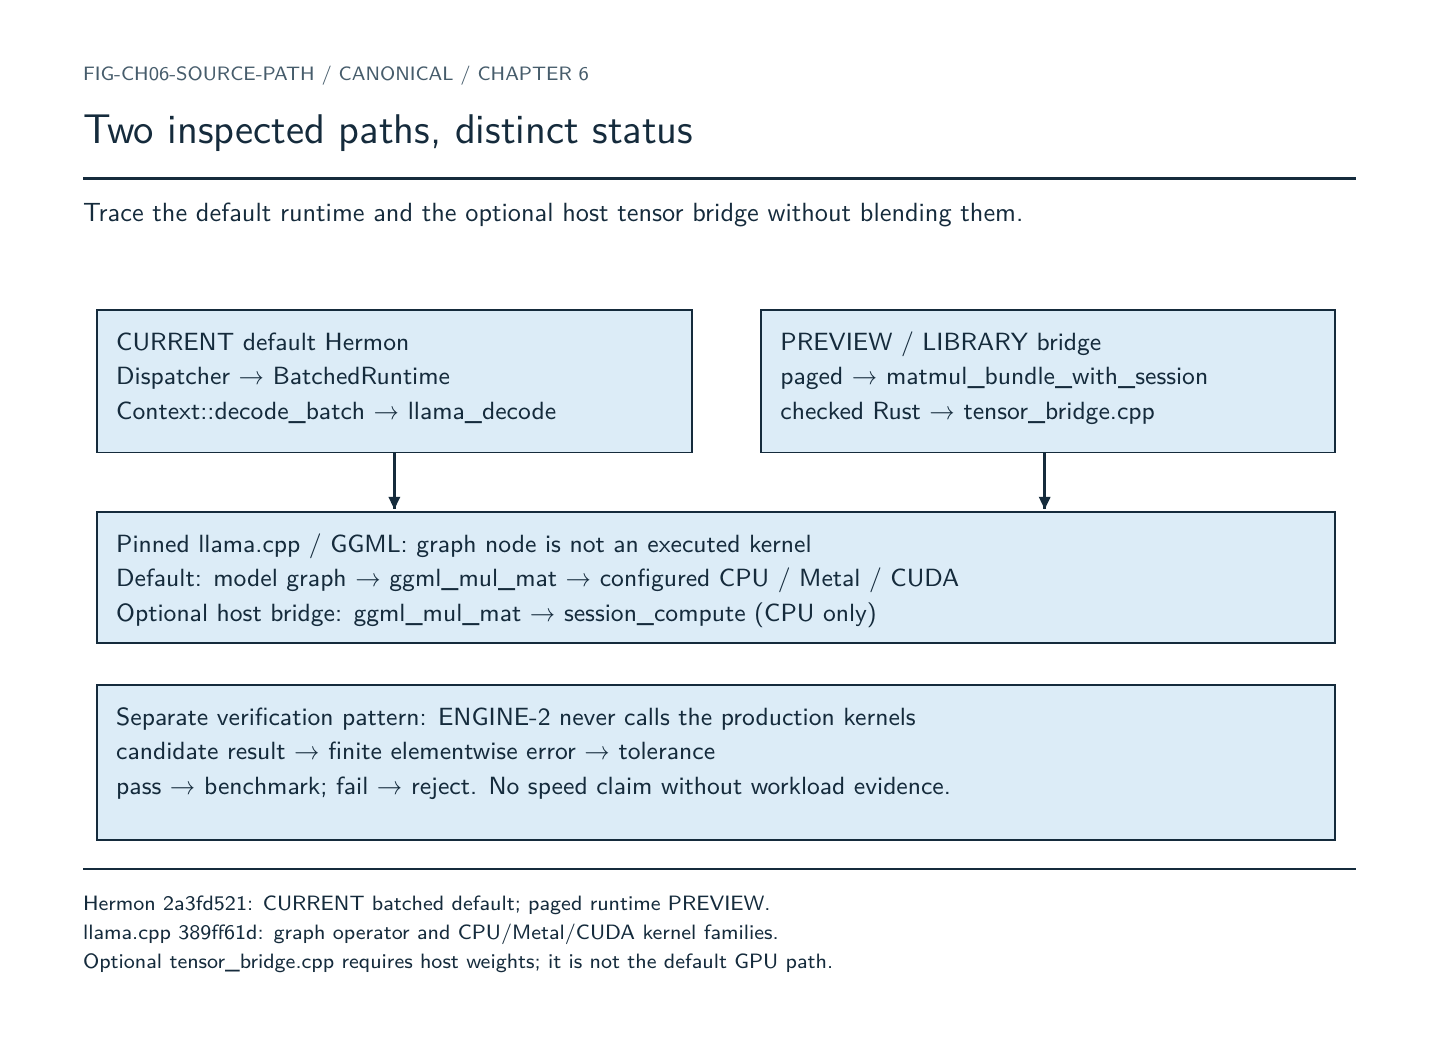
\begin{tikzpicture}[x=.5pt,y=-.5pt]
\path[use as bounding box] (0,0) rectangle (1000,720);
\path[fill=white,draw=none,line width=0.5pt] (0.0,0.0) rectangle (1000.0,720.0);
\node[inner sep=0pt,outer sep=0pt,anchor=base west,text={rgb,255:red,70;green,92;blue,107},font=\sffamily\fontsize{7.0}{8.4}\selectfont] at (40,38) {FIG-CH06-SOURCE-PATH  /  CANONICAL / CHAPTER 6};
\node[inner sep=0pt,outer sep=0pt,anchor=base west,text={rgb,255:red,21;green,43;blue,60},font=\sffamily\fontsize{15.0}{18.0}\selectfont] at (40,84) {Two inspected paths, distinct status};
\draw[fill=none,draw={rgb,255:red,21;green,43;blue,60},line width=0.75pt] (40,109) -- (960,109);
\node[inner sep=0pt,outer sep=0pt,anchor=base west,text={rgb,255:red,21;green,43;blue,60},font=\sffamily\fontsize{9.5}{11.4}\selectfont] at (40,140) {Trace the default runtime and the optional host tensor bridge without blending them.};
\path[fill={rgb,255:red,220;green,236;blue,247},draw={rgb,255:red,21;green,43;blue,60},line width=0.7pt] (50.0,204.0) rectangle (480.0,307.0);
\node[inner sep=0pt,outer sep=0pt,anchor=base west,text={rgb,255:red,21;green,43;blue,60},font=\sffamily\fontsize{9.0}{10.799999999999999}\selectfont] at (64,233) {CURRENT default Hermon};
\node[inner sep=0pt,outer sep=0pt,anchor=base west,text={rgb,255:red,21;green,43;blue,60},font=\sffamily\fontsize{9.0}{10.799999999999999}\selectfont] at (64,258) {Dispatcher → BatchedRuntime};
\node[inner sep=0pt,outer sep=0pt,anchor=base west,text={rgb,255:red,21;green,43;blue,60},font=\sffamily\fontsize{9.0}{10.799999999999999}\selectfont] at (64,283) {Context::decode\_batch → llama\_decode};
\path[fill={rgb,255:red,220;green,236;blue,247},draw={rgb,255:red,21;green,43;blue,60},line width=0.7pt] (530.0,204.0) rectangle (945.0,307.0);
\node[inner sep=0pt,outer sep=0pt,anchor=base west,text={rgb,255:red,21;green,43;blue,60},font=\sffamily\fontsize{9.0}{10.799999999999999}\selectfont] at (544,233) {PREVIEW / LIBRARY bridge};
\node[inner sep=0pt,outer sep=0pt,anchor=base west,text={rgb,255:red,21;green,43;blue,60},font=\sffamily\fontsize{9.0}{10.799999999999999}\selectfont] at (544,258) {paged → matmul\_bundle\_with\_session};
\node[inner sep=0pt,outer sep=0pt,anchor=base west,text={rgb,255:red,21;green,43;blue,60},font=\sffamily\fontsize{9.0}{10.799999999999999}\selectfont] at (544,283) {checked Rust → tensor\_bridge.cpp};
\draw[fill=none,draw={rgb,255:red,21;green,43;blue,60},line width=1.25pt] (265,307) -- (265,348);
\path[fill={rgb,255:red,21;green,43;blue,60},draw=none,line width=0.5pt] (265.00,348.00) -- (260.65,339.00) -- (269.35,339.00) -- cycle;
\draw[fill=none,draw={rgb,255:red,21;green,43;blue,60},line width=1.25pt] (735,307) -- (735,348);
\path[fill={rgb,255:red,21;green,43;blue,60},draw=none,line width=0.5pt] (735.00,348.00) -- (730.65,339.00) -- (739.35,339.00) -- cycle;
\path[fill={rgb,255:red,220;green,236;blue,247},draw={rgb,255:red,21;green,43;blue,60},line width=0.7pt] (50.0,350.0) rectangle (945.0,445.0);
\node[inner sep=0pt,outer sep=0pt,anchor=base west,text={rgb,255:red,21;green,43;blue,60},font=\sffamily\fontsize{9.0}{10.799999999999999}\selectfont] at (64,379) {Pinned llama.cpp / GGML: graph node is not an executed kernel};
\node[inner sep=0pt,outer sep=0pt,anchor=base west,text={rgb,255:red,21;green,43;blue,60},font=\sffamily\fontsize{9.0}{10.799999999999999}\selectfont] at (64,404) {Default: model graph → ggml\_mul\_mat → configured CPU / Metal / CUDA};
\node[inner sep=0pt,outer sep=0pt,anchor=base west,text={rgb,255:red,21;green,43;blue,60},font=\sffamily\fontsize{9.0}{10.799999999999999}\selectfont] at (64,429) {Optional host bridge: ggml\_mul\_mat → session\_compute (CPU only)};
\path[fill={rgb,255:red,220;green,236;blue,247},draw={rgb,255:red,21;green,43;blue,60},line width=0.7pt] (50.0,475.0) rectangle (945.0,587.0);
\node[inner sep=0pt,outer sep=0pt,anchor=base west,text={rgb,255:red,21;green,43;blue,60},font=\sffamily\fontsize{9.0}{10.799999999999999}\selectfont] at (64,504) {Separate verification pattern: ENGINE-2 never calls the production kernels};
\node[inner sep=0pt,outer sep=0pt,anchor=base west,text={rgb,255:red,21;green,43;blue,60},font=\sffamily\fontsize{9.0}{10.799999999999999}\selectfont] at (64,529) {candidate result → finite elementwise error → tolerance};
\node[inner sep=0pt,outer sep=0pt,anchor=base west,text={rgb,255:red,21;green,43;blue,60},font=\sffamily\fontsize{9.0}{10.799999999999999}\selectfont] at (64,554) {pass → benchmark; fail → reject. No speed claim without workload evidence.};
\draw[fill=none,draw={rgb,255:red,21;green,43;blue,60},line width=0.75pt] (40,608) -- (960,608);
\node[inner sep=0pt,outer sep=0pt,anchor=base west,text={rgb,255:red,21;green,43;blue,60},font=\sffamily\fontsize{7.5}{9.0}\selectfont] at (40,638) {Hermon 2a3fd521: CURRENT batched default; paged runtime PREVIEW.};
\node[inner sep=0pt,outer sep=0pt,anchor=base west,text={rgb,255:red,21;green,43;blue,60},font=\sffamily\fontsize{7.5}{9.0}\selectfont] at (40,659) {llama.cpp 389ff61d: graph operator and CPU/Metal/CUDA kernel families.};
\node[inner sep=0pt,outer sep=0pt,anchor=base west,text={rgb,255:red,21;green,43;blue,60},font=\sffamily\fontsize{7.5}{9.0}\selectfont] at (40,680) {Optional tensor\_bridge.cpp requires host weights; it is not the default GPU path.};
\end{tikzpicture}
}\caption{Default batched execution and optional host bridge converge on GGML semantics, with independent ENGINE-2 verification below.}\end{figure}

The
\href{https://github.com/hermonai/inside-the-llm-engine/blob/astra-visual-rewrite/research/astra/chapter06-regeneration.md}{dated
source ledger} records the exact files, symbols, commits, and status of
these findings. Local source inspection establishes available paths and
checks, not a claim that a particular GPU ran a particular request. This
chapter did not launch an industrial model or benchmark Hermon.

\subsection{Inside llama.cpp and GGML}\label{inside-llama.cpp-and-ggml}

Hermon's pinned llama.cpp submodule was inspected at \texttt{389ff61d}
(full pin in the source ledger). GGML's public \texttt{ggml\_mul\_mat}
contract uses its own dimension conventions and supports selected type
pairs. CPU dispatch selects type-specific vector-dot functions. The CPU
kernel examines strides and contiguity, partitions work into
tiles/chunks, and can select architecture-specific implementations;
other backends have separate Metal and CUDA \texttt{MUL\_MAT} paths.

The production lesson is not ``copy GGML into the teaching engine.'' It
is that high-performance multiplication is a family of shape-, type-,
layout-, and hardware-dependent kernels behind a validated contract.
Even names and matrix orientation must be translated carefully at a
boundary. ENGINE-2's
\texttt{{[}M,K{]}\ ×\ {[}K,N{]}\ -\textgreater{}\ {[}M,N{]}} convention
is deliberately explicit so readers do not infer semantics from a
foreign function name.

GGML also demonstrates the optimization rungs beyond this chapter:
type-driven dot kernels, packing assumptions, register-scale work,
parallel scheduling, and accelerator dispatch. Those mechanisms are
real, but introducing them before a scalar oracle would make failures
harder to localize.

\begin{figure}[H]\centering\resizebox{\linewidth}{!}{% Generated from figures/generated/ch06-production.svg; do not hand edit.
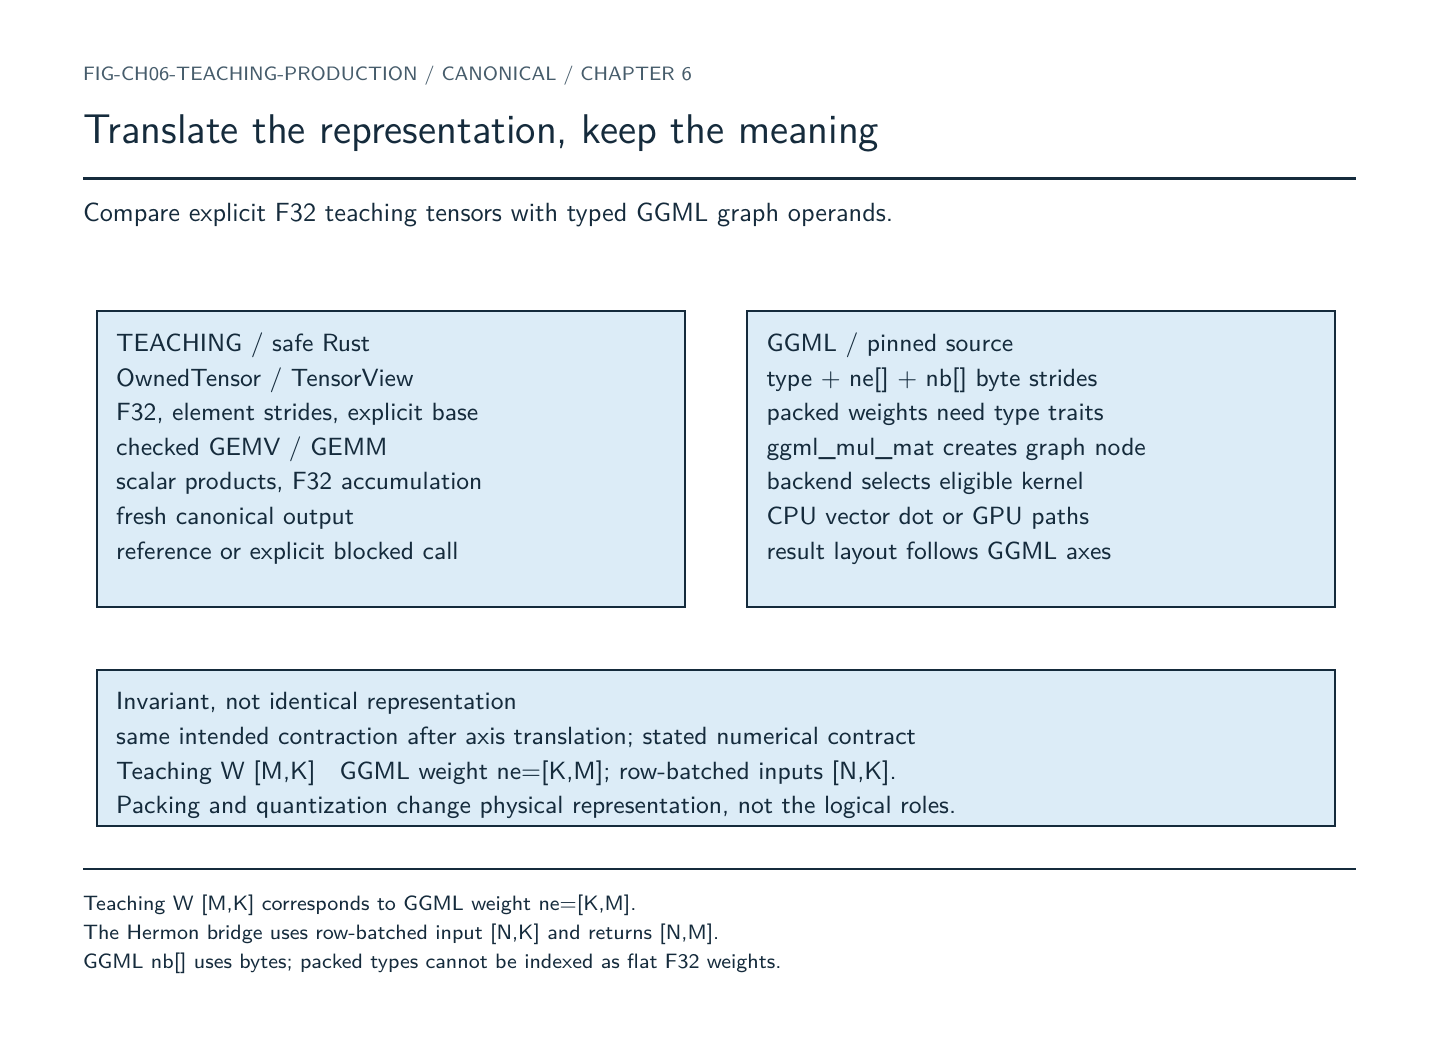
\begin{tikzpicture}[x=.5pt,y=-.5pt]
\path[use as bounding box] (0,0) rectangle (1000,720);
\path[fill=white,draw=none,line width=0.5pt] (0.0,0.0) rectangle (1000.0,720.0);
\node[inner sep=0pt,outer sep=0pt,anchor=base west,text={rgb,255:red,70;green,92;blue,107},font=\sffamily\fontsize{7.0}{8.4}\selectfont] at (40,38) {FIG-CH06-TEACHING-PRODUCTION  /  CANONICAL / CHAPTER 6};
\node[inner sep=0pt,outer sep=0pt,anchor=base west,text={rgb,255:red,21;green,43;blue,60},font=\sffamily\fontsize{15.0}{18.0}\selectfont] at (40,84) {Translate the representation, keep the meaning};
\draw[fill=none,draw={rgb,255:red,21;green,43;blue,60},line width=0.75pt] (40,109) -- (960,109);
\node[inner sep=0pt,outer sep=0pt,anchor=base west,text={rgb,255:red,21;green,43;blue,60},font=\sffamily\fontsize{9.5}{11.4}\selectfont] at (40,140) {Compare explicit F32 teaching tensors with typed GGML graph operands.};
\path[fill={rgb,255:red,220;green,236;blue,247},draw={rgb,255:red,21;green,43;blue,60},line width=0.7pt] (50.0,205.0) rectangle (475.0,419.0);
\node[inner sep=0pt,outer sep=0pt,anchor=base west,text={rgb,255:red,21;green,43;blue,60},font=\sffamily\fontsize{9.0}{10.799999999999999}\selectfont] at (64,234) {TEACHING / safe Rust};
\node[inner sep=0pt,outer sep=0pt,anchor=base west,text={rgb,255:red,21;green,43;blue,60},font=\sffamily\fontsize{9.0}{10.799999999999999}\selectfont] at (64,259) {OwnedTensor / TensorView};
\node[inner sep=0pt,outer sep=0pt,anchor=base west,text={rgb,255:red,21;green,43;blue,60},font=\sffamily\fontsize{9.0}{10.799999999999999}\selectfont] at (64,284) {F32, element strides, explicit base};
\node[inner sep=0pt,outer sep=0pt,anchor=base west,text={rgb,255:red,21;green,43;blue,60},font=\sffamily\fontsize{9.0}{10.799999999999999}\selectfont] at (64,309) {checked GEMV / GEMM};
\node[inner sep=0pt,outer sep=0pt,anchor=base west,text={rgb,255:red,21;green,43;blue,60},font=\sffamily\fontsize{9.0}{10.799999999999999}\selectfont] at (64,334) {scalar products, F32 accumulation};
\node[inner sep=0pt,outer sep=0pt,anchor=base west,text={rgb,255:red,21;green,43;blue,60},font=\sffamily\fontsize{9.0}{10.799999999999999}\selectfont] at (64,359) {fresh canonical output};
\node[inner sep=0pt,outer sep=0pt,anchor=base west,text={rgb,255:red,21;green,43;blue,60},font=\sffamily\fontsize{9.0}{10.799999999999999}\selectfont] at (64,384) {reference or explicit blocked call};
\path[fill={rgb,255:red,220;green,236;blue,247},draw={rgb,255:red,21;green,43;blue,60},line width=0.7pt] (520.0,205.0) rectangle (945.0,419.0);
\node[inner sep=0pt,outer sep=0pt,anchor=base west,text={rgb,255:red,21;green,43;blue,60},font=\sffamily\fontsize{9.0}{10.799999999999999}\selectfont] at (534,234) {GGML / pinned source};
\node[inner sep=0pt,outer sep=0pt,anchor=base west,text={rgb,255:red,21;green,43;blue,60},font=\sffamily\fontsize{9.0}{10.799999999999999}\selectfont] at (534,259) {type + ne[] + nb[] byte strides};
\node[inner sep=0pt,outer sep=0pt,anchor=base west,text={rgb,255:red,21;green,43;blue,60},font=\sffamily\fontsize{9.0}{10.799999999999999}\selectfont] at (534,284) {packed weights need type traits};
\node[inner sep=0pt,outer sep=0pt,anchor=base west,text={rgb,255:red,21;green,43;blue,60},font=\sffamily\fontsize{9.0}{10.799999999999999}\selectfont] at (534,309) {ggml\_mul\_mat creates graph node};
\node[inner sep=0pt,outer sep=0pt,anchor=base west,text={rgb,255:red,21;green,43;blue,60},font=\sffamily\fontsize{9.0}{10.799999999999999}\selectfont] at (534,334) {backend selects eligible kernel};
\node[inner sep=0pt,outer sep=0pt,anchor=base west,text={rgb,255:red,21;green,43;blue,60},font=\sffamily\fontsize{9.0}{10.799999999999999}\selectfont] at (534,359) {CPU vector dot or GPU paths};
\node[inner sep=0pt,outer sep=0pt,anchor=base west,text={rgb,255:red,21;green,43;blue,60},font=\sffamily\fontsize{9.0}{10.799999999999999}\selectfont] at (534,384) {result layout follows GGML axes};
\path[fill={rgb,255:red,220;green,236;blue,247},draw={rgb,255:red,21;green,43;blue,60},line width=0.7pt] (50.0,464.0) rectangle (945.0,577.0);
\node[inner sep=0pt,outer sep=0pt,anchor=base west,text={rgb,255:red,21;green,43;blue,60},font=\sffamily\fontsize{9.0}{10.799999999999999}\selectfont] at (64,493) {Invariant, not identical representation};
\node[inner sep=0pt,outer sep=0pt,anchor=base west,text={rgb,255:red,21;green,43;blue,60},font=\sffamily\fontsize{9.0}{10.799999999999999}\selectfont] at (64,518) {same intended contraction after axis translation; stated numerical contract};
\node[inner sep=0pt,outer sep=0pt,anchor=base west,text={rgb,255:red,21;green,43;blue,60},font=\sffamily\fontsize{9.0}{10.799999999999999}\selectfont] at (64,543) {Teaching W [M,K] ↔ GGML weight ne=[K,M]; row-batched inputs [N,K].};
\node[inner sep=0pt,outer sep=0pt,anchor=base west,text={rgb,255:red,21;green,43;blue,60},font=\sffamily\fontsize{9.0}{10.799999999999999}\selectfont] at (64,568) {Packing and quantization change physical representation, not the logical roles.};
\draw[fill=none,draw={rgb,255:red,21;green,43;blue,60},line width=0.75pt] (40,608) -- (960,608);
\node[inner sep=0pt,outer sep=0pt,anchor=base west,text={rgb,255:red,21;green,43;blue,60},font=\sffamily\fontsize{7.5}{9.0}\selectfont] at (40,638) {Teaching W [M,K] corresponds to GGML weight ne=[K,M].};
\node[inner sep=0pt,outer sep=0pt,anchor=base west,text={rgb,255:red,21;green,43;blue,60},font=\sffamily\fontsize{7.5}{9.0}\selectfont] at (40,659) {The Hermon bridge uses row-batched input [N,K] and returns [N,M].};
\node[inner sep=0pt,outer sep=0pt,anchor=base west,text={rgb,255:red,21;green,43;blue,60},font=\sffamily\fontsize{7.5}{9.0}\selectfont] at (40,680) {GGML nb[] uses bytes; packed types cannot be indexed as flat F32 weights.};
\end{tikzpicture}
}\caption{Teaching tensor contracts compared with GGML axis, byte-stride, and packed-type conventions.}\end{figure}

Make the orientation translation explicit. The teaching equation uses
\(W:[M,K]\), \(B:[K,N]\), and \(C:[M,N]\). The bundle bridge instead
receives row-batched \(X=B^{\mathsf T}:[N,K]\) and returns
\(Y=XW^{\mathsf T}=C^{\mathsf T}:[N,M]\). In GGML's dimension order the
weight has \texttt{ne={[}K,M{]}}, the input \texttt{ne={[}K,N{]}}, and
the result \texttt{ne={[}M,N{]}}:

\[
Y_{ji}=\sum_{k=0}^{K-1} X_{jk}W_{ik}=C_{ij}.
\]

These are coordinate correspondences, not permission to pass the
teaching \(B\) buffer unchanged. Canonical teaching \(B\) interleaves
columns; canonical row-batched \(X\) stores each input vector together.
For the fixture, \(X\) has rows \texttt{{[}2,1,-1,0.5{]}} and
\texttt{{[}1,-1,2,0{]}}, and \(Y\) has rows \texttt{{[}-3,3,2.5{]}} and
\texttt{{[}9,-3,4{]}}. Preparing that layout is an explicit boundary
responsibility. An axis label may look reversed while the contraction is
correct; a copied buffer with the wrong order can have correct
dimensions and wrong values.

GGML's \texttt{ne{[}{]}} describes logical extents and \texttt{nb{[}{]}}
byte strides. For a packed quantized type, a storage block may hold
multiple logical weights plus scale metadata. Its byte size is not four
times its logical element count. The CPU type traits choose a compatible
vector-dot function and right-hand dot type; the implementation may
convert the right operand into work storage before computing. This
previews representation-dependent kernels, not a quantization format,
accuracy result, or implemented ENGINE-2 feature.

\subsection{From scalar tiles to CPU
microkernels}\label{from-scalar-tiles-to-cpu-microkernels}

Blocking the cache working set is not the last reuse opportunity. A CPU
microkernel can hold a small output rectangle in registers while
stepping through K. One loaded A value can be broadcast across vector
lanes; a vector of adjacent B values contributes to several output
columns. This is the IKJ reuse idea at register scale. A dot-oriented
kernel instead builds several partial sums and eventually reduces them
horizontally. SIMD does not mean one instruction completes the entire
matrix; the finite register set, vector width, dependency chains, and
edge handling still constrain the schedule.

The pinned \texttt{\seqsplit{ggml-cpu/vec.cpp}} makes the distinction
observable in source: \texttt{\seqsplit{ggml\_vec\_dot\_f32}} has a
\texttt{GGML\_SIMD} path, vector loads, FMA macro operations, multiple
accumulator vectors and a final reduction. \texttt{ggml-cpu.c} selects
\texttt{vec\_dot} and \texttt{vec\_dot\_type} from CPU type traits and
partitions matrix work into chunks. This is inspected implementation
evidence, not a promise that every build enables the same instruction
set or that every shape takes that path. The book's scalar Rust loops
remain a separate reference.

Packing can arrange input panels for such a microkernel, replacing
awkward strides with its preferred address pattern. It adds a copy,
storage, and lifetime cost. Persistent model weights can amortize
preparation across calls, while a small transient matrix may never repay
it. Threading adds another independent dimension: output regions can be
partitioned, but placement, shared-cache use, and synchronization
influence performance. BLIS documents loop-level thread partitioning
around a microkernel and separates build-time thread support from
runtime selection; the presence of a threaded library is not proof that
a call used several cores.
\href{https://github.com/flame/blis/blob/master/docs/Multithreading.md}{BLIS
threading documentation}

\subsection{GPU execution is a different schedule, not a different
equation}\label{gpu-execution-is-a-different-schedule-not-a-different-equation}

\begin{figure}[H]\centering\resizebox{\linewidth}{!}{% Generated from figures/generated/ch06-hardware.svg; do not hand edit.
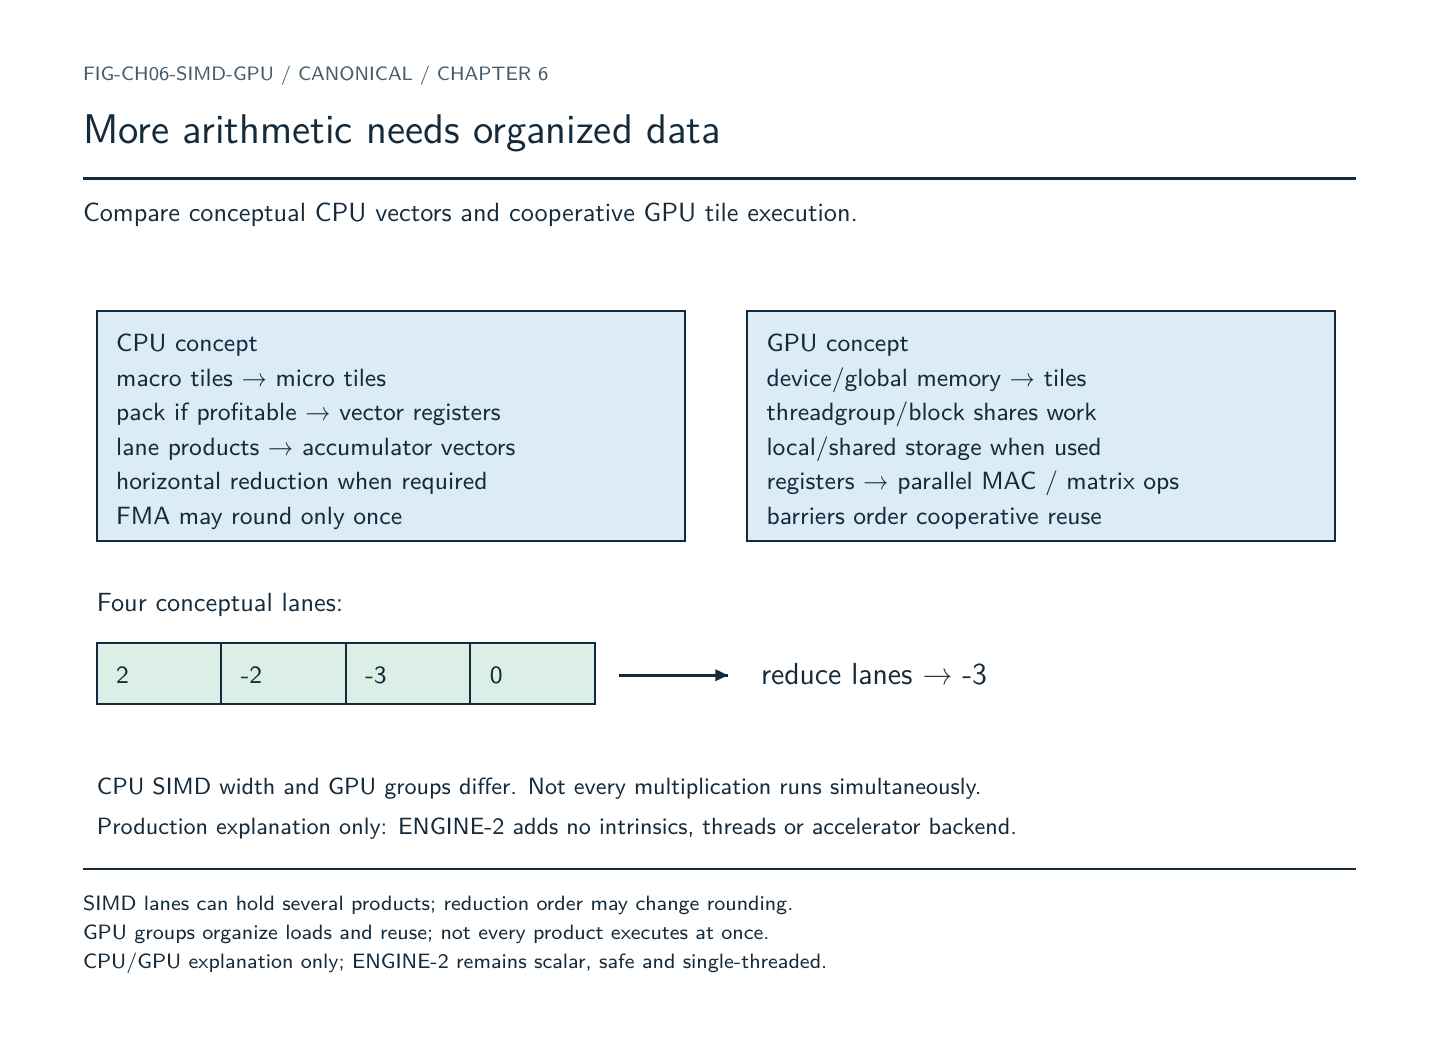
\begin{tikzpicture}[x=.5pt,y=-.5pt]
\path[use as bounding box] (0,0) rectangle (1000,720);
\path[fill=white,draw=none,line width=0.5pt] (0.0,0.0) rectangle (1000.0,720.0);
\node[inner sep=0pt,outer sep=0pt,anchor=base west,text={rgb,255:red,70;green,92;blue,107},font=\sffamily\fontsize{7.0}{8.4}\selectfont] at (40,38) {FIG-CH06-SIMD-GPU  /  CANONICAL / CHAPTER 6};
\node[inner sep=0pt,outer sep=0pt,anchor=base west,text={rgb,255:red,21;green,43;blue,60},font=\sffamily\fontsize{15.0}{18.0}\selectfont] at (40,84) {More arithmetic needs organized data};
\draw[fill=none,draw={rgb,255:red,21;green,43;blue,60},line width=0.75pt] (40,109) -- (960,109);
\node[inner sep=0pt,outer sep=0pt,anchor=base west,text={rgb,255:red,21;green,43;blue,60},font=\sffamily\fontsize{9.5}{11.4}\selectfont] at (40,140) {Compare conceptual CPU vectors and cooperative GPU tile execution.};
\path[fill={rgb,255:red,220;green,236;blue,247},draw={rgb,255:red,21;green,43;blue,60},line width=0.7pt] (50.0,205.0) rectangle (475.0,371.0);
\node[inner sep=0pt,outer sep=0pt,anchor=base west,text={rgb,255:red,21;green,43;blue,60},font=\sffamily\fontsize{9.0}{10.799999999999999}\selectfont] at (64,234) {CPU concept};
\node[inner sep=0pt,outer sep=0pt,anchor=base west,text={rgb,255:red,21;green,43;blue,60},font=\sffamily\fontsize{9.0}{10.799999999999999}\selectfont] at (64,259) {macro tiles → micro tiles};
\node[inner sep=0pt,outer sep=0pt,anchor=base west,text={rgb,255:red,21;green,43;blue,60},font=\sffamily\fontsize{9.0}{10.799999999999999}\selectfont] at (64,284) {pack if profitable → vector registers};
\node[inner sep=0pt,outer sep=0pt,anchor=base west,text={rgb,255:red,21;green,43;blue,60},font=\sffamily\fontsize{9.0}{10.799999999999999}\selectfont] at (64,309) {lane products → accumulator vectors};
\node[inner sep=0pt,outer sep=0pt,anchor=base west,text={rgb,255:red,21;green,43;blue,60},font=\sffamily\fontsize{9.0}{10.799999999999999}\selectfont] at (64,334) {horizontal reduction when required};
\node[inner sep=0pt,outer sep=0pt,anchor=base west,text={rgb,255:red,21;green,43;blue,60},font=\sffamily\fontsize{9.0}{10.799999999999999}\selectfont] at (64,359) {FMA may round only once};
\path[fill={rgb,255:red,220;green,236;blue,247},draw={rgb,255:red,21;green,43;blue,60},line width=0.7pt] (520.0,205.0) rectangle (945.0,371.0);
\node[inner sep=0pt,outer sep=0pt,anchor=base west,text={rgb,255:red,21;green,43;blue,60},font=\sffamily\fontsize{9.0}{10.799999999999999}\selectfont] at (534,234) {GPU concept};
\node[inner sep=0pt,outer sep=0pt,anchor=base west,text={rgb,255:red,21;green,43;blue,60},font=\sffamily\fontsize{9.0}{10.799999999999999}\selectfont] at (534,259) {device/global memory → tiles};
\node[inner sep=0pt,outer sep=0pt,anchor=base west,text={rgb,255:red,21;green,43;blue,60},font=\sffamily\fontsize{9.0}{10.799999999999999}\selectfont] at (534,284) {threadgroup/block shares work};
\node[inner sep=0pt,outer sep=0pt,anchor=base west,text={rgb,255:red,21;green,43;blue,60},font=\sffamily\fontsize{9.0}{10.799999999999999}\selectfont] at (534,309) {local/shared storage when used};
\node[inner sep=0pt,outer sep=0pt,anchor=base west,text={rgb,255:red,21;green,43;blue,60},font=\sffamily\fontsize{9.0}{10.799999999999999}\selectfont] at (534,334) {registers → parallel MAC / matrix ops};
\node[inner sep=0pt,outer sep=0pt,anchor=base west,text={rgb,255:red,21;green,43;blue,60},font=\sffamily\fontsize{9.0}{10.799999999999999}\selectfont] at (534,359) {barriers order cooperative reuse};
\node[inner sep=0pt,outer sep=0pt,anchor=base west,text={rgb,255:red,21;green,43;blue,60},font=\sffamily\fontsize{9.5}{11.4}\selectfont] at (50,422) {Four conceptual lanes:};
\path[fill={rgb,255:red,220;green,239;blue,231},draw={rgb,255:red,21;green,43;blue,60},line width=0.7pt] (50.0,445.0) rectangle (140.0,489.0);
\node[inner sep=0pt,outer sep=0pt,anchor=base west,text={rgb,255:red,21;green,43;blue,60},font=\sffamily\fontsize{9.0}{10.799999999999999}\selectfont] at (64,474) {2};
\path[fill={rgb,255:red,220;green,239;blue,231},draw={rgb,255:red,21;green,43;blue,60},line width=0.7pt] (140.0,445.0) rectangle (230.0,489.0);
\node[inner sep=0pt,outer sep=0pt,anchor=base west,text={rgb,255:red,21;green,43;blue,60},font=\sffamily\fontsize{9.0}{10.799999999999999}\selectfont] at (154,474) {-2};
\path[fill={rgb,255:red,220;green,239;blue,231},draw={rgb,255:red,21;green,43;blue,60},line width=0.7pt] (230.0,445.0) rectangle (320.0,489.0);
\node[inner sep=0pt,outer sep=0pt,anchor=base west,text={rgb,255:red,21;green,43;blue,60},font=\sffamily\fontsize{9.0}{10.799999999999999}\selectfont] at (244,474) {-3};
\path[fill={rgb,255:red,220;green,239;blue,231},draw={rgb,255:red,21;green,43;blue,60},line width=0.7pt] (320.0,445.0) rectangle (410.0,489.0);
\node[inner sep=0pt,outer sep=0pt,anchor=base west,text={rgb,255:red,21;green,43;blue,60},font=\sffamily\fontsize{9.0}{10.799999999999999}\selectfont] at (334,474) {0};
\draw[fill=none,draw={rgb,255:red,21;green,43;blue,60},line width=1.25pt] (427,468) -- (506,468);
\path[fill={rgb,255:red,21;green,43;blue,60},draw=none,line width=0.5pt] (506.00,468.00) -- (497.00,472.35) -- (497.00,463.65) -- cycle;
\node[inner sep=0pt,outer sep=0pt,anchor=base west,text={rgb,255:red,21;green,43;blue,60},font=\sffamily\fontsize{11.0}{13.2}\selectfont] at (530,475) {reduce lanes → -3};
\node[inner sep=0pt,outer sep=0pt,anchor=base west,text={rgb,255:red,21;green,43;blue,60},font=\sffamily\fontsize{8.5}{10.2}\selectfont] at (50,554) {CPU SIMD width and GPU groups differ. Not every multiplication runs simultaneously.};
\node[inner sep=0pt,outer sep=0pt,anchor=base west,text={rgb,255:red,21;green,43;blue,60},font=\sffamily\fontsize{8.5}{10.2}\selectfont] at (50,583) {Production explanation only: ENGINE-2 adds no intrinsics, threads or accelerator backend.};
\draw[fill=none,draw={rgb,255:red,21;green,43;blue,60},line width=0.75pt] (40,608) -- (960,608);
\node[inner sep=0pt,outer sep=0pt,anchor=base west,text={rgb,255:red,21;green,43;blue,60},font=\sffamily\fontsize{7.5}{9.0}\selectfont] at (40,638) {SIMD lanes can hold several products; reduction order may change rounding.};
\node[inner sep=0pt,outer sep=0pt,anchor=base west,text={rgb,255:red,21;green,43;blue,60},font=\sffamily\fontsize{7.5}{9.0}\selectfont] at (40,659) {GPU groups organize loads and reuse; not every product executes at once.};
\node[inner sep=0pt,outer sep=0pt,anchor=base west,text={rgb,255:red,21;green,43;blue,60},font=\sffamily\fontsize{7.5}{9.0}\selectfont] at (40,680) {CPU/GPU explanation only; ENGINE-2 remains scalar, safe and single-threaded.};
\end{tikzpicture}
}\caption{Conceptual CPU vector work and GPU cooperative tile work, explicitly outside ENGINE-2 implementation scope.}\end{figure}

A GPU assigns pieces of an output tile to cooperating groups of threads.
A common tiled design loads operand regions from device/global memory,
stages reusable data in shared or threadgroup storage, and keeps partial
outputs in registers. Thread indexing must make collective memory
accesses efficient; barriers order cooperative reuse where required.
NVIDIA's worked matrix multiplication examples distinguish improved
global access from eliminating redundant loads. These are distinct
benefits, not evidence collected by this chapter.
\href{https://docs.nvidia.com/cuda/cuda-c-best-practices-guide/index.html\#shared-memory-in-matrix-multiplication-c-ab}{CUDA
Best Practices, shared-memory matrix multiplication}

CUTLASS explains a hierarchy of thread-block, warp, and thread tiles,
with register accumulators inside the larger tile. Specialized matrix
multiply-accumulate instructions can consume matrix fragments, including
mixed-precision combinations, rather than one scalar product per source
statement. Storage, multiplication, and accumulation types must then be
specified independently. This is a conceptual preview, not a claim that
all GPU kernels use one staging scheme or numerical type.
\href{https://developer.nvidia.com/blog/cutlass-linear-algebra-cuda/}{NVIDIA's
CUTLASS explanation}

At the pinned GGML revision, CUDA has distinct floating-point/quantized
matrix-vector and matrix-matrix branches and a cuBLAS route. Metal's
\texttt{\seqsplit{ggml\_metal\_op\_mul\_mat}} examines dimensions,
operand types and eligibility; its small-batch branches differ from its
matrix-matrix paths. The literal thresholds in that source belong to
that implementation, not to ENGINE-2's Apple M1 crossover experiment. A
CUDA warp and Metal SIMD group are not a portable synonym for the
chapter's four drawn lanes.

The scheduling problem includes launch cost, data residency, transfers
when needed, occupancy, register pressure, tails, and synchronization.
More nominal arithmetic capacity cannot rescue every tiny or skinny
workload. Conversely, large regular work can amortize costs and exploit
reuse unavailable to one isolated vector. Neither statement supplies a
speedup number. Measure the actual shape, representation, backend,
precision and end-to-end boundary.

\subsection{Why this is still not production
GEMM}\label{why-this-is-still-not-production-gemm}

ENGINE-2 is dependency-free, scalar, single-threaded, CPU-only, and safe
Rust. It does not pack panels, use SIMD intrinsics, specialize register
microkernels, call BLAS, use Apple's Accelerate framework, spawn Rayon
workers, dispatch by CPU feature, fuse bias, or offload to a GPU. It
also allocates a new output on each public call.

Production GEMM commonly layers:

\begin{enumerate}
\def\labelenumi{\arabic{enumi}.}
\tightlist
\item
  semantic validation and transpose/layout interpretation;
\item
  packing into kernel-friendly panels;
\item
  cache blocking;
\item
  register blocking and vector microkernels;
\item
  thread partitioning and NUMA policy;
\item
  architecture and accelerator dispatch;
\item
  fusion with adjacent operations where semantics permit.
\end{enumerate}

The full
\href{https://github.com/hermonai/inside-the-llm-engine/blob/astra-visual-rewrite/diagrams/linear/optimization-ladder.txt}{optimization
ladder diagram} marks exactly where the milestone stops. Previewing
later rungs is useful; implementing them now would violate the chapter's
controlled experiment.

Packing deserves particular caution. A packed layout can make a
microkernel fast but costs time and memory to produce. Immutable model
weights may amortize packing across many calls; one-off activations may
not. That accounting belongs with the future kernel that actually packs.
The same principle applies to thread launch and GPU transfer: overhead
is part of the workload, not an asterisk after the timing.

\subsection{Engineering failures}\label{engineering-failures}

\subsubsection{Inner dimensions do not
agree}\label{inner-dimensions-do-not-agree}

Code receives \texttt{{[}M,K₁{]}\ ×\ {[}K₂,N{]}} and loops to one
operand's bound. It either indexes outside the other view or computes a
truncated fiction. ENGINE-2 returns
\texttt{\seqsplit{InnerDimensionMismatch}} before allocation.

\subsubsection{The right offset uses the wrong
dimension}\label{the-right-offset-uses-the-wrong-dimension}

Writing \texttt{right{[}k\ *\ K\ +\ j{]}} instead of
\texttt{right{[}k\ *\ N\ +\ j{]}} can pass square tests. Asymmetric
\texttt{{[}2,3{]}\ ×\ {[}3,2{]}} and property grids expose it.

\subsubsection{Tile tails disappear}\label{tile-tails-disappear}

Loops assume dimensions divide the tile exactly. Boundary rows or
columns stay zero, or an unchecked implementation crosses storage. The
\texttt{{[}5,7{]}\ ×\ {[}7,3{]}} fixture with \texttt{{[}4,4,2{]}}
blocks creates tails on every axis.

\subsubsection{Faster but wrong}\label{faster-but-wrong}

A benchmark times an optimized path without comparing output. Dead work,
missing tiles, or stale accumulation can look exceptionally fast. The
harness checks outputs first and consumes checksums so the result
remains observable.

\subsubsection{Allocation is counted on one side
only}\label{allocation-is-counted-on-one-side-only}

One candidate reuses a prepared output while another allocates and
zeros. The comparison attributes memory-management policy to loop order.
The Chapter 6 harness includes output allocation for both direct
variants and documents the blocked API's allocation.

\subsubsection{Debug performance is
reported}\label{debug-performance-is-reported}

Rust debug builds prioritize diagnostics and overflow checks rather than
optimized execution. Chapter performance records use
\texttt{cargo\ run\ -\/-release} and identify compiler and flags.

\subsubsection{FLOPs become
instructions}\label{flops-become-instructions}

The conventional \texttt{2MKN} count is described as retired operations,
even though FMA, vector width, compiler transformations, and loop
control make that false. The book calls it an effective work model.

\subsubsection{Tolerance hides a structural
defect}\label{tolerance-hides-a-structural-defect}

A generous threshold makes wrong indexing ``equivalent.'' ENGINE-2
combines a tight bounded tolerance with exact hand fixtures, shape
assertions, typed failures, and full-vector comparison.

\subsubsection{Benchmark order becomes cache
policy}\label{benchmark-order-becomes-cache-policy}

One candidate always runs after another and inherits warmer inputs. The
small harness uses a warm process but does not fully randomize or
control cache state; the records disclose this limitation. Serving
claims would require a stronger protocol and distributions, not just
medians from this microbenchmark.

\subsection{Common misconceptions, checked against this
chapter}\label{common-misconceptions-checked-against-this-chapter}

\begin{itemize}
\tightlist
\item
  \textbf{``GEMV is trivial.''} Its equation is compact; the physical
  GEMV trace still requires correct orientation, checked offsets,
  ownership and a reduction.
\item
  \textbf{``GEMM is just more GEMV.''} Repeated columns prove
  mathematical equivalence; the outer-product view exposes a different
  opportunity to reuse each weight.
\item
  \textbf{``More FLOPs means slower.''} The historical N sweep separates
  total work, latency and attained throughput. None alone predicts the
  other two.
\item
  \textbf{``Asymptotic complexity selects the fastest loop.''} IJK and
  IKJ have the same contribution count, yet their recorded medians
  differ. Constants and address order remain observable below the
  asymptotic notation.
\item
  \textbf{``Blocking always helps.''} The crossover record includes
  losses at sizes 8 and 16, and the tile sweep includes a losing tile 8.
\item
  \textbf{``The default block size is optimal.''} Tile 64, not the
  default 32, won the recorded 192-cube sweep. One sweep cannot
  establish a portable default.
\item
  \textbf{``SIMD changes the equation.''} The same contributions can
  occupy vector lanes; scheduling and F32 grouping change, not the
  intended contraction.
\item
  \textbf{``Matrix multiplication is one instruction.''} The
  source-to-kernel map distinguishes a graph node from loads,
  arithmetic, stores and dispatch.
\item
  \textbf{``A GPU multiplies everything at once.''} The hardware plate
  shows finite tiles, registers and cooperative groups; launch and data
  movement still cost.
\item
  \textbf{``Equivalent kernels must be bit-identical.''} The executable
  reassociation and FMA examples show why numerical equivalence needs a
  stated policy.
\item
  \textbf{``Transpose always copies.''} Chapter 5's metadata view
  remains valid for the reference; blocked layout rejection makes any
  later copy explicit.
\item
  \textbf{``Quantization changes matrix shape.''} GGML's logical extents
  survive a representation change; bytes and approximation error require
  separate rules.
\item
  \textbf{``llama.cpp defines multiplication.''} The equation precedes
  the library. The source comparison translates its axes and dispatch,
  not the mathematics.
\end{itemize}

\subsection{Labs and exercises}\label{labs-and-exercises}

The chapter's executable sequence is:

\begin{itemize}
\tightlist
\item
  \href{https://github.com/hermonai/inside-the-llm-engine/blob/astra-visual-rewrite/labs/lab-22-dot-product.md}{Lab
  22 --- Dot Product}, CHECK;
\item
  \href{https://github.com/hermonai/inside-the-llm-engine/blob/astra-visual-rewrite/labs/lab-23-gemv-by-hand.md}{Lab
  23 --- GEMV by Hand}, CHECK;
\item
  \href{https://github.com/hermonai/inside-the-llm-engine/blob/astra-visual-rewrite/labs/lab-24-gemm-by-hand.md}{Lab
  24 --- GEMM by Hand}, BUILD;
\item
  \href{https://github.com/hermonai/inside-the-llm-engine/blob/astra-visual-rewrite/labs/lab-25-loop-order.md}{Lab
  25 --- Loop Order}, BUILD;
\item
  \href{https://github.com/hermonai/inside-the-llm-engine/blob/astra-visual-rewrite/labs/lab-26-blocked-gemm.md}{Lab
  26 --- Blocked GEMM}, BUILD;
\item
  \href{https://github.com/hermonai/inside-the-llm-engine/blob/astra-visual-rewrite/labs/lab-27-break-the-kernel.md}{Lab
  27 --- Break the Kernel}, BREAK;
\item
  \href{https://github.com/hermonai/inside-the-llm-engine/blob/astra-visual-rewrite/labs/lab-28-kernel-equivalence.md}{Lab
  28 --- Kernel Equivalence}, CHECK;
\item
  \href{https://github.com/hermonai/inside-the-llm-engine/blob/astra-visual-rewrite/labs/lab-29-gemv-vs-gemm.md}{Lab
  29 --- GEMV Versus GEMM}, EXTEND.
\end{itemize}

Further exercises:

\begin{enumerate}
\def\labelenumi{\arabic{enumi}.}
\tightlist
\item
  Enumerate the physical \(B\) offsets for all six loop orders on
  \texttt{{[}2,3{]}\ ×\ {[}3,4{]}}. Classify only the innermost access;
  do not predict a universal winner.
\item
  Derive the exact multiplication and addition counts for \(K=0\),
  \(K=1\), and \(K>1\). Compare them with the conventional \(2MKN\)
  model.
\item
  For a hypothetical 32 KiB cache, solve for cubic \texttt{f32} tile
  sizes whose ideal three-tile payload fits. List at least three reasons
  the calculation does not guarantee residency or speed.
\item
  Add a deterministic cancellation-heavy fixture. Compare ascending and
  descending K reductions and explain the observed error.
\item
  Design an output-buffer API that permits reuse. State the aliasing,
  initialization, shape, and failure rules before writing code.
\item
  Explain when explicitly materializing a transpose once could be
  profitable across many products. Include the copy in a break-even
  model.
\item
  Extend the benchmark with rectangles where \(M\ll N\) and \(N\ll M\).
  Preserve negative results and avoid tuning a global default from one
  host.
\item
  Read the Netlib SGEMM interface and list the features ENGINE-2
  intentionally omits. Explain why omission makes this chapter's
  contract easier to prove.
\end{enumerate}

\subsection{What we still have not
built}\label{what-we-still-have-not-built-1}

At the Chapter 6 curriculum boundary, ENGINE-2 is a linear algebra
kernel layer, not a Transformer. This milestone adds no normalization,
learned Transformer block, attention, Q/K/V projections, causal mask,
RoPE, KV cache, GGUF loader, quantized storage, SIMD, BLAS integration,
threading, GPU provider, autograd, or distributed execution.

It also does not choose kernels dynamically. \texttt{gemv\_reference}
and \texttt{matmul\_blocked} are explicit calls with explicit contracts.
A future provider may use shape, dtype, layout, hardware, and measured
crossover information to select an implementation, but silently
inventing that policy here would make the first optimization cycle
harder to see.

\subsection{Summary}\label{summary-5}

Matrix multiplication is a family of reductions. Dot product reduces two
length-\(K\) vectors to one scalar. GEMV applies one row dot product per
output element. GEMM applies one row/column dot product per output cell:

\[
C_{ij}=\sum_{k=0}^{K-1}A_{ik}B_{kj}.
\]

The conventional work models are \(2MK\) FLOPs for GEMV and \(2MKN\)
FLOPs for GEMM. Those counts do not determine elapsed time. Row-major
offset progression, spatial locality, temporal reuse, working-set size,
and kernel overhead all matter. Arithmetic intensity connects work to
modeled byte movement; the Roofline model previews why low-reuse
operations can be bandwidth constrained.

ENGINE-2 now provides transparent dot, GEMV, and GEMM reference kernels
plus a scalar blocked GEMM. The reference path supports valid strided
views. The blocked path requires canonical storage and never hides
materialization. Both return explicit owned outputs, use checked shape
boundaries, preserve zero-size semantics, and report typed failures.

The optimized path did not replace its oracle. Deterministic property
tests, tail fixtures, the independent Python implementation, numerical
tolerances, and the preserved ENGINE-1 logits form its equivalence gate.
Release measurements then showed both wins and losses: loop order
mattered on the recorded host, blocking hurt tiny matrices, tile choice
mattered, and reuse opportunity did not automatically become throughput.

\begin{quote}
\textbf{FIRST PRINCIPLE} Count the arithmetic, trace the bytes, prove
the substitution, and only then believe the stopwatch.
\end{quote}

\subsection{Chapter 7 preview}\label{chapter-7-preview}

The completed boundary can be read as a compact execution map:

\begin{center}\begin{adjustbox}{max width=\linewidth}% Legacy topology preserved as native vectors and typeset labels.
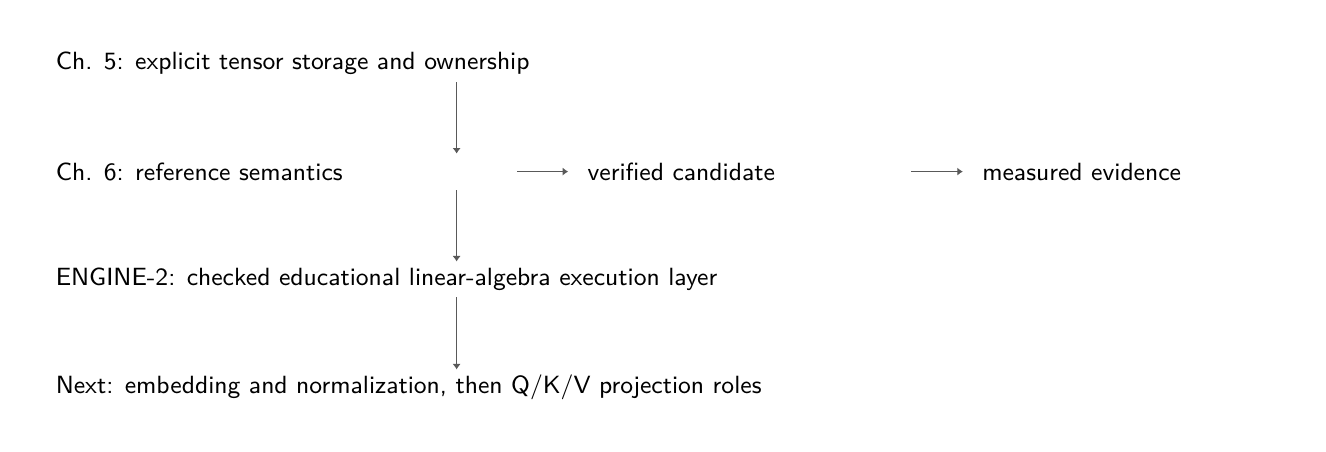
\begin{tikzpicture}[x=6.2pt,y=-13pt,draw=black!65,line width=.45pt]
\path[use as bounding box] (-1,-1) rectangle (73,10);
\node[anchor=west,inner sep=0pt,font=\sffamily\fontsize{9}{11}\selectfont] at (0.6,0) {\begin{adjustbox}{max width=272.8pt}Ch. 5: explicit tensor storage and ownership\end{adjustbox}};
\draw (24,1) -- (24,0.5);
\draw (24,1) -- (24,1.5);
\draw[-{Latex[length=2pt,width=3pt]}] (24,1.5) -- (24,2.5);
\draw (28,3) -- (27.5,3);
\draw (28,3) -- (28.5,3);
\draw (29,3) -- (28.5,3);
\draw (29,3) -- (29.5,3);
\draw[-{Latex[length=2pt,width=3pt]}] (29.5,3) -- (30.5,3);
\draw (51,3) -- (50.5,3);
\draw (51,3) -- (51.5,3);
\draw (52,3) -- (51.5,3);
\draw (52,3) -- (52.5,3);
\draw[-{Latex[length=2pt,width=3pt]}] (52.5,3) -- (53.5,3);
\node[anchor=west,inner sep=0pt,font=\sffamily\fontsize{9}{11}\selectfont] at (0.6,3) {\begin{adjustbox}{max width=161.20000000000002pt}Ch. 6: reference semantics\end{adjustbox}};
\node[anchor=west,inner sep=0pt,font=\sffamily\fontsize{9}{11}\selectfont] at (31.6,3) {\begin{adjustbox}{max width=111.60000000000001pt}verified candidate\end{adjustbox}};
\node[anchor=west,inner sep=0pt,font=\sffamily\fontsize{9}{11}\selectfont] at (54.6,3) {\begin{adjustbox}{max width=105.4pt}measured evidence\end{adjustbox}};
\draw (24,4) -- (24,3.5);
\draw (24,4) -- (24,4.5);
\draw[-{Latex[length=2pt,width=3pt]}] (24,4.5) -- (24,5.5);
\node[anchor=west,inner sep=0pt,font=\sffamily\fontsize{9}{11}\selectfont] at (0.6,6) {\begin{adjustbox}{max width=372.0pt}ENGINE-2: checked educational linear-algebra execution layer\end{adjustbox}};
\draw (24,7) -- (24,6.5);
\draw (24,7) -- (24,7.5);
\draw[-{Latex[length=2pt,width=3pt]}] (24,7.5) -- (24,8.5);
\node[anchor=west,inner sep=0pt,font=\sffamily\fontsize{9}{11}\selectfont] at (0.6,9) {\begin{adjustbox}{max width=384.40000000000003pt}Next: embedding and normalization, then Q/K/V projection roles\end{adjustbox}};
\end{tikzpicture}
\end{adjustbox}\end{center}

ENGINE-2 means transparent reference semantics over explicit tensor
storage, an independently verified blocked candidate, and bounded
measurements of locality-sensitive work. It is more than four function
names and less than a production backend.

We can now store tensors honestly and apply checked linear
transformations. The next missing primitive is normalization. Chapter 7
will build RMSNorm from first principles: squares, mean square, epsilon,
reciprocal square root, learned scale, precision, and its place around
model blocks.

That chapter will reuse ENGINE-2's discipline---reference semantics
before optimization---but it does not begin here. Matrix multiplication
remains the only new numerical operator family in this milestone.

In the book's progression, Chapter 5 establishes where values live;
Chapter 6 shows how computation walks them; Chapter 7 uses parameters
and activations in embedding and normalization; Chapter 8 will give
learned projections Q/K/V roles. The existing Chapter 7 code remains a
regression, not newly regenerated work in this edition.

\subsection{References}\label{references-3}

\begin{itemize}
\tightlist
\item
  Netlib, \href{https://www.netlib.org/blas/}{Basic Linear Algebra
  Subprograms}, including the Level 2 GEMV and Level 3 GEMM families.
\item
  Netlib LAPACK documentation,
  \href{https://netlib.org/lapack/explore-html/d7/dda/group__gemv_ga0d35d880b663ad18204bb23bd186e380.html}{SGEMV
  interface and reference source}.
\item
  Netlib LAPACK documentation,
  \href{https://www.netlib.org/lapack/explore-html/d4/de2/sgemm_8f_source.html}{SGEMM
  reference source}.
\item
  Samuel Williams, Andrew Waterman, and David Patterson,
  \href{https://www2.eecs.berkeley.edu/Pubs/TechRpts/2008/EECS-2008-134.pdf}{Roofline:
  An Insightful Visual Performance Model for Multicore Architectures}.
\item
  Intel,
  \href{https://www.intel.com/content/www/us/en/docs/advisor/cookbook/2023-0/optimize-memory-access-patterns.html}{Optimize
  Memory Access Patterns}, for loop interchange and cache blocking
  examples.
\item
  Oracle,
  \href{https://docs.oracle.com/cd/E37069_01/html/E39019/gnabm.html}{When
  \texttt{(-x)\ *\ (-y)} Is Not \texttt{x\ *\ y}}, for floating-point
  reassociation constraints.
\item
  Project research note,
  \href{https://github.com/hermonai/inside-the-llm-engine/blob/astra-visual-rewrite/research/part-02/chapter-06-matrix-multiplication-the-engine-room.md}{Chapter
  6 --- Matrix Multiplication: The Engine Room}, with commit-pinned
  Hermon and GGML paths.
\item
  Project benchmark records:
  \href{https://github.com/hermonai/inside-the-llm-engine/blob/astra-visual-rewrite/research/benchmarks/chapter-06-loop-order.md}{loop
  order},
  \href{https://github.com/hermonai/inside-the-llm-engine/blob/astra-visual-rewrite/research/benchmarks/chapter-06-blocked-matmul.md}{blocked
  multiplication}, and
  \href{https://github.com/hermonai/inside-the-llm-engine/blob/astra-visual-rewrite/research/benchmarks/chapter-06-gemv-vs-gemm.md}{GEMV
  versus GEMM}.
\end{itemize}

\clearpage

\section{Chapter 7 --- Embeddings and
Normalization}\label{chapter-7-embeddings-and-normalization}

Chapter 2 ended with integers. A tokenizer transformed UTF-8 bytes into
token identities under a model-specific vocabulary contract. Chapter 3
used one of those identities to select a hidden vector, but its purpose
was to make an entire language-model forward pass small enough to
calculate by hand. Now we can inspect that first numerical step as an
engine operation in its own right.

A token ID is not a small activation. Multiplying the integer
\texttt{128} by a model weight does not recover what token 128
``means.'' The integer is an addressable symbol. The model's
\textbf{embedding table} stores one learned floating-point row for each
symbol. A checked lookup crosses from discrete token space into the
continuous model space in which the network computes.

Once there, scale matters. A vector and a hundred-times-larger copy
point in the same direction, but their components drive later arithmetic
at very different magnitudes. Transformer architectures commonly place
normalization around learned transformations to control that scale. This
chapter builds \textbf{RMSNorm} from squares, a mean, a square root, a
reciprocal, and a learned element-wise scale. There is no hidden
framework call.

These operators are short. Their contracts are not. We need to know
which axes mean vocabulary and model width, which bytes a row uses,
whether the result aliases weights, what happens to an empty dimension,
where epsilon appears, which precision performs the reduction, and what
finite values can still overflow. Those decisions become assumptions of
every later Transformer chapter.

\begin{quote}
\textbf{FIRST PRINCIPLE} Tokenization chooses a discrete model symbol.
Embedding lookup materializes that symbol's learned model-space vector.
Normalization then changes the vector's scale under an explicit
numerical contract; it does not invent its meaning or clip its
coordinates.
\end{quote}

\subsection{The first learned vector}\label{the-first-learned-vector}

\begin{figure}[H]\centering\resizebox{\linewidth}{!}{% Generated from figures/generated/ch07-journey.svg; do not hand edit.
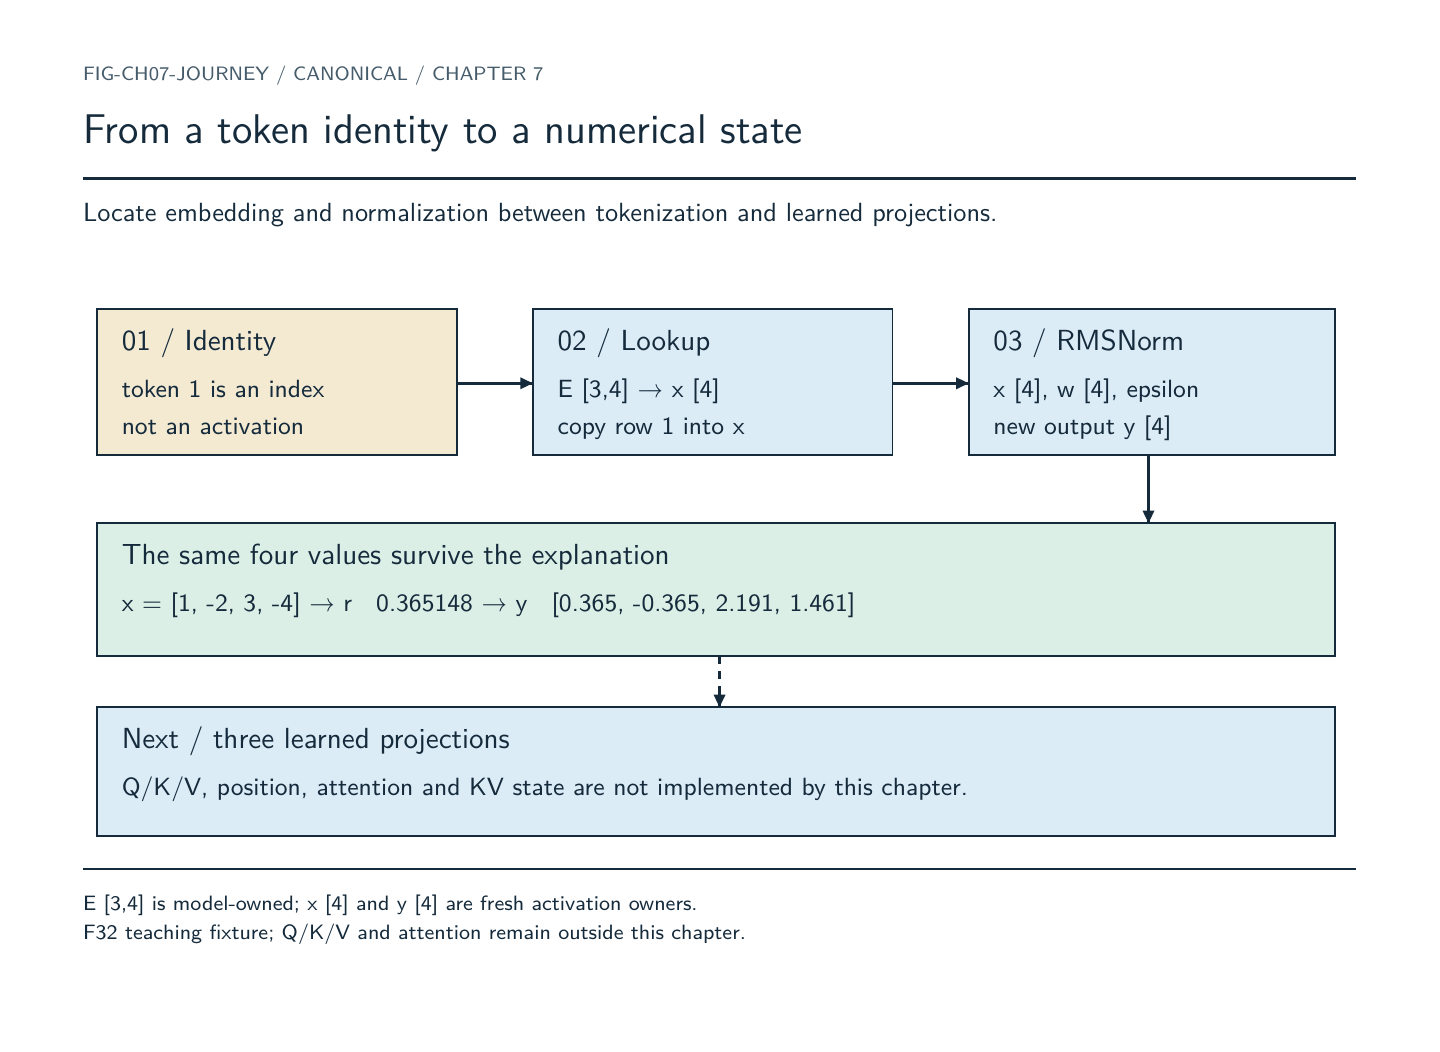
\begin{tikzpicture}[x=.5pt,y=-.5pt]
\path[use as bounding box] (0,0) rectangle (1000,720);
\path[fill=white,draw=none,line width=0.5pt] (0.0,0.0) rectangle (1000.0,720.0);
\node[inner sep=0pt,outer sep=0pt,anchor=base west,text={rgb,255:red,70;green,92;blue,107},font=\sffamily\fontsize{7.0}{8.4}\selectfont] at (40,38) {FIG-CH07-JOURNEY  /  CANONICAL / CHAPTER 7};
\node[inner sep=0pt,outer sep=0pt,anchor=base west,text={rgb,255:red,21;green,43;blue,60},font=\sffamily\fontsize{15.0}{18.0}\selectfont] at (40,84) {From a token identity to a numerical state};
\draw[fill=none,draw={rgb,255:red,21;green,43;blue,60},line width=0.75pt] (40,109) -- (960,109);
\node[inner sep=0pt,outer sep=0pt,anchor=base west,text={rgb,255:red,21;green,43;blue,60},font=\sffamily\fontsize{9.5}{11.4}\selectfont] at (40,140) {Locate embedding and normalization between tokenization and learned projections.};
\path[fill={rgb,255:red,244;green,234;blue,210},draw={rgb,255:red,21;green,43;blue,60},line width=0.7pt] (50.0,203.0) rectangle (310.0,309.0);
\node[inner sep=0pt,outer sep=0pt,anchor=base west,text={rgb,255:red,21;green,43;blue,60},font=\sffamily\fontsize{9.5}{11.4}\selectfont] at (64,232) {};
\node[inner sep=0pt,outer sep=0pt,anchor=base west,text={rgb,255:red,21;green,43;blue,60},font=\sffamily\fontsize{10.5}{12.6}\selectfont] at (68,233) {01 / Identity};
\node[inner sep=0pt,outer sep=0pt,anchor=base west,text={rgb,255:red,21;green,43;blue,60},font=\sffamily\fontsize{9.0}{10.799999999999999}\selectfont] at (68,267) {token 1 is an index};
\node[inner sep=0pt,outer sep=0pt,anchor=base west,text={rgb,255:red,21;green,43;blue,60},font=\sffamily\fontsize{9.0}{10.799999999999999}\selectfont] at (68,294) {not an activation};
\path[fill={rgb,255:red,220;green,236;blue,247},draw={rgb,255:red,21;green,43;blue,60},line width=0.7pt] (365.0,203.0) rectangle (625.0,309.0);
\node[inner sep=0pt,outer sep=0pt,anchor=base west,text={rgb,255:red,21;green,43;blue,60},font=\sffamily\fontsize{9.5}{11.4}\selectfont] at (379,232) {};
\node[inner sep=0pt,outer sep=0pt,anchor=base west,text={rgb,255:red,21;green,43;blue,60},font=\sffamily\fontsize{10.5}{12.6}\selectfont] at (383,233) {02 / Lookup};
\node[inner sep=0pt,outer sep=0pt,anchor=base west,text={rgb,255:red,21;green,43;blue,60},font=\sffamily\fontsize{9.0}{10.799999999999999}\selectfont] at (383,267) {E [3,4] → x [4]};
\node[inner sep=0pt,outer sep=0pt,anchor=base west,text={rgb,255:red,21;green,43;blue,60},font=\sffamily\fontsize{9.0}{10.799999999999999}\selectfont] at (383,294) {copy row 1 into x};
\path[fill={rgb,255:red,220;green,236;blue,247},draw={rgb,255:red,21;green,43;blue,60},line width=0.7pt] (680.0,203.0) rectangle (945.0,309.0);
\node[inner sep=0pt,outer sep=0pt,anchor=base west,text={rgb,255:red,21;green,43;blue,60},font=\sffamily\fontsize{9.5}{11.4}\selectfont] at (694,232) {};
\node[inner sep=0pt,outer sep=0pt,anchor=base west,text={rgb,255:red,21;green,43;blue,60},font=\sffamily\fontsize{10.5}{12.6}\selectfont] at (698,233) {03 / RMSNorm};
\node[inner sep=0pt,outer sep=0pt,anchor=base west,text={rgb,255:red,21;green,43;blue,60},font=\sffamily\fontsize{9.0}{10.799999999999999}\selectfont] at (698,267) {x [4], w [4], epsilon};
\node[inner sep=0pt,outer sep=0pt,anchor=base west,text={rgb,255:red,21;green,43;blue,60},font=\sffamily\fontsize{9.0}{10.799999999999999}\selectfont] at (698,294) {new output y [4]};
\draw[fill=none,draw={rgb,255:red,21;green,43;blue,60},line width=1.25pt] (310,257) -- (365,257);
\path[fill={rgb,255:red,21;green,43;blue,60},draw=none,line width=0.5pt] (365.00,257.00) -- (356.00,261.35) -- (356.00,252.65) -- cycle;
\draw[fill=none,draw={rgb,255:red,21;green,43;blue,60},line width=1.25pt] (625,257) -- (680,257);
\path[fill={rgb,255:red,21;green,43;blue,60},draw=none,line width=0.5pt] (680.00,257.00) -- (671.00,261.35) -- (671.00,252.65) -- cycle;
\path[fill={rgb,255:red,220;green,239;blue,231},draw={rgb,255:red,21;green,43;blue,60},line width=0.7pt] (50.0,358.0) rectangle (945.0,454.0);
\node[inner sep=0pt,outer sep=0pt,anchor=base west,text={rgb,255:red,21;green,43;blue,60},font=\sffamily\fontsize{9.5}{11.4}\selectfont] at (64,387) {};
\node[inner sep=0pt,outer sep=0pt,anchor=base west,text={rgb,255:red,21;green,43;blue,60},font=\sffamily\fontsize{10.5}{12.6}\selectfont] at (68,388) {The same four values survive the explanation};
\node[inner sep=0pt,outer sep=0pt,anchor=base west,text={rgb,255:red,21;green,43;blue,60},font=\sffamily\fontsize{9.0}{10.799999999999999}\selectfont] at (68,422) {x = [1, -2, 3, -4]   →   r ≈ 0.365148   →   y ≈ [0.365, -0.365, 2.191, 1.461]};
\path[fill={rgb,255:red,220;green,236;blue,247},draw={rgb,255:red,21;green,43;blue,60},line width=0.7pt] (50.0,491.0) rectangle (945.0,584.0);
\node[inner sep=0pt,outer sep=0pt,anchor=base west,text={rgb,255:red,21;green,43;blue,60},font=\sffamily\fontsize{9.5}{11.4}\selectfont] at (64,520) {};
\node[inner sep=0pt,outer sep=0pt,anchor=base west,text={rgb,255:red,21;green,43;blue,60},font=\sffamily\fontsize{10.5}{12.6}\selectfont] at (68,521) {Next / three learned projections};
\node[inner sep=0pt,outer sep=0pt,anchor=base west,text={rgb,255:red,21;green,43;blue,60},font=\sffamily\fontsize{9.0}{10.799999999999999}\selectfont] at (68,555) {Q/K/V, position, attention and KV state are not implemented by this chapter.};
\draw[fill=none,draw={rgb,255:red,21;green,43;blue,60},line width=1.25pt] (810,309) -- (810,358);
\path[fill={rgb,255:red,21;green,43;blue,60},draw=none,line width=0.5pt] (810.00,358.00) -- (805.65,349.00) -- (814.35,349.00) -- cycle;
\draw[fill=none,draw={rgb,255:red,21;green,43;blue,60},line width=1.25pt,dash pattern=on 3.0pt off 2.5pt] (500,454) -- (500,491);
\path[fill={rgb,255:red,21;green,43;blue,60},draw=none,line width=0.5pt] (500.00,491.00) -- (495.65,482.00) -- (504.35,482.00) -- cycle;
\draw[fill=none,draw={rgb,255:red,21;green,43;blue,60},line width=0.75pt] (40,608) -- (960,608);
\node[inner sep=0pt,outer sep=0pt,anchor=base west,text={rgb,255:red,21;green,43;blue,60},font=\sffamily\fontsize{7.5}{9.0}\selectfont] at (40,638) {E [3,4] is model-owned; x [4] and y [4] are fresh activation owners.};
\node[inner sep=0pt,outer sep=0pt,anchor=base west,text={rgb,255:red,21;green,43;blue,60},font=\sffamily\fontsize{7.5}{9.0}\selectfont] at (40,659) {F32 teaching fixture; Q/K/V and attention remain outside this chapter.};
\end{tikzpicture}
}\caption{Token identity, copied embedding and normalized activation occupy different boundaries.}\end{figure}

The visual edition follows one deliberately small table through the
whole chapter. It has three vocabulary rows and four coordinates per
row; token 1 selects the existing RMSNorm hand vector
\texttt{{[}1,-2,3,-4{]}}. This is a new connecting fixture, not a
replacement for Chapter 3's three-dimensional tiny model or the original
Chapter 7 table tests. Keeping these identities explicit prevents a
polished diagram from silently changing the engine being explained.

Read the plate as three contracts. An integer identifies a row. Lookup
copies that row into activation storage. RMSNorm creates another
activation under a specified equation. The dashed next-step arrow is a
curriculum boundary, not an implemented Q/K/V call. This is the
model-semantic view; the ownership and physical-address views below
explain what its short arrows cost.

The complete boundary is visible in the
\href{https://github.com/hermonai/inside-the-llm-engine/blob/astra-visual-rewrite/diagrams/transformer/token-to-model-space.txt}{token-to-model-space
diagram}:

\begin{center}\begin{adjustbox}{max width=\linewidth}% Legacy topology preserved as native vectors and typeset labels.
\begin{tikzpicture}[x=6.2pt,y=-13pt,draw=black!65,line width=.45pt]
\path[use as bounding box] (-1,-1) rectangle (79,6);
\draw (0,0) -- (0.5,0);
\draw (0,0) -- (0,0.5);
\draw (1,0) -- (0.5,0);
\draw (1,0) -- (1.5,0);
\draw (2,0) -- (1.5,0);
\draw (2,0) -- (2.5,0);
\draw (3,0) -- (2.5,0);
\draw (3,0) -- (3.5,0);
\draw (4,0) -- (3.5,0);
\draw (4,0) -- (4.5,0);
\draw (5,0) -- (4.5,0);
\draw (5,0) -- (5.5,0);
\draw (6,0) -- (5.5,0);
\draw (6,0) -- (6.5,0);
\draw (7,0) -- (6.5,0);
\draw (7,0) -- (7.5,0);
\draw (8,0) -- (7.5,0);
\draw (8,0) -- (8.5,0);
\draw (9,0) -- (8.5,0);
\draw (9,0) -- (9.5,0);
\draw (10,0) -- (9.5,0);
\draw (10,0) -- (10.5,0);
\draw (11,0) -- (10.5,0);
\draw (11,0) -- (11.5,0);
\draw (12,0) -- (11.5,0);
\draw (12,0) -- (12.5,0);
\draw (13,0) -- (12.5,0);
\draw (13,0) -- (13.5,0);
\draw (14,0) -- (13.5,0);
\draw (14,0) -- (14.5,0);
\draw (15,0) -- (14.5,0);
\draw (15,0) -- (15,0.5);
\draw (31,0) -- (31.5,0);
\draw (31,0) -- (31,0.5);
\draw (32,0) -- (31.5,0);
\draw (32,0) -- (32.5,0);
\draw (33,0) -- (32.5,0);
\draw (33,0) -- (33.5,0);
\draw (34,0) -- (33.5,0);
\draw (34,0) -- (34.5,0);
\draw (35,0) -- (34.5,0);
\draw (35,0) -- (35.5,0);
\draw (36,0) -- (35.5,0);
\draw (36,0) -- (36.5,0);
\draw (37,0) -- (36.5,0);
\draw (37,0) -- (37.5,0);
\draw (38,0) -- (37.5,0);
\draw (38,0) -- (38.5,0);
\draw (39,0) -- (38.5,0);
\draw (39,0) -- (39.5,0);
\draw (40,0) -- (39.5,0);
\draw (40,0) -- (40.5,0);
\draw (41,0) -- (40.5,0);
\draw (41,0) -- (41.5,0);
\draw (42,0) -- (41.5,0);
\draw (42,0) -- (42.5,0);
\draw (43,0) -- (42.5,0);
\draw (43,0) -- (43.5,0);
\draw (44,0) -- (43.5,0);
\draw (44,0) -- (44.5,0);
\draw (45,0) -- (44.5,0);
\draw (45,0) -- (45.5,0);
\draw (46,0) -- (45.5,0);
\draw (46,0) -- (46,0.5);
\node[anchor=west,inner sep=0pt,font=\sffamily\fontsize{9}{11}\selectfont] at (19.6,0) {\begin{adjustbox}{max width=37.2pt}encode\end{adjustbox}};
\node[anchor=west,inner sep=0pt,font=\sffamily\fontsize{9}{11}\selectfont] at (50.6,0) {\begin{adjustbox}{max width=62.0pt}row lookup\end{adjustbox}};
\node[anchor=west,inner sep=0pt,font=\sffamily\fontsize{9}{11}\selectfont] at (64.6,0) {\begin{adjustbox}{max width=55.800000000000004pt}(E [V,D])\end{adjustbox}};
\draw (0,1) -- (0,0.5);
\draw (0,1) -- (0,1.5);
\draw (15,1) -- (15,0.5);
\draw (15,1) -- (15,1.5);
\draw (17,1) -- (16.5,1);
\draw (17,1) -- (17.5,1);
\draw (18,1) -- (17.5,1);
\draw (18,1) -- (18.5,1);
\draw (19,1) -- (18.5,1);
\draw (19,1) -- (19.5,1);
\draw (20,1) -- (19.5,1);
\draw (20,1) -- (20.5,1);
\draw (21,1) -- (20.5,1);
\draw (21,1) -- (21.5,1);
\draw (22,1) -- (21.5,1);
\draw (22,1) -- (22.5,1);
\draw (23,1) -- (22.5,1);
\draw (23,1) -- (23.5,1);
\draw (24,1) -- (23.5,1);
\draw (24,1) -- (24.5,1);
\draw (25,1) -- (24.5,1);
\draw (25,1) -- (25.5,1);
\draw (26,1) -- (25.5,1);
\draw (26,1) -- (26.5,1);
\draw (27,1) -- (26.5,1);
\draw (27,1) -- (27.5,1);
\draw (28,1) -- (27.5,1);
\draw (28,1) -- (28.5,1);
\draw[-{Latex[length=2pt,width=3pt]}] (28.5,1) -- (29.5,1);
\draw (31,1) -- (31,0.5);
\draw (31,1) -- (31,1.5);
\draw (46,1) -- (46,0.5);
\draw (46,1) -- (46,1.5);
\draw (48,1) -- (47.5,1);
\draw (48,1) -- (48.5,1);
\draw (49,1) -- (48.5,1);
\draw (49,1) -- (49.5,1);
\draw (50,1) -- (49.5,1);
\draw (50,1) -- (50.5,1);
\draw (51,1) -- (50.5,1);
\draw (51,1) -- (51.5,1);
\draw (52,1) -- (51.5,1);
\draw (52,1) -- (52.5,1);
\draw (53,1) -- (52.5,1);
\draw (53,1) -- (53.5,1);
\draw (54,1) -- (53.5,1);
\draw (54,1) -- (54.5,1);
\draw (55,1) -- (54.5,1);
\draw (55,1) -- (55.5,1);
\draw (56,1) -- (55.5,1);
\draw (56,1) -- (56.5,1);
\draw (57,1) -- (56.5,1);
\draw (57,1) -- (57.5,1);
\draw (58,1) -- (57.5,1);
\draw (58,1) -- (58.5,1);
\draw (59,1) -- (58.5,1);
\draw (59,1) -- (59.5,1);
\draw (60,1) -- (59.5,1);
\draw (60,1) -- (60.5,1);
\draw (61,1) -- (60.5,1);
\draw (61,1) -- (61.5,1);
\draw[-{Latex[length=2pt,width=3pt]}] (61.5,1) -- (62.5,1);
\node[anchor=west,inner sep=0pt,font=\sffamily\fontsize{9}{11}\selectfont] at (1.6,1) {\begin{adjustbox}{max width=62.0pt}UTF-8 text\end{adjustbox}};
\node[anchor=west,inner sep=0pt,font=\sffamily\fontsize{9}{11}\selectfont] at (32.6,1) {\begin{adjustbox}{max width=55.800000000000004pt}TokenId t\end{adjustbox}};
\node[anchor=west,inner sep=0pt,font=\sffamily\fontsize{9}{11}\selectfont] at (63.6,1) {\begin{adjustbox}{max width=31.0pt}row t\end{adjustbox}};
\draw (0,2) -- (0.5,2);
\draw (0,2) -- (0,1.5);
\draw (1,2) -- (0.5,2);
\draw (1,2) -- (1.5,2);
\draw (2,2) -- (1.5,2);
\draw (2,2) -- (2.5,2);
\draw (3,2) -- (2.5,2);
\draw (3,2) -- (3.5,2);
\draw (4,2) -- (3.5,2);
\draw (4,2) -- (4.5,2);
\draw (5,2) -- (4.5,2);
\draw (5,2) -- (5.5,2);
\draw (6,2) -- (5.5,2);
\draw (6,2) -- (6.5,2);
\draw (7,2) -- (6.5,2);
\draw (7,2) -- (7.5,2);
\draw (8,2) -- (7.5,2);
\draw (8,2) -- (8.5,2);
\draw (9,2) -- (8.5,2);
\draw (9,2) -- (9.5,2);
\draw (10,2) -- (9.5,2);
\draw (10,2) -- (10.5,2);
\draw (11,2) -- (10.5,2);
\draw (11,2) -- (11.5,2);
\draw (12,2) -- (11.5,2);
\draw (12,2) -- (12.5,2);
\draw (13,2) -- (12.5,2);
\draw (13,2) -- (13.5,2);
\draw (14,2) -- (13.5,2);
\draw (14,2) -- (14.5,2);
\draw (15,2) -- (14.5,2);
\draw (15,2) -- (15,1.5);
\draw (31,2) -- (31.5,2);
\draw (31,2) -- (31,1.5);
\draw (32,2) -- (31.5,2);
\draw (32,2) -- (32.5,2);
\draw (33,2) -- (32.5,2);
\draw (33,2) -- (33.5,2);
\draw (34,2) -- (33.5,2);
\draw (34,2) -- (34.5,2);
\draw (35,2) -- (34.5,2);
\draw (35,2) -- (35.5,2);
\draw (36,2) -- (35.5,2);
\draw (36,2) -- (36.5,2);
\draw (37,2) -- (36.5,2);
\draw (37,2) -- (37.5,2);
\draw (38,2) -- (37.5,2);
\draw (38,2) -- (38.5,2);
\draw (39,2) -- (38.5,2);
\draw (39,2) -- (39.5,2);
\draw (40,2) -- (39.5,2);
\draw (40,2) -- (40.5,2);
\draw (41,2) -- (40.5,2);
\draw (41,2) -- (41.5,2);
\draw (42,2) -- (41.5,2);
\draw (42,2) -- (42.5,2);
\draw (43,2) -- (42.5,2);
\draw (43,2) -- (43.5,2);
\draw (44,2) -- (43.5,2);
\draw (44,2) -- (44.5,2);
\draw (45,2) -- (44.5,2);
\draw (45,2) -- (45.5,2);
\draw (46,2) -- (45.5,2);
\draw (46,2) -- (46,1.5);
\draw (70,2) -- (70,1.5);
\draw (70,2) -- (70,2.5);
\node[anchor=west,inner sep=0pt,font=\sffamily\fontsize{9}{11}\selectfont] at (66.6,3) {\begin{adjustbox}{max width=24.8pt}copy\end{adjustbox}};
\draw[-{Latex[length=2pt,width=3pt]}] (69,3.5) -- (69,4.5);
\node[anchor=west,inner sep=0pt,font=\sffamily\fontsize{9}{11}\selectfont] at (59.6,5) {\begin{adjustbox}{max width=111.60000000000001pt}[activation x [D]]\end{adjustbox}};
\end{tikzpicture}
\end{adjustbox}\end{center}

The tokenizer owns text segmentation and the mapping from pieces to
integer IDs. The numerical model owns the embedding table. An ID has
meaning only relative to that pair of artifacts: the same integer can
select an unrelated row in a different model.

Let \(V_{\mathrm{vocab}}\) be the vocabulary size and \(D\) be the model
or embedding dimension. The table is a learned parameter matrix

\[
\mathbf{E}\in\mathbb{R}^{V_{\mathrm{vocab}}\times D}.
\]

For a valid token ID \(t\), lookup produces

\[
\mathbf{x}=\mathbf{E}_{t,:}\in\mathbb{R}^{D},
\qquad 0\le t<V_{\mathrm{vocab}}.
\]

The colon means every column in row \(t\). Written element by element,

\[
x_j=E_{t,j},
\qquad 0\le j<D.
\]

This equation specifies selection, not arithmetic over every table row.
A one-hot vector times \(\mathbf{E}\) is a mathematically equivalent
description, but constructing that mostly-zero vector and performing a
dense product would be a perverse implementation. The engine already has
the row index.

The output is the first \textbf{residual activation}. In a decoder, the
\textbf{residual stream} is the persistent model-width state carried
from one Transformer sublayer to the next. Chapter 7 establishes its
width and normalization; it does not yet build any of the
transformations that consume it.

\subsection{What is physically stored?}\label{what-is-physically-stored}

The table contains floating-point parameters learned during training. It
does not contain source strings, dictionary definitions, or
human-readable facts. Rows can acquire useful geometric relationships,
but an inference engine needs no story about their semantics to execute
lookup. It needs a tensor with valid metadata and a token in range.

The
\href{https://github.com/hermonai/inside-the-llm-engine/blob/astra-visual-rewrite/diagrams/transformer/embedding-logical-layout.txt}{logical
layout} separates the two axes:

\begin{itemize}
\tightlist
\item
  axis 0 has length \(V_{\mathrm{vocab}}\) and is selected by token
  identity;
\item
  axis 1 has length \(D\) and becomes the model-space vector.
\end{itemize}

That is why the semantic shape is \texttt{{[}V,D{]}}, rather than
\texttt{{[}D,V{]}}. The convention matches the operator: selecting
\texttt{table{[}t,:{]}} returns \texttt{D} values. Another system can
store axes differently, but then its metadata and kernel must make that
orientation explicit.

In Tensor Substrate v1, an \texttt{OwnedTensor} uses canonical row-major
storage. An embedding owner therefore reports

\begin{verbatim}
shape   = [V,D]
strides = [D,1]        // measured in elements
dtype   = f32
\end{verbatim}

For base offset zero, the canonical physical element offset is

\[
o(t,j)=tD+j.
\]

Because one \texttt{f32} occupies four bytes, the corresponding byte
displacement from the allocation's first element is

\[
b(t,j)=4(tD+j)\quad[\mathrm{bytes}].
\]

Those equations describe the canonical case. The reference operator
accepts a general validated \texttt{TensorView}, so its actual logical
mapping remains Chapter 5's stride equation:

\[
o(t,j)=b_0+t s_0+j s_1,
\]

where \(b_0\) is the view's base element offset and \(s_0,s_1\) are
nonnegative element strides. The
\href{https://github.com/hermonai/inside-the-llm-engine/blob/astra-visual-rewrite/diagrams/transformer/embedding-physical-layout.txt}{physical-layout
diagram} puts the canonical shortcut beside the general rule. Code calls
checked \texttt{get2(t,j)} instead of reconstructing either formula in
the operator. That keeps extent validation and logical addressing in the
tensor substrate.

For a canonical table, one selected row is physically contiguous:
reading columns \texttt{0..D} walks adjacent \texttt{f32} values. A
strided table can place padding or another logical arrangement between
columns. A zero-stride view can repeat one storage value across an axis.
Tensor Substrate v1 admits those immutable views, so the broad reference
operator defines their behavior instead of quietly assuming stride one.

\subsection{The checked lookup
contract}\label{the-checked-lookup-contract}

\begin{figure}[H]\centering\resizebox{\linewidth}{!}{% Generated from figures/generated/ch07-lookup.svg; do not hand edit.
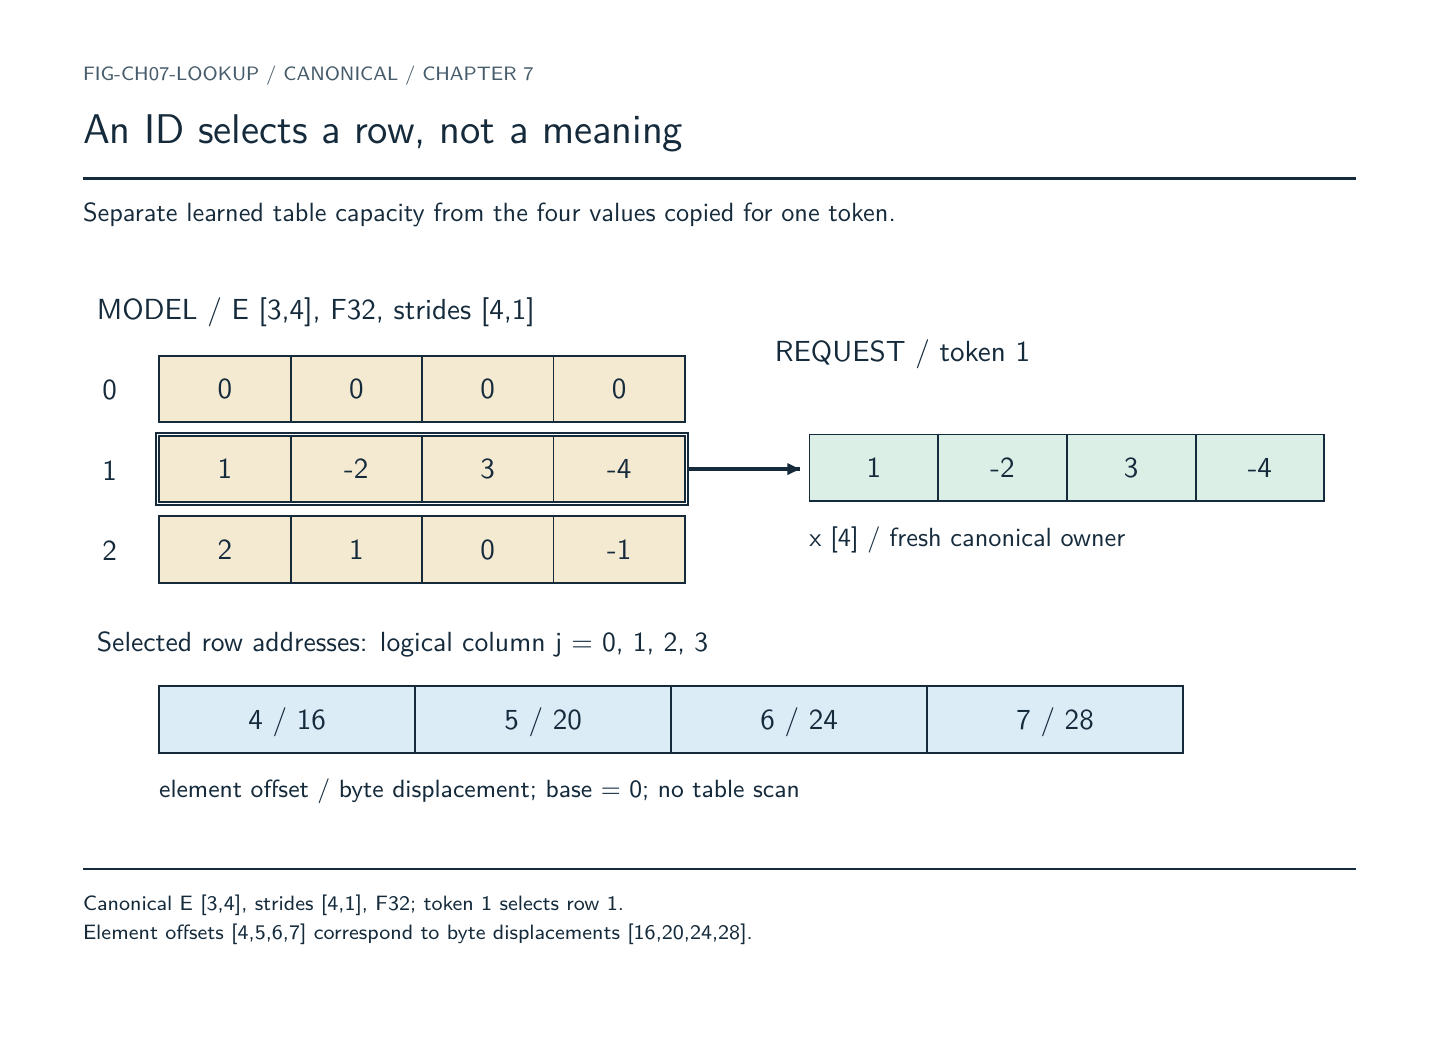
\begin{tikzpicture}[x=.5pt,y=-.5pt]
\path[use as bounding box] (0,0) rectangle (1000,720);
\path[fill=white,draw=none,line width=0.5pt] (0.0,0.0) rectangle (1000.0,720.0);
\node[inner sep=0pt,outer sep=0pt,anchor=base west,text={rgb,255:red,70;green,92;blue,107},font=\sffamily\fontsize{7.0}{8.4}\selectfont] at (40,38) {FIG-CH07-LOOKUP  /  CANONICAL / CHAPTER 7};
\node[inner sep=0pt,outer sep=0pt,anchor=base west,text={rgb,255:red,21;green,43;blue,60},font=\sffamily\fontsize{15.0}{18.0}\selectfont] at (40,84) {An ID selects a row, not a meaning};
\draw[fill=none,draw={rgb,255:red,21;green,43;blue,60},line width=0.75pt] (40,109) -- (960,109);
\node[inner sep=0pt,outer sep=0pt,anchor=base west,text={rgb,255:red,21;green,43;blue,60},font=\sffamily\fontsize{9.5}{11.4}\selectfont] at (40,140) {Separate learned table capacity from the four values copied for one token.};
\node[inner sep=0pt,outer sep=0pt,anchor=base west,text={rgb,255:red,21;green,43;blue,60},font=\sffamily\fontsize{10.5}{12.6}\selectfont] at (50,211) {MODEL / E [3,4], F32, strides [4,1]};
\path[fill={rgb,255:red,244;green,234;blue,210},draw={rgb,255:red,21;green,43;blue,60},line width=0.7pt] (95.0,237.0) rectangle (190.0,285.0);
\node[inner sep=0pt,outer sep=0pt,anchor=base west,text={rgb,255:red,21;green,43;blue,60},font=\sffamily\fontsize{9.5}{11.4}\selectfont] at (109,266) {};
\node[inner sep=0pt,outer sep=0pt,anchor=base,text={rgb,255:red,21;green,43;blue,60},font=\sffamily\fontsize{10.5}{12.6}\selectfont] at (142.5,268) {0};
\path[fill={rgb,255:red,244;green,234;blue,210},draw={rgb,255:red,21;green,43;blue,60},line width=0.7pt] (190.0,237.0) rectangle (285.0,285.0);
\node[inner sep=0pt,outer sep=0pt,anchor=base west,text={rgb,255:red,21;green,43;blue,60},font=\sffamily\fontsize{9.5}{11.4}\selectfont] at (204,266) {};
\node[inner sep=0pt,outer sep=0pt,anchor=base,text={rgb,255:red,21;green,43;blue,60},font=\sffamily\fontsize{10.5}{12.6}\selectfont] at (237.5,268) {0};
\path[fill={rgb,255:red,244;green,234;blue,210},draw={rgb,255:red,21;green,43;blue,60},line width=0.7pt] (285.0,237.0) rectangle (380.0,285.0);
\node[inner sep=0pt,outer sep=0pt,anchor=base west,text={rgb,255:red,21;green,43;blue,60},font=\sffamily\fontsize{9.5}{11.4}\selectfont] at (299,266) {};
\node[inner sep=0pt,outer sep=0pt,anchor=base,text={rgb,255:red,21;green,43;blue,60},font=\sffamily\fontsize{10.5}{12.6}\selectfont] at (332.5,268) {0};
\path[fill={rgb,255:red,244;green,234;blue,210},draw={rgb,255:red,21;green,43;blue,60},line width=0.7pt] (380.0,237.0) rectangle (475.0,285.0);
\node[inner sep=0pt,outer sep=0pt,anchor=base west,text={rgb,255:red,21;green,43;blue,60},font=\sffamily\fontsize{9.5}{11.4}\selectfont] at (394,266) {};
\node[inner sep=0pt,outer sep=0pt,anchor=base,text={rgb,255:red,21;green,43;blue,60},font=\sffamily\fontsize{10.5}{12.6}\selectfont] at (427.5,268) {0};
\node[inner sep=0pt,outer sep=0pt,anchor=base west,text={rgb,255:red,21;green,43;blue,60},font=\sffamily\fontsize{10.5}{12.6}\selectfont] at (54,269) {0};
\path[fill={rgb,255:red,244;green,234;blue,210},draw={rgb,255:red,21;green,43;blue,60},line width=0.7pt] (95.0,295.0) rectangle (190.0,343.0);
\node[inner sep=0pt,outer sep=0pt,anchor=base west,text={rgb,255:red,21;green,43;blue,60},font=\sffamily\fontsize{9.5}{11.4}\selectfont] at (109,324) {};
\node[inner sep=0pt,outer sep=0pt,anchor=base,text={rgb,255:red,21;green,43;blue,60},font=\sffamily\fontsize{10.5}{12.6}\selectfont] at (142.5,326) {1};
\path[fill={rgb,255:red,244;green,234;blue,210},draw={rgb,255:red,21;green,43;blue,60},line width=0.7pt] (190.0,295.0) rectangle (285.0,343.0);
\node[inner sep=0pt,outer sep=0pt,anchor=base west,text={rgb,255:red,21;green,43;blue,60},font=\sffamily\fontsize{9.5}{11.4}\selectfont] at (204,324) {};
\node[inner sep=0pt,outer sep=0pt,anchor=base,text={rgb,255:red,21;green,43;blue,60},font=\sffamily\fontsize{10.5}{12.6}\selectfont] at (237.5,326) {-2};
\path[fill={rgb,255:red,244;green,234;blue,210},draw={rgb,255:red,21;green,43;blue,60},line width=0.7pt] (285.0,295.0) rectangle (380.0,343.0);
\node[inner sep=0pt,outer sep=0pt,anchor=base west,text={rgb,255:red,21;green,43;blue,60},font=\sffamily\fontsize{9.5}{11.4}\selectfont] at (299,324) {};
\node[inner sep=0pt,outer sep=0pt,anchor=base,text={rgb,255:red,21;green,43;blue,60},font=\sffamily\fontsize{10.5}{12.6}\selectfont] at (332.5,326) {3};
\path[fill={rgb,255:red,244;green,234;blue,210},draw={rgb,255:red,21;green,43;blue,60},line width=0.7pt] (380.0,295.0) rectangle (475.0,343.0);
\node[inner sep=0pt,outer sep=0pt,anchor=base west,text={rgb,255:red,21;green,43;blue,60},font=\sffamily\fontsize{9.5}{11.4}\selectfont] at (394,324) {};
\node[inner sep=0pt,outer sep=0pt,anchor=base,text={rgb,255:red,21;green,43;blue,60},font=\sffamily\fontsize{10.5}{12.6}\selectfont] at (427.5,326) {-4};
\node[inner sep=0pt,outer sep=0pt,anchor=base west,text={rgb,255:red,21;green,43;blue,60},font=\sffamily\fontsize{10.5}{12.6}\selectfont] at (54,327) {1};
\path[fill={rgb,255:red,244;green,234;blue,210},draw={rgb,255:red,21;green,43;blue,60},line width=0.7pt] (95.0,353.0) rectangle (190.0,401.0);
\node[inner sep=0pt,outer sep=0pt,anchor=base west,text={rgb,255:red,21;green,43;blue,60},font=\sffamily\fontsize{9.5}{11.4}\selectfont] at (109,382) {};
\node[inner sep=0pt,outer sep=0pt,anchor=base,text={rgb,255:red,21;green,43;blue,60},font=\sffamily\fontsize{10.5}{12.6}\selectfont] at (142.5,384) {2};
\path[fill={rgb,255:red,244;green,234;blue,210},draw={rgb,255:red,21;green,43;blue,60},line width=0.7pt] (190.0,353.0) rectangle (285.0,401.0);
\node[inner sep=0pt,outer sep=0pt,anchor=base west,text={rgb,255:red,21;green,43;blue,60},font=\sffamily\fontsize{9.5}{11.4}\selectfont] at (204,382) {};
\node[inner sep=0pt,outer sep=0pt,anchor=base,text={rgb,255:red,21;green,43;blue,60},font=\sffamily\fontsize{10.5}{12.6}\selectfont] at (237.5,384) {1};
\path[fill={rgb,255:red,244;green,234;blue,210},draw={rgb,255:red,21;green,43;blue,60},line width=0.7pt] (285.0,353.0) rectangle (380.0,401.0);
\node[inner sep=0pt,outer sep=0pt,anchor=base west,text={rgb,255:red,21;green,43;blue,60},font=\sffamily\fontsize{9.5}{11.4}\selectfont] at (299,382) {};
\node[inner sep=0pt,outer sep=0pt,anchor=base,text={rgb,255:red,21;green,43;blue,60},font=\sffamily\fontsize{10.5}{12.6}\selectfont] at (332.5,384) {0};
\path[fill={rgb,255:red,244;green,234;blue,210},draw={rgb,255:red,21;green,43;blue,60},line width=0.7pt] (380.0,353.0) rectangle (475.0,401.0);
\node[inner sep=0pt,outer sep=0pt,anchor=base west,text={rgb,255:red,21;green,43;blue,60},font=\sffamily\fontsize{9.5}{11.4}\selectfont] at (394,382) {};
\node[inner sep=0pt,outer sep=0pt,anchor=base,text={rgb,255:red,21;green,43;blue,60},font=\sffamily\fontsize{10.5}{12.6}\selectfont] at (427.5,384) {-1};
\node[inner sep=0pt,outer sep=0pt,anchor=base west,text={rgb,255:red,21;green,43;blue,60},font=\sffamily\fontsize{10.5}{12.6}\selectfont] at (54,385) {2};
\path[fill=none,draw={rgb,255:red,21;green,43;blue,60},line width=0.7pt] (93.0,293.0) rectangle (477.0,345.0);
\node[inner sep=0pt,outer sep=0pt,anchor=base west,text={rgb,255:red,21;green,43;blue,60},font=\sffamily\fontsize{9.5}{11.4}\selectfont] at (107,322) {};
\node[inner sep=0pt,outer sep=0pt,anchor=base west,text={rgb,255:red,21;green,43;blue,60},font=\sffamily\fontsize{10.5}{12.6}\selectfont] at (540,241) {REQUEST / token 1};
\draw[fill=none,draw={rgb,255:red,21;green,43;blue,60},line width=1.25pt] (477,319) -- (558,319);
\path[fill={rgb,255:red,21;green,43;blue,60},draw=none,line width=0.5pt] (558.00,319.00) -- (549.00,323.35) -- (549.00,314.65) -- cycle;
\path[fill={rgb,255:red,220;green,239;blue,231},draw={rgb,255:red,21;green,43;blue,60},line width=0.7pt] (565.0,294.0) rectangle (658.0,342.0);
\node[inner sep=0pt,outer sep=0pt,anchor=base west,text={rgb,255:red,21;green,43;blue,60},font=\sffamily\fontsize{9.5}{11.4}\selectfont] at (579,323) {};
\node[inner sep=0pt,outer sep=0pt,anchor=base,text={rgb,255:red,21;green,43;blue,60},font=\sffamily\fontsize{10.5}{12.6}\selectfont] at (611.5,325) {1};
\path[fill={rgb,255:red,220;green,239;blue,231},draw={rgb,255:red,21;green,43;blue,60},line width=0.7pt] (658.0,294.0) rectangle (751.0,342.0);
\node[inner sep=0pt,outer sep=0pt,anchor=base west,text={rgb,255:red,21;green,43;blue,60},font=\sffamily\fontsize{9.5}{11.4}\selectfont] at (672,323) {};
\node[inner sep=0pt,outer sep=0pt,anchor=base,text={rgb,255:red,21;green,43;blue,60},font=\sffamily\fontsize{10.5}{12.6}\selectfont] at (704.5,325) {-2};
\path[fill={rgb,255:red,220;green,239;blue,231},draw={rgb,255:red,21;green,43;blue,60},line width=0.7pt] (751.0,294.0) rectangle (844.0,342.0);
\node[inner sep=0pt,outer sep=0pt,anchor=base west,text={rgb,255:red,21;green,43;blue,60},font=\sffamily\fontsize{9.5}{11.4}\selectfont] at (765,323) {};
\node[inner sep=0pt,outer sep=0pt,anchor=base,text={rgb,255:red,21;green,43;blue,60},font=\sffamily\fontsize{10.5}{12.6}\selectfont] at (797.5,325) {3};
\path[fill={rgb,255:red,220;green,239;blue,231},draw={rgb,255:red,21;green,43;blue,60},line width=0.7pt] (844.0,294.0) rectangle (937.0,342.0);
\node[inner sep=0pt,outer sep=0pt,anchor=base west,text={rgb,255:red,21;green,43;blue,60},font=\sffamily\fontsize{9.5}{11.4}\selectfont] at (858,323) {};
\node[inner sep=0pt,outer sep=0pt,anchor=base,text={rgb,255:red,21;green,43;blue,60},font=\sffamily\fontsize{10.5}{12.6}\selectfont] at (890.5,325) {-4};
\node[inner sep=0pt,outer sep=0pt,anchor=base west,text={rgb,255:red,21;green,43;blue,60},font=\sffamily\fontsize{9.5}{11.4}\selectfont] at (565,375) {x [4] / fresh canonical owner};
\node[inner sep=0pt,outer sep=0pt,anchor=base west,text={rgb,255:red,21;green,43;blue,60},font=\sffamily\fontsize{10.0}{12.0}\selectfont] at (50,451) {Selected row addresses: logical column j = 0, 1, 2, 3};
\path[fill={rgb,255:red,220;green,236;blue,247},draw={rgb,255:red,21;green,43;blue,60},line width=0.7pt] (95.0,476.0) rectangle (280.0,524.0);
\node[inner sep=0pt,outer sep=0pt,anchor=base west,text={rgb,255:red,21;green,43;blue,60},font=\sffamily\fontsize{9.5}{11.4}\selectfont] at (109,505) {};
\node[inner sep=0pt,outer sep=0pt,anchor=base,text={rgb,255:red,21;green,43;blue,60},font=\sffamily\fontsize{10.5}{12.6}\selectfont] at (187.5,507) {4 / 16};
\path[fill={rgb,255:red,220;green,236;blue,247},draw={rgb,255:red,21;green,43;blue,60},line width=0.7pt] (280.0,476.0) rectangle (465.0,524.0);
\node[inner sep=0pt,outer sep=0pt,anchor=base west,text={rgb,255:red,21;green,43;blue,60},font=\sffamily\fontsize{9.5}{11.4}\selectfont] at (294,505) {};
\node[inner sep=0pt,outer sep=0pt,anchor=base,text={rgb,255:red,21;green,43;blue,60},font=\sffamily\fontsize{10.5}{12.6}\selectfont] at (372.5,507) {5 / 20};
\path[fill={rgb,255:red,220;green,236;blue,247},draw={rgb,255:red,21;green,43;blue,60},line width=0.7pt] (465.0,476.0) rectangle (650.0,524.0);
\node[inner sep=0pt,outer sep=0pt,anchor=base west,text={rgb,255:red,21;green,43;blue,60},font=\sffamily\fontsize{9.5}{11.4}\selectfont] at (479,505) {};
\node[inner sep=0pt,outer sep=0pt,anchor=base,text={rgb,255:red,21;green,43;blue,60},font=\sffamily\fontsize{10.5}{12.6}\selectfont] at (557.5,507) {6 / 24};
\path[fill={rgb,255:red,220;green,236;blue,247},draw={rgb,255:red,21;green,43;blue,60},line width=0.7pt] (650.0,476.0) rectangle (835.0,524.0);
\node[inner sep=0pt,outer sep=0pt,anchor=base west,text={rgb,255:red,21;green,43;blue,60},font=\sffamily\fontsize{9.5}{11.4}\selectfont] at (664,505) {};
\node[inner sep=0pt,outer sep=0pt,anchor=base,text={rgb,255:red,21;green,43;blue,60},font=\sffamily\fontsize{10.5}{12.6}\selectfont] at (742.5,507) {7 / 28};
\node[inner sep=0pt,outer sep=0pt,anchor=base west,text={rgb,255:red,21;green,43;blue,60},font=\sffamily\fontsize{9.0}{10.799999999999999}\selectfont] at (95,556) {element offset / byte displacement; base = 0; no table scan};
\draw[fill=none,draw={rgb,255:red,21;green,43;blue,60},line width=0.75pt] (40,608) -- (960,608);
\node[inner sep=0pt,outer sep=0pt,anchor=base west,text={rgb,255:red,21;green,43;blue,60},font=\sffamily\fontsize{7.5}{9.0}\selectfont] at (40,638) {Canonical E [3,4], strides [4,1], F32; token 1 selects row 1.};
\node[inner sep=0pt,outer sep=0pt,anchor=base west,text={rgb,255:red,21;green,43;blue,60},font=\sffamily\fontsize{7.5}{9.0}\selectfont] at (40,659) {Element offsets [4,5,6,7] correspond to byte displacements [16,20,24,28].};
\end{tikzpicture}
}\caption{Token 1 selects four F32 values at element offsets 4 through 7 and byte displacements 16 through 28.}\end{figure}

The table and activation must not share a label merely because both are
matrices of numbers. The learned table is \texttt{{[}V,D{]}}; a sequence
of selected activations is \texttt{{[}T,D{]}}. Here one token selects
\texttt{{[}D{]}}. In the plate, the ochre cells remain parameters and
the green cells are a new owner. The address labels are displacements
within the canonical table, not allocator addresses and not offsets
within the returned vector, whose own first element is zero.

\texttt{\seqsplit{embedding\_lookup\_reference}} accepts an immutable
table view and a \texttt{TokenId}.

\Needspace{12\baselineskip}

It requires:

\begin{enumerate}
\def\labelenumi{\arabic{enumi}.}
\tightlist
\item
  table rank exactly two;
\item
  vocabulary size \(V_{\mathrm{vocab}}>0\);
\item
  model dimension \(D>0\);
\item
  token ID in the half-open interval \([0,V_{\mathrm{vocab}})\);
\item
  a view whose reachable extent was already validated by Tensor
  Substrate v1.
\end{enumerate}

It returns a canonical \texttt{OwnedTensor} of shape \texttt{{[}D{]}}.
Wrong rank, empty axes, and an invalid ID produce structured
\texttt{EmbeddingError} variants. A token equal to
\(V_{\mathrm{vocab}}\) is already out of range; the last valid ID is
\(V_{\mathrm{vocab}}-1\). Validation precedes element reads, so ordinary
bad input cannot become a panic or a speculative out-of-bounds access.

The core loop is deliberately unsurprising:

\begin{verbatim}
let mut output = Vec::with_capacity(model_dimension);
for column in 0..model_dimension {
    output.push(*table.get2(row, column)?);
}
OwnedTensor::from_vec(vec![model_dimension], output)
\end{verbatim}

The important code is also around the loop: rank and dimension checks,
checked conversion from \texttt{TokenId}, output shape construction, and
the owned return type. A five-line numerical body does not imply a
five-line operator contract.

\begin{quote}
\textbf{BUILD IT} Use
\href{https://github.com/hermonai/inside-the-llm-engine/blob/astra-visual-rewrite/labs/lab-30-inspect-embedding-row.md}{Lab
30} to calculate canonical and strided offsets, then
\href{https://github.com/hermonai/inside-the-llm-engine/blob/astra-visual-rewrite/labs/lab-31-checked-embedding-lookup.md}{Lab
31} to audit every validation boundary. An off-by-one comparison must
fail at token \texttt{V}, not during a later storage access.
\end{quote}

\subsection{View or copy?}\label{view-or-copy}

The table already owns the selected values. Why allocate another vector?

One possible interface returns a
\texttt{\seqsplit{TensorView<'weights>}} of the row. That avoids copying
\(D\) elements. It also aliases model parameters and carries a lifetime
tied to their owner. An immutable consumer could use it safely, but a
residual stream is not just an immutable observation: later sublayers
produce additions and other request-local state. If code expects to
mutate the row as an activation, aliasing model weights would be
catastrophic.

The selected Chapter 7 policy is therefore explicit materialization:

\begin{center}\begin{adjustbox}{max width=\linewidth}% Legacy topology preserved as native vectors and typeset labels.
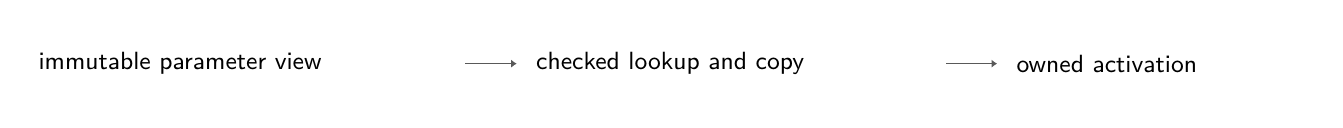
\begin{tikzpicture}[x=6.2pt,y=-13pt,draw=black!65,line width=.45pt]
\path[use as bounding box] (-1,-1) rectangle (74,1);
\draw (25,0) -- (24.5,0);
\draw (25,0) -- (25.5,0);
\draw (26,0) -- (25.5,0);
\draw (26,0) -- (26.5,0);
\draw[-{Latex[length=2pt,width=3pt]}] (26.5,0) -- (27.5,0);
\draw (53,0) -- (52.5,0);
\draw (53,0) -- (53.5,0);
\draw (54,0) -- (53.5,0);
\draw (54,0) -- (54.5,0);
\draw[-{Latex[length=2pt,width=3pt]}] (54.5,0) -- (55.5,0);
\node[anchor=west,inner sep=0pt,font=\sffamily\fontsize{9}{11}\selectfont] at (-0.4,0) {\begin{adjustbox}{max width=148.8pt}immutable parameter view\end{adjustbox}};
\node[anchor=west,inner sep=0pt,font=\sffamily\fontsize{9}{11}\selectfont] at (28.6,0) {\begin{adjustbox}{max width=142.6pt}checked lookup and copy\end{adjustbox}};
\node[anchor=west,inner sep=0pt,font=\sffamily\fontsize{9}{11}\selectfont] at (56.6,0) {\begin{adjustbox}{max width=99.2pt}owned activation\end{adjustbox}};
\end{tikzpicture}
\end{adjustbox}\end{center}

The fresh owner costs one read and one write per element. In the
simplest cold-payload accounting, a canonical \texttt{f32} lookup moves
approximately

\[
Q_{\mathrm{lookup}}\approx 8D\quad[\mathrm{bytes}],
\]

counting \(4D\) input bytes and \(4D\) output bytes. This is not
measured memory traffic: cache lines, write allocation, allocator
metadata, and warm data can change physical transfers. It is a useful
statement of the policy's payload cost.

In exchange, downstream mutation cannot alter \(\mathbf{E}\), the
activation can outlive the lookup borrow, and request cleanup has one
obvious owner. The
\href{https://github.com/hermonai/inside-the-llm-engine/blob/astra-visual-rewrite/diagrams/transformer/embedding-view-vs-copy.txt}{view-versus-copy
diagram} records both options rather than presenting the copy as free.

A database-table analogy can help for one moment: the embedding table is
long-lived storage, and an ID chooses a row. The analogy stops there.
These are learned numerical weights, not relational records; there is no
SQL predicate, transaction, schema evolution, or human field meaning.
The actual mechanism remains tensor indexing and copying.

\begin{quote}
\textbf{PROVE IT}
\href{https://github.com/hermonai/inside-the-llm-engine/blob/astra-visual-rewrite/labs/lab-32-embedding-view-vs-copy.md}{Lab
32} mutates the returned \texttt{OwnedTensor} and verifies that the
original table is unchanged. Ownership is tested behavior, not a
comment.
\end{quote}

\subsection{From one token to a
sequence}\label{from-one-token-to-a-sequence}

\begin{figure}[H]\centering\resizebox{\linewidth}{!}{% Generated from figures/generated/ch07-sequence.svg; do not hand edit.
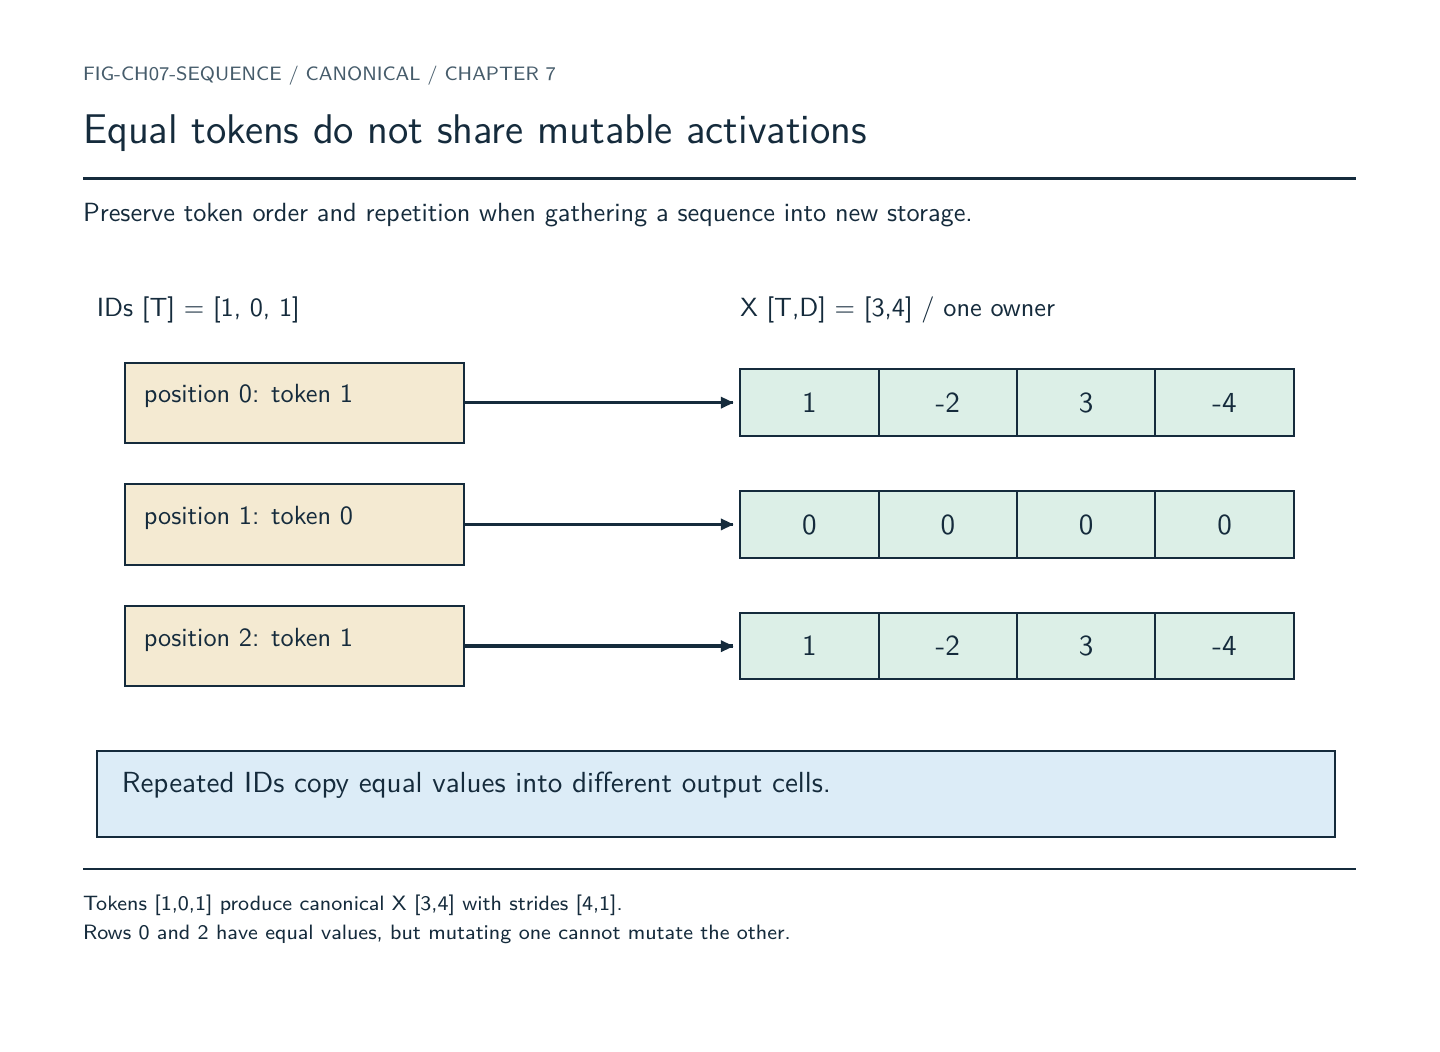
\begin{tikzpicture}[x=.5pt,y=-.5pt]
\path[use as bounding box] (0,0) rectangle (1000,720);
\path[fill=white,draw=none,line width=0.5pt] (0.0,0.0) rectangle (1000.0,720.0);
\node[inner sep=0pt,outer sep=0pt,anchor=base west,text={rgb,255:red,70;green,92;blue,107},font=\sffamily\fontsize{7.0}{8.4}\selectfont] at (40,38) {FIG-CH07-SEQUENCE  /  CANONICAL / CHAPTER 7};
\node[inner sep=0pt,outer sep=0pt,anchor=base west,text={rgb,255:red,21;green,43;blue,60},font=\sffamily\fontsize{15.0}{18.0}\selectfont] at (40,84) {Equal tokens do not share mutable activations};
\draw[fill=none,draw={rgb,255:red,21;green,43;blue,60},line width=0.75pt] (40,109) -- (960,109);
\node[inner sep=0pt,outer sep=0pt,anchor=base west,text={rgb,255:red,21;green,43;blue,60},font=\sffamily\fontsize{9.5}{11.4}\selectfont] at (40,140) {Preserve token order and repetition when gathering a sequence into new storage.};
\node[inner sep=0pt,outer sep=0pt,anchor=base west,text={rgb,255:red,21;green,43;blue,60},font=\sffamily\fontsize{9.5}{11.4}\selectfont] at (50,209) {IDs [T] = [1, 0, 1]};
\node[inner sep=0pt,outer sep=0pt,anchor=base west,text={rgb,255:red,21;green,43;blue,60},font=\sffamily\fontsize{9.5}{11.4}\selectfont] at (515,209) {X [T,D] = [3,4] / one owner};
\path[fill={rgb,255:red,244;green,234;blue,210},draw={rgb,255:red,21;green,43;blue,60},line width=0.7pt] (70.0,242.0) rectangle (315.0,300.0);
\node[inner sep=0pt,outer sep=0pt,anchor=base west,text={rgb,255:red,21;green,43;blue,60},font=\sffamily\fontsize{9.5}{11.4}\selectfont] at (84,271) {position 0: token 1};
\draw[fill=none,draw={rgb,255:red,21;green,43;blue,60},line width=1.25pt] (315,271) -- (510,271);
\path[fill={rgb,255:red,21;green,43;blue,60},draw=none,line width=0.5pt] (510.00,271.00) -- (501.00,275.35) -- (501.00,266.65) -- cycle;
\path[fill={rgb,255:red,220;green,239;blue,231},draw={rgb,255:red,21;green,43;blue,60},line width=0.7pt] (515.0,247.0) rectangle (615.0,295.0);
\node[inner sep=0pt,outer sep=0pt,anchor=base west,text={rgb,255:red,21;green,43;blue,60},font=\sffamily\fontsize{9.5}{11.4}\selectfont] at (529,276) {};
\node[inner sep=0pt,outer sep=0pt,anchor=base,text={rgb,255:red,21;green,43;blue,60},font=\sffamily\fontsize{10.5}{12.6}\selectfont] at (565.0,278) {1};
\path[fill={rgb,255:red,220;green,239;blue,231},draw={rgb,255:red,21;green,43;blue,60},line width=0.7pt] (615.0,247.0) rectangle (715.0,295.0);
\node[inner sep=0pt,outer sep=0pt,anchor=base west,text={rgb,255:red,21;green,43;blue,60},font=\sffamily\fontsize{9.5}{11.4}\selectfont] at (629,276) {};
\node[inner sep=0pt,outer sep=0pt,anchor=base,text={rgb,255:red,21;green,43;blue,60},font=\sffamily\fontsize{10.5}{12.6}\selectfont] at (665.0,278) {-2};
\path[fill={rgb,255:red,220;green,239;blue,231},draw={rgb,255:red,21;green,43;blue,60},line width=0.7pt] (715.0,247.0) rectangle (815.0,295.0);
\node[inner sep=0pt,outer sep=0pt,anchor=base west,text={rgb,255:red,21;green,43;blue,60},font=\sffamily\fontsize{9.5}{11.4}\selectfont] at (729,276) {};
\node[inner sep=0pt,outer sep=0pt,anchor=base,text={rgb,255:red,21;green,43;blue,60},font=\sffamily\fontsize{10.5}{12.6}\selectfont] at (765.0,278) {3};
\path[fill={rgb,255:red,220;green,239;blue,231},draw={rgb,255:red,21;green,43;blue,60},line width=0.7pt] (815.0,247.0) rectangle (915.0,295.0);
\node[inner sep=0pt,outer sep=0pt,anchor=base west,text={rgb,255:red,21;green,43;blue,60},font=\sffamily\fontsize{9.5}{11.4}\selectfont] at (829,276) {};
\node[inner sep=0pt,outer sep=0pt,anchor=base,text={rgb,255:red,21;green,43;blue,60},font=\sffamily\fontsize{10.5}{12.6}\selectfont] at (865.0,278) {-4};
\path[fill={rgb,255:red,244;green,234;blue,210},draw={rgb,255:red,21;green,43;blue,60},line width=0.7pt] (70.0,330.0) rectangle (315.0,388.0);
\node[inner sep=0pt,outer sep=0pt,anchor=base west,text={rgb,255:red,21;green,43;blue,60},font=\sffamily\fontsize{9.5}{11.4}\selectfont] at (84,359) {position 1: token 0};
\draw[fill=none,draw={rgb,255:red,21;green,43;blue,60},line width=1.25pt] (315,359) -- (510,359);
\path[fill={rgb,255:red,21;green,43;blue,60},draw=none,line width=0.5pt] (510.00,359.00) -- (501.00,363.35) -- (501.00,354.65) -- cycle;
\path[fill={rgb,255:red,220;green,239;blue,231},draw={rgb,255:red,21;green,43;blue,60},line width=0.7pt] (515.0,335.0) rectangle (615.0,383.0);
\node[inner sep=0pt,outer sep=0pt,anchor=base west,text={rgb,255:red,21;green,43;blue,60},font=\sffamily\fontsize{9.5}{11.4}\selectfont] at (529,364) {};
\node[inner sep=0pt,outer sep=0pt,anchor=base,text={rgb,255:red,21;green,43;blue,60},font=\sffamily\fontsize{10.5}{12.6}\selectfont] at (565.0,366) {0};
\path[fill={rgb,255:red,220;green,239;blue,231},draw={rgb,255:red,21;green,43;blue,60},line width=0.7pt] (615.0,335.0) rectangle (715.0,383.0);
\node[inner sep=0pt,outer sep=0pt,anchor=base west,text={rgb,255:red,21;green,43;blue,60},font=\sffamily\fontsize{9.5}{11.4}\selectfont] at (629,364) {};
\node[inner sep=0pt,outer sep=0pt,anchor=base,text={rgb,255:red,21;green,43;blue,60},font=\sffamily\fontsize{10.5}{12.6}\selectfont] at (665.0,366) {0};
\path[fill={rgb,255:red,220;green,239;blue,231},draw={rgb,255:red,21;green,43;blue,60},line width=0.7pt] (715.0,335.0) rectangle (815.0,383.0);
\node[inner sep=0pt,outer sep=0pt,anchor=base west,text={rgb,255:red,21;green,43;blue,60},font=\sffamily\fontsize{9.5}{11.4}\selectfont] at (729,364) {};
\node[inner sep=0pt,outer sep=0pt,anchor=base,text={rgb,255:red,21;green,43;blue,60},font=\sffamily\fontsize{10.5}{12.6}\selectfont] at (765.0,366) {0};
\path[fill={rgb,255:red,220;green,239;blue,231},draw={rgb,255:red,21;green,43;blue,60},line width=0.7pt] (815.0,335.0) rectangle (915.0,383.0);
\node[inner sep=0pt,outer sep=0pt,anchor=base west,text={rgb,255:red,21;green,43;blue,60},font=\sffamily\fontsize{9.5}{11.4}\selectfont] at (829,364) {};
\node[inner sep=0pt,outer sep=0pt,anchor=base,text={rgb,255:red,21;green,43;blue,60},font=\sffamily\fontsize{10.5}{12.6}\selectfont] at (865.0,366) {0};
\path[fill={rgb,255:red,244;green,234;blue,210},draw={rgb,255:red,21;green,43;blue,60},line width=0.7pt] (70.0,418.0) rectangle (315.0,476.0);
\node[inner sep=0pt,outer sep=0pt,anchor=base west,text={rgb,255:red,21;green,43;blue,60},font=\sffamily\fontsize{9.5}{11.4}\selectfont] at (84,447) {position 2: token 1};
\draw[fill=none,draw={rgb,255:red,21;green,43;blue,60},line width=1.25pt] (315,447) -- (510,447);
\path[fill={rgb,255:red,21;green,43;blue,60},draw=none,line width=0.5pt] (510.00,447.00) -- (501.00,451.35) -- (501.00,442.65) -- cycle;
\path[fill={rgb,255:red,220;green,239;blue,231},draw={rgb,255:red,21;green,43;blue,60},line width=0.7pt] (515.0,423.0) rectangle (615.0,471.0);
\node[inner sep=0pt,outer sep=0pt,anchor=base west,text={rgb,255:red,21;green,43;blue,60},font=\sffamily\fontsize{9.5}{11.4}\selectfont] at (529,452) {};
\node[inner sep=0pt,outer sep=0pt,anchor=base,text={rgb,255:red,21;green,43;blue,60},font=\sffamily\fontsize{10.5}{12.6}\selectfont] at (565.0,454) {1};
\path[fill={rgb,255:red,220;green,239;blue,231},draw={rgb,255:red,21;green,43;blue,60},line width=0.7pt] (615.0,423.0) rectangle (715.0,471.0);
\node[inner sep=0pt,outer sep=0pt,anchor=base west,text={rgb,255:red,21;green,43;blue,60},font=\sffamily\fontsize{9.5}{11.4}\selectfont] at (629,452) {};
\node[inner sep=0pt,outer sep=0pt,anchor=base,text={rgb,255:red,21;green,43;blue,60},font=\sffamily\fontsize{10.5}{12.6}\selectfont] at (665.0,454) {-2};
\path[fill={rgb,255:red,220;green,239;blue,231},draw={rgb,255:red,21;green,43;blue,60},line width=0.7pt] (715.0,423.0) rectangle (815.0,471.0);
\node[inner sep=0pt,outer sep=0pt,anchor=base west,text={rgb,255:red,21;green,43;blue,60},font=\sffamily\fontsize{9.5}{11.4}\selectfont] at (729,452) {};
\node[inner sep=0pt,outer sep=0pt,anchor=base,text={rgb,255:red,21;green,43;blue,60},font=\sffamily\fontsize{10.5}{12.6}\selectfont] at (765.0,454) {3};
\path[fill={rgb,255:red,220;green,239;blue,231},draw={rgb,255:red,21;green,43;blue,60},line width=0.7pt] (815.0,423.0) rectangle (915.0,471.0);
\node[inner sep=0pt,outer sep=0pt,anchor=base west,text={rgb,255:red,21;green,43;blue,60},font=\sffamily\fontsize{9.5}{11.4}\selectfont] at (829,452) {};
\node[inner sep=0pt,outer sep=0pt,anchor=base,text={rgb,255:red,21;green,43;blue,60},font=\sffamily\fontsize{10.5}{12.6}\selectfont] at (865.0,454) {-4};
\path[fill={rgb,255:red,220;green,236;blue,247},draw={rgb,255:red,21;green,43;blue,60},line width=0.7pt] (50.0,523.0) rectangle (945.0,585.0);
\node[inner sep=0pt,outer sep=0pt,anchor=base west,text={rgb,255:red,21;green,43;blue,60},font=\sffamily\fontsize{9.5}{11.4}\selectfont] at (64,552) {};
\node[inner sep=0pt,outer sep=0pt,anchor=base west,text={rgb,255:red,21;green,43;blue,60},font=\sffamily\fontsize{10.5}{12.6}\selectfont] at (68,553) {Repeated IDs copy equal values into different output cells.};
\draw[fill=none,draw={rgb,255:red,21;green,43;blue,60},line width=0.75pt] (40,608) -- (960,608);
\node[inner sep=0pt,outer sep=0pt,anchor=base west,text={rgb,255:red,21;green,43;blue,60},font=\sffamily\fontsize{7.5}{9.0}\selectfont] at (40,638) {Tokens [1,0,1] produce canonical X [3,4] with strides [4,1].};
\node[inner sep=0pt,outer sep=0pt,anchor=base west,text={rgb,255:red,21;green,43;blue,60},font=\sffamily\fontsize{7.5}{9.0}\selectfont] at (40,659) {Rows 0 and 2 have equal values, but mutating one cannot mutate the other.};
\end{tikzpicture}
}\caption{Repeated token identities produce equal rows at distinct positions in one activation allocation.}\end{figure}

Positions and identities are separate axes of reasoning. Positions 0 and
2 can contain the same token ID without sharing mutable output cells. In
this fixture, changing \texttt{X{[}0,0{]}} cannot change
\texttt{X{[}2,0{]}}, even though lookup originally wrote the same value
into both. An optimization that deduplicated parameter reads would still
owe the same logical output and ownership contract.

Inference begins with more than one prompt token even though later
generation produces one new token at a time. The single-row rule
generalizes without introducing attention.

For the token sequence

\[
\mathbf{t}=[t_0,t_1,\ldots,t_{T-1}],
\]

sequence embedding produces

\[
\mathbf{X}\in\mathbb{R}^{T\times D},
\qquad X_{ij}=E_{t_i,j},
\]

for \(0\le i<T\) and \(0\le j<D\). The shapes are:

\begin{verbatim}
token identities   [T]
embedding table    [V,D]
result             [T,D]
\end{verbatim}

\texttt{\seqsplit{embedding\_sequence\_reference}} validates the same
positive table dimensions, checks prospective output element count
\(TD\), then checks each token before copying its logical row. It
preserves order and repetition. Tokens \texttt{{[}3,0,3{]}} produce rows
\texttt{{[}E3,E0,E3{]}}; it does not deduplicate them or sort for
locality.

An empty token sequence has \(T=0\) and returns an owned tensor with
shape \texttt{{[}0,D{]}}. That result has a well-defined shape and no
values. This does not make an empty model vocabulary valid: \(V=0\)
leaves no token identity selectable, and \(D=0\) would not create a
model-space vector. The axes have independent contracts.

The implementation is intentionally only a gather into
\texttt{{[}T,D{]}}. It does not create batches, positions, masks, Q/K/V,
or a Transformer block. Those concepts need separate semantic and
ownership work.

\subsection{The residual-stream
invariant}\label{the-residual-stream-invariant}

\begin{figure}[H]\centering\resizebox{\linewidth}{!}{% Generated from figures/generated/ch07-owners.svg; do not hand edit.
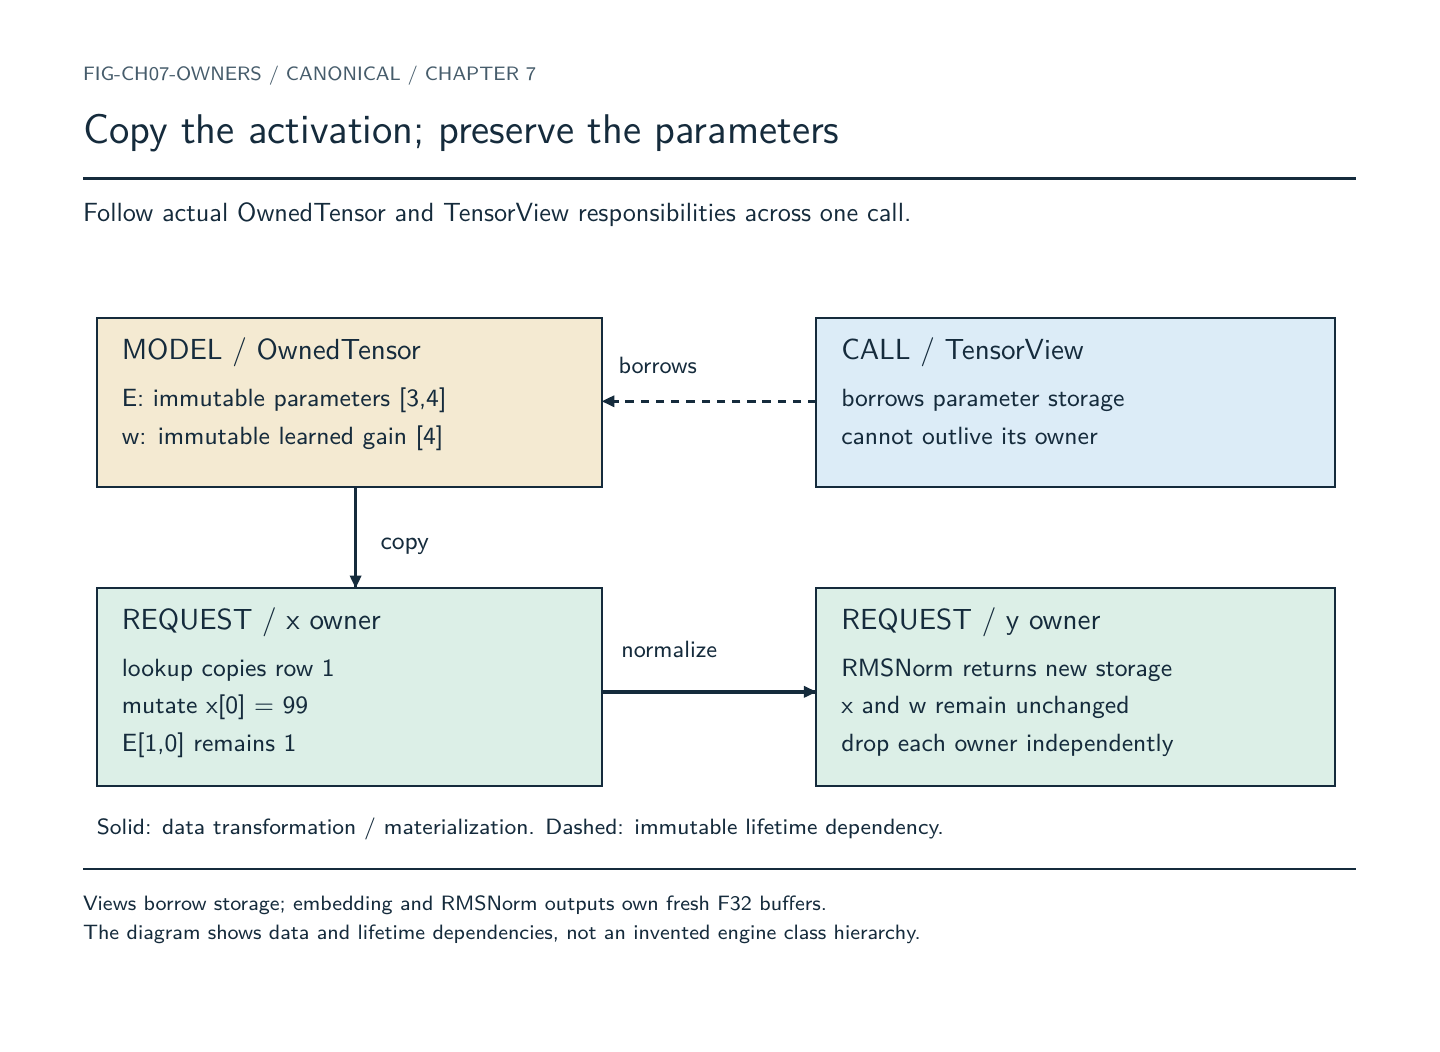
\begin{tikzpicture}[x=.5pt,y=-.5pt]
\path[use as bounding box] (0,0) rectangle (1000,720);
\path[fill=white,draw=none,line width=0.5pt] (0.0,0.0) rectangle (1000.0,720.0);
\node[inner sep=0pt,outer sep=0pt,anchor=base west,text={rgb,255:red,70;green,92;blue,107},font=\sffamily\fontsize{7.0}{8.4}\selectfont] at (40,38) {FIG-CH07-OWNERS  /  CANONICAL / CHAPTER 7};
\node[inner sep=0pt,outer sep=0pt,anchor=base west,text={rgb,255:red,21;green,43;blue,60},font=\sffamily\fontsize{15.0}{18.0}\selectfont] at (40,84) {Copy the activation; preserve the parameters};
\draw[fill=none,draw={rgb,255:red,21;green,43;blue,60},line width=0.75pt] (40,109) -- (960,109);
\node[inner sep=0pt,outer sep=0pt,anchor=base west,text={rgb,255:red,21;green,43;blue,60},font=\sffamily\fontsize{9.5}{11.4}\selectfont] at (40,140) {Follow actual OwnedTensor and TensorView responsibilities across one call.};
\path[fill={rgb,255:red,244;green,234;blue,210},draw={rgb,255:red,21;green,43;blue,60},line width=0.7pt] (50.0,210.0) rectangle (415.0,332.0);
\node[inner sep=0pt,outer sep=0pt,anchor=base west,text={rgb,255:red,21;green,43;blue,60},font=\sffamily\fontsize{9.5}{11.4}\selectfont] at (64,239) {};
\node[inner sep=0pt,outer sep=0pt,anchor=base west,text={rgb,255:red,21;green,43;blue,60},font=\sffamily\fontsize{10.5}{12.6}\selectfont] at (68,240) {MODEL / OwnedTensor};
\node[inner sep=0pt,outer sep=0pt,anchor=base west,text={rgb,255:red,21;green,43;blue,60},font=\sffamily\fontsize{9.0}{10.799999999999999}\selectfont] at (68,274) {E: immutable parameters [3,4]};
\node[inner sep=0pt,outer sep=0pt,anchor=base west,text={rgb,255:red,21;green,43;blue,60},font=\sffamily\fontsize{9.0}{10.799999999999999}\selectfont] at (68,301) {w: immutable learned gain [4]};
\path[fill={rgb,255:red,220;green,236;blue,247},draw={rgb,255:red,21;green,43;blue,60},line width=0.7pt] (570.0,210.0) rectangle (945.0,332.0);
\node[inner sep=0pt,outer sep=0pt,anchor=base west,text={rgb,255:red,21;green,43;blue,60},font=\sffamily\fontsize{9.5}{11.4}\selectfont] at (584,239) {};
\node[inner sep=0pt,outer sep=0pt,anchor=base west,text={rgb,255:red,21;green,43;blue,60},font=\sffamily\fontsize{10.5}{12.6}\selectfont] at (588,240) {CALL / TensorView};
\node[inner sep=0pt,outer sep=0pt,anchor=base west,text={rgb,255:red,21;green,43;blue,60},font=\sffamily\fontsize{9.0}{10.799999999999999}\selectfont] at (588,274) {borrows parameter storage};
\node[inner sep=0pt,outer sep=0pt,anchor=base west,text={rgb,255:red,21;green,43;blue,60},font=\sffamily\fontsize{9.0}{10.799999999999999}\selectfont] at (588,301) {cannot outlive its owner};
\draw[fill=none,draw={rgb,255:red,21;green,43;blue,60},line width=1.25pt,dash pattern=on 3.0pt off 2.5pt] (570,270) -- (415,270);
\path[fill={rgb,255:red,21;green,43;blue,60},draw=none,line width=0.5pt] (415.00,270.00) -- (424.00,265.65) -- (424.00,274.35) -- cycle;
\node[inner sep=0pt,outer sep=0pt,anchor=base west,text={rgb,255:red,21;green,43;blue,60},font=\sffamily\fontsize{8.5}{10.2}\selectfont] at (427,250) {borrows};
\path[fill={rgb,255:red,220;green,239;blue,231},draw={rgb,255:red,21;green,43;blue,60},line width=0.7pt] (50.0,405.0) rectangle (415.0,548.0);
\node[inner sep=0pt,outer sep=0pt,anchor=base west,text={rgb,255:red,21;green,43;blue,60},font=\sffamily\fontsize{9.5}{11.4}\selectfont] at (64,434) {};
\node[inner sep=0pt,outer sep=0pt,anchor=base west,text={rgb,255:red,21;green,43;blue,60},font=\sffamily\fontsize{10.5}{12.6}\selectfont] at (68,435) {REQUEST / x owner};
\node[inner sep=0pt,outer sep=0pt,anchor=base west,text={rgb,255:red,21;green,43;blue,60},font=\sffamily\fontsize{9.0}{10.799999999999999}\selectfont] at (68,469) {lookup copies row 1};
\node[inner sep=0pt,outer sep=0pt,anchor=base west,text={rgb,255:red,21;green,43;blue,60},font=\sffamily\fontsize{9.0}{10.799999999999999}\selectfont] at (68,496) {mutate x[0] = 99};
\node[inner sep=0pt,outer sep=0pt,anchor=base west,text={rgb,255:red,21;green,43;blue,60},font=\sffamily\fontsize{9.0}{10.799999999999999}\selectfont] at (68,523) {E[1,0] remains 1};
\path[fill={rgb,255:red,220;green,239;blue,231},draw={rgb,255:red,21;green,43;blue,60},line width=0.7pt] (570.0,405.0) rectangle (945.0,548.0);
\node[inner sep=0pt,outer sep=0pt,anchor=base west,text={rgb,255:red,21;green,43;blue,60},font=\sffamily\fontsize{9.5}{11.4}\selectfont] at (584,434) {};
\node[inner sep=0pt,outer sep=0pt,anchor=base west,text={rgb,255:red,21;green,43;blue,60},font=\sffamily\fontsize{10.5}{12.6}\selectfont] at (588,435) {REQUEST / y owner};
\node[inner sep=0pt,outer sep=0pt,anchor=base west,text={rgb,255:red,21;green,43;blue,60},font=\sffamily\fontsize{9.0}{10.799999999999999}\selectfont] at (588,469) {RMSNorm returns new storage};
\node[inner sep=0pt,outer sep=0pt,anchor=base west,text={rgb,255:red,21;green,43;blue,60},font=\sffamily\fontsize{9.0}{10.799999999999999}\selectfont] at (588,496) {x and w remain unchanged};
\node[inner sep=0pt,outer sep=0pt,anchor=base west,text={rgb,255:red,21;green,43;blue,60},font=\sffamily\fontsize{9.0}{10.799999999999999}\selectfont] at (588,523) {drop each owner independently};
\draw[fill=none,draw={rgb,255:red,21;green,43;blue,60},line width=1.25pt] (237,332) -- (237,405);
\path[fill={rgb,255:red,21;green,43;blue,60},draw=none,line width=0.5pt] (237.00,405.00) -- (232.65,396.00) -- (241.35,396.00) -- cycle;
\node[inner sep=0pt,outer sep=0pt,anchor=base west,text={rgb,255:red,21;green,43;blue,60},font=\sffamily\fontsize{9.0}{10.799999999999999}\selectfont] at (255,377) {copy};
\draw[fill=none,draw={rgb,255:red,21;green,43;blue,60},line width=1.25pt] (415,480) -- (570,480);
\path[fill={rgb,255:red,21;green,43;blue,60},draw=none,line width=0.5pt] (570.00,480.00) -- (561.00,484.35) -- (561.00,475.65) -- cycle;
\node[inner sep=0pt,outer sep=0pt,anchor=base west,text={rgb,255:red,21;green,43;blue,60},font=\sffamily\fontsize{8.5}{10.2}\selectfont] at (429,455) {normalize};
\node[inner sep=0pt,outer sep=0pt,anchor=base west,text={rgb,255:red,21;green,43;blue,60},font=\sffamily\fontsize{8.0}{9.6}\selectfont] at (50,583) {Solid: data transformation / materialization. Dashed: immutable lifetime dependency.};
\draw[fill=none,draw={rgb,255:red,21;green,43;blue,60},line width=0.75pt] (40,608) -- (960,608);
\node[inner sep=0pt,outer sep=0pt,anchor=base west,text={rgb,255:red,21;green,43;blue,60},font=\sffamily\fontsize{7.5}{9.0}\selectfont] at (40,638) {Views borrow storage; embedding and RMSNorm outputs own fresh F32 buffers.};
\node[inner sep=0pt,outer sep=0pt,anchor=base west,text={rgb,255:red,21;green,43;blue,60},font=\sffamily\fontsize{7.5}{9.0}\selectfont] at (40,659) {The diagram shows data and lifetime dependencies, not an invented engine class hierarchy.};
\end{tikzpicture}
}\caption{Model parameters, immutable views and request-owned activation tensors have distinct lifetimes.}\end{figure}

This diagram uses the real storage types, \texttt{OwnedTensor} and
\texttt{TensorView}, not an imagined Transformer class hierarchy. The
dashed edge points from a view to the owner it borrows. Solid edges
represent a copy or numerical transformation. Neither means transferring
ownership of model weights into a request. Model storage can serve many
requests; request cleanup must release only its own activation owners.

Once lookup produces \(\mathbf{x}_0\in\mathbb{R}^{D}\) for a token,
\(D\) becomes one of the decoder's central dimensional invariants.
Transformer sublayers can create internal tensors with other shapes, but
a value added back into the residual stream must return to model width
\(D\).

The
\href{https://github.com/hermonai/inside-the-llm-engine/blob/astra-visual-rewrite/diagrams/transformer/residual-stream-width.txt}{residual-width
diagram} states that bounded claim. ``Persistent'' means the state is
carried through the layer sequence for this request, not that it has
model lifetime or durable storage. It is activation data. The embedding
table and normalization weights are parameters; the residual vectors are
request-owned values.

This distinction is summarized in the
\href{https://github.com/hermonai/inside-the-llm-engine/blob/astra-visual-rewrite/diagrams/transformer/parameters-vs-activations.txt}{parameter/activation
diagram}:

\begin{center}\begin{adjustbox}{max width=\linewidth}% Legacy topology preserved as native vectors and typeset labels.
\begin{tikzpicture}[x=6.2pt,y=-13pt,draw=black!65,line width=.45pt]
\path[use as bounding box] (-1,-1) rectangle (58,3);
\node[anchor=west,inner sep=0pt,font=\sffamily\fontsize{9}{11}\selectfont] at (-0.4,0) {\begin{adjustbox}{max width=86.8pt}MODEL LIFETIME\end{adjustbox}};
\node[anchor=west,inner sep=0pt,font=\sffamily\fontsize{9}{11}\selectfont] at (39.6,0) {\begin{adjustbox}{max width=99.2pt}REQUEST LIFETIME\end{adjustbox}};
\draw (20,1) -- (19.5,1);
\draw (20,1) -- (20.5,1);
\draw (21,1) -- (20.5,1);
\draw (21,1) -- (21.5,1);
\draw (33,1) -- (32.5,1);
\draw (33,1) -- (33.5,1);
\draw (34,1) -- (33.5,1);
\draw (34,1) -- (34.5,1);
\draw[-{Latex[length=2pt,width=3pt]}] (34.5,1) -- (35.5,1);
\node[anchor=west,inner sep=0pt,font=\sffamily\fontsize{9}{11}\selectfont] at (-0.4,1) {\begin{adjustbox}{max width=117.8pt}(embedding E [V,D])\end{adjustbox}};
\node[anchor=west,inner sep=0pt,font=\sffamily\fontsize{9}{11}\selectfont] at (22.6,1) {\begin{adjustbox}{max width=55.800000000000004pt}read/copy\end{adjustbox}};
\node[anchor=west,inner sep=0pt,font=\sffamily\fontsize{9}{11}\selectfont] at (38.6,1) {\begin{adjustbox}{max width=99.2pt}[residual x [D]]\end{adjustbox}};
\draw (16,2) -- (15.5,2);
\draw (16,2) -- (16.5,2);
\draw (17,2) -- (16.5,2);
\draw (17,2) -- (17.5,2);
\draw (18,2) -- (17.5,2);
\draw (18,2) -- (18.5,2);
\draw (19,2) -- (18.5,2);
\draw (19,2) -- (19.5,2);
\draw (20,2) -- (19.5,2);
\draw (20,2) -- (20.5,2);
\draw (21,2) -- (20.5,2);
\draw (21,2) -- (21.5,2);
\draw (28,2) -- (27.5,2);
\draw (28,2) -- (28.5,2);
\draw (29,2) -- (28.5,2);
\draw (29,2) -- (29.5,2);
\draw (30,2) -- (29.5,2);
\draw (30,2) -- (30.5,2);
\draw (31,2) -- (30.5,2);
\draw (31,2) -- (31.5,2);
\draw (32,2) -- (31.5,2);
\draw (32,2) -- (32.5,2);
\draw (33,2) -- (32.5,2);
\draw (33,2) -- (33.5,2);
\draw (34,2) -- (33.5,2);
\draw (34,2) -- (34.5,2);
\draw[-{Latex[length=2pt,width=3pt]}] (34.5,2) -- (35.5,2);
\node[anchor=west,inner sep=0pt,font=\sffamily\fontsize{9}{11}\selectfont] at (-0.4,2) {\begin{adjustbox}{max width=93.0pt}(RMSNorm w [D])\end{adjustbox}};
\node[anchor=west,inner sep=0pt,font=\sffamily\fontsize{9}{11}\selectfont] at (22.6,2) {\begin{adjustbox}{max width=24.8pt}read\end{adjustbox}};
\node[anchor=west,inner sep=0pt,font=\sffamily\fontsize{9}{11}\selectfont] at (38.6,2) {\begin{adjustbox}{max width=111.60000000000001pt}[normalized y [D]]\end{adjustbox}};
\end{tikzpicture}
\end{adjustbox}\end{center}

Inference does not update the learned parameters. Multiple requests may
read them concurrently. Each request owns the activations it creates and
eventually releases them. Later chapters will give that distinction
consequences for loading, placement, caches, and scheduling; here it
already prevents parameter aliasing.

\subsection{Why scale needs a
contract}\label{why-scale-needs-a-contract}

Consider two vectors:

\[
\mathbf{x}_1=[1,2,-1,2],
\qquad
\mathbf{x}_2=[10,20,-10,20].
\]

The second is \(10\mathbf{x}_1\). Their coordinate pattern and direction
agree, but every component of the second is ten times larger. Repeated
learned transformations and residual additions can produce activation
scales that vary across layers and inputs. Later matrix products
multiply those values by many weights, so scale affects representable
range and numerical behavior.

Normalization provides a defined rescaling based on a vector statistic.
It is not clipping. A clipping operator might independently replace
every value above a threshold with that threshold, changing coordinates
selectively. RMSNorm computes one scalar from the entire vector, scales
every coordinate by that shared value, and then applies learned
per-coordinate weights. Large components remain large relative to small
components unless learned scale changes that relation.

The original RMSNorm paper by Biao Zhang and Rico Sennrich proposed
removing LayerNorm's recentering step while retaining RMS-based
rescaling. That history is useful, but the inference engine still needs
the exact forward equation.

\subsection{Root mean square from first
principles}\label{root-mean-square-from-first-principles}

Let

\[
\mathbf{x}=[x_0,x_1,\ldots,x_{D-1}]\in\mathbb{R}^{D},
\qquad D>0.
\]

First square each component. Squaring makes every contribution
nonnegative, so opposite signs cannot cancel. Next take the arithmetic
mean:

\[
m_2(\mathbf{x})=\frac{1}{D}\sum_{i=0}^{D-1}x_i^2.
\]

The quantity \(m_2\) has squared units relative to \(\mathbf{x}\).
Taking the square root restores the original units:

\[
\operatorname{RMS}(\mathbf{x})
=\sqrt{\frac{1}{D}\sum_{i=0}^{D-1}x_i^2}.
\]

That sequence---square, mean, root---is the name \textbf{root mean
square}. The
\href{https://github.com/hermonai/inside-the-llm-engine/blob/astra-visual-rewrite/diagrams/transformer/rms-calculation-pipeline.txt}{RMS
pipeline} makes each lowering step visible.

Why take a mean rather than only a sum? If a vector repeated the same
magnitude at every coordinate, the sum of squares would grow with \(D\).
Dividing by \(D\) makes its RMS equal that coordinate magnitude,
independent of vector length. For \texttt{{[}4,4,4,4{]}}, RMS is 4, not
8.

RMS alone has a zero-denominator problem. For the zero vector, every
square and their mean are zero. The reciprocal required for
normalization would be undefined. RMSNorm therefore defines an
epsilon-stabilized denominator. In this book and the checked operator,
epsilon is \emph{inside} the square root:

\[
r=\frac{1}{\sqrt{m_2(\mathbf{x})+\epsilon}},
\qquad \epsilon>0.
\]

The expression

\[
\frac{1}{\sqrt{m_2(\mathbf{x})}+\epsilon}
\]

is a different function. It cannot be substituted just because both
contain a square root and epsilon. PyTorch's official RMSNorm semantics
and the inspected Hermon/llama.cpp paths use the first convention.

\subsection{The RMSNorm operator}\label{the-rmsnorm-operator}

RMS rescaling alone would apply scalar \(r\) to every coordinate.
RMSNorm also has a learned scale vector

\[
\mathbf{w}\in\mathbb{R}^{D}.
\]

The complete operator is

\[
\boxed{
y_i=x_i
\left(
\frac{1}{\sqrt{\frac{1}{D}\sum_{j=0}^{D-1}x_j^2+\epsilon}}
\right)
w_i
},
\qquad 0\le i<D.
\]

Equivalently, if \(r\) names the scalar reciprocal RMS,

\[
\mathbf{y}=r(\mathbf{x}\odot\mathbf{w}),
\qquad
\mathbf{x},\mathbf{w},\mathbf{y}\in\mathbb{R}^{D}.
\]

The operator has two different kinds of multiplication. The reciprocal
RMS \(r\) is one scalar derived from all of \(\mathbf{x}\). The learned
scale \(\mathbf{w}\) is element-wise: coordinate \(i\) uses \(w_i\). The
symbol \(\odot\) denotes that element-wise product, not a dot product.

Learned scale lets the trained model adjust normalized coordinates
instead of forcing every feature to use identical output scale. During
inference, \(\mathbf{w}\) is immutable parameter data. No learning
occurs inside this function.

\Needspace{28\baselineskip}

\subsubsection{A complete calculation by
hand}\label{a-complete-calculation-by-hand}

Use

\[
\mathbf{x}=[1,-2,3,-4],\qquad
\mathbf{w}=[1,0.5,2,-1],\qquad
\epsilon=10^{-5}.
\]

The squares sum to

\[
1^2+(-2)^2+3^2+(-4)^2=1+4+9+16=30.
\]

With \(D=4\),

\[
m_2=\frac{30}{4}=7.5,
\]

and

\[
r=\frac{1}{\sqrt{7.5+10^{-5}}}
\approx0.36514813.
\]

Applying both scales gives

\[
\begin{aligned}
y_0&= 1(r)(1)       &&\approx 0.36514813,\\
y_1&=-2(r)(0.5)     &&\approx-0.36514813,\\
y_2&= 3(r)(2)       &&\approx 2.1908888,\\
y_3&=-4(r)(-1)      &&\approx 1.4605925.
\end{aligned}
\]

The independent Python oracle and a focused Rust test calculate the
entire vector. The printed decimals are evidence from those programs,
not unchecked mental arithmetic.

\begin{quote}
\textbf{BUILD IT} Complete
\href{https://github.com/hermonai/inside-the-llm-engine/blob/astra-visual-rewrite/labs/lab-33-compute-rms-by-hand.md}{Lab
33}. Keep exact symbolic steps separate from approximate decimal output,
then use
\href{https://github.com/hermonai/inside-the-llm-engine/blob/astra-visual-rewrite/labs/lab-34-implement-rmsnorm.md}{Lab
34} to trace those same stages through the reference operator.
\end{quote}

\subsection{Equation to two loops}\label{equation-to-two-loops}

\begin{figure}[H]\centering\resizebox{\linewidth}{!}{% Generated from figures/generated/ch07-passes.svg; do not hand edit.
\begin{tikzpicture}[x=.5pt,y=-.5pt]
\path[use as bounding box] (0,0) rectangle (1000,720);
\path[fill=white,draw=none,line width=0.5pt] (0.0,0.0) rectangle (1000.0,720.0);
\node[inner sep=0pt,outer sep=0pt,anchor=base west,text={rgb,255:red,70;green,92;blue,107},font=\sffamily\fontsize{7.0}{8.4}\selectfont] at (40,38) {FIG-CH07-PASSES  /  CANONICAL / CHAPTER 7};
\node[inner sep=0pt,outer sep=0pt,anchor=base west,text={rgb,255:red,21;green,43;blue,60},font=\sffamily\fontsize{15.0}{18.0}\selectfont] at (40,84) {One reduction, then four output coordinates};
\draw[fill=none,draw={rgb,255:red,21;green,43;blue,60},line width=0.75pt] (40,109) -- (960,109);
\node[inner sep=0pt,outer sep=0pt,anchor=base west,text={rgb,255:red,21;green,43;blue,60},font=\sffamily\fontsize{9.5}{11.4}\selectfont] at (40,140) {Follow every square and partial sum before broadcasting the reciprocal RMS.};
\node[inner sep=0pt,outer sep=0pt,anchor=base west,text={rgb,255:red,21;green,43;blue,60},font=\sffamily\fontsize{10.0}{12.0}\selectfont] at (50,207) {PASS 1 / read all x before producing any y};
\path[fill={rgb,255:red,220;green,236;blue,247},draw={rgb,255:red,21;green,43;blue,60},line width=0.7pt] (50.0,231.0) rectangle (480.0,380.0);
\node[inner sep=0pt,outer sep=0pt,anchor=base west,text={rgb,255:red,21;green,43;blue,60},font=\sffamily\fontsize{9.5}{11.4}\selectfont] at (64,260) {};
\node[inner sep=0pt,outer sep=0pt,anchor=base west,text={rgb,255:red,21;green,43;blue,60},font=\sffamily\fontsize{10.5}{12.6}\selectfont] at (68,261) {01 / Square};
\node[inner sep=0pt,outer sep=0pt,anchor=base west,text={rgb,255:red,21;green,43;blue,60},font=\sffamily\fontsize{9.0}{10.799999999999999}\selectfont] at (68,295) {x = [1, -2, 3, -4]};
\node[inner sep=0pt,outer sep=0pt,anchor=base west,text={rgb,255:red,21;green,43;blue,60},font=\sffamily\fontsize{9.0}{10.799999999999999}\selectfont] at (68,322) {x² = [1, 4, 9, 16]};
\path[fill={rgb,255:red,220;green,236;blue,247},draw={rgb,255:red,21;green,43;blue,60},line width=0.7pt] (515.0,231.0) rectangle (945.0,380.0);
\node[inner sep=0pt,outer sep=0pt,anchor=base west,text={rgb,255:red,21;green,43;blue,60},font=\sffamily\fontsize{9.5}{11.4}\selectfont] at (529,260) {};
\node[inner sep=0pt,outer sep=0pt,anchor=base west,text={rgb,255:red,21;green,43;blue,60},font=\sffamily\fontsize{10.5}{12.6}\selectfont] at (533,261) {02 / Reduce};
\node[inner sep=0pt,outer sep=0pt,anchor=base west,text={rgb,255:red,21;green,43;blue,60},font=\sffamily\fontsize{9.0}{10.799999999999999}\selectfont] at (533,295) {partial sums = [1, 5, 14, 30]};
\node[inner sep=0pt,outer sep=0pt,anchor=base west,text={rgb,255:red,21;green,43;blue,60},font=\sffamily\fontsize{9.0}{10.799999999999999}\selectfont] at (533,322) {mean = 30 / 4 = 7.5};
\path[fill={rgb,255:red,220;green,236;blue,247},draw={rgb,255:red,21;green,43;blue,60},line width=0.7pt] (50.0,404.0) rectangle (480.0,553.0);
\node[inner sep=0pt,outer sep=0pt,anchor=base west,text={rgb,255:red,21;green,43;blue,60},font=\sffamily\fontsize{9.5}{11.4}\selectfont] at (64,433) {};
\node[inner sep=0pt,outer sep=0pt,anchor=base west,text={rgb,255:red,21;green,43;blue,60},font=\sffamily\fontsize{10.5}{12.6}\selectfont] at (68,434) {03 / Reciprocal RMS};
\node[inner sep=0pt,outer sep=0pt,anchor=base west,text={rgb,255:red,21;green,43;blue,60},font=\sffamily\fontsize{9.0}{10.799999999999999}\selectfont] at (68,468) {epsilon = 0.00001};
\node[inner sep=0pt,outer sep=0pt,anchor=base west,text={rgb,255:red,21;green,43;blue,60},font=\sffamily\fontsize{9.0}{10.799999999999999}\selectfont] at (68,495) {r = 1 / √(7.5 + epsilon)};
\node[inner sep=0pt,outer sep=0pt,anchor=base west,text={rgb,255:red,21;green,43;blue,60},font=\sffamily\fontsize{9.0}{10.799999999999999}\selectfont] at (68,522) {r ≈ 0.365148};
\path[fill={rgb,255:red,220;green,236;blue,247},draw={rgb,255:red,21;green,43;blue,60},line width=0.7pt] (515.0,404.0) rectangle (945.0,553.0);
\node[inner sep=0pt,outer sep=0pt,anchor=base west,text={rgb,255:red,21;green,43;blue,60},font=\sffamily\fontsize{9.5}{11.4}\selectfont] at (529,433) {};
\node[inner sep=0pt,outer sep=0pt,anchor=base west,text={rgb,255:red,21;green,43;blue,60},font=\sffamily\fontsize{10.5}{12.6}\selectfont] at (533,434) {04 / Scale and write};
\node[inner sep=0pt,outer sep=0pt,anchor=base west,text={rgb,255:red,21;green,43;blue,60},font=\sffamily\fontsize{9.0}{10.799999999999999}\selectfont] at (533,468) {PASS 2 / read x and w};
\node[inner sep=0pt,outer sep=0pt,anchor=base west,text={rgb,255:red,21;green,43;blue,60},font=\sffamily\fontsize{9.0}{10.799999999999999}\selectfont] at (533,495) {w = [1, 0.5, 2, -1]};
\node[inner sep=0pt,outer sep=0pt,anchor=base west,text={rgb,255:red,21;green,43;blue,60},font=\sffamily\fontsize{9.0}{10.799999999999999}\selectfont] at (533,522) {yᵢ = (xᵢ × r) × wᵢ};
\draw[fill=none,draw={rgb,255:red,21;green,43;blue,60},line width=1.25pt] (480,304) -- (515,304);
\path[fill={rgb,255:red,21;green,43;blue,60},draw=none,line width=0.5pt] (515.00,304.00) -- (506.00,308.35) -- (506.00,299.65) -- cycle;
\draw[fill=none,draw={rgb,255:red,21;green,43;blue,60},line width=0.75pt] (730,380) -- (730,392);
\draw[fill=none,draw={rgb,255:red,21;green,43;blue,60},line width=0.75pt] (730,392) -- (260,392);
\draw[fill=none,draw={rgb,255:red,21;green,43;blue,60},line width=1.25pt] (260,392) -- (260,404);
\path[fill={rgb,255:red,21;green,43;blue,60},draw=none,line width=0.5pt] (260.00,404.00) -- (255.65,395.00) -- (264.35,395.00) -- cycle;
\draw[fill=none,draw={rgb,255:red,21;green,43;blue,60},line width=1.25pt] (480,478) -- (515,478);
\path[fill={rgb,255:red,21;green,43;blue,60},draw=none,line width=0.5pt] (515.00,478.00) -- (506.00,482.35) -- (506.00,473.65) -- cycle;
\node[inner sep=0pt,outer sep=0pt,anchor=base west,text={rgb,255:red,21;green,43;blue,60},font=\sffamily\fontsize{8.5}{10.2}\selectfont] at (50,589) {The shared denominator includes x[3]; y[0] cannot be finalized after reading only x[0].};
\draw[fill=none,draw={rgb,255:red,21;green,43;blue,60},line width=0.75pt] (40,608) -- (960,608);
\node[inner sep=0pt,outer sep=0pt,anchor=base west,text={rgb,255:red,21;green,43;blue,60},font=\sffamily\fontsize{7.5}{9.0}\selectfont] at (40,638) {x [4] and learned w [4] are immutable; epsilon = 1e-5 is inside the root.};
\node[inner sep=0pt,outer sep=0pt,anchor=base west,text={rgb,255:red,21;green,43;blue,60},font=\sffamily\fontsize{7.5}{9.0}\selectfont] at (40,659) {Products, sums and output are F32; y [4] has canonical owned storage.};
\end{tikzpicture}
}\caption{Four squares reduce to a shared reciprocal RMS before the second pass writes output coordinates.}\end{figure}

The
\href{https://github.com/hermonai/inside-the-llm-engine/blob/astra-visual-rewrite/figures/generated/ch07-passes.html}{four-step
sequence} highlights the same stages, with keyboard controls and no
autoplay. Its static plate is complete: every intermediate needed for
the hand calculation remains visible in print. The highlighted stage
changes only the explanation, not the reduction order. Partial sums
\texttt{{[}1,5,14,30{]}} correspond to increasing logical index, exactly
as the reference loop below.

The direct lowering naturally has two logical passes:

\begin{verbatim}
sum_squares = 0
for i in 0..D:
    sum_squares += x[i] * x[i]

mean_square = sum_squares / D
inverse_rms = 1 / sqrt(mean_square + epsilon)

for i in 0..D:
    y[i] = x[i] * inverse_rms * weight[i]
\end{verbatim}

Pass one reduces \(D\) values to the scalar \(r\). Pass two broadcasts
that scalar while reading the input again and reading learned weights.
The output for coordinate zero cannot be finalized before pass one has
seen the last input, because the last square contributes to its
denominator.

The
\href{https://github.com/hermonai/inside-the-llm-engine/blob/astra-visual-rewrite/diagrams/transformer/rmsnorm-two-pass.txt}{two-pass
diagram} follows the data, and the
\href{https://github.com/hermonai/inside-the-llm-engine/blob/astra-visual-rewrite/diagrams/transformer/equation-to-loop.txt}{equation-to-loop
diagram} connects symbols, tensor shapes, checked logical indices, and
execution. The reference implementation follows it closely:

\Needspace{20\baselineskip}

\begin{verbatim}
let mut sum_squares = 0.0_f32;
for index in 0..dimension {
    let value = *input.get(&[index])?;
    let square = value * value;
    sum_squares += square;
}

let mean_square = sum_squares / dimension as f32;
let inverse_rms = 1.0_f32 / (mean_square + epsilon).sqrt();

for index in 0..dimension {
    output.push(*input.get(&[index])? * inverse_rms * *weight.get(&[index])?);
}
\end{verbatim}

The source contains finite-value checks omitted from this condensed
excerpt. Those checks make the simple algorithm fail explicitly when its
arithmetic leaves the declared domain.

\subsection{Shape, layout, and ownership
contracts}\label{shape-layout-and-ownership-contracts}

\texttt{\seqsplit{rms\_norm\_reference}} accepts two immutable
\texttt{TensorView} values and a scalar epsilon. Its complete
preconditions are:

\begin{itemize}
\tightlist
\item
  input rank is one;
\item
  learned-scale rank is one;
\item
  their lengths agree;
\item
  \(D>0\);
\item
  epsilon is finite and greater than zero;
\item
  every logical input and weight value is finite.
\end{itemize}

The function accepts any valid nonnegative-stride rank-one view. A
stride-two input reads every other physical element. A zero-stride input
repeats one physical value \(D\) times; a zero-stride weight repeats one
learned scale. That behavior is safe because views are immutable and the
tensor constructor has proved their reachable extent. The operator does
not call \texttt{to\_contiguous} and does not disguise a layout repair
as numerical work.

The output is a new canonical \texttt{{[}D{]}} \texttt{OwnedTensor}. It
aliases neither input nor weight. That policy matches embedding output:
parameter owners are read-only, and new activation data has
request-local ownership.

Wrong rank produces \texttt{RankMismatch} naming the operand. Unequal
lengths produce \texttt{LengthMismatch} with both sizes. Empty dimension
and invalid epsilon have dedicated variants. \texttt{TensorError}
remains wrapped for substrate failures. There are also structured
numerical errors for non-finite input, square, accumulated reduction,
inverse RMS, and output.

Ordinary invalid operator inputs do not panic. Resource exhaustion
remains a different boundary: after checked element count, a real
allocator failure is not converted into a tensor-shape error by this
small teaching API.

\subsection{Epsilon is semantic
metadata}\label{epsilon-is-semantic-metadata}

\begin{figure}[H]\centering\resizebox{\linewidth}{!}{% Generated from figures/generated/ch07-epsilon.svg; do not hand edit.
\begin{tikzpicture}[x=.5pt,y=-.5pt]
\path[use as bounding box] (0,0) rectangle (1000,720);
\path[fill=white,draw=none,line width=0.5pt] (0.0,0.0) rectangle (1000.0,720.0);
\node[inner sep=0pt,outer sep=0pt,anchor=base west,text={rgb,255:red,70;green,92;blue,107},font=\sffamily\fontsize{7.0}{8.4}\selectfont] at (40,38) {FIG-CH07-EPSILON  /  CANONICAL / CHAPTER 7};
\node[inner sep=0pt,outer sep=0pt,anchor=base west,text={rgb,255:red,21;green,43;blue,60},font=\sffamily\fontsize{15.0}{18.0}\selectfont] at (40,84) {A small constant changes the function};
\draw[fill=none,draw={rgb,255:red,21;green,43;blue,60},line width=0.75pt] (40,109) -- (960,109);
\node[inner sep=0pt,outer sep=0pt,anchor=base west,text={rgb,255:red,21;green,43;blue,60},font=\sffamily\fontsize{9.5}{11.4}\selectfont] at (40,140) {Distinguish defined zero-vector behavior from invalid configuration and tiny signals.};
\path[fill={rgb,255:red,220;green,239;blue,231},draw={rgb,255:red,21;green,43;blue,60},line width=0.7pt] (50.0,206.0) rectangle (480.0,357.0);
\node[inner sep=0pt,outer sep=0pt,anchor=base west,text={rgb,255:red,21;green,43;blue,60},font=\sffamily\fontsize{9.5}{11.4}\selectfont] at (64,235) {};
\node[inner sep=0pt,outer sep=0pt,anchor=base west,text={rgb,255:red,21;green,43;blue,60},font=\sffamily\fontsize{10.5}{12.6}\selectfont] at (68,236) {Defined / zero vector};
\node[inner sep=0pt,outer sep=0pt,anchor=base west,text={rgb,255:red,21;green,43;blue,60},font=\sffamily\fontsize{9.0}{10.799999999999999}\selectfont] at (68,270) {x = [0,0,0,0]; epsilon > 0};
\node[inner sep=0pt,outer sep=0pt,anchor=base west,text={rgb,255:red,21;green,43;blue,60},font=\sffamily\fontsize{9.0}{10.799999999999999}\selectfont] at (68,297) {r = 1 / √epsilon};
\node[inner sep=0pt,outer sep=0pt,anchor=base west,text={rgb,255:red,21;green,43;blue,60},font=\sffamily\fontsize{9.0}{10.799999999999999}\selectfont] at (68,324) {y = [0,0,0,0]};
\path[fill={rgb,255:red,244;green,234;blue,210},draw={rgb,255:red,21;green,43;blue,60},line width=0.7pt] (515.0,206.0) rectangle (945.0,357.0);
\node[inner sep=0pt,outer sep=0pt,anchor=base west,text={rgb,255:red,21;green,43;blue,60},font=\sffamily\fontsize{9.5}{11.4}\selectfont] at (529,235) {};
\node[inner sep=0pt,outer sep=0pt,anchor=base west,text={rgb,255:red,21;green,43;blue,60},font=\sffamily\fontsize{10.5}{12.6}\selectfont] at (533,236) {Rejected / configuration};
\node[inner sep=0pt,outer sep=0pt,anchor=base west,text={rgb,255:red,21;green,43;blue,60},font=\sffamily\fontsize{9.0}{10.799999999999999}\selectfont] at (533,270) {epsilon = 0 or negative};
\node[inner sep=0pt,outer sep=0pt,anchor=base west,text={rgb,255:red,21;green,43;blue,60},font=\sffamily\fontsize{9.0}{10.799999999999999}\selectfont] at (533,297) {epsilon = NaN or infinity};
\node[inner sep=0pt,outer sep=0pt,anchor=base west,text={rgb,255:red,21;green,43;blue,60},font=\sffamily\fontsize{9.0}{10.799999999999999}\selectfont] at (533,324) {→ InvalidEpsilon};
\node[inner sep=0pt,outer sep=0pt,anchor=base west,text={rgb,255:red,21;green,43;blue,60},font=\sffamily\fontsize{10.5}{12.6}\selectfont] at (50,397) {Analytical output scale relative to alpha = 1};
\draw[fill=none,draw={rgb,255:red,194;green,205;blue,212},line width=0.75pt,dash pattern=on 3.0pt off 2.5pt] (95,553) -- (795,553);
\node[inner sep=0pt,outer sep=0pt,anchor=base east,text={rgb,255:red,21;green,43;blue,60},font=\sffamily\fontsize{7.5}{9.0}\selectfont] at (78,558) {0};
\draw[fill=none,draw={rgb,255:red,194;green,205;blue,212},line width=0.75pt,dash pattern=on 3.0pt off 2.5pt] (95,487.0) -- (795,487.0);
\node[inner sep=0pt,outer sep=0pt,anchor=base east,text={rgb,255:red,21;green,43;blue,60},font=\sffamily\fontsize{7.5}{9.0}\selectfont] at (78,492.0) {0.5};
\draw[fill=none,draw={rgb,255:red,194;green,205;blue,212},line width=0.75pt,dash pattern=on 3.0pt off 2.5pt] (95,421) -- (795,421);
\node[inner sep=0pt,outer sep=0pt,anchor=base east,text={rgb,255:red,21;green,43;blue,60},font=\sffamily\fontsize{7.5}{9.0}\selectfont] at (78,426) {1};
\draw[fill=none,draw={rgb,255:red,21;green,43;blue,60},line width=0.75pt] (95,421) -- (95,553);
\draw[fill=none,draw={rgb,255:red,21;green,43;blue,60},line width=0.75pt] (95,553) -- (795,553);
\draw[fill=none,draw={rgb,255:red,19;green,124;blue,105},line width=1.5pt] (95.0,552.998856845705) -- (98.5,552.9987173597849);
\draw[fill=none,draw={rgb,255:red,19;green,124;blue,105},line width=1.5pt] (98.5,552.9987173597849) -- (102.0,552.9985608540084);
\draw[fill=none,draw={rgb,255:red,19;green,124;blue,105},line width=1.5pt] (102.0,552.9985608540084) -- (105.5,552.998385251639);
\draw[fill=none,draw={rgb,255:red,19;green,124;blue,105},line width=1.5pt] (105.5,552.998385251639) -- (109.0,552.99818822254);
\draw[fill=none,draw={rgb,255:red,19;green,124;blue,105},line width=1.5pt] (109.0,552.99818822254) -- (112.5,552.9979671522548);
\draw[fill=none,draw={rgb,255:red,19;green,124;blue,105},line width=1.5pt] (112.5,552.9979671522548) -- (116.0,552.9977191073151);
\draw[fill=none,draw={rgb,255:red,19;green,124;blue,105},line width=1.5pt] (116.0,552.9977191073151) -- (119.5,552.9974407963155);
\draw[fill=none,draw={rgb,255:red,19;green,124;blue,105},line width=1.5pt] (119.5,552.9974407963155) -- (123.0,552.9971285262377);
\draw[fill=none,draw={rgb,255:red,19;green,124;blue,105},line width=1.5pt] (123.0,552.9971285262377) -- (126.5,552.9967781534478);
\draw[fill=none,draw={rgb,255:red,19;green,124;blue,105},line width=1.5pt] (126.5,552.9967781534478) -- (130.0,552.9963850287119);
\draw[fill=none,draw={rgb,255:red,19;green,124;blue,105},line width=1.5pt] (130.0,552.9963850287119) -- (133.5,552.9959439355033);
\draw[fill=none,draw={rgb,255:red,19;green,124;blue,105},line width=1.5pt] (133.5,552.9959439355033) -- (137.0,552.9954490207834);
\draw[fill=none,draw={rgb,255:red,19;green,124;blue,105},line width=1.5pt] (137.0,552.9954490207834) -- (140.5,552.9948937173347);
\draw[fill=none,draw={rgb,255:red,19;green,124;blue,105},line width=1.5pt] (140.5,552.9948937173347) -- (144.0,552.9942706566177);
\draw[fill=none,draw={rgb,255:red,19;green,124;blue,105},line width=1.5pt] (144.0,552.9942706566177) -- (147.5,552.9935715709956);
\draw[fill=none,draw={rgb,255:red,19;green,124;blue,105},line width=1.5pt] (147.5,552.9935715709956) -- (151.0,552.9927871840271);
\draw[fill=none,draw={rgb,255:red,19;green,124;blue,105},line width=1.5pt] (151.0,552.9927871840271) -- (154.5,552.9919070873741);
\draw[fill=none,draw={rgb,255:red,19;green,124;blue,105},line width=1.5pt] (154.5,552.9919070873741) -- (158.0,552.990919602689);
\draw[fill=none,draw={rgb,255:red,19;green,124;blue,105},line width=1.5pt] (158.0,552.990919602689) -- (161.5,552.989811626651);
\draw[fill=none,draw={rgb,255:red,19;green,124;blue,105},line width=1.5pt] (161.5,552.989811626651) -- (165.0,552.9885684570919);
\draw[fill=none,draw={rgb,255:red,19;green,124;blue,105},line width=1.5pt] (165.0,552.9885684570919) -- (168.5,552.9871735979084);
\draw[fill=none,draw={rgb,255:red,19;green,124;blue,105},line width=1.5pt] (168.5,552.9871735979084) -- (172.0,552.9856085401685);
\draw[fill=none,draw={rgb,255:red,19;green,124;blue,105},line width=1.5pt] (172.0,552.9856085401685) -- (175.5,552.9838525165096);
\draw[fill=none,draw={rgb,255:red,19;green,124;blue,105},line width=1.5pt] (175.5,552.9838525165096) -- (179.0,552.9818822255684);
\draw[fill=none,draw={rgb,255:red,19;green,124;blue,105},line width=1.5pt] (179.0,552.9818822255684) -- (182.5,552.9796715227864);
\draw[fill=none,draw={rgb,255:red,19;green,124;blue,105},line width=1.5pt] (182.5,552.9796715227864) -- (186.0,552.9771910734885);
\draw[fill=none,draw={rgb,255:red,19;green,124;blue,105},line width=1.5pt] (186.0,552.9771910734885) -- (189.5,552.9744079636303);
\draw[fill=none,draw={rgb,255:red,19;green,124;blue,105},line width=1.5pt] (189.5,552.9744079636303) -- (193.0,552.9712852630496);
\draw[fill=none,draw={rgb,255:red,19;green,124;blue,105},line width=1.5pt] (193.0,552.9712852630496) -- (196.5,552.9677815354287);
\draw[fill=none,draw={rgb,255:red,19;green,124;blue,105},line width=1.5pt] (196.5,552.9677815354287) -- (200.0,552.9638502884604);
\draw[fill=none,draw={rgb,255:red,19;green,124;blue,105},line width=1.5pt] (200.0,552.9638502884604) -- (203.5,552.9594393569288);
\draw[fill=none,draw={rgb,255:red,19;green,124;blue,105},line width=1.5pt] (203.5,552.9594393569288) -- (207.0,552.9544902105121);
\draw[fill=none,draw={rgb,255:red,19;green,124;blue,105},line width=1.5pt] (207.0,552.9544902105121) -- (210.5,552.948937177129);
\draw[fill=none,draw={rgb,255:red,19;green,124;blue,105},line width=1.5pt] (210.5,552.948937177129) -- (214.0,552.9427065715199);
\draw[fill=none,draw={rgb,255:red,19;green,124;blue,105},line width=1.5pt] (214.0,552.9427065715199) -- (217.5,552.935715717503);
\draw[fill=none,draw={rgb,255:red,19;green,124;blue,105},line width=1.5pt] (217.5,552.935715717503) -- (221.0,552.9278718509314);
\draw[fill=none,draw={rgb,255:red,19;green,124;blue,105},line width=1.5pt] (221.0,552.9278718509314) -- (224.5,552.9190708887987);
\draw[fill=none,draw={rgb,255:red,19;green,124;blue,105},line width=1.5pt] (224.5,552.9190708887987) -- (228.0,552.9091960481608);
\draw[fill=none,draw={rgb,255:red,19;green,124;blue,105},line width=1.5pt] (228.0,552.9091960481608) -- (231.5,552.8981162965547);
\draw[fill=none,draw={rgb,255:red,19;green,124;blue,105},line width=1.5pt] (231.5,552.8981162965547) -- (235.0,552.8856846133585);
\draw[fill=none,draw={rgb,255:red,19;green,124;blue,105},line width=1.5pt] (235.0,552.8856846133585) -- (238.5,552.8717360390316);
\draw[fill=none,draw={rgb,255:red,19;green,124;blue,105},line width=1.5pt] (238.5,552.8717360390316) -- (242.0,552.8560854863634);
\draw[fill=none,draw={rgb,255:red,19;green,124;blue,105},line width=1.5pt] (242.0,552.8560854863634) -- (245.5,552.8385252847069);
\draw[fill=none,draw={rgb,255:red,19;green,124;blue,105},line width=1.5pt] (245.5,552.8385252847069) -- (249.0,552.8188224246383);
\draw[fill=none,draw={rgb,255:red,19;green,124;blue,105},line width=1.5pt] (249.0,552.8188224246383) -- (252.5,552.7967154665187);
\draw[fill=none,draw={rgb,255:red,19;green,124;blue,105},line width=1.5pt] (252.5,552.7967154665187) -- (256.0,552.7719110719938);
\draw[fill=none,draw={rgb,255:red,19;green,124;blue,105},line width=1.5pt] (256.0,552.7719110719938) -- (259.5,552.7440801124807);
\draw[fill=none,draw={rgb,255:red,19;green,124;blue,105},line width=1.5pt] (259.5,552.7440801124807) -- (263.0,552.7128533031164);
\draw[fill=none,draw={rgb,255:red,19;green,124;blue,105},line width=1.5pt] (263.0,552.7128533031164) -- (266.5,552.6778163043866);
\draw[fill=none,draw={rgb,255:red,19;green,124;blue,105},line width=1.5pt] (266.5,552.6778163043866) -- (270.0,552.6385042266554);
\draw[fill=none,draw={rgb,255:red,19;green,124;blue,105},line width=1.5pt] (270.0,552.6385042266554) -- (273.5,552.594395464982);
\draw[fill=none,draw={rgb,255:red,19;green,124;blue,105},line width=1.5pt] (273.5,552.594395464982) -- (277.0,552.5449047828545);
\draw[fill=none,draw={rgb,255:red,19;green,124;blue,105},line width=1.5pt] (277.0,552.5449047828545) -- (280.5,552.4893755536801);
\draw[fill=none,draw={rgb,255:red,19;green,124;blue,105},line width=1.5pt] (280.5,552.4893755536801) -- (284.0,552.4270710579522);
\draw[fill=none,draw={rgb,255:red,19;green,124;blue,105},line width=1.5pt] (284.0,552.4270710579522) -- (287.5,552.3571647218413);
\draw[fill=none,draw={rgb,255:red,19;green,124;blue,105},line width=1.5pt] (287.5,552.3571647218413) -- (291.0,552.2787291694196);
\draw[fill=none,draw={rgb,255:red,19;green,124;blue,105},line width=1.5pt] (291.0,552.2787291694196) -- (294.5,552.1907239456982);
\draw[fill=none,draw={rgb,255:red,19;green,124;blue,105},line width=1.5pt] (294.5,552.1907239456982) -- (298.0,552.0919817510329);
\draw[fill=none,draw={rgb,255:red,19;green,124;blue,105},line width=1.5pt] (298.0,552.0919817510329) -- (301.5,551.9811930091291);
\draw[fill=none,draw={rgb,255:red,19;green,124;blue,105},line width=1.5pt] (301.5,551.9811930091291) -- (305.0,551.8568885707773);
\draw[fill=none,draw={rgb,255:red,19;green,124;blue,105},line width=1.5pt] (305.0,551.8568885707773) -- (308.5,551.7174203335618);
\draw[fill=none,draw={rgb,255:red,19;green,124;blue,105},line width=1.5pt] (308.5,551.7174203335618) -- (312.0,551.5609395341512);
\draw[fill=none,draw={rgb,255:red,19;green,124;blue,105},line width=1.5pt] (312.0,551.5609395341512) -- (315.5,551.3853724445654);
\draw[fill=none,draw={rgb,255:red,19;green,124;blue,105},line width=1.5pt] (315.5,551.3853724445654) -- (319.0,551.1883931773783);
\draw[fill=none,draw={rgb,255:red,19;green,124;blue,105},line width=1.5pt] (319.0,551.1883931773783) -- (322.5,550.9673932777465);
\draw[fill=none,draw={rgb,255:red,19;green,124;blue,105},line width=1.5pt] (322.5,550.9673932777465) -- (326.0,550.7194477534626);
\draw[fill=none,draw={rgb,255:red,19;green,124;blue,105},line width=1.5pt] (326.0,550.7194477534626) -- (329.5,550.4412771694434);
\draw[fill=none,draw={rgb,255:red,19;green,124;blue,105},line width=1.5pt] (329.5,550.4412771694434) -- (333.0,550.1292054125311);
\draw[fill=none,draw={rgb,255:red,19;green,124;blue,105},line width=1.5pt] (333.0,550.1292054125311) -- (336.5,549.7791127196863);
\draw[fill=none,draw={rgb,255:red,19;green,124;blue,105},line width=1.5pt] (336.5,549.7791127196863) -- (340.0,549.3863835626643);
\draw[fill=none,draw={rgb,255:red,19;green,124;blue,105},line width=1.5pt] (340.0,549.3863835626643) -- (343.5,548.9458490024654);
\draw[fill=none,draw={rgb,255:red,19;green,124;blue,105},line width=1.5pt] (343.5,548.9458490024654) -- (347.0,548.4517231777652);
\draw[fill=none,draw={rgb,255:red,19;green,124;blue,105},line width=1.5pt] (347.0,548.4517231777652) -- (350.5,547.8975336881496);
\draw[fill=none,draw={rgb,255:red,19;green,124;blue,105},line width=1.5pt] (350.5,547.8975336881496) -- (354.0,547.2760457963996);
\draw[fill=none,draw={rgb,255:red,19;green,124;blue,105},line width=1.5pt] (354.0,547.2760457963996) -- (357.5,546.5791806338008);
\draw[fill=none,draw={rgb,255:red,19;green,124;blue,105},line width=1.5pt] (357.5,546.5791806338008) -- (361.0,545.7979279893833);
\draw[fill=none,draw={rgb,255:red,19;green,124;blue,105},line width=1.5pt] (361.0,545.7979279893833) -- (364.5,544.9222548542174);
\draw[fill=none,draw={rgb,255:red,19;green,124;blue,105},line width=1.5pt] (364.5,544.9222548542174) -- (368.0,543.9410117514437);
\draw[fill=none,draw={rgb,255:red,19;green,124;blue,105},line width=1.5pt] (368.0,543.9410117514437) -- (371.5,542.8418401130577);
\draw[fill=none,draw={rgb,255:red,19;green,124;blue,105},line width=1.5pt] (371.5,542.8418401130577) -- (375.0,541.6110856982457);
\draw[fill=none,draw={rgb,255:red,19;green,124;blue,105},line width=1.5pt] (375.0,541.6110856982457) -- (378.5,540.2337254538911);
\draw[fill=none,draw={rgb,255:red,19;green,124;blue,105},line width=1.5pt] (378.5,540.2337254538911) -- (382.0,538.6933185012929);
\draw[fill=none,draw={rgb,255:red,19;green,124;blue,105},line width=1.5pt] (382.0,538.6933185012929) -- (385.5,536.9719963291097);
\draw[fill=none,draw={rgb,255:red,19;green,124;blue,105},line width=1.5pt] (385.5,536.9719963291097) -- (389.0,535.0505130200145);
\draw[fill=none,draw={rgb,255:red,19;green,124;blue,105},line width=1.5pt] (389.0,535.0505130200145) -- (392.5,532.908383622816);
\draw[fill=none,draw={rgb,255:red,19;green,124;blue,105},line width=1.5pt] (392.5,532.908383622816) -- (396.0,530.5241476218131);
\draw[fill=none,draw={rgb,255:red,19;green,124;blue,105},line width=1.5pt] (396.0,530.5241476218131) -- (399.5,527.8758045041294);
\draw[fill=none,draw={rgb,255:red,19;green,124;blue,105},line width=1.5pt] (399.5,527.8758045041294) -- (403.0,524.9414786486353);
\draw[fill=none,draw={rgb,255:red,19;green,124;blue,105},line width=1.5pt] (403.0,524.9414786486353) -- (406.5,521.700378958783);
\draw[fill=none,draw={rgb,255:red,19;green,124;blue,105},line width=1.5pt] (406.5,521.700378958783) -- (410.0,518.1341208656091);
\draw[fill=none,draw={rgb,255:red,19;green,124;blue,105},line width=1.5pt] (410.0,518.1341208656091) -- (413.5,514.2284681810163);
\draw[fill=none,draw={rgb,255:red,19;green,124;blue,105},line width=1.5pt] (413.5,514.2284681810163) -- (417.0,509.97552079808867);
\draw[fill=none,draw={rgb,255:red,19;green,124;blue,105},line width=1.5pt] (417.0,509.97552079808867) -- (420.5,505.37631064836773);
\draw[fill=none,draw={rgb,255:red,19;green,124;blue,105},line width=1.5pt] (420.5,505.37631064836773) -- (424.0,500.4436631824455);
\draw[fill=none,draw={rgb,255:red,19;green,124;blue,105},line width=1.5pt] (424.0,500.4436631824455) -- (427.5,495.2050333366831);
\draw[fill=none,draw={rgb,255:red,19;green,124;blue,105},line width=1.5pt] (427.5,495.2050333366831) -- (431.0,489.704849867751);
\draw[fill=none,draw={rgb,255:red,19;green,124;blue,105},line width=1.5pt] (431.0,489.704849867751) -- (434.5,484.0057452026278);
\draw[fill=none,draw={rgb,255:red,19;green,124;blue,105},line width=1.5pt] (434.5,484.0057452026278) -- (438.0,478.1879866040158);
\draw[fill=none,draw={rgb,255:red,19;green,124;blue,105},line width=1.5pt] (438.0,478.1879866040158) -- (441.5,472.3465505741791);
\draw[fill=none,draw={rgb,255:red,19;green,124;blue,105},line width=1.5pt] (441.5,472.3465505741791) -- (445.0,466.5856578570432);
\draw[fill=none,draw={rgb,255:red,19;green,124;blue,105},line width=1.5pt] (445.0,466.5856578570432) -- (448.5,461.01118027888526);
\draw[fill=none,draw={rgb,255:red,19;green,124;blue,105},line width=1.5pt] (448.5,461.01118027888526) -- (452.0,455.72198045071553);
\draw[fill=none,draw={rgb,255:red,19;green,124;blue,105},line width=1.5pt] (452.0,455.72198045071553) -- (455.5,450.80169328358835);
\draw[fill=none,draw={rgb,255:red,19;green,124;blue,105},line width=1.5pt] (455.5,450.80169328358835) -- (459.0,446.3124756078601);
\draw[fill=none,draw={rgb,255:red,19;green,124;blue,105},line width=1.5pt] (459.0,446.3124756078601) -- (462.5,442.2917824604342);
\draw[fill=none,draw={rgb,255:red,19;green,124;blue,105},line width=1.5pt] (462.5,442.2917824604342) -- (466.0,438.75245010891945);
\draw[fill=none,draw={rgb,255:red,19;green,124;blue,105},line width=1.5pt] (466.0,438.75245010891945) -- (469.5,435.6855878006942);
\draw[fill=none,draw={rgb,255:red,19;green,124;blue,105},line width=1.5pt] (469.5,435.6855878006942) -- (473.0,433.0652761489749);
\draw[fill=none,draw={rgb,255:red,19;green,124;blue,105},line width=1.5pt] (473.0,433.0652761489749) -- (476.5,430.85394684076044);
\draw[fill=none,draw={rgb,255:red,19;green,124;blue,105},line width=1.5pt] (476.5,430.85394684076044) -- (480.0,429.00750770356154);
\draw[fill=none,draw={rgb,255:red,19;green,124;blue,105},line width=1.5pt] (480.0,429.00750770356154) -- (483.5,427.47962054016256);
\draw[fill=none,draw={rgb,255:red,19;green,124;blue,105},line width=1.5pt] (483.5,427.47962054016256) -- (487.0,426.2248856166038);
\draw[fill=none,draw={rgb,255:red,19;green,124;blue,105},line width=1.5pt] (487.0,426.2248856166038) -- (490.5,425.2009469760786);
\draw[fill=none,draw={rgb,255:red,19;green,124;blue,105},line width=1.5pt] (490.5,425.2009469760786) -- (494.0,424.3696826201533);
\draw[fill=none,draw={rgb,255:red,19;green,124;blue,105},line width=1.5pt] (494.0,424.3696826201533) -- (497.5,423.69770023805);
\draw[fill=none,draw={rgb,255:red,19;green,124;blue,105},line width=1.5pt] (497.5,423.69770023805) -- (501.0,423.15635483883756);
\draw[fill=none,draw={rgb,255:red,19;green,124;blue,105},line width=1.5pt] (501.0,423.15635483883756) -- (504.5,422.7214695734496);
\draw[fill=none,draw={rgb,255:red,19;green,124;blue,105},line width=1.5pt] (504.5,422.7214695734496) -- (508.0,422.3728965211652);
\draw[fill=none,draw={rgb,255:red,19;green,124;blue,105},line width=1.5pt] (508.0,422.3728965211652) -- (511.5,422.0940123012503);
\draw[fill=none,draw={rgb,255:red,19;green,124;blue,105},line width=1.5pt] (511.5,422.0940123012503) -- (515.0,421.8712092314542);
\draw[fill=none,draw={rgb,255:red,19;green,124;blue,105},line width=1.5pt] (515.0,421.8712092314542) -- (518.5,421.69341743941584);
\draw[fill=none,draw={rgb,255:red,19;green,124;blue,105},line width=1.5pt] (518.5,421.69341743941584) -- (522.0,421.55167586914376);
\draw[fill=none,draw={rgb,255:red,19;green,124;blue,105},line width=1.5pt] (522.0,421.55167586914376) -- (525.5,421.4387588360732);
\draw[fill=none,draw={rgb,255:red,19;green,124;blue,105},line width=1.5pt] (525.5,421.4387588360732) -- (529.0,421.3488579775803);
\draw[fill=none,draw={rgb,255:red,19;green,124;blue,105},line width=1.5pt] (529.0,421.3488579775803) -- (532.5,421.2773156997003);
\draw[fill=none,draw={rgb,255:red,19;green,124;blue,105},line width=1.5pt] (532.5,421.2773156997003) -- (536.0,421.2204044556795);
\draw[fill=none,draw={rgb,255:red,19;green,124;blue,105},line width=1.5pt] (536.0,421.2204044556795) -- (539.5,421.1751456411317);
\draw[fill=none,draw={rgb,255:red,19;green,124;blue,105},line width=1.5pt] (539.5,421.1751456411317) -- (543.0,421.1391620363351);
\draw[fill=none,draw={rgb,255:red,19;green,124;blue,105},line width=1.5pt] (543.0,421.1391620363351) -- (546.5,421.1105582342366);
\draw[fill=none,draw={rgb,255:red,19;green,124;blue,105},line width=1.5pt] (546.5,421.1105582342366) -- (550.0,421.0878241563012);
\draw[fill=none,draw={rgb,255:red,19;green,124;blue,105},line width=1.5pt] (550.0,421.0878241563012) -- (553.5,421.06975745596196);
\draw[fill=none,draw={rgb,255:red,19;green,124;blue,105},line width=1.5pt] (553.5,421.06975745596196) -- (557.0,421.055401274448);
\draw[fill=none,draw={rgb,255:red,19;green,124;blue,105},line width=1.5pt] (557.0,421.055401274448) -- (560.5,421.0439944136785);
\draw[fill=none,draw={rgb,255:red,19;green,124;blue,105},line width=1.5pt] (560.5,421.0439944136785) -- (564.0,421.03493151349073);
\draw[fill=none,draw={rgb,255:red,19;green,124;blue,105},line width=1.5pt] (564.0,421.03493151349073) -- (567.5,421.02773126507583);
\draw[fill=none,draw={rgb,255:red,19;green,124;blue,105},line width=1.5pt] (567.5,421.02773126507583) -- (571.0,421.0220110644839);
\draw[fill=none,draw={rgb,255:red,19;green,124;blue,105},line width=1.5pt] (571.0,421.0220110644839) -- (574.5,421.01746681753764);
\draw[fill=none,draw={rgb,255:red,19;green,124;blue,105},line width=1.5pt] (574.5,421.01746681753764) -- (578.0,421.0138568593487);
\draw[fill=none,draw={rgb,255:red,19;green,124;blue,105},line width=1.5pt] (578.0,421.0138568593487) -- (581.5,421.01098915652693);
\draw[fill=none,draw={rgb,255:red,19;green,124;blue,105},line width=1.5pt] (581.5,421.01098915652693) -- (585.0,421.00871112599316);
\draw[fill=none,draw={rgb,255:red,19;green,124;blue,105},line width=1.5pt] (585.0,421.00871112599316) -- (588.5,421.00690153796114);
\draw[fill=none,draw={rgb,255:red,19;green,124;blue,105},line width=1.5pt] (588.5,421.00690153796114) -- (592.0,421.0054640780524);
\draw[fill=none,draw={rgb,255:red,19;green,124;blue,105},line width=1.5pt] (592.0,421.0054640780524) -- (595.5,421.0043222295917);
\draw[fill=none,draw={rgb,255:red,19;green,124;blue,105},line width=1.5pt] (595.5,421.0043222295917) -- (599.0,421.00341520600125);
\draw[fill=none,draw={rgb,255:red,19;green,124;blue,105},line width=1.5pt] (599.0,421.00341520600125) -- (602.5,421.0026947182285);
\draw[fill=none,draw={rgb,255:red,19;green,124;blue,105},line width=1.5pt] (602.5,421.0026947182285) -- (606.0,421.00212240604);
\draw[fill=none,draw={rgb,255:red,19;green,124;blue,105},line width=1.5pt] (606.0,421.00212240604) -- (609.5,421.00166779700436);
\draw[fill=none,draw={rgb,255:red,19;green,124;blue,105},line width=1.5pt] (609.5,421.00166779700436) -- (613.0,421.0013066848643);
\draw[fill=none,draw={rgb,255:red,19;green,124;blue,105},line width=1.5pt] (613.0,421.0013066848643) -- (616.5,421.0010198411834);
\draw[fill=none,draw={rgb,255:red,19;green,124;blue,105},line width=1.5pt] (616.5,421.0010198411834) -- (620.0,421.0007919918161);
\draw[fill=none,draw={rgb,255:red,19;green,124;blue,105},line width=1.5pt] (620.0,421.0007919918161) -- (623.5,421.0006110037895);
\draw[fill=none,draw={rgb,255:red,19;green,124;blue,105},line width=1.5pt] (623.5,421.0006110037895) -- (627.0,421.0004672393593);
\draw[fill=none,draw={rgb,255:red,19;green,124;blue,105},line width=1.5pt] (627.0,421.0004672393593) -- (630.5,421.0003530428785);
\draw[fill=none,draw={rgb,255:red,19;green,124;blue,105},line width=1.5pt] (630.5,421.0003530428785) -- (634.0,421.0002623331783);
\draw[fill=none,draw={rgb,255:red,19;green,124;blue,105},line width=1.5pt] (634.0,421.0002623331783) -- (637.5,421.00019027976896);
\draw[fill=none,draw={rgb,255:red,19;green,124;blue,105},line width=1.5pt] (637.5,421.00019027976896) -- (641.0,421.0001330456274);
\draw[fill=none,draw={rgb,255:red,19;green,124;blue,105},line width=1.5pt] (641.0,421.0001330456274) -- (644.5,421.00008758287976);
\draw[fill=none,draw={rgb,255:red,19;green,124;blue,105},line width=1.5pt] (644.5,421.00008758287976) -- (648.0,421.00005147050217);
\draw[fill=none,draw={rgb,255:red,19;green,124;blue,105},line width=1.5pt] (648.0,421.00005147050217) -- (651.5,421.00002278539995);
\draw[fill=none,draw={rgb,255:red,19;green,124;blue,105},line width=1.5pt] (651.5,421.00002278539995) -- (655.0,421.0);
\draw[fill=none,draw={rgb,255:red,19;green,124;blue,105},line width=1.5pt] (655.0,421.0) -- (658.5,420.999981900905);
\draw[fill=none,draw={rgb,255:red,19;green,124;blue,105},line width=1.5pt] (658.5,420.999981900905) -- (662.0,420.9999675242776);
\draw[fill=none,draw={rgb,255:red,19;green,124;blue,105},line width=1.5pt] (662.0,420.9999675242776) -- (665.5,420.9999561045132);
\draw[fill=none,draw={rgb,255:red,19;green,124;blue,105},line width=1.5pt] (665.5,420.9999561045132) -- (669.0,420.99994703346977);
\draw[fill=none,draw={rgb,255:red,19;green,124;blue,105},line width=1.5pt] (669.0,420.99994703346977) -- (672.5,420.9999398280825);
\draw[fill=none,draw={rgb,255:red,19;green,124;blue,105},line width=1.5pt] (672.5,420.9999398280825) -- (676.0,420.9999341046391);
\draw[fill=none,draw={rgb,255:red,19;green,124;blue,105},line width=1.5pt] (676.0,420.9999341046391) -- (679.5,420.9999295583459);
\draw[fill=none,draw={rgb,255:red,19;green,124;blue,105},line width=1.5pt] (679.5,420.9999295583459) -- (683.0,420.99992594709653);
\draw[fill=none,draw={rgb,255:red,19;green,124;blue,105},line width=1.5pt] (683.0,420.99992594709653) -- (686.5,420.99992307857895);
\draw[fill=none,draw={rgb,255:red,19;green,124;blue,105},line width=1.5pt] (686.5,420.99992307857895) -- (690.0,420.9999208000343);
\draw[fill=none,draw={rgb,255:red,19;green,124;blue,105},line width=1.5pt] (690.0,420.9999208000343) -- (693.5,420.9999189901219);
\draw[fill=none,draw={rgb,255:red,19;green,124;blue,105},line width=1.5pt] (693.5,420.9999189901219) -- (697.0,420.9999175524573);
\draw[fill=none,draw={rgb,255:red,19;green,124;blue,105},line width=1.5pt] (697.0,420.9999175524573) -- (700.5,420.9999164104797);
\draw[fill=none,draw={rgb,255:red,19;green,124;blue,105},line width=1.5pt] (700.5,420.9999164104797) -- (704.0,420.9999155033746);
\draw[fill=none,draw={rgb,255:red,19;green,124;blue,105},line width=1.5pt] (704.0,420.9999155033746) -- (707.5,420.99991478283545);
\draw[fill=none,draw={rgb,255:red,19;green,124;blue,105},line width=1.5pt] (707.5,420.99991478283545) -- (711.0,420.99991421049083);
\draw[fill=none,draw={rgb,255:red,19;green,124;blue,105},line width=1.5pt] (711.0,420.99991421049083) -- (714.5,420.9999137558613);
\draw[fill=none,draw={rgb,255:red,19;green,124;blue,105},line width=1.5pt] (714.5,420.9999137558613) -- (718.0,420.9999133947362);
\draw[fill=none,draw={rgb,255:red,19;green,124;blue,105},line width=1.5pt] (718.0,420.9999133947362) -- (721.5,420.9999131078844);
\draw[fill=none,draw={rgb,255:red,19;green,124;blue,105},line width=1.5pt] (721.5,420.9999131078844) -- (725.0,420.9999128800299);
\draw[fill=none,draw={rgb,255:red,19;green,124;blue,105},line width=1.5pt] (725.0,420.9999128800299) -- (728.5,420.99991269903865);
\draw[fill=none,draw={rgb,255:red,19;green,124;blue,105},line width=1.5pt] (728.5,420.99991269903865) -- (732.0,420.99991255527215);
\draw[fill=none,draw={rgb,255:red,19;green,124;blue,105},line width=1.5pt] (732.0,420.99991255527215) -- (735.5,420.9999124410744);
\draw[fill=none,draw={rgb,255:red,19;green,124;blue,105},line width=1.5pt] (735.5,420.9999124410744) -- (739.0,420.9999123503639);
\draw[fill=none,draw={rgb,255:red,19;green,124;blue,105},line width=1.5pt] (739.0,420.9999123503639) -- (742.5,420.9999122783099);
\draw[fill=none,draw={rgb,255:red,19;green,124;blue,105},line width=1.5pt] (742.5,420.9999122783099) -- (746.0,420.9999122210755);
\draw[fill=none,draw={rgb,255:red,19;green,124;blue,105},line width=1.5pt] (746.0,420.9999122210755) -- (749.5,420.9999121756125);
\draw[fill=none,draw={rgb,255:red,19;green,124;blue,105},line width=1.5pt] (749.5,420.9999121756125) -- (753.0,420.9999121395);
\draw[fill=none,draw={rgb,255:red,19;green,124;blue,105},line width=1.5pt] (753.0,420.9999121395) -- (756.5,420.9999121108148);
\draw[fill=none,draw={rgb,255:red,19;green,124;blue,105},line width=1.5pt] (756.5,420.9999121108148) -- (760.0,420.9999120880294);
\draw[fill=none,draw={rgb,255:red,19;green,124;blue,105},line width=1.5pt] (760.0,420.9999120880294) -- (763.5,420.99991206993025);
\draw[fill=none,draw={rgb,255:red,19;green,124;blue,105},line width=1.5pt] (763.5,420.99991206993025) -- (767.0,420.99991205555364);
\draw[fill=none,draw={rgb,255:red,19;green,124;blue,105},line width=1.5pt] (767.0,420.99991205555364) -- (770.5,420.9999120441338);
\draw[fill=none,draw={rgb,255:red,19;green,124;blue,105},line width=1.5pt] (770.5,420.9999120441338) -- (774.0,420.9999120350628);
\draw[fill=none,draw={rgb,255:red,19;green,124;blue,105},line width=1.5pt] (774.0,420.9999120350628) -- (777.5,420.9999120278574);
\draw[fill=none,draw={rgb,255:red,19;green,124;blue,105},line width=1.5pt] (777.5,420.9999120278574) -- (781.0,420.9999120221339);
\draw[fill=none,draw={rgb,255:red,19;green,124;blue,105},line width=1.5pt] (781.0,420.9999120221339) -- (784.5,420.9999120175877);
\draw[fill=none,draw={rgb,255:red,19;green,124;blue,105},line width=1.5pt] (784.5,420.9999120175877) -- (788.0,420.9999120139764);
\draw[fill=none,draw={rgb,255:red,19;green,124;blue,105},line width=1.5pt] (788.0,420.9999120139764) -- (791.5,420.9999120111079);
\draw[fill=none,draw={rgb,255:red,19;green,124;blue,105},line width=1.5pt] (791.5,420.9999120111079) -- (795.0,420.99991200882937);
\node[inner sep=0pt,outer sep=0pt,anchor=base,text={rgb,255:red,21;green,43;blue,60},font=\sffamily\fontsize{8.5}{10.2}\selectfont] at (95.0,579) {10⁻⁸};
\node[inner sep=0pt,outer sep=0pt,anchor=base,text={rgb,255:red,21;green,43;blue,60},font=\sffamily\fontsize{8.5}{10.2}\selectfont] at (305.0,579) {10⁻⁵};
\node[inner sep=0pt,outer sep=0pt,anchor=base,text={rgb,255:red,21;green,43;blue,60},font=\sffamily\fontsize{8.5}{10.2}\selectfont] at (445.0,579) {10⁻³};
\node[inner sep=0pt,outer sep=0pt,anchor=base,text={rgb,255:red,21;green,43;blue,60},font=\sffamily\fontsize{8.5}{10.2}\selectfont] at (655.0,579) {1};
\node[inner sep=0pt,outer sep=0pt,anchor=base,text={rgb,255:red,21;green,43;blue,60},font=\sffamily\fontsize{8.5}{10.2}\selectfont] at (795.0,579) {10²};
\draw[fill=none,draw={rgb,255:red,21;green,43;blue,60},line width=0.75pt,dash pattern=on 3.0pt off 2.5pt] (449.37285578129047,421) -- (449.37285578129047,553);
\node[inner sep=0pt,outer sep=0pt,anchor=base west,text={rgb,255:red,21;green,43;blue,60},font=\sffamily\fontsize{9.0}{10.799999999999999}\selectfont] at (813,449) {epsilon};
\node[inner sep=0pt,outer sep=0pt,anchor=base west,text={rgb,255:red,21;green,43;blue,60},font=\sffamily\fontsize{9.0}{10.799999999999999}\selectfont] at (813,476) {crossover};
\node[inner sep=0pt,outer sep=0pt,anchor=base west,text={rgb,255:red,21;green,43;blue,60},font=\sffamily\fontsize{9.0}{10.799999999999999}\selectfont] at (813,503) {≈ 0.00115};
\node[inner sep=0pt,outer sep=0pt,anchor=base west,text={rgb,255:red,21;green,43;blue,60},font=\sffamily\fontsize{7.5}{9.0}\selectfont] at (813,579) {alpha / log axis};
\draw[fill=none,draw={rgb,255:red,21;green,43;blue,60},line width=0.75pt] (40,608) -- (960,608);
\node[inner sep=0pt,outer sep=0pt,anchor=base west,text={rgb,255:red,21;green,43;blue,60},font=\sffamily\fontsize{7.5}{9.0}\selectfont] at (40,638) {The teaching API requires finite positive epsilon. Zero input gives zero output.};
\node[inner sep=0pt,outer sep=0pt,anchor=base west,text={rgb,255:red,21;green,43;blue,60},font=\sffamily\fontsize{7.5}{9.0}\selectfont] at (40,659) {Exact scale invariance does not hold with fixed positive epsilon.};
\end{tikzpicture}
}\caption{Positive epsilon defines zero-input behavior but breaks exact scale invariance for tiny signals.}\end{figure}

For \(\mathbf{x}=\mathbf{0}\) and positive finite epsilon,

\[
r=\frac{1}{\sqrt{\epsilon}}
\]

is finite. Each output still equals zero because \(x_i=0\). The
\href{https://github.com/hermonai/inside-the-llm-engine/blob/astra-visual-rewrite/diagrams/transformer/epsilon-zero-vector.txt}{epsilon
diagram} shows the valid and rejected paths.

The Chapter 7 API rejects:

\begin{itemize}
\tightlist
\item
  \texttt{epsilon\ ==\ 0}, because the zero vector would have an
  undefined reciprocal;
\item
  \texttt{epsilon\ \textless{}\ 0}, because the square-root input can
  become negative;
\item
  NaN, because it poisons comparisons and arithmetic;
\item
  positive or negative infinity, because the operator requires finite
  configuration.
\end{itemize}

Why not accept zero for nonzero vectors? An operator contract must cover
every valid input, not only the vector a caller happens to provide
today. Positive epsilon makes zero-vector behavior defined. Requiring
positivity at entry is more predictable than conditionally accepting a
configuration based on input values.

The number itself is model configuration, not a universal constant. The
educational examples use \texttt{1e-5}; current model families can
specify other values. PyTorch even defines a dtype-based default when
its \texttt{eps} argument is omitted. An inference runtime loading
trained weights must use the model's declared convention and value.
Hermon's paged preview reads
\texttt{\seqsplit{llama.attention.layer\_norm\_rms\_epsilon}} metadata,
defaults only under its current code path, and rejects nonpositive or
non-finite results at model construction. That is validation at a
different lifecycle stage, not a license to ignore epsilon.

\begin{quote}
\textbf{ENGINEERING FAILURE} Treating epsilon as an arbitrary ``small
number'' can create a numerically different model. Moving it outside the
square root, changing it during a port, or accepting NaN metadata
violates the operator contract even if many ordinary vectors produce
superficially similar output.
\end{quote}

Use
\href{https://github.com/hermonai/inside-the-llm-engine/blob/astra-visual-rewrite/labs/lab-35-break-epsilon.md}{Lab
35} to make every invalid case and the zero-vector result executable.

\subsection{RMSNorm is not LayerNorm}\label{rmsnorm-is-not-layernorm}

\begin{figure}[H]\centering\resizebox{\linewidth}{!}{% Generated from figures/generated/ch07-contrast.svg; do not hand edit.
\begin{tikzpicture}[x=.5pt,y=-.5pt]
\path[use as bounding box] (0,0) rectangle (1000,720);
\path[fill=white,draw=none,line width=0.5pt] (0.0,0.0) rectangle (1000.0,720.0);
\node[inner sep=0pt,outer sep=0pt,anchor=base west,text={rgb,255:red,70;green,92;blue,107},font=\sffamily\fontsize{7.0}{8.4}\selectfont] at (40,38) {FIG-CH07-CONTRAST  /  CANONICAL / CHAPTER 7};
\node[inner sep=0pt,outer sep=0pt,anchor=base west,text={rgb,255:red,21;green,43;blue,60},font=\sffamily\fontsize{15.0}{18.0}\selectfont] at (40,84) {RMS normalization is not mean centering};
\draw[fill=none,draw={rgb,255:red,21;green,43;blue,60},line width=0.75pt] (40,109) -- (960,109);
\node[inner sep=0pt,outer sep=0pt,anchor=base west,text={rgb,255:red,21;green,43;blue,60},font=\sffamily\fontsize{9.5}{11.4}\selectfont] at (40,140) {Use a uniform vector to expose the operation that LayerNorm performs and RMSNorm omits.};
\path[fill={rgb,255:red,220;green,239;blue,231},draw={rgb,255:red,21;green,43;blue,60},line width=0.7pt] (50.0,210.0) rectangle (480.0,376.0);
\node[inner sep=0pt,outer sep=0pt,anchor=base west,text={rgb,255:red,21;green,43;blue,60},font=\sffamily\fontsize{9.5}{11.4}\selectfont] at (64,239) {};
\node[inner sep=0pt,outer sep=0pt,anchor=base west,text={rgb,255:red,21;green,43;blue,60},font=\sffamily\fontsize{10.5}{12.6}\selectfont] at (68,240) {RMSNorm / no centering};
\node[inner sep=0pt,outer sep=0pt,anchor=base west,text={rgb,255:red,21;green,43;blue,60},font=\sffamily\fontsize{9.0}{10.799999999999999}\selectfont] at (68,274) {x = [4,4,4,4]; gain = [1,1,1,1]};
\node[inner sep=0pt,outer sep=0pt,anchor=base west,text={rgb,255:red,21;green,43;blue,60},font=\sffamily\fontsize{9.0}{10.799999999999999}\selectfont] at (68,301) {mean(x²) = 16};
\node[inner sep=0pt,outer sep=0pt,anchor=base west,text={rgb,255:red,21;green,43;blue,60},font=\sffamily\fontsize{9.0}{10.799999999999999}\selectfont] at (68,328) {yᵢ = 4 / √(16 + epsilon)};
\node[inner sep=0pt,outer sep=0pt,anchor=base west,text={rgb,255:red,21;green,43;blue,60},font=\sffamily\fontsize{9.0}{10.799999999999999}\selectfont] at (68,355) {≈ 1, but not exactly 1};
\path[fill={rgb,255:red,220;green,236;blue,247},draw={rgb,255:red,21;green,43;blue,60},line width=0.7pt] (515.0,210.0) rectangle (945.0,376.0);
\node[inner sep=0pt,outer sep=0pt,anchor=base west,text={rgb,255:red,21;green,43;blue,60},font=\sffamily\fontsize{9.5}{11.4}\selectfont] at (529,239) {};
\node[inner sep=0pt,outer sep=0pt,anchor=base west,text={rgb,255:red,21;green,43;blue,60},font=\sffamily\fontsize{10.5}{12.6}\selectfont] at (533,240) {LayerNorm / center first};
\node[inner sep=0pt,outer sep=0pt,anchor=base west,text={rgb,255:red,21;green,43;blue,60},font=\sffamily\fontsize{9.0}{10.799999999999999}\selectfont] at (533,274) {same x; gain 1; bias 0};
\node[inner sep=0pt,outer sep=0pt,anchor=base west,text={rgb,255:red,21;green,43;blue,60},font=\sffamily\fontsize{9.0}{10.799999999999999}\selectfont] at (533,301) {mean(x) = 4};
\node[inner sep=0pt,outer sep=0pt,anchor=base west,text={rgb,255:red,21;green,43;blue,60},font=\sffamily\fontsize{9.0}{10.799999999999999}\selectfont] at (533,328) {x − mean(x) = [0,0,0,0]};
\node[inner sep=0pt,outer sep=0pt,anchor=base west,text={rgb,255:red,21;green,43;blue,60},font=\sffamily\fontsize{9.0}{10.799999999999999}\selectfont] at (533,355) {output = [0,0,0,0]};
\path[fill={rgb,255:red,244;green,234;blue,210},draw={rgb,255:red,21;green,43;blue,60},line width=0.7pt] (50.0,427.0) rectangle (945.0,562.0);
\node[inner sep=0pt,outer sep=0pt,anchor=base west,text={rgb,255:red,21;green,43;blue,60},font=\sffamily\fontsize{9.5}{11.4}\selectfont] at (64,456) {};
\node[inner sep=0pt,outer sep=0pt,anchor=base west,text={rgb,255:red,21;green,43;blue,60},font=\sffamily\fontsize{10.5}{12.6}\selectfont] at (68,457) {Learned gain is not a second normalization};
\node[inner sep=0pt,outer sep=0pt,anchor=base west,text={rgb,255:red,21;green,43;blue,60},font=\sffamily\fontsize{9.0}{10.799999999999999}\selectfont] at (68,491) {Our mixed-sign fixture uses gain [1,0.5,2,-1].};
\node[inner sep=0pt,outer sep=0pt,anchor=base west,text={rgb,255:red,21;green,43;blue,60},font=\sffamily\fontsize{9.0}{10.799999999999999}\selectfont] at (68,518) {Its output RMS is about 1.342, not 1. Negative gain can flip a sign.};
\node[inner sep=0pt,outer sep=0pt,anchor=base west,text={rgb,255:red,21;green,43;blue,60},font=\sffamily\fontsize{9.0}{10.799999999999999}\selectfont] at (68,545) {Neither operator is coordinate clipping; this comparison is not a speed benchmark.};
\draw[fill=none,draw={rgb,255:red,21;green,43;blue,60},line width=0.75pt] (40,608) -- (960,608);
\node[inner sep=0pt,outer sep=0pt,anchor=base west,text={rgb,255:red,21;green,43;blue,60},font=\sffamily\fontsize{7.5}{9.0}\selectfont] at (40,638) {Uniform x=[4,4,4,4], positive epsilon; both gains 1, LayerNorm bias 0.};
\node[inner sep=0pt,outer sep=0pt,anchor=base west,text={rgb,255:red,21;green,43;blue,60},font=\sffamily\fontsize{7.5}{9.0}\selectfont] at (40,659) {Mixed-sign fixture output RMS is about 1.342 after learned gain, not unity.};
\end{tikzpicture}
}\caption{A uniform vector is preserved near unit scale by RMSNorm but becomes zero after LayerNorm centering with zero bias.}\end{figure}

The uniform-vector counterexample is more useful than a vague family
resemblance. With unit gain and zero bias, LayerNorm removes all four
equal coordinates by subtracting their mean. RMSNorm does not. After RMS
rescaling, learned gain introduces another distinction: our mixed-sign
fixture's output has RMS about \texttt{1.342}. Coordinate 3 changes sign
because its gain is negative. There is no final operation that forces
the gained vector back to unit RMS.

Readers will encounter both names. They are related normalization
operators, not spelling variants.

LayerNorm computes a mean

\[
\mu=\frac{1}{D}\sum_{i=0}^{D-1}x_i,
\]

centers the vector with \(x_i-\mu\), and scales by a variance-like
statistic before learned affine parameters. RMSNorm omits that
recentering step. It uses the root mean square of the uncentered
coordinates and a learned scale.

The
\href{https://github.com/hermonai/inside-the-llm-engine/blob/astra-visual-rewrite/diagrams/transformer/layernorm-vs-rmsnorm.txt}{LayerNorm/RMSNorm
diagram} shows the difference in one glance. Removing the mean and
subtraction changes both mathematical invariances and execution. It is
not correct to explain RMSNorm as ``LayerNorm but faster'' without first
naming the missing operation and without measurement. The original
RMSNorm paper reports experimental efficiency and task results for its
studied systems; that evidence does not predict a universal
inference-kernel speed ratio on every engine.

Chapter 7 stops at this contrast. Batch normalization, group
normalization, partial RMSNorm, training gradients, and convergence
behavior are outside its inference boundary.

\subsection{Precision is part of the
operator}\label{precision-is-part-of-the-operator}

Real-number notation has unlimited range and precision. The Rust
operator does not. Transformer Primitives v1 makes one simple choice:

{\def\LTcaptype{none} % do not increment counter
\begin{longtable}[]{@{}ll@{}}
\toprule\noalign{}
Stage & Educational dtype \\
\midrule\noalign{}
\endhead
\bottomrule\noalign{}
\endlastfoot
input activation storage & \texttt{f32} \\
learned scale storage & \texttt{f32} \\
\texttt{x*x} product & \texttt{f32} \\
sum-of-squares accumulator & \texttt{f32} \\
mean, square root, reciprocal & \texttt{f32} \\
element-wise output product & \texttt{f32} \\
output storage & \texttt{f32} \\
\end{longtable}
}

The
\href{https://github.com/hermonai/inside-the-llm-engine/blob/astra-visual-rewrite/diagrams/transformer/normalization-precision-flow.txt}{precision-flow
diagram} places the finite-range gates along that path. There is no
implicit promotion to \texttt{f64} and no mixed-precision type
machinery.

Production execution can store activations or weights in FP16 or BF16
while using wider arithmetic for sensitive reductions. Meta's published
Llama 4 reference, for example, casts the normalization input to float
for square, mean, and reciprocal-square-root work, then casts the
normalized value back before applying the learned weight. This is one
source-verified model implementation, not a claim that every backend
follows the same sequence. Backend kernels can fuse stages while
preserving the model's accepted precision contract.

The reduction order matters too. In finite precision,

\[
(a+b)+c
\]

can round differently from

\[
a+(b+c).
\]

The scalar reference visits logical indices in increasing order. A
future SIMD tree, threaded partition, or GPU reduction can combine
partial sums in another order. Equivalent real-number equations
therefore need a numerical agreement policy: finite outputs are compared
with an absolute-plus-relative tolerance, while NaN or infinity cannot
pass merely because their neighboring values are close. Bit identity
remains appropriate for row selection and exact zero fixtures, not as a
universal cross-backend RMSNorm rule.

\subsection{Finite input can still
fail}\label{finite-input-can-still-fail}

\begin{figure}[H]\centering\resizebox{\linewidth}{!}{% Generated from figures/generated/ch07-range.svg; do not hand edit.
\begin{tikzpicture}[x=.5pt,y=-.5pt]
\path[use as bounding box] (0,0) rectangle (1000,720);
\path[fill=white,draw=none,line width=0.5pt] (0.0,0.0) rectangle (1000.0,720.0);
\node[inner sep=0pt,outer sep=0pt,anchor=base west,text={rgb,255:red,70;green,92;blue,107},font=\sffamily\fontsize{7.0}{8.4}\selectfont] at (40,38) {FIG-CH07-RANGE  /  CANONICAL / CHAPTER 7};
\node[inner sep=0pt,outer sep=0pt,anchor=base west,text={rgb,255:red,21;green,43;blue,60},font=\sffamily\fontsize{15.0}{18.0}\selectfont] at (40,84) {Finite input is only the first gate};
\draw[fill=none,draw={rgb,255:red,21;green,43;blue,60},line width=0.75pt] (40,109) -- (960,109);
\node[inner sep=0pt,outer sep=0pt,anchor=base west,text={rgb,255:red,21;green,43;blue,60},font=\sffamily\fontsize{9.5}{11.4}\selectfont] at (40,140) {Expose square overflow separately from overflow of individually finite squares.};
\node[inner sep=0pt,outer sep=0pt,anchor=base west,text={rgb,255:red,21;green,43;blue,60},font=\sffamily\fontsize{10.0}{12.0}\selectfont] at (50,211) {F32 arithmetic / alternating [m, -m] / epsilon = 10⁻⁵};
\path[fill={rgb,255:red,244;green,234;blue,210},draw={rgb,255:red,21;green,43;blue,60},line width=0.7pt] (50.0,239.0) rectangle (225.0,283.0);
\node[inner sep=0pt,outer sep=0pt,anchor=base west,text={rgb,255:red,21;green,43;blue,60},font=\sffamily\fontsize{9.5}{11.4}\selectfont] at (64,268) {m = 10⁻²⁰};
\draw[fill=none,draw={rgb,255:red,21;green,43;blue,60},line width=1.25pt] (225,261) -- (280,261);
\path[fill={rgb,255:red,21;green,43;blue,60},draw=none,line width=0.5pt] (280.00,261.00) -- (271.00,265.35) -- (271.00,256.65) -- cycle;
\path[fill={rgb,255:red,220;green,239;blue,231},draw={rgb,255:red,21;green,43;blue,60},line width=0.7pt] (280.0,239.0) rectangle (945.0,283.0);
\node[inner sep=0pt,outer sep=0pt,anchor=base west,text={rgb,255:red,21;green,43;blue,60},font=\sffamily\fontsize{9.5}{11.4}\selectfont] at (294,268) {finite square/reduction};
\path[fill={rgb,255:red,244;green,234;blue,210},draw={rgb,255:red,21;green,43;blue,60},line width=0.7pt] (50.0,292.0) rectangle (225.0,336.0);
\node[inner sep=0pt,outer sep=0pt,anchor=base west,text={rgb,255:red,21;green,43;blue,60},font=\sffamily\fontsize{9.5}{11.4}\selectfont] at (64,321) {m = 10⁻¹⁰};
\draw[fill=none,draw={rgb,255:red,21;green,43;blue,60},line width=1.25pt] (225,314) -- (280,314);
\path[fill={rgb,255:red,21;green,43;blue,60},draw=none,line width=0.5pt] (280.00,314.00) -- (271.00,318.35) -- (271.00,309.65) -- cycle;
\path[fill={rgb,255:red,220;green,239;blue,231},draw={rgb,255:red,21;green,43;blue,60},line width=0.7pt] (280.0,292.0) rectangle (945.0,336.0);
\node[inner sep=0pt,outer sep=0pt,anchor=base west,text={rgb,255:red,21;green,43;blue,60},font=\sffamily\fontsize{9.5}{11.4}\selectfont] at (294,321) {finite square/reduction};
\path[fill={rgb,255:red,244;green,234;blue,210},draw={rgb,255:red,21;green,43;blue,60},line width=0.7pt] (50.0,345.0) rectangle (225.0,389.0);
\node[inner sep=0pt,outer sep=0pt,anchor=base west,text={rgb,255:red,21;green,43;blue,60},font=\sffamily\fontsize{9.5}{11.4}\selectfont] at (64,374) {m = 1};
\draw[fill=none,draw={rgb,255:red,21;green,43;blue,60},line width=1.25pt] (225,367) -- (280,367);
\path[fill={rgb,255:red,21;green,43;blue,60},draw=none,line width=0.5pt] (280.00,367.00) -- (271.00,371.35) -- (271.00,362.65) -- cycle;
\path[fill={rgb,255:red,220;green,239;blue,231},draw={rgb,255:red,21;green,43;blue,60},line width=0.7pt] (280.0,345.0) rectangle (945.0,389.0);
\node[inner sep=0pt,outer sep=0pt,anchor=base west,text={rgb,255:red,21;green,43;blue,60},font=\sffamily\fontsize{9.5}{11.4}\selectfont] at (294,374) {finite square/reduction};
\path[fill={rgb,255:red,244;green,234;blue,210},draw={rgb,255:red,21;green,43;blue,60},line width=0.7pt] (50.0,398.0) rectangle (225.0,442.0);
\node[inner sep=0pt,outer sep=0pt,anchor=base west,text={rgb,255:red,21;green,43;blue,60},font=\sffamily\fontsize{9.5}{11.4}\selectfont] at (64,427) {m = 10¹⁰};
\draw[fill=none,draw={rgb,255:red,21;green,43;blue,60},line width=1.25pt] (225,420) -- (280,420);
\path[fill={rgb,255:red,21;green,43;blue,60},draw=none,line width=0.5pt] (280.00,420.00) -- (271.00,424.35) -- (271.00,415.65) -- cycle;
\path[fill={rgb,255:red,220;green,239;blue,231},draw={rgb,255:red,21;green,43;blue,60},line width=0.7pt] (280.0,398.0) rectangle (945.0,442.0);
\node[inner sep=0pt,outer sep=0pt,anchor=base west,text={rgb,255:red,21;green,43;blue,60},font=\sffamily\fontsize{9.5}{11.4}\selectfont] at (294,427) {finite square/reduction};
\path[fill={rgb,255:red,244;green,234;blue,210},draw={rgb,255:red,21;green,43;blue,60},line width=0.7pt] (50.0,451.0) rectangle (225.0,495.0);
\node[inner sep=0pt,outer sep=0pt,anchor=base west,text={rgb,255:red,21;green,43;blue,60},font=\sffamily\fontsize{9.5}{11.4}\selectfont] at (64,480) {m = 10²⁰};
\draw[fill=none,draw={rgb,255:red,21;green,43;blue,60},line width=1.25pt] (225,473) -- (280,473);
\path[fill={rgb,255:red,21;green,43;blue,60},draw=none,line width=0.5pt] (280.00,473.00) -- (271.00,477.35) -- (271.00,468.65) -- cycle;
\path[fill={rgb,255:red,244;green,234;blue,210},draw={rgb,255:red,21;green,43;blue,60},line width=0.7pt] (280.0,451.0) rectangle (945.0,495.0);
\node[inner sep=0pt,outer sep=0pt,anchor=base west,text={rgb,255:red,21;green,43;blue,60},font=\sffamily\fontsize{9.5}{11.4}\selectfont] at (294,480) {ERROR / square overflow};
\path[fill={rgb,255:red,220;green,236;blue,247},draw={rgb,255:red,21;green,43;blue,60},line width=0.7pt] (50.0,525.0) rectangle (945.0,590.0);
\node[inner sep=0pt,outer sep=0pt,anchor=base west,text={rgb,255:red,21;green,43;blue,60},font=\sffamily\fontsize{9.5}{11.4}\selectfont] at (64,554) {};
\node[inner sep=0pt,outer sep=0pt,anchor=base west,text={rgb,255:red,21;green,43;blue,60},font=\sffamily\fontsize{10.5}{12.6}\selectfont] at (68,555) {Different failure: [10¹⁹,10¹⁹,10¹⁹,10¹⁹] has finite squares but a non-finite sum.};
\draw[fill=none,draw={rgb,255:red,21;green,43;blue,60},line width=0.75pt] (40,608) -- (960,608);
\node[inner sep=0pt,outer sep=0pt,anchor=base west,text={rgb,255:red,21;green,43;blue,60},font=\sffamily\fontsize{7.5}{9.0}\selectfont] at (40,638) {Deterministic F32 numerical stress, not a model activation distribution or timing benchmark.};
\node[inner sep=0pt,outer sep=0pt,anchor=base west,text={rgb,255:red,21;green,43;blue,60},font=\sffamily\fontsize{7.5}{9.0}\selectfont] at (40,659) {Underflow may be accepted; non-finite squares and sums return typed errors.};
\end{tikzpicture}
}\caption{The magnitude sweep separates accepted finite reductions from square overflow and accumulated-sum overflow.}\end{figure}

Checking \texttt{x.is\_finite()} is necessary but insufficient. Squaring
expands the exponent. A finite \texttt{f32} around \texttt{1e20} has a
mathematical square around \texttt{1e40}, which exceeds the maximum
finite binary32 magnitude. \texttt{x*x} becomes infinity. Even when
every individual square is finite, their sum can overflow.

At the other end, very small squares can become subnormal or underflow
to zero. For tiny activations, epsilon can dominate the mean square. The
operator then behaves approximately like

\[
y_i\approx\frac{x_iw_i}{\sqrt{\epsilon}},
\]

not like an exactly scale-invariant map.

The reference implementation remains the transparent naïve reduction. It
checks each square and the running sum and returns
\texttt{NonFiniteSquare} or \texttt{\seqsplit{NonFiniteReduction}}
instead of silently continuing. Detection does not expand the
algorithm's numerical range; it makes the limit observable.

Stable norm algorithms exist. Netlib's \texttt{SLASSQ}, for example,
represents a sum of squares using a scale and a scaled sum so
intermediate values can avoid many overflow and underflow cases. That is
valuable evidence and a possible future candidate. It does not belong in
the active Chapter 7 reference path: the more complex invariant would
obscure the direct equation, and there is no measured model workload
demanding substitution yet.

\begin{quote}
\textbf{PROVE IT}
\href{https://github.com/hermonai/inside-the-llm-engine/blob/astra-visual-rewrite/labs/lab-37-rmsnorm-magnitude-stress.md}{Lab
37} distinguishes finite input from finite intermediate arithmetic.
Remove the checks only in a disposable change and watch infinity turn a
normalization into a misleading zero or NaN.
\end{quote}

\subsection{Scale experiment: where epsilon becomes
visible}\label{scale-experiment-where-epsilon-becomes-visible}

Without epsilon and under exact real arithmetic, a positive scalar
\(\alpha\) cancels:

\[
\frac{\alpha\mathbf{x}}
{\sqrt{\operatorname{mean}((\alpha\mathbf{x})^2)}}
=
\frac{\mathbf{x}}
{\sqrt{\operatorname{mean}(\mathbf{x}^2)}}.
\]

With fixed positive epsilon, the denominator becomes

\[
\sqrt{\alpha^2m_2(\mathbf{x})+\epsilon},
\]

so exact cancellation no longer holds. It remains a good approximation
when \(\alpha^2m_2\gg\epsilon\).

The curve in the epsilon plate makes that condition visible. Keeping the
learned gain and epsilon fixed, exact real arithmetic gives the scalar
relation

\[
\mathbf{y}(\alpha\mathbf{x})=c(\alpha)\mathbf{y}(\mathbf{x}),\qquad
c(\alpha)=\frac{\alpha\sqrt{m_2+\epsilon}}
{\sqrt{\alpha^2m_2+\epsilon}},\quad \alpha>0.
\]

Here \(c\) is the output scale relative to the unscaled input, not a
latency or accuracy score. For the hand vector, \(m_2=7.5\) and the two
denominator terms are equal at
\(\alpha=\sqrt{\epsilon/7.5}\approx0.00115\). Below that crossover,
epsilon dominates; above it, the curve approaches its nearly flat
regime. The horizontal axis is logarithmic so both behaviors remain
visible. This analytical curve complements the discrete executable
sweep, not a new timing benchmark or an assertion about trained
activation distributions.

The committed Rust example and independent Python oracle use the hand
vector, learned scale, and \texttt{epsilon=1e-5}. Relative to
\texttt{alpha=1}, the Python oracle records:

\Needspace{12\baselineskip}

{\def\LTcaptype{none} % do not increment counter
\begin{longtable}[]{@{}rr@{}}
\toprule\noalign{}
Positive scale \(\alpha\) & Maximum absolute output difference \\
\midrule\noalign{}
\endhead
\bottomrule\noalign{}
\endlastfoot
\texttt{1e-8} & \texttt{2.1908698} \\
\texttt{0.1} & \texttt{0.000144584} \\
\texttt{1} & \texttt{0} \\
\texttt{10} & \texttt{0.000001446} \\
\texttt{100} & \texttt{0.000001460} \\
\end{longtable}
}

The tiny-scale counterexample matters more than the close large-scale
rows. A blanket sentence ``RMSNorm is scale invariant'' would be false
for the operator we actually execute.
\href{https://github.com/hermonai/inside-the-llm-engine/blob/astra-visual-rewrite/labs/lab-36-rmsnorm-scale-experiment.md}{Lab
36} reproduces the sweep and asks where the epsilon crossover lies.

The magnitude sweep adds another view:

\Needspace{12\baselineskip}

{\def\LTcaptype{none} % do not increment counter
\begin{longtable}[]{@{}rl@{}}
\toprule\noalign{}
Input magnitude & Teaching \texttt{f32} observation with alternating
signs \\
\midrule\noalign{}
\endhead
\bottomrule\noalign{}
\endlastfoot
\texttt{1e-20} & finite subnormal square; output scale dominated by
epsilon \\
\texttt{1e-10} & finite square; epsilon still dominates \\
\texttt{1} & output approximately \texttt{±0.999995} \\
\texttt{1e10} & finite square and output \texttt{±1} at printed
precision \\
\texttt{1e20} & typed square-overflow error \\
\end{longtable}
}

Four values of \texttt{1e19} separately square to finite values but
overflow their running \texttt{f32} sum, exercising a different error.
These are bounded numerical experiments, not a claim that real trained
activations span this entire range.

\subsection{Work and memory behavior}\label{work-and-memory-behavior}

\begin{figure}[H]\centering\resizebox{\linewidth}{!}{% Generated from figures/generated/ch07-cost.svg; do not hand edit.
\begin{tikzpicture}[x=.5pt,y=-.5pt]
\path[use as bounding box] (0,0) rectangle (1000,720);
\path[fill=white,draw=none,line width=0.5pt] (0.0,0.0) rectangle (1000.0,720.0);
\node[inner sep=0pt,outer sep=0pt,anchor=base west,text={rgb,255:red,70;green,92;blue,107},font=\sffamily\fontsize{7.0}{8.4}\selectfont] at (40,38) {FIG-CH07-COST  /  CANONICAL / CHAPTER 7};
\node[inner sep=0pt,outer sep=0pt,anchor=base west,text={rgb,255:red,21;green,43;blue,60},font=\sffamily\fontsize{15.0}{18.0}\selectfont] at (40,84) {Count payloads before promising speed};
\draw[fill=none,draw={rgb,255:red,21;green,43;blue,60},line width=0.75pt] (40,109) -- (960,109);
\node[inner sep=0pt,outer sep=0pt,anchor=base west,text={rgb,255:red,21;green,43;blue,60},font=\sffamily\fontsize{9.5}{11.4}\selectfont] at (40,140) {Account for two input reads, one gain read and one fresh output write.};
\node[inner sep=0pt,outer sep=0pt,anchor=base west,text={rgb,255:red,21;green,43;blue,60},font=\sffamily\fontsize{9.5}{11.4}\selectfont] at (50,210) {Analytical payload model / F32 / not measured HBM or RAM traffic};
\path[fill={rgb,255:red,220;green,239;blue,231},draw={rgb,255:red,21;green,43;blue,60},line width=0.7pt] (50.0,245.0) rectangle (480.0,345.0);
\node[inner sep=0pt,outer sep=0pt,anchor=base west,text={rgb,255:red,21;green,43;blue,60},font=\sffamily\fontsize{9.5}{11.4}\selectfont] at (64,274) {};
\node[inner sep=0pt,outer sep=0pt,anchor=base west,text={rgb,255:red,21;green,43;blue,60},font=\sffamily\fontsize{10.5}{12.6}\selectfont] at (68,275) {Read x / pass 1};
\node[inner sep=0pt,outer sep=0pt,anchor=base west,text={rgb,255:red,21;green,43;blue,60},font=\sffamily\fontsize{9.0}{10.799999999999999}\selectfont] at (68,309) {4D bytes: reduce squares};
\path[fill={rgb,255:red,220;green,239;blue,231},draw={rgb,255:red,21;green,43;blue,60},line width=0.7pt] (515.0,245.0) rectangle (945.0,345.0);
\node[inner sep=0pt,outer sep=0pt,anchor=base west,text={rgb,255:red,21;green,43;blue,60},font=\sffamily\fontsize{9.5}{11.4}\selectfont] at (529,274) {};
\node[inner sep=0pt,outer sep=0pt,anchor=base west,text={rgb,255:red,21;green,43;blue,60},font=\sffamily\fontsize{10.5}{12.6}\selectfont] at (533,275) {Read x / pass 2};
\node[inner sep=0pt,outer sep=0pt,anchor=base west,text={rgb,255:red,21;green,43;blue,60},font=\sffamily\fontsize{9.0}{10.799999999999999}\selectfont] at (533,309) {4D bytes: apply shared r};
\path[fill={rgb,255:red,244;green,234;blue,210},draw={rgb,255:red,21;green,43;blue,60},line width=0.7pt] (50.0,368.0) rectangle (480.0,468.0);
\node[inner sep=0pt,outer sep=0pt,anchor=base west,text={rgb,255:red,21;green,43;blue,60},font=\sffamily\fontsize{9.5}{11.4}\selectfont] at (64,397) {};
\node[inner sep=0pt,outer sep=0pt,anchor=base west,text={rgb,255:red,21;green,43;blue,60},font=\sffamily\fontsize{10.5}{12.6}\selectfont] at (68,398) {Read w / pass 2};
\node[inner sep=0pt,outer sep=0pt,anchor=base west,text={rgb,255:red,21;green,43;blue,60},font=\sffamily\fontsize{9.0}{10.799999999999999}\selectfont] at (68,432) {4D bytes: learned gain};
\path[fill={rgb,255:red,220;green,239;blue,231},draw={rgb,255:red,21;green,43;blue,60},line width=0.7pt] (515.0,368.0) rectangle (945.0,468.0);
\node[inner sep=0pt,outer sep=0pt,anchor=base west,text={rgb,255:red,21;green,43;blue,60},font=\sffamily\fontsize{9.5}{11.4}\selectfont] at (529,397) {};
\node[inner sep=0pt,outer sep=0pt,anchor=base west,text={rgb,255:red,21;green,43;blue,60},font=\sffamily\fontsize{10.5}{12.6}\selectfont] at (533,398) {Write y / pass 2};
\node[inner sep=0pt,outer sep=0pt,anchor=base west,text={rgb,255:red,21;green,43;blue,60},font=\sffamily\fontsize{9.0}{10.799999999999999}\selectfont] at (533,432) {4D bytes: new owner};
\path[fill={rgb,255:red,220;green,236;blue,247},draw={rgb,255:red,21;green,43;blue,60},line width=0.7pt] (50.0,514.0) rectangle (945.0,591.0);
\node[inner sep=0pt,outer sep=0pt,anchor=base west,text={rgb,255:red,21;green,43;blue,60},font=\sffamily\fontsize{9.5}{11.4}\selectfont] at (64,543) {};
\node[inner sep=0pt,outer sep=0pt,anchor=base west,text={rgb,255:red,21;green,43;blue,60},font=\sffamily\fontsize{10.5}{12.6}\selectfont] at (68,544) {Total RMSNorm payload ≈ 16D bytes; lookup alone ≈ 8D bytes.};
\node[inner sep=0pt,outer sep=0pt,anchor=base west,text={rgb,255:red,21;green,43;blue,60},font=\sffamily\fontsize{9.0}{10.799999999999999}\selectfont] at (68,578) {Caches, allocation, fusion and write allocation change physical transfers.};
\draw[fill=none,draw={rgb,255:red,21;green,43;blue,60},line width=0.75pt] (40,608) -- (960,608);
\node[inner sep=0pt,outer sep=0pt,anchor=base west,text={rgb,255:red,21;green,43;blue,60},font=\sffamily\fontsize{7.5}{9.0}\selectfont] at (40,638) {F32 cold-payload accounting gives approximately 16D bytes for RMSNorm.};
\node[inner sep=0pt,outer sep=0pt,anchor=base west,text={rgb,255:red,21;green,43;blue,60},font=\sffamily\fontsize{7.5}{9.0}\selectfont] at (40,659) {This is an analytical model, not measured physical traffic or a hardware speed claim.};
\end{tikzpicture}
}\caption{Four F32 payload streams explain an analytical 16D-byte RMSNorm cost without asserting measured memory traffic.}\end{figure}

Embedding lookup and RMSNorm differ from Chapter 6's matrix products.

A single embedding lookup selects one row, checks addresses, reads \(D\)
values, and under our policy writes \(D\) values. It performs almost no
floating-point arithmetic. Vocabulary size controls parameter-table
capacity and ID bounds, but a single valid lookup does not scan all
\(V_{\mathrm{vocab}}\) rows.

The RMSNorm reference performs a reduction and an element-wise pass.
Under a simple cold-payload \texttt{f32} model it:

\begin{enumerate}
\def\labelenumi{\arabic{enumi}.}
\tightlist
\item
  reads input once for the reduction: \(4D\) bytes;
\item
  reads input again for scaling: \(4D\) bytes;
\item
  reads learned weight: \(4D\) bytes;
\item
  writes output: \(4D\) bytes.
\end{enumerate}

Thus

\[
Q_{\mathrm{RMSNorm}}\approx16D\quad[\mathrm{bytes}].
\]

This estimate excludes tensor metadata, output allocation overhead,
cache-line effects, write allocation, and reuse from nearby operations.
The computation does roughly linear work in \(D\), including a square
and sum per input and two multiplications per output, plus division,
square root, and reciprocal work. Assigning one universal FLOP count to
square root or reciprocal is not useful here.

The structural conclusion is narrower: this operation exposes much less
data reuse than a large GEMM, in which loaded matrix blocks can feed
many output cells. Its arithmetic intensity is low under the stated
payload boundary, so optimization questions will often concern data
movement, reduction strategy, and fusion. ``Often'' is architectural
reasoning, not a measurement of the current example.

No timing benchmark is published for Chapter 7. A nanosecond result for
one tiny vector would mostly expose call, allocation, compiler, and
timer details. The scale and magnitude experiments answer actual
correctness questions. A later optimization should first define the
candidate, workload, cache state, repetitions, hardware, compiler, and
equivalence gate before measuring speed.

\subsection{Embedding is not output
projection}\label{embedding-is-not-output-projection}

ENGINE-1 contains both an embedding table and an output weight matrix
with shape \texttt{{[}V,D{]}}. Equal shape does not make the operations
equal.

Embedding maps a token identity to a model-space row:

\[
t\longmapsto\mathbf{E}_{t,:}\in\mathbb{R}^{D}.
\]

Output projection maps a hidden vector to one score per vocabulary item:

\[
\mathbf{z}=\mathbf{W}_{\mathrm{out}}\mathbf{x}+\mathbf{b},
\qquad
\mathbf{W}_{\mathrm{out}}\in
\mathbb{R}^{V_{\mathrm{vocab}}\times D},
\quad
\mathbf{z}\in\mathbb{R}^{V_{\mathrm{vocab}}}.
\]

Lookup reads one selected row. Projection uses every output row in a
GEMV. The
\href{https://github.com/hermonai/inside-the-llm-engine/blob/astra-visual-rewrite/diagrams/transformer/embedding-vs-output-projection.txt}{comparison
diagram} shows where the two \texttt{{[}V,D{]}} tensors act.

Some architectures tie embedding and output-projection weights, sharing
parameter storage. That is a model architecture decision, not a
consequence of shape. ENGINE-1 keeps distinct owners and Chapter 7 does
not redesign it.

\subsection{Integration without rewriting
history}\label{integration-without-rewriting-history}

Before this chapter,
\texttt{\seqsplit{TinyLanguageModel::embedding\_row}} manually checked
the token and copied each tensor element. It now calls
\texttt{\seqsplit{embedding\_lookup\_reference}}, converts the owned
tensor into its existing hidden
\texttt{Vec\textless{}f32\textgreater{}}, and maps an invalid token back
to the established \texttt{\seqsplit{ModelError::TokenOutOfRange}}
variant. The output GEMV and bias addition are unchanged.

RMSNorm is \emph{not} inserted into ENGINE-1. That tiny model was
defined without a normalization weight or normalization step. Adding one
merely to claim integration would change its logits and invalidate the
historical hand fixture. The new operator is a tested primitive for the
Transformer path that later chapters will compose honestly.

The known regression remains:

\begin{verbatim}
input token:       like
embedding/hidden: [1.0,-0.5,2.0]
logits:            [-0.7,0.1,0.4,2.2]
greedy output:     Rust, then EOS
\end{verbatim}

This is a useful architectural lesson: extracting an operation should
preserve the model's semantics. Adding a new primitive to a library does
not authorize changing old model graphs.

\subsection{Independent correctness}\label{independent-correctness}

The visual edition adds a second, explicitly connected evidence path:

\begin{verbatim}
python3 scripts/check-normalization-visual-parity.py
\end{verbatim}

An input-only JSON fixture supplies the table, token sequence, gain and
epsilon. The Rust example calls the real operators; it does not print a
stored expected answer. The independent Python computation supplies both
a wider mathematical answer and an explicitly rounded F32 trace. The
gate compares the entire output, selected addresses, squares and partial
sums, then checks that all ten canonical scenes are embedded once. Five
additional Rust tests cover the connecting fixture and its ownership and
range claims. Existing oracle and stress tests remain independent
regressions, not replaced by screenshots.

The original operator milestone added 30 deterministic tests. Embedding
coverage includes first, middle, and last rows; dimensions one and
greater; wrong rank; empty axes; out-of-range IDs; strided and
zero-stride views; sequence order and repetition; empty token sequence;
and ownership isolation.

RMSNorm coverage includes dimension one; the hand vector; mixed signs;
zero and uniform vectors; non-unit weights; strided and zero-stride
views; wrong ranks; length mismatch; empty dimension; invalid epsilon;
non-finite operands; large and small magnitudes; square, reduction, and
output overflow; and approximate positive-scale invariance where epsilon
is negligible.

The Python oracle is independently expressed. It uses ordinary Python
lists, \texttt{math.fsum}, and Python's wider floating-point evaluation
for the primary mathematical result. A separate \texttt{struct}-based
helper rounds every stress operation to IEEE binary32 so it can classify
the Rust reference's finite range. It does not import Rust, NumPy, or
another tensor framework.

Independent expression reduces correlated mistakes: the Rust operator
follows checked tensor strides, while Python works from mathematical
lists. It does not prove every possible vector. Boundary tests,
deterministic fixtures, and the unchanged previous oracles remain part
of the gate.

\begin{quote}
\textbf{PROVE IT}
\href{https://github.com/hermonai/inside-the-llm-engine/blob/astra-visual-rewrite/labs/lab-38-rust-python-rmsnorm.md}{Lab
38} compares exact lookup results and tolerant RMSNorm results.
Deliberately permute learned weights; an RMS-only scalar check will miss
the bug, while full-vector comparison will catch it.
\end{quote}

\subsection{Inside Hermon}\label{inside-hermon-3}

\begin{figure}[H]\centering\resizebox{\linewidth}{!}{% Generated from figures/generated/ch07-source.svg; do not hand edit.
\begin{tikzpicture}[x=.5pt,y=-.5pt]
\path[use as bounding box] (0,0) rectangle (1000,720);
\path[fill=white,draw=none,line width=0.5pt] (0.0,0.0) rectangle (1000.0,720.0);
\node[inner sep=0pt,outer sep=0pt,anchor=base west,text={rgb,255:red,70;green,92;blue,107},font=\sffamily\fontsize{7.0}{8.4}\selectfont] at (40,38) {FIG-CH07-SOURCE  /  CANONICAL / CHAPTER 7};
\node[inner sep=0pt,outer sep=0pt,anchor=base west,text={rgb,255:red,21;green,43;blue,60},font=\sffamily\fontsize{15.0}{18.0}\selectfont] at (40,84) {An equation crosses an execution boundary};
\draw[fill=none,draw={rgb,255:red,21;green,43;blue,60},line width=0.75pt] (40,109) -- (960,109);
\node[inner sep=0pt,outer sep=0pt,anchor=base west,text={rgb,255:red,21;green,43;blue,60},font=\sffamily\fontsize{9.5}{11.4}\selectfont] at (40,140) {Compare the teaching operator with source-verified default and preview paths.};
\path[fill={rgb,255:red,220;green,236;blue,247},draw={rgb,255:red,21;green,43;blue,60},line width=0.7pt] (50.0,208.0) rectangle (480.0,374.0);
\node[inner sep=0pt,outer sep=0pt,anchor=base west,text={rgb,255:red,21;green,43;blue,60},font=\sffamily\fontsize{9.5}{11.4}\selectfont] at (64,237) {};
\node[inner sep=0pt,outer sep=0pt,anchor=base west,text={rgb,255:red,21;green,43;blue,60},font=\sffamily\fontsize{10.5}{12.6}\selectfont] at (68,238) {CURRENT / Hermon default};
\node[inner sep=0pt,outer sep=0pt,anchor=base west,text={rgb,255:red,21;green,43;blue,60},font=\sffamily\fontsize{9.0}{10.799999999999999}\selectfont] at (68,272) {Dispatcher selects Batched};
\node[inner sep=0pt,outer sep=0pt,anchor=base west,text={rgb,255:red,21;green,43;blue,60},font=\sffamily\fontsize{9.0}{10.799999999999999}\selectfont] at (68,299) {worker → Context::decode\_batch};
\node[inner sep=0pt,outer sep=0pt,anchor=base west,text={rgb,255:red,21;green,43;blue,60},font=\sffamily\fontsize{9.0}{10.799999999999999}\selectfont] at (68,326) {llama graph → GGML operators};
\node[inner sep=0pt,outer sep=0pt,anchor=base west,text={rgb,255:red,21;green,43;blue,60},font=\sffamily\fontsize{9.0}{10.799999999999999}\selectfont] at (68,353) {backend → typed execution};
\path[fill={rgb,255:red,244;green,234;blue,210},draw={rgb,255:red,21;green,43;blue,60},line width=0.7pt] (515.0,208.0) rectangle (945.0,374.0);
\node[inner sep=0pt,outer sep=0pt,anchor=base west,text={rgb,255:red,21;green,43;blue,60},font=\sffamily\fontsize{9.5}{11.4}\selectfont] at (529,237) {};
\node[inner sep=0pt,outer sep=0pt,anchor=base west,text={rgb,255:red,21;green,43;blue,60},font=\sffamily\fontsize{10.5}{12.6}\selectfont] at (533,238) {PREVIEW / explicit paged path};
\node[inner sep=0pt,outer sep=0pt,anchor=base west,text={rgb,255:red,21;green,43;blue,60},font=\sffamily\fontsize{9.0}{10.799999999999999}\selectfont] at (533,272) {tensor\_row\_f32 copies host row};
\node[inner sep=0pt,outer sep=0pt,anchor=base west,text={rgb,255:red,21;green,43;blue,60},font=\sffamily\fontsize{9.0}{10.799999999999999}\selectfont] at (533,299) {Rust rms\_norm applies gain};
\node[inner sep=0pt,outer sep=0pt,anchor=base west,text={rgb,255:red,21;green,43;blue,60},font=\sffamily\fontsize{9.0}{10.799999999999999}\selectfont] at (533,326) {model construction checks epsilon};
\node[inner sep=0pt,outer sep=0pt,anchor=base west,text={rgb,255:red,21;green,43;blue,60},font=\sffamily\fontsize{9.0}{10.799999999999999}\selectfont] at (533,353) {not the default serving route};
\path[fill={rgb,255:red,220;green,239;blue,231},draw={rgb,255:red,21;green,43;blue,60},line width=0.7pt] (50.0,419.0) rectangle (945.0,577.0);
\node[inner sep=0pt,outer sep=0pt,anchor=base west,text={rgb,255:red,21;green,43;blue,60},font=\sffamily\fontsize{9.5}{11.4}\selectfont] at (64,448) {};
\node[inner sep=0pt,outer sep=0pt,anchor=base west,text={rgb,255:red,21;green,43;blue,60},font=\sffamily\fontsize{10.5}{12.6}\selectfont] at (68,449) {The same equation does not imply the same numerical implementation};
\node[inner sep=0pt,outer sep=0pt,anchor=base west,text={rgb,255:red,21;green,43;blue,60},font=\sffamily\fontsize{9.0}{10.799999999999999}\selectfont] at (68,483) {Teaching: strided views; F32 products and sequential F32 sum; typed errors.};
\node[inner sep=0pt,outer sep=0pt,anchor=base west,text={rgb,255:red,21;green,43;blue,60},font=\sffamily\fontsize{9.0}{10.799999999999999}\selectfont] at (68,510) {Pinned GGML CPU: contiguous inner rows; F32 product then double sum.};
\node[inner sep=0pt,outer sep=0pt,anchor=base west,text={rgb,255:red,21;green,43;blue,60},font=\sffamily\fontsize{9.0}{10.799999999999999}\selectfont] at (68,537) {Storage conversion, graph fusion and device kernels have separate contracts.};
\node[inner sep=0pt,outer sep=0pt,anchor=base west,text={rgb,255:red,21;green,43;blue,60},font=\sffamily\fontsize{9.0}{10.799999999999999}\selectfont] at (68,564) {Hermon 2a3fd521 / llama.cpp 389ff61d; inspected 2026-09-10.};
\draw[fill=none,draw={rgb,255:red,21;green,43;blue,60},line width=0.75pt] (40,608) -- (960,608);
\node[inner sep=0pt,outer sep=0pt,anchor=base west,text={rgb,255:red,21;green,43;blue,60},font=\sffamily\fontsize{7.5}{9.0}\selectfont] at (40,638) {CURRENT and PREVIEW denote inspected Hermon routes, not interchangeable implementations.};
\node[inner sep=0pt,outer sep=0pt,anchor=base west,text={rgb,255:red,21;green,43;blue,60},font=\sffamily\fontsize{7.5}{9.0}\selectfont] at (40,659) {CPU GGML precision is revision-specific; no universal accelerator claim is implied.};
\end{tikzpicture}
}\caption{Source-verified default and preview routes separate graph execution from the visible Rust normalization loop.}\end{figure}

The following paths were rechecked at Hermon commit \texttt{2a3fd521} on
2026-09-10; the full pin and original historical observations are
retained in the
\href{https://github.com/hermonai/inside-the-llm-engine/blob/astra-visual-rewrite/research/astra/chapter07-regeneration.md}{visual
review record}. Status labels matter because Hermon has a release path
and a separately gated engine preview.

\begin{quote}
\textbf{INSIDE HERMON --- CURRENT} With
\texttt{\seqsplit{HERMON\_RUNTIME\_MODE}} unset, \texttt{dispatch.rs}
selects \texttt{Batched}. That path constructs the llama.cpp-backed
batched runtime. Embedding lookup, normalization, and the rest of the
default model graph therefore execute in the pinned llama.cpp/GGML
machinery rather than the Rust reference loop in \texttt{paged.rs}.
\end{quote}

\begin{quote}
\textbf{INSIDE HERMON --- PREVIEW} Explicit
\texttt{\seqsplit{HERMON\_RUNTIME\_MODE=paged}} selection is accompanied
by source-level preview warnings and additional gates. Its
\texttt{\seqsplit{GgufLlamaForward}} reads token embedding rows through
a typed llama.cpp bridge, loads normalization vectors, validates model
epsilon, and runs a visible Rust \texttt{rms\_norm} function for its
Hermon-owned forward path.
\end{quote}

\begin{quote}
\textbf{INSIDE HERMON --- LIBRARY}
\texttt{\seqsplit{hermon-gguf::model\_shape}} verifies that
\texttt{\seqsplit{token\_embd.weight}} begins with GGML dimension
\texttt{\seqsplit{embedding\_length}} and derives vocabulary size from
the next dimension.
\texttt{\seqsplit{hermon-llamacpp::tensor\_row\_f32}} validates a
requested row and materializes it as a Rust
\texttt{Vec\textless{}f32\textgreater{}}, converting supported
host-resident packed storage through the C++ bridge. These library
abilities are consumed by the paged preview; their existence does not
make that path the default.
\end{quote}

The preview Rust function computes \texttt{sum(x*x)} in \texttt{f32},
divides by length, adds epsilon inside \texttt{sqrt}, takes the
reciprocal, and multiplies input and gain. Its debug assertions rely on
model construction to establish equal slice lengths. The teaching API is
more general and defensive because it is a public checked operator over
arbitrary valid views.

The
\href{https://github.com/hermonai/inside-the-llm-engine/blob/astra-visual-rewrite/diagrams/transformer/hermon-llamacpp-normalization-path.txt}{Hermon
mapping diagram} keeps CURRENT, PREVIEW, and LIBRARY boundaries on the
same page. It also prevents a common source-reading error: finding
native code does not prove the default API request reaches it.

\subsection{Inside llama.cpp and
GGML}\label{inside-llama.cpp-and-ggml-1}

Hermon's submodule pins llama.cpp/GGML commit
\texttt{\seqsplit{389ff61d77b5c71cec0cf92fe4e5d01ace80b797}}. At that
revision the architecture has several layers.

The llama graph builder creates token embeddings with
\texttt{ggml\_get\_rows} over the token-embedding tensor and input-token
tensor. Its \texttt{build\_norm} function maps the model's RMS
normalization type to \texttt{ggml\_rms\_norm}, passing
\texttt{f\_norm\_rms\_eps}. Learned multiplication is represented by
subsequent graph work and can participate in fused execution.

\texttt{ggml\_get\_rows} first creates an operator node and result
tensor. The result's fastest physical dimension is the source row width;
remaining dimensions track the index tensor. At CPU execution, backend
dispatch selects by source storage type:

\begin{itemize}
\tightlist
\item
  F32 rows are copied;
\item
  F16 and BF16 rows are converted to F32;
\item
  supported quantized rows are dequantized to F32.
\end{itemize}

Thus a ``row lookup'' can include conversion and materialization in a
production engine. The graph knows the semantic operation; the backend
kernel knows the physical type.

The inspected CPU F32 RMSNorm kernel requires the first tensor dimension
to be contiguous. It distributes outer rows across threads and visits
each contiguous inner row. At this commit \texttt{ggml-cpu/vec.h}
defines the \texttt{ggml\_float} accumulator as \texttt{double}, but
\texttt{x{[}i{]}*x{[}i{]}} is formed from two F32 operands before that
product is cast into the wider sum. It computes
\texttt{mean\ =\ sum\ /\ row\_width}, then
\texttt{scale\ =\ 1/sqrtf(mean\ +\ eps)}. The plain path copies and
scales the row. A fused RMSNorm-plus-multiply path applies the learned
weight during the output loop.

GGML stores epsilon in operator parameters and asserts a nonnegative
value in that kernel. It asserts row indices and layout invariants after
graph and model construction. Those assertions are appropriate inside
its validated execution graph; the public educational functions instead
return typed errors for ordinary malformed calls.

The source flow is:

\begin{center}\begin{adjustbox}{max width=\linewidth}% Legacy topology preserved as native vectors and typeset labels.
\begin{tikzpicture}[x=6.2pt,y=-13pt,draw=black!65,line width=.45pt]
\path[use as bounding box] (-1,-1) rectangle (40,10);
\node[anchor=west,inner sep=0pt,font=\sffamily\fontsize{9}{11}\selectfont] at (-0.4,0) {\begin{adjustbox}{max width=105.4pt}llama model graph\end{adjustbox}};
\draw (8,1) -- (8,0.5);
\draw (8,1) -- (8,1.5);
\draw[-{Latex[length=2pt,width=3pt]}] (8,1.5) -- (8,2.5);
\node[anchor=west,inner sep=0pt,font=\sffamily\fontsize{9}{11}\selectfont] at (-0.4,3) {\begin{adjustbox}{max width=204.6pt}GGML operator and tensor metadata\end{adjustbox}};
\draw (8,4) -- (8,3.5);
\draw (8,4) -- (8,4.5);
\draw[-{Latex[length=2pt,width=3pt]}] (8,4.5) -- (8,5.5);
\node[anchor=west,inner sep=0pt,font=\sffamily\fontsize{9}{11}\selectfont] at (-0.4,6) {\begin{adjustbox}{max width=99.2pt}backend dispatch\end{adjustbox}};
\draw (8,7) -- (8,6.5);
\draw (8,7) -- (8,7.5);
\draw[-{Latex[length=2pt,width=3pt]}] (8,7.5) -- (8,8.5);
\node[anchor=west,inner sep=0pt,font=\sffamily\fontsize{9}{11}\selectfont] at (-0.4,9) {\begin{adjustbox}{max width=241.8pt}typed CPU or accelerator implementation\end{adjustbox}};
\end{tikzpicture}
\end{adjustbox}\end{center}

This chapter describes the pinned CPU path, not every backend.
Accelerator kernels can partition reductions, fuse operations, and
impose other layout or dtype contracts. Source at one commit also cannot
justify ``llama.cpp always'' claims across revisions.

\subsection{Educational and production
boundaries}\label{educational-and-production-boundaries}

The teaching path is intentionally narrow:

\begin{center}\begin{adjustbox}{max width=\linewidth}% Legacy topology preserved as native vectors and typeset labels.
\begin{tikzpicture}[x=6.2pt,y=-13pt,draw=black!65,line width=.45pt]
\path[use as bounding box] (-1,-1) rectangle (64,1);
\draw (15,0) -- (14.5,0);
\draw (15,0) -- (15.5,0);
\draw (16,0) -- (15.5,0);
\draw (16,0) -- (16.5,0);
\draw[-{Latex[length=2pt,width=3pt]}] (16.5,0) -- (17.5,0);
\draw (44,0) -- (43.5,0);
\draw (44,0) -- (44.5,0);
\draw (45,0) -- (44.5,0);
\draw (45,0) -- (45.5,0);
\draw[-{Latex[length=2pt,width=3pt]}] (45.5,0) -- (46.5,0);
\node[anchor=west,inner sep=0pt,font=\sffamily\fontsize{9}{11}\selectfont] at (-0.4,0) {\begin{adjustbox}{max width=86.8pt}f32 TensorView\end{adjustbox}};
\node[anchor=west,inner sep=0pt,font=\sffamily\fontsize{9}{11}\selectfont] at (18.6,0) {\begin{adjustbox}{max width=148.8pt}checked scalar reference\end{adjustbox}};
\node[anchor=west,inner sep=0pt,font=\sffamily\fontsize{9}{11}\selectfont] at (47.6,0) {\begin{adjustbox}{max width=93.0pt}f32 OwnedTensor\end{adjustbox}};
\end{tikzpicture}
\end{adjustbox}\end{center}

A production engine may need lower-precision activation storage, packed
or quantized parameter rows, wider accumulation, vector or thread
reductions, device-local addresses, graph scheduling, batch dimensions,
and fused normalization with neighboring work. Each complication changes
a contract: conversion precision, work partition, ownership, layout, or
failure placement.

The reference remains valuable precisely because it does not absorb all
those concerns. A future optimized candidate can be compared against one
named semantic path. The permanent substitution order remains:

\begin{center}\begin{adjustbox}{max width=\linewidth}% Legacy topology preserved as native vectors and typeset labels.
\begin{tikzpicture}[x=6.2pt,y=-13pt,draw=black!65,line width=.45pt]
\path[use as bounding box] (-1,-1) rectangle (69,4);
\draw (14,0) -- (13.5,0);
\draw (14,0) -- (14.5,0);
\draw (15,0) -- (14.5,0);
\draw (15,0) -- (15.5,0);
\draw[-{Latex[length=2pt,width=3pt]}] (15.5,0) -- (16.5,0);
\draw (28,0) -- (27.5,0);
\draw (28,0) -- (28.5,0);
\draw (29,0) -- (28.5,0);
\draw (29,0) -- (29.5,0);
\draw[-{Latex[length=2pt,width=3pt]}] (29.5,0) -- (30.5,0);
\draw (51,0) -- (50.5,0);
\draw (51,0) -- (51.5,0);
\draw (52,0) -- (51.5,0);
\draw (52,0) -- (52.5,0);
\draw[-{Latex[length=2pt,width=3pt]}] (52.5,0) -- (53.5,0);
\node[anchor=west,inner sep=0pt,font=\sffamily\fontsize{9}{11}\selectfont] at (-0.4,0) {\begin{adjustbox}{max width=80.60000000000001pt}specification\end{adjustbox}};
\node[anchor=west,inner sep=0pt,font=\sffamily\fontsize{9}{11}\selectfont] at (17.6,0) {\begin{adjustbox}{max width=55.800000000000004pt}reference\end{adjustbox}};
\node[anchor=west,inner sep=0pt,font=\sffamily\fontsize{9}{11}\selectfont] at (31.6,0) {\begin{adjustbox}{max width=111.60000000000001pt}independent oracle\end{adjustbox}};
\node[anchor=west,inner sep=0pt,font=\sffamily\fontsize{9}{11}\selectfont] at (54.6,0) {\begin{adjustbox}{max width=68.2pt}correctness\end{adjustbox}};
\draw (59,1) -- (59,0.5);
\draw (59,1) -- (59,1.5);
\draw[-{Latex[length=2pt,width=3pt]}] (59,1.5) -- (59,2.5);
\draw (10,3) -- (9.5,3);
\draw (10,3) -- (10.5,3);
\draw (11,3) -- (10.5,3);
\draw (11,3) -- (11.5,3);
\draw[-{Latex[length=2pt,width=3pt]}] (11.5,3) -- (12.5,3);
\draw (31,3) -- (30.5,3);
\draw (31,3) -- (31.5,3);
\draw (32,3) -- (31.5,3);
\draw (32,3) -- (32.5,3);
\draw[-{Latex[length=2pt,width=3pt]}] (32.5,3) -- (33.5,3);
\draw (52,3) -- (51.5,3);
\draw (52,3) -- (52.5,3);
\draw (53,3) -- (52.5,3);
\draw (53,3) -- (53.5,3);
\draw[-{Latex[length=2pt,width=3pt]}] (53.5,3) -- (54.5,3);
\node[anchor=west,inner sep=0pt,font=\sffamily\fontsize{9}{11}\selectfont] at (-0.4,3) {\begin{adjustbox}{max width=55.800000000000004pt}candidate\end{adjustbox}};
\node[anchor=west,inner sep=0pt,font=\sffamily\fontsize{9}{11}\selectfont] at (13.6,3) {\begin{adjustbox}{max width=99.2pt}equivalence gate\end{adjustbox}};
\node[anchor=west,inner sep=0pt,font=\sffamily\fontsize{9}{11}\selectfont] at (34.6,3) {\begin{adjustbox}{max width=99.2pt}performance gate\end{adjustbox}};
\node[anchor=west,inner sep=0pt,font=\sffamily\fontsize{9}{11}\selectfont] at (55.6,3) {\begin{adjustbox}{max width=74.4pt}substitution\end{adjustbox}};
\end{tikzpicture}
\end{adjustbox}\end{center}

Chapter 7 has no candidate because correctness infrastructure should
precede optimization pressure. That is not unfinished work. It is a
deliberate engine state with an inspectable active implementation.

\subsection{Common mistakes}\label{common-mistakes-5}

Several short statements conceal major errors:

\begin{itemize}
\tightlist
\item
  \textbf{``The token ID is fed into the neural network as a number.''}
  The ID selects a learned row; its scalar magnitude is not an
  activation feature.
\item
  \textbf{``Embedding is a matrix multiply.''} One-hot multiplication is
  an equivalence, while the implemented operation is indexed row
  materialization.
\item
  \textbf{``Shape \texttt{{[}V,D{]}} guarantees contiguous rows.''} Only
  shape plus strides and storage metadata establish layout.
\item
  \textbf{``Returning a view is always faster.''} It avoids one copy but
  constrains lifetime and preserves aliasing; safety and later mutation
  requirements decide the interface.
\item
  \textbf{``RMSNorm makes every component unit length.''} It uses one
  vector-wide RMS factor and then learned per-coordinate scale.
  Individual coordinates need not have magnitude one.
\item
  \textbf{``RMSNorm subtracts the mean.''} That describes the centering
  found in LayerNorm, not this operator.
\item
  \textbf{``Epsilon can go anywhere near the denominator.''} Placement
  defines the function.
\item
  \textbf{``Finite input means finite squares.''} A finite \texttt{f32}
  can overflow when squared, and finite squares can overflow their sum.
\item
  \textbf{``Equivalent reductions must match bit-for-bit.''} Different
  valid reduction trees can round differently; equivalence needs a
  justified tolerance and finite-value gate.
\item
  \textbf{``A Rust RMSNorm function proves Hermon uses it in
  production.''} Runtime selection proves the current default path; at
  the inspected commit it is llama.cpp-backed batched execution.
\end{itemize}

\subsection{Transformer Primitives v1}\label{transformer-primitives-v1}

Chapter 7 completes a named extension of ENGINE-2 rather than inventing
ENGINE-3. \textbf{Transformer Primitives v1} means the repository can
now execute:

\begin{itemize}
\tightlist
\item
  checked single-token embedding
  \texttt{{[}V,D{]}\ +\ TokenId\ -\textgreater{}\ {[}D{]}};
\item
  checked sequence embedding
  \texttt{{[}V,D{]}\ +\ {[}T{]}\ -\textgreater{}\ {[}T,D{]}};
\item
  explicit parameter-to-activation copy ownership;
\item
  checked scalar RMSNorm
  \texttt{{[}D{]}\ +\ {[}D{]}\ +\ epsilon\ -\textgreater{}\ {[}D{]}};
\item
  valid strided and zero-stride reference layouts;
\item
  typed shape, epsilon, ID, and finite-range failures;
\item
  independent Python and Rust numerical verification.
\end{itemize}

ENGINE-2's dot, GEMV, reference GEMM, and blocked GEMM remain intact.
The
\href{https://github.com/hermonai/inside-the-llm-engine/blob/astra-visual-rewrite/diagrams/transformer/chapter07-engine-architecture.txt}{milestone
architecture} places all three ingredients---embedding, normalization,
and linear algebra---on the checked tensor substrate without composing a
fake Transformer layer.

The labs form a complete evidence path:

\begin{itemize}
\tightlist
\item
  \href{https://github.com/hermonai/inside-the-llm-engine/blob/astra-visual-rewrite/labs/README.md}{Labs
  30--32} follow embedding offsets, checked lookup, and ownership;
\item
  \href{https://github.com/hermonai/inside-the-llm-engine/blob/astra-visual-rewrite/labs/README.md}{Labs
  33--35} derive RMSNorm and break its epsilon contract;
\item
  \href{https://github.com/hermonai/inside-the-llm-engine/blob/astra-visual-rewrite/labs/README.md}{Labs
  36--37} expose scale and finite-range behavior;
\item
  \href{https://github.com/hermonai/inside-the-llm-engine/blob/astra-visual-rewrite/labs/lab-38-rust-python-rmsnorm.md}{Lab
  38} closes the independent oracle gate.
\end{itemize}

\subsection{What we can now account
for}\label{what-we-can-now-account-for}

For embedding lookup, we can name the long-lived parameter owner, both
tensor axes, the selected logical coordinates, canonical and strided
offsets, copied bytes, activation owner, valid ID interval, and every
empty-axis decision.

For RMSNorm, we can name input and learned-scale shapes, the reduced
dimension, epsilon convention, storage and reduction dtype, loop order,
two-pass traffic, output owner, zero-vector result, invalid
configuration, overflow boundary, oracle, and tolerance policy.

That is the level at which later kernels must be understood. The
equation, memory, ownership, and production mapping agree. Short code is
no excuse for a vague system contract.

\subsection{The boundary to Chapter 8}\label{the-boundary-to-chapter-8}

We now have model-space vectors, normalization, and matrix
multiplication. How does a Transformer turn one residual vector into
three different representations that determine what information it asks
for, what information it offers, and what information is ultimately
transported?

That is the bounded question for \textbf{Chapter 8 --- Queries, Keys,
and Values}. Chapter 8 may build the three linear projections and their
shape/ownership contracts. It must not smuggle in attention, position
rotation, or KV caching: those remain separate later chapters.

\subsection{Primary references}\label{primary-references-2}

\begin{itemize}
\tightlist
\item
  Biao Zhang and Rico Sennrich,
  \href{https://arxiv.org/abs/1910.07467}{``Root Mean Square Layer
  Normalization''}, 2019;
  \href{https://papers.neurips.cc/paper_files/paper/2019/file/1e8a19426224ca89e83cef47f1e7f53b-Paper.pdf}{NeurIPS
  proceedings version}.
\item
  Jimmy Lei Ba, Jamie Ryan Kiros, and Geoffrey E. Hinton,
  \href{https://arxiv.org/abs/1607.06450}{``Layer Normalization''},
  2016.
\item
  PyTorch,
  \href{https://docs.pytorch.org/docs/2.14/generated/torch.nn.RMSNorm.html}{\texttt{\seqsplit{torch.nn.RMSNorm}}},
  rechecked 2026-09-10, and
  \href{https://docs.pytorch.org/docs/stable/generated/torch.nn.Embedding.html}{\texttt{\seqsplit{torch.nn.Embedding}}},
  accessed 2026-09-03.
\item
  Meta,
  \href{https://github.com/meta-llama/llama-models/blob/main/models/llama4/model.py}{Llama
  4 reference \texttt{model.py}}, accessed 2026-09-03.
\item
  Netlib LAPACK,
  \href{https://www.netlib.org/lapack/explore-html/d8/d76/group__lassq_ga0596b4bfa745d0d1c5817d4790921cda.html}{\texttt{SLASSQ}:
  scaled sum of squares}, accessed 2026-09-03.
\item
  Rust standard library,
  \href{https://doc.rust-lang.org/std/primitive.f32.html}{\texttt{f32}},
  accessed 2026-09-03.
\item
  Hermon source at \texttt{2a3fd521} and its pinned llama.cpp/GGML
  source at \texttt{389ff61d}, rechecked 2026-09-10; full hashes and
  classifications are in the
  \href{https://github.com/hermonai/inside-the-llm-engine/blob/astra-visual-rewrite/research/astra/chapter07-regeneration.md}{visual
  review}. The
  \href{https://github.com/hermonai/inside-the-llm-engine/blob/astra-visual-rewrite/research/part-02/chapter-07-embeddings-and-normalization.md}{original
  research note} preserves the 2026-09-03 historical inspection.
\end{itemize}

\subsection{Publication colophon}\label{publication-colophon}

Composite emoji graphics in this PDF use Twemoji (Twitter and
contributors), CC BY 4.0, through the TeX Live twemojis package. The
source and HTML preserve the original Unicode sequences.

\end{document}
